% !Mode:: "TeX:UTF-8:Hard"
\documentclass[a4paper,11pt,twoside]{book}
%\documentclass[paper=8.5in:11in,pagesize=pdftex]{book}
%\usepackage{CJKutf8}
\usepackage[T1]{fontenc}
\usepackage{pifont}
\usepackage{graphicx}
\usepackage{multirow}
\usepackage{longtable}
\usepackage{capt-of}
\usepackage{color}  
\usepackage{enumitem}

\setitemize[1]{itemsep=0pt,partopsep=0pt,parsep=\parskip,topsep=5pt}
\setenumerate[1]{itemsep=0pt,partopsep=0pt,parsep=\parskip,topsep=5pt}
\setdescription{itemsep=0pt,partopsep=0pt,parsep=\parskip,topsep=5pt}

%\usepackage[paperwidth=8.5in, paperheight=11in]{geometry}

%\usepackage[margin=1.1in]{geometry}
\usepackage[a4paper,left=2cm,right=2cm,top=3cm,bottom=3cm,]{geometry}
%\usepackage[pass]{geometry}

\newcommand{\linuxcommand}[1]{\texttt{\textcolor{blue}{\$ #1 \Pisymbol{psy}{191}}}}
\newcommand{\op}[1]{\textcolor{blue}{-#1}}
\newcommand{\hotkey}[1]{\framebox{#1}}
\newenvironment{screen}{\sffamily}{\rmfamily}

% for C/C++ frame box
\usepackage{listings}
\definecolor{mygray}{rgb}{0.96,0.96,0.96}

\lstset{ 
	backgroundcolor=\color{mygray},
	mathescape=true,
	frame=single,
	frameround=tttt,
	language=c++,
	basicstyle=\footnotesize,
	%literate={\ \ }{{\ }}1
	tabsize=2,
	numbersep=6pt,
	breaklines=true,
	%framextopmargin=0.5em,
	%framexbottommargin=0.5em,
	morecomment=[s][\color{red}]{/*-}{*/},
	%escapeinside={//*}{*//},
	numberstyle=\tiny\textit,  stepnumber=1,
	numbers=left,
}


\def\numdot{}
\ifdefined\numdot % false so skip to matching 
	\usepackage{totcount}
	\newcounter{maxlstnumber}
	\regtotcounter{maxlstnumber}
	\def\updatemaxlstnumber{%
		\ifnum\value{lstnumber}>\value{maxlstnumber}%
		\setcounter{maxlstnumber}{\the\value{lstnumber}}%
		\fi%
	}
	\newlength{\MaxSizeOfLineNumbers}%
	\makeatletter
	% The following command allows you to customize line number style, without affecting \ref{}.
	% Here, the style is "\thelstnumber." (with a dot at the end)
	\def\renderlstnumber{\normalfont\lst@numberstyle{\thelstnumber.}\kern\lst@numbersep}
	\def\lst@PlaceNumber{\updatemaxlstnumber\makebox[\MaxSizeOfLineNumbers][r]{\renderlstnumber}}
	\makeatother
\fi


\def\pdfbook{}
\ifdefined\pdfbook
	\newcommand{\Hilight}[1]{\makebox[0pt][l]{\color{yellow}\rule[-3pt]{#1em}{11pt}}}
	\newcommand{\HilightLine}[2][yellow]{\makebox[0pt][l]{\color{#1}\rule[-4pt]{#2em}{13.9pt}}}
	\newcommand{\tophline}{\hline }
	\newcommand{\bottomhline}{\\ \hline }
	\newcommand{\ecline}{\cline }
\else
	\newcommand{\Hilight}[1]{}
	\newcommand{\HilightLine}[2][yellow]{}
	\newcommand{\tophline}{ }
	\newcommand{\bottomhline}{ }
	\newcommand{ \ecline }{}
\fi


\newcommand{\specialcell}[2][c]{%
  \begin{tabular}[#1]{@{}l@{}}#2\end{tabular}}

%\addtolength{\oddsidemargin}{-.375in}
%	\addtolength{\evensidemargin}{-.375in}
%	\addtolength{\textwidth}{1.25in}

%	\addtolength{\topmargin}{-.375in}
%	\addtolength{\textheight}{1.75in} 



\begin{document}
%\begin{CJK*}{UTF8}{song}
\title{Drops of knowledge of C++}
\author{Yan Zhao}
\date{}\maketitle

\setcounter{secnumdepth}{4}
\setcounter{tocdepth}{4}
\tableofcontents
%\thispagestyle{empty}
\setcounter{page}{1}

\chapter*{Preface}
\addcontentsline{toc}{chapter}{Preface}
Every year, I publish a new edition and this is the sixth one. the first edition has only about 100 pages and the second one has 200 pages. Then guess what happen in the sixth edition? We have almost 500 pages.\par \medskip

Bjarne Stroustrup, the father of C++ language, said that modern C++  "feels like a new language". I totally agree with him. By now, modern C++ is quicker, safer and easier to use, but difficult to learn and teach. I love this language, I also like to recommend and teach more people to use it. That is the purpose of this book.  \par \medskip

I am a software developer, and have worked with C/C++ family language for almost 25 years. I have published a very famous C language book "Drop of knowledge of C", and the link is:\\ \verb|http://product.dangdang.com/23340055.html.| I am able to provide C++ tutorial and training, either online or onsite. Please contact me if you need some consulting services.\par \par \medskip

The book has three characters:
\begin{enumerate}
	\item \textbf{"Talk is cheap, Show me the code"}. OK, a lot of code. Just short, concise description with each code block. You can even think that this is a book of source code, with some explanation around it.
	
	\item \textbf{"A graph is worth 1000 Words"}. The book provides many graphs to help illustrate some complex conceptions. You can even see a figure on the cover of this book.
	
	\item \textbf{"Design is not how it looks, but how it works"}. The four chapters "pointer and smart pointer", "reference and rvalue reference", "OOP" and "Generic programming" introduce quite a lot deep semantic knowledge in these fields. You can learn not only language knowledge but also some design idioms.
\end{enumerate}

\medskip

In fifth editon, I added three chapters: functional programming, concurrent and new feature in modern C++,  specifically some new features in the new C++ standard:\textbf{C++20}. Compared with fifth edition, we added two chapters: one is Test, the other is Internet. Additionally, a lot of improvements both on format and contents in the existing chapters. \medskip  

I appreciate my two daughters: Millie and Ivy. C++ language will be still alive and prosperous when they grow up, I promise! Thank you, my wife Lina, you always say that writing a book is useless, You are right!. When a husband says: "You are right!", the argument is over. When a wife says: "you are right!", you are over. \par \par \medskip


Any suggestions and error reports are appreciated. You can contact me by: \\
Email          : \textbf{zhaoyan.hrb@gmail.com}  \\ 
Homepage       : http://zhaoyan.website  \\ 
Wechat account : zhaoyan\_rock   \\ 

I also have a blog: http://zhaoyan.website/blog/. You can find some interesting Chinese blogs about C++ there. 

\chapter*{How to?}
\addcontentsline{toc}{chapter}{How to}
\begin{itemize}
	\item \textbf{How to read this book in eReader?}
	\begin{enumerate}
		\item Because the book has large amount of source code, you prefer to read the book in landscape mode. If you are using kindle, you can google how to read ebooks in landscape mode in kindle. 
		
		\item In some E-readers, such as kindle and ipad, the display in source code block sometimes get crowded together. You can resolve this problems by doing:
		\begin{enumerate}
			\item Use landscape mode to get wider screen.
			\item Decrease font size, until the whole source code can be displayed probably.
		\end{enumerate}
		
		\item If a table isn't shown properly on the kindle, click the small icon below the table, then the whole table will be extracted and shown up in a separated page. 
		
		\item You can search keyword in the source code block.
		
		\item You can purchase the printed book from Amazon.com. Just search "Drops of knowledge of C++" in Amazon.com. I strongly recommend printed book for any computer programming book, because we have spent so much time on all kinds of screen.
	\end{enumerate}

	\item \textbf{How to run the source code?}
	\begin{enumerate}
		\item Most of source code can be run directly. In order to save space, I omit the head files, so please add the required head files and \texttt{main} function when you want to run the source code in the book.
		
		\item Most of source code illustrate the basic idea, so they are not long and production ready. You can use online C++ compiler. These light weight online tools are very suitable for the source code in the book. Just google "online C++ compiler". \textbf{Please select one with black background, because light abstracts bug.} My favorite one is \textbf{compiler explorer}. 
	\end{enumerate}
	\item \textbf{Why some source code has line number on left side?}
	\begin{enumerate}
		\item If the source code has line numbers, below the source code block you might see some explanations which refer to the line number and make you understand it more clearly.

		\item An example of source code is illustrated below: 
		
\begin{lstlisting}
#include<iostream>
using namespace std:
int main(void){
	cout<<"hello world"<<endl;
	typedef HelloWorld<OutputPolicyWriteToCout, 
		LanguagePolicyEnglish> HelloWorldEnglish;
}
\end{lstlisting}

\begin{description}
	\item[Line 1:] Add more explanation about source code in line 1.
	\item[Line 4:] All the code has proper intent.
	\item[Line 5 and Line 6:] If one line is long, will add line break in the middle. 
	\item[Source code:] Tell the purpose of the whole code snippet.
	\item[Output:] The output of this code snippet if you run it.
\end{description}

		\item If the source code has no line number, Usually the source code doesn't need further description based on line number. 
	\end{enumerate}

	\item \textbf{Do I need to read this book in order?}
	\begin{enumerate}
        \item You don't need to read orderly, it's not a textbook. This book is \textbf{NOT} for a beginner. It is just about 500 pages, but cover all the key points in C++. It's unnecessary for you to read the current chapter before you finish the previous one. If you are a beginner of C++, you should read some other textbooks before read this book.

        \item You can select any favorite topic to dig into. Each chapter covers sub-topic of C++ language. For example, I/O and exceptions are almost independent chapters by themselves.
	\end{enumerate}

\end{itemize}

\chapter{C++ Introduction}

\section{Overview}
\subsection{Multi-paradigm}
\begin{itemize}
	\item C++ is a multi-paradigm language, there are at least five paradigms in it: 
	\begin{enumerate}
		\item Procedural programming. (Traditional C programming)
		\item Object-base programming. (Class and object)
		\item Object-oriented programming. (Inheritance and polymorphism)
		\item Generic programming. (Template)
		\item Functional programming.(Function object)
	\end{enumerate}
	
	\begin{figure}[h]
		\centering
		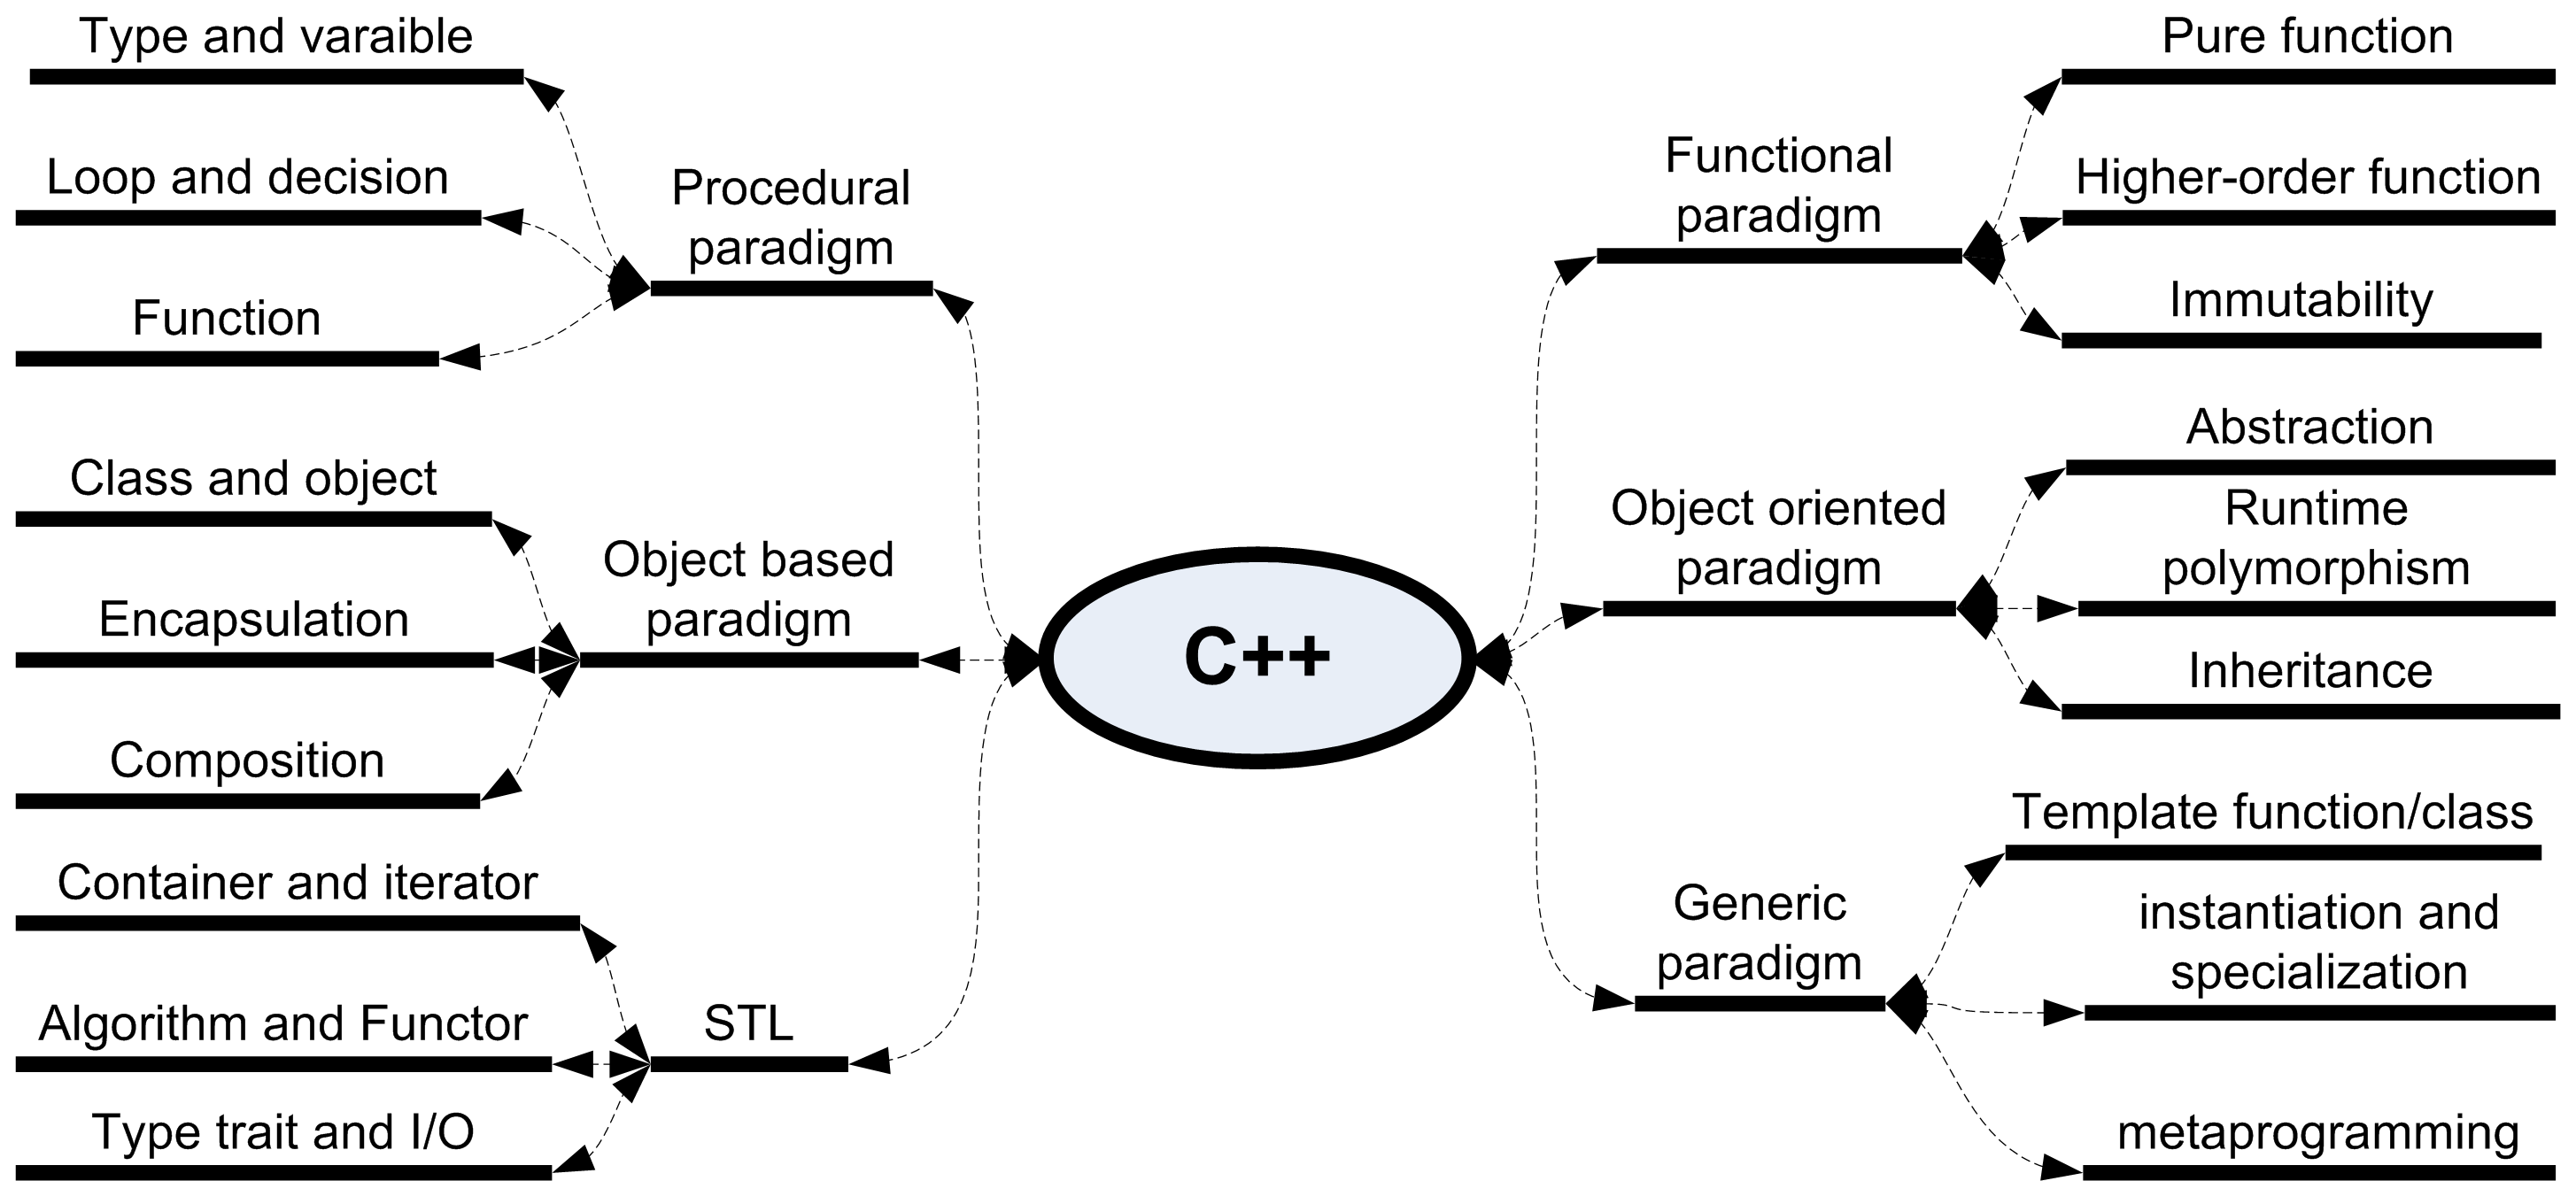
\includegraphics[width=0.95\linewidth]{pics/whole.png}
		\caption{The main components of C++ language}
		\label{fig:whole}
	\end{figure}

    \item There are three constraints in C++ language:1) compatible with C; 2) zero overhead abstraction; 3)static type. Some people also think the third constraint is value semantic. If you want to follow value semantic, you need to know the type information when you compile. So static type and value semantic are the two sides of one coin. These three constraints give C++ language very special characteristics. 
\end{itemize}

\subsection{Statement and expression}
\begin{itemize}
	\item Statement and expression are two important conceptions in C++ language, you can see their academic definition in cppreference.com. Although these two conceptions are theoretical, a lot of practical knowledge and conceptions, such as xvalue, reference etc., are defined on these two conceptions. That is why we need to understand them before we go deeper. An expression is a sequence of \textbf{operators} and their \textbf{operands}, which specifies a computation(calculation). The general operators are assignment, increment, arithmetic, logical, comparison and member access etc..
	
\begin{lstlisting}[numbers=none]
a=b, a+=b  //assignment
++a, a++  //increment
a+b, a&b  //arithmetic
a&&b, !a  //logical
a<b, a!=b  //comarision
a[b], a->b, a.b  //member access
\end{lstlisting}
	
	\item Statements are fragments of the C++ program that are executed in sequence. Statements which ends with semicolon are executed. C++ mainly includes the following types of statement: 1) expression statement, 2) compound statement, 3)selection statement(\texttt{if, switch}), 4)iteration statement(\texttt{while, for}) and 5)jump statement(\texttt{break,continue, return, goto}). Most statements are expression statements.
	
\begin{lstlisting}[numbers=none]
int n = 1;               // declaration statement
n = n + 1;               // expression statement
std::cout << n << '\n'; // expression statement
return 0;               // jump statement
\end{lstlisting}
	
\item Difference between statement and expression.
	\begin{enumerate}
		\item Expression: Something which evaluates to a value. Example: \texttt{1+2/x}
		
		\item Statement: A line of code which does something. Example: \texttt{GOTO 100;} and all statements are followed by a semicolon.
	
		\item The designers of C realized that no harm was done if you were allowed to evaluate an expression and throw away the result. In C, every syntactic expression can be a made into a statement just by tacking a semicolon along the end.
	
\begin{lstlisting}[]
x+y    //is expression;
x+y;   //is statement, but throw away the result
fun(i) //Function call is a expression, because it can yield a value.
b=c;   //This is statement. It has semicolon after it.
a=b=c  //b=c is an expression. 
\end{lstlisting} 
\begin{description}
	\item[Line 4:]  Statement represents an action-- assign a value to a variable.
	\item[Line 5:] \texttt{b=c} is expression, it yields value(\texttt{b}), then we can use this value for outside. In line 2, we assign value \texttt{b} to variable \texttt{a}. 
\end{description}
\end{enumerate}

\end{itemize}

\section{Compilation and link}

\subsection{Separate compilation and header file}
\begin{itemize}
	\item Having only one source file for a large project is unrealistic, so we break the code up into its logical structure. In this way, only changed parts need to be recompiled, and reduce the compile time. When we use the multiple source file, each part needs to know what information about functions and variables "used" from other files. That is why we need declaration, which lies in header file most of time.
	
	\item Even you can declare a variable, function and class many times, it's not good way to declare everywhere,\textbf{DO NOT copy declaration to the other positions in the other .cpp file. It leads to duplications and duplications are the bad smell in the code.} If you modify a declaration, you need to trace back all the declarations. If you need to use a function or variable in many different files, you should put them in a header filer. For example: \texttt{export\_to.h} for certain cpp source file or \texttt{global.h} file for the whole system. In a project, when you search function or variable declarations globally, if you find declaration statement more than two, It's strong indication to make a global head file and put these declaration statements into it.

	\item When you write a single source file (.cpp, .cxx, etc), your C++ compiler generates a translation unit. That is to say, \textbf{each .cpp will become a translation unit.} This is the object file from your source file plus all the header files which we use \texttt{\#include} statement in the source file.  A translation unit roughly consists of a source file after it has been processed by the \texttt{preprocessor}, meaning that header files listed in \texttt{\#include} directives are literally included, sections of code within \texttt{\#ifdef} may be included, and macros have been expanded.
	
	\item If you just want a function or variable visible to current translation unit. You can declare it as \texttt{static}. Or you can use unnamed namespace.  You don't need to put it into a header file.  Just remember in C++, you have to declare function and variable before you first use them. Different with C language, In C, compiler will guess a function prototype from it's usage, but it's not good coding style most of time in C++.
	
	\item A better suggestion is to have a single global.h file for a complex system. Then put some common type, defined type, constant and global function in this single global.h file. It will help to reduce duplication, just keep once appearance.
	
	\item Some good suggestions to write a header file:
	\begin{enumerate}
		\item "Everything" that should be exported (i.e., used in other files). "Nothing" that causes the compiler to immediately generate code.
		
		\item Use \texttt{\#pragma once} to add include guard, It's not standard, but it has been supported by many main stream compiler, such as: g++, clang and MSVC.

		\item const, template and inline function, which has \textbf{internal linkage.} In fact, you have to put template and inline function into a .h file. It's also good practice to \textbf{Put a semicolon in the end of head file.} Becuase you need semicolon after declare class. In .cpp file, no semicolon after each function definition.

		\item You should put the minimal set of \texttt{\#include} statements that are needed to make the header compilable. You can use forward declaration instead of including another header file. Or use more complicated PIMPL to achieve minimal set of others \texttt{\#include} in a header file. It decreases dependence.
		
		\item Basically, you should put each class definition into a single .cpp file, and make sure that each .cpp file has a corresponding .h file.  If two classes are highly correlated or very short, they maybe be put in the same .cpp file.

        \item \textbf{Don't} put "using directives" into the header files.
	\end{enumerate}

	\item Include header file in the following order. \textbf{Put your local/private header file in front of system header file. From specific to generic.} 
	\begin{enumerate}
		\item The prototype/interface header for this implementation (ie, the .h/.hh file that corresponds to this .cpp/.cc file).
		\item Other headers from the same project, as needed.
		\item Headers from other non-standard, non-system libraries (for example, Qt, Eigen, etc).
		\item Headers from other "almost-standard" libraries (for example, Boost)
		\item Standard C++ headers (for example, iostream, functional, etc.)
		\item Standard C headers (for example, cstdint, dirent.h, etc.)
	\end{enumerate}
	
    \item Why do we need to follow previous order?  This order makes some potential fault can be found as early as possible. Please see the below two examples, it demonstrate one idea:\textbf{explicit error is better than implicit success.}
	
	\begin{enumerate}

			\item When your local/private header is included on the first place, it makes your header file self-sufficient and self-sufficient avoids hidden dependency. We should include \texttt{Boo.h} the first place, because it makes compiling fail. If we include \texttt{Foo.h} first, although compile successively, it makes hidden dependency to \texttt{Foo} invisible, that is bad code smell. 

\begin{lstlisting}[numbers=none]
Foo foo;  //hidden dependency here //Boo.h
class Boo{
  ...
}

#include Foo.h //Boo.cpp
#include Boo.h 
\end{lstlisting}
			
			\item Sometimes, if you have your own function with same name as system or library, It can give you a compiler error; Below example will give you a compiler error. But if you put \texttt{<cmath>} before \texttt{myHead.h}. Then, main will use acos in cmath, and your acos will be override. The reason behind of this failure comes fomr \texttt{extern "c"}.
		
\begin{lstlisting}[numbers=none]
#include "myHead.h"  //double acos(double)
#include <cmath>
main{
	acos(0.5);
}

extern "C" double acos(double);
double acos(double); // compiler accept this order declaration.

double acos(double); 
extern "C" double acos(double); // compiler report error if see this order.
\end{lstlisting}
    		
	\end{enumerate}
	
	\item You can google "Advanced Software Engineering with C++ Templates". The first half part introduce separate compilation.
\end{itemize}

\subsection{Declaration and definition}
\begin{itemize}
	\item A declaration introduces an identifier and describes its type, be it a type, object, or function. \textbf{A declaration is what the compiler needs to accept references to that identifier.} 
	
\begin{lstlisting}
extern int bar;
extern int g(int, int); 
double f(int, double); //extern can be omitted for function declarations.
class Foo; //Foo foo is definition
\end{lstlisting}

\begin{description}
	\item[Line 1:] Add \texttt{extern} keyword before variable name. It makes the variable as declaration statement, not definition.
	
	\item[Line 4:] No \texttt{extern} is allowed for type declarations.
\end{description}
	
	\item A definition actually instantiates(implements) this identifier. It's what the linker needs in order to link references to those entities. These are definitions corresponding to the above declarations:

\begin{lstlisting}[numbers=none]
int bar;
int g(int lhs, int rhs) {return lhs*rhs;}
Foo foo {}; //put {}; after calss definition.
\end{lstlisting}
	
	\item The difference between declaring a symbol and defining a symbol:
	\begin{enumerate}
		\item A declaration tells the compiler about the existence of a certain symbol and makes it possible to \textbf{refer to that symbol everywhere where the explicit memory address or required storage of that symbol is not required.}  A definition tells the compiler what the body of a function contains or how much memory it must allocate for a variable.
		
		\item A symbol may be declared many times in different translation unit, but defined in on translation unit only once. For example, you can forward declare a function or class as many as  you want, but you may only ever have one definition for it. This is called the \textbf{One Definition Rule}.
	\end{enumerate}

\end{itemize}


\subsubsection{Forward declaration}
\begin{itemize}
	\item In C++, there exists the concept of forward declaring a symbol. We declare the type and name of a symbol so that we can use it where its definition is not required. There are three usages as below:
	\begin{enumerate}
		\item It will reduce compile-time dependencies --PIMPL.
		\item Hide all the implementation detail. 
		\item Break cyclic references
	\end{enumerate}
	
\begin{lstlisting}[numbers=none]
class C1; //That is a forward declaration.
class C2{
...
	C1* pc1;
}
\end{lstlisting}
	
	\item Forward declaration doesn't work if you need to build or access its member. It's only work when you refer it by pointer or reference. You need to write \texttt{\#include Foo.h}, so compiler can know the size and layout of \texttt{Foo} to compile below code.
\begin{lstlisting}[frame=single, language=c++]
class Foo; 
Foo* f1 = new Foo; //error,
	
fun(Foo* f1){
	f1->a;   //error, Compiler need to know if there is member a inside of Foo
}
fun(Foo f1)       //error, It's not a pointer or reference type.
\end{lstlisting}
	
	\item About cyclic include, you need to know below:
	\begin{enumerate}
		\item You can't write the code below, because it has cyclic dependent of \texttt{a.h} and \texttt{b.h}.
\begin{lstlisting}[numbers=none]
#include "b.h"
class A{
	B b;
}

#include "a.h"
class B{
	A a;
}
\end{lstlisting}

		\item In the end, you can use forward declaration to remove \texttt{\#include} statement. But at this time, you have to use pointer or reference in one class.
\begin{lstlisting}[numbers=none]
//a.h file, Don't need to include header file, because we use pointer later.  
class B; 
class A{
	B* b;
}
\end{lstlisting}
	\end{enumerate}
	
	\item About PIMPL(pointer to implementation), you need to know below:
	\begin{enumerate}
		\item Base on previous forward declaration, you can use "Pimpl" idiom.
\begin{lstlisting}[numbers=none]
class Widget { // "widget.h" file
private:
	struct Impl; // forward declaration here.
	Impl* pImpl;
};
		
#include "Foo.h"  // widget.cpp file, include Foo.h
struct Widget::Impl {
	Foo f1;
	...other detail.
};
\end{lstlisting}
		
		\item Pimpl Idiom is one of \texttt{std::unique\_ptr} most common use case. But just like using raw pointer,  you should define destructor even you have used \texttt{std::unique\_ptr}. 
		
\begin{lstlisting}
// widget.h file
class Widget { 
	Widget::~Widget()
	
private:
	struct Impl; // Forward declaration.
	std::unique_ptr<Impl> pImpl;
};
		
//widget.cpp file
#include "Foo.h" 
struct Wideget::Impl{
	Foo fo; 
}
Widget::~Widget() = default; 
\end{lstlisting}
\begin{description}
	\item[Line 3:] If you don't declare desctructor here, compiler will produce default destructor in line 8 by itself, In the end, it will call \texttt{delete struct* pIm} and \texttt{struct* pIm} is a uncompleted type(definition is still invisible here)
	
	\item[Line 15:] Here, \texttt{Widget}'s destructor can see the whole \texttt{Impl} definition(line 12), so \texttt{delete struct* pIm} is legal now. You don't need to define \texttt{Widget} destructor by youself, using default one is enough.
	
	\item[Source code:] The more explanation can be seen in "effective modern C++ item 22". 
\end{description}

\end{enumerate}
\end{itemize}

\subsection{Linkage}

\subsubsection{ODR}
\begin{itemize}
	\item For C language, there is tentative definition rule. You can define the same variable in two different .c file. The result will be undefined behavior. But in the C++, it is not legal any more(That is good). 
	
\begin{lstlisting}[numbers=none]
a.c
int g_i = 100;
//--------------------
b.c
int g_i;
fun(){
	printf("%d",g_i) //will print 100
}
\end{lstlisting}
	\begin{description}
		\item[gcc:] (gcc a.c b.c) report no error. in b.c, if you write \texttt{g\_i= 2}; gcc reports error.
		\item[g++:] (g++ a.c b.c) reports error.
	\end{description}

	\item In C++ language, tentative definition of variable is not allowed. At the same time, multi-definition of function is not allowed either. In the same unit, you can't define class C1 again, but if you put two class C1 in two different .cpp file. compiler doesn't complain at all. When you run the application, it probably crashes and it's dangerous. It's a little different with function and global variable, because function and global variable all need allocate memory.
	
	\item You need to follow this principle: \textbf{Either a name is for everyone (and declared in a header file) or is translation-unit-local in an anonymous namespace.} Detail can be found in "The One-Definition Rule  Andrzej's C++ blog".
\end{itemize}

\subsubsection{Duration, Scope and Linkage}
\begin{itemize}
	\item \textbf{Duration} and scope are two different conceptions in C++. there are three kinds of duration: \textbf{automatic, static and dynamic.}
        \item There are mainly three kinds of \textbf{scopes}:
	\begin{enumerate}
		\item global: In C++, we can use namespace to add more scopes to divide global scope.
		\item .cpp file: (translation unit).
		\item local: function local and class local. 
	\end{enumerate}

	\item Scope is a property handled by compiler, whereas linkage is a property handled by linker. There are two linkages: internal linkage and external linkage. Internal linkage refers to everything only in scope of a translation unit. External linkage refers to things that exist beyond a particular translation unit. In other words, accessible through the whole program, which is the combination of all translation units. Linkage refers only to elements that have addresses at link/load time; thus, class declarations and local variables have no linkage. \textbf{Only global scope variable or function definition has external or internal linkage. } Some internal and external linkage examples are:
	
\begin{enumerate}
	\item non-const global variable has external linkage. Use \texttt{static} to make it internal linkage. Please pay an attention here: \texttt{static} has two usages, in file scope, it says that a variable has \textbf{internal linkage}, in function or class scope, it says that this varaible has \textbf{static duration}.
	
	\item Const global variables have internal linkage by default.
	
	\item Functions have external linkage by default. \textbf{static function has internal linkage too}. Inline function will be introduced in the next section. 
\end{enumerate}

	\item \textbf{const variables internally link by default} unless otherwise declared as \texttt{extern}. It means that:
	\begin{description}
		\item[Many copies:] You can put \texttt{const int g\_num = 10;} into a header file or global.h file. Then when you need \texttt{g\_num,} just include this header file into you .cpp and it will not cause "multiple definition" linkage error. But most of time, const global variable are used in below context to avoid linkage error. 
\begin{lstlisting}[]
//a.cpp
const Buffer_Size = 10;
int a[Buffer_Size]

//b.cpp
const Buffer_Size = 20;
int b[Buffer_size]
\end{lstlisting}
		
		\item[One copy, global access:] You also can put \texttt{const int g\_num = 10;} in one .cpp file. then declare \texttt{extern const int g\_num ;} in global.h file.\textbf{Once you use extern to declare const, you change it to external linkage.} 
		
\begin{lstlisting}[numbers=none]
//file.h:
extern const int a_global_var;

//file.c:
#include "file.h"
const int a_global_var = /*const expression */;
\end{lstlisting}

		\item[One copy, local access:] If you really want to make const used just in one .cpp locally, use static and put it in the .cpp file.
	\end{description}
	
	\item When a definition has internal linkage, it means that:
\begin{enumerate}
		\item You can put two same static variable name in two different .cpp file, no linkage error. (Each definition will has his own memory, \textbf{Don't apply it on the large object.})
		
		\item You can't access internal linkage definition from another .cpp file. 
		
		\item You can't use \texttt{extern} with \texttt{static}, but you can use \texttt{extern} with \texttt{const}.
\end{enumerate}

\end{itemize}


\subsubsection{Inline function}
\begin{itemize}
	\item Usage of \texttt{inline} keyword is very simple: \textbf{No matter for member or non-member inline function, put it into a header file.} Why? 
\begin{enumerate}
	\item It’s imperative that the function’s definition (the part between the \{...\}) be placed in a header file, unless the function is used only in a single .cpp file. Because compiler need to see the definition, so it can expand and insert into soure code directly. In particular, if you put the inline function’s definition into a .cpp file and you call it from some other .cpp file, you’ll get an “unresolved external” error from the linker. 
	
	\item At the same time, no matter how you designate a function as inline, it is a request that the compiler is allowed to ignore: the compiler might inline-expand some, all, or none of the places where you call a function designated as inline. (Don’t get discouraged if that seems hopelessly vague. The flexibility of the above is actually a huge advantage: it lets the compiler treat large functions differently from small ones, plus it lets the compiler generate code that is easy to debug if you select the right compiler options.)
	
	\item Inline just suppress multi-definition error. It is programmer's responsibility to ensure that inline function definitions with the same name match exactly across translation units, to avoid all above bad result. You can see the best way is that putting an inline function into a header file.
\end{enumerate}
	
	\item In modern C++, inline tells the linker that, if multiple definitions (not declarations) are found in different translation units, they are all the same, and the linker can freely keep one and discard all the other ones. In another word, inline is mandatory if a function (no matter how complex or "linear") is defined in a header file, to allow multiple sources to include it without getting a "multiple definition" error by the linker.
	
	\item By default all the functions defined inside the class are implicitly or automatically considered as inline except virtual functions (Note that inline is a request to the compiler and its compilers choice to do inlining or not).
	
	\begin{enumerate}
		\item For non member function, put inline function into a header file, and when you need to use this function, include it.
		
		\item For member function, you have two options.
\begin{lstlisting}[numbers=none]
class Foo {  //option 1
public:
void method(){...};  //Give definition here
};

class Foo {  //option 2
public:
	void method(); //Don't put inline keyword here
};
inline void Foo::method(){  //Put inline keyword here
	...
}
\end{lstlisting}
	\end{enumerate}
	
	\item Does inline function has internal linkage? NO! The explanation is a little complex, so if you don't want go deeper, you can skip below contents. If you are confident and like facing challenge. In fact, \textbf{Inline function has external linkage,} but inline suppress multi-definition error, linker will just pick up anyone and discard others, that is dangerous. That is why we should make that we only have one definition, and that is why we should put inline function in header file. Once we want to use it, just include it. We demonstrate that inline has external linkage by below code. We have a.cpp and b.cpp two files.
\begin{lstlisting}
inline int foo() { //File a.cpp
	return 6;
}
void g() {
printf("foo called from g: return value = %d, address = %p\n", foo(), &foo);
}

inline int foo() { //File b.cpp
	return 12;
}
void g();
int main(){
	printf("foo called from main: return value = %d, address = %p\n", foo(), &foo);
	g();
}
\end{lstlisting} 
\begin{description}
	\item[Line 1 and 8 without inline:] it will trigger multi-definition linkage error
	\item[Line 1 and 8 one inline:] Only on inline, because inline has external linkage, so it will trigger multi-definition linkage error too.
	\item[Line 1 and 8 two inline:] Redefining an inline function with the same name but with a different function body is illegal; however, the compiler does not flag this as an error, but simply generates a function body for the version defined in the first file entered on the compilation command line, and discards the others. Therefore, may not produce the expected results.
	\item[Delete line 8 to 10:] Compiling error, identifier doesn't found.	
\end{description}

		
\end{itemize}


\subsection{Combine C and C++}
\begin{itemize}
	
	\item The key idea of this section is: \textbf{\texttt{extern "C"} disable name mangling.} C++ inherits basic data type, variable name, statement, expression, operator, control flow, function, file, head file and library, array, pointer and structure from C language. C++ is superset of C, so any C programs can be compiled by C++.
        
    \item When you use g++,  \texttt{\_\_cplusplus} will be defined automatically. (you can't undef it in fact.) When you use C compiler, such as gcc, \texttt{\_\_cplusplus} is not defined. At the same time, When you use C++ compiler, such as g++ to compile a C file, although file extension is .c, but g++ still use name mangling to change function name.  The conclusion is based on g++ and gcc on Linux system. \textbf{compiler will decide if \texttt{\_\_cplusplus} is defined, not based on source file name extension}
	
	\item The C++ compiler must be used to compile main(), and must be used to direct the linking process. \textbf{Most of time, you want your C++ application to call some existing C functions,} but not reverse. If you have c and cpp source files together, you can just use g++ compile them all. You don't need any \texttt{\_\_cplusplus} syntax.  g++ compiles all files using name mangling. (look them all as c++ files). At this time file extension doesn't play a role at all.
	
	\item If your C++ file want to use a c function. You don't have C function source code(It is in a lib or obj file) or you don't want to recompile it( it's a very big C library). At this time, you have three methods:
	

\begin{lstlisting}
extern "C"{  // method 1
	c_function(int);
}
	
extern "C"{  // method 2
	#include "old_C_header.h"
}
	
#ifdef __cplusplus  //method 3
extern "C" {
#endif
	Foo (int a, int b);
#ifdef __cplusplus
}
#endif
\end{lstlisting}
	\begin{description}
	\item[Line 9 to line 15:] If you can control the header file, you can use \texttt{\_\_cplusplus + extern "C"}. it will used both in C and C++ compiler. In fact, all c lib header file, such as \texttt{math.h} follow this pattern.
\end{description}

%	\item If you define a function in .cpp file(You have to use g++ to compile it), and this function will be used in legacy C system, you need to use \texttt{\_\_cplusplus + extern "C".} to disable name mangling.  You can give lib and head file to C system,  and then the C system can include head file and linked to lib.
	
%	\item \textbf{In one word, if you have obj code produced by C or C++, When you want to linked it to different language, you should consider using \_\_cplusplus + extern "C" }
	
	\item Can a C function directly access data in an object(lib or so) of a C++ Class. Yes,but with some restriction. C++ class has no virtual base and virtual function. no access control. If you just want to pass a object from or to C function, you can refer a article in "C++ FAQ, 36.05". It demonstrate how to pass object from main to cppCallingC (C++ to C), then call cCallingC++(C to C++). Pay attention to two points:
	\begin{enumerate}
		\item We pass the class pointer.
		\item we use the same header file, but use \texttt{\#ifdef \_\_cplusplus} to defines one class(used by C++) and one struct(used by C), and they have the same name.
	\end{enumerate}
	
	\item There are two occasions which you need to use \texttt{extern "C"}:
	\begin{enumerate}
		\item When you want to produce a DLL or SO. Why, because maybe your DLL or SO will be used in both C language and C++ language. Or different compiler which uses different name mangling rule.
		
		\item When the code will be used by java, python or legacy C code.
	\end{enumerate}
\end{itemize}


\chapter{type, operator and expression}
\section{type}
\subsection{Type cast in c++}
\subsubsection{Implicit conversions}
\begin{itemize}
\item There are two kinds of conversion, one is \textbf{implicit}, and the other is \textbf{explicit}. Implicit conversions are performed whenever an expression of some type \texttt{T1} is used in context that does not accept that type, but accepts some other type \texttt{T2}; in particular:
	\begin{enumerate}
		\item when the expression is used as the argument when calling a function that is declared with \texttt{T2} as parameter;
		\item when the expression is used as an operand with an operator that expects \texttt{T2};
		\item when initializing a new object of type \texttt{T2}, including return statement in a function returning \texttt{T2};
		\item when the expression is used in a switch statement (\texttt{T2} is integral type);
		\item when the expression is used in an if statement or a loop (\texttt{T2} is bool).
	\end{enumerate}
	
	\item Implicit conversion sequence consists of the following, in this order:
	\begin{enumerate}
		\item zero or one standard conversion sequence;
		\item zero or one user-defined conversion;
		\item zero or one standard conversion sequence.
	\end{enumerate}

	\item user-defined conversion is an user-defined conversion consists of zero or one non-explicit single-argument converting constructor or non-explicit \textbf{conversion operator} call. You can think that conversion operator is the opposite of a one-argument conversion constructor.
\begin{lstlisting}[numbers=none]	
struct X {
	//implicit conversion
	operator int() const { return 7; }
	
	// explicit conversion
	explicit operator int*() const { return nullptr; }
	int* p = static_cast<int*>(x); // OK: sets p to null
	//  int* q = x; // Error: no implicit conversion
	
	//   Error: array operator not allowed in conversion-type-id
	//   operator int(*)[3]() const { return nullptr; }
	using arr_t = int[3];
	operator arr_t*() const { return nullptr; } // OK if done through using
	//  operator arr_t () const; // Error: conversion to array not allowed in any case
};
\end{lstlisting}	
	
	\item An example and explanation. In line 9, \texttt{ref(a)} return a \texttt{reference\_wrapper} type object. so in line 3, \texttt{++a} is \texttt{++reference\_wrapper}. Right now \texttt{a} (type is \texttt{reference\_wrapper}) is used in context "used as an operand with an operator that expects \texttt{T2}", so compiler can perform implicit conversion. Then it looks for "zero or one non-explicit single-argument converting constructor or non-explicit conversion function call", In the \texttt{reference\_wrapper}, we define \texttt{operator T\& () const}, so it changes it to \texttt{int\&} which supports ++. That is the whole process. 
\begin{lstlisting}[]
template<typename T>
void functest(T a){
	++a;
}

int a = 1;
functest(a);  //a is still 1
functest(ref(a)); // a is 2 now.	 
\end{lstlisting}	
	
	\item Class implicit conversion can happen when it has:
	\begin{enumerate}
		\item Single constructor, it means that a class can be produced \textbf{from something.}
		\item Operator Type, it means that a class can be converted \textbf{to something.} convert class to basic type, you need \texttt{operator basicTypeName}, no argument, and must be member function.

\begin{lstlisting}
class A {
	A(int i); // bad style
	operator const char*(); //bad style
};
	
A a1, a2;
a2 = a1*2;   // implicitly convert 2 to temp A obj.
a2 = 2;   //implicitly convert 2 to temp A obj, then call operator =;
\end{lstlisting}
	\end{enumerate}
	
	\item Implicit conversion can be called by compiler implicitly, (means that you don't know at all). It sometimes will lead to potential ambiguity problem and result which you don't expect. more detail can be seen effective c++ item 26.
\begin{lstlisting}[frame=single, language=c++]
class A{
	A(class B&);
};
class B{
	operator A()
};
	
void g(const A&);
B b;
g(b)
\end{lstlisting}
\begin{description}
	\item[Line 10:]	It can call A's constructor in class A, or it can call B's operator A() in class B. Compiler stops because of ambiguity.
\end{description}	
	
	\item \textbf{You should always avoid implicit conversion, and there are two rules you need to follow.}
	\begin{enumerate}
		\item use explicit before single parameter constructor. In the code below, with explicit keyword before constructor,  you have to use \texttt{A(2)} or \texttt{(A)2} to explicitly build a A temporary obj in \texttt{a1*A(2)} expression. It's a good habit and you should follow. 
		
		\item use name convert function instead of  "operator Type". So string class in STL has a function \texttt{c\_str()} instead operator \texttt{char*()} const. 
	\end{enumerate}
\begin{lstlisting}[numbers=none]
class A {
	explicit A(int i);     // good
	const char* getInternalPoint(); //good,a name function.
};	

A a1;
a2 = a1*A(2) // a2 = a1*2 will fail. 
\end{lstlisting}	
	
\end{itemize}

\subsubsection{Type cast operator}
\begin{itemize}
	\item Unrestricted explicit type-casting allows to convert any pointer into any other pointer type, independently of the types they point to.  (syntax and compiling is right, but cause run-time error). In order to overcome this problem,  in C++ langauge, we introduce c++ cast operator, There are five cast operators, \texttt{dynamic\_cast}, \texttt{const\_cast} and \texttt{static\_cast}.\textbf{You should always use them in C++.}. \texttt{reinterpret\_cast} and \texttt{bit\_cast} are not used very often. It mainly used in some specific context.
\begin{lstlisting}[frame=single, language=c++]
char c = 10;    
int *p = (int*)&c;  //compile succeed here
*p = 5;             //but run time error later and cause stack corruption.
	
int *p = static_cast<int*>(&c); //compile fail here, more safe. 
\end{lstlisting}
		
	\item \texttt{void*} type can be converted to any other type implicitly. You don't need any cast operator when you change any type pointer to \texttt{void*}, But when you want to use dereference \texttt{void} pointer , you'd better use \texttt{static\_cast }to change it back to a certain type pointer.
\begin{lstlisting}[frame=single, language=c++]
int* p = malloc(sizeof(int));
int* p = static_cast<int*>(malloc(sizeof(int)));
\end{lstlisting}		
		\begin{description}
			\item[Line 1:] \texttt{malloc} return void*, so you can assign it to \texttt{int *} directly in C language.
			\item[Line 2:] In C++, you have to use cast operator. A better way is to use \texttt{new} instead.
		\end{description}

	\item Using \texttt{const\_cast} is not good design. Sometimes for a const member function, you have to use \texttt{const\_cast} to change this pointer to modify a class member. If compiler support, always use \texttt{mutable}  keyword.  Only use \texttt{const\_cast} if your compiler doesn't support \texttt{mutable}. Sometimes, For some legacy functions, You have a const object you want to pass to a function taking a non-const parameter, and you know the parameter won't be modified inside the function. The second condition is important, because it is always safe to cast away the constness of an object that will only read, not modify. At this time, you can use \texttt{const\_cast}.

\begin{lstlisting}[numbers = none]
strlen( char* p);
const char* cp = "hello";

strlen(const_cast<char*>(cp));	
\end{lstlisting}

	\item Changing the value of an const object through \texttt{const\_cast} pointers leads to  "undefined behavior". For const static data -- the compiler may put such variables in a read-only region, the program will crash if you try to modify it.

\begin{lstlisting}[numbers = none]
const int a = 12;
int* p = const_cast<int*>(&a); //Bad style
*p = 66;  //UB
\end{lstlisting}

	\item \texttt{static\_cast<type-name>} expression will be valid only if type-name can be converted implicitly to the same type that expression has.  It will stop you from change a bird class to an apple class which is a totally unrelated class.  Even changing int to double, encourage you to use \texttt{static\_cast<double>(i)}.  It can help you to find cast easily in you source code by search \texttt{static\_cast}.
\begin{lstlisting}[numbers = none]
int i = 11111600;
char c = i; //give warning
char c = (char)i; //no warning, because you have told compiler.
char c = static_cast<char>(i); //no warning, just like previous statement

int *p = (int* p)i //no warning, but crash when running
int *p = static_cast<int *>i //compile error, 
//That is why static_cast is better then C style const.
\end{lstlisting}

%	\item  \texttt{static\_cast} can't deal with inheritance well in C++. 
%\begin{lstlisting}[numbers = none]
%struct V {
%	virtual void f() {};
%};
%struct A : V {};
%struct B : V {};
%
%A a;
%V& v = a;
%B& b = static_cast<B&>(v); //compile OK, but it's UB.
%\end{lstlisting}
%\begin{description}
%	\item[Source code] From \texttt{V} to \texttt{B}, it's possible to downcast, so \texttt{static\_cast} succeed. But if \texttt{A} is behind reference \texttt{V}, then you will have undefined behaviour. That is why we need \texttt{dynamic\_cast}.
%\end{description}	
	
	\item A child pointer can always be assigned to base pointer directly, that is the \textbf{up-cast} conversion and how polymorphic implements. \texttt{dynamic\_cast} use to \textbf{down-cast} a base pointer to child pointer. \texttt{dynamic\_cast} assure that down cast is valid. \texttt{dynamic\_cast} can also used in reference type. When cast fail, it will not return nullptr, (because it's reference), just throw a \texttt{bad\_cast} exception.
	
\begin{lstlisting}
struct A {};
struct D : public A {};

D d; // the most derived object
A& a = d;
D& new_d = dynamic_cast<D&>(a); // downcast	
\end{lstlisting}	
	\begin{description}
		\item[Line 5:] That is up-cast,\texttt{ dynamic\_cast} may be used, but unnecessary.
		\item[Line 6:] That is down-cast, you have to use \texttt{ dynamic\_cast} to make sure it can be down-cast properly.
	\end{description}
	
	\item \texttt{dynamic\_cast} should only be used down-cast public inherited relationship. You can't use \texttt{dynamic\_cast} when it is not private or protected inherited relationship. If a class doesn't have virtual function, you can't use \texttt{dynamic\_cast} on this object either.

	
	
	\item If you frequently use \texttt{dynamic\_cast}, It can be a sign that your base class offer too little functionality, you'd better to re-design you base class API(adding more member function to base class.)
	
	\item \texttt{dynamic\_cast} can also be used in \textbf{side-cast in multi inheritance. }
\begin{lstlisting}[frame=single, language=c++, mathescape=true]
struct V {
	virtual void f() {}; // must have virtual function
};
struct A : virtual V {};
struct B : virtual V {};
struct D : A, B {};
	
D d; // the most derived object
A& a = d; // upcast 
B& b = dynamic_cast<B&>(a); //sidecast
	\end{lstlisting}
\begin{description}
	
	\item[Line 9:] That is side cast. Change \texttt{d} to \texttt{a} first(from child D to parent A), then \texttt{a} to \texttt{b}, (from child D to parent B, always succeed becasue \texttt{d} is behind \texttt{a}, and \texttt{d} can be changed to \texttt{b} )
	
\end{description}
	
	\item \texttt{dynamic\_cast} different with \texttt{static\_cast}: 1) \texttt{static\_cast} check on compile time. 2) \texttt{static\_cast} no run time information, so sometimes it makes mistake.
\begin{lstlisting}[frame=single, language=c++, mathescape=true]
class A {
	public:
	int i;
	virtual void fun(){cout<<"base"<<endl;}
};

class B : public A {
	public:
	virtual void fun(){cout<<"child"<<endl;}
};

A* pa = new B();
pa->fun();
B* pb = dynamic_cast<B*>(pa); //OK, because B is behind base pointer pa,
B* pb = static_cast<B*>(pa);  //OK, 	

A* pa = new A();
pa->fun();
B* pb = dynamic_cast<B*>(pa); //return nullptr, A is behind base pointer pa, 
B* pb = static_cast<B*>(pa);  //UB, that is not good.on my VS, it print "base"
\end{lstlisting}
\begin{description}
	\item[Line 17 to 20]  when A is behind base pointer, When you downcast to B, dynamic give you nullptr(warning), but static run into UB.	
\end{description}

	\item \texttt{static\_cast} can not be use in virtual base 
\begin{lstlisting}[numbers = none]
struct Parent {
virtual void f() {};
};
struct Child : virtual Parent {};

Child child;
Parent& parent = child;
Child& other = static_cast<Child&>(parent); //compile fail, 
\end{lstlisting}

	\item About \texttt{dynamic\_cast}, "exceptional C++" item 44 give a good question and answer.
	
	\item \texttt{reinterpret\_cast} can converts any pointer type to any other pointer type, even an totally unrelated classes. The operation result is a simple binary copy of the value from one pointer to the other. All pointer conversions are allowed: neither the content pointed nor the pointer type itself is checked. It can also cast pointers to or from integer types. \textbf{DON'T USE IT UNLESS YOU ARE IN THE CORNER.} When you use \texttt{reinterpret\_cast} change one type pointer to another type pointer, it violate "strict alias rule" and will lead to UB(undefined behavior).
	
	\item First off, yes, this results in undefined behavior because there is no \texttt{SomePod} object within the buffer. Objects do not spontaneously come into existence just because you want them too; The compiler determines that the store to the x subobject cannot possibly alias the object buffer, because buffer does not contain an x subobject, and no other object for which buffer might provide storage has been created since buffer was created. Therefore the compiler reasons that it can reorder the store to before its internal marker for the start of the lifetime of buffer. The store can now be deleted, because it is immediately followed by the start of the lifetime of an object in the same region of storage.
\begin{lstlisting}
struct SomePod { int x; };
alignas(SomePod) char buffer[sizeof(SomePod)];
reinterpret_cast<SomePod*>(buffer)->x = 42;
\end{lstlisting}

	\item In order to avoid previous UB of \texttt{reinterpret\_cast}, we can use memcpy to make sure that there is no UB problem. 
\begin{lstlisting}
struct SomePod { int x; };
alignas(SomePod) char buffer[sizeof(SomePod)];
SomePod temp;
memcpy(&temp, buffer, sizeof(SomePod));
temp.x = 42
memcpy(buffer, &temp, sizeof(SomePod));	
\end{lstlisting}

	
	\item If you understand previous \texttt{reinterpret\_cast} and memcpy, you can understand \texttt{std::bit\_cast} intent. \texttt{std::bit\_cast} also use memcpy inside, it also can be used in constexpr context.  it is a new feature of C++ 20.
	
	\item Conclusion:
\begin{enumerate}
	\item \texttt{const\_cast} should be used when you call legacy or old function without const parameter. 
		
	\item Four kinds of casts: 1)implicit cast, 2)C typle cast, 3)\texttt{static\_cast} and 4)\texttt{dynamic\_cas} they becomes more restricted and more safe. 
	
	\item \texttt{static\_cast} will suppress warning, and not allow (\texttt{int} ->\texttt{int *}) conversion. That is why we should always use \texttt{static\_cast}. 
	
	\item \texttt{static\_cast} ALWAYS allow downcast,(because it's OK theoretically). That is why we need to use \texttt{dynamic\_cast}. \texttt{dynamic\_cast} only can be used with inheritance class with virtual function. 
\end{enumerate}

	
\end{itemize}

\subsection{RTTI}
\begin{itemize}
	\item It's a relatively new conception in C++, you should avoid using it on old C++ compiler. It has two methods: \texttt{typeid} and \texttt{dynamic\_cast}. There are two kinds of types (for the purposes of RTTI): polymorphic types and non-polymorphic types. A polymorphic type is a type that has a virtual function, in itself or inherited from a base class. A non-polymorphic type is everything else; this includes POD types and many other types too.
	
	\item \texttt{typeid} operator will return a \texttt{type\_info} class.  You need to include typeinfo.h head file. \texttt{typeid} operator also receive pointer or class name. \texttt{name} is member function of \texttt{type\_info}.
	
\begin{lstlisting}
int myint = 50;
std::string mystr = "string";
double *mydoubleptr = nullptr;
	
cout << "myint has type: " << typeid(myint).name(); //typeid is operator
cout<< "mystr has type: " << typeid(mystr).name();  // it returns type_info
cout<< "mydoubleptr has type: " << typeid(mydoubleptr).name(); 
\end{lstlisting}
 	
	\item RTTI has legitimate uses but is prone to abuse, so you must be careful when you use it. Just like exception, It has some loss in performance, you can use flag "-fno-rtti" to turn off it. You may use RTTI freely in unittests, but avoid it when possible in other code. consider one of the following alternatives to querying the type:
	\begin{enumerate}
		\item Virtual methods are the preferred way of executing different code paths depending on a specific subclass type. This puts the work within the object itself.
		
		\item If the work belongs outside the object and instead in some processing code, consider a double-dispatch solution, such as the Visitor design pattern. This allows a facility outside the object itself to determine the type of class using the built-in type system. Visitor design pattern can be seen in the later section.
	\end{enumerate}
\end{itemize}


\subsection{Arithmetic types}
\subsubsection{Numerical Overflow}

\begin{itemize}
	\item How to understand integer overflow problems? \texttt{x} is a position in the below figure, \texttt{x+3} means walk 3 step clockwise from \texttt{x.} \texttt{x-3} means walk 3 step anti-clockwise from \texttt{x}. The overflow only happen in the -8 position. Anytime you walk pass the -8 position, the overflow happens, no matter clockwise and anti-clockwise direction. For example, 5+4 = -7(not 9); -6-3 = 7(not -9).

	
	\begin{center}
		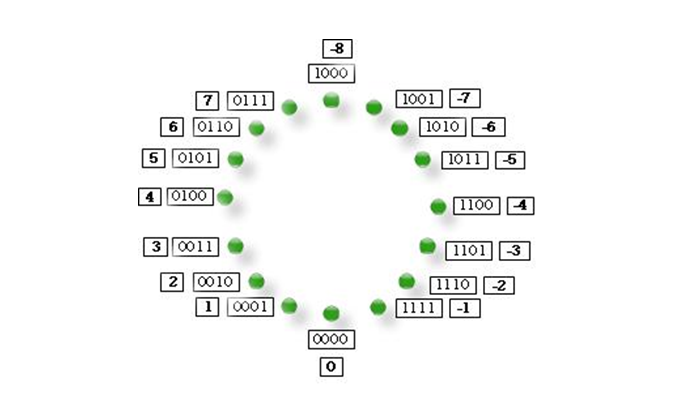
\includegraphics[width=0.5\linewidth]{pics/integer.png}
		
		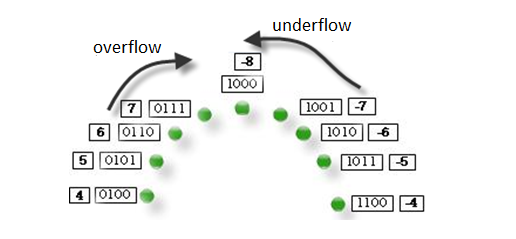
\includegraphics[width=0.5\linewidth]{pics/integer1.png}
	\end{center}
	
	\item Integer type has \textbf{overflow} problem, and float has \textbf{precision} problem. So prefer to use \texttt{long long} and \texttt{double} as your numerical type. In modern hardware, memory usage is not big concern, type with enough width can save you a lot of trouble in the future. 
	
	\item In C and C++, you can use limits.h or <limit> to get all the type limit information.
	
\begin{lstlisting}[numbers=none]
INT_MAX //use in C
INT_MIN

std::numeric_limits<int>::lowest() //use in C++
std::numeric_limits<int>::max()
\end{lstlisting}
	
	\item There are three ways to deal with overflow:
	\begin{enumerate}
		\item Build your own template function.
\begin{lstlisting}[numbers=none]
template <class T>
void increment_without_wraparound(T& value) {
	if (value < numeric_limits<T>::max())
	value++;
}
\end{lstlisting}
		
		\item  Judge if overflow happens before calculation.
		
\begin{lstlisting}
if ((x > 0) && (a > INT_MAX - x)) // a + x would overflow 
if ((x < 0) && (a < INT_MIN - x)) // a + x would underflow

if ((x < 0) && (a > INT_MAX + x)) //a - x would overflow  (1-(-10))
if ((x > 0) && (a < INT_MIN + x)) //a - x would underflow (1-10)

if (a > INT_MAX / x)  // a * x would overflow 
if ((a < INT_MIN / x)) // a * x would underflow 
\end{lstlisting}
		\begin{description}
			\item[Line 1:] a is point, \texttt{x>0} means that \texttt{a+x} is clockwise turning, then it will overflow
			\item[Line 2:] a is point, \texttt{x<0} means that \texttt{a+x} is anti-clockwise turning,  so it will underflow It's easy to understand according to previous figure.
		\end{description}
		
		\item Judge it after calculation.
\begin{lstlisting}[numbers = none]
uint32 a,b;
uint32 result = a + b;
if (result < a) //overflow
\end{lstlisting}
	\end{enumerate}
	
	\item There's no simple, general, portable way to avoid integer overflow. You can't safely check whether a signed integer addition or subtraction overflowed after the fact. An overflow in signed arithmetic causes undefined behavior. Typically the result wraps around, but in principle your program could crash before you have a chance to examine the result. Clang 3.4+ and GCC 5+ offer checked arithmetic builtins. They offer a very fast solution to this problem, especially when compared to bit-testing safety checks.
\begin{lstlisting}[frame=single, language=c++]
unsigned long b, c, c_test;
if (__builtin_umull_overflow(b, c, &c_test)){
	// returned non-zero: there has been an overflow
}
\end{lstlisting}
	
	\item When you do some calculation, you can have some tricks to avoid overflow. If you  want to know the last three digits of \texttt{n!}. You need use \texttt{mod} to keep last two digits in each calculation.
\begin{lstlisting}[numbers = none]
(a+b)/2  //a+b maybe overflow
a/2+b/2 +(a&b&1);
\end{lstlisting}
	
\end{itemize}

\subsubsection{Numerical conversions}
\begin{itemize}
	\item Numerical conversions happen in three contexts:
	\begin{enumerate}
		\item Assign a value of one \textbf{arithmetic type} to a variable of another arithmetic type.
		
		\item Combine mixed types in expressions.(Most of time, implicit conversion)
		
		\item Pass arguments to or return from a function with different type.
	\end{enumerate}
	
	\item convert short type to long type is \textbf{promotion}, it happens when we need hardware bit alignment optimization. Most of time, we don't need to worry about it. In an expression, C++ makes three kinds of automatic promotion conversion.
	\begin{enumerate}
		\item Some types are automatically converted whenever they occur. For example, when you add \texttt{char} to \texttt{char}. C++ converts \texttt{bool}, \texttt{char}, \texttt{unsigned char}, \texttt{signed char} and \texttt{short} to \texttt{int}. Because \texttt{int} type is generally chosen to be the computer's most natural type. \textbf{It does calculations faster for that type.} It's called \textbf{integer promotions.}
		
		\item Some type are converted when they are combined with other types in an expression. When an operation involves two types, the smaller is converted to the larger. For example, when you add an \texttt{int} to a \texttt{float}, \texttt{int} is converted to \texttt{float} type. (You have to do it, because two types have the different inside binary representations.)
		
		\item \texttt{unsigned short} convert to \texttt{int} if \texttt{short} is shorter than \texttt{int}, if they have the same size. \texttt{unsigned short} convert to \texttt{unsigned int}.  So no data loss in promoting.
	\end{enumerate}
	
\begin{lstlisting}
char c1, c2, c //c1 and c2 convert to int first.
c = c1+c2;  // then change int result back to char.

/*  LLVM IR code below
store i8 97, i8* %c1, align 1
store i8 2, i8* %c2, align 1
%0 = load i8, i8* %c1, align 1
%conv = sext i8 %0 to i32
%1 = load i8, i8* %c2, align 1
%conv1 = sext i8 %1 to i32
%add = add nsw i32 %conv, %conv1
%conv2 = trunc i32 %add to i8 */

i+f // i will promoted to f

float f1, f2, f
f = f1+f2 
\end{lstlisting}
	
	\begin{description}
		\item[Last line:] whether \texttt{f1} change to double depends on compiler. clang++ has fadd in LLVM IR, so it doesn't change \texttt{f} to double.
	\end{description}
	
	\item A implicit conversion will happen when you assign value to a bool, zero converts to false, and nonzero converts to true.
	
	\item When a implicit conversion happen, assigning a value to a type with a greater range usually poses no problem. If shorter range or different type, maybe there are some problems. For example, when conversion \texttt{double -> float, long long ->float} happens, it maybe lose precision. When \texttt{float -> i} happens, it loses fragment. It even bring undefined behavior when you have below code: \texttt{int i = 666; char c = i;}.
	
\begin{lstlisting}
int i, float f = 3.99;
i=f;  //i will be 3(not rounding), UB if f is too big

f = i; //will lost precision if i is big.
\end{lstlisting}
	
	\item A implicit conversion also happen when you call a function.(Just like you use assignment operator=). Below they all compile successfully. Compile with -Wconversion flag, it doesn't included in -Wall in g++; It just give warning when standard conversion happen. (no warning for promotion conversion).

\begin{lstlisting}[numbers=none]
bool isLucky(int number);

isLucky('a') // promotion ,NO warning
isLucky(false) // promotion, NO warning
isLucky(1.2f) //standard conversion.  Warning
\end{lstlisting}
	
	\item In C++, introduce braces initialization \{\}, It will not allow narrowing happen. But in g++, it just show a -Wnarrowing message, Anyway, I think that it's helpful.
\begin{lstlisting}[numbers=none]
int x = 66;  char c1 = {x}; //ok	
int x = 666; char c2 = {x};// not allowed;

int fun(){
	return 1.2f; //OK, no warning
	return {1.2f}; //ERROR, -Wnarrowing
}
\end{lstlisting}
	
	\item In order to suppress conversion warning, you can use explicit numerical conversion to state your intention clearly and loudly. In C language, there exist two main syntax for explicit type-casting: functional and C-style cast.  \textbf{Prefer C-style cast in C language}. In C++ language, \textbf{You should always use \texttt{static\_cast}}.
	
\begin{lstlisting}[]
double x = 10.3;
int y;
unsigned int n1 = (unsigned int)f; // C-style cast
unsigned int n2 = unsigned(f);     // functional cast
int b = static_cast<int>(f);  //explicit C++ style
\end{lstlisting}
	\begin{description}
		\item[Line 4:] functional cast only be used in one word type. \texttt{unsigned int (f)} is not right, \texttt{int *(p)} is not right either. That is why we prefer C-style cast in C language.
	\end{description}
\end{itemize}

\subsection{size\_t and ptrdiff\_t}

\subsubsection{Be careful with unsigned int}
\begin{itemize}

    \item When an \texttt{unsigned int} and an \texttt{int} are added together, the \texttt{int} is first converted to \texttt{unsigned int} before the addition takes place and the result is also an \texttt{unsigned int}. In another word, For integer addition or subtraction, It is just a trip around clock. When you reach a position in the clock, how to understanding depends on its context and type.
\begin{lstlisting}[numbers=none]
unsigned int ui = 0xfffffffe  // -2 or UNIT_MAX-1
int i = 1;
//ui+i will be expreseed 0xffffffff in memeory. 
printf("%d", ui+i); //print -1
printf("%u", ui+i); //print UINT_MAX;	
cout<<ui+i<<endl; //output 4294967260
(ui+i)<6  //false here, interpret it as unsigned int
\end{lstlisting}
    
	\item You can see llvm reference. \textbf{1) only i32, no ui32 2) only add}.  3) but has umultiply and uge and zext or sext. That is to say, these three operations need interpret signed semantic differently.  About umultiply and zext, please visit: \verb|https://llvm.org/docs/LangRef.html| to get more detail.
	 
\begin{lstlisting}[frame=single, language=c++]
unsigned int ui = -2 // or UNIT_MAX-1
int i = 1;
(ui+i)/4  //a big positive number
int* p;
p+(ui+i);  //on 32 bits, this ok, 
\end{lstlisting}

\begin{description}
	\item[Line 5:] On 64 bits, \texttt{ui+i} will be promote to 64 bits first. At this time, it will be promoted according to \texttt{unsigned int}. For \texttt{p+(ui+i)} questions, we can use \texttt{size\_t} and \texttt{ptrdiff\_t} type. 
\end{description}
	
    \item In summary, \texttt{ui+i} result type is \texttt{unsigned int},  when you use \texttt{ui+i} in 1) compare with other, 2) promote 3) multiply or sub, it will interpret according to its unsigned semantic(non negative). Maybe it's not what you expect.  In one word, \textbf{Don't use unsigned type just for big range, if int is not big, just use long, don't use unsigned int. Don't combine unsigned and signed type together.}	
\end{itemize}

\subsubsection{size\_t}
\begin{itemize}
	\item The main reason of \texttt{size\_t} is: size of something is dependent on pointer, but on different system, size of pointer is not same as size of int.  \textbf{But size of pointer is always same as size\_t}. The size of \texttt{size\_t} and \texttt{ptrdiff\_t} always coincide with the pointer's size. Because of this, it is these types which should be used as indexes for large arrays, for storage of pointers, pointer arithmetic, loop counters, array indexing, and address arithmetic.

	\item Why we need \texttt{size\_t?}, Semanticlly, it should be pointer type, but physically, it's a kind of integer, so when we use \texttt{int} or \texttt{short} or \texttt{long} to represent, it will cause cross-plat-form problem. \textbf{In one word, int is not always same as bits of OS. but size\_t and ptrdiff\_t are always same.}

	\item Type \texttt{size\_t} is a typedef that's an alias for some unsigned integer type, typically \texttt{unsigned int} or \texttt{unsigned long}, but possibly even \texttt{unsigned long long}. Each Standard C implementation is supposed to choose the unsigned integer that's big enough--but no bigger than needed--to represent the size of the largest possible object on the target platform.
	
	\item Using \texttt{size\_t} appropriately makes your source code a little more self-documenting. When you see an object declared as a \texttt{size\_t}, you immediately know that it represents a \textbf{size} in bytes or an \textbf{index}, rather than an error code or a general arithmetic value.
	
	\item \texttt{ptrdiff\_t} type is a base signed integer type of C/C++ language. The type's size is chosen so that it can store the maximum size of a theoretically possible array of any type. On a 32-bit system \texttt{ptrdiff\_t} will take 32 bits, on a 64-bit one 64 bits.
\begin{lstlisting}[numbers=none]
int A = -2;   // should use ptrdiff_t here
unsigned B = 1; // should use ptrdiff_t here.
int array[5] = { 1, 2, 3, 4, 5 };
int *ptr = array + 3;
ptr = ptr + (A + B); //Error on 64 bit OS
printf("%i\n", *ptr);
\end{lstlisting}
	
	\item A good article is "Why size\_t matters", another one is "About \texttt{size\_t} and \texttt{ptrdiff\_t".} just google and read them!   
\end{itemize}

\subsection{Aggregate and POD type}
\subsubsection{Aggregate}
\begin{itemize}
	
	\item \textbf{The basic idea of Aggregate type is that you can use aggregate list initialization}. All the detail definition of an aggregate can be traced back to this main purpose. In source code level, an aggregate is an array or a class with no user-declared constructors, no private or protected non-static data members, no base classes, and no virtual functions.
\begin{lstlisting}[numbers=none]
class NotAggregate1{
	int x; //x is private by default and non-static
	virtual void f() {} //remember? no virtual functions
};
		
class Aggregate1{
private:
	void f() {} // ok, just a private function
};
\end{lstlisting}

	\item In C++11, Previously, an aggregate could have no user-declared constructors, but now it can't have user-provided constructors. Is there a difference? Yes, there is, because now you can declare constructors and default them:
\begin{lstlisting}[numbers=none]
struct Aggregate {
	Aggregate() = default; 
};
\end{lstlisting}

	\item In C++11, Now an aggregate cannot have any brace-or-equal-initializers for non-static data members. What does this mean? Well, this is just because with this new standard, we can initialize members directly in the class like this:
\begin{lstlisting}[numbers=none]
struct NotAggregate {
	int x = 5; // valid in C++11
	std::vector<int> s{1,2,3}; // also valid
};
\end{lstlisting}

	\item  An aggregate class can have a non-aggregate data member. Because it will not stop us from using aggregate initialization for the aggregate class. You can see the example code below, value in brace list can be used to call non-aggregate user define constructor. So for class \texttt{Test}, it is still aggregate type.
\begin{lstlisting}[]
class Foo{
public:
    Foo(int i): i_{i}{ };
    int i_;
};

struct Test{
    Foo f;
    int k;
};

cout<<is_aggregate_v<Foo><<endl; //No, because we have user define constructor
cout<<is_aggregate_v<Test><<endl; //Yes, it can include non-aggregate.
Test t = {1,2}; //can use aggregate init here.
\end{lstlisting}

	\item Now let's see how aggregates are special. They, unlike non-aggregate classes, can be initialized with curly braces \{\}. 
\begin{lstlisting}[frame=single, language=c++]
struct X{
	int i1;
	int i2;
};
	
struct Y{
	char c;
	X x;
	int i[2];
	float f; 
protected:
	static double d;
private:
	void g(){}      
}; 
	
Y y = {'a', {10, 20}, {20, 30}}; //initialized by list initialization, f is 0
\end{lstlisting}
	
	\item Now that we know the definition of aggregates, let's try to understand the restrictions on classes; that is, why they are there. We should understand that memberwise initialization with braces implies that the class is nothing more than the sum of its members. If a user-defined constructor is present, it means that the user needs to do some extra work to initialize the members therefore list initialization would be incorrect. If virtual functions are present, it means that the objects of this class have (on most implementations) a pointer to the so-called vtable of the class, which is set in the constructor, so brace-initialization would be insufficient. 
	
	\item An aggregate is basically a simple collection of data that does not have any invariants the class would have to guarantee. Since there is no invariant and thus all combinations of possible values of the member make sense, there is no point in making them private since there is nothing to protect.
	
\end{itemize}

\subsubsection{POD and trivial class}
\begin{itemize}
	
	\item For objects of POD types it is guaranteed by the standard that when you \texttt{memcpy} the contents of your object into an array of char or unsigned char, and then \texttt{memcpy} the contents back into your object, the object will hold its original value. Do note that there is no such guarantee for objects of non-POD types. Also, you can safely copy POD objects with \texttt{memcpy}.
	
	\item An aggregate class is called a POD if it has no user-defined copy-assignment operator and destructor and none of its non-static members is a non-POD class, array of non-POD, or a reference.
	
\begin{lstlisting}[numbers=none]
struct POD{
	int x;
	char y;
	void f() {} //no harm if there's a function
	static std::vector<char> v; //static members do not matter
};
	
struct AggregateButNotPOD1{
	int x;
	~AggregateButNotPOD1() {} //user-defined destructor
};
	
struct AggregateButNotPOD2{
	AggregateButNotPOD1 arrOfNonPod[3]; //array of non-POD class
};
\end{lstlisting}
	
	
	\item POD-classes, POD-unions, scalar types, and arrays of such types are collectively called POD-types. POD-classes are the closest to C structs. Unlike them, PODs can have member functions and arbitrary static members, but neither of these two change the memory layout of the object. So if you want to write a more or less portable dynamic library that can be used from C and even .NET, you should try to make all your exported functions take and return only parameters of POD-types.
		
	
	\item In C++ 11, The idea of a POD is to capture basically two distinct properties:
	\begin{enumerate}
		\item It supports static initialization,
		\item Compiling a POD in C++ gives you the same memory layout as a struct compiled in C.
	\end{enumerate}
	
	So, the definition has been split into two distinct concepts: \textbf{trivial classes} and \textbf{standard-layout classes}, because these are more useful than POD. The standard now rarely uses the term POD, preferring the more specific \textbf{trivial} and \textbf{standard-layout} concepts.



	\item If this is a trivial class, then it has trivial constructor/dtor/copy/assignment. When we build copy or destruct these type, we don't call these trivial ctor/copy... \textbf{but just call malloc() or memcpy()to improve efficiency.} 
	
	

	
	\item trivial class is not aggregate class, for example, it can include private non-static data member. 
\begin{lstlisting}[numbers=none]
struct Trivial4 {
public:
	int a;
private: // no restrictions on access modifiers
	int b;
};
		
struct NonTrivial1 : Trivial4 {
	virtual void f(); 
	// virtual members make non-trivial ctors
};
\end{lstlisting}
		
	\item The first property of trivial class is that it supports static initialization. Static initialization is initialization of some variable with a compile-time value such that the value ends up being "baked into" the executable image (no code needs to be actually run).
\begin{lstlisting}[numbers=none]
struct Foo {
	int x;
	int y;
};
static Foo foo = {0,1}; // This init happens in compiling time.
\end{lstlisting}

\item STL has some type trait class definition. 
\begin{lstlisting}[numbers=none]
	cout<<  typeid ( T ).name();
	cout<<std::is_pod  < T  >::value;
	cout<<std::is_trivial <T >::value;
	cout <<std::is_standard_layout <T>::value;
\end{lstlisting}
	
	\item If a class is trivially copyable (a superset of trivial classes), it is ok to copy its representation over the place with things like \texttt{memcpy} For example, \texttt{std::copy} use \texttt{std::is\_trivially\_copyable} as a dispatching flag to decide whether to call memcpy or call object copy constructor. and expect the result to be the same. The detail can be seen in the reference article in the end of section. 
	
\begin{lstlisting}[numbers=none]
template <class T> 
void copy(T* source, T* destination, int n, trivial_false_type){
	for (; n > 0; n--,source++,destination++){
		//call constructor
	}
}
	
template <class T> 
void copy(T* source, T* destination, int n, trivial_true_type){
	memmove(source, destination, n); //much faster here!
}
\end{lstlisting}

\item Difference between trivial and standard layout. Both standard layout and trivial can use \texttt{memcpy} safely. But trivial doesn't gurantee that it has the same memory layout with C language.
\begin{lstlisting}[numbers=none]
struct N { // neither trivial nor standard-layout
	int i; // because there is virtual destructor
	virtual ~N();
};

struct T { // trivial but not standard-layout
	int i;
private: //access control, then the compiler is free to choose a layout.
	int j;
};

struct SL { // standard-layout but not trivial
	int i;
	int j;
	~SL();
};

struct POD { // both trivial and standard-layout
	int i;
	int j;
};
\end{lstlisting}	

\end{itemize}


\subsubsection{Summary}
\begin{itemize}
	\item \textbf{Both Aggregate and trivial class can improve running performance. For example, for aggregate, you don't need to run constructor, for trivial, you don't need to run copy ctor.That is the purpose of these conceptions.}

	\item Aggregate means that you can use list-initialization. Its definition is not recursive.  

	\item POD is trivial and standard output and it is obsolete after C++11 and it has been expanded to two distinct concepts: \textbf{trivial classes} and \textbf{standard-layout classes}. Trivial classes support static initialization and can be copied by \texttt{memcpy}, it's more efficient. \textbf{Trivial class is not sub-concept of POD, it's totally new definition.}  Standard-layout classes has the same layout as structs in C, so it has better portability.
	
	\item If want to compatibility with C(not only layout compatible), you must ensure that the type is trivial AND standard-layout. For data exchange via network or file, you can use a type that satisfies only trivial or standard-layout. I would recommend either aiming for both or at least standard-layout. Because with only trivial, you risk that future compiler's or a different compiler on the other side, do rearrange data members, and then a receiver may have a different layout understanding than the sender.
	
	\item Understand them from semantic, not syntactic rules. A good article about this topic is "What are Aggregates and PODs and how/why are they special?" in StackOverflow. 
\end{itemize}

\section{type qualifier}
\subsection{cv-qualifier}
\subsubsection{const in function}
\begin{itemize}
	
	\item \texttt{const} must be initialized when you declare it. \texttt{static} will be initialized to default value(usually zero value) if you don't set value manually. 
	
	\item Top-level \texttt{const} indicates that the pointer itself is a const. When a pointer can point to a const object, we refer to that \texttt{const} as a low level const.  \textbf{For reference type, you always can't change it, so top-level const is default, you only can set low-level const.}
\begin{lstlisting}[frame=single, language=c++]
int i = 0;
int * const p1 = &i; // const is top-level
const int *p2 = &ci; // const is low-level

const int *const p3 = p2;
const int &r = ci; //const in reference type is always low-level
\end{lstlisting}
	\begin{description}
		\item[Line 5:] C++ is essentially that \texttt{const} applies to the type to its left. However, there's an exception that if you put it on the extreme left of the declaration, it applies to the first part of the type. Right \texttt{const} modify * on its right side. Left \texttt{const} is in the first position, so it modify the first part of the type. 
	\end{description}
	
	\item \texttt{const} mainly used in three places inside of function: 1) functions parameter. 2) function return. ( just used for \texttt{const} reference, not for return value) and 3) member function.

	
	\item For value type parameter, the function signature is the same whether you include this const in front of a value parameter or not. It will cause redefine error. Non-value parameter: top-level const is part of function signature. Overloads g(int\&): these are two functions.
\begin{lstlisting}[frame=single, language=c++]
int f( int );   //just one function, 
int f( const int ); // redeclares f(int)

int g( int& );  //overload, two function
int g( const int& );
\end{lstlisting}
	
	\item For \texttt{const} value type parameter in the example below, the \texttt{const} qualifier prevents code inside the function from modifying the parameter itself. Such an assurance helps you to quickly read and understand a function. Under some circumstances, this might even help the compiler generate better code. 
\begin{lstlisting}[frame=single, language=c++]
double cube (const double side){
	return side * side * side;
}
\end{lstlisting}
	
	\item \textbf{Just like assert statement, Use \texttt{const} aggressively.}  In C++, When you use pointer or reference as function parameter, You should always put \texttt{const} in front of it. Because most of time you don't need to modify it.  Once you compiler barks, then you can delete \texttt{const}, It will help you to use \texttt{const} aggressively.
	
	
	
	\item \textbf{When function return value type, don't use const at all. It will not allow you to use rvalue and move. }
\begin{lstlisting}[frame=single, language=c++]
const time operator+(const time &t){  //bad smell
	time temp;
	return temp.bla = bla+t.bla;
}  //because + return const, compiler doesn't use move, low effecient.

time t3(t1+t2);
\end{lstlisting}
	
	\item \textbf{When function return reference or pointer, you can use const to restrict modify it.}
\begin{lstlisting}[numbers=none]
class String{
	const char& operator[](int position) const; 
}
\end{lstlisting}
	
	\item Most of time, only index operator \verb=[]=, assignment operator and \verb|<<|, \verb|>>| support return reference. For assignment operator, we only need to return \texttt{\&}.  For istream and ostream overload, you don't need return \texttt{const} at all. 
\begin{lstlisting}[numbers=none]
Array &Array::operator=(const Array &right) {
	....
	return *this; //enables x=y= 
}
\end{lstlisting} 
	
	\item Common function interface: \textbf{you can see \texttt{const} only used in pointer or reference type. You should use more \texttt{const} in your projects. }
	
	\begin{tabular}{|c|c|c|}
		\tophline
		\textbf{type} & \textbf{read} & \textbf{write} \\ \tophline
		
		primitive (char, int, float) & pass value & pointer or reference \\ \tophline
		class, array, structure  & const pointer or reference &  pointer or reference \bottomhline
	\end{tabular}
\end{itemize}

\subsubsection{const in class}
\begin{itemize}
	
	\item When \textbf{const} used in class. There are four usages.
	\begin{enumerate}
		\item In \textbf{const} member function, you can't change any member variable,(If you change it, it will report a compile error). It will make const obj can invoke this function.
\begin{lstlisting}[numbers=none]
void A::fun() const{
	this->m_a = 100 // will compile error
}
\end{lstlisting}
		
		\item \texttt{Const} obj can only call \texttt{const} function. But non-const obj can call ALL funcitons( const or non-const).
\begin{lstlisting}[frame=single, language=c++, mathescape=true]
class Fred {
	public:
	void inspect() const;  //pormises NOT to change *this
	void mutate();      //might change *this
};

void userCode(Fred& changeable, const Fred& unchangeable){
	changeable.inspect();   // Okay: doesn't change
	changeable.mutate();    // Okay: changes
	unchangeable.inspect(); // Okay: doesn't change
	unchangeable.mutate();  // ERROR:
}
\end{lstlisting}

		\item If you want to return a member of a object from a const method, you should return it using reference-to-const (\texttt{const X\& inspect() const}) or by value ( \texttt{X inspect() const}). \textbf{const member method return value or const reference.}
\begin{lstlisting}[frame=single, language=c++]
class Person {
	public:
	const std::string& name_good() const;  //good style
	std::string& name_evil() const;  //bad style
	int age() const;  //good style
};

void myCode(const Person& p){ //through bad interface,
	p.name_evil() = "Igor";  // change const object
}
\end{lstlisting}
		
		\item The most common use of \texttt{const} overloading is with the subscript operator. You should generally try to use one of the standard container templates, such as \texttt{std::vector,} but if you need to create your own class that has a subscript operator, here's the rule of thumb:\textbf{ subscript operators often come in pairs.} One has const, the other has not const. 
\begin{lstlisting}[numbers=none]
class Fred { /*...*/ };
class MyFredList {
	public:
	const Fred& operator[] (unsigned index) const;
	Fred&  operator[] (unsigned index);
};
\end{lstlisting}
		
	\end{enumerate}
	
	
	\item Do not use "volatile" except in low-level(embedded c) code that deals directly with hardware.1) don't optimized code, 2) each time you read volatile, load from memory instead of using old value.
\begin{lstlisting}[frame=single, language=c++]
void waitForSemaphore(){
	volatile uint16_t* semPtr = WELL_KNOWN_SEM_ADDR;
	/*well known address to my semaphore*/
	while ((*semPtr) != IS_OK_FOR_ME_TO_PROCEED);
}
\end{lstlisting}
	
	\item \texttt{mutable} allows you to modify a member variable in a class by a const method. Why do we need this conception? Behind "mutable", It's bitwise const and logical const. Logical const is when an object doesn't change in a way that is visible through the public interface. An example would be a class that computes a value the first time if required, then caches the result.
\begin{lstlisting}[frame=single, language=c++]
class TextBook  {
private:
	mutable int length_;
	mutable bool isValid;
public:
	void getLength() const {
		if(isValide == false){
			length_ = strlen(*p);
			isValid = true; 
		}
		return length_
	}
}
\end{lstlisting}
	\begin{description}
		\item[Line 6:] In above example, \texttt{getLength()} is member-wise const function, It just read a length value, not set it from outside. But inside this function, you need to change some private member value, At this time, you need to use mutable keyword, so \texttt{const getLength()} function can modify and cache a \texttt{length\_} value.  const function just put restraint inside of function, it doesn't ask caller to be a const object at all. Why I declare \texttt{getLength()} as const? "logically", we just read, not change something, and const obj can't call \texttt{getLength()} function at all. 
	\end{description}
	
	
	\item \textbf{A const obj only can call const member function, and const member function just return const reference or pointer.} A example can be seen in vector example.  
	
\begin{lstlisting}
iterator begin() noexcept;
const_iterator begin() const noexcept;

const vector<int> cvi;
vector<int>::iterator vi = cvi.begin(); //Compile error
\end{lstlisting}
	\begin{description}
		\item[Line 5:] \texttt{cvi} will call the second overload function anyway. but second just return \texttt{const\_iterator}. and \texttt{const\_iterator} can NOT be converted to iterator implicitly.
	\end{description}
	
	\item Continue with previous item.\textbf{ If you define a const obj or you have const member function, all the member variable of const obj or inside const member function is const}. For example, because \texttt{getArea} is const funciton, when it is called by a const obj, points will become a const member variable, so error will happen below: 
	
\begin{lstlisting}[frame=single, language=c++]
class A{
	getArea() const{
		vector<int>::iterator vi = points.begin(); 
		//How to fixe, use 1) vector<int>::const_iterator vi or 2) auto vi
	}
	
	calArea(){
		vector<int>::iterator vi = points.begin();
	}
	vector<int> points
};

const A ca;
ca.calArea(); // not compile, const obj can't call non-const member	
ca.getArea(); // Not compile, points is const implicite.

A a;
a.calArea(); // obj can acces non-const member fun
a.getArea(); // obj can also access const member fun.
\end{lstlisting}
	
	\begin{description}
		\item[Line 2:] because \texttt{getArea} is const member function, so \texttt{points} are const implicit. you have to use \texttt{const\_iterator} here	
	\end{description}
			
	\item In summary, \textbf{\texttt(const) expand outside, and restraint inside}
	\begin{enumerate}
		\item If you declare \texttt{getArea()} const function, it will make both const obj and non-const obj can call this member function. This is good. if you don't define it as const member function, only non-const obj can invoke this function. \textbf{For outside, const increase interface applicable scope.}
		
		\item But inside const member function:
		\begin{enumerate}
			\item You can't change member variable anymore, (if you really want, use mutable keyword.) 
			\item Inside const member function, it will think all member variable const, so vector will be const implicitly, return non-const iterator will be error.
			\item You have to return const refernece, such as vector subscript operator. 
		\end{enumerate}
	\end{enumerate}
	
	\item when you declare mutable, you'd better use mutex to synchronize it. It's called M\&M rule in "GotW \#6b Solution". A good reference article about const is GotW 6. 
\end{itemize}
		
		
\subsubsection{const\_iterator}
\begin{itemize}
	\item \texttt{vector<int>::const\_iterator} and \texttt{const vector<int>::iterator} is like top-level and low-level const. 
\begin{lstlisting}[numbers=none]
vector<int>::const_iterator cvi;
*cvi = 12; //ERROR, can't change
cvi++;     //OK

const vector<int>::iterator vi;
*vi = 12; //OK
vi++;     //ERROR
\end{lstlisting}
	
	\item In C++11/14, we add \texttt{cbegin} for STL container, Some interfaces of container has changed from non-const iterator to const iterator, so we should use const iterator more. 
\begin{lstlisting}
iterator insert(iterator position, const value_type& val);//c++98
iterator insert(const_iterator position, const value_type& val);//c++11

vector<int> values:
auto it = std::find(values.cbegin(),values.cend(), 1983);
values.insert(it, 1998);
\end{lstlisting}
	\begin{description}
		\item[Line 1:] In C++98, insert doesn't support \texttt{const\_iterator} interface.
		
		\item[Line 2:] In C++11, insert interface has changed. Because insert will not change the input iterator,(it only insert a new element after input iterator, but not change input iterator directly.) so it should be \texttt{const\_iterator}.
		
		\item[Line 5:] \texttt{std::find} is generic algorithm, it just receive a template parameter,  You should provide \texttt{const\_iterator} to it, But how can you get \texttt{const\_iterator} from a non const container. After C++11, you can use cbegin to get \texttt{const\_iterator} easily.
	\end{description}
	
	\item We can't remove constness from \texttt{const\_iterator} by using \texttt{const\_cast}. If they are vector or string, maybe it's OK, because they just use pointer behind the scene. Usually, \texttt{const\_iterator} and \texttt{iterator} are two different classes. A good way is to use \texttt{std::advance} and \texttt{std::distance}. Detail can be found in effective STL. 
\begin{lstlisting}[]
advance(i, distance<const_iterator>(i, ci));
//change ci to i. 
\end{lstlisting}

	\item Different iterators can also be transformed according arrow direction in blow figure.
\begin{center}
		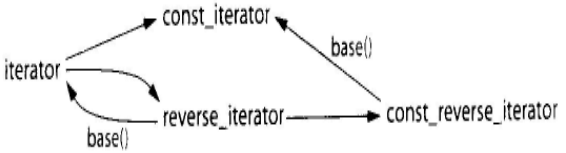
\includegraphics[width=0.6\linewidth]{pics/Iterators.png}
\end{center}
	\item Containers are required to provide iterator as a type convertible to const\_iterator, so you can convert implicitly:
\begin{lstlisting}	
Container::iterator it = /* blah */;
Container::const_iterator cit = it;	
\end{lstlisting}
			
	\item A good article is "effective modern C++" item 13. It introduce the basic idea about \texttt{const\_iterator.}
\end{itemize}

\subsection{constexpr}

\subsubsection{Basic definition}
\begin{itemize}
	
	\item The first conception is \textbf{const expressions}. constant expression is expression that can be evaluated at compile time. It has many advantage, such as can be performance optimization and can be used in places that require compile-time evaluation, for example, template parameters and array-size specifiers.
\begin{lstlisting}
int n = 1;            //n is not a constant expression
std::array<int, n> a1; //ERROR 
const int cn = 2;     // cn is a constant expression
std::array<int, cn> a2;// OK 
\end{lstlisting}
	
	\item After C++11, by introducing \texttt{constexpr} specifier, we expand the constant expression scope. For example, a constexpr function with known parameter can be constant expression too. \textbf{That is the basic idea of constexpr, If you understand this, you can understand a lot of complex syntactic knowledge below.}
	\begin{figure}[h]
		\centering
		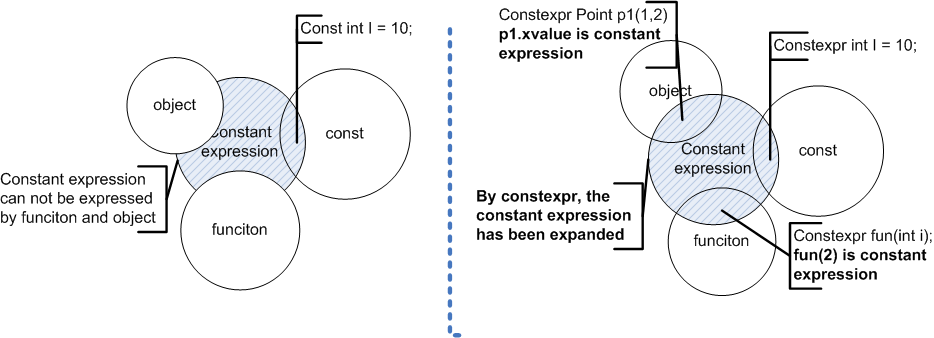
\includegraphics[width=0.9\linewidth]{pics/constexpr.png}
		\caption{Basic idea of constexpr}
		\label{fig:constexpr}
	\end{figure}
	
	\item The \textbf{constexpr specifier} declares that it is possible to evaluate the value of the function or variable at compile time. Such variables and functions can then be used where only compile time \textbf{constant expressions} are allowed (provided that appropriate function arguments are given). It has two advantages: 1) Improving efficiencies(if it's possible, it will calculate at compile time, not run time). 2) Expanding usage scope (initialize constexpr obj and use in integer constexpr context)
\begin{lstlisting}[frame=single, language=c++]
constexpr int fun(int a, int b){return a+b;}
	
constexpr int const foo = fun(2,3) ;  // without line 1 declaration, 
int a[fun(2,3)];                    //we can't use this way in line 3 and 4.
\end{lstlisting}
		
	
	\item \texttt{constexpr} can be used in three places: 
	\begin{enumerate}
		\item constexpr variable.
		\item constexpr obj.
		\item constexpr function. constexpr function can be thought as a kind of "metafunction".
	\end{enumerate}
	
	
	\item Difference between constant expression and \texttt{constexpr}:
	\begin{enumerate}
		\item Declaring a function as constexpr does not necessarily guarantee that it will be evaluated at compile time. It can be used for such, but it can be used in other places that are evaluated at run-time, as well.
		
		\item An object may be fit for use in constant expressions without being declared constexpr. for example: \texttt{const int N = 25}.
	\end{enumerate}
	
	\item Difference between \texttt{constexpr} with \texttt{const}:
	\begin{enumerate}
		\item when you declare \texttt{constexpr} obj, it implicit \texttt{const.} But not all \texttt{const} is \texttt{constexpr.}
		
		\item \texttt{constexpr} just used on top level. If you want to specify the low level \texttt{const,} you need to write it out.
\begin{lstlisting}
constexpr int const foo = 42;
constexpr int       foo = 42; //line 1 and 2 are same 
constexpr int const *pb = &bar; 
\end{lstlisting}
		\begin{description}
			\item[Line 3:] \texttt{pb} itself is constexpr, when we initialize it, \texttt{\&bar} must be constant expression too.
			\item[Line 3:] \texttt{pb} points const int, it means that we can't use \texttt{pb} to change \texttt{bar}.
		\end{description}
	\end{enumerate}
	
\end{itemize}


\subsubsection{constexpr variable and object}
\begin{itemize}
	\item \textbf{All constexpr objects are const, but not all const object are constexpr}
	\begin{enumerate}
		\item constexpr variable is implicitly const. Just like const, constexpr can't be changed during run time.
		
		\item constexpr variable must be initilized when you declare it. The full-expression of its initialization, including all implicit conversions, constructors calls, etc, must be a constant expression.(You know the exact value in compiling time.)
		
		\item Value of constexpr \textbf{must be known at compile time}.If you want to get value from a function, you have to use constexpr function to assign value to it. 
		
\begin{lstlisting}
constexpr int sum(int i, int j){
	return i+j;
}
int i,j;
cin>>i>>j;
const int result = i+j; //OK
const int ce = sum(i,j); //OK
constexpr int result = i+j;  //ERROR, can't calculate in compile time
constexpr ce = sum(i,j); //ERROR
\end{lstlisting}		
	\end{enumerate}
	
	\item For constexpr object, it must has corresponding  constexpr constructor. constructor body should be empty. You can't define constexpr object if the class has no constexpr constructor.
	\begin{enumerate}
		\item can only be invoked with constant expressions.
		\item can not use exception handling.
		\item has to be declared as default or delete or the function body must be empty (C++11).
		\item The constexpr user-defined type
	\end{enumerate}
	
	\item For class itself, it also need satisfy below:
	\begin{enumerate}
		\item can not have virtual base classes.
		\item requires that each base object and each non-static member has to be initialized in the initialization list of the constructor or directly in the class body. 
		\item Consequently, it holds that each used constructor (e.g of a base class) has to be constexpr constructor and that the applied initializers have to be constant expressions.
	\end{enumerate}
	
\begin{lstlisting}[frame=single, language=c++]
class MyInt{
	public:
	constexpr MyInt()= default;
	constexpr MyInt(int fir, int sec): myVal1(fir), myVal2(sec){}
	MyInt(int i){ myVal1= i-2; myVal2= i+3; }
    constexpr int getSum() const {return ...}
	
	private:
	int myVal1= 1998;
	int myVal2= 2003;
};

constexpr MyInt myIntConst1;
MyInt myInt2;
constexpr int sec= 2014;
constexpr MyInt myIntConst3(2011,sec);
int arr[myIntConst3.getSum()];
static_assert( myIntConst3.getSum() == 4025, "2011+014 = 4025" );
constexpr MyInt myIntConst5(2000); //Error, constructor is not declared as constexpr function
\end{lstlisting}
	\begin{description}

        \item[Line 6:] \textbf{A constexpr class must have a constexpr constructor. If a member function needs to be used in constexpr statement, it must be constexpr too: Note, in the member function definition, the qualifier of this must be const.}

		\item[Line 13 and 14:] You can declare both constexpr and non-constexpr object.
		
		\item[Line 15 and 16:] If you want to use constexpr to initialize constexpr variable, you must guarantee all the parameter are constexpr.
		
	\end{description}

	\item A good articles is: \\ \verb|https://www.modernescpp.com/index.php/constexpr-variables-and-objects|
\end{itemize}

\subsubsection{constexpr function}
\begin{itemize}
	\item  \texttt{Constexpr} can be used with both member and non-member functions, as well as constructors. It declares the function fit for use in constant expressions. \textbf{When you declare a function as constexpr, you just tell the compiler that this function is a kind of "pure function".} The pure function has no state, and when you run it, it has no side effect. 
	\begin{enumerate}
		\item The return value is only determined by its input values.
		\item Given input values, the return value can be calculated in compiling time. 
	\end{enumerate}
	
	
	\item The pure function has some advantages compared with ordinary funciton: Return always the same result when given the same arguments, So the function call can be replaced by the result, and the order of function call is not important.(That is why you can run it at compiling time.) But the problem is compiler itself can't judge if a function is pure function, That's why programmer come to rescue. The programmer indicate this function is a "pure" function, so compiler can \textbf{For outside} use it in another constant expression context, \textbf{For inside} calculate it in compiling time. 
	
	\item On the first sight, you should declare constexpr function everywhere, but it's not good idea either. That makes a constexpr qualifier an irrevocable design decision. You cannot remove this qualifier without an incompatible change to your API. It also limits how you can implement that function, e.g. you would not be able to do any logging within this function. Not every trivial function will stay trivial in eternity. That means you should preferably use constexpr for functions that are \textbf{inherently pure functions}, and that would be actually \textbf{useful at compile time} (e.g. for template metaprogramming). It would not be good to make functions constexpr just because the current implementation happens to be constexpr-able. In semantic level, you should have something that can be evaluated down to a constant while maintaining good readability and allowing slightly more complex processing than just setting a constant to a number. Take \texttt{max( a, b )} for example: Its a pretty simple choice there but it does mean that if you call max with constant values it is explicitly calculated at compile time and not at run time.
\begin{lstlisting}[numbers=none]
constexpr int MeaningOfLife ( int a, int b ) { return a * b; }
constexpr int meaningOfLife = MeaningOfLife( 6, 7 );
	
template< typename Type > 
constexpr Type max(Type a, Type b) {return a < b ? b : a; }
\end{lstlisting}		
		
	\item constexpr functions compile much quicker than the equivalent template-based solutions, which scale linearly with the depth of the template-recursion. Where compile-time evaluation is not necessary, using inline functions or functions with internal linkage would seem more appropriate than constexpr. Both constexpr and inline are for performance improvements, inline functions are request to compiler to expand at compile time and save time of function call overheads. In inline functions, expressions are always evaluated at run time. constexpr is different, here expressions are evaluated at compile time.

	
	\item Compared with ordinary function, constexpr functions:
	\begin{enumerate}
		\item \textbf{For outside}. is able to be used in the another constant expression(such as \texttt{constexpr int sum = cfun(2,3);} ) But it doesn't mean that it must be used in constant expression(such as \texttt{int sum = cfun(i,j);})
		
		
		\item \textbf{For inside}. constexpr function adds a lot of constraints on its implementation.
	\end{enumerate}
	
\begin{lstlisting}[frame=single, language=c++]
constexpr int cfun(int i, int j){
	return i+j;
}
int fun(int i, int j){
	return i+j;
}

int i, j;
constexpr int sum = fun(2,3);  //Error
constexpr int sum = fun(i,j);  //Error
constexpr int sum = cfun(2,3); //OK
constexpr int sum = cfun(i,j); //Error

int sum = fun(2,3);  //OK
int sum = fun(i,j);  //OK
int sum = cfun(2,3); //OK
int sum = cfun(i,j); //OK
\end{lstlisting}
	
	\begin{description}
		\item[Line 9 to 12:] For constexpr variable, only cfun with constant expression is OK.
		\item[Line 14 to 17:] For Non-constexpr variable, all fun is OK.
	\end{description}
	
	\item Even with constexpr paramter, constexpr function doesn't guarantee to be evaluated at compile time. There are three contexts in which a constexpr function \textbf{MUST} to run at compile time. That's why constexpr functions must be able to return compile-time results when called with compile-time values.

	\begin{enumerate}
		\item The constexpr function is executed in a context which is evaluated at compile time. This can be a \texttt{static\_assert} expression such as with the type-traits library or the initialisation of a C-array.
		
		\item The value of a constexpr function is requested during compile time with constexpr: \texttt{constexpr auto res = func(5);}
		
		\item a template parameter or enum or switch statement.
	\end{enumerate}
	
	\item In C++11. For constexpr functions there are a few restrictions on it: it has to be non-virtual. It has to have arguments and a return value of a literal type. Literal types are the types of constexpr variables.The function body must be extremely simple: Apart from typedefs and static asserts, only a single return statement is allowed. In the case of a constructor, only an initialization list, typedefs and static assert are allowed. (= default and = delete are allowed, too, though.)
	
\begin{lstlisting}[frame=single, language=c++]
constexpr int gcd(int a, int b){
	return (b== 0) ? a : gcd(b, a % b);
}  //use ternary to replace if
\end{lstlisting}
	
	\item In C++14. constexpr function can include: conditional jump instructions or loop instructions and more than one instruction. fundamental data types that have to be initialized with a constant expression.The arguments and the return type must be \textbf{literal types} (i.e., generally speaking, very simple types, typically scalars or aggregates)
		
\begin{lstlisting}[numbers=none]
constexpr auto gcd(int a, int b){
	while (b != 0){
		auto t= b;
		b= a % b;
		a= t;
	}
	return a;
}
\end{lstlisting}
    \item A literal type is a type that can qualify as constexpr. This is true for scalar types, references, certain classes, and arrays of any such types. A class that is a literal type is a class (defined with class, struct or union) that has a trivial destructor. And every constructor call and any non-static data member that has brace- or equal- initializers is a constant expression, is an aggregate type, or has at least one constexpr constructor or constructor template that is not a copy or move constructor. It has all non-static data members and base classes of literal types 
\begin{lstlisting}[]
struct A { };
struct B { ~B(){} };

cout << is_literal_type<int>::value ; //int& and int* and A true
cout << "B: " << is_literal_type<B>::value;  //Only this line print false

struct point {
	point(): x(0), y(0){  std::cout << "point() called" << std::endl; }
	constexpr point(int x_, int y_): x(x_),y(y_){}
	constexpr int hypot() { return x*x + y*y; }
private:
int x,y;
};

static_assert( point(3,4).hypot() == 25 );
std::cout << "std::is_literal_type<point>::value=" << std::is_literal_type<point>::value;
\end{lstlisting}
	
	\item \textbf{Use constexpr, const and noexcept more aggressively.} This adds more compilation-time checks, gives the compiler more information to optimize better and this has the nice side effect of making you think more about what you are currently doing. And remember: the longer it takes for your C++ program to compile, the greater your eliteness.

	\item A good artical is "Demystifying constexpr". 
\end{itemize}

\subsection{static}
\begin{itemize}
	\item In C++, \textbf{global and static variables initialized to default values.}  But auto variable is random value, unless you use value initialization, because of efficiency consideration. 
	
	\item You can't initialize a static member variable inside the class declaration, you need to put it in a .cpp file.   But you can if the static data member is \texttt{const} of integer or enumeration. If you have a const member inside a class, better to use \texttt{const static}, because it can't be changed, so all the object can share the same static value.
\begin{lstlisting}[frame=single, language=c++]
class{  //in .h file
	static int obj_num;  // you can't initialize
	const static int months = 12; // you can initialize inside the class
};

int class::obj_num = 12; //in .cpp, no static keyword anymore.	
                     //will be 0 if you don't initialize it.
\end{lstlisting}	
	
	\item static member function has two usages:
	\begin{enumerate}
		\item It can be invoked just by class name, not object instance, so you can define math class and define a lot static math function inside it.  Just like namespace.
		
		\item It can't access class data member, only can access class static member data. Because for static function, we don't pass \texttt(this) pointer.
	\end{enumerate}
	
	\item static can be used restrict the scope.(internal linkage)
\begin{lstlisting}[frame=single, language=c++]
int global = 0;  //All files
static int s_i = 50; //just in this file
main(){
	static int s_i = 100;  //just in this block
	printf("%d %d", ::s_i, s_i); //print 50 and 100
}
\end{lstlisting}
	\begin{description}
		
		\item[Line 5:] Not conflict, but if you define int \texttt{s\_i} in global scope it will conflict.
		
		\item after C++ 11, static variable inside a function is thread safe, so it's an important improvement for singleton patten.
		
	\end{description}
	
	\item Summary: Use \texttt{static} in three ways:
	\begin{enumerate}
		\item Use it inside a function. invisible outside of function, static life time and valid until program end.
		
		\item Use it inside a class. only copy for all instances, and access by static member function.
		
		\item Use it inside a file. internal link, avoid name conflict. But by now, we prefer to use unnamed namespace in modern C++.
	\end{enumerate}
\end{itemize}


\section{Complex declaration}

\begin{itemize}	
	\item pointer to pointer is used mostly in ragged array, array of list. For ragged char array, use null character as end, for ragged int array, you need extra size information. If you want to modify pointer parameter, you can use \texttt{int* \&p}; It's more clear and direct than useing pointer to pointer. 
\begin{lstlisting}
int** p = new int* [2];
p[0] = new int[2];
p[1] = new int[3];
p[0][1] = 0;

int* &rp = p[0]; 

delete [] p[0];
delete [] p[1];
delete [] p;		
\end{lstlisting}
	
		\item Any complex declaration is either a pointer to an array or a pointer to a function. Let me introduce pointer to an array first. 
\begin{lstlisting}
int a [2] = {1, 3};
int b [3] = {1, 2, 3};

int (*p)[] ; //can omit the dimension, but you can not increment it.
p = &b; //p = &a is OK, (*p)[1] is ok, but ++p error

int (*p)[3]; //C/C++ both support int(*p)[] and int(*p)[3]
p = &b; //p = &a is error, (*p)[1] is ok, but ++p is OK.
\end{lstlisting}
	
	\item Usage of \texttt{typedef}. When you use typedef, the basic sytax is the same, but the identifier has become a type, not variable. Usually, we use capital letter to denote that it's a type.
\begin{lstlisting}[]
struct Block{
	int i;
	int j;
} bb;  //define variable, bb is variable.

typedef struct Block{
	int i;
	int j;
} BB;  //define type, BB is type 
\end{lstlisting}
	
	\item pointer to function. You can use \texttt{typedef} to help you to define a pointer to function.
\begin{lstlisting}
int (*foo_ptr)( int )

typedef int (*FOO_PTR_T)( int );
FOO_PTR_T foo_ptr;
\end{lstlisting}
	
	\item A array of pointer to function. From below, you can see the advantage of using \texttt{typedef}.
\begin{lstlisting}
int (*foo_ptr_array[2])( int )

typedef int (*Foo_ptr_t)( int ); //A better way is to use typedef
Foo_ptr_t foo_ptr_array[2];
\end{lstlisting}
	\begin{description}
		\item[1] The first step, get the variable name, look right, found that it's array. what types are in the array?
		\item[2] Then look left, found that pointer, then that is an array pointer.
		\item[3] Then look right, found that this is parentheses, that is function. so pointer to function, what type of function?
		\item[4] then look left, paramter is \texttt{int}, and return type is \texttt{int} too.
	\end{description}
	
	\item pointer to function which return complex type. This is a function pointer, The function input a \texttt{int} and return a pointer. The reture pointer points to an array, and array's element type is \texttt{int *}.
\begin{lstlisting}
int * (* (*fp1) (int) ) [10];

//Start from the variable name -> fp1
//Nothing to right but ) so go left to find * -> is a pointer
//Jump out of parentheses and encounter (int) -> to a function that takes an int as argument
//Go left, find * -> and returns a pointer
//Jump put of parentheses, go right and hit [10] -> to an array of 10
//Go left find * -> pointers to
//Go left again, find int -> ints.
\end{lstlisting}
	\item \textbf{The basic method is find the identifier name, then use it as center point to expand to both side following right-then-left rule.} A good reference is here: How to interpret complex C/C++ declarations. You can google and read it. 	
\end{itemize}

\section{Name}
\subsection{Namespace}

\begin{itemize}
	\item Don't put a lot of stuff in global-scope, learn to using namespace to split your global-scope into different scopes. If you develop a library of functions or classes, you should put them in a new namespace, just like std namespace in STL. Don't put your own class into namespace \texttt{std}; Usually, namespace should be your project name, you can add company name in front of it if you like.
		
	\item Use \texttt{::} before function will means that global namespace, For example, \texttt{::max} will hide \texttt{std::max}, in this way, you can define your own max function in global scope, and use \texttt{::max} call your own max function. 
	
	\item \textbf{Namespaces can be located at the global level or inside other namespaces. They can't be placed in a block.} So it has external linkage by default, that is to say it can be accessed by multi translation unit(files).


	\item There are three kinds of namespace usages. Using-declaration introduces a member of another namespace into current namespace or block scope. It's the recommended way to use namespace. 
\begin{lstlisting}[numbers = none]
using sp::name;   //1) using declaration
using namespace sp;   //2) using directive
sp::name   //3) specific refer it
	
namespace ns{
	int zy;
}
using std::string; //using declaration
using namespace ns;
int main(){
	string str = "abc" //don't need to use std::string.
	int zy = 0; //it will hide ns::zy
	cin>>zy; //read into local zy
}
\end{lstlisting}

	\item Suggestions about "using directive".
\begin{enumerate}
	\item  \textbf{Don't use using directive in any .h file,  because It will "pollute" all the .cpp file which include this head file.}
	
	\item Use using directive as little as possible in any .cpp file, you should using scope-resolution or using declaration more. It will avoid polluting namespace.
\begin{lstlisting}[numbers=none]
#include <iostream>
using std::cout;
using std::endl;

int main(){
	cout<<"Hello world"<<endl;
}	
\end{lstlisting}	
	
	\item If you \textbf{have to} use using directive in your .cpp file, put it after all the include files.

		\end{enumerate}
	
	\item For implementation code, there are four methods to put it into namespace. Method 3 and method 4 are recommended.
	
\begin{lstlisting}[frame=single, language=c++]
namespace Yan{ //a.h
	Class Foo{
		void mem_fun();
	};
}
	
using Yan::Foo;  //method 1. using declaration
void Foo::mem_fun(){.......}
	
using namespace Yan; //method 2. using directive. It's bad style.
void Foo::mem_fun(){.........}
	
void Yan::Foo::mem_fun(){.........} //method 3. It's good style.

namespace Yan{  //method 4. can include more contents in side.
	void Foo::mem_fun(){......}
}
\end{lstlisting}

	
	
	\item unnamed namespace just like \texttt{static} to specify its content to local file scope. At the same time, make anonymous namespace as small as possible.  see C++ primer p492.
	
\begin{lstlisting}[numbers=none]
// a.cpp file
static int count;

namespace{ // A better method to use namespace.
	int count;
}
\end{lstlisting}
	
\end{itemize}


\subsection{Name lookup}
\begin{itemize}
	
	\item \textbf{Phases of the function call has three steps, they are:} 1) Name lookup. 2) Overload resolution. and 3) Access control.
	
	\item Detail explanation is below:
	\begin{enumerate}
		\item First, compiler looks in the \textbf{immediate scope},  and makes a list of all functions that have right names  (regardless of whether they're accessible or even take the right number of parameters). Please note, \textbf{If compiler has found function name, even the parameters don't match, compiler will not continue outward search. It stops here and barks}. It's a safe measure, compiler think the immediate scope is "priority zone". Maybe you omit parameter, compiler should not search outward implicitly. 
		
		\item Only if compiler doesn't find any same function name at all, then compiler continue to "search outward" into the next enclosing scope and repeat.
		
		\item In the searching scope, if there are more than one candidate functions, the compiler perform overload resolution and then applying access rules. \textbf{In one word, overload resolution does not go beyond scopes!}
	\end{enumerate}
	
	
	\item Overload resolution has a good introduction: "C++ Primer plus" chapter 8 "Which Function version the compiler pick". The main idea is: \textbf{exact match non-template > template > argument conversion(promotion or implicit conversion)}. Compiler will first match function name and number of arguments, then look for template deducted function, then use implicit conversion to try match. \textbf{So implicit conversion happens after template.}
\end{itemize}

\subsubsection{Name searching scope}
\begin{itemize}
	
	\item There are four examples about immediate scope.
	\begin{enumerate}
		\item class scope:
\begin{lstlisting}
void f1(int i ){...};

class Foo{
	void f1(string & str){};
	void f2(void){
		int i = 3;
		f1(i); //compiler bark here! it only see f1(string &)
	}
};
\end{lstlisting}
		
		\item Child class scope. 
\begin{lstlisting}
struct B{
	int f( int );
	int g( int );
};
		
struct D : public B{
private:
	int g( std::string, bool );
};
		
D d;
int i;
d.f(i); // ok, means B::f(int)
d.g(i); //error: g takes 2 args
\end{lstlisting}
\begin{description}
	\item[Line 14:] In child class scope, if it found name \texttt{g}, then it will stop looking for another name in outward scope. just use \texttt{g}, then found argument number is not match, then compiler barks.
\end{description}
		
\item Nested namespace scope. (global includes namespace N)
\begin{lstlisting}
void f1(int i ){...};

namespace N{
	void f1(string & str){};
	void f2(void){
		int i = 3;
		f1(i); //compiler will bark here! Use ::f1(i)to specify global one
	}
};
\end{lstlisting}

		\item Nested scope. A class name or enumeration name can be hidden by an explicit declaration of that same name -- as an object, function, or enumerator -- in a nested declarative region or derived class.
\begin{lstlisting}[numbers=none]
int x =2;
{
	int x = 3; 
	cout<<x; //output 3
}
\end{lstlisting}
		
	\end{enumerate}
	
	\item Overwrite is not standard conception in C++, most time, you can call it \textbf{name hiding}. There are two things: The first one is if you redefine the same name non-virtual function in both base and child classes, you can't use dynamic binding, just static binding. 
\begin{lstlisting}[frame=single, language=c++]
class A{
	f(int) {}
};
class B:public class A{
	f(int)  {} // overwrite A::f(int)
};
	
A* pa = new B();
pa->f(3) // call base f, because pa is A*, event it points to B. 
\end{lstlisting}

	
	\item How to expand searching scope?  There are two method:
	\begin{enumerate}
		\item using declaration to introduce name into the name lookup.
		
		\item You can use :: to specify global variable name or function if you have same name in you local scope.  Or use \texttt{Base::} to specify Base scope name if you have same name in derived class.
\begin{lstlisting}
struct B{
	int g( int );
};

struct D : public B{ 
	using B::g;  //mehtod 1: using declaration, can orverload later
	private:
	int g( std::string, bool );
};
D d; 
d.g(3) // also OK. 

struct D : public B{
private:
	int g( std::string, bool );
};
d.B::g(3);  // method 2: use scope specifier 
\end{lstlisting}
		
	\end{enumerate}

	\item  \textbf{Overloading just happens in the same name scope, not in the hierarchy}. So in this way, any same name is base class will not visible in derived class. You can use using declaration to add it in your derived class, then it will compile. Considering these complicated things, \textbf{Don't redefine or overload base class any non virtual functions in your child class.}

\end{itemize}

\subsubsection{ADL}
\begin{itemize}
	\item For a class X, all functions, including non member functions, that both "Mention" X and "supplied with" X are logically part of X, because they form part of the interface of X. supplied with X means that function is defined in the same .h file with type X. 
	
	\item Keep a type and its nonmember function interface in the same namespace, 1) in logic, these nonmember function can be regarded as type interface, 2) avoid name ambiguous problem in the future.
\begin{lstlisting}[numbers=none]
namespace N{
	class X {};
	X operator+( const X&, const X& );
}

x3 = x1+x2;	
\end{lstlisting}	
	
	\item On the contrary, put types and functions in separate namespaces unless they're specifically intended to work together.
	
\begin{lstlisting}[numbers=none]
#include <vector>
namespace N {
	struct X {};
}
// this template should not be put in the namespace N
template<typename T>
int* operator+( T , unsigned ) {/* do something */}	
\end{lstlisting}	
		
	\item Koenig, also called Argument-Dependent Lookup(ADL) lookup. If you supply a function argument of class type (here \texttt{parm} of type \texttt{NS::T}), then to look up the correct function name the compiler considers matching names in the namespace (here \texttt{NS}) containing the argument's type.
	
\begin{lstlisting}[numbers=none]
namespace NS{
	class T { };
	void f(T);
}
	
NS::T parm;
int main() {
	f(parm); // OK, Found NS::f by ADL, then calls NS::f
}
\end{lstlisting}

\item compiler applies ADL whenever it's doing name lookup (building a candidate set) for an unqualified function call. If the name of the thing-being-called has any :: qualification at all, then ADL won't kick in.

\begin{lstlisting}[numbers=none]
namespace A {
	struct A { operator int(); };
	void f(A);
}
namespace B {
	void f(int);
	void test() {
		A::A a;
		f(a);     // ADL, calls A::f(A)
		B::f(a);  // no ADL, calls B::f(int)
	}	
}
\end{lstlisting}

\item  If the thing is not "a function call," then ADL won't kick in. (Of course, we don't try to apply Argument-Dependent Lookup to names that don't have arguments.) 
	
\item ADL is for resolve \texttt{operator<<} problem.
\begin{lstlisting}[frame=single, language=c++]
namespace sak { // SakBigNum.h
	struct bignum {
		bignum operator++();
	};
	std::ostream& operator<<(std::ostream&, bignum); 
}

namespace ajo { // AjoBigNum.h
	struct bignum {
		bignum operator++();
	};
	std::ostream& operator<<(std::ostream&, bignum);
	void bar(int& x) {
		sak::bignum b;   // refers to sak::bignum
		++b;             // calls sak::bignum::operator++()
		std::cout << b; //ADL use here
	}
}
\end{lstlisting}
\begin{description}
	\item[Line 16:] UH-OH! We should call \texttt{operator <<} in line 5 in sak namespace. If there is not ADL, we call \texttt{operator <<} in ine 12, compiler will stop because we can't change \texttt{sak::bignum} to \texttt{ajo::bignum}.
\end{description}
	
	\item ADL can bring name lookup ambiguous problem.  When you call \texttt{f(parm)}, number 2 is in global scope, so it is in the \textbf{searching scope} default. But ADL bring namespace NS scope into searching scope, and there are two options now. Compiler will bark.
	
\begin{lstlisting}[numbers=none]
namespace NS { // some header T.h
	class T { };
	void f( T ); //  number 1, add new function
}
void f( NS::T ); //number 2	
int main(){
	NS::T parm;
	f(parm); // ambiguous: NS::f  or global f?
}
\end{lstlisting}
	
	
	\item In name lookup, the C++ language deliberately says that a member function is to be considered more strongly related to a class than a nonmember.
\begin{lstlisting}[numbers=none]
namespace A{
	class X { };
	void f( X );
}
	
class B{ // <-- class, not namespace
	void f( A::X );
	void g( A::X parm ){
		f(parm); // OK: B::f, not ambiguous, event ADL bring in f in namespace A.
	}
};
\end{lstlisting}
	
\end{itemize}


\section{operator and operator overload}

\begin{itemize}
	\item For operator, there are two important characteristics: \textbf{Precedence} and \textbf{Associativity}. Below example explains associativity. \textbf{When operators have the same precedence, then associativity will kick in to decide which step need to be preform first.}
	
\begin{lstlisting}
a=b=c; //correct code
a<b<c; //ERROR code
a<b && b<c //correct code

int a, b = 1, c = 2
a=b=c //Why associativity is important? for this statement, 
      //left to right or right to left will give two differents answers. 
\end{lstlisting}

\begin{description}
	\item[Line 1:] assignment operator's associativity is \textbf{right-to-left}. It means that we 1)\texttt{b=c}, 2)\texttt{b=c} yields \texttt{b} 3) \texttt{a=b} 
	
	\item[Line 2:] logical operator's associativity is \textbf{left-to-right}. it means that 1)\texttt{a<b}, 2)\texttt{a<b} yields bool value 3) \texttt{bool<c}. The code can be compiled successfuly, but the semantic is wrong and is not what you expect.  
\end{description}

    \item Most of operators are right-to-left associativity, there are major two groups of operators which are right-to-left associativity, each group has the same precedence.

\begin{tabular}{|p{0.3\textwidth}|p{0.1\textwidth}|p{0.3\textwidth}|p{0.1\textwidth}|}
	\tophline
    Prefix increment & ++ & Prefix decrement & --\\
	\tophline
    bit complement & \~{} & logic not & ! \\
	\tophline
    address & \& & indirection & * \\
	\tophline
    unary negation & - & Unary plus & +
	\bottomhline
\end{tabular} \\
These operators have very high precedence(group 3), Another low precedence group operators(group 15) is right-to-left associativity too. They are assignment(=) and various combined assignment(+=, -=,..).

	\item \textbf{Prefer Preincrement (++i), especially in a for loop.}  When you use ++i or i++ inside expression, there are differences. Otherwise, there is no differences.
	
\begin{lstlisting}[numbers=none]
for(int i = 0;i<10; ++i)
j=++i; // j = i+1;
j=i++; //j = i;  i=i+1;
++*p;  //++(*p) ; prefix ++ and * has same precedence,  both right to left
*++p; //*(++p);
\end{lstlisting}
	
	\item How to understand \texttt{*p++} ? Prefix and postfix are both syntax sugar, in order to reduce typing.   But prefix represents \textbf{one statement}, postfix means \textbf{two statements}. Precedence of postfix \texttt{++} is higher than both \texttt{*} and prefix \texttt{++}. Associativity of postfix \texttt{++} is left to right.
\begin{lstlisting}[frame=single, language=c++]
++i;  //just like i = i+1 or  i+=1;
*p++; // *(p++);  *p ; p=p+1;

while(*p != '\0'){
	p= p+1;
}
//can be written to
while(*p++ != '\0')	
\end{lstlisting}		

	\item Overload means providing two (or more) functions that perform similar, closely related things, differentiated by the types and/or number of arguments it accepts.
	
	\begin{enumerate}
		\item \textbf{In some cases it's worth arguing that a function of a different name is a better choice than an overloaded function.}
		
		\item  In the case of constructors and operator, overloading is the only choice because we can't give them the different name. and operator overload is typical feature in Object Base Programming.(OB)
		
		\item Sometimes, overload and default parameter have same client usage, as shown below. If there is a value that you can use for a default, use default parameter. Overload usually take different parameter type or different number of parameters.
\begin{lstlisting}[numbers=none]
void f();
void f(int x);
f() or f(10);

void g(int x = 0);
g() or g(10);
\end{lstlisting}		
	\end{enumerate}
	
	\item Overloading sometimes can help you to avoid implicit type conversion. In the below example, we avoid creating a temporary obj implicitly created by constructor.
	
\begin{lstlisting}[frame=single, language=c++]
class String{
	bool operator==(const String& lhs, const String& rhs);
}
String str;
if(str =="hello") //will build a temp obj String("hello");
	
bool operator==(const String& lhs, const char* rhs);  //avoid implicit type conversion.
\end{lstlisting}

	\item The binary operators = (assignment), [] (array subscription), -> (member access), as well as the unary () (function call) operator, must always be implemented as member functions, because the syntax of the language requires them to.
	
	\item Other operators can be implemented either as members or as non-members. Some of them, however, usually have to be implemented as non-member functions, because their left operand cannot be modified by you. The most prominent of these are the input and output operators \texttt{<<} and \texttt{>>}, whose left operands are stream classes from the standard library which you cannot change.
	
	\item For all operators where you have to choose to either implement them as a member function or a non-member function, use the following rules of thumb to decide:
	\begin{enumerate}
		\item If it is a unary operator, implement it as a member function.
		
		\item If a binary operator treats both operands equally (it leaves them unchanged), implement this operator as a non-member function.
		
		\item If a binary operator does not treat both of its operands equally (usually it will change its left operand), it might be useful to make it a member function of its left operand’s type, if it has to access the operand's private parts.
	\end{enumerate}
	
\end{itemize}

\chapter{Initialization}
\section{Basic knowledge}

\subsection{Basic principles and terminology}
\begin{itemize}
	\item \textbf{Always initialize variable before you use it.} Manually initialize any non-member objects of built-in types, including a pointer.
	
	\item There are three names you need to distinguish: 1)initilizer list, 2) braces(uniform) initialization, 3) member initialization list(mem-init)

	\begin{enumerate}
		\item Member initialization list is used in C++ constructor to initialize all members inside an object. it has some advantages: Detail can be found in "OOP" chapter. For example, reference type member variable can only be initialized by member initialization list. It also has higher efficiency. (just call copy constructor once) 
		
		\item Braces initialization is a generic initialization syntax(method), it supports a kind of uniform initialization, such as class member and aggregation. At the same time, it avoids narrowing and vexing parsing problem. 
		
		\item Initilizer list is \texttt{std::initializer\_list}. It is a \textbf{new data type. just like std::list.}
	\end{enumerate}

	\item Constructor with one parameter is called converting constructor. After C++ 11, A constructor that is not declared with the specifier explicit is called a converting constructor. please note here, Implicitly-declared and user-defined non-explicit copy constructors and move constructors are all converting constructors after c++ 11. Why are constructors with more than a single parameter considered to be \textbf{converting constructors} after C++11? That is because the new standard provides us with some handy syntax for passing arguments and returning values using braced-init-lists. Consider the following example: The ability to specify the return value as a braced-init-list is considered to be a conversion. This uses the converting constructor for foo that takes a float and an int. In addition, we can call this function by doing bar(\{2.5f, 10\}). \textbf{Converting only cares about if it has explicit, if there is no explicit, even zeor or more than 1 parameter are in consturctor, it is still converting constructor.} 

\begin{lstlisting}[numbers=none]
struct Foo{
	Foo() { }         // converting constructor (since C++11)  
	Foo(int) { }      // converting constructor
	Foo(float, int) { } // converting constructor (since C++11)
};
Foo bar(Foo f) {
	return {1.0f, 5}; //CONVERTING two numbers into Foo.
}
\end{lstlisting}	

	\item The \textbf{uniform initialization} is a feature that permits the usage of a consistent syntax to initialize variables and objects which are ranging from primitive type to aggregates. In other words, it introduces \textbf{brace-initialization} that applies braces (\{\}) to enclose initializer values.
	
	\item \textbf{List initialization} is comprised of direct-list-initialization and copy-list-initialization. It's concrete initialize method. \textbf{brace-initialization} is generic conception. In this book, uniform(brace) or list initialization are interchangeable. 
	
	\item default constructor is different with default initialization. copy constructor is also different with copy initialization.
	
	\item A good reference page is \verb|https://en.cppreference.com/w/cpp/language/initialization|. Anytime you have question, you can go to there to get the official explanation. 
\end{itemize}

\subsection{static initialization and dynamic initialization}
\begin{itemize}
	\item In the same translation unit, formally, C++ initializes static and global variables in this order:
	\begin{enumerate}
		\item Static initialization.
			\begin{enumerate}
			\item Zero initialization.
			\item Const initialization.
			\end{enumerate}
		\item Dynamic initialization.
	\end{enumerate}
		
\begin{lstlisting}[numbers=none]
int g0;  //zero initialization
int g1 = 42;    //  constant initialization
extern int f();
int g2 = f();   //  dynamic initialization
\end{lstlisting}

	\item You can see the dynamic initialization happen after static initialization. Sometimes it causes some subtle bugs shown below:
\begin{lstlisting}[frame=single, language=c++, mathescape=true]
int a = f(); // call f first
int x = 22; //this line call first.
int f() {
	++x;
	return 123; // unimportant arbitrary number
} //x equals to 23, not 22. because static init is earlier than dynamic
\end{lstlisting}

	
	\item Pay attention to the global object which are initialized in right order. Because the order can be arranged in the same translation unit, but not \textbf{between translation units}, see effective c++ Item 47. The initialization order uncertainty in separate translation units can cause below problem.
	
\begin{lstlisting}[frame=single, language=c++]
#include "x.h" // File x.cpp
X x;    //x maybe initialize before y or after y.
	
#include "y.h" // File y.cpp
extern X x;
Y y;
Y::Y(){ 
	x.goBowling(); //Here x maybe not be constructed
}
\end{lstlisting}
	
	\item  How to resolve? 1)We don't encourage you to use global object unless it's very necessary. 2)Using a singleton design pattern.
	\begin{lstlisting}[numbers=none]
#include "x.h"  // File x.cpp
X& getX(){
	static X x;   //static X* px = new X();
	return x;     //return *px
}
	
#include "y.h" // File y.cpp
Y y;
Y::Y(){
	getX().goBowling();
}
\end{lstlisting}
\end{itemize}


\subsection{Initialization  categories}

\subsubsection{Six kinds of initialization}
\begin{itemize}
	\item There are six \textbf{initialization methods}:
	\begin{enumerate}
		\item Default initialization syntax and example. Two points to clarify: 1) default initialization doesn't equal calling default constructor. 2) default initializaiton doesn't means to set variable to zeor. Default initialization call default constructor or does nothing. If it doesn't nothing, it produces indeterminate value.
\begin{lstlisting}[numbers=none]
T t;
new T;  //default
\end{lstlisting}

	
\begin{lstlisting}
struct T1 { int mem; };
struct T2{
	int mem;
	T2() { } // "mem" is not in the initializer list
};
int n; // static non-class, a two-phase initialization is done:
	// first, zero initialization, then default initialization does nothing
	
int main(){
	int n;          // non-class, the value is indeterminate
	std::string s;  // class, calls default constructor, s is "" (empty string)
	std::string a[2]; // array, default-initializes the elements, a is {"", ""}
	//  int& r;       // error: a reference
	//  const int n;  // error: a const non-class
	//  const T1 t1;  // error: const class with implicit default constructor
	T1 t1;            // class, calls implicit default constructor
	const T2 t2;   // const class, calls the user-provided default constructor
                  // t2.mem is default-initialized (to indeterminate value)
}
\end{lstlisting}

\begin{description}
	\item[Line 8:] static initialization and default initialization is not exclusive each other, they can be combined. 
\end{description}


		\item Value initialization syntax and example.
\begin{lstlisting}[numbers=none]
T(); T{};
new T(); new T{};
Class::Class(...): member(), member{} {...} 
// class member initializer lists (value Init)
\end{lstlisting}


\begin{lstlisting}
struct T1{
	int mem1;
	std::string mem2;
}; // implicit default constructor

struct T2{
	int mem1;
	std::string mem2;
	T2(const T2&) { } // user-provided copy constructor, no default ctor
};

struct T3{
	int mem1;
	std::string mem2;
	T3() { } // user-provided default constructor
};
std::string s{}; // class => default-initialization, the value is ""

int n{};                // scalar => zero-initialization, the value is 0
double f = double();    // scalar => zero-initialization, the value is 0.0
int* a = new int[10](); // array => value-initialization of each element 0

T1 t1{};		// class with implicit default constructor =>
// t1.mem1 is zero-initialized 0, t1.mem2 is default-initialized ""

//  T2 t2{};	// error: class with no default constructor

T3 t3{};		// class with user-provided default constructor =>
// t3.mem1 is default-init to indeterminate, t3.mem2 is default-init ""

std::vector<int> v(3);  // value-initialization of each element to 0
\end{lstlisting}


		\item Direct initialization syntax and example
\begin{lstlisting}[numbers=none]
T object(arg, ... );
T(arg1, arg2, ... );
new T(args, ...)
: member(args, ...)   // class member initializer lists
T(other)              // function-style cast
static_cast<T>(other) // explicit static_cast
[arg](){...}          // lambda closure arguments captured by value
					//lambda is object, so for this object, 
					//lambda_1 obj(arg), is a direct init
\end{lstlisting}


\begin{lstlisting}[numbers=none]
struct Foo {
	int mem;
	explicit Foo(int n) : mem(n) {}
};

Foo f(2); // f is direct-initialized:
Foo f2 = 2; //error, because constructor is explicit.
\end{lstlisting}


		\item Copy initialization syntax and example.
\begin{lstlisting}[numbers=none]
T object = other;     // Initialization via assignment
T array[N] = {other}; // In array-initialization, the individual value are copy-init
f(other)                 // Pass-by-value
return other;            // Return-by-value
catch (T object)         // Catch-by-value
throw object;
\end{lstlisting}

\begin{lstlisting}[]
struct A {
	operator int() { return 12;}
};

struct B {
	B(int) {}
};

int c = b; // this is also copy initialization. 
A a;
//B b1 = a;  // it's copy initialization, but fail. 
B b2{a};     // calling A::operator int(), then B::B(int)
B b3 = {a};  //like line 12. not copy initialization, but list initialization.
auto b4 = B{a}; //like line 12. not copy initialization, but direct init.
\end{lstlisting}

		\item Aggregate initialization is used when initializing arrays or simple struct (all-member-public, no user-provided c'ctors.)
\begin{lstlisting}[numbers=none]
T object = {arg1, arg2, ...}; // If T is an array or a simple struct
T object{arg1, arg2, ...};    // If T is an array or a simple struct
\end{lstlisting}

\begin{lstlisting}[numbers=none]
struct S {
	int x;
	struct Foo {
		int i;
		int j;
		int a[3];
	} b;
};

S s1 = { 1, { 2, 3, {4, 5, 6} } };
S s2 = { 1, 2, 3, 4, 5, 6}; // same, but with brace elision
S s3{1, {2, 3, {4, 5, 6} } }; // using direct-list-initialization syntax
S s4{1, 2, 3, 4, 5, 6}; // error until CWG 1270: 
						// brace elision only allowed with equals sign
\end{lstlisting}

		\item reference initialization. It must has a reference symbol.
\begin{lstlisting}[numbers=none]
T & ref = object ;
T & ref = { arg1, arg2, ... };
T & ref ( object ) ;
T & ref { arg1, arg2, ... } ;
\end{lstlisting}
	\end{enumerate}

    \item You can use brace elision in the aggregate initilization.
\begin{lstlisting}
struct A{
	int foo;
	double bar;
};
struct Aarray{
	A data[2];  //data is an internal array
};
int main() {
	array<int, 5> a{1,2,3,4,5};  // without =, no nested aggregated, brace elision is also ok.
	
	Aarray a1 {
		{  //<--this tells the compiler that initialization of `data` starts
			{ //<-- initialization of `data[0]` starts
				0, 0.1
			}, //<-- initialization of `data[0]` ends
			
			{2, 3.4}  //initialization of data[1] starts and ends, as above
		} //<--this tells the compiler that initialization of `data` ends
	};

	Aarray a2 = {0, 0.1, 2, 3.4}; //you can use brace elision
	Aarray a3{0, 0.1, 2, 3.4}; //After c++ 14, you don't need =
	Aarray a4{ {0, 0.1}, {2, 3.4} }; //error, this is too many initializers error
}
\end{lstlisting}
\begin{description}
	\item[Line 11:] If you don't want to use brace elision, you have to tell where the initialization begin by adding extra \{\}.
	\item[Line 24:] Without extra \{\}, you will have too many initializers error.
\end{description}

		\item \texttt{std::array} has no any constructor, so it is aggregate type. \texttt{S1} and \texttt{S2} are aggregate, so we can use brace elision, and we recommend using brace elision. When you use brace, with = and without = has the same semantic. If element in aggregate list is not aggregate type, you can't use brace elision style. \texttt{S3} is not aggregate, so you have to use correct nested braces.
		 
%		\item  Inside array, it's just another C type array,(\texttt{int a[3]}), so when you use aggregate initialization without brace elision, you have to add extra \{\} to specify it's the boundary of \texttt{int a[3]}. The basic idea is the same as previous code \texttt{struct Aarray}.

\begin{lstlisting}
struct S1 {
    S1() = default;
    int x;
    int y;
};
struct S2 {
    S2() = delete;
    int x;
    int y;
};
struct S3 {
    S3(int x1, int y1) {x = x1; y = y1;}
    int x;
    int y;
};

int main() {
    std::array<S1, 3> a11{1, 2, 3, 4, 5, 6};
    std::array<S1, 3> a12={1, 2, 3, 4, 5, 6};
    std::array<S2, 3> a21{1, 2, 3, 4, 5, 6};
    std::array<S2, 3> a21={ 1, 2, 3, 4, 5, 6};  

    std::array<S3, 3> a31{1, 2, 3, 4, 5, 6};// compile fail   
    std::array<S3, 3> a31{{{1, 2}, {3, 4}, {5, 6}}};
}
\end{lstlisting}

    \item About aggregate initialization, need more explanation. 1) After C++ 14, you don't need assignment operator in brace elision. 2) If inside member is also aggregate, just use brace elision style. 3) if inside member is not aggregate, or you like to use nested \{\} to specify delimiter, you have to add extra \{\}, just like \texttt{struct S3} in previous code.

	\item Summary:
\begin{enumerate}
	\item Without parentheses, it's default, tell the compiler to use it's default method;
	\item Use empty parentheses or brace, it's value, tell the compiler to initialize them, (if there is user define one, use user-define, otherwise zero)
	\item Use parentheses with value, direct init, just command compile to initialize what I want.
	\item When pass to function or return from function by value, is copy initialization
	\item Aggregate initialization can only be used for aggregate type.
	\item Reference initialization is the most easy.
\end{enumerate}

	\item After you know six initialization forms, you also need to know more detail. I will introduce three differences in the next three sections: differences between value initialization and default initialization, differences between direct initialization and copy initialization and differences between traditional copy initialization and list copy initialization. The bad news is they are complicated, the good news is that a short summary is given in the end of each section. Let's Go!
\end{itemize}


\subsubsection{Value initialization and default initialization}
\begin{itemize}
 
	\item Let take a look some examples which demonstrates difference between value initialization and default initialization.
	\begin{enumerate}
		\item \textbf{Class with Implicit default constructor}
\begin{lstlisting}[frame=single, language=c++]
class Foo{ //implicit default constructor
public:
	int i;
};
const Foo foo; //error, Foo has implicit-default constructor, 
               //just like const int i; trigger error too.
				
Foo foo(); //function declaration, can't use () to call default ctor

Foo foo;     //foo.i is random value
Foo foo1{};	 //foo1.i is zero.		 
\end{lstlisting}

\begin{description}			
\item[Line 10:]	 It's a default init. Standard says: if T is a non-POD (until C++11) class type, then... otherwise, no initialization is performed: the objects with automatic storage duration (and their subobjects) contain indeterminate values. Because Foo is POD class, so default initialization doesn't nothing, leave indeterminate values.

\item[Line 11:]  It's a value init. \texttt{Foo} has a implicitly-defined constructor. Standard says: "if T is a class type with a default constructor that is neither user-provided nor deleted (that is, it may be a class with an implicitly-defined or defaulted default constructor), the object is zero-initialized and then it is default-initialized if it has a non-trivial default constructor;"
\end{description}

		\item \textbf{Class with defaulted default constructor}
\begin{lstlisting}[frame=single, language=c++]
class Foo{ //implicit default constructor
public:
	Foo() = default;
	Foo(const Foo&){...};
	int i;
};
	
const Foo foo; //error too.
	
Foo foo;     //foo.i is random value
Foo foo1{};	 //foo1.i is zero.		 
\end{lstlisting}
\begin{description}			
	\item[Line 3:]  How to understand \texttt{"= default"}?. Because class has its own copy constructor, so compiler doesn't produce implicit default ctor. In order to generate one, you should use \texttt{"= default"}.
	
	\item[Line 10:] It's a defaulted default constructor.  Standard says: if T is a non-POD (until C++11) class type, the constructors are considered and subjected to overload resolution against the empty argument list. The constructor selected (which is one of the default constructors) is called to provide the initial value for the new object;
	
	\item[Line 11:] It's a value init. Standard says: "A class with an implicitly-defined or defaulted default constructor, the object is zero-initialized."
\end{description}


		\item \textbf{user-defined default constructor}. Value initialization also kick in when you use \texttt{new}. Detail can be found: "Do the parentheses after the type name make a difference with new?"
\begin{lstlisting}[frame=single, language=c++]
class Foo{ //implicit default constructor
public:
	Foo();
	int i;
};

Foo::Foo() = default; 
    //it is just like Foo::Foo() {}, it is user defined constructor.
			
const Foo cfoo; //cfoo.i is random value 
			
Foo foo;     //foo.i is random value
Foo foo1{};	 //foo1.i is random value.	
Foo* pf = new Foo;   //just like Foo foo; pf->i is random 
Foo* pf1 = new Foo();  // just like new Foo{}
Foo* pf2 = new Foo{};  // just like Foo foo{};		 
\end{lstlisting}
\begin{description}			
	\item[Source code:] If there is user defined constructor, it just call user defined ctor. Because user defined ctor doesn't nothing, so all the values are random.
\end{description}

	\end{enumerate}
		
\item \textbf{Summary}:
\begin{enumerate}
	\item \texttt{Foo foo()} is not initialization call at all, it's a function declaration. 
	
	\item If there is an user-defined default constructor, \texttt{Foo foo;} and \texttt{Foo foo1\{\};} both call user-defined default ctor. If it does nothing, then \texttt{i} is random.
	
	\item If there is an implicitly-defined or defaulted default constructor, \texttt{Foo foo;} and \texttt{Foo foo1\{\};} are different. \texttt{Foo foo1\{\};} perform zero initialization. So \texttt{i} is 0. 
	
	\item For value init, It's depends on if you have user defined constructor. If you don't have one, use zero initialization. But if you have one, compiler call your defined constructor directly(not call zero initialization). That is easy to understand, you have higher priority than compiler. 
\end{enumerate}

\end{itemize}



\subsubsection{Copy initializationand direct initialization}
\begin{itemize}

	\item \textbf{Copy initialization is difference with copy constructor. Calling copy constructor directly is direct initialization.} If it's copy initialization, it needs two steps, create temp, then copy temp.  If it's direct initialization, just call one constructor(by overload resolve). Above it's theoretical definition. When optimization kick in, it hides the deep theoretical definition.
	
\begin{lstlisting}[frame=single, language=c++]
ClassTest ct1("ab"); //direct init
ClassTest ct2 = "ab"; //copy init 
ClassTest ct3 = ct1; //copy init
ClassTest ct4(ct1); //direct init
ClassTest ct5 = ClassTest(); //copy init Class has default constructor
\end{lstlisting}
\begin{description}
	\item[Line 2:]  When optimization turn on, \texttt{ct2} call single argument directly. But it's still copy init. \texttt{ct2} is copy initialization. Compiler analyzes the syntax according theoretical definition, for \texttt{ct2,} if copy constructor is private, then compile will stop. if copy constructor is public, then optimization kick in, it call single argument constructor directly, but in fact, it's still copy initialization.
	
	\item[Line 3:] for \texttt{ct3}, It's copy initialization. Compiler thinks the \texttt{ct1} has been created, then call copy constructor directly. 
	
	\item[Line 4:] \texttt{ct4} is direct initialization call copy constructor. because in theoretical it's only one step, call a constructor by overload. 
	
\end{description}

	\item Copy initialization and direct initialization has different behavior:
	\begin{enumerate}
		\item The first difference lies in explicit decoration.
\begin{lstlisting}[frame=single, language=c++]
struct foo{
	explicit foo(int);
};

foo f0 (42);  // OK
foo f1 = 42;  // not allowed
\end{lstlisting}

		\item Direct initialization behaves like a function call to an overloaded function: The functions, in this case, are the constructors of T (including explicit ones), and the argument is x. Overload resolution will find the best matching constructor, and when needed will do any implicit conversion required. While direct initialization has all constructors available to call, and in addition can do any implicit conversion it needs to match up argument types.
		
%		\item Copy initialization constructs an implicit conversion sequence: It tries to convert x to an object of type T. (It then may copy over that object into the to-initialized object, so a copy constructor is needed too - but this is not important below) copy initialization can just set up one implicit conversion sequence.
%
%\begin{lstlisting}
%struct B;
%struct A { 
%	operator B() {cout<<"A-o-B,"; return B();}
%};
%struct B { 
%	B() { }
%	B(A const&) { cout <<"A-c-B,"; }
%};
%struct C{
%	operator A() {cout<<"C-o-A,"; return A();}
%};
% 
%A a;
%B b = a;  //OK, print A-o-B
%
%C c;
%B b1(c); //OK, print C-o-A, A-c-B
%B b2 = c; //ERROR
%\end{lstlisting}
%
%\begin{description}
%	\item[Line 14:]  copy initialization will construct a conversion sequence when variable \texttt{a} is not type B or derived from it (which is clearly the case here). So it will look for ways to do the conversion, and will find the following two conversion candidates: 1) \texttt{B(A const\&)} and \texttt{operator B(A\&)}. Because variable \texttt{a} is not \texttt{const}, so operator version wins. 
%	
%	\item[Line 17:] Direct initialization behaves like a function call. it will do any implicit conversion it needs to match up argument types.
%	
%	\item[Line 18:] copy initialization can just set up one implicit conversion sequence. Although there is two steps conversion: C-->A-->B, but there is not one step conversion C-->B. So copy initialization fail here.
%\end{description}
	\end{enumerate}

\item \textbf{Summary:}
\begin{enumerate}
	\item In one word, Whether it's a copy initialization or direct initialization doesn't depend on whether it call copy constructor. \textbf{On syntax level, it check if there is equal sign}, On semantic level,  it depends on (in theoretical) whether it has two steps.
	
	\item For explicit, only direct initialization work. It call constructor directly, and do any implicit conversion it needs to match up argument types.
	
	\item For copy init, 1) make sure copy constructor accessible(not private) 2) one the right side of =, just set up one implicit conversion sequence.

    \item Usually, we don't make copy constructor explicit, because it will disable function call and return value. \textbf{We only make one parameter constructor explicit.}
\end{enumerate}

		
    \item a good link is \verb|https://www.cnblogs.com/pluse/p/7088880.html|. A good article is "Is there a difference between copy initialization and direct initialization?"

\end{itemize}

%\subsubsection{explicit}
%\begin{itemize}
	%\item When copy constructor is explicit. I never see any source code with explicit copy ctor, so just for studying purpose. 
%\begin{lstlisting}[frame=single, language=c++]
%class A{
%public:
	%A(int a = 0);
	%explicit A(const A &a){} //EXPLICIT copy constructor
%};
	
%void funcX(A a) {
	%//ERROR, take A by value (implicit copying)
%}
%A funcY(){ 
	%A a;
	%return a; //ERROR, returning A by value(implicit copying)
%}
%A a1 = a; //ERROR, implicit copying of A not allowed
%A a1(a); //OK - EXPLICIT copying allowed
%A a = 1;
%\end{lstlisting}
	%\begin{description}
		%\item[Line 4:] \textbf{Usually, we don't make copy constructor explicit, because it will disable function call and return value.}
		
		%\item[Line 14 and 15:] Difference between \texttt{A a(a1)} and \texttt{A a = a1}.  They are almost same. But When copy constructor is explicit,  \texttt{A a1 = a} will not work, but \texttt{A a1(a)} work.
		
		%\item[Line 16:] \textbf{With explicit copy constructor, A a = 1 still work.But when the copy ctor is private, A a = 1 fail }.Although we don't call copy ctor directly, but we need to make sure it accessible. We don't consider copy ctor's explicit in this case.
	%\end{description}
	
	%\item When parameterized constructor and copy ctor are both explicit.
%\begin{lstlisting}[frame=single, language=c++]
%class A{
%public:
	%explicit A(int k):m_a(k){};
	%explicit A(const A& rhs){m_a = rhs.m_a;};
	%int m_a;
%};
	
%A a=110;// ERROR
%A a(110) //this will work here.
%A a1 = a; // ERROR, because copy constructor is explicit.
%\end{lstlisting}
	%\begin{description}
		%\item[Line 8:] it's copy list init, It will call constructor directly, because \texttt{A(int k)} is explicit, so it fails.
		%\item[Line 9:] Work, satisfy explicit requirement
		%\item[Line 10:] it's copy list init, It will call constructor directly, because \texttt{A(const A\& rhs)} is explicit, so it fails.
	%\end{description}
	
	%\item  When single parameter constructor is explicit. That is the production level source code. 
%\begin{lstlisting}
%class A{
%public:
	%explicit A(int k):m_a(k){};
	%A(const A& rhs){m_a = rhs.m_a;};
	%int m_a;
%};
	
%A a = 1; // fail. 
%A a = {1}  //fail
%A a = A{1}  //work
%A a = A(1)  //work
%\end{lstlisting}
	%\begin{description}
		%\item[Line 3 and 4:] Most of time, Single parameter constructor is explicit, copy ctor is not.
		
		%\item[Line 7 and 8:] With explicit A(int i) constructor, A a = 1 will fail, but A a = A{1} will work.
	%\end{description}


%\item \textbf{Summary:}
%\begin{enumerate}
	%\item The first step is to see the right side of =, if converting constructor is explicit, we have to use A\{1\} to explicit call it. For example: \texttt{A a = A\{1\}} will work. \texttt{A a = 1} will not work. 
	
	%\item The second step is to see when you use brace init. if it has initlizer\_list constructor, it has strong preference. we will talk about it later.
	
	%\item The third step is to see if copy constructor is explicit. if yes, A a = A\{1\} will fail, but A a = \{1\} work.
	
	%\item \textbf{explicit copy constructor only disable A a1=a; but not disable A a1=1; But private copy ctor will disable both.}
	
%\end{enumerate}

%\begin{figure}[h]
	%\centering
	%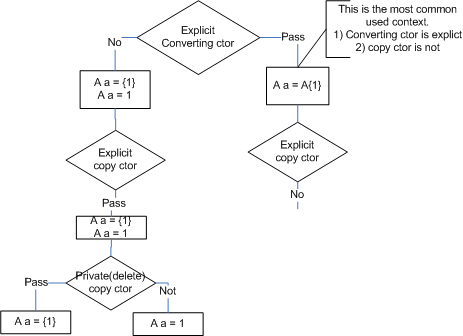
\includegraphics[width=0.8\linewidth]{pics/copy_init.png}
	%\caption{}
	%\label{Explicit and init }
%\end{figure}

%\begin{tabular}{|p{0.27\textwidth}|p{0.6\textwidth}|}
	%\tophline
	%Expression & meaning \\
	%\tophline
	%A a = (i), A a=\{i\} & explicit converting constructor will not work \\
	%\tophline
	%A a = A(i), A a = A\{i\} & explicit copy constructor will not work 
	%\bottomhline
%\end{tabular}


%%\item Last summary about previous three sections.
%%\begin{figure}[h]
%%	\centering
%%	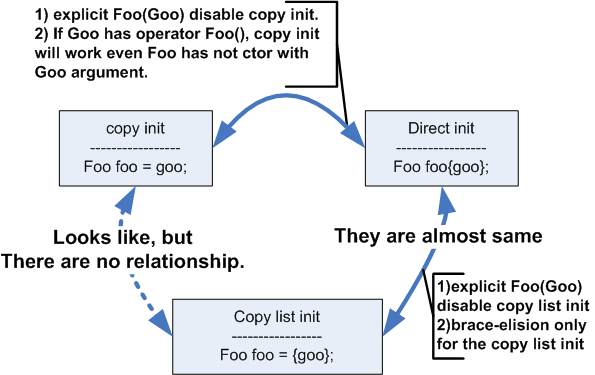
\includegraphics[width=0.9\linewidth]{pics/copy_list.png}
%%	\caption{difference between direct, copy and list-copy init}
%%	\label{fig:copylist}
%%\end{figure}

%\end{itemize}

\section{List initialization}

\subsection{Basic syntax}
\begin{itemize}
		
	\item List initialization is just a new syntactic form. \textbf{You can use list initialization syntax on three initializations forms.} Please note here, value list initialization can be thought as value initialization too.  
	\begin{enumerate}
		\item Value list initialization. It can avoid vexing parsing problem
\begin{lstlisting}[numbers=none]
T object{};
T{};
new T{}
Class { T member{}; };
: member{}  // Class member initializer lists
\end{lstlisting}

		\item Direct list initialization.
\begin{lstlisting}[numbers=none]
T object{arg, ...};
T {arg, ...};
new T{arg, ...}

Class {  // Class member initializer
	T member{arg, ...}; 
};
		
: member{arg, ...} // Class member initializer lists
\end{lstlisting}

		\item Copy list initialization. It has a equal sign in it or function parameter and return.
\begin{lstlisting}
T object = {arg, ...};
object = {arg, ...};
Class { T member = {arg, ...}; }; //Class member default initializer
function({arg, ...}); //Initializes temporary for the function arg
return {arg, ...};  //Initializes temporary for return value
\end{lstlisting}
	\end{enumerate}
		
\item Detail syntax analysis and comparison.
\begin{lstlisting}[frame=single, language=c++,mathescape=true]
widget w;               // (a)
widget w();             // (b)
widget w{};             // (c)
	
widget w(x);            // (d)
widget w{x};            // (e)
	
widget w = x;           // (f)
widget w = {x};         // (g)
	
auto w = x;             // (h)
auto w = widget{x};     // (i)
\end{lstlisting}
	
	\begin{enumerate}
		\item (a) is just default initilaiztion with default constructor.
		
		\item \textbf{(b) is function declaration.} That is why we prefer use brace initialization (c), it will avoid this vexing problem.
		
		\item For (d) and (e), These are both direct initialization. The variable w is initialized "directly" from the value of x by calling \texttt{widget::widget(x)}. If x is also of type widget, this invokes the copy constructor. Otherwise, it invokes a converting constructor.
		
		\item (e) is better than (d) to avoid narrowing, for example: \texttt{int a(1.2)} pass, but \texttt{int a{1.2}} fail.
		
		\item For (e), it prefer constructor that takes an \texttt{initializer\_list.} We will introduce more in \texttt{initializer\_list.} section.
		
		\item For (f), when \texttt{x} is type of widget, just like (d), but can't work when copy constructor is explicit(copy constructor never be explicit). When \texttt{x} is not type of widget, it will convert \texttt{x} to a temporary If \texttt{x} is of some other type, \textbf{conceptually} the compiler first implicitly converts x to a temporary widget object, then move-constructs w from that temporary rvalue, using copy construction as "the slow way to move" as a backup if no better move constructor is available. Assuming that an implicit conversion is available, (f) means the same as widget w( widget(x) );. Note that I said "conceptually" a few times above. That's because practically compilers are allowed to, and routinely do, optimize away the temporary and, if an implicit conversion is available, convert (f) to (d), thus optimizing away the extra move operation. However, even when the compiler does this, the widget copy constructor must still be accessible, even if is not called, the copy constructor's side effects may or may not happen.

		\item \textbf{For (g), This is called “copy list initialization.” It means the same as \texttt{widget w\{x\}};} except that explicit constructors cannot be used. It’s guaranteed that only a single constructor is called,(only converting constructor is called, no copy constructor).
		
		\item (h) just like type-of-x w(x), is same with (d), only single copy constructor is called
		
		\item (i) is the most consistent spelling when you do want to commit to a specific type and explicitly request a conversion if needed, and once again the \{ \} syntax happily avoids lossy narrowing conversions. In practice on most compilers, only a single constructor is called-similarly to what we saw with (f) and (g).
		
		\item Some initialization examples based on previous introductions.
		
\begin{lstlisting}[frame=single, language=c++,mathescape=true]
class Test{
public:
	int i;
	Test(int a = 0):i(a){}
	Test(const Test &T){ cout<<"copy constructor";} 
};
		
Test too = 2;  //test for (f) 
Test too = {2} // test for (g)
		
Test too;  
auto w = too //test for (h)
auto w = Test{2} //test for (i), no semantic difference with Test w{2};
\end{lstlisting}
\begin{description}
	\item[Line 8 and 9:] Both (f) and (g) work and no call copy constructor (no output:"copy ctor"); If converting ctor has explicit both fail,but \texttt{Test too\{2\}} succeed; if copy constructor is private, (f) fail, but (g) is still OK. Because \texttt{A a = \{b\};} is just like \texttt{A a(b);}

	
	\item[Line 13:] you can use \texttt{auto w = Test(2)}, it just call constructor, and \texttt{w} is not const reference. List initilization \{\} is better, it more generic and avoid narrow \texttt{auto w = Test\{1.2\}} fail, \texttt{auto w=Test(1.2)} ok. Even converting constructor is explicit, it can work too. No copy constructor is called at all.
\end{description}

	\end{enumerate}

\end{itemize}

\subsection{Traditional copy initialization and list copy initialization}

\begin{itemize}

	\item The basic syntax examples of list copy initialization. Does the equal sign make a difference in brace initialization? eg. '\texttt{T a = \{\}}' vs '\texttt{T a\{\}}' The only significant difference I know is in the treatment of explicit constructors:
	
\begin{lstlisting}
struct foo{
		explicit foo(int);
};
foo f0 {42};    // OK
foo f1 = {42};  // list initiliazation, fail here due to explicit
\end{lstlisting}

	\item Another important difference is a little subtle, can be demonstrated by below code:
	\begin{enumerate}
		\item traditional copy initialization uses notion of user-defined conversion sequences (and, particularly, requires availability of copy constructor, as was mentioned)
		
		\item \texttt{T a = \{\}} is like \texttt{T a\{\}}. So list copy initialization just performs overload resolution among applicable constructors, i.e. brace initialization can't use operators of conversion to class type
	\end{enumerate}
\begin{lstlisting}
struct Intermediate {};
struct S{
	operator Intermediate() { return {}; }
};
struct S1{
	S1(Intermediate) {}
};
	
S s;
Intermediate im1 = s; // OK
Intermediate im2 = {s}; // ill-formed
S1 s11 = s; // ill-formed
S1 s12 = {s}; // OK
\end{lstlisting}
	
	\begin{description}
		\item[Line 10:] copy initialization uses notion of user-defined conversion sequences (and, particularly, requires availability of copy constructor, as was mentioned)
		
		\item[Line 11:] list copy initialization just performs overload resolution among applicable constructors, i.e. brace initialization can't use operators of conversion to class type. Intermediate has not constructor with S as argument.
		
		\item[Line 12:] copy initialization can just set up one implicit conversion sequence. In this case 1) S change to Intermediate by operator, 2) from Intermediate to S1 by constructor.  You can see there are two implicit conversion.
		
		\item[Line 13:] list copy initialization use constructors, and it will do any implicit conversion it needs to match up argument types. In this case 1) S change to Intermediate by operator, 2) call S1's constructor and pass this temporary Intermediate. That is why it fail here.		
	\end{description}
	
	\item Copy list initialization also supports multiple arguments.
\begin{lstlisting}[frame=single, language=c++]
class A{
public:
	int i;
	explicit A(int a = 0):i(a){cout<<"one";}
	A(int a , int b ):i(a){cout<<"two";}
	A(const A &T){ cout<<"copy constructor";} 
};
		
A too = (1,2); 
A too = {1,2}; //work, call two parameter constructor. 
A fun(A);
fun({1,2}) {return{3,4};}
\end{lstlisting}
	\begin{description}
		\item[Line 9:] fail, it (1,2) became 2, then call single constructor() and comma is operator, it's different with \{\}.
		
		\item[Line 12:] Usually, we don't declare two parameter constructor as explicit. So we can also pass fun argument and return by using a copy list initialization form. You can see the expression is simple and it will call constructor directly. 
	\end{description}
	
	
	\item \textbf{Summary:}
	\begin{enumerate}
		\item Copy list initialization just performs overload resolution among applicable constructors
		
		\item Copy list initialization with multiple arguments constructor make function call and return easier, illustrated by the previous source code.
	\end{enumerate}
	
\begin{figure}[h]
    \centering
    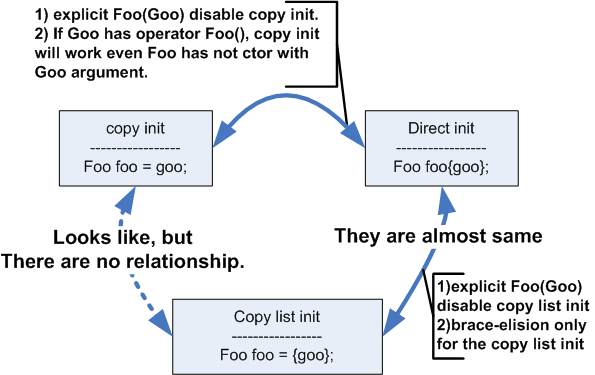
\includegraphics[width=0.45\linewidth]{pics/copy_list.png}
    \caption{difference between direct, copy and list-copy initialization.}
    \label{fig:copylist}
\end{figure}
	\item A good article is "Any difference between copy-list-initialization and traditional copy-initialization?"
	
	
\end{itemize}


\subsection{List initilization advantages}
			 

\subsubsection{Basic usage}
\begin{itemize}
	
	 \item \textbf{Empty brace is value init.} Value initialization of types usually means initialization to binary zeros.
\begin{lstlisting}[numbers = none]
int i{};     //i becomes 0, can't use () here         
double d{}; //  d becomes 0.0, can't use () here        
int *p{};   //initialized to nullptr
char s[12]{}; // all 12 characters are initialized to '\0'
char *p=new char [5]{};  //all five chars are initialized to '\0'		
std::string s{}; // s becomes "" can't use () here  
std::vector<float> v{}; //v becomes an empty vector
\end{lstlisting}

    \item List initialization can avoid narrowing problem.
\begin{lstlisting}[numbers=none]
double val = 7.4;
int i {val}; //error, possible truncation.
\end{lstlisting}

    \item Easy to create anonymous variable. In C++, anonymous variables are primarily used either to pass or return values without having to create lots of temporary variables to do so. anonymous objects are treated as rvalues (not lvalues, which have an address). This means anonymous objects can only be passed or returned by value or const reference. Otherwise, a named variable must be used instead.

\begin{lstlisting}[frame=single, language=c++]
Cents add(const Cents &c1, const Cents &c2){
	return Cents{c1.getCents() + c2.getCents()};
	// return anonymous Cents value
}

cout <<add(Cents{6}, Cents{8}).getCents();
\end{lstlisting}

    \item Omit type when you pass or return from function by using copy list initialization. it's future proof. If you later rename the class, the brace one will continue to work as is, while the parenthesis one will require a name change.

\begin{lstlisting}
MyClass2 fun (MyClass2 m) 
fun(MyClass2(2011,3.14)) //before c++ 11, fun ( (2011,3.14) ) doesn't work

fun ( {2011,3.14} ){
	return {2011,3.14};  //there is ; in the end
}

MyClass2 mc2;
mc2 = {2011,3.14}  // or MyClass2(2011, 3.14)
\end{lstlisting}

    \item Brace initialization support for more types. Next few example will demonstrate how to initialize aggregate, class member and STL container. This feature makes it easier to write more generic template function. 

\begin{lstlisting}[frame=single, language=c++,mathescape=true]
// C++98 
double *pd= new double [3]; // can't initilize them
rectangle w( origin(), extents() ); //vexing problem
vector<int>     v;  //need for loop to initilize it
for( int i = 1; i <= 4; ++i ) v.push_back(i);

// C++11 (note: "=" is mostly optional)
double *pd= new double [3] {0.5, 1.2, 12.99};
rectangle     w   = { origin(), extents() }; 
vector<int>   v   = { 1, 2, 3, 4 };
std::map<std::string,int> myMap{{"Scott",1976}, {"Dijkstra",1972}};
\end{lstlisting}

\item A non-static data member initializer (NSDMI) must use a brace-or-equal-initializer.
\begin{lstlisting}[frame=single, language=c++, mathescape=true]
class Foo{
public:
	Foo(): myData{1,2,3,4,5}{} // can initialize directly.
private:
	int myData[5];
	int equals = 42;                      //OK
	std::unique_ptr<Foo> braces{new Foo}; //OK
	std::vector<int> bad(6);  // 6 elements, all value are 0.
	std::vector<int> good{6}; // 1 element, value is 6. 
};
  	\end{lstlisting}
	
\item List initialization can be used on many different kind of type. This flexible ability isn't just an aesthetic issue. Consider writing generic template code that should be able to initialize any type. Using perfect forwarding as an example:

\begin{lstlisting}[frame=single, language=c++,mathescape=true]
template<typename T, typename ...Args>
void forwarder( Args&&... args ) {
T local = { std::forward<Args>(args)... };
// ...
}
//All below statement can work because we have list initialization.
forwarder<int>            ( 42 );                  
forwarder<rectangle>      ( origin(), extents() ); 
forwarder<complex<double>>( 2.71828, 3.14159 );    
forwarder<mystruct>       ( 1, 2 );                
forwarder<int[]>          ( 1, 2, 3, 4 );          
forwarder<vector<int>>    ( 1, 2, 3, 4 );          
\end{lstlisting}

	\item A good reference article is GotW \#1 Solution: Variable Initialization or Is It? Another good one is Overview of C++ Variable Initialization. address is \\ \verb=https://greek0.net/cpp/initialization.html=
	
	\item \textbf{Summary of brace initialization advantage:}
\begin{enumerate}
	\item Avoid narrowing problem.
	\item Support value initialization.
	\item Avoid vexing problem. (Introduced in the next section.)
	\item Input and return temporary variable easier. Using \{\} directly without type name. 
	\item More aggregated initialization.
	\item More uniform syntax, for aggregated, class member and STL container. 
\end{enumerate}
\end{itemize}


\subsubsection{Vexing parsing}
\begin{enumerate}
	\item The basic reason behind of vexing parsing come from C++ standard: \textbf{"If it can be a function declaration, it is".}
	
	\item Use parentheses to group when you declare a variable. \textbf{When you declare something, It's legal to use parentheses to group variable name.} Sometimes, you have to use parentheses, such as declare a function pointer. 
\begin{lstlisting}[frame=single, language=c++, mathescape=true]
int f(int);   //a function return a int
int *f(int);  //a function return pointer
int (*f)(int); //a function pointer;  
\end{lstlisting}
	
	\item It also means that you can have below C++ statements. The whole idea is just like to make (2+3)*4 work, you have to make parentheses applicable, so although unnecessary, (2)+(3) must be a legal statement.
\begin{lstlisting}[frame=single, language=c++, mathescape=true]
int x;
int (x); //same as above
int f(int x);
int f(int (x)); //same as above
\end{lstlisting}
	
	\item For function declaration, you can omit the parameter name.  
\begin{lstlisting}[frame=single, language=c++, mathescape=true]
int f(int x);
int f(int (x));
int f(int); //three statements are same. 
\end{lstlisting}
	
	\item For object, thing becomes interesting.
\begin{lstlisting}[frame=single, language=c++, mathescape=true]
int (x); // just like int x;

class A{
	A(int a);
...}
	
int a = 10; 
A(a);
const A& ar = A(a); //this is OK

(A(a)); //If you really want a temporary A object, use another parentheses. 
\end{lstlisting}
\begin{description}
	\item[Line 8:] You want to create a temporary obj, but compile think it as A a; It trigger compiler error, redefine \texttt{a}, because \texttt{a} has been defined in line 7.
\end{description}
	
	\item Below are all interpreted as function declaration. 
\begin{lstlisting}[frame=single, language=c++, mathescape=true]
int f(double (*pf)()); //standard way
int f(double pf()); //You can omit parentheses, just like int x and int (x);
int f(double ()); //for function f, you can omit variable name.
\end{lstlisting}
\begin{description}
    \item[Line 2] Function arguments are adjusted to be a pointer to function arguments. That is only applicable in function parameter context. 
\end{description}

	\item With all previous introduction, we see confused phenomena when we want to use or define a temporary C++ object. 
\begin{lstlisting}[frame=single, language=c++]
class Foo{
	......
};
	
Foo x(); //this is function declaration, you should use Foo x; or Foo x{};
	
Foo x(Foo());  // a function
Foo x(Foo(i)); //a function, Foo(i) equal Foo i; because () can be omitted by a compiler.
//vs.
Foo y{Foo{}};  // a variable, build with a temporary Foo
\end{lstlisting}
\begin{description}
	\item[Line 7:] declare a function \texttt{x}, receive a function pointer \texttt{Foo ()}, return Foo. Here, We omit the function parameter name, That is to say,  \texttt{Foo (*para) ()}  equals \texttt{Foo  ()} in this context.
	
	\item[Source code:]  Why \texttt{Foo(i)} equal \texttt{Foo i}; but \texttt{Foo()} equal a function pointer? If \texttt{Foo(int)}, then it will be a function pointer.  function declaration need type name, not a variable name, such as \texttt{i}.	
\end{description}

	\item Before C++11, you need add another pair parentheses to change it from declaration to expression. After C++11, you can use braces.
\begin{lstlisting}[frame=single, language=c++, mathescape=true]
Foo a{Foo{x}}; 
Foo a{Foo{}};
\end{lstlisting} 

	
	\item The most complex problem. A range container constructor. 
\begin{lstlisting}[frame=single, language=c++, mathescape=true]
list<int> data(istream_iterator<int>(dataFile), istream_iterator<int>()); //error
list<int> data(istream_iterator<int>{dataFile}, istream_iterator<int>{}));//OK
\end{lstlisting}
\begin{description}
	\item[Line 1:] \texttt{data} is function. First parameter is \texttt{dataFile}, type \texttt{istream\_iterator<int>}, second parameter is function pointer. The First, you can add () around parameter name;  the second, you can omit parameter name.
\end{description}
		
	\item \textbf{Summary:} Vexing problem happens when 1) using (), 2) use unname temporary variable to initialize another variable. We can use brace initialization to fix this problem. A good refernce is \verb|https://timesong-cpp.github.io/cppwp/n4140/stmt.ambig| or google search 
	"everything that can be a declaration is a declaration" 
	
\end{enumerate}



\section{Initilizer\_list and auto}
\subsection{initilizer\_list}
\begin{itemize}
	\item The whole problem comes from initializing method of array in C language. But this way can't be use in C++ container object. In the generic programming, we need to use the "uniform initializer". It  makes the \texttt{vt} and array use the same syntactic usage. In order to make it possible, C++11 introduces \texttt{std::initializer\_list} template. It's the proxy class. We need vector to have a constructor with \texttt{initializer\_list} parameter.
\begin{lstlisting}[frame=single, language=c++,mathescape=true]
int array[] = {1,2,3,4,5}  //OK 
vector<int> vt = {1,2,3,4,5} //doesn't work before C++11 

vector( std::initializer_list<T> init)
vector<int> vt = {1,2,3,4,5} //Work, call previous constructor
\end{lstlisting}
		
	\item In STL library, list, vector, map support \texttt{initializer\_list} constructor. You also can use it in your own class, function or for range.
\begin{lstlisting}[frame=single, language=c++,mathescape=true]
void f(const initializer_list<string> &slst){
	....
}
f({ "Good", "morning", "!" });
	
// A braced-init-list can be implicitly converted to a return type.
vector<int> test_function() { return {1, 2, 3}; }
	
// Iterate over a braced-init-list.
for (int i : {-1, -2, -3}) {}
	
// Call a function using a braced-init-list.
void TestFunction2(vector<int> v) {}
TestFunction2({1, 2, 3}); 
\end{lstlisting}

	\item  \textbf{You should not only judge \texttt{initializer\_list} by braces}. There are four points:
	\begin{enumerate}
		\item The class should have a \texttt{initializer\_list} constructor 
		\item It uses braces to initialize.
		\item The number of parameter inside braces is flexible but the type should be the same.
	\end{enumerate}

\begin{lstlisting}[frame=single, language=c++,mathescape=true]
vector( std::initializer_list<T> init)
vector<int> vt = {1,2,3,4,5} //call the constructor in line 1.
	
struct A{
	int i;
	int j;
};	
A a = {1, 2} // list initilization, not initializer_list
\end{lstlisting}
	
	\item Mostly, list initilization and \texttt{initializer\_list} can be used together. For example if you want to initialize a map you can use an \texttt{initializer\_list} of list initialization of the key value pairs: Here, the type of the pairs is clear and the compiler will deduce, that '{"Alex", 522}' in fact means \texttt{std::pair<std::string const, int>\{"Alex", 522\}}.
	
\begin{lstlisting}[frame=single, language=c++,mathescape=true]
std::map<std::string, int> scores{ 
	{"Alex", 522}, {"Pumu", 423}, {"Kitten", 956} 
};
\end{lstlisting}

	\item An empty pair of braces can be value initialization or An empty \texttt{std::initializaer\_list}. You should know how to distinguish them.  Empty braces mean no arguments, that is to say you get default construction, not an empty \texttt{std::initializer\_list}:
\begin{lstlisting}[frame=single, language=c++,mathescape=true]
class Widget{
public:
	int i;
	Widget(){cout<<"default";}
	Widget(initializer_list<int>){cout<<"init";}
};
	
Widget w1; // calls default constructor.
Widget w2{};  //calls default constructor too.
Widget w3(); // most vexing parse! declares a function!
	
Widget w4({});//std::initializer_list constructor with empty list 
Widget w5{{}}; //Same
\end{lstlisting}
	
	\item When non-empty list initilization is used and there are overload \texttt{initializer\_list}.
	\textbf{it always match initializer\_list}.
\begin{lstlisting}[frame=single, language=c++,mathescape=true]
class Widget {
public:
	Widget(int i, bool b); // as before
	Widget(int i, double d); // as before
	Widget(std::initializer_list<long double> il);
};
	
Widget w1(10, true); //  calls first constructor
Widget w1{10, true}; // std::initializer_list constructor
// (10 and true convert to long double)

Widget w2(10, 5.0); //  calls second constructor
Widget w2{10, 5.0}; // std::initializer_list constructor
// (10 and 5.0 convert to long double)
\end{lstlisting}
\begin{description}
    \item[Line8-9] Compilers' determination to match braced initializers with constructors taking \\ \texttt{std::initializer\_lists} is so strong, it prevails even if the best-match \\ \texttt{std::initializer\_list} constructor can't be called.
\end{description}
	
	\item An example from vector, () and list initilization are different in meaning. Based on vector example, choosing between parentheses and braces for object creation inside templates can be challenging. (it has different semantic meaning.)
	
\begin{lstlisting}[frame=single, language=c++,mathescape=true]
std::vector<int> v1(10, 20); 
std::vector<int> v2{10, 20}; 
\end{lstlisting}
\begin{description}
	\item[Line 1:] use non-std::initializer\_list constrouctor: create 10-element vector, all elements 20.
	\item[Line 2:] use initializer\_list constructor, create 2-element vector, element are 10 and 20
\end{description}
	
	
	
	
\end{itemize}

\subsection{Auto initilization(Almost Always Auto)}

\subsubsection{Basic usage}
\begin{itemize}
	\item \textbf{Three main usage of \texttt{auto}}:
	\begin{enumerate}
		\item Initialization. For example, you can assign lambda to an auto type.
		\item auto parameter in lambda.
		\item auto return type.  with help of auto parameter and auto type, you can build \textbf{generic lambda}. in this field, you need to know when to use \texttt{decltype(auto)}.
	\end{enumerate}

	\item The basic usage of auto initialization is: auto sets the type of a declared variable from its initializing expression while compiling. When you use an expression to initialize a variable, prefer to use \texttt{auto}.
\begin{lstlisting}[numbers=none]
auto a = expr
auto a = T{expr} //when you want to commit to type

auto s = "Hello";  //s is const char* just like const char* s = "Hello";
auto str = string{"Hello"} // this time is string
auto p = &x  //prefer to use auto* p, because it stresses the intent
auto v = {1, 2, 3}    // std::initializer_list
auto vect = vector<int>{1,2,3} // this time is vector.

auto p = new vector<pair<int, string> >; //don't need pointer type
std::vector<std::pair<int, std::string>> array;
auto it = array.begin();    //don't need containter iterator type
//unique_ptr<widget> w = make_unique<widget>();
auto w = make_unique<widget>(); //template class or function.

auto l = [](){..}; //lambda
double fm(double, int);
auto pf = fm  //pf is function pointer.        
\end{lstlisting}
	
	\item About the auto \texttt{type} deduction, please refer to the next chapter Generic programming type inference section. The basic idea is quite simple: \textbf{take exactly the type on the right-hand side, but strip off top-level const/volatile and reference \&/\&\&.} If you want your auto declaration to be \texttt{const}, or if you want your \texttt{auto} declaration to be a reference, you have to add them explicitly.
	
\begin{lstlisting}[frame=single, language=c++]
const auto iter = modmap.find(123); //specify const
auto& mod = vec[17];      //specify &
for (const auto& element : myarray) {
	//do stuff that reads from element
}
\end{lstlisting}
	
	\item auto can be used in template function return type
\begin{lstlisting}
template <typename F, typename T>
auto apply(F&& f, T value){
	return f(value);
}
\end{lstlisting}

	\item Four advantages:
	\begin{enumerate}
		\item avoidance of uninitialized variables.
\begin{lstlisting}[numbers=none]
auto x2; // error! initializer required
auto x3 = 0; // fine, x's value is well-defined
\end{lstlisting}

		\item avoidance of verbose variable declarations.
\begin{lstlisting}[frame=single, language=c++]
template<typename It>
void dwim(It b, It e) {
//typename std::iterator_traits<It>::value_type currValue = *b;
auto currValue = *b; //using auto is simple
	
auto ii = find_if(people.begin(), people.end(), match_name );               
if (ii != people.end()){...}
\end{lstlisting}

		\item Avoid what I call problems related to "type shortcuts." \textbf{It's very importance here, it guarantee correct and performance}
\begin{lstlisting}[frame=single, language=c++]
std::vector<int> v;
		...
int sz = v.size();
auto sz = v.size();
		
std::unordered_map<std::string, int> m;
for (const std::pair<std::string, int>& p : m){
	... // do something with p
}

for (const auto& p : m){
	... // as before
}
\end{lstlisting}
\begin{description}
	\item[Line 4:] \texttt{v.size()} return \texttt{size\_t}.
	\item[Line 11:] pair type is \texttt{<const std::string, int>}. When you use auto, you don't have this error
\end{description}
	\item Good maintenance.
\begin{lstlisting}[frame=single, language=c++, mathescape=true]
struct record {
	std::string name;
	int id;
	//GUID id; 
};

//int find_id(const std::vector<record> &people...
auto find_id(const std::vector<record> &people, 
                                  const std::string &name)
\end{lstlisting}
\begin{description}
	\item[Source code] First, change id type in line 3 to line 4, if we use auto in line 8, we dont' need to change at all. But if we use int, then we need to change from int to GUID too.
\end{description}

	\end{enumerate}
\end{itemize}
	
\subsubsection{pitfall of auto}
	There are two points need to be noticed. The first one is using \texttt{auto} with \texttt{vector<bool>}, The second is combining \texttt{auto} with list initialization.
	\begin{enumerate}
		\item "invisible" proxy classes. An invisible proxy class example is \texttt{vector<bool> []} operator. \texttt{vector<bool>::operator[]} neither yields a bool nor a reference to a bool. It just returns a little proxy object that acts like a reference. This is because there are no references to single bits and vector<bool> actually stores the bools in a compressed way. So by using auto you just created a copy of that reference-like object. The problem is that C++ does not know that this object acts as a reference. You have to force the "decay to a value" here by replacing auto with T
\begin{lstlisting}
template <typename T>
void Test(const T& oldValue, const T& newValue, const char* message){
	vector<T> v;
	v.push_back(oldValue);
	cout << " before:  v[0] = " << v[0] << '\n';
	auto x = v[0]; // Should be a deep-copy
	x = newValue;
	cout << " after:   v[0] = " << v[0] << '\n';
}

int main(){
	Test<int>(10, 20, "Testing vector<int>");
	Test<bool>(true, false, "Testing vector<bool>");
}
\end{lstlisting}
\begin{description}
	\item[Line 6:] When we use auto here, it get proxy classes, not bool value. so when we modify x, it will modify x[0] directly.
	
	\item[Source code:] before:  v[0] = 1; after:   v[0] = 0;Because it returns reference,  so v[0] has been modified. If you don't understand why, no worry. I will introduce \texttt{std::ref} in the Concurrent chapter, you can go there to look the introduction of \texttt{std::ref}. Both "proxy" class and \texttt{std::ref} share the same idea.
\end{description}

\begin{center}
	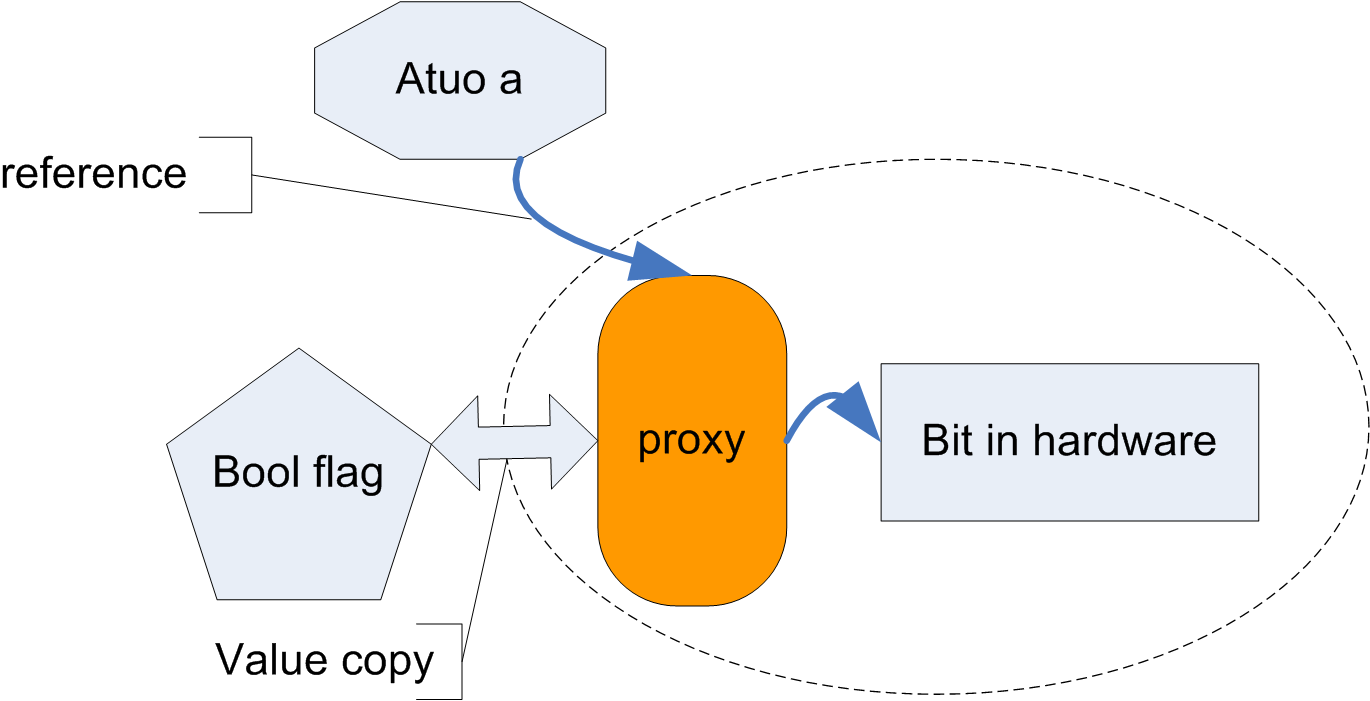
\includegraphics[width=0.45\linewidth]{pics/auto2.png}
\end{center}

		\item initilization brace return \texttt{std::initializer\_list<int>}. Prior to C++17 the type for all the following objects (a, b, c and d) is deduced to \texttt{std::initializer\_list<int>}. There is no difference between the direct-list-initialization and the copy-list-initialization on the result of the type deduction. 
		
\begin{lstlisting}[numbers=none]
auto a = {42};   // std::initializer_list<int>
auto b {42};     // std::initializer_list<int>
auto c = {1, 2}; // std::initializer_list<int>
auto d {1, 2};   // std::initializer_list<int>
\end{lstlisting}
		\texttt{auto b\{42\}} produces \texttt{std::initializer\_list<int>}, that is not nature. So C++17 introduced the following rules: 

    \begin{enumerate}
		
		\item  For copy list initialization auto deduction will deduce a \texttt{std::initializer\_list<T>} if all elements in the list have the same type, or be ill-formed.
		
		\item for direct list initialization auto deduction will deduce a T if the list has a single element, or be ill-formed if there is more than one element.
\begin{lstlisting}[numbers=none]
auto a = {42};   // std::initializer_list<int>
auto b {42};     // int
auto c = {1, 2}; // std::initializer_list<int>
auto d {1, 2};   // error, too many 
\end{lstlisting}

	\end{enumerate}
\end{enumerate}


\section{Initialization summary}

\subsection{Key points of this chapter}
\begin{itemize}
	
	\item There are three levels. 
\begin{center}
	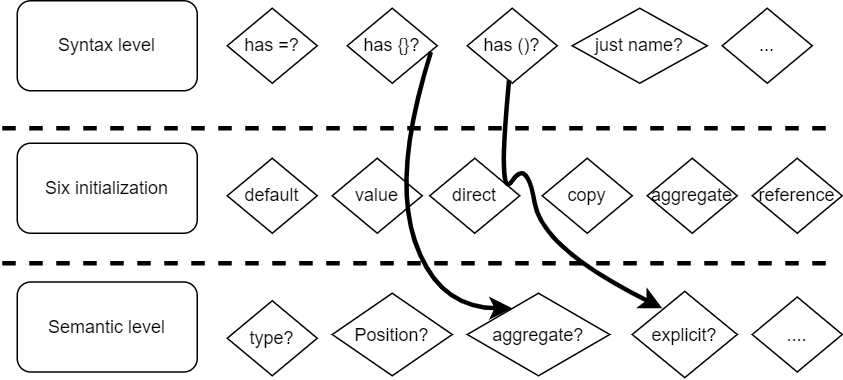
\includegraphics[width=0.80\linewidth]{pics/sum_init.png}
\end{center}	
	
	\item Brace initialization is called uniform init, you can see uniform is the biggest strengthen of this new feature. Most of the time, you result is obvious and simple. In order to achieve the uniform, \textbf{brace initialization must be able to deal with different kind of type, such as build in type, aggregate, class with different constructor etc.} it adds its complexity of analysis. We must read boring CPP document carefully to understand the different branch, different action when we use brace initialization on the different type. In another word, \textbf{List initialization is just in syntax level, for the detail initialization form, it depends on the specific data type.}  For example: If T is an aggregate type, \textbf{aggregate initialization} is performed. Otherwise, If the braced-init-list is empty and T is a class type with a default constructor, \textbf{value-initialization} is performed. In another word,\texttt{A a\{x,y\}} maybe a direct initilization, or an aggregate initilizaiton. \textbf{What kind of initilization is decided by the data type and syntax together.} That is very important point for you to understand better about initilization in C++.
	
\begin{lstlisting}
A a{}; //value initilization
A a{1};	
\end{lstlisting}	
	\begin{description}
		\item[Line 2:] Even you see brace here, but it can be direct initialization or aggregate initialization. \textbf{You can't judge initialization form only by existing of brace.} If A is aggregate type, then line 2 will proform aggregate initialization. If A has user-defined default constructor, then it will perform default initialization. 
	\end{description}
	
	
	\item Understanding some basic conceptions. such as aggregate type. copy-list-initilization, converting constructor. All the high level usages are based on these basic conceptions. Please see these conception in section "basic principles and terminology".
	
	\item \textbf{Familier with basic six initilization methods(forms).} You should know how to distinguish them. For example, when use = , it is called copy init. 
	
	\item \textbf{Six initilization methods and list initialization are irrelevant. list initialization syntax can be interpreted as aggregated init, value init, direct initialization or copy initialization and it brings its own advantage.} 
	
	\item List initialization is uniform initialization. How can it be uniform? Because for differnt T type, it carry out different actions, such as carry out value initialization or call converting constructor.

	\item Know the difference between value initialization and default initialization. 

	\item Know the difference between direct init, copy initialization and list copy initialization.  Direct initialization is the same as list copy init. they are different with copy init. Detail can be found in the previous two sections: "copy initialization and direct init". and "traditional copy initialization and list copy init"

\begin{lstlisting}
A a(1) or A a{1} //direct init
A a = 1;  //copy init
A a = {1}; //list copy init	
\end{lstlisting}	 
  
	\item Know when to use list initialization and it's advantage. A lot of people think that when we use brace init, it will prefer to use \texttt{list\_initilaizer}. Or when we use auto and brace init, it has strange behavior, (this will be introduce in auto initialization section). Based on previous point of view, I don't think that it's a problem, on the contrary, you can think that it's more "Uniform", That means that brace initialization can be used on more context. In fact, brace initialization is very good, just pay attention when the class has list\_initiaizer constructor, or when you use it with auto together.
	
	\item Know the basic usage of \texttt{initilizer\_list} and the difference between list init.
	
	\item know the auto usage and its pitfall.
 
	\item \textbf{Summary figure:}
	\begin{figure}[h]
		\centering
		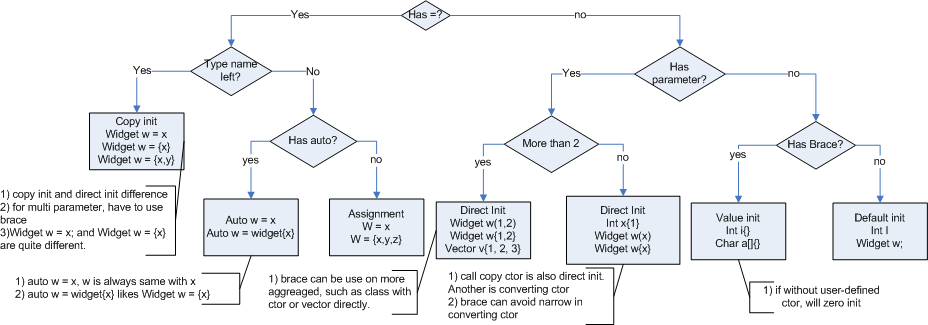
\includegraphics[width=0.95\linewidth]{pics/init.png}
		\caption{Overview of C++ init}
		\label{fig:command}
	\end{figure}
	
\end{itemize}

\subsection{How to analyze initialization expression}
\subsubsection{C++ standard}
\begin{itemize}
		
	\item I will analyze a real example, at the same time give C++ standard document. \textbf{The purpose of this example is how to analyze the complex initialization method in the future.}
\begin{lstlisting}
#include <iostream>
struct A {
	A(int i) : i(i) {}
	A() = default;
	int i;
};
		
int main() {
	A a{};
	cout<<a.i //output: 0, not random value
}
\end{lstlisting}
	
	\begin{description}
		\item[Line 9:]  The list initialization of \texttt{A}, Why it's list initilization? Because it use \{\}; *1 item satisfied, so perform value initilization. Please note here, *1~*5 item refer to "Extracts of C++ standard" below. Check *3 item, not satisfied, because we have default constructor. Then it meets all requirements in *4 item, so perform zeor-init.
	\end{description}
	
	
\begin{lstlisting}
#include <iostream>
struct A {
	int i;
	int j;
};
	
int main() {
	cout<<is_aggregate_v<A><<endl; //output: 1
    A a{1};
	cout<< a.i<<" "<<a.j<<endl; //output: 1 0
}
\end{lstlisting}
	
	\begin{enumerate}
		\item List initialization of A, Check *1 item but fail, \texttt{A} has no default constructor. \texttt{A} is aggregated type, according to *2 item, aggregate-initialization kick off.
		
		\item According to *5 item, \texttt{j} is initialized to 0		
	\end{enumerate}
	
	
	\item  Extracts parts from C++ standard: 
	
	\begin{quote}
		\verb|https://en.cppreference.com/w/cpp/language/list_initialization| \newline
		*1 (\textbf{For list initialization})If the braced-init-list is empty and T is a class type with a default constructor, value-initialization is performed. 
		\newline
		*2 Otherwise, if T is an aggregate type, aggregate initialization is performed.
		\newline
		
		\verb|https://en.cppreference.com/w/cpp/language/value_initialization|	\newline
		*3 if T is a class type with no default constructor or with a user-provided or deleted default constructor, the object is default-initialized; 
		\newline		
		*4 if T is a class type with a default constructor that is neither user-provided nor deleted (that is, it may be a class with an implicitly-defined or defaulted default constructor), the object is zero-initialized and then it is default-initialized if it has a non-trivial default constructor; \newline
		
	\verb|https://en.cppreference.com/w/cpp/language/aggregate_initialization|\newline
		*5 If the number of initializer clauses is less than the number of members and bases (since C++17) or initializer list is completely empty, the remaining members and bases (since C++17) are initialized by their default member initializers,
	\end{quote}
	
	\item \textbf{Summary:} Although C++ standard is not very easy to read, but it's very helpful. With the help of it, you can analyze the initialization syntax step by step. You can get the atomic and bottom level and know what initialization expression really does at last.
	
	\item A good article about this is "Initialization in C++ is Seriously Bonkers"
	
\end{itemize}

\subsubsection{Common used initilization syntax}
\begin{itemize}
	\item Given some basic definition below: 
\begin{lstlisting}[frame=single, language=c++]
class A{
	public:
	A(){};
	A(int k):m_a(k){};
	A(const A& rhs){m_a = rhs.m_a;};
	int m_a;
};

void fun(const A &a){}
int i = 3;	
\end{lstlisting}	
	
	\item Default constructor example:\\ 
	\begin{tabular}{|p{0.23\textwidth}|p{0.68\textwidth}|}
		\tophline
		Expression & meaning \\
		\tophline
		\texttt{A a, A a\{\}} & default constructor \\
		\tophline
		\texttt{A a()} & \textbf{declare function a,vexing problem} \\
		\tophline
		\texttt{A()} & A temporary A obj or declaration, detail is in vexing problem \\
		\tophline
		\texttt{B b(A())} & \textbf{declare function, vexing problem}, A() is function pointer \\
		\tophline
		\texttt{B b(A\{\})} & constructor a b with temp A. \\
		\tophline
		\texttt{fun(A()),fun(A\{\})} & pass an parameter to fun
		\bottomhline
	\end{tabular}

	\item single parameter constructor example: \\ 
	
	\begin{tabular}{|p{0.23\textwidth}|p{0.68\textwidth}|}
		\tophline
		Expression & meaning \\
		\tophline
		\texttt{A a(i), A a\{i\}} & parameterized constructor\\
		\tophline
		\texttt{A (i)} & \textbf{just like A i, you have define i, so compile error.} \\
		\tophline
		\texttt{A\{i\}} & A temporary A obj\\
		\tophline
		\texttt{B b(A(i))} & declare a function B b(A i); vexing problem \\
		\tophline
		\texttt{B b(A\{i\})} & build b with temp A\\
		\tophline
		\texttt{fun(A(i)),fun(A\{i\})} & work, fun(A i) will not a declaration, because there are no return value.\\
		\tophline
		\texttt{B b(A a(i))}  & compile error, because A a(i) is not expression. \\
		\tophline
		\texttt{fun(A a(i))} & same as above. \textbf{We need value for function parameter, not statement} 
		\bottomhline
	\end{tabular}
	
	\item Further explanation about previous table. Here we follow the basic C++ parsing rule: \textbf{If there is possible, it will use declaration first. }.
\begin{lstlisting}
int i = 5;
A(i); //redefine variable i, just like A i; compiler error
A a = A(i);
B b(A(i)); //function delcaration
B b(A a(i)); //compile fail
\end{lstlisting}	
	\begin{description}
		\item[Line 3:] \texttt{A(i)} will build temporary \texttt{A}, because there is assignment sign, so \texttt{A(i)} can't be declaration, otherwise it can't be suitable for the context.
		
		\item[Line 4:] interpret \texttt{A(i)} as declaration, and it suitable for the context.
		
		\item[Line 5:] For \texttt{B b(A a(i))}, compiler will first interpret it as function declaration first, but \texttt{A a(i)} is not declaration(it defines a variable a), ( \texttt{A(i)} and \texttt{A()} are both type). So it continue to interpret as B constructor, then it ask a value from expression. but \texttt{A a(i)} is not expression either, in the end, compiler is not happy. 
	\end{description}
			
\end{itemize}

\subsection{How to initialization by youself}

\begin{itemize}
	
		\item Basic rules:
	\begin{enumerate}
		\item If the (single) value you are initializing with is intended to be the exact value of the object, use copy (=) initialization (because then in case of error, you'll never accidentally invoke an explicit constructor, which generally interprets the provided value differently). In places where copy initialization is not available, see if brace initialization has the correct semantics, and if so, use that; otherwise use parenthesis initialization (if that is also not available, you're out of luck anyway).
		
		\item If the values you are initializing with are a list of values to be stored in the object (like the elements of a vector/array, or real/imaginary part of a complex number), use curly braces initialization if available. 
		
		\item If the values you are initializing with are not values to be stored, but describe the intended value/state of the object, use parentheses. In another word, if the constructor resembles a normal function call (it performs some more or less complex operations that are parameterized by the arguments) then using the normal function call syntax(parentheses). Examples are the size argument of a vector or the file name argument of an fstream. 
		
\begin{lstlisting}
vector<int> b{10,20};
vector<int> c(10,20);
vector<int> d{};
\end{lstlisting}
		\begin{description}
			\item[Line 2:] Curly braces -> fills the vector with the arguments
			\item[Line 3:] Parentheses -> uses arguments to parameterize some functionality, Like filling the vector with 10 integers.
			\item[Line 4:] Default initialization, use \{\}. For vector, maybe it's redundant, but it's good habit and keep your style consistency. For example, \texttt{int i}; and \texttt{int i\{\}}.
		\end{description}
	\end{enumerate}

	\item \textbf{Even you don't understand the whole chapter, just remember below steps when you are do initialization.}
	\begin{enumerate}
		\item When use same type to initialize, use copy initialization with equal sign.
\begin{lstlisting}
Foo f1 = f2; //best style
Foo f1(f2);  
Foo f1 = {f2}; 
\end{lstlisting}
\begin{description}
	\item[Line 2:] If f2 is not Foo type, then line 1 will fail with explicit single parameter constructor, but Line 2 will implicit convert and pass. That is not good.
	
	\item[Line 3:] It is just like line 2, it will fail with explicit single parameter constructor, but semantic is not as good as line 1.
\end{description}
		\item If right side is expression, new and function, Use \textbf{\texttt{auto var = expr;}}. 
		
		\item Otherwise, Use \textbf{list initialization if possible.} 
		
		\item When using list initialization, pay attention two traps for \texttt{std::initilizaer\_list.} 
		\begin{enumerate}
			\item If type has list initialization constructor, list initialization will use it first, and very strongly. vector is good example to explain this trap. At this time, please use parentheses instead.
\begin{lstlisting}
vector v1(1, 2);  //use parentheses describe vector 
vector v1{1, 2}; //use braces fill vector
\end{lstlisting}
			
			\item When we combine \texttt{auto} and list initialization together, it maybe deducts \\ \texttt{std::initilizaer\_list} type, maybe not.  You can see the section "pitfall of auto" 
		\end{enumerate}
	\end{enumerate}
	
\end{itemize}



\chapter{Memory}

\section{Memory functions in C}
\subsection{malloc}
\begin{itemize}
	\item That is a long story. In C language, if you forget a header file, what will happen? In one word, It will(c99) or will not produce(c89) warning, and compiler will assume a "implicit int" rule. That is to say, It presumes that the function without prototype (declaring in the header file) just return int type.
	
	\item Continue: if you have code below: you comment \texttt{stdlib.h}. Then compiler will assume that \texttt{malloc} return a \texttt{int}.  This code will run on 32 bit computer, because \texttt{int} and \texttt{int*} have same length. but on a 64 bit computer, \texttt{int*} is 64 bit and int is 32 bit.  so half data will be lost, and you code will crash. The worst is: if you add \texttt{(int*)} cast, it will suppress the warning message.(You kill the only clue, it's bad).
\begin{lstlisting}[frame=single, language=c++]
// include "stdlib.h"
int *sieve = (int *)malloc(sizeof(int)*length);
	
int *sieve = malloc(sizeof(int)*length);
\end{lstlisting}
\begin{description}
	\item[Line 2:] With explicit cast, it will NOT produce a (missing prototype)warning.
	\item[Line 4:] Without explicit cast, will produce a warning.
\end{description}

	\item continue: So don't recommend to use \texttt{(int*)} cast at all. Next question is that malloc actually return \texttt{void*}. Can \texttt{void*} automatically implicit be cast to \texttt{int*} or other pointer type in assignment? the answer is \textbf{YES}.
	
	\item  continue: In C language, we can use NULL to initiliaze pointer type.
\begin{lstlisting}[numbers=none]
#define NULL ( (void*) 0)
int *p = NULL;  //legal
FILE * f = NULL;  //legal
\end{lstlisting}
	
	\item continue: In C++, \texttt{int *p = (void *) 0} is not legal any more.(C++ is type safe language).  So in C++ NULL is literal 0. But It produce another ambiguity problem.  So In C++11, we define \texttt{nullptr} to resolve this problem.
\begin{lstlisting}[numbers=none]
cout<<is_integral<decltype(nullptr)>::value; //false
cout<<is_integral<decltype(NULL)>::value; //true

int *p = NULL; //illegal in C++
\end{lstlisting}

	
\begin{lstlisting}[numbers=none]
int *p = NULL; //illegal in C++
--------------------------------------
f(int i)
f(int * p);

f(NULL);  //will call f(int i).
f(nullptr) //will call f(int *p)
\end{lstlisting}
	
	\item \texttt{calloc()} zero-initializes the buffer, while \texttt{malloc()} leaves the memory uninitialized. Zeroing out the memory may take a little more time, so you probably want to use \texttt{malloc()} if that performance is an issue. If initializing the memory is more important, use \texttt{calloc()}. For example, \texttt{calloc()} might save you a call to \texttt{memset()}.
	
	\item When you use \texttt{memcpy}, the destination cannot overlap the source at all, but \texttt{memmove} can. This means that \texttt{memmove} might be very slightly slower than \texttt{memcpy}, as it cannot make the same assumptions. For example, \texttt{memcpy} might always copy addresses from low to high. If the destination overlaps after the source, this means some addresses will be overwritten before copied. \texttt{memmove} would detect this and copy in the other direction - from high to low - in this case. However, checking this and switching to another (possibly less efficient) algorithm takes time.
\end{itemize}

\subsection{realloc}
\begin{itemize}
	
	\item Reallocates the given area of memory. It must be previously allocated by \texttt{malloc()}, \texttt{calloc()} or \texttt{realloc()} and not yet freed with a call to free or \texttt{realloc}. Otherwise, the results are undefined. realloc may or may not change the original address. 

\begin{lstlisting}[]
str = (char *) malloc(15);
strcpy(str, "tutorialspoint");
printf("String = %s,  Address = %p\n", str, str);

/* Reallocating memory */
str = (char *) realloc(str, 25);
strcat(str, ".");
printf("String = %s,  Address = %p\n", str, str);
\end{lstlisting}
\begin{description}
	\item[Line 6:] Change 25 to 16, address of \texttt{str} doesn't change.
\end{description}

	
	
	\item Don't return value assign to input \texttt{ptr}, use another local pointer, such as \texttt{new\_ptr;}. Because if realloc fails, it will not overwrite original \texttt{ptr}.
\begin{lstlisting}[numbers=none]
void *new_ptr = realloc(ptr, new_size);
if (!new_ptr) {
	// deal with error;
}
ptr = new_ptr
\end{lstlisting}
\end{itemize}


\section{new operator}
\subsection{Basic}
\begin{itemize}
	\item There are four sub-topics about new operator:
	\begin{enumerate}
		\item new\_handler
		\item no throw, but return \texttt{nullptr}(since c++11)
		\item placement new (not allocate, just constructor)
		\item operator new (just allocate, no constructor)
	\end{enumerate}
	
	\item new operator(new expression) and operator new are two different thins. \textbf{new operator call operator new.} 
	
	\item there is three kind of operator new.
\begin{lstlisting}[frame=single, language=c++]
void* operator new (std::size_t size);
void* operator new (std::size_t size, const std::nothrow_t& nothrow_value) noexcept;
void* operator new (std::size_t size, void* ptr) noexcept;
\end{lstlisting}
	
\begin{lstlisting}[frame=single, language=c++]
std::set_new_handler(noMem);
MyClass * p1 = new MyClass;  

MyClass * p2 = new (std::nothrow) MyClass; 

new (p2) MyClass;  
MyClass * p3 = (MyClass*)::operator new (sizeof(MyClass));
\end{lstlisting}
\begin{description}
	\item[Line 2:] If fail, call noMem. If noMem is \texttt{nullptr}, throw \texttt{bad\_alloc} exception.
	\item[Line 4:] no throw, remember this constant \texttt{std::nothrow}.
	\item[Line 6:] placement new
	\item[Line 8:] operator new, allocates memory by calling: \texttt{operator new}. but does not call MyClass's constructor
\end{description}	

\item nothrow new just make sure that operator new inside will not throw exception, but return nullptr if allocation fails. but it will not assure that MyClass construtor will not throw exception. So it's not fullly mature design. \textbf{In other word, we don't recommend using this kind of nothrow new operator in the production code.}

\begin{lstlisting}[frame=single, language=c++]
MyClass * p2 = new (std::nothrow) MyClass; 
\end{lstlisting}


	\item \texttt{new operator} will call constructor function of a class, but \texttt{malloc} will not call constructor function.  \textbf{So in C++, you should use new operator instead of \texttt{malloc}.}
	
	\item For default new operator, you can use \texttt{set\_new\_handler} to adjust the behavior when you can't allocate enough memory. Detail can be found in the next section.
	
	
	\item If you use\texttt{ new int[100]}, don't forget \texttt{delete []};  \textbf{Any time you want to use new to allocate an array, ask yourself if you can replace it with vector or string.}
\end{itemize}

\subsection{Inside of new operator}
\begin{itemize}
    \item What happen when you call new operator? \textbf{new operator calling operator new, operator new calling new\_handler.} 
	
	\item Basic logic of new operator and delete operator. Below are C++ pseudo code.
\begin{lstlisting}[]
Point3d *origin = new Point3d;
	
if(origin = operator new(sizeof(Point3d))){
	try{
		origin = Point3d::Point3d(origin);
	}
	catch(...){
		operator delete(origin);
		throw
	}
}
\end{lstlisting}
\begin{description}
    \item[Line 3:] call operator new to allocate space in memory. (different with new operator), in this way, constructor will not be called.
    \item[Line 5:] call constructor of a class. (You can't call ctor explicit in this way, but compiler can.)
    \item[Line 8:] If constructor throw an exception, no memory leak by calling operator delete.
\end{description}
	
\begin{lstlisting}[]
delete origin;
	
if (origin != NULL) {
	origin->~Foo();
	operator delete(origin);
}
\end{lstlisting}
\begin{description}
    \item[Line 4:] So for a class, if you declare its destructor private or protected, You can't use "delete p".
\end{description}
	
\item Basic logic of operator new. This is throw version operator new, non-throw and placement operator new are alike. 
\begin{lstlisting}[frame=single, language=c++]
void * operator new(std::size_t size) throw(std::bad_alloc){
using namespace std; 
	if (size == 0) {   
		size = 1;             
	}                 
	void *last_alloc;
	while (true) {
		*last_alloc = malloc(size)
		if (last_alloc)
			return last_alloc;
		new_handler globalHandler = set_new_handler(0);
		set_new_handler(globalHandler);
		if (globalHandler) 
			(*globalHandler)();
		else 
			throw std::bad_alloc();
		}
}
	\end{lstlisting}
\begin{description}
	\item[Line 3:] handle 0-byte requests by treating them as 1-byte request. If size is 0, change it to 1. C++ standard requires it.
	
	\item[Line 11:] allocation was unsuccessful; find out what the current new-handling function and call it.

    \item[Source code:] Why we need to call \texttt{set\_new\_handler} twice, The first one get the current handler, and the second one changes it back. That is only way we can get the current handler. This idiom is also used in \texttt{set\_terminate} and \texttt{set\_unexpect}. Most of time, we use \texttt{malloc} and \texttt{free} to allocate and free physical memory. In C++11, introduce \texttt{get\_new\_handler()} function. We don't need to call \texttt{set\_new\_handler} twice. 
\end{description}

\item Basic logic of operator delete.
\begin{lstlisting}[numbers=none]
operator delete (void *ptr){
	if (ptr)
		free(ptr)
	}
\end{lstlisting}

\end{itemize}

\subsection{new\_handler}
\begin{itemize}	
	
	\item A real example of function pointer in C++ standard library is \texttt{set\_new\_handler}. It accepts a function pointer and return the same function pointer, so declaring such format is a little difficult.
\begin{lstlisting}[frame=single, language=c++]
void failNew(){
	cerr<<"Fail now"<<endl
	abort();
}
-----------------------------------------
extern void ( *set_new_handler ( void (*)() ) ) ();
			
set_new_handler(failNew);
\end{lstlisting}
		\begin{description}
			\item[Line 6:] This function declaration is very complex. 
		\end{description}
		
		\item A better method is to use typedef method.
		
\begin{lstlisting}[numbers = none]
typedef void(* FunPtr)();
FunPtr (*set_new_handler) (FunPtr);
set_new_handler(failNew);
\end{lstlisting}	
	
	\item At program startup, \texttt{new\_handler} is a null pointer. When allocation fail inside of operator new, operator new finds that \texttt{std::get\_new\_handler} returns a null pointer value, it will throw \texttt{std::bad\_alloc}.
	
	\item  As shown by the previous item, The \texttt{new\_handler} function is the function called by allocation functions whenever a memory allocation attempt fails. Its intended purpose is one of three things:
	
	\begin{enumerate}
		\item make more memory available. \textbf{resolve the problem by myself.}
		
		\item throw exception of type \texttt{std::bad\_alloc} or derived from \texttt{std::bad\_alloc}. \textbf{resolve the problem by a caller.}
		
		\item terminate the program. e.g. by calling \texttt{std::terminate}. \textbf{(No resolve)}
	\end{enumerate}
	
\begin{lstlisting}[frame=single, language=c++]
void noMemory(){
	closeIE;  //method1
	set_new_handler(nullptr);  //method2
	abort();  //method3
}
//in the beginning of main() function.
set_new_handler(noMemory)
\end{lstlisting}
\begin{description}
	\item[Line 2: ] method 1: release mem by close some current applications.
	\item[Line 3: ] method 2: throw \texttt{bad\_alloc} exception. If we set \texttt{new\_handler} \texttt{nullptr}, then operator new will throw \texttt{bad\_alloc} later.
	\item[Line 4: ] method 3: end application.
\end{description}
	

	\item If you want to have customized \texttt{new\_handler} for specific class, "effective C++ item 49" gives a good example. It use Mixin idiom. Detail can be found in generic programming section in this book.
\end{itemize}

\subsection{array new}
\begin{itemize}
	\item \textbf{Any time you want to use array new, think that if vector can do what you want? if answer is YES, don't use array new.} When you use array new to allocate an array, must use the array delete. If you don't use array delete, maybe you just delete the frist object in array. If you use array delete to single new, it's undefined. 
\begin{lstlisting}[frame=single, language=c++]
Foo pa* = new Foo[10];
delete [] pa;
\end{lstlisting}

\begin{description}
	\item[Line 2:] system will remember the size corresponding with pa,  with [], it will iterate with size.  When you forget [], it will just free the first object, cause memeory leak.
\end{description}

	\item Basic logic of array new. An basic implementation can be found in"Inside the C++ Object Model" 6.2 chapter
\begin{lstlisting}[numbers=none]
vec_new(int elem_count, int size, funptr constructor){
	total_size = size*elem_count;
	ptr_array = new char[total_size];
	regist pair of ptr_array elem_count to system
	while(elem<end of address){
		(*constructor)(elem) //call the ctor
		elem+=size;
	}
}
\end{lstlisting}
	
	\item When you use array new with inheritance. There is one important thing to notice. Don't use base pointer to point the array with derived class. 
\begin{lstlisting}[frame=single, language=c++]
base *bp = new derived[10]; //always use derived *dp = new derived[10]
bp[2] 
	
delete [] bp;
\end{lstlisting}
\begin{description}
	\item[Line 2:] dangerous, undefined. size is wrong: \texttt{bp+sizeof(base)*2}
	\item[Line 4:] dangerous, 1)size is wrong, 2)it will call \texttt{base::~base()} destructor. 
	
	\item[Source code:] Why it's dangerous? When you use delete [] bp, it will think that is a base array, and each element in it is just base object, so virtual function doesn't play a role here. Please refer the section "inheritance" in this book for more detail. \texttt{bp[2]} is not pointer, polymorphism only work when we use pointer or reference.
\end{description}

\end{itemize}

\subsection{Placement new}
\subsubsection{How to use placement new operator}
\begin{itemize}
	\item Construct an object in memory you've already got a pointer to, use placement new. If you use placement new to create an object in some memory, you should avoid using the delete operator on that memory.  Detail can be seen in the book "C++ primer"
\begin{lstlisting}[frame=single, language=c++]
Foo* p;
void* raw = operator new(sizeof(Foo)*100);
	
try {
	p = new(raw) Foo();  
	p1 = new(raw+sizeof(Foo) ) Foo();
}
catch (...) {
	// oops, constructor throw an exception
	operator delete(raw);
	throw;  // rethrow the constructor's exception
}

p->~Foo(); //call dtor directly,
p1->~Foo(); //call dtor directly,
operator delete(buffer);  //don't call delete [] raw or delete raw.
\end{lstlisting}
\begin{description}
	\item[Line 2:] Don't catch exceptions thrown by the allocator itself. Return a void type pointer. When you just want to allocate memory, operator new is better than \texttt{malloc}, because it offers you more options: you can use \texttt{set\_handler}, or you can choose if you want to throw exception.
		
	\item[Line 5:] Call the constructor with raw as this.
	\item[Line 14-15:] The is one chance you should call destructor directly. In fact, you usually don't call destructor directly in C++.
	 \item[Line 16:] When you use \texttt{operator new} to allocate memory, use \texttt{operator delete} to free it. 
\end{description}
	
	\item Another example to use placement new in stack array. Learn how to use placement new in stack and how to use \texttt{reinterpret\_cast}.
\begin{lstlisting}[numbers=none]
struct ComplexType {
	int a;
	ComplexType() : a(0) {}
	~ComplexType() {}
};
int main() {
	char* dynArray = new char[256];
	//Calls ComplexType's constructor to initialize memory as a ComplexType
	new((void*)dynArray) ComplexType();
	
	reinterpret_cast<ComplexType*>(dynArray)->~ComplexType();
	delete[] dynArray; //Clean up memory once we're done
	
	//Stack memory can also be used with placement new
	alignas(ComplexType) char localArray[256]; //alignas() available since C++11
	new((void*)localArray) ComplexType();
	
	//Only need to call the destructor for stack memory
	reinterpret_cast<ComplexType*>(localArray)->~ComplexType();
}
\end{lstlisting}

\end{itemize}

\subsubsection{placement operator new}

\begin{itemize}
	
	\item If operator new receive another parameter beside that \texttt{size\_t}, that is called placement new. The one with \texttt{pMemory} parameter is a special placement new operator. But you need to know, any another parameter beside the \texttt{size\_t} can be called as "placement operator new", we can call them as non-pMemory version.
\begin{lstlisting}[]
void* operator new (std::size_t size, void* pMemory) throw();
void* operator new (std::size_t size, ostream& logStream) throw();
\end{lstlisting}
	
	\item If you define your own placement operator new(non-pMemory version). You must provide your own placement operator delete. Because when the constructor throw exception, it will call the corresponding customized placement operator delete. Detail can be found in "effective C++ item 52"
\begin{lstlisting}[frame=single, language=c++]
void* operator new (std::size_t size, ostream& logStream) throw();
Widget* pw = new(std::cerr) Widget
	
void operator delete(void* pM, ostream& logStream). 
\end{lstlisting}
\begin{description}
	\item[Line 4:] When Widget constructor throw exception, it will call operator delete. if no such function, placement new does nothing and memory leak.
\end{description}

		\item But when no exception is thrown,  you still need to use "normal" delete to free the memory which allocated by placement operator new if you need to.(For memory pool application, maybe you don't need to do it, just call destructor.)

\begin{lstlisting}[frame=single, language=c++]
void* operator new (std::size_t size, ostream& logStream) throw();
{
	p1 = malloc(); // allocate extra memory for some house keeping work.
	return malloc();
}
Widget* pw = new(std::cerr) Widget
	
delete pw;
\end{lstlisting}		
\begin{description}
	\item[Line 8] Here, you have to use "normal" delete if you allocate memory in your own placement operator new, but "normal" delete will not take care of \texttt{p1}. Usually, you means that you should not allocate any resource in your own placement operator new.
\end{description}

		\item In C++, after you define a name in a scope (e.g., in a class scope), it will hide the same name in all enclosing scopes (e.g., in base classes or enclosing namespaces), and overloading never happens across scopes. And when said name is operator new, If you provide any class-specific placement new, provide all of the standard forms(plain, placement, and nothrow). Otherwise, it will placement new will hide plain new and nothrow new. Detail can be found in "effective C++ item 52".
\begin{lstlisting}[frame=single, language=c++, mathescape=true]
class C {
	static void* operator new(size_t, MemoryPool&);
	// hides three normal forms
};
void* operator new(std::size_t); // plain new
void* operator new(std::size_t, std::nothrow_t) throw(); //nothrow new
void* operator new(std::size_t, void*);	//placement new	
\end{lstlisting}


	\item A good article is "The many faces of operator new in C++", It give  detail information about operator new and how to rewrite it. You can google it.
\end{itemize}



\section{Customize operator new}
\begin{itemize}
	\item You can't change "new operator" behavior, but you can override global "operator new" and overload class its own "operator new". Pay attention its argument and return \texttt{void*}. Below code is just a simple demo, In the \texttt{new\_handler} section, you can see a better operator new demo with support of call your own \texttt{new\_handler}. You need to combine above code and code in \texttt{new\_handler} section together. 
	
\begin{lstlisting}[frame=single, language=c++, mathescape=true]
//global operator new
void* operator new(size_t size){
	cout<<"Yan's own operator new" ;
	void* mem = malloc(size);
	if(mem)
		return mem;
	else
		throw bad_alloc();
	
class Foo{ //class operator new
public:
	static void* operator new(size_t size);
		..
	}
	void* Foo::operator new(size_t size){
	cout<<"Foo's own operator new";
	....
}
	
int *p = new int[100]; //output Yan's own operator new
Foo* fp = new Foo();  //output Foo's own operator new
\end{lstlisting}
	
	\item When you should provide your own operator new?  You want to add log function; You want to add some cookie before and after allocated memory(Visual Studio use this way to detect overflow in debug mode). You want to have quicker speed(memory pool). You want to have better alignment and so on.. In summary, in below three contexts:
	\begin{enumerate}
		\item Performance: the default memory allocator is designed to be general purpose. Sometimes you have very specific objects you want to allocate, chapter 4 in "Modern C++ Design" presents a very well designed and implemented custom allocator for small objects.
		
		\item Debugging \& statistics: having full control of the way memory is allocated and released provides great flexibility for debugging, statistics and performance analysis.
		
		\item Customization to cluster related object together, and reduce size. put guard block to avoid overrun and underrun. More detail can be seen in effective c++( third edition) Item 50
	\end{enumerate}
	
	\item Usually, The operator new and nothrow version are replaceable: A program may provide its own definition that replaces the one provided by default to produce the result described above, or can overload it for specific types. 
\begin{lstlisting}[numbers=none]
void* operator new (std::size_t size) throw (std::bad_alloc);
void* operator new (std::size_t size, 
const std::nothrow_t& nothrow_value) throw();
\end{lstlisting}

\item Why do we need operator array new? You can google the article "Why is ::operator new[] necessary when ::operator new is enough?" in the stack overflow. The basic idea is the same, I think that it just make you can have fine grain control. If you customize operator array new, it will only affect array new expression.  
\begin{lstlisting}[numbers=none]
void* operator new(size_t);
void* operator new[](size_t); //operator array new

int* p = new int[5]; // call operator array new.
\end{lstlisting}

	\item There is a special version with \texttt{void* pMemeory}. \textbf{You are not allowed to customize \texttt{void*} version}.it actually does nothing inside. For example, in Visual C++ the default implementation just returns the address passed into the call.
\begin{lstlisting}[numbers=none]
void* operator new (std::size_t size, void* pMemeory){
			return pMemeory;
}
\end{lstlisting}

	
	\item operator new usually call \texttt{malloc} function. \texttt{malloc} usually call \texttt{brk} for small chunk and \texttt{mmap} for big chunk. So in the end, C language does low level memory allocation and release.

	
	\item If you have to rewrite operator new, You need to read  effective c++( third edition) Item 51 in detail. For example, All operator new should contain a loop calling a new-handling function.  You also need to deal with request of zero size. you can see the pseudo-code in Item 51.
	
	\item In one word, \textbf{Don't rewrite operator new unless you have to.} There are not as easy as you think. such as alignment. How to deal with size 0 object? how to cooperator with \texttt{set\_handler} etc. If you overload global operator new, both library and user application have to use your overload version, it is very aggresive and will cause problem.  If you have to do it for some very specific reason: there are two options:
	
	\begin{enumerate}
		\item consider some library, such as \textbf{Boost Pool library} for large number small object allocations. 
		\item rewrite malloc and use LD\_PRELOAD trip to load your own malloc first.
	\end{enumerate}
	
\end{itemize}

\section{Summary}
Below figure illustrate what happen in side new operator and delete operator.
\begin{figure}[ht]
	\centering
	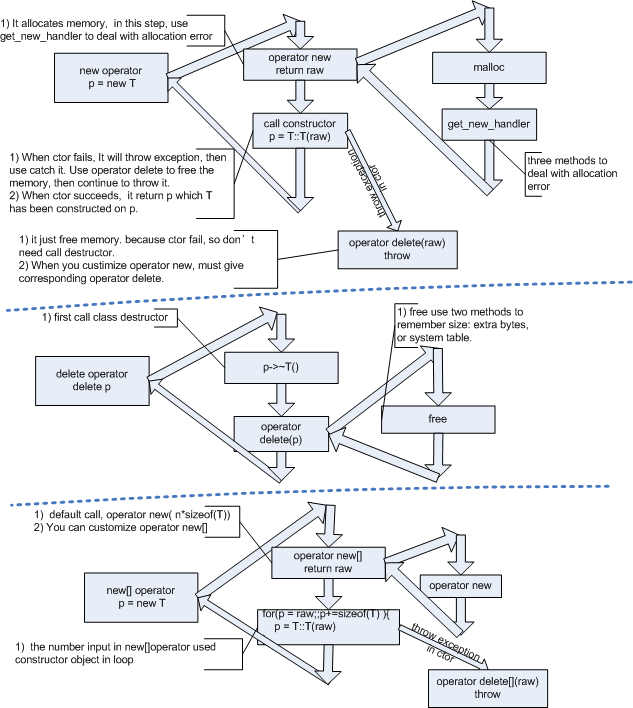
\includegraphics[width=0.90\linewidth]{pics/new.png}
	\caption{new operator and operator new.}
	\label{fig:smartpointer}
\end{figure}


\chapter{Pointer and smart pointer}

\section{pointer and new}

\subsection{When to use pointer?}
\begin{itemize}

    \item When do you use a smart pointer? Here I change this questions to another question, When do you use a pointer?

    \begin{enumerate}

		\item A new object remains in existence, until you delete it. You control the life time of it, maybe you create it in fun1, then delete it in fun4. so the obj is neither stack duration nor static duration. You may or may not transfer \textbf{ownership} between functions. Or when you want to create a obj in runtime according runtime condition or user input dynamically. (maybe don't create it. ) In another word, anyplace where you need object(reference) semnatic, not value semnatic. One example is observer pattern. Below code also demonstrates usage of pointer. \texttt{ToothBrush} need to be control life time and created dynamically.

\begin{lstlisting}[numbers=none]
class Person{
public:
	ToothBrush* pbrush;

	buyNewBrush(string &name){
	    if(pbrush != nullptr}{
		    	delete pbrush;
	    }
	    if(name == "Orlab")
	          pbrush = new Brush();
	    }
	}
	~Person(){
		if(pbrush != nullptr}{
			delete pbrush;
	    }
}

Person Yan();
Yan.buyNewBrush("Oralb");
//......Three months later...........
Yan.buyNewBrush("Philip");
}
\end{lstlisting}

		\item Large array or resources,  if you allocate in stack, it will cause stack overflow. \textbf{In practices, this requirement is deprecated, because any time when you use array [] or new [], you need consider to use std::array or std::vector and std::string instead.} So it's obsolete.

		\item Polymorphism.You can use reference as well if it's just for Polymorphism. So it's obsolete too.

\end{enumerate}

	\item The problem of raw pointer: 1) buffer overrun 2) wild pointer 3) double delete 4) memory leak 5) no matching new and delete 6) fragmentation of memory. For buffer overrun and no matching new and delete, we can use vector/string to resolve this problem. For wild pointer, double delete and memory leak, we can use smart pointer to resolve. With help of smart pointer, the memory can be free immediately, It's very import for performance. For example, if memory looks like this: XXXOXXX, once we free O, then we will have seven continuous memory. Not only free one byte memory, it will produce a bigger chunk of memory for the future allocation, this is very import in memory management. 
\end{itemize}


\section{Basic smart pointer knowledge}

\subsection{Implementation smart pointer?}
\begin{itemize}

		\item A simple \texttt{auto\_ptr} source code: You can learn how to overload \texttt{operator*()} and \texttt{operator->().} \texttt{auto\_ptr} has been deprecated in C++ 17.
\begin{lstlisting}[frame=single, language=c++, mathescape=true]
template <class T> class auto_ptr{
    T* ptr;
public:
    explicit auto_ptr(T* p = 0) : ptr(p) {}
    ~auto_ptr()                 {delete ptr;}
    T& operator*()     {return *ptr;}
    T* operator->()    {return ptr;}
};

auto_ptr<int> aupr;
\end{lstlisting}

\begin{description}
	\item[line 6-7:] Pay attention to the \texttt{operator *} and \texttt{operator ->}. \texttt{operator->} can be overloaded to return another object or pointer. which is then used with operator-> recursively. The statement \texttt{p->m} is interpreted as \texttt{(p.operator->())->m}. 
	
	\item[Line 10:] \texttt{auto\_ptr} is \texttt{nullptr} even you don't initialize it. Smart pointer is \texttt{nullptr} default if you don't initialize. You avoid wild pointer problem.
\end{description}

	\item For \texttt{shared\_ptr}, we need to pay attention to its reference number. 
\begin{lstlisting}[frame=single, language=c++, mathescape=true]
class shared_count {
public:
	shared_count();
	void add_count();
	long reduce_count();
	long get_count() const;
private:
	atomic_int use_count_;
};
\end{lstlisting}

\begin{lstlisting}[frame=single, language=c++, mathescape=true]
template <typename T>
class smart_ptr {
public:  
	...
private:  
	T* ptr_;  
	shared_count* shared_count_;
};
\end{lstlisting}

\begin{description}
	\item[line 7] We can't use \texttt{shared\_count} here. Otherwise, two \texttt{shared\_ptr} will have two separate copy. We can't use \texttt{satic shared\_count} here either. Otherwise, all objects will share the same count. The only practically usage is pointer, this is a object semantic, not a value semantic.  
\end{description}

	\item Four points when you want to implement smart pointer: All these design idea can be used in other context, so you should know it. 

	\begin{enumerate}
		\item \texttt{operator *} and \texttt{operator ->} overload
		\item disable copy and support move constructor
\begin{lstlisting}[frame=single, language=c++, mathescape=true]
smart_ptr(const smart_ptr&)    = delete;  
smart_ptr& operator=(const smart_ptr&)    = delete;
\end{lstlisting}

		\item Implemenation of reference number. 
		
		\item template constructor. it is used to support assignment between child class smart pointer and parent class smart pointer.
		
\begin{lstlisting}[frame=single, language=c++, mathescape=true]
template <typename T>
class unique_ptr{
	.....
	template <typename U>  
	unique_ptr(unique_ptr<U>&& other)  {
		ptr_ = other.release();  
	}
}

unique_ptr<parent> pc{new Child};
unique_ptr<parent> pp{std::move(pc)};
\end{lstlisting}

	\end{enumerate}

\end{itemize}

\subsection{Why need smart pointer?}
\begin{itemize}

		\item Why do we need smart pointer?
\begin{enumerate}
		
\item "Just remember" is seldom the best solution! So we need smart pointer to perform delete operator automatically.

\item When throw an exception, or return in the middle of code. delete will not be invoked at all, It will cause memory leaking. When you use smart pointer, If an exception is thrown in the middle of fun, no memory leak happens.
\begin{lstlisting}[numbers=none]
void methodA() {
   unique_ptr<int> buf(new int[256]);

   int result = fillBuf(buf))
   if(result == -1)
      return;
}
\end{lstlisting}
\begin{description}
	\item[Source code:] You don't need call \texttt{delete} at all. The memory allocated by \texttt{new} will be deleted automatically when \texttt{methodA} finishes.
\end{description}

\item \textbf{smart pointer can manage exclusive or share ownership automatically. }
\end{enumerate}

\item There are four kinds of smart pointer: \texttt{auto\_ptr} \texttt{unique\_ptr} \texttt{shared\_ptr} and \texttt{weak\_ptr}  But only \texttt{unique\_ptr} , \texttt{shared\_ptr} and \texttt{weak\_ptr} are recommended to use.
\begin{enumerate}
	\item  \texttt{auto\_ptr} is now deprecated, and should not be used in new code. When you get a chance, try doing a global search-and-replace of \texttt{auto\_ptr} to \texttt{unique\_ptr} in your code base. 
	
	\item \texttt{weak\_ptr} is mainly used for observer, you can always use raw pointer or reference for this purpose. Raw pointer can't check if pointee object is still valid, \texttt{weak\_ptr} can accomplish this task.
\end{enumerate}

\item Why not recommended \texttt{auto\_ptr} ? When you assign \texttt{targetP = sourceP}, it will cause \texttt{sourceP} set to be \texttt{nullptr}, It causes trouble when you use \texttt{sourceP} in the future. You can't create container includes \texttt{auto\_ptr}, compiler prohibit you from doing so!

\begin{lstlisting}[numbers=none]
auto_ptr<string> ps (new string("hello world") );
auto_ptr<string> ps1;
ps1 = ps;   // ps will be set null.
ps->size() // it will crash the application.

auto_ptr<string> parray[5]; //compiling error.
\end{lstlisting}

\item \textbf{When you construct a smart pointer, you must use 1) a pointer and 2) this pointer must be produced by new.} You can't build smart pointer by address operator, Such as \texttt{unique\_ptr<double> ptr(\&int);}   Why? because smart pointer will call delete when it is out of scope.  delete operator has to be used on pointer produced by new operator.

\item Smart pointer supports flexible operations. Such as obtain the raw pointer \texttt{get}, relinquish control of the pointed object \texttt{release}, and to replace the object it manages \texttt{reset}. Smart pointer has \texttt{bool} operator, you can use if to test if it's nullptr directly.

\begin{lstlisting}[numbers=none]
string * cp = new string("hello world");
shared_ptr<string> ps(cp);
string * cp1 = ps.get(); //use get() get normal pointer.

std::unique_ptr<int> ptr(new int(42));
if (ptr) std::cout <<  *ptr << '\n';
ptr.reset(); //
if (ptr) std::cout <<  *ptr << '\n';
\end{lstlisting}

\item \texttt{shared\_ptr<T>} and \texttt{shared\_ptr<const T>} are not interchangeable. It goes one way - \texttt{shared\_ptr<T>} is convertable to \texttt{shared\_ptr<const T>} but not the reverse.
\begin{lstlisting}[numbers=none]
shared_ptr<int> pint(new int(4)); 
// normal shared_ptr
shared_ptr<const int> pcint = pint; 
// shared_ptr<const T> from shared_ptr<T>
shared_ptr<int> pint2 = pcint; // error! 
\end{lstlisting}

\item Combine smart pointer and \texttt{const}, we can have four different options.
\begin{lstlisting}[numbers = none]
shared_ptr<T> p;        //---> T * p;
const shared_ptr<T> p;   //---> T * const p;
shared_ptr<const T> p;   //---> const T * p;
const shared_ptr<const T> p; //---> const T * const p;
\end{lstlisting}

\end{itemize}

\subsection{unique\_ptr}

\subsubsection{Introduction of unique\_ptr}
\begin{itemize}

\item Create \texttt{unique\_ptr} from new. \textbf{make\_unique is better than inside new, inside new is better than outside new.}
\begin{lstlisting}[frame=single, language=c++]
string * cp = new string("hello world");

unique_ptr<string> ps = cp; // NOT allow to assign unique_ptr directly.
unique_ptr<string> ps (cp); //Ok, not good, outside new.
unique_ptr<string> ps (new string("hello world")); //good , inside new
auto ps( std::make_unique<string>("hello") ); //best, make_unique 
\end{lstlisting}

\item Create \texttt{unique\_ptr} from another \texttt{unique\_ptr}, you have to use move.
\begin{lstlisting}[frame=single, language=c++]
unique_ptr<string> ps1 (new string("hello world"));

unique_ptr<string> ps2 ( ps1 ); //compile error
unique_ptr<string> ps2 ( move(ps1) ); //ok
unique_ptr<string> ps2 = move(ps1) ; //ok
\end{lstlisting}
\begin{description}
	\item[Line 4-5:] ownership transfer from ps1 to ps2, nothing delete. ps1 points a nullptr.
\end{description}

\item When pass \texttt{unique\_ptr} value into a function.
\begin{enumerate}
	\item \textbf{For some exist \texttt{unique\_ptr}, use move to transfer ownership.}
	\item \textbf{For new \texttt{unique\_ptr}, use \texttt{make\_unique} to assure exception safe.}	
\end{enumerate}

\begin{lstlisting}[frame=single, language=c++]
void sink(unique_ptr<widget> arg1, unique_ptr<gadget> arg2);

sink( std::move(exist_uptr_wi), std::move(exist_uptr_ga))

sink(make_unique<widget>(arg1, arg2),make_unique<gadget>(arg1, arg2));  
\end{lstlisting}


\item \texttt{unique\_ptr} operations.
\begin{lstlisting}[frame=single, language=c++]
auto ps1 (make_pair<string>("ps1"));
auto ps2 (make_pair<string>("ps2"));
ps1= ps2; //compile error, not allow

ps1 = std::move(ps2);

ps1.reset(new string("ps3"));

string* pstr = ps1.release();
\end{lstlisting}
\begin{description}
	\item[Line 5:]  Pointer inside previous \texttt{ps1} will be deleted. Pointer inside ps1 point to "ps2" string now. pointer inside ps2 will set to nullptr.
	\item[Line 7:]  Pointer inside previous \texttt{ps1} will be delete.
	
	\item[Line 9:] Use \texttt{pstr} get pointer managed by ps1. Pointer in \texttt{ps1} will be set to nullptr.It's you duty to manage the memory which pointed by pointer pstr.
\end{description} 

\item If a program attempts to assign one \texttt{unique\_ptr} to another. The compiler allows it if the source object is a temporary rvalue (It will call move constructor or assignment of \texttt{unique\_ptr} inside.) and disallows it if the source object has some duration. \textbf{It is a move-only type.}
\begin{lstlisting}[numbers=none]
unique_ptr<string> ps2 = uqique_ptr<string>(new string("yo") );  //compile error here

uqique_ptr<string> fun(){
	return unique_ptr<string> temp(new string("yan");
}
pu2 = fun(); //OK
\end{lstlisting}

\item \texttt{unique\_ptr} supports \textbf{source and sink idiom}.
\begin{lstlisting}[numbers=none]
unique_ptr fun() //support source

fun(unique_ptr up);  //use move to support sink
fun(move(other_up));
\end{lstlisting}

\item Just observer, not transfer ownership , you can get pointer, or use \texttt{unique\_ptr} reference.
\begin{lstlisting}[numbers=none]
unique_ptr<string> ps1 (new string("ps1"));

fun(string* pstr);  //ps1.get()
fun(unique_ptr<string> & ref_ptr);
\end{lstlisting}


\item \texttt{Unique\_ptr} has new [] version. The existence of \texttt{std::unique\_ptr} for arrays should be of only intellectual interest to you, because std::array, std::vector, and std::string are virtually always better data structure choices than raw arrays. About the only situation I can conceive of when a \texttt{std::unique\_ptr<T[]>} would make sense would be when you're using a C-like API that returns a raw pointer to a heap array that you assume ownership of it.
\begin{lstlisting}[numbers=none]
unique_ptr<double []>  pda(new double[5] );
// it will call delete [] inside.
\end{lstlisting}


    \item \texttt{unique\_ptr} can be used inside of class. Below class B disable value-copying (or to define a suitable copy-constructor  and operator= to handle it safely).
\begin{lstlisting}[numbers=none]
class B {  // this class can't be copy
public:
   unique_ptr<int> i;
   B():i(new int(0)) { }
};
\end{lstlisting}

    \item A common use for \texttt{std::unique\_ptr} is as a factory function return type for objects
in a hierarchy. Detail can be seen "effective modern c++ item 18"

\begin{lstlisting}[frame=single, language=c++, mathescape=true]
template<typename... Ts>
auto makeInvestment(Ts&&... params) {
	auto delInvmt = [](Investment* pInvestment) {
		makeLogEntry(pInvestment); // makedelete
		delete pInvestment; // Investment
	};

	std::unique_ptr<Investment, decltype(delInvmt)> pInv(nullptr, delInvmt);
	
	if (...){
		pInv.reset(new Stock(std::forward<Ts>(params)...));
	}
	else if (... ) {
		pInv.reset(new Bond(std::forward<Ts>(params)...));
	}
	return pInv; // as before
}
\end{lstlisting}
\begin{description}
    \item[Source code:] During construction, \texttt{std::unique\_ptr} objects can be configured to use custom deleters: arbitrary functions (or function objects, including those arising from lambda expressions) to be invoked when it's time for their resources to be destroyed. when a custom deleter can be implemented as either a function or a captureless lambda expression, the lambda is preferable. When a custom deleter is to be used, its type must be specified as the second type argument to \texttt{std::unique\_ptr}.
\end{description}

    \item \texttt{std::unique\_ptr} is the C++11 way to express exclusive ownership, but one of its most attractive features is that it easily and efficiently converts to a \texttt{std::shared\_ptr}: This is a key part of why \texttt{std::unique\_ptr} is so well suited as a factory function return type. Factory functions can't know whether callers will want to use exclusive ownership semantics for the object they return or whether shared ownership
\begin{lstlisting}[frame=single, language=c++, mathescape=true]
shared_ptr<Investment> sp=makeInvestment(arguments); 
\end{lstlisting}

    \item Although \texttt{unique\_ptr} has another deleter type, by using an empty deleter object and at the condition that \texttt{unique\_ptr} implementation uses the “Empty Base Optimization” trick, which is usually the case for current STL implementations. By default, \texttt{std::unique\_ptrs} are the same size as raw pointers, so efficiency of it is just like raw pointer.
\begin{lstlisting}[frame=single, language=c++, mathescape=true]
template<class T, 
		class Deleter = std::default_delete<T>
		> class unique_ptr;
\end{lstlisting}

\end{itemize}

\subsubsection{unique\_ptr and container}
\begin{itemize}
\item If a vector contains \texttt{std::unique\_ptr<Fruit>} instead of raw pointers (to prevent memory leaks). vector need copy in and copy out. but \texttt{unique\_ptr} don't support copy. You can use below methods to resolve it.
\begin{enumerate}
	\item you can use \texttt{emplace\_back} with new pointer, but it will lead memory leak if extending vector size fail.
	\item use unname \texttt{unique\_ptr.}
	\item use \texttt{make\_unique}.
\end{enumerate}
\begin{lstlisting}[frame=single, language=c++]
class Fruit { ... };
class Pear : Fruit { ... };
class Tomato : Fruit { ... };

std::vector<std::unique_ptr<Fruit> > m_fruits;
m_fruits.emplace_back(new Pear); //bad method
m_fruits.push_back(std::unique_ptr<Fruit>(new Pear)); //good method
m_fruits.push_back(std::make_unique<Pear>());//best method 
\end{lstlisting}

\item You can sort \texttt{unique\_ptr} objects in an STL container providing you don't invoke methods or algorithm, such as copy(), that copy or assign one \texttt{unique\_ptr} to another.  see "effective STL item 8."

\begin{lstlisting}[numbers=none]
bool compare_by_uniqptr(
               const unique_ptr<SomeLargeData>& a,
               const unique_ptr<SomeLargeData>& b) {
    return a->id < b->id;
}

sort(vec_uni.begin(),vec_uni.end(),compare_by_uniqptr);
\end{lstlisting}

\begin{lstlisting}[frame=single, language=c++]
typedef std::unique_ptr<int> unique_t;
typedef std::vector< unique_t > vector_t;

vector_t vec2(5, unique_t(new Foo));     //Error (Copy)
vector_t vec3(vec1.begin(), vec1.end()); //Error (Copy)
std::copy(vec1.begin(), vec1.end(),
          std::back_inserter(vec2)); // Error (copy)

vector_t vec3(make_move_iterator(vec1.begin()),
                 make_move_iterator(vec1.end())); //Ok

std::sort(vec1.begin(), vec1.end());
\end{lstlisting}

\end{itemize}


\subsection{shared\_ptr}
\begin{itemize}
\item Every \texttt{shared\_ptr} has a control block in side of it. \textbf{When are control blocks created?}  It's very important conception, when you understand it, you will know what happen when you create or assign a \texttt{shared\_ptr} better. 
\begin{center}
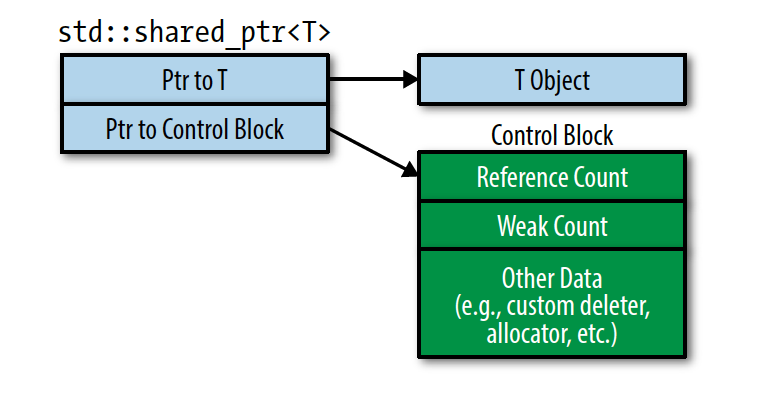
\includegraphics[scale=0.6]{pics/shared.png}
\end{center}


\begin{enumerate}
	\item \texttt{std::make\_shared}  always creates a control block. It manufactures a new object to point to, so there is certainly no control block for that object at the time \texttt{std::make\_shared} is called.
	
	\item A control block is created when a \texttt{std::shared\_ptr} is constructed from a unique-ownership pointer (i.e., a \texttt{std::unique\_ptr} ). As part of its construction, the \texttt{std::shared\_ptr} assumes ownership of the pointed-to object, so the unique ownership pointer is set to null.
	
	\item When a \texttt{std::shared\_ptr} constructor is called with a raw pointer, it creates a control block.
	
	\item \texttt{std::shared\_ptr} constructors taking \texttt{std::shared\_ptrs} or \texttt{std::weak\_ptrs} as constructor arguments. \textbf{NOT} create new control blocks, because they can rely on the smart pointers passed to them to point to any necessary control blocks
	
\end{enumerate}

	
    \item Create \texttt{shared\_ptr} from new. \textbf{\texttt{make\_shared} is better than inside new, inside new is better than outside new.}
\begin{lstlisting}[frame=single, language=c++]
string * cp = new string("hello world");

shared_ptr<string> ps = cp; //NOT allow

shared_ptr<string> ps (cp); //outsie new 
shared_ptr<string> ps (new string("hello world")); //inside new,good style
unique_ptr<string> ps( std::make_shared<string>("hello world") ); //make, best style
\end{lstlisting}

    \item First, try to avoid passing raw pointers to a \texttt{std::shared\_ptr} constructor. 1) use \texttt{make\_shared}. 2) if you have custom deleter and can't use \texttt{make\_share()}.  Pass the result of new directly instead of going through a raw pointer variable.

\begin{lstlisting}[frame=single, language=c++]
auto pw = new Widget; // pw is raw ptr

std::shared_ptr<Widget> spw1(pw, loggingDel);
std::shared_ptr<Widget> spw2(pw, loggingDel);
\end{lstlisting}
\begin{description}
	\item[line 3:] create control block for \texttt{*pw}.
	\item[Line 4:] create 2nd control block for \texttt{*pw}! BAD! That will cause undefine result!
\end{description}

\item Create \texttt{shared\_ptr} from another \texttt{shared\_ptr}.
\begin{lstlisting}[frame=single, language=c++, mathescape=true]
shared_ptr<string> ps1 (new string("hello world"));
shared_ptr<string> ps2 ( ps1 );
shared_ptr<string> ps2 ( move(ps1) );
\end{lstlisting}
\begin{description}
	\item[Line 2:] use\_count of \texttt{ps1} and \texttt{ps2} are all 2, and they share the same use\_count.
	\item[Line 3:] the original \texttt{ps1} will become null, and the reference count does not get modified. Just transfer use\_count to \texttt{ps2}. 
\end{description}

    \item \texttt{shared\_ptr} assignment.
\begin{lstlisting}[frame=single, language=c++, mathescape=true]
shared_ptr<string> ps1 (new string("ps1"));
shared_ptr<string> ps2 (new string("ps2"));

ps1 = ps2;
ps1 = std::move(ps2);
ps1.reset(cp); 
\end{lstlisting}
\begin{description}
	\item[Line 4:] Use assignment  1) In \texttt{ps1}, previous use\_count decrements 1(If equal 0, will delete) 2) \texttt{ps1} points to current use\_count 3) and current use\_count increments 1
	
	\item[Line 5:] Use move 1) In \texttt{ps1}, previous use\_count decrements 1(If equal 0, will delete) 2) \texttt{ps1} points to current use\_count 3) \texttt{ps2} is null now. 
	
	\item[Line 6:] Use \texttt{reset}. pointer inside previous \texttt{ps1} will decrement 1. by now, current \texttt{ps1} reference count will be 1.
\end{description}

\begin{figure}[h]
	\centering
	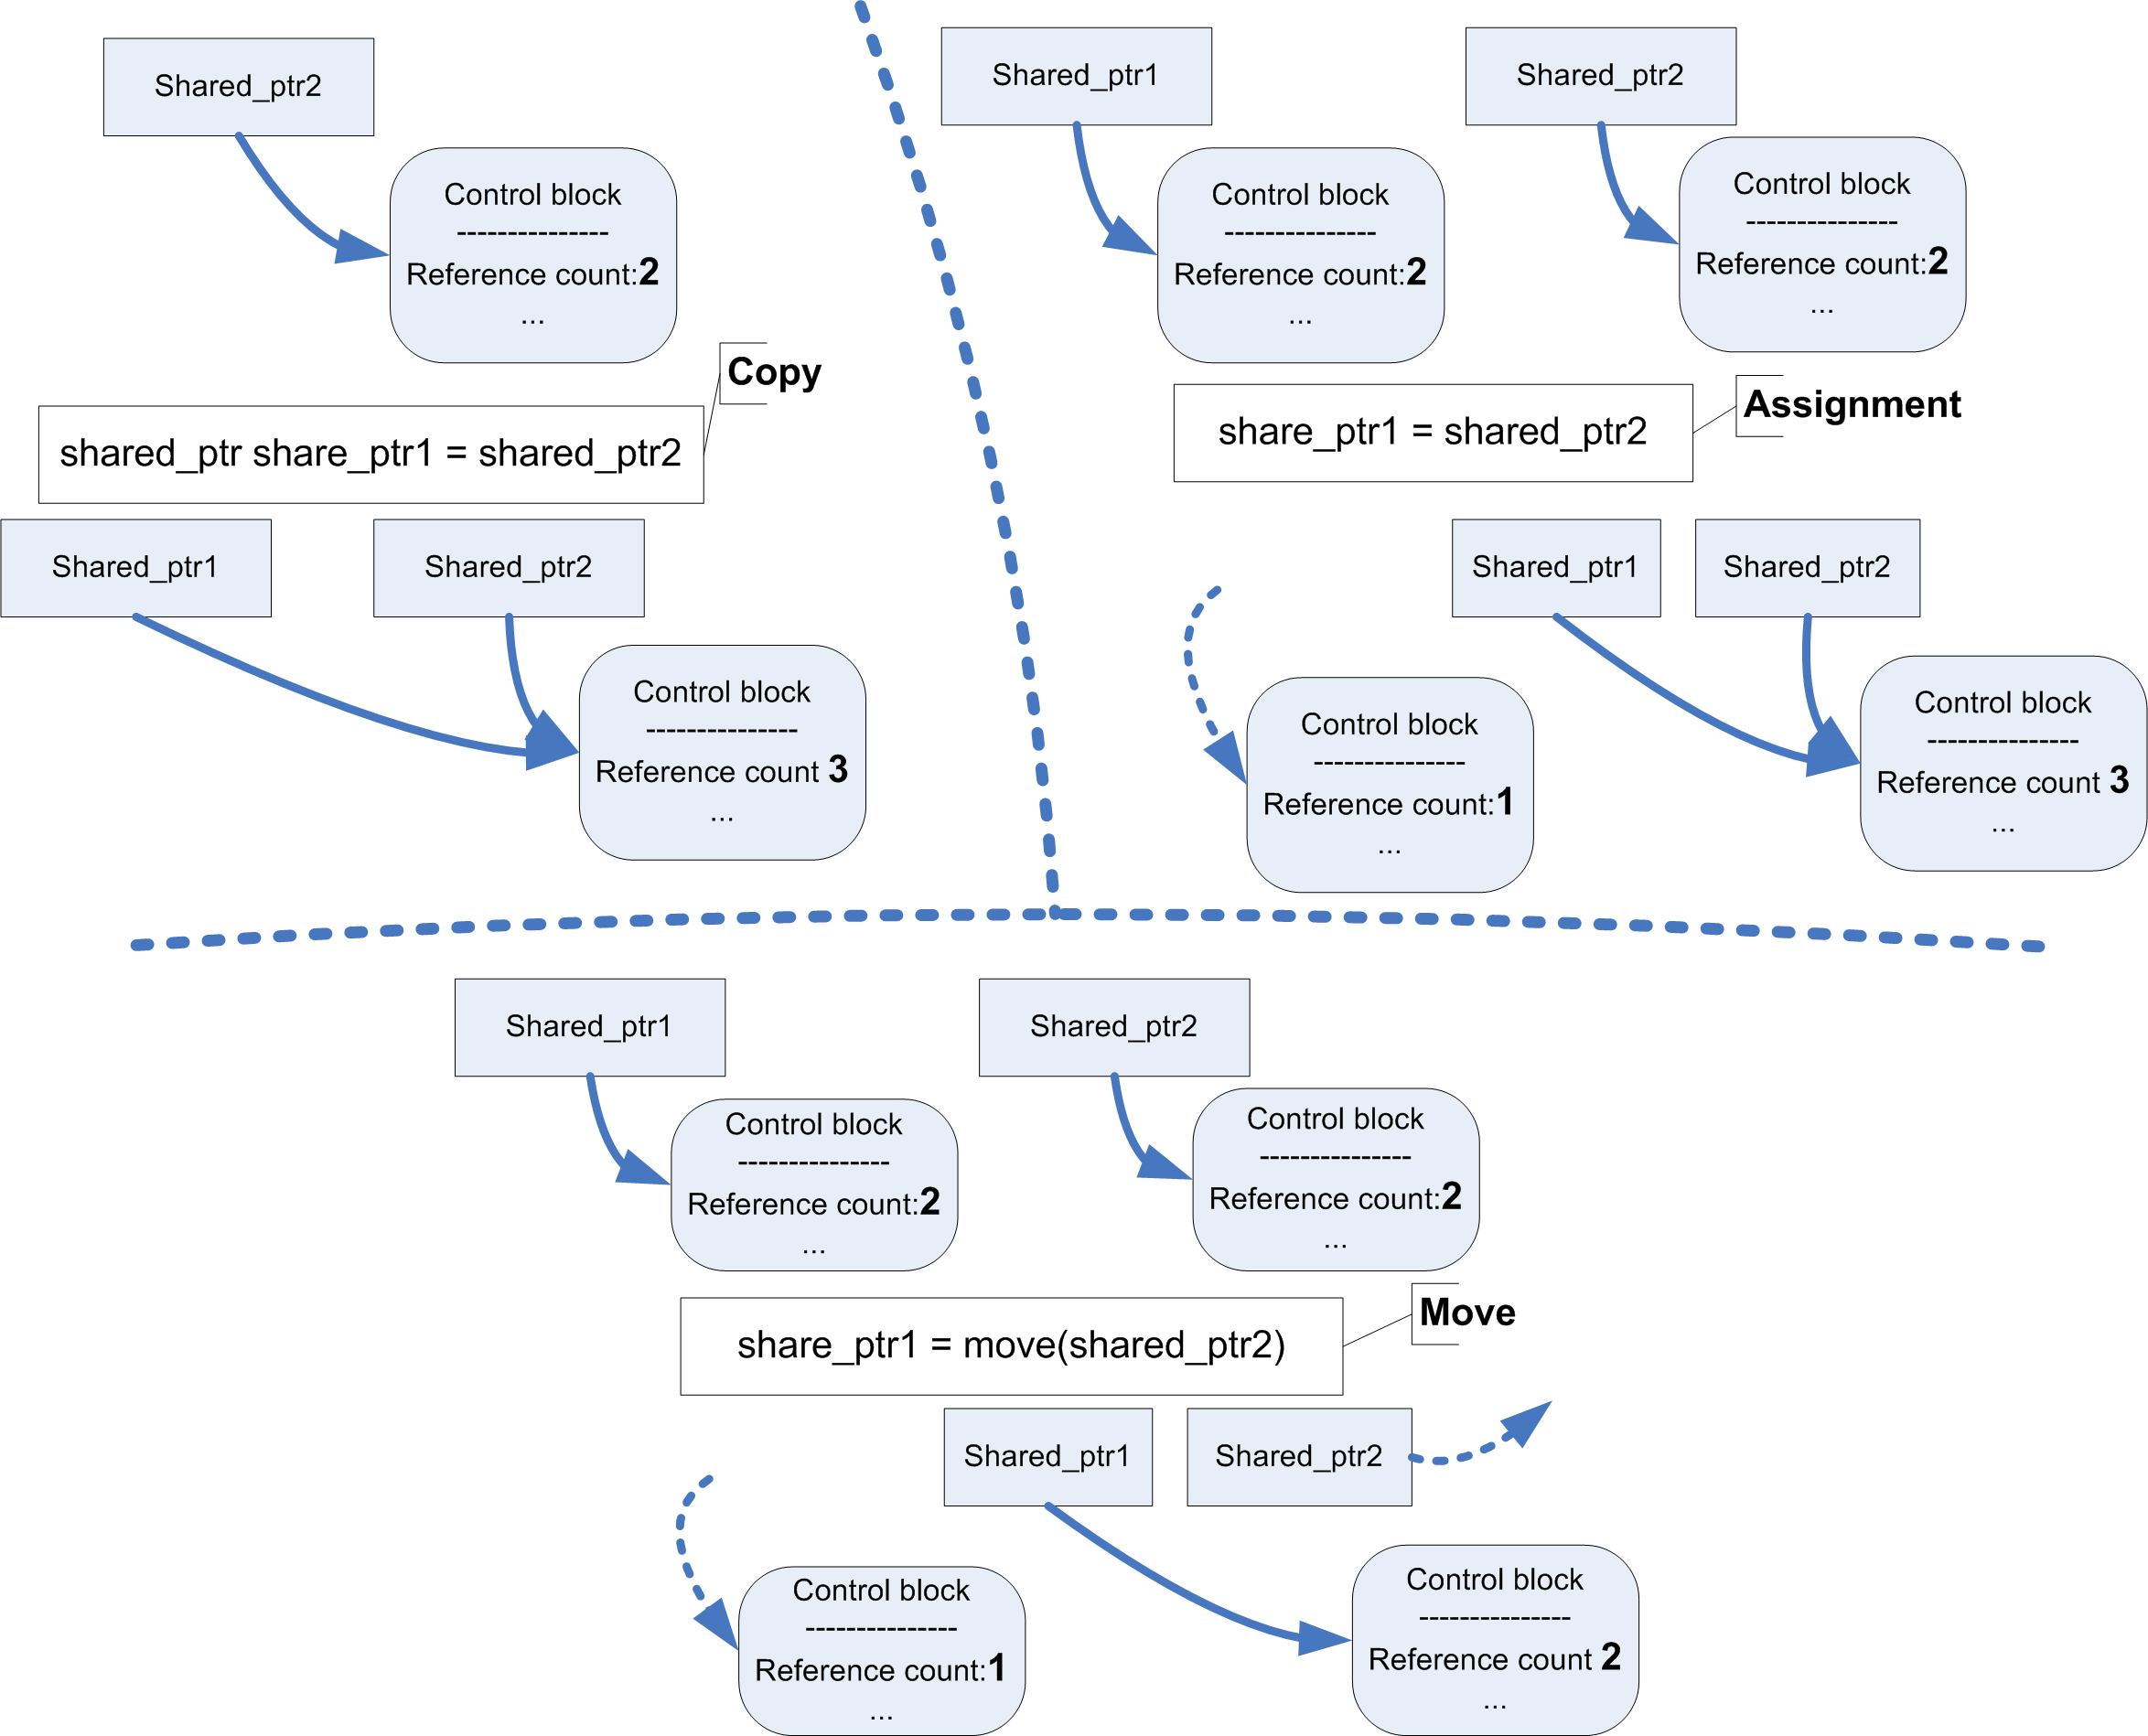
\includegraphics[width=0.9\linewidth]{pics/shared_ptr.png}
	\caption{Difference between copy, assignment and move.}
	\label{fig:sharedptr}
\end{figure}


\item Difference between constructor and assignment.
\begin{enumerate}
\item When assignment, previous decrements 1 and current increment 1;
\item When copy constructor, current increment 1;
\item When constructor from raw pointer, current is 1;
\end{enumerate}

\item Just observer, not transfer ownership , you can get pointer, or use \texttt{shared\_ptr} reference. 
\begin{lstlisting}[numbers = none]
shared_ptr<string> ps1 (new string("ps1"));

fun(string* pstr);
fun(shared_ptr<string>& ref_ptr);
\end{lstlisting}


\item Like \texttt{std::unique\_ptr}, \texttt{std::shared\_ptr} uses delete as its default resource-destruction mechanism, but it also supports custom deleters.
\begin{lstlisting}[frame=single, language=c++]
auto loggingDel = [](Widget *pw){ // custom deleter
	makeLogEntry(pw);
	delete pw;
};

std::unique_ptr< Widget, decltype(loggingDel) > upw(new Widget, loggingDel);

std::shared_ptr<Widget> spw(new Widget, loggingDel);
\end{lstlisting}
\begin{description}
	\item[Line 6:] deleter type is ptr type
	\item[Line 8:] deleter type is not part of ptr type. \texttt{shared\_ptr} use type erase technique, which is introduced in "Generic programming" section. 
\end{description}

\item In order to correctly use \texttt{shared\_ptr} with an array, you must supply a custom deleter. But we don't recommend using \texttt{shared\_ptr} with array. \textbf{Any time you new a array, you should first consider using STL container directly.}
\begin{lstlisting}[numbers=none]
template< typename T >
struct array_deleter {
  void operator ()( T const * p){
    delete[] p;
  }
};

shared_ptr<int> sp(new int[10],array_deleter<int>());
\end{lstlisting}

\item Usage of \texttt{enable\_shared\_from}. If you don't use it, multiple distinct \texttt{shared\_ptr} objects with separate reference counts. For this reason you must never create more than one \texttt{shared\_ptr} \textbf{from the same raw pointer.} It has become C++11 standard.
\begin{lstlisting}[frame=single, language=c++]
class Test : public boost::enable_shared_from_this<Test> {
public:
    boost::shared_ptr<Test> GetObject()
    {
        return shared_from_this();
        //return shared_ptr<test>(this);
    }
};
int main(int argc, char *argv[]){
    boost::shared_ptr<Test> p( new Test( ));
    boost::shared_ptr<Test> q = p->GetObject();
}
\end{lstlisting}
\begin{description}
	\item[Line 6:] You can't do this way if you create \texttt{shared\_ptr} from this.
\end{description}

\end{itemize}


\subsection{weak\_ptr}
\begin{itemize}

    \item The relationship begins at birth. \texttt{std::weak\_ptrs} are typically created from \texttt{std::shared\_ptrs}. You can only create a \texttt{weak\_ptr} out of a \texttt{shared\_ptr} or another \texttt{weak\_ptr}. A truly smart pointer would deal with this problem by tracking when it dangles, i.e., when the object it is supposed to point to no longer exists. That's precisely the kind of smart pointer \texttt{std::weak\_ptr} is. \textbf{You can't test if a raw pointer is dangle or not.}

    \item \texttt{std::weak\_ptrs} can't be dereferenced, nor can they be tested for nullness. That's because \texttt{std::weak\_ptr} isn't a standalone smart pointer. It's an augmentation of \texttt{std::shared\_ptr}. Almost the only things you can do are to interrogate it to see if the managed object is still there, or construct a \texttt{shared\_ptr} from it.

\begin{lstlisting}[frame=single, language=c++,mathescape=true]
auto spw = std::make_shared<Widget>();
std::weak_ptr<Widget> wpw(spw);
...
spw = nullptr;
if (wpw.expired())
\end{lstlisting}
\begin{description}
	\item[Line 1:] the pointed-to Widget's ref count RC(reference count) is 1.
	\item[Line 2:] \texttt{wpw} points to same Widget as spw. RC remains 1
	\item[Line 5:] RC goes to 0, and the Widget is destroyed. \texttt{wpw} now dangles and doesn't point to an object.
\end{description}

    \item \texttt{lock()} method creates a new \texttt{std::shared\_ptr} that shares ownership of the managed object. If there is no managed object, then the returned \texttt{shared\_ptr} also is empty.

\begin{lstlisting}
std::shared_ptr<Widget> spw1 = wpw.lock(); //if wpw's expired, spw1 is null
auto spw2 = wpw.lock(); //same as above, but uses auto
std::shared_ptr<Widget> spw3(wpw); //if wpw expired, throw std::bad_weak_ptr.
\end{lstlisting}

    \item Potential use cases for \texttt{std::weak\_ptr} includes: caching, observer lists, and the prevention of \texttt{std::shared\_ptr} cycles.  All the detail can be seen in "Effective Modern ++" Item 20.
\begin{lstlisting}[frame=single, language=c++]
std::shared_ptr<const Widget> fastLoadWidget(WidgetID id){
	static std::unordered_map<WidgetID, std::weak_ptr<const Widget>> cache;
	auto objPtr = cache[id].lock();

	if (!objPtr) { // if not in cache,
		objPtr = loadWidget(id); // load it
		cache[id] = objPtr; // cache it
	}
	return objPtr;
}
\end{lstlisting}
\begin{description}
	\item[Line 5:] objPtr is \texttt{std::shared\_ptr} to cached object . (or null if object's not in cache). For above requirement, you also can use raw pointer, But for raw pointer, you can't detect if original one has been delete. 
\end{description}

    \item An example of \texttt{shared\_ptr} cyclic dependency problem. Below code has memeory leak. \texttt(A) and \texttt{B} doesn't have chance to call destructor.
\begin{lstlisting}[]
class B;
class A {
    shared_ptr<B> sP1; // use weak_ptr instead to avoid CD
public:
    A() {  cout << "A()" << endl; }
    ~A() { cout << "~A()" << endl; }
    void setShared(shared_ptr<B>& p) {
        sP1 = p;
    }
};
class B {
    shared_ptr<A> sP1;
public:
    B() {  cout << "B()" << endl; }
    ~B() { cout << "~B()" << endl; }
    void setShared(shared_ptr<A>& p) {
        sP1 = p;
    }
};
int main() {
    shared_ptr<A> aPtr(new A);
    shared_ptr<B> bPtr(new B);
    aPtr->setShared(bPtr);
    bPtr->setShared(aPtr);
}
\end{lstlisting}

\end{itemize}

\subsection{make function}

\begin{itemize}
	\item \textbf{Never say new in c++14!} Prefer to use make function instead of new operator. Don't use \texttt{make\_unique} if you need a custom deleter or are adopting a raw pointer from elsewhere. And \texttt{make\_unique} doesn't joined the Standard Library until c++14.
	
	\item \texttt{make\_unique} just perfect-forwards its parameters to the constructor of the object being created, constructs a \texttt{std::unique\_ptr} from the raw pointer new produces, and returns the \texttt{std::uniqu\_ptr} so created.
	
	\item \texttt{std::make\_unique} and \texttt{std::make\_shared} are two of the three make functions: functions that take an arbitrary set of arguments, perfect-forward them to the constructor for a dynamically allocated object, and return a smart pointer to that object. The third make function is \texttt{std::allocate\_shared}
	
	\item make function has tree advantage: simply, exception safety and allocate once for efficiency.
	
	\begin{enumerate}
		\item The method of using new repeat the type being created, but the make functions don't.That's way make function is better than using \texttt{new}. See the comparison in below source code. 
\begin{lstlisting}[frame=single, language=c++, mathescape=true]
auto upw1(std::make_unique<Widget>()); // better
std::unique_ptr<Widget> upw2(new Widget); 
		
auto spw1(std::make_shared<Widget>()); // better
std::shared_ptr<Widget> spw2(new Widget); 
\end{lstlisting}
		
		\item The second reason to prefer make functions has to do with exception safety. It's obvious that this code entails a memory allocation, but it actually performs two. Item 19 explains that every \texttt{std::shared\_ptr} points to a control block containing, among other things, the reference count for the pointed-to object. That's because \texttt{std::make\_shared} allocates a single chunk of memory to hold both the Widget object and the control block.
		
	\end{enumerate}
	
	\item make function has its limitation:
	\begin{enumerate}
		\item For example, none of the make functions permit the specification of custom deleter.
		
		\item the perfect forwarding code uses parentheses, not braces. The bad news is that if you want to construct your pointed-to object using a braced initializer, you must use new directly. Using a make function would require the ability to perfect-forward a braced initializer, but, as "Effeictive Modern C++"Item 30 explains, braced initializers can't be perfect-forwarded.
\begin{lstlisting}
template<typename T>
void f(T para);

f({1,2,3}) //error, can't deduce type T

template<typename T>
void f(std::initializer_list<T> initList);
f({1,2,3}) //OK.
\end{lstlisting}

\begin{lstlisting}
auto upv = std::make_unique<std::vector<int>>(10, 20);
auto initList = { 10, 20 };
auto spv = std::make_shared<std::vector<int>>(initList);
\end{lstlisting}
\begin{description}
	\item[Line 1:] upv has 10 elements, each one is 20.
	\item[Line 2:] create \texttt{std::initializer\_list}
	\item[Line 3:] create \texttt{std::vector} using \texttt{std::initializer\_list} constructor
\end{description}
		
		\item As long as \texttt{std::weak\_ptrs} refer to a control block (i.e., the weak count is greater than zero), that control block must continue to exist. And as long as a control block exists, the memory containing it must remain allocated. The memory allocated by a \texttt{std::shared\_ptr} make function, then, can't be deallocated until the last \texttt{std::shared\_ptr} and the last \texttt{std::weak\_ptr} referring to it have been destroyed
	\end{enumerate}
	
	\item If you can't use make function, you have to create \texttt{shared\_ptr} first, then pass it to function, but a better way is to move it.
\begin{lstlisting}[frame=single, language=c++]
std::shared_ptr<Widget> spw(new Widget, cusDel);
processWidget(spw, computePriority()); 
// correct, but not optimal; 

processWidget(std::move(spw),computePriority());  
// both efficient and exception safe
\end{lstlisting}
	
\end{itemize}

\subsection{wrapping non-pointer resource in smart pointer}

\subsubsection{Customize deleter in unique\_ptr and shared\_ptr}

\begin{itemize}
	\item For \texttt{uniqu\_ptr}, template has two template parameters: the type of the pointee, and the type of the deleter. This second parameter has a default value, so you usually just write something like \texttt{std::unique\_ptr<int>}.
\begin{lstlisting}
template <
class T,
class Deleter = std::default_delete<T>
> class unique_ptr;
	\end{lstlisting}

	\item What is best to use as a deleter? let's consider the following options:
	\begin{enumerate}
		\item std::function - heavy stuff, on 64 bit, gcc it showed me 40 bytes.
		
		\item Function pointer - it’s just a pointer, so now \texttt{unique\_ptr} contains two pointers: for the object and for that function… so 2*sizeof(ptr) = 8 or 16 bytes.
		
		\item \textbf{Stateless functor (and also stateless lambda)} - it’s actually very tricky thing. You would probably say: two pointers… but it’s not. Thanks to empty base optimization - EBO the final size is just a size of one pointer, so the smallest possible thing.
		
		\item State-full functor - if there is some state inside the functor then we cannot do any optimizations, so it will be the size of ptr + sizeof(functor)
		
		\item Lambda (statefull) - similar to statefull functor
	\end{enumerate}

	\item You can see for stateless functor or lambda, the size is just one pointer, we don't need pay and space fee. That is why we \texttt{unique\_ptr} has two template parameter, and one you can specify the deleter type. if deleter type is empty stateless functor, size will be just one pointer. 
	
	
	\item If you don't care space, but flexibility,(You want to pass any type caller-able object).  You can always add your own type erasure on top by using std::function. For example, you can have \texttt{unique\_ptr<T, std::function<void(T*)> >}.
	
	\item Guideline: Use \texttt{make\_unique} to create an object that is not shared (at least not yet), unless you need a custom deleter or are adopting a raw pointer from elsewhere.
	
\begin{lstlisting}[frame=single, language=c++]
typedef struct {
	//...
} Foo;

Foo* createObject(int i_val, double d_val) {
	Foo* output = (Foo*)malloc(sizeof(Foo));
	return output;
}
struct FooDeleter {
	void operator()(Foo* p) const {
		destroy(p);
	}
};
	
using FooWrapper = std::unique_ptr<Foo, FooDeleter>;
FooWrapper foo(createObject(32, 3.14));
\end{lstlisting}

	\item The \texttt{std::shared\_ptr} template has only one parameter though: the type of the pointee. But you can use a custom deleter with this one too, even though the deleter type is not in the class template. \textbf{shared\_ptr and std::functions use type erase technology.} you can see the type erase technology in generic programming chapter later.
\begin{lstlisting}
template< class T > class shared_ptr;
\end{lstlisting}
	
	\item Part of the reason is that \texttt{shared\_ptr} needs an explicit control block anyway for the ref count and sticking a deleter in isn't that big a deal on top. \texttt{unique\_ptr} however doesn't require any additional overhead, and adding it would be unpopular- it's supposed to be a zero-overhead class. \texttt{unique\_ptr} is supposed to be static. 
\begin{lstlisting}[frame=single, language=c++]
typedef struct {
	//...
} Foo;

Foo* createObject(int i_val, double d_val) {
	Foo* output = (Foo*)malloc(sizeof(Foo));
	return output;
}

void destroy(Foo* obj) {
	free(obj);
}

std::shared_ptr<Foo> foo(createObject(32, 3.14), destroy);
\end{lstlisting}
\end{itemize}

\subsubsection{Customize resource type}
\begin{itemize}
		\item For \texttt{unique\_ptr}, if you can deduct pointer type from deleter, \texttt{unique\_ptr} will use it directly, so you just know SC\_HANDLE is a kind of "pointer", but you don't know exact type, you can write just like below.  That is because in \texttt{unique\_ptr}, If you provide and deleter and inside deleter, you also provide pointer type. If that type exists, we use this as resource type, otherwise \texttt{T*}. Must satisfy NullablePointer.

\begin{lstlisting}[frame=single, language=c++]
struct SvcHandleDeleter{
	typedef SC_HANDLE pointer;
	SvcHandleDeleter() {};
	
	void operator()(pointer h) const {
		CloseServiceHandle(h);
	}
};
	
typedef std::unique_ptr<SC_HANDLE,SvcHandleDeleter> unique_sch;
//Pay attention, because you define pointer in side the deleter, 
//so we use SC_HANDLE, not SC_HANDLE* 
	
unique_sch scm(::OpenSCManagerA(0, 0, SC_MANAGER_ALL_ACCESS));
\end{lstlisting}
	
	\item For shared pointer, type-erasure makes it impossible with the current interface to achieve exactly what type you want. So you can use a dumb way, Just like a pointer to pointer. If you don't know what is behind SC\_HANDLE. If you know it's type is void, you can use void directly, it will save you a lot of trouble. 
	
\begin{lstlisting}[frame=single, language=c++]
std::shared_ptr<SC_HANDLE> sp(new SC_HANDLE(
              ::OpenSCManagerA(0, 0, SC_MANAGER_ALL_ACCESS)),
	[](SC_HANDLE* p){ ::CloseServiceHandle(*p); delete p; });
\end{lstlisting}

		\item Different with previous example, if you know \textbf{HANDLE in windows is just void* type pointer}, so you can use this way to deal with windows handle.
	
\begin{lstlisting}[frame=single, language=c++]
struct HANDLEDeleter{
	void operator()(HANDLE handle) const{
		if (handle != INVALID_HANDLE_VALUE)
		CloseHandle(handle);
	}
};
	
using HANDLE_unique_ptr=unique_ptr<void, HANDLEDeleter>;
	
HANDLE_unique_ptr make_HANDLE_unique_ptr(HANDLE handle){ ...
	return HANDLE_unique_ptr(handle);
}
	
auto hInputFile = make_HANDLE_unique_ptr(
                            CreateFile(strIn, GENERIC_READ, ...));
\end{lstlisting}
	
	\item Use \texttt{shared\_ptr} to wrap a handle, A good introduction is "Making a HANDLE RAII-compliant using \texttt{shared\_ptr} with a custom deleter" in stackoverflow

	\item We can \texttt{make FILE*} smart, use \texttt{unique\_ptr} source semantic.
\begin{lstlisting}[frame=single, language=c++]
struct FILEDeleter {
	void operator()(FILE *pFile){
		if (pFile)
			fclose(pFile);
		}
};
	
using FILE_unique_ptr = unique_ptr<FILE, FILEDeleter>;
	
FILE_unique_ptr make_fopen(
			const char* fname, const char* mode){
	FILE *fileHandle= nullptr;
	auto err = fopen_s(&fileHandle , fname, mode); 
	if (err != 0){
		return nullptr;
	} 
		return FILE_unique_ptr(fileHandle);
}
	
FILE_unique_ptr pFilePtr = make_fopen("test.txt", "rb");
\end{lstlisting}
	
\item Just the same idea, if you want to use \texttt{shared\_ptr} wrap \texttt{FILE*}, see below example.
\begin{lstlisting}[frame=single, language=c++]
using FILE_shared_ptr = std::shared_ptr<FILE>;
	
FILE_shared_ptr make_fopen_shared(const char* fname, const char* mode){
	FILE *fileHandle = nullptr;
	auto err = fopen_s(&fileHandle, fname, mode);
	if (err != 0){
		return nullptr;
	}
	return FILE_shared_ptr(fileHandle, FILEDeleter());
}
\end{lstlisting}
\begin{description}
	\item[Line 9:] Pay attention!, use FILEDeleter()(That is variable), but unique\_ptr use FILEDeleter(That is type.)
\end{description}

	\item For fstream, it's different with FILE*. It's based on value semantic and it's RAII itself. If you want to share the ownership, you can pass reference directly.Because it doesn't support copy.

\begin{lstlisting}[numbers=none]
fp = fstream(name,mode)};
setLogFile(ifstrea& );
setLogFile(fp);
\end{lstlisting}

\end{itemize}

\section{Smart pointer usage}
\subsection{smart pointer and polymorphism}

\subsubsection{pointer\_cast function}
\begin{itemize}
	\item \textbf{Basic idea: smart pointer base and smart pointer derived are not covariant at all. You can think that just like vector<Base> and vector<derived>}.
			
	\item Even \texttt{DerivedClass} inherit \texttt{BaseClass,}  You can't cast \texttt{shared\_ptr<DerivedClass>} to \newline 
	\texttt{shared\_ptr<BaseClass>} because there is no inheritance relationship between the types. 
	
	\item The \texttt{shared\_ptr<T>(const shared\_ptr<Y>\&)} constructor doesn't help because it is only usable if Y* is implicitly convertible to T*, i.e. it is there to support the same pointer conversions as would happen implicitly, like \texttt{DerivedClass*} to \texttt{BaseClass*,} not \texttt{BaseClass*} to \texttt{DerivedClass*}. That is why we need \texttt{static\_pointer\_cast}.
\begin{lstlisting}
template< class T, class U > 
std::shared_ptr<T> static_pointer_cast( const std::shared_ptr<U>& r ) noexcept {
    auto p = static_cast<typename std::shared_ptr<T>::element_type*>(r.get());
    return std::shared_ptr<T>{r, p};
}
\end{lstlisting}
\begin{description}
	\item[Line 4:] That is called Aliasing \texttt{shared\_ptr} constructor, detail can be google "std::shared\_ptr's secret constructor"
\end{description}

	\item An example of \texttt{static\_pointer\_cast}.
\begin{lstlisting}
struct BaseClass {};

struct DerivedClass : BaseClass {
	void f() const {
		std::cout << "Sample word!\n";
	}
};

int main() {
	std::shared_ptr<BaseClass> ptr_to_base(make_shared<DerivedClass>());
	std::static_pointer_cast<DerivedClass>(ptr_to_base)->f();
	std::dynamic_pointer_cast<DerivedClass>(ptr_to_base)->f();
	static_cast<DerivedClass*>(ptr_to_base.get())->f(); //Error
}
\end{lstlisting}

\end{itemize}

\subsubsection{Four casts in polymorphism}
\begin{itemize}
\item In this section, you need to know four things:
\begin{enumerate}
\item \texttt{share\_ptr} child to base;
\item \texttt{share\_ptr} base to child (down cast);
\item \texttt{unique\_ptr} child to base;
\item \texttt{unique\_ptr} base to child (down cast);
\end{enumerate}

		\item For \texttt{shared\_ptr}, it support derived to base \texttt{shared\_ptr} copy or assignment. Behind the hood, you need to know the template member function. Detail can be found in effective C++ item 45 "Use member function templates to accept "all compatible types". Why you can? because it get raw pointer and wrapped it again and compiler allow it.

		\item  For \texttt{shared\_ptr} base, you can't assign it to the \texttt{shared\_ptr} child, so you must use \\ \texttt{static\_pointer\_cast} and \texttt{dynamic\_pointer\_cast}. They only support \texttt{shared\_ptr}. They use \texttt{shared\_ptr} aliasing constructor, get raw pointer, use static or dynamic cast, then build derived \texttt{shared\_ptr} too. Detail can be found: \\
			"std::static\_pointer\_cast vs static\_cast<std::shared\_ptr<A > >"

		\item If you don't want to shared ownership, but just want to be a observer, you can use reference, but for \texttt{shared\_ptr} base reference, You have to use const. Why do we need const?
	
\begin{lstlisting}[frame=single, language=c++, mathescape=true]
void doSomething(const std::shared_ptr<Base>& ptr) {
    std::cout<<ptr.use_count()<<std::endl; 
}

std::shared_ptr<Derived1> pd1 = std::make_shared<Derived1>();
//doSomething(pd1);  Will not compile here.
doSomething(shared_ptr<Base> temp(pd1));
doSomething(static_pointer_cast<Base>(pd1));
\end{lstlisting}
	\begin{description}
	\item[Line 7:] from pd1 build temporary base \texttt{shared\_ptr} pointer.
	\item[Line 8:] \texttt{static\_pointer\_cast} also return a temporary base \texttt{shared\_ptr}. That is why you need \texttt{const} in line 1
\end{description}


\item static cast also can used for check down cast, it will check at compile time, so sometimes it will fail. Not like dynamic cast, it will check at run time and also require class has at lease one virtual function. Detail can be found in previous chapter. The basic idea is just like \texttt{static\_cast} and \texttt{dynamic\_cast}.

\item For \texttt{unique\_ptr}, You can use move from derived pointer to base pointer directly.
\begin{lstlisting}[frame=single, language=c++, mathescape=true]
void doSomething(const std::unique_ptr<Base> ptr) {
    ptr->run();
}

int main() {
    std::unique_ptr<Derived1> pd1 = std::make_unique<Derived1>();
    doSomething(std::move(pd1));
}
\end{lstlisting}

\item For down cast \texttt{unique\_ptr}, There are no counter part of \texttt{static\_pointer\_cast}. So only way you can do is use release and wrap it again.

\begin{lstlisting}[frame=single, language=c++, mathescape=true]
template<typename TO, typename FROM>
unique_ptr<TO> static_unique_pointer_cast (unique_ptr<FROM>&& old){
	return unique_ptr<TO>{static_cast<TO*>(old.release())};
	//conversion: unique_ptr<FROM>->FROM*->TO*->unique_ptr<TO>
}

unique_ptr<Base> foo = fooFactory();
unique_ptr<Derived> foo2 = 
              static_unique_pointer_cast<Derived>(std::move(foo));
\end{lstlisting}

\item For const reference, there are three methods: 1) Use move 2) Change function interface 3) Change parameter.
\begin{lstlisting}[frame=single, language=c++, mathescape=true]
void f(const unique_ptr<Base>& base)

unique_ptr<Derived> derived = unique_ptr<Derived>(new Derived);
f(derived); //this fail;

f(std::move(derived)); //method 1 work, Why?
    //because int i = 3; const float& dr = i; compile OK
                       
void f(std::unique_ptr<Derived> const&); //method 2, Change function interface

std::unique_ptr<base> derived = std::make_unique<Derived>();//method 3, Change parameter.
std::unique_ptr<base> derived(new Derived);
\end{lstlisting}


\item \textbf{There are three places you can use smart pointer: braced scope(function), class member and container item.} In these three places, you can have exclusive ownership, shared ownership or observer. In the next two sections, I will mainly introduce the relationship between smart pointer and class; relationship between smart pointer and functions.

\end{itemize}


\subsection{Smart pointer and class}
\subsubsection{Semantic of RAII}

\begin{itemize}
		\item The basic idea of RAII is to represent a resource by a local object, so that the local object's destructor will release the resource.  That is to say: To prevent resource leaks, use RAII objects that acquire resources in their constructors and release them in their destructors.
\begin{lstlisting}[numbers = none]
//C version,
File* fp = fopen("/path/to/file");
// throw exception here, then resource leaking
fclose(fp);
	
try { //Java version
	File file = new File("/path/to/file");
	// throw exception here, go to finally.
} finally {
	file.close();
}
\end{lstlisting}
	
\begin{lstlisting}[frame=single, language=c++]
fun{ //c++ version
	fstream if("path/to/file")
	if.getline
	// you don't need to if.close().
}
	
std::unique_ptr<FILE, int(*)(FILE*)> 
	myFile( fopen("myfile", "rb"), fclose );              
\end{lstlisting}

\begin{description}
	\item[Line 7] use smart pointer to wrap FILE* in C language. the custom deleter type: fclose(). (FILE*) is returned by fopen() prototype. the deleter function: fclose() 
\end{description}
			
	\item \textbf{Whenever you deal with a resource that needs paired acquire/release function call, encapsulate that resource in an object.  Such as: fopen/fclose, lock/unlock, and new/delete.} We should consider resource generically, pointer *p pointed to a new object is resource, A handle to a file is a resource to. \textbf{We wrap handle to a file into ifstream, and wrap pointer *p into \texttt{smart\_pointer}}.  Another example is when you make program based on Win API. That is also A RAII semantic class. In another word, don't only think pointer which point a object in memory is resource. Resource is generic concetpion. In multithread programming, thread is also a kind of resource, so we have \texttt{jthread} which is also RAII semenatic class. Mutex is resource, so we have \texttt{lock\_guard} RAII sementic class. 
\begin{lstlisting}[numbers=none]
class module {
public:
	explicit module(std::wstring const& name)
	: handle { ::LoadLibrary(name.c_str()) } {}
	
	~module{
	::FreeLibrary();
	}
	private:
	HMODULE handle;
};
\end{lstlisting}

	\item When implementing RAII, be conscious of copy construction and assignment. the compiler-generated version probably won't be correct. If it's not copyable, use \texttt{=delete} , if it's copyable, duplicate the resource.  You also can use \texttt{smart\_pointer} in this scenario too.
	

	\item Don't use C \texttt{FILE*} and \texttt{char*} as string. Use \texttt{fstream} class and \texttt{string} object, because they are exception safe.
	\begin{enumerate}
		\item Any time when you use new, consider if there are c++ container or object.
		\item If not, use \texttt{smart\_pointer} to wrap them.
	\end{enumerate}
	
\end{itemize}

\subsubsection{Build RAII from resource}
\begin{itemize}
		\item Wrapping a pointer into a RAII class. Why do you use raw pointer? Maybe you need some customized action in runtime , or use handle is only method to use this resource or any other reason. And this time, you have to write your own dtor.
\begin{lstlisting}[numbers=none]
class RAII {
private:
		Foo* m_foo;
};
\end{lstlisting}
    \item default copy constructor will cause two pointer or handle refer the same resource, It's absolutely BAD SMELL of code. So you have to follow "Rule of five" to build your special member function After you build five special member function, you get RAII and exclusive ownership to a single object, and copyable and efficient move.
			
\begin{lstlisting}[numbers=none]
Class RawPointer{
	RawPointer(const RawPointer& rhs){
		pRes = new Resource( *(rhs.pRes));
	}
				
	RawPointer(RawPointer&& rhs){
		pPes = rhs.pRes;
		rhs.pRes = nullptr;
	}
private:
	Resource* pRes;
}
\end{lstlisting}

		\item Use RAII member or use smart pointer to wrap resource. \textbf{Different with previous section, when you use smart pointer, you want to express ownership semantic.}

	\begin{enumerate}
		\item Use RAII member; 
\begin{lstlisting}[]
class RAII {
private:
		string m_str;
		vector<int> vc;
};
\end{lstlisting}
			\begin{description}
				\item[Line 3-4:] You have to guarantee \texttt{m\_str} and \texttt{vc} are RAII.  In this way, you don't need to build destructor manually.
				
				\item[Source code:] For RAII member resource:
				\begin{enumerate}
					\item Same life duration(RAII)
					\item \texttt{m\_str} and \texttt{vc} are exclusive ownership to a RAII, but it's copyable(RAII a1 = a2).
					\item Move with efficiency(RAII r1 = RAII() ). 
					\item If auto member has it's own copy and move special function, You don't need to write any special function in your class. You follow the "Rule of Zero".
				\end{enumerate}
			\end{description}
		
				
		\item Use smart point wrap pointer and handle;
\begin{lstlisting}[numbers=none]
class RAII {
private:
		unique_ptr<string>  m_str;
		vector<unique_ptr<int> > vc;
};
		\end{lstlisting}
\begin{enumerate}
	\item  When you wrap handle, you can custom this delete behavior. See source code below:
\begin{lstlisting}[numbers=none]
class module {
public:
	explicit module(std::wstring const& name)
	: handle { ::LoadLibrary(name.c_str()) } {}
private:
	using module_handle=std::unique_ptr<
			void,decltype(&::FreeLibrary)>;
	module_handle handle;
};
\end{lstlisting}
			\item For \texttt{uniqu\_ptr}; \textbf{1) Same lifetime(RAII) 2)exclusive ownership but not copyable 3) uniqu\_ptr support move operation. } You still follow "rule of zero"

			\item Even with \texttt{uniqu\_ptr} member, If you follow "rule of zero", that is to say that you don't provide any customized special member function, then the class is not copyable. But if you build copy constructor by youself, get raw pointer from origin side, and build a new \texttt{uniqu\_ptr} member from origin side's raw pointer, you can implement copyable, and code smell better than raw pointer with "Rule of Five". So in this way, \textbf{It's not recommended to use raw pointer in RAII and ownership context}.

			\item For \texttt{shared\_ptr}; \textbf{1) Not same liftime 2) shared ownship, 3) copyable and moveable}. When you move a \texttt{shared\_ptr}, origin one is set to nullptr and ref count doesn't increase.  You still follow "rule of zero".
\end{enumerate}

	\end{enumerate}

	
	\item \textbf{ Conclusion, If you consider RAII and ownership at the same time, thing will become complex}  so I would like to give you some examples to illustrate them.
	
	\begin{enumerate}
		\item Prefer to use RAII member for most of time! It follow "Rule of Zero" and support copyable and movable. Such as using std::string as a member inside your class.
		
		\item  For special demand, for example Car class,  people can \textbf{custom} its engine. In this context, you car class should use raw pointer, 1) value semantic member doesn't support custom(change dynamically) 2) \texttt{uniqu\_ptr} doesn't support copyable.  And you have to follow "Rule of Five"
\begin{lstlisting}[numbers=none]
class Car{
		//follow "Rule of Five"
		Engine *pEn;
		~Car(){delete pEn} // assure RAII
}
\end{lstlisting}
		
		\item For special context, It doesn't support object copy: for example 1) Person class in semantic;  2) other  perform consideration, Class Big{int [30000];};  3) Other implementation constrain, such as iostream class. Under such context, you can use \texttt{uniqu\_ptr} to manage the resource and implement uncopyable.
\begin{lstlisting}[frame=single, language=c++]
class Person{
    uniqu_ptr<Resource> pRes;
}
\end{lstlisting}
		
		\item For special context, shared resource, you can use \texttt{shared\_ptr}.  You still can follow "Rule of zero" and resource will be deleted when ref count is 0.
\begin{lstlisting}[numbers=none]
class Student{
		shared_ptr<SchoolBus> pBus
}
\end{lstlisting}
		\item To know semantic of two smart pointers. \textbf{You need to know two words: Ownership and Lifetime.}
	\end{enumerate}
\end{itemize}

\subsection{Smart pointer and function}
\subsubsection{Function interface design}

\begin{itemize}

    \item \textbf{Inside a function}

\begin{enumerate}
    \item If you don't want to create dynamically or large array, don't use new. Just use local auto object. Even you need large array, consider STL container first.

    \item When you have to use new, and this function has \textbf{Ownership of pointer, means that they have the same life duration},  use \texttt{unique\_ptr}. In this way, you don't need delete and it's exception safe.
\end{enumerate}
\begin{lstlisting}
fun(){
	Foo fo(1,2); //It makes obj directly, when you don't need dynamic.
	
	if(input == "Foo")
		uniqu_ptr<Foo> up(new Foo(1,2) );
}
\end{lstlisting}
\begin{description}
	\item[Line 5:] When you need new, use \texttt{uniqu\_ptr} or \texttt{shared\_ptr}.
\end{description}


    \item \textbf{Argument of a function.}

\begin{enumerate}

    \item Passing \texttt{unique\_ptr} by reference is for in/out \texttt{unique\_ptr} parameters. when the function is supposed to actually accept an existing \texttt{unique\_ptr} and potentially modify it to refer to a different object. 

    \item \texttt{const unique\_ptr} \& MUST be observer. So another way is to use raw pointer as observer directly.

    \item \textbf{If you want to transfer ownership to callee from caller, use \texttt{uniqu\_ptr}, and use move.} Passing \texttt{unique\_ptr} by value means "sink."

    \item \textbf{If you want to shared ownership to callee from caller, use \texttt{shared\_ptr}}

    \item Use a non-const \texttt{shared\_ptr\&} parameter only to modify the \texttt{shared\_ptr}. Use a \texttt{const shared\_ptr\&} as a parameter only if you're not sure whether or not you'll take a copy and share ownership; otherwise use \texttt{widget*} instead (or if not nullable, a \texttt{widget\&)}.

    \item When you assign \texttt{unique\_ptr} to \texttt{shared\_ptr}, use move.
\end{enumerate}

\begin{lstlisting}[frame=single, language=c++]
Foo *fo = new Foo();  //bad smell here.
fun(Foo * p);
delete fo;

fun(Foo &p); //use reference to improve efficiency

uniqu_ptr<Foo> up(new Foo() );
fun(uniqu_ptr<Foo>& up); //use reference, can't copy 

fun(uniqu_ptr<Foo> down);  //prototype
fun(std::move(up) );

std::unique_ptr<std::string> unique = 
			std::make_unique<std::string>("test");
			
std::shared_ptr<std::string> shared = 
			std::move(unique);
\end{lstlisting}


\item \textbf{Return from function.}
\begin{enumerate}

    \item \textbf{Don't  use reference refer to a local object created inside of fun.}

    \item If you have to use New, and you want to transfer Ownership from callee to caller. return \texttt{unique\_ptr}.

    \item If there is no clear single owner, store and return \texttt{shared\_ptr}.(in this example, caller of fun() is single owner, so use \texttt{unique\_ptr})

\begin{lstlisting}[numbers=none]
Foo* fun(){   //old c style.
	return new Foo();
}

unique_ptr<Foo> fun(){  // this is better.
........
	return unique_ptr<Foo>(new Foo()) ;
}
\end{lstlisting}

\item Below use \texttt{shared\_ptr}, because Server is public used, and no single owner.
\begin{lstlisting}[numbers=none]
shared_ptr<Server> buildNewServer(){  // this is better.
	return shared_ptr<Server>(new Server()) ;
}

shared_ptr<Server> serverForClass1 = buildNewServer();
shared_ptr<Server> serverForClass2  = serverForClass1;
\end{lstlisting}

\end{enumerate}

    \item About smart pointer and function interface. There is a good article. "GotW \#91 Solution: Smart Pointer Parameters"
\end{itemize}

\section{Smart pointer summary}

\subsection{value and reference semantic}
\begin{itemize}
	\item A type has value semantics if the object's observable state is functionally distinct from all other objects of that type. This means that if you copy an object, you have a new object, and modifications of the new object will not be in any way visible from the old object. In C++, all primitive type are value semantic. such as \texttt{bool/int/double/char}. The container in STL, such as (pair, vector, string, map)are also value semantic. If a type wishes to have value semantics, and it needs to store objects that are dynamically allocated, then on copy operations, the type will need to allocate new copies of those objects. It must also do this for copy assignment.This kind of copying is called a "deep copy".
	
	\item reference semantic should not copy a object, such as a people object, it's not right to copy a people object from other people object. A type is said to have reference semantics if an instance of that type can share its observable state with another object (external to it), such that manipulating one object will cause the state to change within another object. C++ pointers have value semantics with regard to which object they point to, but they have reference semantics with regard to the state of the object they point to. Usually, for reference semnatic class, we should delete its copy constructor. 
	
	\item Advantage of value semantic is easier lifetime management. They must be stack object, A member of other object or element in a container. On the contrary, reference semantic can't be copy, only use pointer or reference to refer to it. lifetime is different to manage for reference semantic. 
	
	\item All smart pointers are value semantic, not object semantic. We should never define a smart pointer like below:
	\begin{lstlisting}[numbers=none]
		shared_ptr<Foo>* pFoo = new shared_ptr<Foo>(new Foo); //Wrong semantic.
	\end{lstlisting}

	\item vector of raw pointer is not good design, there are two problems. The first question is that you don't know if raw pointer is still valid? The second is that when you use remove algorithm on vector or raw pointer, it will cause memory leak. If we use vector of smart pointer, we can resolve both of these questions. 
	
	\item Use smart pointer, we can change reference semantic to value semantic, then make it easier to manage the lifetime. Below code illustrate this kind of usage. 
	
\begin{lstlisting}[frame=single, language=c++, mathescape=true]
typedef shared_ptr<Parent> ParentPtr;

class Child : boost::noncopyable{
	explicit Child(const ParentPtr& myMom_,
					const ParentPtr& myDad_)
		:myParent(myDad__){}
		
private:
	weak_ptr<Parent> myParent;
}; 

typedef shared_ptr<Child> ChildPtr;
class Parent: public boot::enable_shared_from_this<Parent>,
              private boost::noncopyable{
  
  	void addChild(){
  		myChild.reset(new Child(shared_from_this()));
  		//Child is created by parent.
  	}
		
private:
	ChildPtr myChild;
};
--------------------------------
ParentPtr p(new parent);
p->addChild();
\end{lstlisting}
\begin{enumerate}
	\item First, we should not use raw pointer to refer to each other, it's reference semantic, you can't know if the object which you refer is still valid.
	
	\item Then, you can't use two shared\_ptrs here. otherwise, it will cause syclic reference.
	
	\item Then, you have to use one shared\_ptr and one weak\_ptr. Usually, owner(parent) has shared\_ptr, the counter part(child) has weak\_ptr. 
	
	\item weak\_ptr must use shared\_ptr to initialize. 
	
	\item Then we have problem here, you can't use this here, because it is raw pointer, a trick here is use \texttt{shared\_from\_this}.
\end{enumerate}

	
\end{itemize}

\subsection{Smart pointer usage usggestions}

\begin{itemize}

\item You must ensure that there is only one manager object for each managed object. You do this by writing your code so that when an object is first created, it is immediately given to a \texttt{shared\_ptr} to manage, \textbf{and any other \texttt{shared\_ptrs} or \texttt{weak\_ptrs} that are needed to point to that object are all directly or indirectly copied or assigned from that first \texttt{shared\_ptr}.} The customary way to ensure this is to write the new object expression as the argument for a \texttt{shared\_ptr} constructor, or use the \texttt{make\_shared} function.

\item The exception to this immediate assignment rule is things like factory methods that return a plain pointer to the object they create. in this case however, the callee still should generally be immediately assigning this returned object to a \texttt{shared\_ptr} or \texttt{unique\_ptr}.  Methods should return a plain-pointers when it is up to the caller to handle ownership of the object(exclusive ownership or shared ownership).


\item Methods can take plain-pointers as their arguments for just observe it. Or use smart pointer to transfer or get ownership.
\begin{lstlisting}[frame=single, language=c++]
ObserveFun(Foo* p);
ObserveFun(smart_pointer.get() );
ObserveFun(unique_ptr<Foo> &p);

UniqueFun(unique_ptr<Foo> p);
UniqueFun(make_unique_ptr<Foo>(new Foo() )); //get ownership
UniqueFun(move(other_unique_ptr) )  //transfer ownership

SharedFun(shared_ptr<Foo> p);
\end{lstlisting}
\begin{description}
	\item[Line 1-3:] Just observer.
	\item[Line 4-5:] Exclusive ownership.
\end{description}

\item If you want to get the full benefit of smart pointers, your code should avoid using raw pointers to refer to the same objects; otherwise it is too easy to have problems with \textbf{dangling pointers and double deletions}. In particular, smart pointers have a get() function that returns the pointer member variable as a built-in pointer value. This function is rarely needed. As much as possible, leave the built-in pointers inside the smart pointers and use only the smart pointers.


\item When you want to use raw pointer in STL container, There are two things you need to consider:
\begin{enumerate}
\item  Be wary of remove-like algorithms on containers of pointers. "effective STL item 33"

\item When using containers of newed pointers, remember to delete the pointers before the container is destroyed. "effective STL item 7". \textbf{All these two problems can be resolved by using smart pointer.}
\end{enumerate}

\item \textbf{Observer pointers are pointers which do not keep the pointed object alive} raw pointers are bad when used for performing manual memory management, i.e. new and delete. When used purely as a means to achieve reference semantics and pass around non-owning, observing pointers, there is nothing intrinsically dangerous in raw pointers. Just not to dereference a dangling pointer.A better option is to use \texttt{weak\_ptr}, provided that you have \texttt{shared\_ptr} already.

\begin{lstlisting}[frame=single, language=c++]
observe(subject * s1)
observe(weak_ptr<subject> wptr)
\end{lstlisting}
\begin{description}
	\item[Line 1-2:] Use \texttt{weak\_ptr} or raw pointer. observer doesn't have owner policy and life time policy with subject
\end{description}

\item When using smart pointer, consider three policies of smart pointer usage:
\begin{enumerate}
	\item \textbf{Owership policy: use smart pointer.}
	\item \textbf{Observer Policy : use raw pointer, reference or weak\_ptr.} Prefer to use \texttt{weak\_ptr}.
	\item \textbf{Nullity Policy: Not allow nullptr, prefer to use reference. Prefer reference than pointer}
\end{enumerate}

\begin{figure}[h!]
	\centering
	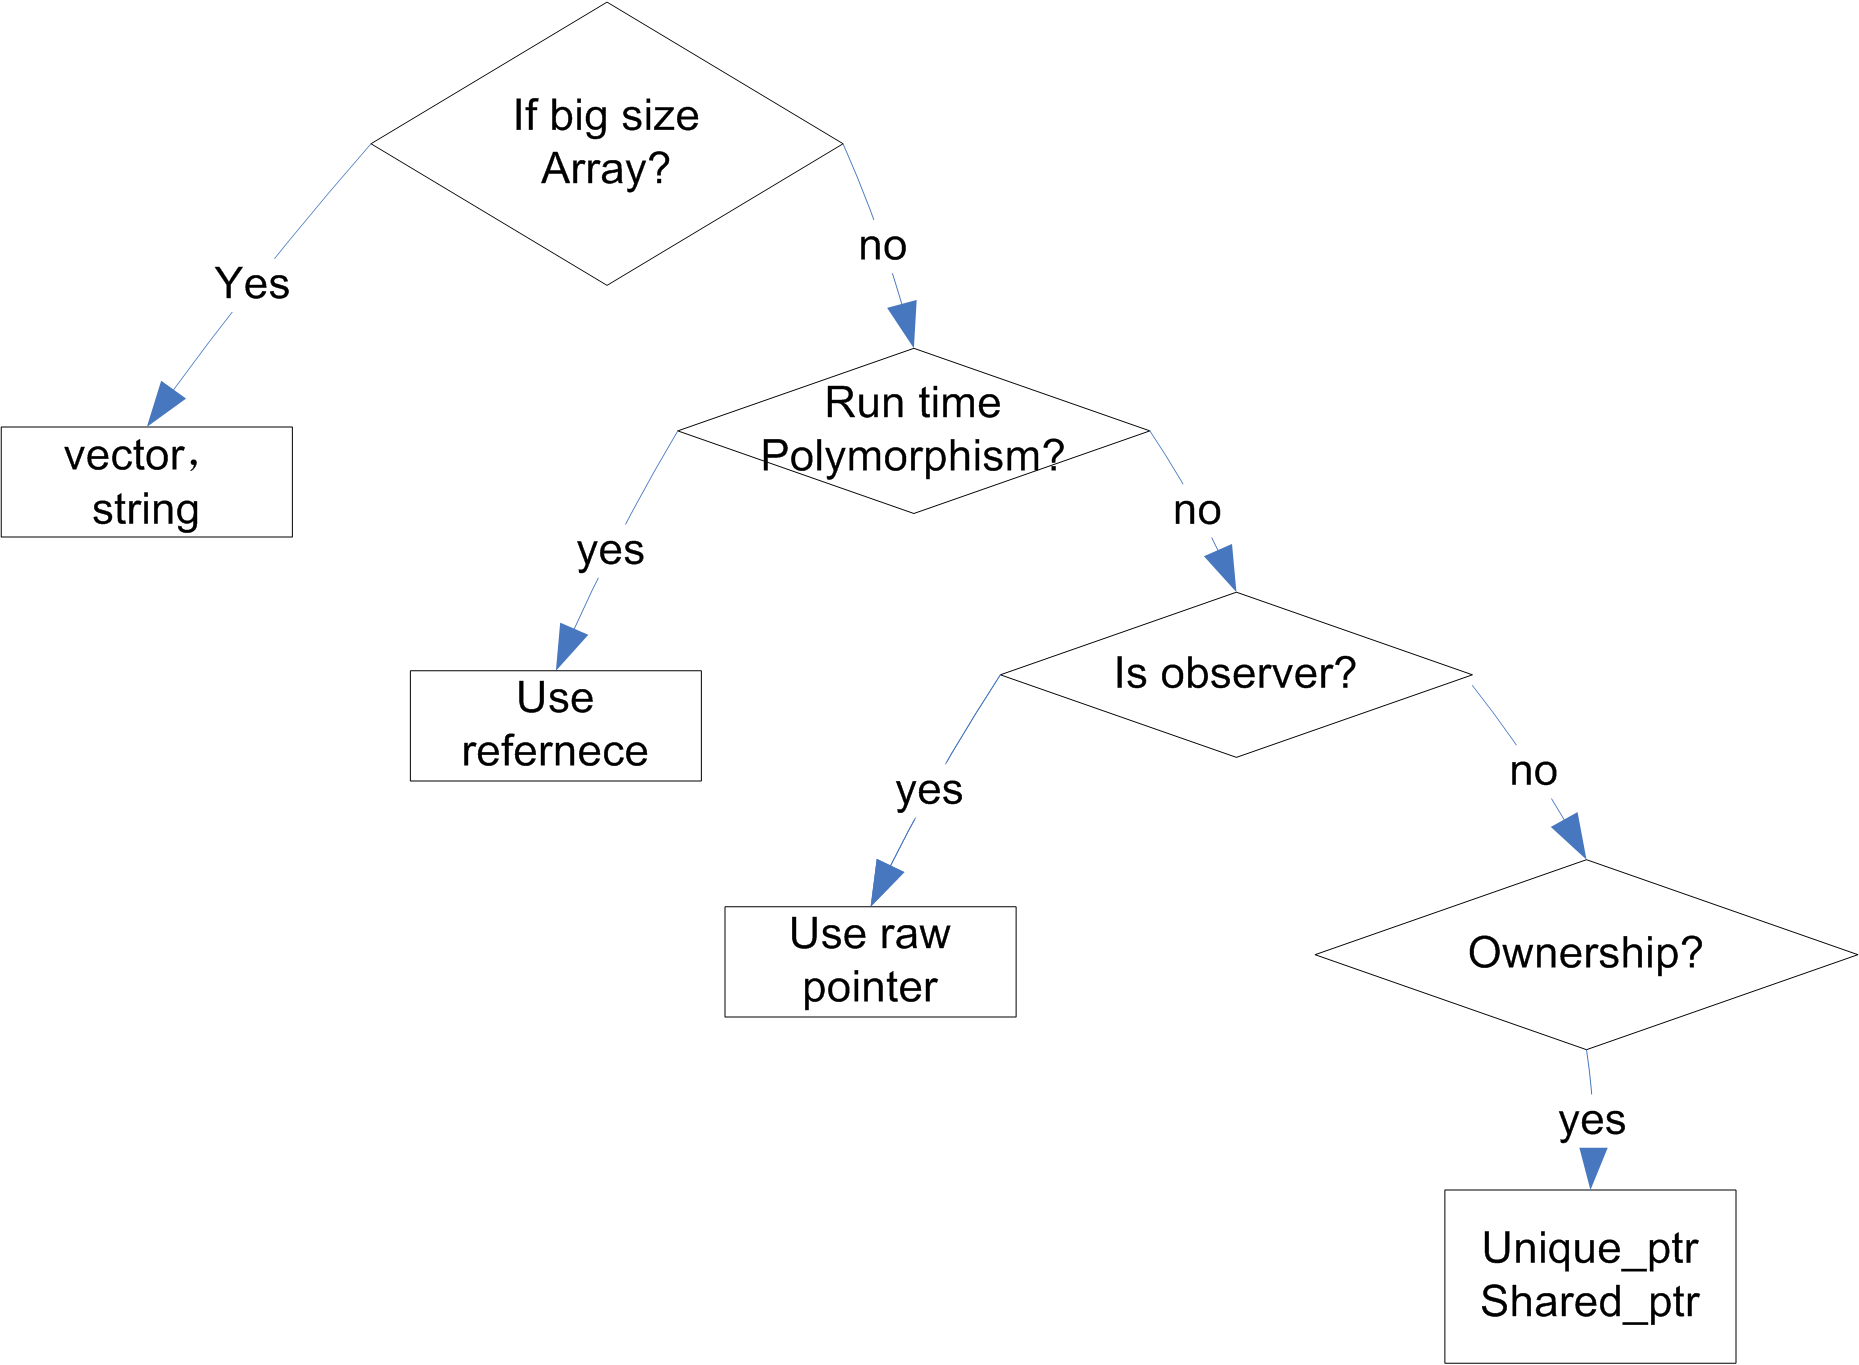
\includegraphics[width=0.75\linewidth]{pics/smartPointer.png}
	\caption{When to use smart pointer?}
	\label{fig:smartpointer}
\end{figure}
\end{itemize}

\chapter{lvalue reference and rvalue reference}
\section{lvalue, rvalue and lvalue reference}
\subsection{Value categories}

\begin{itemize}

	\item Each C++ expression (an operator with its operands, a literal, a variable name, etc.) is characterized by two independent properties: \textbf{type and value category}. Each expression is certain kind of type, such as \texttt{int} type, reference type or rvalue reference type. Each expression belongs to exactly one of the three primary value categories: \textbf{lvalue, prvalue, and xvalue;} We will introduce xvalue later. 
			
    \item Value categories determines two important-but-separate properties about an expression. One property is whether the expression has identity. An expression has identity if it refers to an object that has a variable name. The variable name may not be involved in the expression, but the object can still have one. The other property is whether it is legal to implicitly move from the expression's value. Or more specifically, whether the expression, when used as a function parameter, will bind to r-value parameter types or not.

	\item lvalue is not defined "can be put on the left side of =". Because \texttt{const int a} is also a lvalue, and you can't put a on the left side of = . It has three characteristics:
\begin{enumerate}
	\item\textbf{lvalue has Identity}, (can get address by \& operator),
	\item \textbf{lvalue can be persist beyond the expression. }
	\item \textbf{lvalue can be copied, can't be moved,} because you need to keep original one intact.
\end{enumerate}

	\item On the contrary, prvalue has no \textbf{identity}, and will not \textbf{persist} beyond expression and should be moved for certain resource type object efficiently.

	\item Why rvalue doesn't persist? because rvalues in C++ stored differently. It's freedom for the compiler to improve performances of your code. A more concrete way to understand this is to remember that a value can be stored in a register of your CPU and never actually be in your memory which more or less means that the value has no address. I won't bet everything I have on it but this is probably one of the main reasons why "we cannot get an address of an rvalue". In a more general way since an rvalue is semantically temporary it is more likely to be put in temporary places or optimized in a way where it cannot easily be mapped to an address and even if it can that would be counter productive in terms of performance.

\item lvalue examples. string literal is an lvalue. \textbf{Any function which returns lvalue reference is lvalue.}
\begin{lstlisting}
"abc" //lvalue, different with 42.
int a{}; //name varabile 
int& foo();
foo(); //return reference.
++a; //prefix operator
*(p+1); //dereference of pointer
f.a // if f is lvalue.
\end{lstlisting}
	
	\item rvalue examples: \textbf{Any function which returns value is rvalue.}
\begin{lstlisting}
42    // literal
int foo(); 
foo(); //function call return value
a+b;   //result of arithmetic
&a //address 
satic_cast<doulbe> a //casting
a++; //postfix operator
double{}; //tempory variable
\end{lstlisting}

	\item Remember that any expression that evaluates to an lvalue reference (e.g., a function call, an overloaded assignment operator, etc.) is \textbf{an lvalue}. Any expression that \textbf{returns an object by value is an rvalue}.

\begin{lstlisting}[frame=single, language=c++, mathescape=true]
string& lvalue_fun();
lvalue_fun(); 
lvalue_fun() = "hello"; //OK
&lvalue_fun();          //OK
	
string pvalue_fun();
pvalue_fun(); 
pvalue_fun() = "hello"; //ERROR
&pvalue_fun();          //ERROR
\end{lstlisting}

\begin{description}
	\item[Line 2 to 4:] After you call this fun, lvalue still exist. you can modify because it persist. you can get address because it has identity. call copy constructor, can't move
	
	\item[Line 6 to 9:]  After call this fun, value disappear. NOT modify because it doesn't persist. NOT get address because it no identity. call move constructor, can move
\end{description}
\end{itemize}

\subsection{lvalue reference basic}

\begin{itemize}
    \item \textbf{Reference has two characteristics, no null, no change}. In other words, top level of const of reference is default. You can't change it. A reference always refers to the object with which it's initialized firstly. That is why you have to initialize it.
\begin{lstlisting}[numbers = none]
string &rs = s1;
rs = s2; //modified s1's value,rs still refer to s1
\end{lstlisting}

    \item Reference is different with pointer. Reference has no wild pointer problem. So a reference doesn't need to be test if it's null reference. If you have a reference to a local variable inside a function, when the function finishes, it still have dangling reference problem. 
\begin{lstlisting}[numbers=none]
if(pointer) // don't need for a reference.
cout<< *pointer <<endl;
\end{lstlisting}

    \item you can have reference to pointer, but pointer to reference is illegal. In grammar level, reference to reference has different means, it's called rvalue reference. This doesn't exist. As stated earlier, a reference is merely an alias to another object. You can't "point" to a reference, because it isn't an object in itself but merely another name for a real object. 
\begin{lstlisting}[numbers=none]
int *p;
int *& rp = p; // reference to pointer is OK
int &* pr  //pointer to reference is ERROR
int && rv //that is rvalue reference.
\end{lstlisting}


\item non-const reference can't refer to const object.
\begin{lstlisting}[numbers=none]
const int i = 12;
int& j = i; //ERROR
\end{lstlisting}

\item A \texttt{const} object reference passed into a function, if you want to return it , it must be \texttt{const} too. Usually, It has no any practical meanings when you do in this way. 
\begin{lstlisting}[numbers=none]
const int &fun(const int& i){ 
	return i;
}
//or const_cast 
int &fun(const int& i){ 
	return const_cast<int&>(i);
}
\end{lstlisting}

\item  \texttt{const} reference can bound to temporary. Temporary is not lvalue, and only lvalue can bound to reference to \texttt{non-const}.   
\begin{lstlisting}[frame=single, language=c++]
Foo f(){ //case 1:
	return obj;
}
const Foo & rf = f();

class Foo(int i); // case 2:
f(const Foo & crf); //function declaration

f(1);
\end{lstlisting}
\begin{description}
	\item[Line 4:] Only \texttt{const} reference can bound to temporary and prolong temporary variable life. Only stack-base \texttt{const} reference can work in this way. If a \texttt{const} reference is class member, it can't work. 
	
	\item[Line 9:] temp obj build by constructor, if you skip const in line 7 function declartion, compiler will report error.
\end{description}

	\item \texttt{const} reference bound to rvalue is used in copy constructor widely. But in C++11, For a class with a lot allocated resource, please use move copy ctor which explained in the next section:

\begin{lstlisting}[]
class Foo{
	Foo(const Foo & foo);
}

Foo f3 = f1+f2;
\end{lstlisting}
\begin{description}
	\item[Line 5:] because a temp Foo is produced first from \texttt{f1+f2}. Without \texttt{const} in copy constructor, compiler will bark.
\end{description}

\end{itemize}

\subsection{lvalue reference overload}
\begin{itemize}
		\item Reference type will not decide overload resolution.
\begin{lstlisting}[numbers=none]
void foo(int x)  { std::cout << "foo(int)"   << std::endl; }
void foo(int& x) { std::cout << "foo(int &)" << std::endl; }

int i = 42;
int &j = i;
foo(i);  //ambiguous call
foo(j);  //ambiguous all
\end{lstlisting}
\begin{description}
	\item[Source code:] Even \texttt{j} is reference type(\texttt{int \&}), it still trigger ambiguous call.
\end{description}

		\item \texttt{const} will not help to distinguish value and reference type.
\begin{lstlisting}[numbers=none]
void foo(int x)  { std::cout << "foo(int)"   << std::endl; }
void foo(const int& x) { std::cout << "foo(cons int &)" << std::endl; }

int i = 42;
const int &j = i;
foo(i); // ambigous call
\end{lstlisting}

	\item \texttt{const} will help to distinguish between reference type.
\begin{lstlisting}[numbers=none]
void foo(int &x)  { std::cout << "foo(int&)"   << std::endl; }
void foo(const int& x) { std::cout << "foo(cons int &)" << std::endl; }
	
int i = 42;
const int &j = i;
foo(j); // call const version
\end{lstlisting}


		\item lvalue reference can only bound to lvalue, so we can use value category, help us to pick up the right function.
\begin{lstlisting}[numbers=none]
void foo(int x)  { std::cout << "foo(int)"   << std::endl; }
void foo(int& x) { std::cout << "foo(int &)" << std::endl; }

foo(2);	 //call foo(int x),2 is prvalue, so int& can't matches
\end{lstlisting}

\begin{lstlisting}[numbers=none]
void foo(int x)  { std::cout << "foo(int)"   << std::endl; }
void foo(int& x) { std::cout << "foo(int &)" << std::endl; }
void foo(const int& x) { std::cout << "foo(cons int &)" << std::endl; }
	
foo(2);	 //ambious, 2 is prvalue, so const int & and int both match
\end{lstlisting}

\item summary:
\begin{enumerate}
	\item Given lvalue, reference type and value type produce ambiguous call.
	\item Given lvalue, constness can't help distinguish reference type and value type.
	\item Given const lvalue, constness help to distinguish const reference type and lvalue reference type.
	\item both value and const lvalue reference can match rvalue, but lvalue reference can not. 
\end{enumerate}
\begin{center}
	\begin{tabular}{|c|c|c|c|}
		\hline
		& value & lvalue reference  & const lvalue reference  \\
		\hline
		lvalue & OK &  OK & OK  \\
		\hline
		rvalue & OK & Not & OK   \\
		\hline
	\end{tabular}
\end{center}

\end{itemize}

\section{rvalue reference and move semantic}
\subsection{Rvalue reference}
\begin{itemize}
	
	\item rvalues denote temporaries or objects that want to look like a temporary. What is so particular about temporaries, is the fact that they will be used in a very limited way: their value will be read once, and they will be destroyed. This is a very useful observation in implementing "move semantics." 
	
	\item How to understand move semantics? Move is not really move a big chunk of data, It just move index of data. just like you move file in the hard disk. 
	
	
	\item Typically, if your class allocate a lot of allocated resource (new, or manually manage some system resources).  You should implement copy constructor to avoid shallow copy. 
\begin{lstlisting}[numbers=none]
Foo::Foo(const Foo & rhs){
	while(ptr++;)
	  ptr[i] = foo.ptr[i]  //expensive copy
}
\end{lstlisting}

	\item The problem is for some rvalue, we also need to perform expensive copy. 
\begin{lstlisting}[frame=single, language=c++]
Foo foo1 = foo2;
Foo foo1 = foo2+foo3; //rvalue
Foo foo1 = getFoo(); //rvalue
\end{lstlisting}

\begin{description}
	\item[Line 2-3:] right side produce rvalue, copy from temporary variable(rvalue) is waste, because temporary variable will disappear and we don't need to keep intact. 
\end{description}

	\item \textbf{We usually use type as overload resolution method. For reference type, we can use value category as overload resolution method. For example, before C++ 11, rvalue only match const lvalue reference, it will not match lvalue reference}. But const lvalue reference has problem, const reference can bind both lvalue and rvalue, so we can't distinguish when to move, when to copy, that is the problem of efficiency. At the same time, we can't change it. For rvalue, sometimes, we don't want to expensive copy it, but cheap move it. That is why we need a kind of reference type. Once we have such new reference type,  allow a function to branch at compile time (via overload resolution) on the condition "Am I being called on an lvalue or a rvalue?" \textbf{ we have two requirements here for the new reference type: it only binds to rvalue, and we can change it}. In below code, What should ???? be? \textbf{Although \texttt{foo2} and \texttt{foo2+foo3} have the same type, but have different value categories(One is lvalue and the other is rvalue)}. That is why we \textbf{invent rvalue reference in C++ 11}. Which can only bind to rvalue. 

\begin{lstlisting}[frame=single, language=c++]
Foo::Foo(const Foo & rhs){ //copy constructor
	while(ptr++;)
	    ptr[i] = rhs.ptr[i]  //expensive copy
}	

Foo::Foo(???? rhs){  //move constructor
	ptr = rhs.ptr;  //efficient move(steal)
	rhs.ptr = nullptr;
}	
	
Foo foo1 = foo2;  //use the first copy constructor
Foo foo1 = foo2+foo3;  //for right value, use move constructor
Foo foo1 = getFoo();  //for right value, use move constructor
\end{lstlisting}

\begin{center}
		\begin{tabular}{|c|c|}
			\tophline 
			type & which value category can bind \\ 
			\tophline 
			lvalue reference & lvalue(non-const)  \\ 
			\tophline 
			rvalue reference &  rvalue(non-const)\\ 
			\tophline 
			const lvalue reference & lvalue or rvalue(const or non-const)  \bottomhline 
		\end{tabular} 
\end{center}

\end{itemize}

\subsection{ rvalue reference and move constructor}

\subsubsection{rvalue reference basic}
\begin{itemize}
	\item If \texttt{X} is any type, then \texttt{X\&\&} is called an rvalue reference to \texttt{X}. For better distinction, the ordinary reference \texttt{X\&} is now also called an lvalue reference. Rvalue references will implicitly bind to rvalues and to temporaries that are the result of an implicit conversion. i.e. Below is well formed because float is implicitly convertible to int; the reference would be to a temporary that is the result of the conversion.
\begin{lstlisting}
float f = 0f; 
int&& i = f; 
\end{lstlisting}
	
	\item Rvalue references can be used to extend the lifetimes of temporary objects (note, lvalue references to const can extend the lifetimes of temporary objects too, but they are not modifiable through them):
	
\begin{lstlisting}[frame=single, language=c++, mathescape=true]
std::string s1 = "Test";
std::string&& r1 = s1; //ERROR rvalue reference can't bind to lvalue.
		
const std::string& r2 = s1 + s1;//lvalue reference to const extends lifetime. 
r2+="test" //Error  can't modify through reference to const.
		
std::string&& r3 = s1 + s1; //rvalue reference extends lifetime
r3 += "Test"; //can modify through reference to non-const.                   
\end{lstlisting}
	

	\item The most important thing to remember is that value categories are a taxonomy of expressions. They are not categories of objects or variables or types. Getting this wrong is an immediate source of problems. 
\begin{lstlisting}[frame=single, language=c++, mathescape=true]
void foo(int& );  // #1
void foo(int&& ); // #2

int&& r = 42;
foo(r); // will call #1, because r is lvalue, although type is rvalue reference.
\end{lstlisting} 

\item \textbf{Things that are declared as rvalue reference can be lvalues or rvalues. The distinguishing criterion is: if it has a name, then it is an lvalue. Otherwise, it is an rvalue.} Understand this word is very important, In the previous code, r has name, so it is lvalue, When we use \texttt{std::move}, it "erase" the name by a function call, so unname rvalue reference is rvalue.
	
\end{itemize}

\subsubsection{move constructor implementation and usage}
\begin{itemize}
	\item An example code for move constructor and move assignment.	
\begin{lstlisting}[numbers=none]
Foo::Foo(const Foo & rhs){
	while(ptr++;)
	  ptr[i] = rhs.ptr[i]  //expensive copy
}
Foo::Foo(Foo && rhs){ //no const here
	ptr = rhs.ptr;  //efficient move(steal)
	rhs.ptr = nullptr;
}
Foo& Foo::operator=(Foo&& rhs){
	delete[] ptr;
	ptr = rhs.ptr;  //efficient move(steal)
	rhs.ptr = nullptr;
	return *this;
}
\end{lstlisting}
	

	
	\begin{enumerate}
		\item Move constructor will not move resource automatically, you need to coding it by your self. You can't move in normal constructor. because, It must keep origin obj intact.  You can steal when \texttt{Foo(f1+f2)}, but when you used \texttt{Foo(f1)}.  It will destroy \texttt{f1}. Without  move constructor, normal copy constructor will treat \texttt{Foo f = f1+f2} and \texttt{Foo f = f1} the same way.
		
		\item With move copy constructor, normal copy constructor deal with \texttt{Foo f = f1}, and move copy constructor deal with \texttt{Foo f = f1+f2}, for \texttt{f1+f2}, you can steal resource, because nobody need to use \texttt{f1+f2} later any more. \item \textbf{In move constructor, always set rhs.ptr = nullptr;} \item No const qualifier in move constructor and move assignment
		
	\end{enumerate}
	
%	\item In below examples, Foo obj1=obj2+obj3. if you don't have move constructor, In operator + function, a temp obj is produced,  and when operator+ function return, another temp obj temp2 is produced .  Then in the end, objtemp2 is passed to ctor,  So, ctor is called three times. and copy content is also called three times.
%	
%\begin{lstlisting}[numbers=none]
%	Foo Foo::operator+( const Foo & f) const {
%			Foo temp = Foo(n+f.n);
%			//copy happen here.
%			return temp;
%		}
%		
%		Foo obj1=obj2+obj3  
%		// three constructor called without move ctor
%	\end{lstlisting}
%	
%	\item If you have move constructor. In operator + function, a temp objtemp1 is produced,  When return objtemp1, It will not produce objtemp2. (because objtemp1 is rvalue.) then objtemp1 is passed to move ctor. In side move ctor, the resource address has been move to new obj1.  Just one temp objtemp1 and one actual copy happen. ( just new pointer = old pointer; and old pointer = NULL).


\item Don't declare objects \texttt{const} if you want to be able to move from them. Move requests on \texttt{const} objects are silently transformed into copy operations.

\end{itemize}

\section{xvalue}
\begin{itemize}
	\item In this section, there are four important points
	\begin{enumerate}
		\item \texttt{std::move} and why do we need a new value type--xvalue?
		\item Academic definition of xvalue.
		\item Give some practical expressions which are xvalue.
		\item Relationship between xvalue and rvalue reference.
	\end{enumerate}
\end{itemize}

\subsection{std::move function}

\begin{itemize}
	\item C++11 allows you to use move semantics not just on rvalues, but, at your discretion, on lvalues as well. An good example is swap function, here if you can move lvalue, the efficiency will be better. 
	
\begin{lstlisting}[numbers=none]
template<class T> 
void swap(T& a, T& b) { 
	T tmp(std::move(a));
	a = std::move(b);  //std::move must return rvalue.
	b = std::move(tmp);
} 
\end{lstlisting}
	
	\item By now, \texttt{std::move} must return rvalue, How?
	\begin{enumerate}
		\item If \texttt{std::move} return  value? \texttt{std::move(b)} is rvalue, but not good. Because it means that we have to copy once inside \texttt{std::move} but in input a value, then return value, you must copy inside this function.
		
		\item If \texttt{std::move} return  lvalue reference? \texttt{std::move(b)} is lvalue. 
		
		\item If \texttt{std::move} return  rvalue reference? \texttt{std::move(b)} is rvalue. Good! 
	\end{enumerate} 

    \item for this kind of rvalue reference, we can put it on the left side of assignment, so it's not prvalue. At the same time, you can move it, so it's not lvalue.  \textbf{In this way, we have to introduced a new value type--xvalue.}    
\begin{lstlisting}[frame=single, language=c++, mathescape=true]
string str = "hello"
std::move(str)[0] = 'z';  //can modify
string str1 = std::move(str) //can move
\end{lstlisting}
\begin{description}
	\item[Line 2-3:] print "zello" here. Because std::move() return a xvalue, it can persist and move.
\end{description}
	
    \item  \texttt{std::move} not only doesn't actually move anything, it doesn't even guarantee that the object it's casting will be eligible to be moved. The only thing you know for sure about the result of applying \texttt{std::move} to an object is that it return a xvalue.

\begin{lstlisting}[frame=single, language=c++]
explicit Annotation(const std::string text)
: value(std::move(text)) 
\end{lstlisting}
\begin{description}
	\item[Line 1:] That is constructor, we want to "move" text into value; this code doesn't do what it seems to, because text is const
\end{description}
	
	\item Summary:
	\begin{enumerate}
		\item We have rvalue reference to bind temporary value to move it.
		\item We want to move a lvalue, such as swap, so we have \texttt{std::move()} function.
		\item \texttt{std::move()} return neither lvalue nor prvalue, so we have to define a new type of value--xvalue.
	\end{enumerate}
	
\begin{center}	
		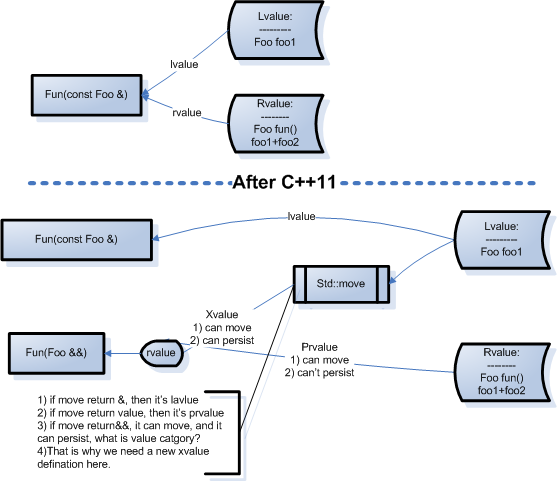
\includegraphics[width=0.7\linewidth]{pics/xvalue.png}
		\label{fig:xvalue}
    \end{center}
\end{itemize}


\subsection{new value category}

\begin{itemize}
	\item xvalue definition: a function call or an overloaded operator expression, whose return type is rvalue reference to object. That is to say, an xvalue is the result of certain kinds of expressions involving rvalue references. \textbf{The result of calling a function whose return type is an rvalue reference is an xvalue.} fun return lvalue reference is lvalue, fun return value is pvalue, and fun return rvalue reference is xvalue.
	
	\item In definition,  xvalue is just value with identity and can be movable. \textbf{In real life, it's  return value of std::move() or static\_cast<A\&\&>}. A better introduction can be seen: " C++11 Tutorial: Explaining the Ever-Elusive Lvalues and Rvalues"
	
	
	\item First, we can use \textbf{persist and identity} to classify value into lvalue and rvalue, then c++11 introduce \textbf{std::move}. The return value of \texttt{std::move} is unnamed rvalue reference. this unnamed rvalue reference can persist and move at the same time.  So we divide lvalue into lvalue and xvalue and give them new name.  lvalue+xvalue = glvalue(persist)  and xvalue + prvalue = rvalue(move).
	
	\item \textbf{Any value must be one of three value categories: lvalue, xvalue, or prvalue.} These three categories are complementary.  \textbf{lvalue pay attention to  identity and persist, rvalue = (xvalue + prvalue) shout "I can be moved" loudly.  So we call \&\& rvalue reference, don't call it xvalue reference. }
	
	\begin{figure}[h]
		\centering
		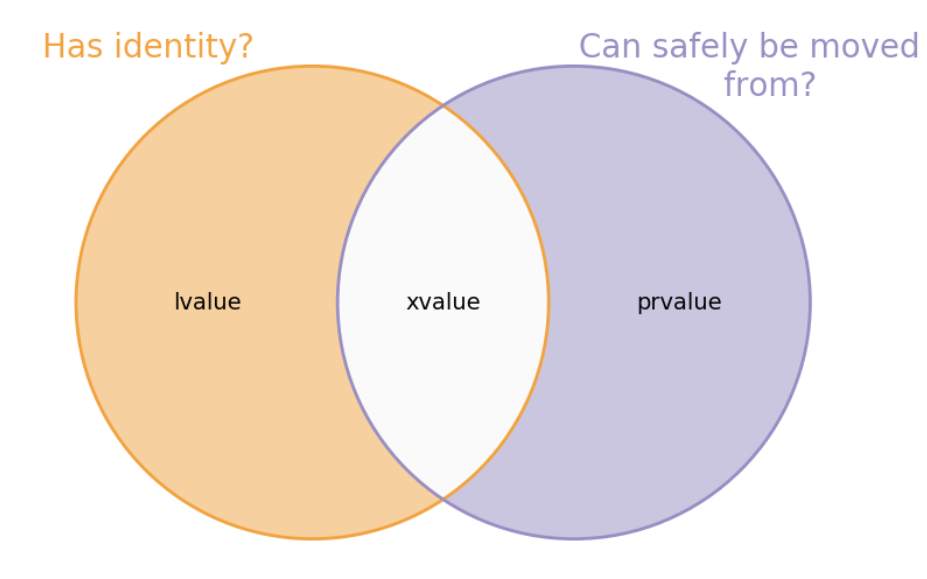
\includegraphics[width=0.4\linewidth]{pics/xvalue1.png}
		\caption{lvalue, rvalue and xvalue.}
		\label{fig:xvalue1}
	\end{figure}
	
	
	\item Distinguishing these three value categories is very important when you try to understand decltype deducting rule. I will introduce in "Generic programming" chapter.
	
	\item Summary table: 
	\begin{center}
		\begin{tabular}{|c|c|c|}
			\tophline
			& persist(Identity) & move \\
			\tophline
			lvalue & Yes & No \\
			\tophline
			pvalue & No & Yes \\
			\tophline
			xvalue & Yes & Yes \bottomhline
		\end{tabular}
	\end{center}
	



\item Using forward reference to judge if a var is lvalue.
\begin{lstlisting}[frame=single, language=c++]
template <typename T>
constexpr bool is_lvalue(T&&) {
	return std::is_lvalue_reference<T>{};
}

std::string a("Hello");
is_lvalue(std::string()); // false
is_lvalue(a); // true  
\end{lstlisting}

\begin{description}
    \item[Line 8:] in the case you pass a \texttt{std::string} lvalue, then T will deduce to \texttt{std::string\&} or \texttt{const std::string\&}, for rvalues it will deduce to \texttt{std::string}.
\end{description}

\item \textbf{How to determine programmatic if an expression is rvalue or lvalue}
\begin{lstlisting}[numbers=none]
if (std::is_lvalue_reference<decltype(var)>::value) {
	// var was initialised with an lvalue expression
} else if (std::is_rvalue_reference<decltype(var)>::value) {
	// var was initialised with an rvalue expression
}

string&& xvalue_fun();
std::is_rvalue_reference<decltype(xvalue_fun())>::value
//return true
\end{lstlisting}

\end{itemize}

\subsection{xvalue and rvalue reference}

\begin{itemize}

    \item An example of xvalue.
\begin{lstlisting}
string&& xvalue_fun();

xvalue_fun(); //After you call this fun, value still exist. 
xvalue_fun() = "hello"// You can modify because it persist.
&xvalue_fun(); //You can get address because it has identity.
string a = xvalue_fun();// call move constructor, can move.
\end{lstlisting}
	
	\item More xvalue examples.
\begin{lstlisting}[frame=single, language=c++, mathescape=true]
struct A {
	int m;
};
	
A&& operator+(A, A); // a+a is xvalue
A&& f();  //f() is xvalue
f().m // f().m is also xvluae
A a;
A&& ar = static_cast<A&&>(a); static_cast<A&&>(a) is xvalue, but ar is lvalue
\end{lstlisting}
	
	\item After C++11, we added two new xvalues.
	\begin{enumerate}
		\item \texttt{a[n]}, the built-in subscript expression, where one operand is an array rvalue;
		\item \texttt{a.m}, the member of object expression, where a is an rvalue and m is a non-static data member of non-reference
	\end{enumerate}

	\item \textbf{xvalue is defined based on rvalue reference. But you can't think that a rvalue reference is a xvalue. }  \textbf{A named rvalue reference is lvalue, and unnamed rvalue reference is xvalue};
	
\begin{lstlisting}[frame=single, language=c++,mathescape=true]
void foo(int&& t) {
//t is initialized with an rvalue expression, but is actually an lvalue expression itself
}
	
std::string a;   //a, b, c are all lvalue.
std::string& b;
std::string&& c;
\end{lstlisting}
	

	\item Why is there such confusion? Here are the circumstances under which it is safe to move something:\\
	1) When it's a temporary or sub-object thereof. (prvalue) \\
	2) When the user has explicitly said to move it.
\begin{lstlisting}[frame=single, language=c++]
SomeType &&Func() { ... }
	
SomeType &&val = Func();
SomeType otherVal{val}; // Do you really want to move 
	....
cout<<val; 
\end{lstlisting}
\begin{description}
	\item[Line 6:] what happen if you have forget you have move? it will crash the problem. so standard said that val is lvalue. because it's a named rvalue reference.
\end{description}
	
    \item Another deep trap happen when you implement move constructor in derived class
\begin{lstlisting}[numbers=none]
Derived(Derived&& rhs):Base(rhs)//wrong: rhs is an lvalue
{
	// Derived-specific stuff
}
	
Derived(Derived&& rhs) : Base(std::move(rhs)){
	// good, calls Base(Base&& rhs)
}
\end{lstlisting}
	
\end{itemize}



\section{Universal(forwarding) reference }
\subsection{definition}

\begin{itemize}
\item You need to know two prerequisites before you understand forwarding reference:

\begin{enumerate}
	\item In pre-11 C++, it was not allowed to take a reference to a reference: something like \texttt{A\&\&} would cause a compile error. C++11, by contrast, introduces the following reference collapsing rules1:
	
\begin{lstlisting}[numbers=none]
A& & becomes A&
A& && becomes A&
A&& & becomes A&
A&& && becomes A&&
\end{lstlisting}
	
	\item forwarding reference type deduction rules: For lvalue and rvalue, we use the different rule to deduct type.
\end{enumerate}

    \item \textbf{Universal reference has been renamed as forwarding reference}. It's more descriptive name, It tell you universal reference should always been used with forwarding.

    \item  Universal references arise in two contexts. The most common is function template parameters. The second context is auto\&\&\textbf{1)must be constrained T\&\& form, 2) type deduction happen.} If the form of the type declaration isn't precisely type\&\&, or if type deduction does not occur, type\&\& denotes an rvalue reference.
\begin{lstlisting}
auto&& var2 = var1; // universal reference

template<typename T>
void f(T&& param); // universal  reference

template<class T, class Allocator = allocator<T>>
class vector {
	template <class... Args>
	void emplace_back(Args&&... args); //args is forwarding reference. 
};

//------------below are not universal reference----
template<typename T>
void f(std::vector<T>&& param); // rvalue reference

template<typename T>
void f(const T&& param); // with const

template<class T, class Allocator = allocator<T>>
class vector { 
public:
	void push_back(T&& x); //no type deduction
};
\end{lstlisting}
\begin{description}
	\item[Line 14:] form is quite constrained. It must be precisely \texttt{"T\&\&"}.
\end{description}


\end{itemize}

\subsection{pros and cons of forwarding reference}
\begin{itemize}

\item It can provide the unify interface, and it supports variadic number. That is \texttt{make\_unique} and \texttt{make\_shared} and emplace-kind function possible.

\item If you have a template class or template fun, universal reference is your only choice. An example can be seen in the last chapter, "decltype deduction" section.

\item For overload method, more source code to write and maintain (two functions instead of a single template). For overload method, it can be less efficient. For example, consider this use of setName: w.setName("Adela Novak"); With the version of setName taking a universal reference, the string literal "Adela Novak" would be passed to setName, where it would be conveyed to the assignment operator for the std::string inside w. w's name data member would thus be assigned directly from the string literal; no temporary std::string objects would arise. With the overloaded versions of setName, however, a temporary std::string object would be created for setName's parameter to bind to, and this temporary std::string would then be moved into w's data member.

\begin{lstlisting}[numbers=none]
class Widget {
public:
	template<typename T>
	void setName(T&& newName) // newName is universal reference
	{ name = std::forward<T>(newName); }
...
	string name;    
};
\end{lstlisting}

    \item overload has the poor scalability of the design. Widget::setName takes only one parameter, so only two overloads are necessary, but for functions taking more parameters, each of which could be an lvalue or an rvalue, the number of overloads grows geometrically: n parameters necessitates 2n overloads. Such as \texttt{make\_shared} function, It's also support variadic parameter

\begin{lstlisting}[numbers=none]
template<class T, class... Args> 
shared_ptr<T> make_shared(Args&&... args); 

template<class T, class... Args> 
unique_ptr<T> make_unique(Args&&... args); 
\end{lstlisting}

    \item You can use universal reference,  but inside, you have to use forward function, and implementation is a little difficult.  Detail can be seen "effective modern c++ item 41". As a template, implementation must typically be in a header file. It may yield several functions in object code, because it not only instantiates differently for lvalues and rvalues, it also instantiates differently for std::string and types that are convertible to std::string (see "effective modern C++ item 25"). 

    \item There are argument types that can't be passed by universal reference (see Item 30), and if clients pass improper argument types, compiler error messages can be intimidating (see "effective modern C++ item 27").

\begin{lstlisting}[numbers=none]
template<typename T> // reference
fun(T&& value){
	vector<Foo> vect;
	vect.push_back(std::forward<T>(value)); 
}
\end{lstlisting}

    \item Overloading on universal references almost always leads to the universal reference overload being called more frequently than expected.

    \item Perfect-forwarding constructors are especially problematic, because they're typically better matches than copy constructors for non-const lvalues, and they can hijack derived class calls to base class copy and move constructors. detail can be seen in "effective modern c++ item 26"

\end{itemize}

\subsection{Usage of forwarding reference}
\begin{itemize}
\item When to use universal references? universal means that:
\begin{enumerate}
	\item you have to support different type or a lot of parameter. 
	\item You have to use reference, means that need refer a existing one, you refer it because you want to copy it inside of your template function. 
\end{enumerate}

\item There are some points here:
	\begin{enumerate}
		\item \textbf{The first of first, it's only used in a template function.}  \textbf{Inside the function, A copy will happen, if just read or write, use reference or const reference directly}
		
		\item \textbf{When copy, move is cheap, if there is no pointer or contaner, only has POD type value, move is just like copy. You don't need to use universal references.} Most of time, in your universal function, you have a container(string is container too), because move container is much cheaper than copy it.
		
		\item \textbf{For universal reference, you must forward it to constructor, container, object or function. and these four things will take different action toward lvalue and rvlaue.}
		
		\item \textbf{There are more than 2 parameters, and overload function will cause exponential increase.}

		\item I will accept any initializer regardless of whether it is an lvalue or rvalue expression and I will preserve its constness.  This is typically used for forwarding (usually with \texttt{T\&\&}). The reason this works is because a "universal reference", \texttt{auto\&\&} or \texttt{T\&\&}, will bind to anything.  

		\item You might say, well why not just use a const auto\& because that will also bind to anything? The problem with using a const reference is that it's const! You won't be able to later bind it to any non-const references or invoke any member functions that are not marked const.
\begin{lstlisting}[frame=single, language=c++]
auto&& vec=some_expression_that_may_be_rvalue_or_lvalue;
auto i = std::begin(vec);
(*i)++;

auto        // will copy the vector, but we wanted a reference
auto&       // will only bind to modifiable lvalues
const auto& // will bind to anything but make it const, giving us const\_iterator
const auto&& //will bind only to rvalues with const, It's not univerisal reference any more. 
\end{lstlisting} 
	\end{enumerate}

\item There are three function \texttt{emplace\_back}, \texttt{make\_shared} and \texttt{make\_unique}. They use:
	\begin{enumerate}
		\item \textbf{variadic template}, because it need to receive \textbf{any number and any type} parameter.

		\item \textbf{universal reference}, because it's template, and I also want to keep rvalue semantic to improve efficiency. 
		
		\item \textbf{Forward}, because I want to forward parameter to corresponding constructor.Forward only used inside a wrapper, that is to say, to receive universal reference from template wrapper, and forward it to the specific function. The specific function has "COPY" semantic. The more you know these three functions, the better you understand forwarding reference.
	\end{enumerate}
\end{itemize}


\subsection{std::move and std::forward implementation}
\begin{itemize}
	\item Basic implementation of move.
\begin{lstlisting}[numbers=none]
template<typename T> // in namespace std
typename remove_reference<T>::type&&
move(T&& param){
	using ReturnType = typename 
			remove_reference<T>::type&&; 
			
	return static_cast<ReturnType>(param);
}
\end{lstlisting}
	
	\item Basic implementation of forward.
\begin{lstlisting}numbers=none]
template<typename T>
T&& forward(typename remove_reference<T>::type& param){
	return static_cast<T&&>(param);
}
\end{lstlisting}

	\begin{figure}[h]
	\centering
	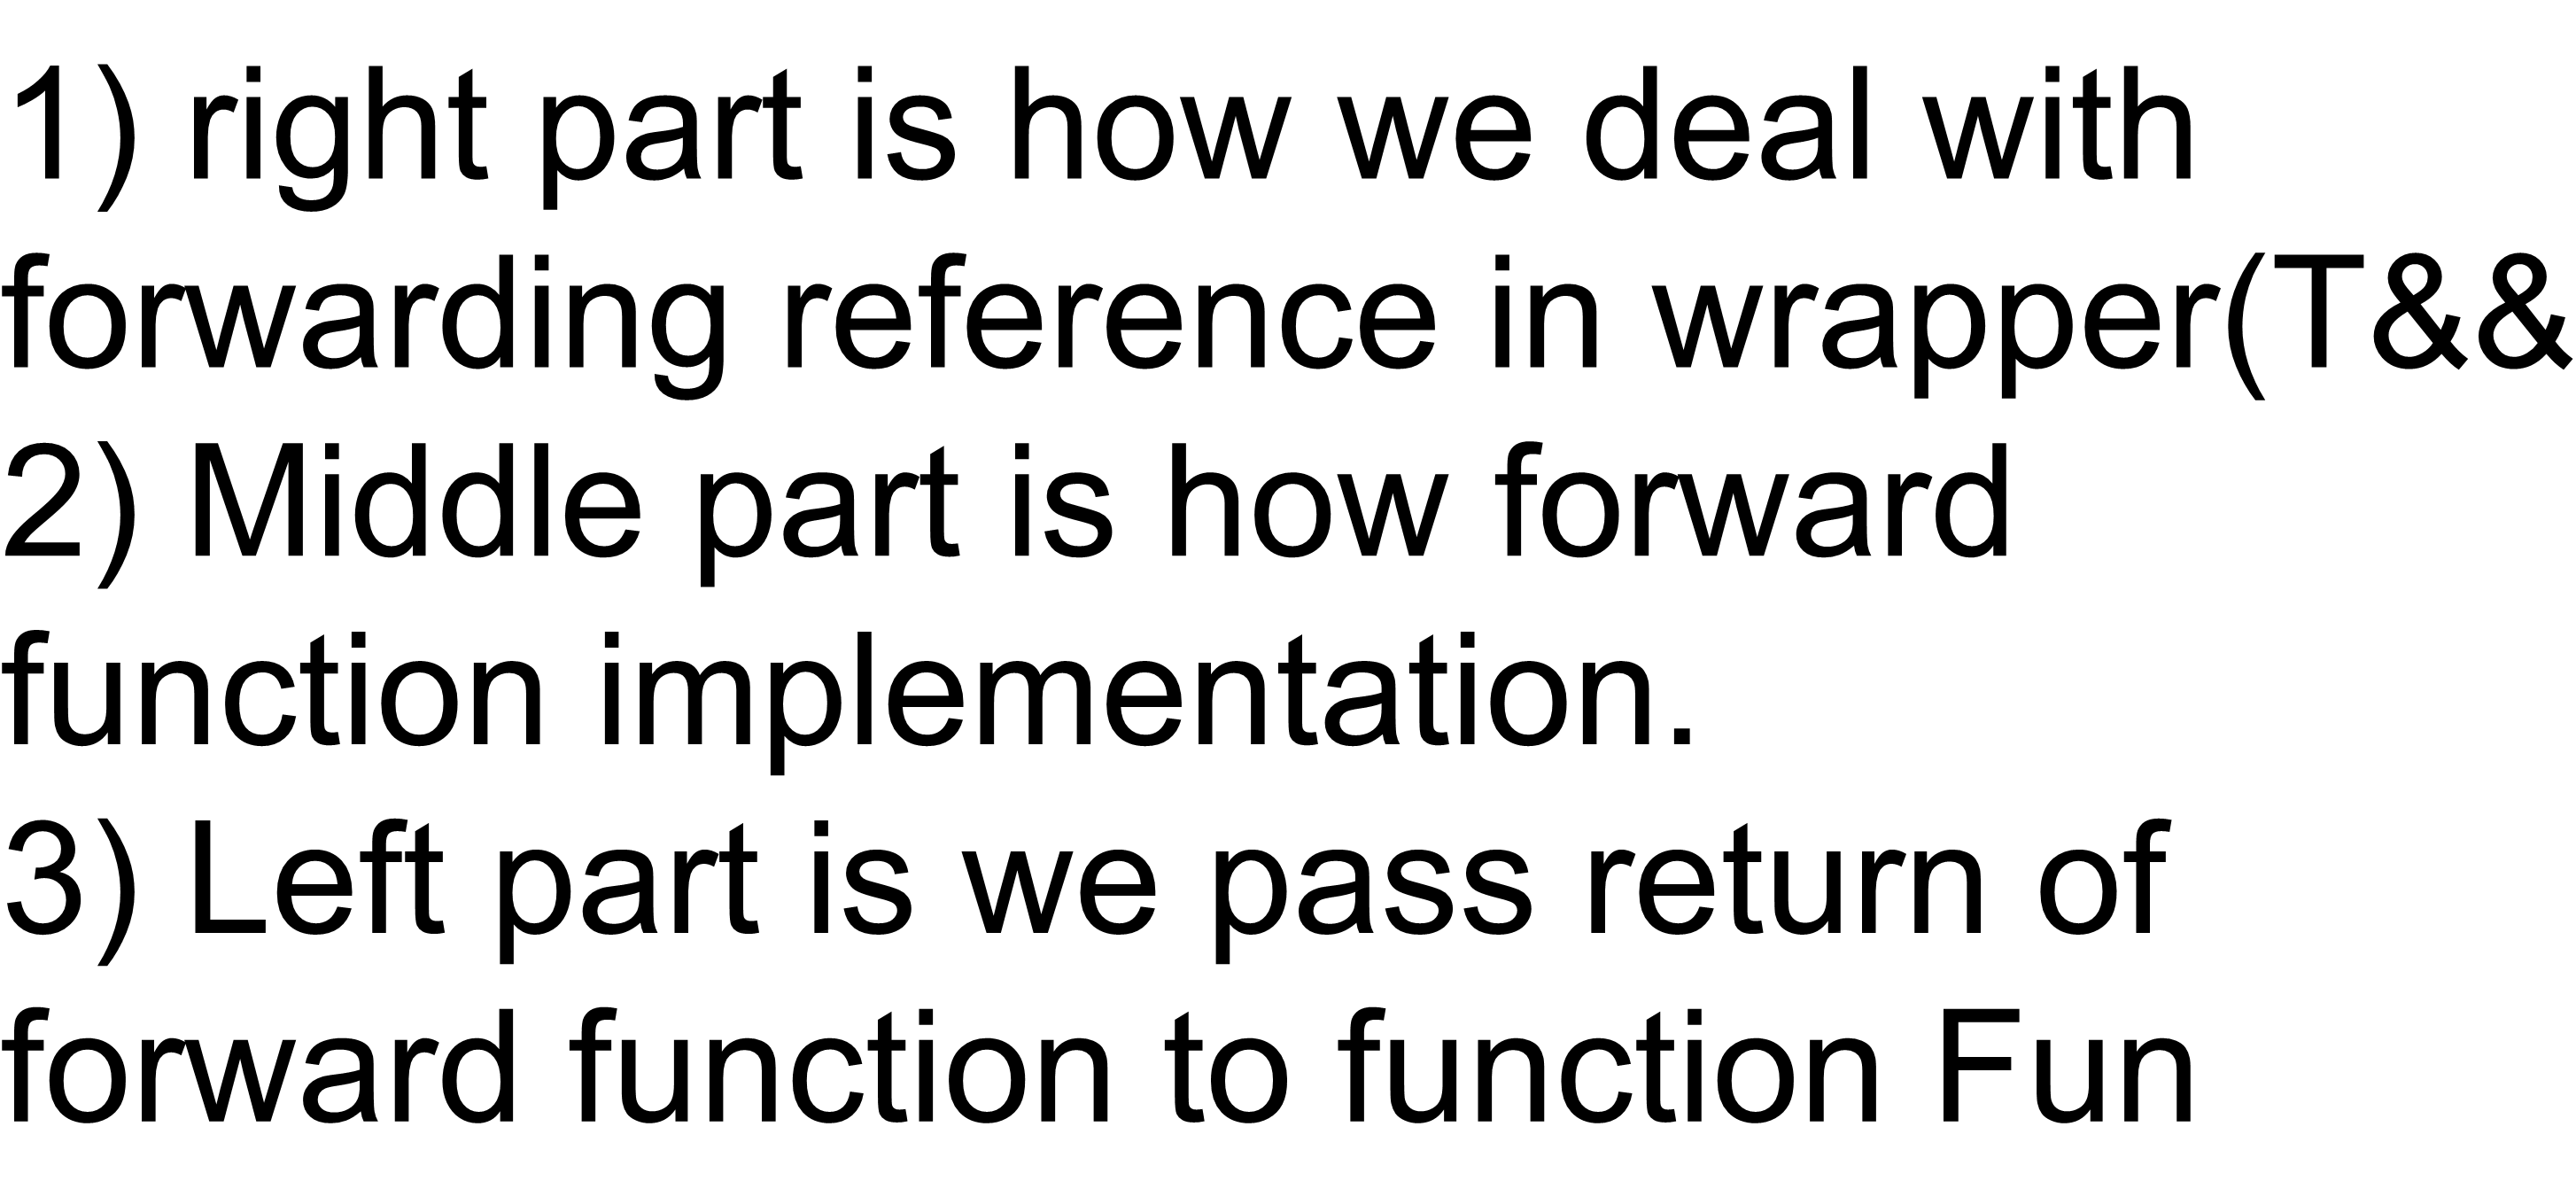
\includegraphics[width=0.85\linewidth]{pics/rvalue_ref.png}
	\caption{move and forward implementation}
	\label{fig:rvalueref}
\end{figure}

    \item A few more explanation about previous implementation:
    \begin{enumerate}
        \item In forward function, why parameter is \texttt{std::remove\_reference\_t<T>\& t}?
\begin{lstlisting}
void fun(int&& r){
	int& r1 = r;  //OK
    forword(int& r1 = r) //Just like this, 
    //int&& r1 = r;  //error: cannot bind 'int' lvalue to 'int\&\&'
    //forword(int && r1 = r) //donsn't work, 
    //That is why we need remove reference on forward function parameter.
    //forward mainly used inside another funciton, outside function parameter has name
    //so they are all lvalue. 
}

int r = 2;
fun(std::move(r));
\end{lstlisting}
\begin{description}
	\item[Line 3:] 
\end{description}

    \item Why std::move use foreard reference as parameter. Just for more generic. We have introduced \texttt{vector<bool>} before, it returns a proxy value and it's rvalue. It's a extreme case, and I admit that. But in generic(template) programming, you will meet it too.
\begin{lstlisting}[]
std::vector<bool> v{true};

std::move(v[0]); // std::move on rvalue, OK
\end{lstlisting}
        \end{enumerate}
    \item There are two important points to help you understand \texttt{std::move} and \texttt{std::forward}. One is forward reference deduct rule, the other is reference collpase rules.
\end{itemize}


\subsection{auto \&\&}

\begin{itemize}
	
	\item \texttt{auto\&\&} isn't used very often, If you don't want to dig too deep, you can skip this section.
	
	
	\item If you then use \textbf{std::forward on your auto\&\& reference} to preserve the fact that it was originally either an lvalue or an rvalue, your code says: Now that I've got your object from either an lvalue or rvalue expression, I want to preserve whichever valueness it originally had so I can use it most efficiently.  For \texttt{auto\&\&}, basic idea just like universal reference, you need to use \texttt{decltype(var)} to get type information when you use forward function on the universal reference. 
\begin{lstlisting}[frame=single, language=c++]
auto&& var = some_expression_that_may_be_rvalue_or_lvalue;
use_it_elsewhere(std::forward<decltype(var)>(var));
\end{lstlisting}
	\begin{description}
		\item[Line 1:] \texttt{var} was initialized with either an lvalue or rvalue, but \texttt{var} itself is an lvalue because named rvalues are lvalues
	\end{description}
	
	\item When to use \texttt{auto\&\&}. I will accept any initializer regardless of whether it is an lvalue or rvalue expression and I will preserve its constness. A good example of \\ "some\_expression\_that\_may\_be\_rvalue\_or\_lvalue;" is illustrated below:
\begin{lstlisting}[frame=single, language=c++]
std::vector<int> global_vec{1, 2, 3, 4};
		
template <typename T>
T get_vector(){
	return global_vec;
}
		
template <typename T>
void foo(){
	auto&& vec = get_vector<T>(); 
	auto i = std::begin(vec);
	(*i)++;
	std::cout << vec[0] << std::endl;
}
		
foo<std::vector<int>>();
std::cout << global_vec[0] << std::endl;
foo<std::vector<int>&>();
std::cout << global_vec[0] << std::endl;
\end{lstlisting}

	\begin{description}
		\item[Line 10:] only \texttt{auto\&\&} work here. \texttt{auto}, \texttt{auto\&} , \texttt{const auto\&}, \texttt{const auto\&\&} all failed.
	\end{description}
	
\end{itemize}



\section{Function interface-parameter}

\subsection{Generic function parameter design}

\begin{itemize}

\item  By now, you imagine that you have a function with parameters, then you have three main operations inside to operate on the parameters: \textbf{1) only read 2) copy from the parameters 3) write to parameters.} For only read context, "\texttt{const type\&}" is the best, For write, "\texttt{type\&}" is good, because I don't need to write any new thing into prvalue. Based on previous explanation, below code will not compile. 
\begin{lstlisting}[numbers=none]
writeFun(Foo &);
writeFun(foo1+foo2) //ERROR
\end{lstlisting}

\item For "read-copy" scenario, things become interesting.
\begin{enumerate}
	\item You have original obj, but in your function, you want to copy from it, maybe modify it, at last maybe return this copied one.

	\item Obviously, in your function, you maybe return value, reference or nothing. But a kind of "copy" does happen inside the function.
\end{enumerate}

    \item For only read build-in type, such as \texttt{int, char, short, double}. You can use value directly, it has the same performance as reference. If you want to change it, you still need to use reference.

    \item If the function \texttt{read} in some object and \textbf{copy} other something based on the object which just read in. You need to consider the parameter design. When I say \textbf{copy}, it could be:
\begin{enumerate}
	\item call constructor inside fun
	\item assign these values to other.
	\item put values into container.
\end{enumerate} 
For examples \texttt{make\_unique,} \texttt{emplace\_back} are this kind of functions.
\end{itemize}

\subsection{read-copy function parameter design}
\begin{itemize}

\item The move constructor and move assignment operator give us an idea how to improve the function interface design.  For rvalue, we can move directly. Our goal is that we can use move for rvalue, so there are four options: 

	\begin{enumerate}
		\item overload fun to support \texttt{const Foo\&} and \texttt{Foo \&\&}. Copy constructor is typical example of this strategy.
		\item Use pass-value \texttt{fun(Foo)}
		\item Use pass-rvalue-reference \texttt{fun(Foo\&\&)}
		\item Use universal reference \texttt{fun(T\&\&)}
	\end{enumerate}
	
\begin{center}


\begin{tabular}{|p{0.25\textwidth}|p{0.32\textwidth}|p{0.32\textwidth}|}
\tophline
 & \textbf{lvalue}  & \textbf{rvalue} \\
\tophline
copyFun(Foo foo) & \specialcell[t]{copy parameter,move inside} & \specialcell[t]{move parameter, move inside} \\
\tophline
copyFun(Foo \&)  & copy inside & (NOT support) \\
\tophline
copyFun(const Foo \&) & copy inside & copy inside \\
\tophline
copyFun(Foo \&\&)  & (NOT support) & move inside \\
\tophline
\specialcell[t]{template<T\&\&> \\
copyFun(T \&\&)}  & copy inside & move inside 
\bottomhline
\end{tabular}

\end{center}


\item Use overload function to deal with rvalue only. So usually function which accepts rvalue reference doesn't exist by itself, it just stay with another version to accept lvalue, \texttt{fun(const Foo\& foo);}
\begin{lstlisting}[frame=single, language=c++]
fun(const Foo& foo); //lvalue reference
fun(Foo&& foo); //rvalue reference
fun(foo1+foo2) 
fun(f_return_foo()); // call move constructor.
\end{lstlisting}

\subsubsection{only value solution}

    \item Value parameter example.

\begin{lstlisting}[frame=single, language=c++]
std::vector<std::string> 
sorted(std::vector<std::string> names){
	std::sort(names);
	return names;
}

std::vector<std::string> sorted_names1 = sorted( input_names );

std::vector<std::string> sorted_names2 = sorted( get_names() );
\end{lstlisting}
\begin{description}
	\item[Line 7:] names is an lvalue; a copy happen from \texttt{input\_names} to parameters. so we don't modify \texttt{input\_names}.

	\item[Line 9:] \texttt{get\_names()} is an rvalue expression; we can omit the copy with copy elision optimization.

\end{description}

    \item If we use reference parameter instead value parameter, we have to copy it inside of function. We can't change because it's const reference, so have to copy it inside first. 

\begin{lstlisting}[numbers=none]
std::vector<std::string> 
sorted2(std::vector<std::string> const& names) {
	std::vector<std::string> r(names);   // and explicitly copied
	std::sort(r);  //change
	return r;    //return
}
\end{lstlisting}



\item A basic explanation can be found here: \\
\begin{center}
	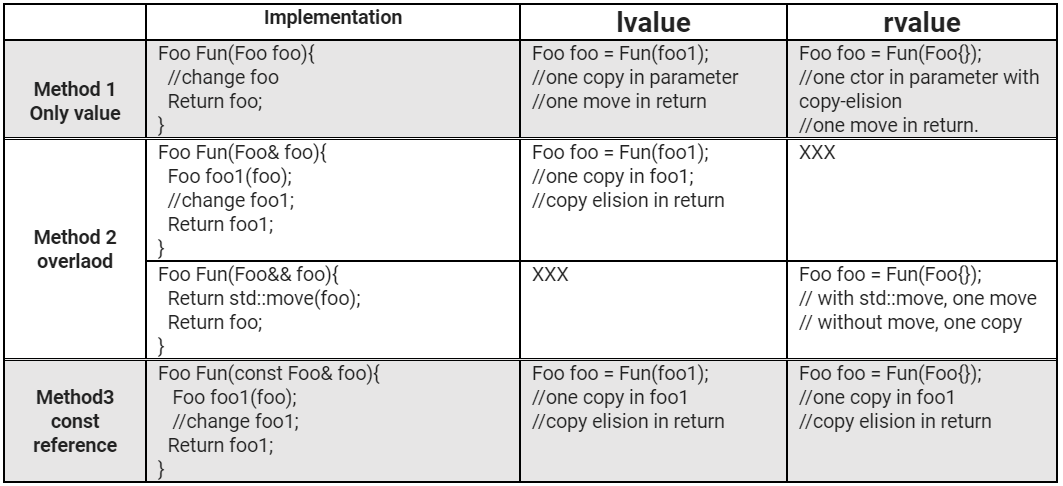
\includegraphics[scale=0.5]{pics/copy1.png}
\end{center}

\item For left value, method 1 has extra move operation.

\begin{tabular}{|c|c|c|c|}
	\hline
	left value input	& constructor & copy & move  \\
	\hline
	Method 1 & 1 & 1 & \textbf{\underline{1}} \\
	\hline
	Method 2&  1& 1 & 0  \\
	\hline
	Method 3&  1&  1& 0 \\
	\hline
\end{tabular}

\item For right value, method 1 has extra move operation, but method 3 has extra copy

\begin{tabular}{|c|c|c|c|}
	\hline
	right value input	& constructor & copy & move  \\
	\hline
	Method 1 & 1 & 0 & 2(1)  \\
	\hline
	Method 2 & 1 & 0 & 1 \\
	\hline
	Method 3 & 1 & \textbf{\underline{1}} & 0 \\
	\hline
\end{tabular}


\item Comparison of three methods. 
\begin{enumerate}
	\item For method 1 for rvalue,  if you use -fno-elide-constructors, then it use 2 move, otherwise use 1 move(Copy-elision happens when we pass the parameter into the function). Even we use 2 move, \textbf{compared with method 3, it doesn't need a copy.}
	
	\item Method 2 is the best, but you need to write two overload functions.
	
	\item For method 3, When return, you can have RVO, no copy or move when we return. Only one copy inside the function.
	
	\item If don’t use method 2.  We are taught that reference is more efficient than value(it can avoid coping). But in our specific scenario(we still copy inside the function even we use reference). \texttt{if move is cheaper than copy, then method1 is better than method 3}. Although for lvalue, It use one more move, but for rvalue, it also use move, not copy(expensive operation).
	  
\end{enumerate}


\item summary:
\begin{enumerate}
	
	\item For non-cheap-move, such as all primitive type included class, move is just like copy, \textbf{So reference WIN!}
	
	\item For c++11 and cheap-move semantic, \textbf{value WIN!} The same idea can be seen in the "more effective C++ item 41" 
	
	\item For = operator, we don't need return value, but return reference, In this way, \textbf{value WIN!}. Detail can be found in use swap to implement = operator below. \textbf{That is the famous principal four and half rule.} One copy constructor, one move ctor, one value assignment, , one destructor, one swap(half).
	
\end{enumerate}

\item You can apply this guideline immediately in assignment operators. The canonical, easy-to-write, always-correct, strong-guarantee, copy-and-swap assignment operator is often seen written this way:
\begin{lstlisting}[frame=single, language=c++]
T& T::operator=(T const& x){ 
	T tmp(x);          
	swap(*this, tmp);  
	return *this;      
}

T& operator=(T x){ 
	swap(*this, x);
	return *this;   
}
\end{lstlisting}
\begin{description}
	\item[Line 2 to 4:] \texttt{x} is a reference to the source. copy construction of tmp does the hard work. trade our resources for tmp's. our (old) resources get destroyed with tmp 
	
	\item[Line 7 to 10:] A better one is below. \texttt{x} is a copy of the source; hard work already done. trade our resources for x's. our (old) resources get destroyed with \texttt{x}.
\end{description}

\item You can't apply this idea into the copy constructor, otherwise it will cause dead recursive.
\begin{lstlisting}[frame=single, language=c++]
Class A{
	A(A a){..} //Can't declare in this way.
}
\end{lstlisting}

\item Two good articles about this topic are:"Want Speed? Pass by Value." and "WANT SPEED? DON'T (ALWAYS) PASS BY VALUE."

\subsubsection{only rvalue  reference solution}

    \item A more academic options is to just pass rvalue reference to deal with lvalue and rvalue at the same time. This idea can be googled by "Pass By Rvalue Reference Or Pass By Value"; But for lvalue, you need a help function here.
\begin{lstlisting}[frame=single, language=c++]
template<typename T>
T copy_to_temp(const T& t) { return t; }

SomeType t; 
s.initByRef(copy_to_temp(t)); //t is lvalue, need copy first.
\end{lstlisting}

    \item The same idea can be applied to move-only types (such as \texttt{unique\_ptr<T>})
\begin{lstlisting}[frame=single, language=c++]
template<typename T>
T move_to_temp(T& t) { return std::move(t); }

void foo(unique_ptr<SomeType>&& param);
unique_ptr<SomeType> p;
foo(move_to_temp(p));//note: this does move, p will become empty 
foo(std::move(p));//here, p will not become empty.  
\end{lstlisting}


    \item Frankly speaking, it's not mainstream idea, because it's a little difficult to understand and need extra help funciton. keep just for fun.

%VMore interesting example:
%\begin{lstlisting}[frame=single, language=c++]
%template<typename T>
%T move_to_temp1(T& t) { return std::move(t); }
%T&& move_to_temp2(T& t) { return std::move(t);}


%void foo(unique_ptr<SomeType>&& param);

%unique_ptr<SomeType> p;
%foo(move_to_temp1(p));  //compile ok, return value is prvalue
%foo(move_to_temp2(p));  //compile ok, return value is xvalue
%\end{lstlisting}
%\begin{description}
	%\item[Line 2:] here move constructor is called when return to a value
	%\item[Line 4:] here no move constructor is called, just reference value assignment.
%\end{description}


\subsubsection{forwarding reference}

    \item The last option is universial reference. At this time, you have to use \texttt{std::forward} 
\begin{lstlisting}[]
template<typename T>
Fraction reduceAndCopy(T&& frac){ // universal reference param
	frac.reduce();
	return std::forward<T>(frac); 
} 
\end{lstlisting}
\begin{description}
	\item[Line 4:] Have to use \texttt{std::forward<T>} here and only used in template function.
\end{description}

\end{itemize}

\section{funciton interface-return}
\subsection{funtion return basic introduction}
\begin{itemize}
	\item \textbf{These are two most important knowledge to understand function return.}
	\begin{enumerate}
		\item For no RVO, there are two steps when we return value.
		\item RVO is a kind of copy elision. In RVO implementation, we implicit pass the result by reference.
\begin{lstlisting}
X bar(){
	X xx;
	return xx;
}
	
X result = bar(); //change bar definition to below:
void bar(x &__result){
	__result.X::X() // default constructor call
	....
	return
}
\end{lstlisting}

	\end{enumerate}
	
	\item Three basic knowledges about function return when no RVO:
	\begin{enumerate}
		\item It's very important understand there are two phrases when you return from function. The first step  is from inside fun fauto to outside of function ftemp(unname tempory), then fauto disappear(call destructor for value).  Then in second step, \textbf{Move} from ftemp to flast. because ftemp is rvalue.
\begin{lstlisting}[numbers=none]
Foo fun(){
	return fauto;
}
		
Foo flast = (ftemp created here)fun();
\end{lstlisting}
		\item ftemp is not on the stack, so you can use const ref or rref to prolong its life. ftemp is same with fauto, but maybe not same with flast(Will happen implicit conversion sometimes)
\begin{lstlisting}[frame=single, language=c++]
Foo fun(){
	return fauto;
}
		
const Foo& flast = (ftemp created here)fun();
Foo&& flast = fun();
\end{lstlisting}

	\end{enumerate}
	
	\end{itemize}

\subsection{return plain reference} 
\begin{itemize}
	\item \textbf{Don't return reference or pointer to private member variables through you public member functions. It will break encapsulation. }
	
	\item Now talk about return reference: \textbf{Never return reference which refers to local variable, it will cause dangling problem.} 
	
	\item  When the client programmer does something like this and uses a reference beyond its lifetime, the bug will typically be intermittent and very difficult to diagnose. Indeed, one of the most common mistakes programmers make with the standard library is to use iterators after they are no longer valid, which is pretty much the same thing as using a reference beyond its lifetime
	
\begin{lstlisting}[frame=single, language=c++, mathescape=true]
string& a = FindAddr( emps, "John Doe" );
emps.clear(); //invlalid a here
cout << a; //a has been dangling  
\end{lstlisting}
	
	\item Why \textbf{don't} we usually return plain reference?
	\begin{enumerate}
	\item You want to return a reference to avoid copy of stack obj inside of function, but in fact it's totally wrong. We have RVO and implicit \texttt{std::move}.
	
	\item If you return non-stack obj, You have to:
		\begin{enumerate}
			\item new a obj, in this way, you can return pointer directly.
			\item input a reference for read, in this way, you can input const reference, You don't need to return it at all.
			\item input a reference for write, in this way, you don't need return it either, modification will act on inputted reference directly. So when do we use return plain reference?
		\end{enumerate}
	
	\end{enumerate}
	
	\item As far as I know, return plain reference only happens: You input a reference first, such as overload \verb=<<=. Member function return some member data, such as  assignment operator and overload \verb=[]= inside a class. \texttt{=} and \texttt{<<} are for support cascading syntactic usage: such as \texttt{cout<<a<<b}, \texttt{a=b=c}.  \texttt{[]} is for support assignment \texttt{obj[3]= 12}.  That is all.

\begin{lstlisting}[numbers=none]
operator =
operator []
operator << and >>
\end{lstlisting}
	
	\item If you want to return reference,  there is a defensible option that allows returning a reference and thus avoiding a temporary. But it's your last resort.
\begin{lstlisting}[numbers=none]
const string&
FindAddr( /* pass emps and name by reference */ ){
	for( /* ... */ ){
		if( i->name == name ){
			return i->addr;
		}
	}
	static const string empty;
	return empty;
}
\end{lstlisting}
\end{itemize}

\subsection{return rvalue reference}
\begin{itemize}
	\item \textbf{rvalue reference is also reference first, so if we have reason don't return reference from function, all these reason is also valid for rvalue reference.} The most common case for returning rvalue reference is \texttt{std::move}. It doesn't involve any move action inside the function, but is just a type cast operation.
	
	\item Return rvalue reference 1: If you want to return plain reference, or rvalue reference from a function, you have to input a plain reference or rvalue reference first, because you can't return any reference bound to local stack obj.
	
\begin{lstlisting}
A&& rrfun1(A&& arg){
	return std::move(arg);//arg is lvalue, so use move	
}
	
A&& rrfun2(A& arg){
	return std::move(arg);
}
	
A a;
A b= rrfun1(std::move(a) );
A b = rrfun2(a); // a has been moved to b. 
A&& c = rrfun2(a);
\end{lstlisting}
\begin{description}
	\item[Line 12:] will not call move constructor at all. So you mean that I want to keep watch for a while, and obj a is still intact right now.
\end{description}
 
	
	\item Return value is better than return rvalue reference.  More clear semantic. When use with auto, it's support RVO.
	
	\item Next we talk rvalue reference qualifier. Please see two examples below. More details can be googled  "C++ Gems: ref-qualifiers"
	\begin{enumerate}

		\item The ref-qualifier \&\& says that the second function is invoked on rvalue temporaries, making the following move, instead of copy
	
\begin{lstlisting}
struct Beta {
	Beta_ab ab;
	Beta_ab const& getAB() const& { return ab; }
	Beta_ab && getAB() && { return move(ab); }
	Beta_ab getAB() && { return move(ab); }
};

Beta_ab ab = Beta().getAB();
\end{lstlisting}
\begin{description}
	\item[Line 4:] return \&\& is not correct interface design. It will call move version. \texttt{Beta\_ab \&\& ab = Beta().getAB();} \texttt{ab} is dangling rref.
	\item[Line 5:] return value is correct interface.
\end{description}

			\item The same idea just like previous example, but this time I use auto.
\begin{lstlisting}[frame=single, language=c++]
DataType data() && { return std::move(values); } // why DataType?
auto values = makeWidget().data();

DataType && data() && { return std::move(values); }
auto&& values = makeWidget().data();
\end{lstlisting}
\begin{description}
	\item[Line 5:] values will be dangling because makeWidget() return value disappear.
\end{description}

	\end{enumerate}

	\item A few good articles you can dig deeper:
	\begin{enumerate}
		\item Efficiency of C++11 push\_back() with std::move versus emplace\_back() for already constructed objects.
		\item view the default functions generated by a compiler?
		\item One variable initialization form to rule them all, via mandatory elision.
		\item Episode Eleven: To Kill a Move Constructor
	\end{enumerate}

\end{itemize}

\subsection{return value-RVO}

\subsubsection{common RVO cases}
\begin{itemize}
	\item RVO is a kind of copy elision. 
	\begin{enumerate}
		\item \textbf{it happens when you return value from a function.}
		\item The type of the \textbf{local} object is the same as that returned by the function.
		\item the local object is what's being returned.
		\item parameter is not eligible for RVO. 
		\begin{enumerate}
			\item value parameter will use move in the implicitly, you don't need explicit call \texttt{std::move}.
			\item lvalue reference parameter usually should not be move, just copy.
			\item for rvalue reference, you can use std::move to move the resource to the return value.
		\end{enumerate}
	\end{enumerate}
	
	\item Four common cases of copy-elision are:
	\begin{enumerate}
		\item Name RVO, \texttt{t} has a name. It's called NRVO.
\begin{lstlisting}[numbers=none]
Thing f() {
	Thing t;
	return t;
}
Thing t2 = f();
\end{lstlisting}

		\item RVO, No name, just return temporary.
\begin{lstlisting}[numbers=none]
Thing f() {
	return Thing();
}
Thing t2 = f();
\end{lstlisting}

		\item temporary is passed by value
\begin{lstlisting}[numbers=none]
void foo(Thing t);
foo(Thing());
\end{lstlisting}

\item exception is thrown and caught by value
\begin{lstlisting}[numbers=none]
void foo() {
	Thing c;
	throw c;
}

int main() {
	try {
		foo();
	}
	catch(Thing c) {  
	}             
}
\end{lstlisting}

	\end{enumerate}

\end{itemize}

\subsubsection{RVO limitations}
\begin{itemize}
	\item Different named object sample will not trigger RVO
\begin{lstlisting}[numbers=none]
RVO MyMethod (int i){
	RVO rvo;
	rvo.mem_var = i;
	if (rvo.mem_var == 10)
		return RVO();
	return rvo; 
}
\end{lstlisting}
	
	\item returning a parameter or Global
\begin{lstlisting}[numbers=none]
Snitch global_snitch;

Snitch ReturnParameter(Snitch snitch) {
	return snitch; //no RVO here
}

Snitch ReturnGlobal() {
	return global_snitch; //no RVO here either
}
\end{lstlisting}

\item return by std::move(). \textbf{That is the most obvious error for some basic C++ developers, who do understand RVO very well.} 
\begin{lstlisting}[numbers=none]
Snitch CreateSnitch() {
	Snitch snitch;
	return std::move(snitch);
}
\end{lstlisting}
	
\item In some cases even an unnamed variable can't RVO:
\begin{lstlisting}[numbers=none]
struct Wrapper {
	Snitch snitch;
};

Snitch foo() {
	return Wrapper().snitch;
}

int main() {
	Snitch s = foo();
}
\end{lstlisting}

\end{itemize}

\subsubsection{Some practical demos and analysis}
\begin{itemize}
	
	\item Given below code as experiment code:
\begin{lstlisting}[frame=single, language=c++]
class Snitch {   // Note: All methods have side effects
	Snitch() { cout << "c'tor" << endl; }
	~Snitch() { cout << "d'tor" << endl; }
	
	Snitch(const Snitch&) { cout << "copy c'tor" << endl; }
	Snitch(Snitch&&) { cout << "move c'tor" << endl; }
	
	Snitch& operator=(const Snitch&) {
		cout << "copy assignment" << endl;
		return *this;
	}
	
	Snitch& operator=(Snitch&&) {
		cout << "move assignment" << endl;
		return *this;
	}
};
	
Snitch CreateSnitch() {
	return Snitch();
}
	\end{lstlisting}
	
	\item test 1 and output 
\begin{lstlisting}[frame=single, language=c++]
int main() {
	Snitch s = CreateSnitch();
}
\end{lstlisting}
\begin{description}
	\item[Output:] The compiler switch and its output:
	\begin{verbatim}
		with -fno-elide-constructors
		c'tor    //Snitch()
		move c'tor  //Snitch() to return value
		d'tor       //Snitch() destroy
		move c'tor //return value to s
		d'tor     //return value destroy
		d'tor     //s destroy
	------------------------------
		without -fno-elide-constructors
		c'tor   //s
		d'tor   //s destory
	\end{verbatim}
\end{description}
	
	\item test 2 and output
	\begin{lstlisting}[frame=single, language=c++]
int main() {
	Snitch s;
	s = CreateSnitch();
}
	\end{lstlisting}
\begin{description}
	\item[Output:] The compiler switch and its output:
	\begin{verbatim}
		with -fno-elide-constructors
		c'tor    //Snitch s
		c'tor    //Snitch() in side CreateSnitch
		move c'tor  //Snitch() to return value
		d'tor       //Snitch() destory
		move assignment //return value to s
		d'tor     //return value destory
		d'tor     //s destory
	----------------------	
		without -fno-elide-constructors
		c'tor   //Snitch s
		c'tor   //Snitch()
		move assignment //s has been implicit passed to CreateSnitch, 
		//so s = Snitch() happen inside CreateSnitch
		d'tor   //Snitch() destory
		d'tor   //s destory
	\end{verbatim}
\end{description}

	\item test 3 and output
\begin{lstlisting}[frame=single, language=c++]
Snitch CreateSnitch() {
	return Snitch();
}
	
Snitch CSnitch(Snitch&& rs) {
	return rs;
}
	
int main() {
	Snitch s = CSnitch(CreateSnitch());
}
\end{lstlisting}
\begin{description}
	\item[Output:] The compiler switch and its output:
	\begin{verbatim}
		with -fno-elide-constructors
		c'tor    //
		copy c'tor    //
		d'tor       /
		copy c'tor    //
		copy c'tor    //
		d'tor       /
		d'tor     //r
		d'tor     //
	-------------------------
		without -fno-elide-constructors
		c'tor   //Snitch s
		copy c'tor //
		d'tor   //Snitch() destory
		d'tor   //s destory
	\end{verbatim}
\end{description}
\end{itemize}


\subsubsection{RVO and move}
\begin{itemize}
	
	\item A common error is when there is no RVO, use \texttt{std::move} to avoid copy: but Although parameter is not eligible for RVO, or different path is not eligible, but you don't need to explicit use \texttt{std::move}, the compiler will use them implicitly.
	
\begin{lstlisting}
Widget makeW(Widget w){
	.....
	return w
	//return std::move(w), don't do it. compiler call move. 
} 
\end{lstlisting}
	
	\item If a function is \textbf{value return}, and you want to return \textbf{a rvalue reference parameter}, you have to use move in the return.
	\begin{enumerate}
		\item \textbf{lhs is not local object, but reference, so No RVO}
		\item you may say: but lhs is rvalue reference, but lhs is name rvalue reference. It's lvalue.
		
		\item Just like you pass a lvalue reference, you can't move it unless you want to do it explicitly. That is why we need \texttt{std::move} here. Frankly speak, this is typical example to demonstrate when you can use \texttt{std::move} when you return value, so I recommend you to remember it.
	\end{enumerate}

\begin{lstlisting}[frame=single, language=c++]
Matrix operator+(Matrix&& lhs, const Matrix& rhs){
	lhs += rhs; 
	return std::move(lhs); //move into return value, high efficiency. 
	//return lhs  //will copy, so low efficiencey
} 
\end{lstlisting}

\end{itemize}

%\subsubsection{return mulit value}
%\begin{itemize}
	%\item You can return pair, tuple and variant. 
	%\item for example, map.insert just return a pair. 
	%\item how to use variant as return value? find a example here
%\end{itemize}

\subsection{Function return design summary}

\begin{itemize}
		\item \textbf{In Summary 1, Three operator overload return plain reference, one std::move return rvalue reference. It doesn't involve value semantic, just a type change. All the others return value, That's all!}
	
		\item \textbf{In summary 2, If function return value, For only copy lvalue, return value; for rvalue reference, move;  For universal reference, forward. } For rvalue reference parameter, you should use \texttt{std::move} explicitly. Because it's name rvalue reference, at the same time, it's a reference, not local auto object, if we don't use \texttt{std::move}, we will copy it when we return it.  Apply \texttt{std::forward} to universal references the last time each is used.
	
\begin{lstlisting}[numbers=none]
Matrix operator+(Matrix& lhs, const Matrix& rhs) {
	return lhs //for lvalue refence, return it .
}
	
Matrix operator+(Matrix&& lhs, const Matrix& rhs) {
	return move(lhs) //for rvalue reference, move it.
}
	
template<type T>
T operator+(T&& lhs) {
	return forward<T>(lhs) //for forwarding reference, forward it.
}
\end{lstlisting}

		\item \textbf{Try to use RVO first, no move and copy at all.} Never apply \texttt{std::move} or \texttt{std::forward} to local value objects if they would otherwise be eligible for the return value optimization.

		\item For a local stack variable, if RVO doesn't perform, compiler will implicit use \texttt{std::move} instead copy, so please don't use \texttt{std::move} on the local stack variable either.

		\item \textbf{if RVO is not applicable, at the same time, move is not cheap, we should use referent parameter as return methond, such as big POD type, or use it in loop.} I think that it will be rare case. If you have good example of this, please tell me. 

\end{itemize}

\subsection{Summary of function interface design}
\begin{itemize}
		\item The main idea of function interface design can be see in the below figure:
	\begin{figure}[h]
	\centering
	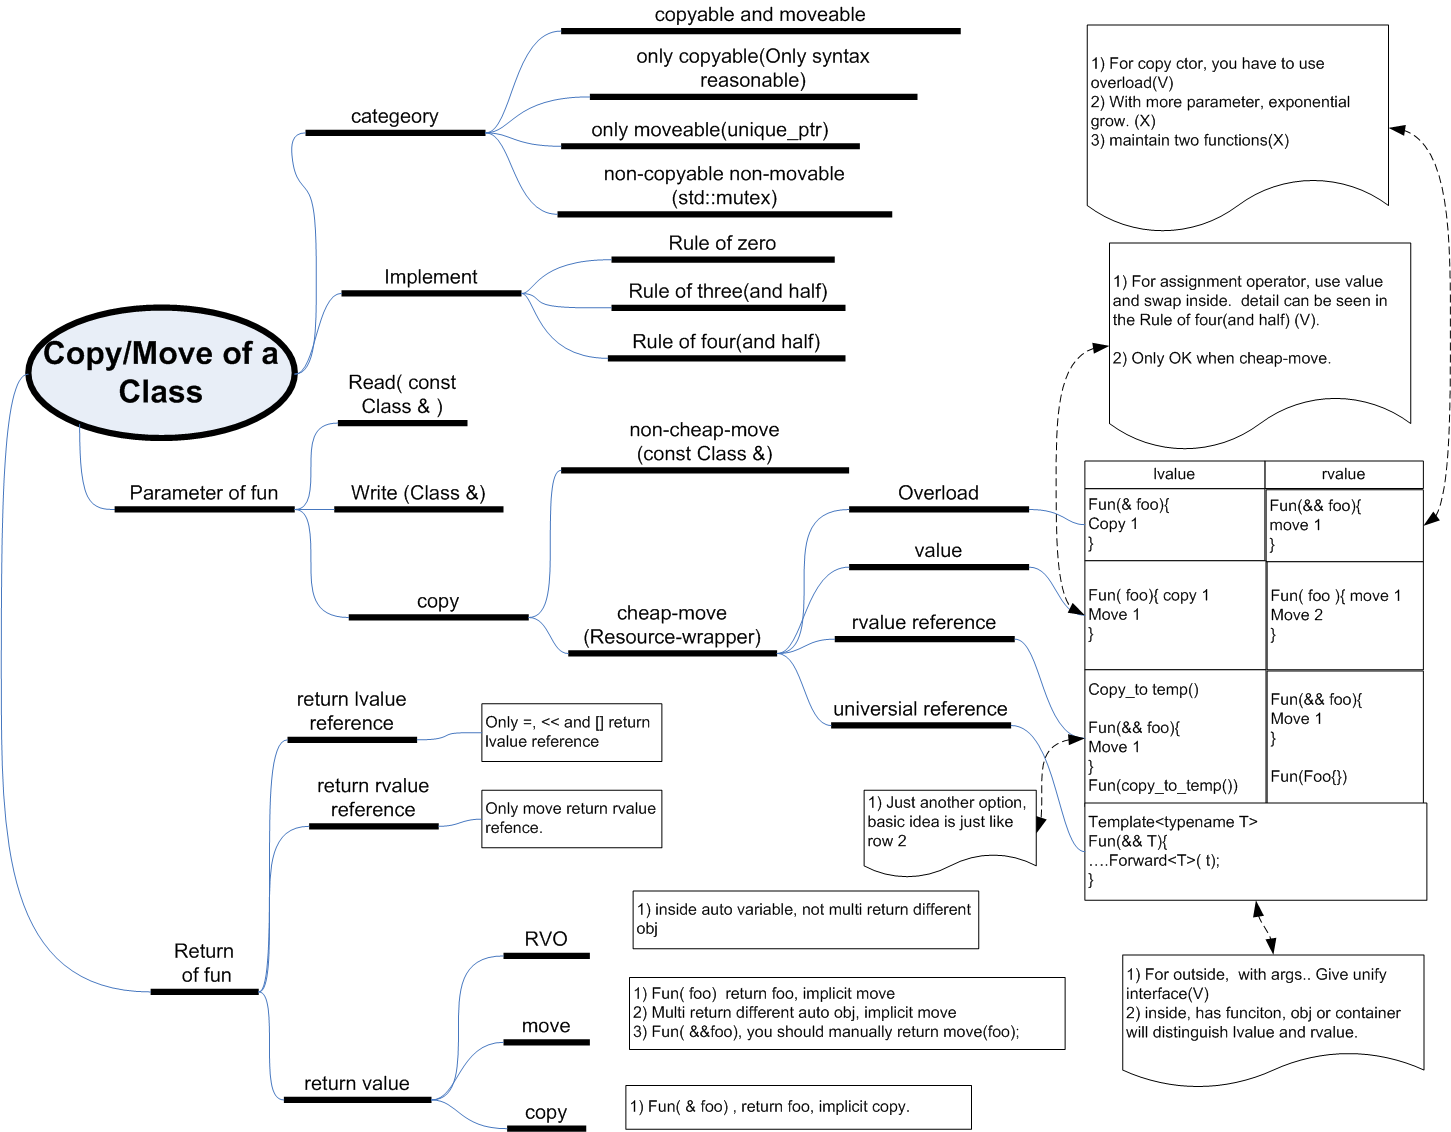
\includegraphics[width=1.0\linewidth]{pics/move.png}
	\caption{rvalue reference and function interface.}
	\label{fig:rvalueref}
	\end{figure}

\end{itemize}

\section{Summary of the chapter}
\begin{enumerate}
		\item First, we introduce value categories and lvalue and rvalue.
		\item Second, based on rvalue, we introduce rvalue can pick up const lvalue reference in function overload resolution. 
		\item Third, we invent rvalue reference to only bind rvalue.
		\item With rvalue refence, we also invent name rule, unname rvalue reference is rvalue.( \texttt{std::move} use this rule.) 
		\item Another problem arise, is \texttt{std::move} return lvalue or rvalue? So we invent a new value category, xvalue, and change rvalue = (prvalue+xvalue).

		\item Then for some forward context, we invent forward reference and refernce collapse rule to deal with this problem. That is the whole picture of this chapter.
				
		\item With above new conceptions, we talked about how to design function interface, the main two parts are parameters design and return value design. 
\end{enumerate}

\chapter{OOP}

\section{Object basic}

\subsection{class categories}
\begin{itemize}
	\item Basic class categories:
	\begin{enumerate}
			
		\item Value-like types, such as \texttt{int} or \texttt{vector<widget>}. These represent values, and should naturally be copyable. In C++11, generally you should think of move as an optimization of copy, and so all copyable types should naturally be moveable... moving is just an efficient way of doing a copy in the often-common case that you don't need the original object any more and are just going to destroy it anyway. such as \texttt{std::pair} \texttt{std::vector} and \texttt{std::string}.
		
		\begin{enumerate}
			\item Has a public destructor, copy constructor and assignment operator with value semantics.
			\item Has no virtual function. so intended to be used as a concrete class, not as a base class.
			\item instantiated on stack or as a member of an other class.
		\end{enumerate}
		
		\item Reference-like types that exist in inheritance hierarchies, such as base classes and classes with virtual or protected member functions. These are normally held by pointer or reference, often a base* or base\&, and so do not provide copy construction to avoid slicing; if you do want to get another object just like an existing one, you usually call a virtual function like clone. These do not need move construction or assignment for two reasons: They're not copyable, and they already have an even more efficient natural "move" operation -- you just copy/move the pointer to the object and the object itself doesn't have to move to a new memory location at all.
		\begin{enumerate}
			\item Has a destructor that is public and virtual, But for some trait class, destructor can be protected, such as \texttt{std::unary\_function}
            \item Establish interfaces through virtual functions.
			\item \textbf{Usually instantiated on heap, and used via a (smart) pointer or reference to support polymorphism.} 
        \end{enumerate}
		

    \item Policies are classes (or class templates) to \textbf{inject behavior} into a parent class, typically through inheritance. Through decomposing a parent interface into orthogonal (independent) dimensions, policy classes form the building blocks of more complex interfaces. An often seen pattern is to supply policies as user-definable template (or template-template) parameters with a library-supplied default. An example from the Standard Library are the Allocators, which are policy template parameters of all STL containers. Policy classes (normally templates) are fragments of pluggable behavior.
        \begin{enumerate}
            \item May or may not have state or virtual functions.
            \item Is not usually instantiated standalone, but only as a base or member. 
        \end{enumerate}

\begin{lstlisting}[numbers=none]
template<class T,class Allocator=
			std::allocator<T> > class vector;
\end{lstlisting}
	
	\item Traits are class templates to \textbf{extract properties} from a generic type. There are two kind of traits: single-valued traits and multiple-valued traits. Examples of single-valued traits are the ones from the header <type\_traits>. Single-valued traits are often used in template-metaprogramming and SFINAE tricks to overload a function template based on a type condition. \texttt{std::unary\_function} is also a kind of trait class.  A type trait is a simple template struct that contains a member constant, which in turn holds the answer to the question the type trait asks or the transformation it performs. For example, let's take a look at \texttt{std::is\_floating\_point}. Another usage is like \texttt{std::remove\_reference}, it is a type trait that alters the type T it takes in input:

		\begin{enumerate}
			\item Contain only typedef and static functions, It has no modifiable state.
			\item Is not instantiated( constructor is private or disable)
		\end{enumerate}
	\begin{lstlisting}[numbers=none]
template< class T >
struct is_integral{
	static const bool value
	/* = true if T is integral, false otherwise */;
	typedef std::integral_constant<bool, value> type;
};
	
template <class T>
T f(T i){
	static_assert(
		std::is_integral<T>::value, "Int required.");
	return i;
}

int main() {
	std::cout << f(123) << '\n'; //output 123
}
\end{lstlisting}

    \item exception class. They are thrown by value but should be caught by reference. 

		\item Ancillary classes typically support specific idioms. such as RAII.  types that express unique ownership of a resource, such as \texttt{std::unique\_ptr}, are naturally move-only types, because they are not value-like (it doesn't make sense to copy them) but you do use them directly (not always by pointer or reference) and so want to move objects of this type around from one place to another.	

        \item Functor class, includes lambda. with operator() defined. This becomes more and more importants and win a seat in this list. 
	\end{enumerate}
    \item About class categories, I need to have a few points to add. Most of time, we mainly use value object and reference object. The others kinds are a kind of special and easy to understand. For value object, you can think that it's a \textbf{data abstraction}, which has zero or very little overhead. 
    \item For reference object, usually we don't support copy, for example, A people object has no meaning to copy himself. It has three points need to metion:
        \begin{enumerate}
            \item It it's only used for interface, so it will be Abstract Base Class. There are two common idioms can be used here: NVI(No virtual interface) and Non-leaf-abstraction. Detail can be see later in design section. 

            \item non-copyable child class. such as thread, employee etc. You should disable the copy constructor when you find it's not fit into the context.

            \item copyable child class. A good example is music note, You can see the clone pattern in design pattern. Here music note is a kind of interface. So it's a ABC, at the same time, client should be able to "copy" to generate new notes. Under such context, you can use virtual copy constructor, in another word, use \texttt{basePtr->clone()} virtual function. Clone pattern is just for this scenario. 

        \end{enumerate}
\end{itemize}

\subsection{Friend}

    \begin{itemize}
        \item Keep in mind that only a class declaration can decide which functions are friends, so the class declaration still controls which functions access private data.
        \item  Friend has three categories:

	\begin{enumerate}
		\item Friend Class: just as TV and RemoteControl, you can declare RemoteControl a friend class inside TV.
		
		\item Friend Member functions: You can select some member functions to be friend of another class, In this way, you need forward declaration.  
		
		\item Common Friend method, a good example is overload \verb=operator <<=. 
	\end{enumerate}

    \end{itemize}

\subsection{Class interface design}
\begin{itemize}
	
	\item Nesting a class does not create a class member of another class. Instead, it defines a type that is known just locally to the class that contains the nested class declaration.  A good example is Class queue nest class node,  because node is just used inside the class Queue. Another good example is vector and it's iterator.
	
	\item Virtual function must be member, operator\verb=>>= and \verb=<<= are never be members, or It maybe be a friend. Only non-member functions get type conversions on their left-most argument.  In the previous example, If you want to use support \texttt{2*obj}, You need make operator * to be non member function.  Detail can be seen in effective c++.
	
	\item Protect keyword don't use very often, it is just used in inheritance context. Child class can access base class protected member. you should use private keyword first if you real want to have good \textbf{Encapsulation} and \textbf{Never return reference or pointer to a private or protected member data.}
	
	\item In C++ primer p653, you can see a good example class interface. You should remember it as a basic pattern.  If you use new operator to allocate memory inside of your class, you should define: copy constructor, assignment operator and destructor, move copy ctor, and move assignment.
	
\begin{lstlisting}[frame=single, language=c++]
//below is string.h file
#pragma once
namespace Yan{
	class String{
	public:
		String();  //default constructor
		String(const char *a ); // specify constructor
		
		String (const String &);  //copy constructor
		String (String && other); //move copy constructor
		
		String& operator=(const String &); //assignment
		String& operator=(String&& other); //move assignment
		String& operator=(const char*a); // option.
		
		~String();  
		
		friend ostream& operator<<(ostream & os, const String & st);
		friend istream& operator>>(istream & is, String &st);
		
	private:
		const static int NUM= 1000; // const used inside of this class.
		char* m_str;
		
	};
	ostream& operator<<(ostream & os, const String & st);
	istream& operator>>(istream & is, String &st);
}
\end{lstlisting}
\begin{description}
    \item[Source code:] From Line 1 to Line 16: usually, you should have these seven member functions. Or you can follow the Principal Four and Half rule which will be introduced later.  Put class definition into a namespace. You need to declare operator \verb=<<= inside of namespace outside of class. In this way, ADL can access it correctly.
\end{description}

        \item \texttt{String\& operator=(const char*a);} is an option, why it make \texttt{str=temp} more efficient? see C++ Primer P652.
	
\begin{lstlisting}[numbers=none]
String str; char temp[40];
str= temp // make it more efficient
\end{lstlisting}
	
	
    \item \textbf{Prefer minimal classes to monolithic classes.} Big class is difficult to reach error-safe because it tackle multiple responsibilities. It's also difficult maintain, understand and deploy.

	\item member or non-member function?
	\begin{enumerate}
		\item operator =, ->, [], () must be members.
		\item needs a different type as its left-hand arguent, such as operator \verb=<<=, use nonmember.
		\item leftmost argument needs type conversion, use non-member.
		\item can be implement using the class public interface alone, use nonmember.
	\end{enumerate}

	\item Prefer non-member non-friend functions. A good example is begin function in STL. non-member style can be used in generic programming better.  

\begin{lstlisting}[numbers=none]
std::vector<int> vi = {1,2,3};
auto i = vi.begin();
auto i = begin(vi);
\end{lstlisting}
	
\end{itemize}

\section{Object base}
\subsection{Constructor}

\subsubsection{constructor basic}

\begin{itemize}
	\item Normally, constructor, destructor and assignment should be public. Unless you have special requirment for special class or in special context. Avoid calling virtual functions in constructor and destructor. Detail can be found in "C++ Coding Standards" item 49.
	
	\item Make Constructors Protected to prohibit direct instantiation. Make constructors Private to stop Derivation. That is an old trick, in C++ 14, you can use \texttt{=delete} to tell compiler directly.
	
	\item Use default arguments to reduce the number of constructor.
\begin{lstlisting}[numbers=none]
class Brush{
	Brush();
	Brush(Color c);
	Brush(Texture t);
	Brush(Color c= Black,Texture t=Solid); //better
}
\end{lstlisting}
		
		\item A copy constructor is called whenever a new variable is created from an object. This happens:
		
		\begin{enumerate}
			\item When a new object is initialized to an object of the same class.
			\item When an object is passed to a function by value.
			\item When a function returns an object by value.
			\item When the compiler generates a temporary object.
		\end{enumerate}
		
		\item In previous example, you can see when you pass value of obj, It will call copy constructor, It's not very efficient. So you should use reference or pointer if it's possible, don't pass object directly.
		
		\item For reference, once assigned, a reference cannot be re-assigned. So if a class has a reference member, It can be initialized by initializer list in constructor and copy ctor. \textbf{But you can't overload assignment operator any more, If you really need assignment operator, change reference to pointer}
		
\end{itemize}

\subsubsection{default constructor}
\begin{itemize}
	
	\item Avoid gratuitous default constructor. If an object can be generated from "nothing", maybe you can give a default constructor, such as a container, you can generate an empty container without any input. 

	\item \textbf{If you define a specific constructor, system will not produce any default ctor for you.} At this time, maybe you need to add default constructor.
	
	\item For container example, default constructor is reasonable, you can declare your own converting constructor and use system implicit generated one. you can use keyword default
\begin{lstlisting}[frame=single, language=c++]
class Container{
	Empty() = default;
	Empty(int size) ;
}
\end{lstlisting}

	\begin{description}
		\item[Line 2:] you don't need to give implementation of default constructor.
	\end{description}
	
	
	\item But for others classes, \textbf{you should not generate a object from nothing}. For example, You must provide SSN when you create a worker. At this time, if you create default constructor, It's not good idea. A NULL SSN will cause a lot of trouble in the future. 
\begin{lstlisting}[numbers=none]
class Worker{
	char* SSN; // each worker should have SSN
	Worker(const char*);
	Worker(){SSN=nullptr); //bad smell.
}
\end{lstlisting}
	
	\item We should not declare default constructor, in this way, our class design represents real word better. But without default constructor, all below statements will produce errors when compiling.
	
\begin{lstlisting}
class Worker{
	char* SSN;
	Worker(const char*); 
};

Worker obj; //error
Worker* obj = new class(); //error
Worker arra[10] //error
template<class T>
class Array{
	T t;
};

Array<Worker> a; //error
\end{lstlisting}
\begin{description}
	\item[Line 3:] User-declared constructor stop system from generating default constructor.
\end{description}

	
    \item In this way, you have to use \texttt{Worker*} pointer, or \texttt{vector<Worker>}.  You can also use \texttt{=delete} to disable default constructor. That is C++ spirit, \textbf{You never have the best answer, only have context answer. }

\item summary:
\begin{enumerate}
	\item Any user-declared converting constructor will stop compiler from generating default constructor.

	\item If default constructor satisfy class semantic, such as container class, you can add it by you self.

	\item If default constructor is not valid for class semantic, such as Worker class, you should not declare explicitly. 

	\item Absence of default constructor bring some inconvenient. Such as you can't define a array of this class. \texttt{Worker arr[10];} 
\end{enumerate}
	
\end{itemize}

\subsubsection{member initializer list}

\begin{itemize}
	\item \textbf{Always use member initializer list instead of assignment inside constructor.}
	
	\item When to use member initializer list?
	\begin{enumerate}
		\item to non-static const data members.
		\item reference member
		\item  member objects which do not have default constructor: (why I need default constructor can be explained here too)
		\item need pass argument to base class constructor
\begin{lstlisting}[numbers=none]
class A {
public:
	int i;
	A(int );
};
class B: A {
public:
	B(int );
};
	
B::B(int x):A(x) { //Initializer list must be used here.
    cout << "B's Constructor called";
}
\end{lstlisting}		
		
		\item need to by copy between obj to member obj. (only one copy constructor, more efficient! see below source code.)

\begin{lstlisting}[frame=single, language=c++]
//method 1:
class(string &a, string &b): m_a(a),m_b(b){};
		
//method 2:
class(string &a, string &b){   
	m_a = a;  
	m_b = b; 
};
\end{lstlisting}
	\begin{description}
		\item[Line 2:] just call string copy constructor, so you don't need string default ctor.
		\item[Line 6:] two action. call default constructor to build \texttt{m\_a.} then call assignment operator.
	\end{description}

	\end{enumerate}

	
	
	\item List member in a initialization list in the order in which they are declared in class. see effective c++ item 13. Order is important. Member variables are always initialized in the order they are declared in the class definition. The order in which you write them in the constructor initialization list is ignored.  \textbf{So you'd better not have one member's initialization depend on other members}.
	
\begin{lstlisting}[numbers=none]
class Student{
	string m_email;  //m_email will be init first, ingore order
	string m_first_name;  // in the constructor initialization list.
	Student(first_name) :m_first_name(first_name),
	m_email(m_first_anme+"@gmail"){}
\end{lstlisting}
		
		
		\item If \texttt{GetType()} is a static member function, or a member function that does not use its this pointer (that is, uses no member data) and does not rely on any side effects of construction (for example, static usage counts), then this is merely poor style, but it will run correctly. Otherwise (mainly, if GetType() is a normal nonstatic member function), we have a problem. \textbf{Nonvirtual base classes are initialized in left-to-right order as they are declared}, so ArrayBase is initialized before Container. Unfortunately, that means we're trying to use a member of the not-yet-initialized Container base subobject. Order is important!
		
\begin{lstlisting}[numbers=none]
template<class T>
class Array : private ArrayBase, public Container{
public:
	Array( size_t startingSize = 10 ): Container( startingSize ), 
	ArrayBase( Container::GetType() ){
		....
\end{lstlisting}
		
    \item A very good introduction about this topic can be found below:	
	\begin{verbatim}
		http://www.geeksforgeeks.org/when-do-we-use-initializer-list-in-c/
	\end{verbatim}

	\end{itemize}

\subsubsection{named constructor idiom}
\begin{itemize}
	\item First, let take a look common pattern of constructor, constructor is different, you have to use the same name. But it can't express semantic behind the function interface.
\begin{lstlisting}
class Point {
public:
	Point(float x, float y);     
	// Rectangular coordinates
	Point(float r, float a);  //error, duplicated definition. 
	// Polar coordinates (radius and angle)
};
\end{lstlisting}

\item In order to resolve this problem, we can use "named constructor". 
\begin{lstlisting}
class Point {
public:
	static Point rectangular(float x, float y);
	static Point polar(float radius, float angle);
	
Point p1 = Point::rectangular(5.7, 1.2);
Point p2 = Point::polar(5.7, 1.2);
\end{lstlisting}

\subsubsection{virtual constructor idiom}
	
	\item In some applications, we need to copy or assignment by base class pointer. For example, If the class "owns" the object pointed to by the (abstract) base class pointer which is illustrated below. (Another example can be found in More effective C++ item 25). The problem is how we can assignment and copy between Graph object? 
	
\begin{lstlisting}
class Graph {
public:
	Graph(const Graph& f)
	: p_(f.p_->clone()) { }
	
	Graph& operator= (const Graph& f){
		if (this != &f) {              
			Shape* p2 = f.p_->clone();   
			delete p_;                   
			p_ = p2;
		}
		return *this;
	}
	// ...
private:
	Shape* p_; 
};
\end{lstlisting}
\begin{description}
	\item[Line 1:] Graph can contain a shape, this shape can be squre, circle... So we use \texttt{Shape*}. 
	\item[Line 6 to 8:] Check for self-assignment; Create the new one FIRST; THEN delete the old one.
	\item[Line 16:]  \textbf{Please note here: Shape here represent value semantic and reference semantic at the same time.} If we use \texttt{Shape*->draw}, then it's reference semantic. It's also a value member inside the graph class, that is why we need to clone function for it.
\end{description}

	\item A constructor shall not be virtual or static. If you need something like this, you can look up the virtual constructor idiom. The idiom uses virtual clone() member function (for copy constructing), or a virtual create() member function (for the default constructor). The purpose is to resolve the problem of assignment and copy between Graph object. As usual with this idiom, we declare a pure virtual clone() method in the base class. It follow 'non-leaf class abstract' rule.
	
\begin{lstlisting}
class Shape {
public:
	virtual ~Shape() { }                 
	virtual void draw() = 0;           
	virtual void move() = 0;
	// ...
	virtual Shape* clone()  const = 0;   
	virtual Shape* create() const = 0; 
};
	
class Circle : public Shape {
public:
	Circle* clone()  const;  
	Circle* create() const;   
};

Circle* Circle::clone()  const{
	return new Circle(*this); }
	
Circle* Circle::create() const{
	return new Circle();      }
	
Shape* s2 = s.clone();
Shape* s3 = s.create();
	
delete s2;    // You need a virtual destructor here
delete s3;
\end{lstlisting}
	\begin{description}
		\item[Line 13 and 14:] Covariant Return Types; Virtual function can have different return type. Line 7 return \texttt{shape*}, In line 13, we can change it to \texttt{Circle*}. That is OK in C++ language.
	\end{description}


\end{itemize}


	
\subsection{destructor}
\begin{itemize}
	\item \textbf{In inheritance context, all the base class destructor should be public and virtual. Or protected and non-virtual.}  

\begin{lstlisting}[numbers=none]
class Base {
public:
	int num;
	Base(int n):num(n){
		cout<<"Base::Constructor\n";
	}
	virtual ~Base(){   //Here must declare virtual
		cout<<"Base::Destructor\n";
	}
};

class Derived : public Base {
private:
	float money;
public:
	Derived(int n, float m):Base(n),money(m){
		cout<<"Derived::Constructor\n";
	}
	~Derived(){   //you can omit virtual here,better style is to add virtual!
		cout<<"Derived::destructor\n";
	}
};


Base *base_ptr = new Derived(1,200.0);
delete base_ptr;
\end{lstlisting}

\begin{description}
	\item[Source code:] output is below: 
\begin{verbatim}
Base::Constructor                                                                                               
Derived::Constructor
Derived::destructor                                                                        
Base::Destructor 
\end{verbatim}
		\item[Source code:] if you don't declare base destructor virtual, the output will be:
\begin{verbatim}
Base::Constructor                                                                                               
Derived::Constructor                                                                        
Base::Destructor 
\end{verbatim}
	
\end{description}

	\item \textbf{Base class destructor will be called by child class destructor implicitly}, so please always implement base class destructor, even it's pure virtual. 
\begin{lstlisting}[numbers=none]
class Base {
	virtual ~Base() = 0;
};
Base::~Base(){} //Must give implementation, even function is empty. 
\end{lstlisting}	
	
	\item Prevent exception from leaving destructors.
	
	\item Normally you will have to explicitly declare your own destructor if:

	\begin{enumerate}
		\item When you are declaring a class which is supposed to serve as a base for inheritance involving polymorphism, need a virtual destructor to make sure that the destructor of a Derived class is called upon destroying it through a pointer/reference to Base.
		
		\item You need to release resourced required by the class during its lifetime. Example 1: The class has a handle of a file, this needs to be closed when the object is destroyed; the destructor is the perfect location. Exempel 2: The class owns an object with dynamic-storage duration, since the lifetime of the object can potentially live on long after the class instance has been destroyed you'll need to explicitly destroy it in the destructor.
	\end{enumerate}
\end{itemize}

\subsection{member functions relationship}

\subsubsection{Basic introduction}

\begin{itemize}

\item When you write an empty class, compiler will produce at least six member functions.  New compiler will produce move constructor and move assignment too.
\begin{lstlisting}[numbers=none]
class Empty{};

Empty();
Empty(const Empty& rhs);
Empty& oprator=(const empty & rhs);
Empty* operator&(){return this};
const Empty* operator&() const ;
~Empty();
\end{lstlisting}

\item Why do you need to pay attention to these special member functions?  Given half a chance, the compiler will write them for you. Another reason is that C++ by default treats classes as \textbf{value-like types}, but not all types are value-like. Know when to write and disable them make you get correct code.

\item A good reference is "Everything You ever wanted to know about move semantics" in slideshare.net.

\item For these special member functions, main operations can be:
\begin{enumerate}
\item Compiler implicitly declare one.
\item Use explicitly declare one.
\item Once you define one, Compiler maybe Not declare another.
\item You can ask compiler declare or delete one.
\end{enumerate}

\item First question is what "declare" mean?  \\
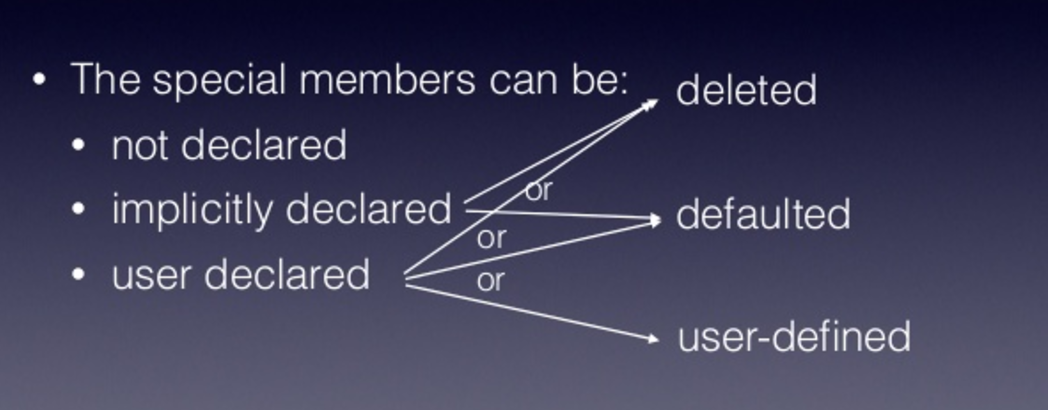
\includegraphics[scale=0.6]{pics/sm1.png} \newline

\item If you just define a class without any special member function, all six member function will be declared by compiler implicitly. \\
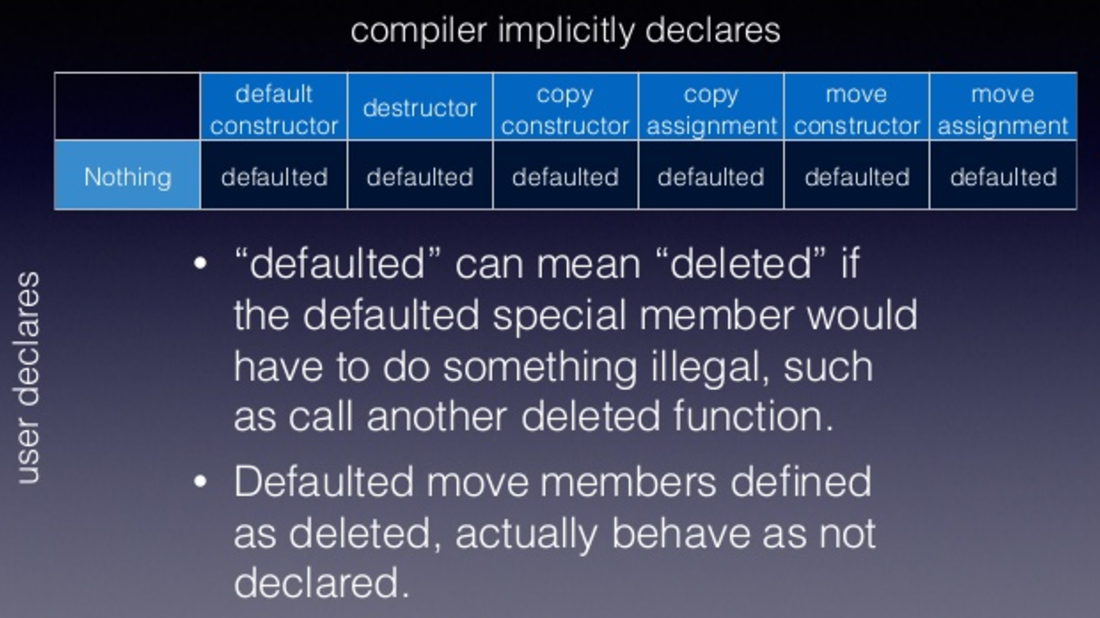
\includegraphics[scale=0.5]{pics/sm2.png} \newline


\item Default can mean "deleted", See an example below:

\begin{lstlisting}[frame=single, language=c++]
class A{
	A() = delete;
};
class B{
	A a;
};
int main(){
	B b;
}
\end{lstlisting}
\begin{description}
	\item[Output:] main.cpp:8:7: note: 'B::B()' is implicitly deleted because the default definition would be ill-formed:
\end{description}


    \item Steps of generating special member function. 
\begin{center}
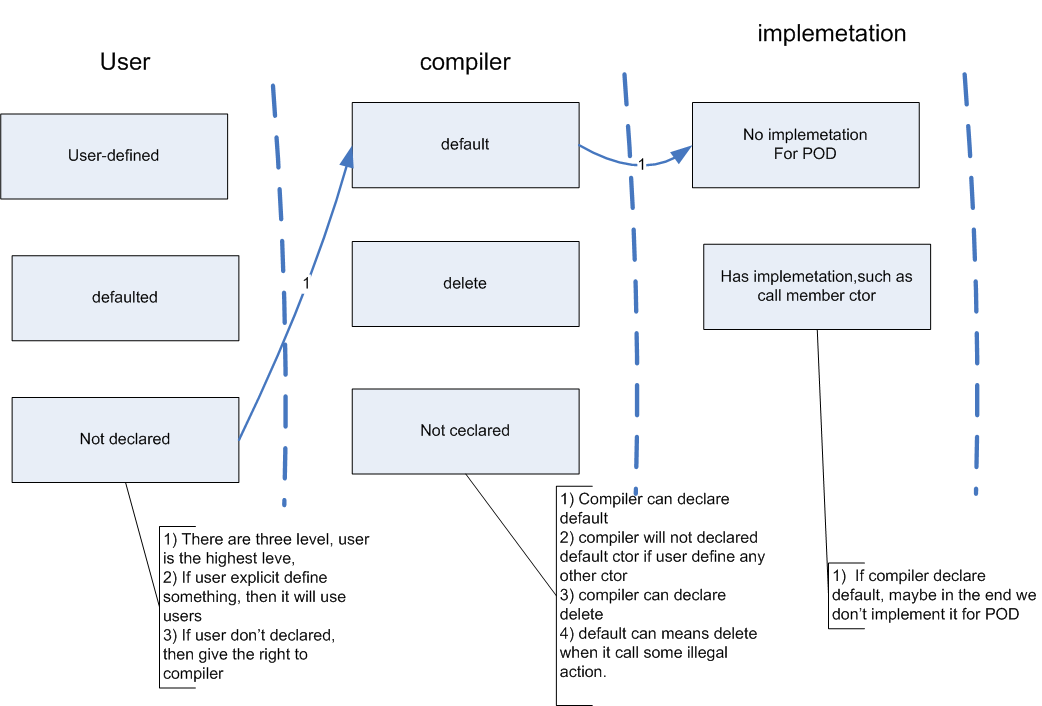
\includegraphics[scale=0.8]{pics/ctor.png} 
\end{center}
\item Next question is what differences are between \verb|=default| and user define empty constructor? problems of below code snippet are:
\begin{lstlisting}[numbers=none]
struct noncopyable  {
	noncopyable() {};
private:
	noncopyable(const noncopyable&);
	noncopyable& operator=(const noncopyable&);
};
\end{lstlisting}
\begin{enumerate}
	\item The copy constructor has to be declared privately to hide it, but because it's declared at all, automatic generation of the default constructor is prevented. You have to explicitly define the default constructor if you want one, even if it does nothing.

	\item Even if the explicitly-defined default constructor does nothing, it's considered non-trivial by the compiler. \textbf{It's less efficient than an automatically generated default constructor and prevents noncopyable from being a true POD type.}

	\item Even though the copy constructor and copy-assignment operator are hidden from outside code, the member functions and friends of noncopyable can still see and call them. If they are declared but not defined, calling them causes a linker error.

	\item Although this is a commonly accepted idiom, the intent is not clear unless you understand all of the rules for automatic generation of the special member functions.
\end{enumerate}


\item C++11 new keyword default and delete give below advantages:
\begin{lstlisting}[numbers=none]
struct noncopyable  {
  noncopyable() =default;
  noncopyable(const noncopyable&) =delete;
  noncopyable& operator=(const noncopyable&) =delete;
};
\end{lstlisting}

\begin{enumerate}
	\item Generation of the default constructor is still prevented by declaring the copy constructor, but you can bring it back by explicitly defaulting it.

	\item Explicitly defaulted special member functions are still considered trivial, so there is no performance penalty, and noncopyable is not prevented from being a true POD type.

	\item The copy constructor and copy-assignment operator are public but deleted. It is a compile-time error to define or call a deleted function.

	\item The intent is clear to anyone who understands =default and =delete. You don't have to understand the rules for automatic generation of special member functions.
\end{enumerate}

	\item Another question is what differences are between =delete and "not declare"
\begin{lstlisting}
struct X{
	template<class ...Args>
		X(Args&& ...args);
	X() = delete
};

X x 
\end{lstlisting}
\begin{description}
	\item[Source code:] Deleted members participate in overload resolution. Member not-declared do not participate in overload resolution.	
	\item[Line 7:] If we don't have line 4, The Line 7 will call template function, but if we use = delete, Line 7 stops compiler.  
\end{description}

    \item Prefer deleted functions to private undefined ones. because Any function may be deleted, including non-member functions and template instantiations.

\begin{lstlisting}[frame=single, language=c++]
template <class charT, class traits = char_traits<charT> >
class basic_ios : public ios_base {
public:
	basic_ios(const basic_ios& ) = delete;
	basic_ios& operator=(const basic_ios&) = delete;
};

bool isLucky(int number); // original function
bool isLucky(char) = delete; // reject chars
bool isLucky(bool) = delete; // reject bools

template<typename T>
void processPointer(T* ptr);

template<>
void processPointer<void>(void*) = delete; //can't use void to instantiate.
\end{lstlisting} 

    \item Why defaulted move member sometimes "deleted"? Detail can be found in "CWG 1402 is (imho) the most important bug fix to C++11". Another good article is google "Why is the move constructor neither declared nor deleted with clang? " In clang, it support C++11 standard better. 
%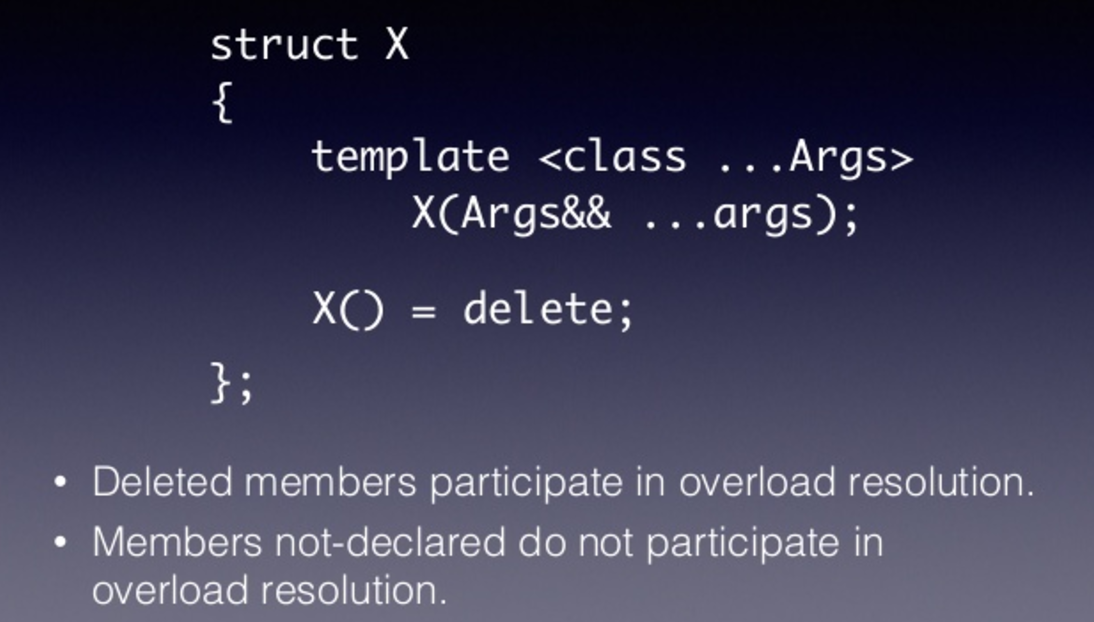
\includegraphics[scale=0.6]{pics/sm5.png} \newline

\end{itemize}

\subsubsection{Rules of implicitly declare }
\begin{itemize}
	\item The Default constructor, will not be implicitly generated if:
	
\begin{enumerate}
	\item you have explicitly declared any constructor.  Compiler doesn't create a default constructor if we write any constructor even if it is copy constructor.

	\item There is a member in your class that is not default-constructible (such as a reference, a const object, or a class with no or inaccessible default constructor)

	\item (C++11) you have explicitly told the compiler to not generate one using A() = delete;
\end{enumerate}

\item The copy constructor, will not be implicitly generated if:
\begin{enumerate}
	\item you have explicitly declared a copy constructor (for class X a constructor taking X, X\& or const X\&)
	
	\item there is a member in your class that is not copy-constructible (such as a class with no or inaccessible copy constructor)
	
	\item (C++11) you have explicitly told the compiler to not generate one using A(const A\&) = delete;
\end{enumerate}


\item The Copy Assignment Operator will not be implicitly generated if
\begin{enumerate}
\item you have explicitly declared a copy-assignment operator (for class X an operator = taking X, X\& or const X\&) )
\item there is a member in your class that is not assignable (such as a reference, a const object or a class with no or inaccessible assignment operator)
\item (C++11) you have explicitly told the compiler to not generate one using A\& operator=(const A\&) = delete;
\end{enumerate}


\item The Destructor will not be implicitly generated if
\begin{enumerate}
\item you have explicitly declared a destructor
\item (C++11) you have explicitly told the compiler to not generate one using ~A() = delete;
\end{enumerate}

\item The Move Constructor or Move Operator(C++11) will not be implicitly generated if
\begin{enumerate}
\item you have explicitly declared a move constructor or move assignment(for class X, a constructor taking X\&\&)
\item there is a member in your class that cannot be moved (have deleted, inaccessible, or ambiguous)
\item you have defined a copy assignment operator, copy constructor, destructor, or move assignment operator
\item you have explicitly told the compiler to not generate one using A(A\&\&) = delete;
\end{enumerate}


\item The Move Assignment Operator (C++11) will not be implicitly generated if
\begin{enumerate}
\item you have explicitly declared a move assignment operator (for class X, an operator = taking X\&\&)

\item you have defined a copy assignment operator, copy constructor, destructor, or move constructor.

\item you have explicitly told the compiler to not generate one using A\& operator=(A\&\&) = delete;
\end{enumerate}

\item  The justification is that declaring a copy operation (construction or assignment) indicates that the normal approach to copying an object(memberwise copy) isn't appropriate for the class, and compilers thinks that if memberwise copy isn't appropriate for the copy operations, memberwise move probably isn't appropriate for the move operations either.

\item The same idea as the previous item, declaring a move operation (construction or assignment) in a class causes compilers to disable the copy operations.

\item The two copy operations are independent: declaring one doesn't prevent compilers from generating the other. The two move operations are not independent. If you declare either, that prevents compilers from generating the other.

\item C++11 deprecates the automatic generation of copy operations for classes declaring copy operations or a destructor. This means that if you have code that depends on the generation of copy operations in classes declaring a destructor or one of the copy operations, you should consider upgrading these classes to eliminate the dependence. Provided the behavior of the compiler-generated functions is correct (i.e, if memberwise copying of the class's non-static data members is what you want), your job is easy, because C++11's "= default" lets you say that explicitly:

\item If you declared a destructor, implicitly defaulted copy member are deprecated.  \\

\begin{center}
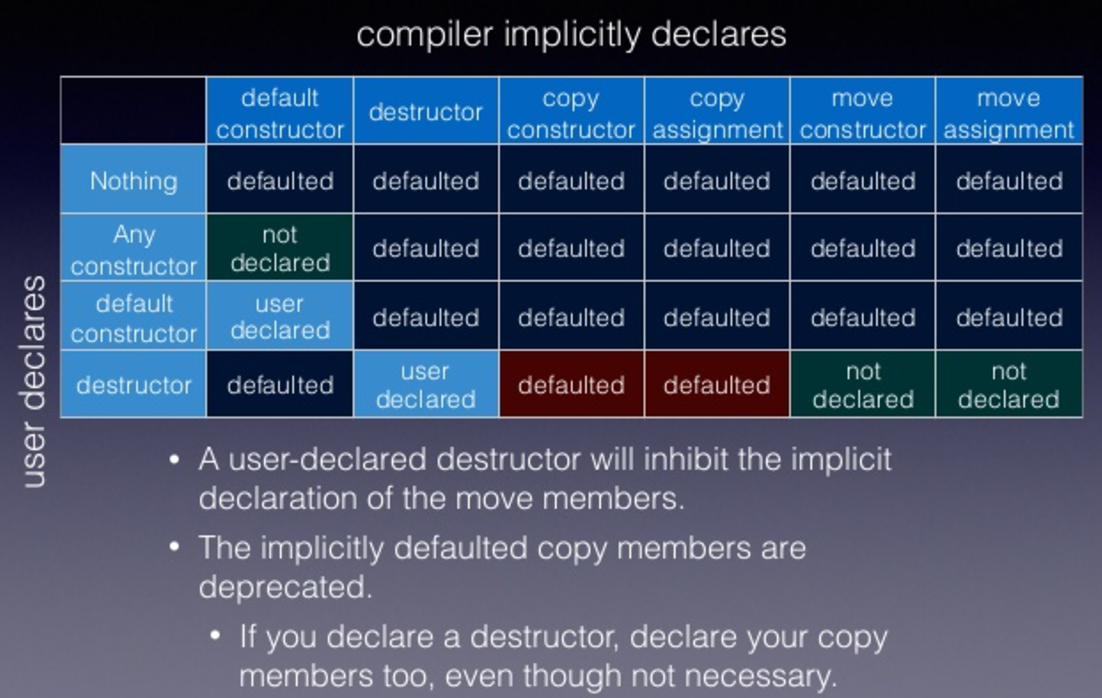
\includegraphics[scale=0.6]{pics/sm4.png} \newline
\end{center}

\item A summary can be seen below: \\
\begin{center}
	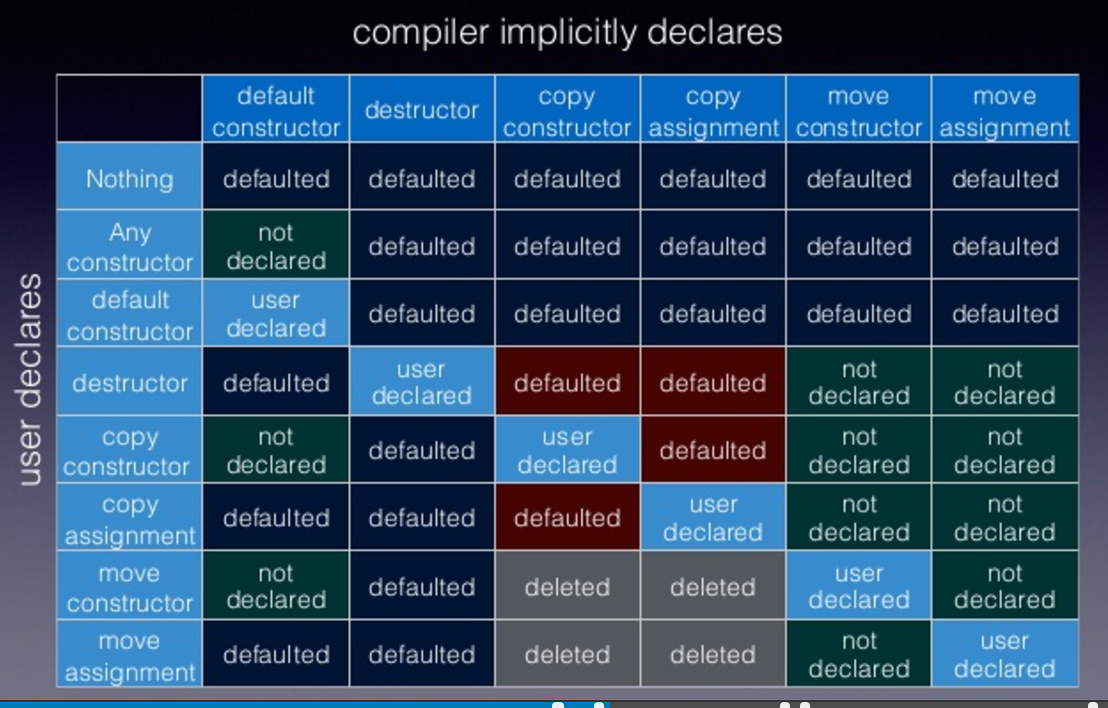
\includegraphics[scale=0.6]{pics/sm3.png} \newline
\end{center}

\end{itemize}

\subsection{Resource managment policy}
\begin{itemize}
    \item If a class only include value-like member, we usually don't need resource managment policy. In another word, 
we don't have to build any copy and move constructor, just use the compiler generate default one. That is the \textbf{Rule of zero}.
\begin{lstlisting}
class NoResource{
value-like member1; // such string s;
value-like member2; // such as int i;
\end{lstlisting}

    \item If a class includes reference-like member, things becomes a little complex. You need to consider Ownership or lifetime control. 

\begin{lstlisting}
class OneRef{
reference-like member1;
}
\end{lstlisting}

    \item If a class includes resource member, we can use \textbf{Four and half rule}, which will be introduced below:
\end{itemize}

\subsubsection{Rule of zero}
\begin{itemize}
    \item Rule of zero: If you can avoid defining default operations, do! It’s the simplest and gives the cleanest semantics. If all members have all the special functions, no further work is needed.
	
\begin{lstlisting}
struct Named_map {
public:
		// ... no default operations declared ...
private:
		string name;
		map<int, int> rep;
	};
\end{lstlisting}

	\item A variant of Rule of zero: As long as you can, stick to the Rule of Zero, but if you have to write at least one of the Big Five, default the rest. Why? detail can be google "The Rule of Zero in C++" in Fluent C++.
	 
\begin{lstlisting}
class X{
public:
	X(X const& other) = default;
	X& operator=(X const& other) = default;
	
	X(X&& other) = default;
	X& operator=(X&& other) = default;
	~X() { /* log something in the dtor */ }
};
\end{lstlisting}

    \item Any time you have resource, you can put it into the wrapper and change it into value-like memeber, in this way, we can follow Rule of zeor.

\begin{lstlisting}
class ZeroRule{
unique_ptr<Foo> p; //don't use Foo* p;
shared_ptr<Foo> p; //for shared ownership;
string s;  //don't use char* p;
vector<int> v; //don't use int* p;
array<int> a; //don't use int *p;
std::unique_ptr<void, decltype(&::FreeLibrary)> handle; //don't use HMODULE handle;
\end{lstlisting}

    \item Any time, if it's possible, you should consider to follow rule oe zero first. If there is not correct wrapper class, such as \texttt{unique\_ptr} to meet your requirement, or you want to manage your resource by you self, then you will follow rule of four and half. The rule of four uses "copy and swap idiom", so I will introduce the "copy and swap idiom" first, then jump to rule of four and half.

\end{itemize}

\subsubsection{copy and swap idiom}
\begin{itemize}
	\item Any class that manages a resource (a wrapper, like a smart pointer) needs to implement The Big Three. While the goals and implementation of the copy-constructor and destructor are straightforward, the copy-assignment operator is arguably the most nuanced and difficult. How should it be done? What pitfalls need to be avoided?
	
	\item The old implementation need  \textbf{1) avoid assignment self 2) return *this reference. }There are two problems, the first one is the old implementation is not strong exception safe. For example, when we copy the content1, an exception has been thrown. Under such context, original one has been damaged. The second problem is so many duplicated code. The assigment code has the same code with copy constructor.
\begin{lstlisting}[numbers=none]
class & class::operator=(class &a){
	if(this == &a)
	return *this;  //avoid assign by himself
    this.content1 = a.content1; //
    this.content2= a.content2; 
	return *this ; // return *this reference.
}	
\end{lstlisting}
	
	\item The copy-and-swap idiom is a better solution, and elegantly assists the assignment operator in achieving two things: \textbf{avoiding code duplication, and providing a strong exception guarantee.}  Conceptually, it works by using the copy-constructor's functionality to create a local copy of the data, then takes the copied data with a swap function, swapping the old data with the new data. The temporary copy then destructs, taking the old data with it. We are left with a copy of the new data. In order to use the copy-and-swap idiom, we need three things: a working copy-constructor, a working destructor (both are the basis of any wrapper, so should be complete anyway), and a swap function. The swap function can be a member function.
    \item A low effeicent implementation with swap. We should not use reference as function parameter. \textbf{No matter lvalue or rvalue, copy always happen inside assignment operator.}
\begin{lstlisting}[numbers=none]
dumb_array& operator=(const dumb_array& other){
	dumb_array temp(other);
	swap(*this, temp);
	return *this;
}	

dumb_array da;
da = f(); // use const & get the pvalue, // but inside the operator =, we copy. 
// we didn't use move, so it's low effeicient.	
\end{lstlisting}
	
	\item  A efficent way is to use value parameter. On a general note, a remarkably useful guideline is as follows: if you're going to make a copy of something in a function, let the compiler do it in the parameter list.
	
\begin{lstlisting}[numbers=none]
dumb_array& operator=(dumb_array other){
	other.swap(*this); 
	return *this;
}	

dumb_array da;
da = f(); // use move directly. high effeicient.
\end{lstlisting}
	

\item The full code is here:
\begin{lstlisting}[numbers=none]
class dumb_array{
	dumb_array(const dumb_array& other)
		: mSize(other.mSize),
			mArray(mSize ? new int[mSize] : nullptr){
	std::copy(other.mArray, other.mArray + mSize, mArray);
	}

	dumb_array(dumb_array&& other) noexcept{
		mSize = other.size;
		mArray = other.mArray;
		other.mArray = nullptr;
	}

	void swap(dump_array& rhs) noexcept{
		using std::swap;
		swap(msize, rsh.msize);
		swap(mArray, rsh.mArray);
	}
	
	dumb_array& operator=(dumb_array other) noexcept{
		other.swap(*this); 
		return *this;
	}

private:
	std::size_t mSize;
	int* mArray;
};

void swap(dumb_array& first, dumb_array& second) {
	first.swap(second);
}
\end{lstlisting}
\begin{description}
    \item[Soure code] Why do we need member swap, because it can visit private member of class.

    \item[Sourc code] If \texttt{dump\_array} has it's own namespace, then put swap non-member swap function into the same namespace.In this way, client can use ADL find this version and pick it up.

\begin{lstlisting}
namespace_dr::dumb_array dr1;
namespace_dr::dumb_array dr2;
swap(dr1, dr2); // will go to namespace_dr to find the correct swap function.
\end{lstlisting}

    \item [Source code] If \texttt{dump\_array} is in global space, you can put swap into the std namesapce and make it specilaization.
\begin{lstlisting}
namesapce std{
template<> 
void swap<dump_array>{dump_array& first, dump_array& seconde){
	first.swap(second);
}

//clients code should be like this
using std::swap
swap(dr1, dr2); 
\end{lstlisting}

\end{description}

\item Summary:
\begin{enumerate}
	\item Build swap member function, use global swap to exchange class member and label it noexcept.

	\item Build global non-member swap function, to hide global swap name to exchange two \texttt{dumb\_array}. Because global default swap need deep copy and low efficient. If your class has its own namespace, put non-member swap into this namespace, then ADL will find it. If your class doesn't have its namesapce, put non-member swap into the std namespace as template specification. 
	\item Use swap member function to implement assignment operator, the function parameter is value, and label it noexcept. 
	\item Build move member funciton, and label it noexcept. \textbf{That is very import, when we use vector<dump\_array>, when vector need expand its size, it will use move if move is noexcept, if move is not noexcept, it will use copy which deep copy happens. }
\end{enumerate}
\end{itemize}
	
\subsubsection{Rule of four and half}
\begin{itemize}
		\item Before C++11, we don't have move semantics. We just need to follow Rule of three: If a class requires a user-defined destructor, a user-defined copy constructor, or a user-defined copy assignment operator, it almost certainly requires all three.
	
	\item After C++11, we introduced move semantic, so rule of three become rule of five. Add move constructor and move assignment.
	
	\item With help "copy and swap idiom", the rule of five becomes to the Rule of The Big Four (and a half), which states that if you implement one of
	\begin{enumerate}
		\item The copy constructor
		\item The assignment operator.\textbf{Don't need move assignment, in assignment operator, we pass only one kind of type--value.} 
		\item The move constructor
		\item The destructor
		\item The swap function(that is half)
	\end{enumerate}
    Once we have swap functions, we can use it to implement assignment operator, can move constructor. Here I will use the previous \texttt{dump\_array} as example. 
\begin{lstlisting}[numbers=none]
dumb_array(dumb_array&& other):dumb_array{} noexcept{
    *this.swap(other);
}

dumb_array& operator=(dumb_array other) noexcept{
    other.swap(*this); 
    return *this;
}
\end{lstlisting}
	
\end{itemize}

\subsubsection{Summary}
\begin{itemize}
    \item For non-resource class follow zero rule, for wrapping-resource class, follow four and half rule. Don't use big three rule, it's deprecated after C++ 11.

    \item You can use \texttt{=default} and \texttt{=delete} to explicitly declare some special member functions. For example, if you define destructor for log purpose, it will disable copy constructor generation, at this time, you can add \texttt{Foo Foo(cont Foo\& rhs)=default}.
        
    \item The common use resource management policies are below:

\begin{enumerate}
    \item Objects that can be both moved and copied
        \item Objects for which it makes sense to copy but not move
        \item Objects for which it makes sense to move but not copy
        \item Objects which should neither be moved not copied.
\end{enumerate}

	\item Besides these famous idiom, you can customize your own class management policy. Different policy will make the class has different behavioral, then represents the piratical application semantic the best. 
	
	\begin{enumerate}
		\item Use the compiler-provided versions of these functions. In other words, you're not doing any resource management in the class.
		
		\item Write your own move functions, but don't support copying.(\texttt{std::unique\_ptr})
		
		\item Disable copying and move semantics for the class, because it doesn't make sense to allow it.
		
		\item For \texttt{std::unary\_function}, it's base class, but it's just trait class.(extract type information from a function). You can declare its destructor as protect and non virtual. Then your client can't use below code:
\begin{lstlisting}[numbers=none]
class Base {
protected:
	~Base(){
		cout<<"Base::Destructor\n";
	}
};

Base *base_ptr = new Base{};
delete base_ptr; //compiler barks here.
\end{lstlisting}
	\end{enumerate}

\end{itemize}

\subsection{operator overload}
\begin{itemize}
	\item \textbf{Never overload \&\&, || and comma in C++.  Just remember it!}
	
	\item You can declare operator as member function. if it's not member function, declare it as a friend function if it need to visit private member variable. If you want to overload + operator, and support time t; 3+t;   You need to define a friend function. In order to improve a \texttt{t+3} efficiency, you also can define a member function time \texttt{operator+(int i)} member function.
\begin{lstlisting}[frame=single, language=c++]
time operator+(const time &t) const;
friend time operator+(int,  const time &t)
time operator+(int i)
\end{lstlisting}
\begin{description}
	\item[Line 1:] member function. for \texttt{t = t1+t2}. \texttt{t = t1+t2} will changed to:  \texttt{t1.operator+(t2);}  The last const make the \texttt{t1} to invoke this operator doesn't change the value in this class. 
	
	\item[Line 2:] nonmember friend function. for \texttt{3+t}.
	
	\item[Line 3:] member function, for \texttt{t+3}, to avoid implicit conversion from 3 to obj.
\end{description}
	
	\item \textbf{For Binary Arithmetic Operators + - *, implement Compound Assignment Operators += -= *= first, then use these Compound Assignment operators}
	
	\item \textbf{Use += implement operator +}. It's very good design. It provides two advantages. 1) give another function, 2) avoid code duplication. Compound assignment operators should be overloaded as member functions, as they change the left-hand operand. Like all other operators (except basic assignment), compound assignment operators must be explicitly defined. 
\begin{lstlisting}[numbers=none]
Vector2D& Vector2D::operator+=(const Vector2D& right){
	this->x += right.x;
	this->y += right.y;
	return *this;
}
\end{lstlisting}
	
\begin{lstlisting}[numbers=none]
Foo operator+(const Foo& lhs, const Foo& rhs){
	Foo result = lhs;
	result += rhs;
	return result;
}
\end{lstlisting}
	
	\item Why \verb=<<= need to be friend? You need to consider:  Because you need to write cout\verb=<<= obj. If you declare \verb=<<= as a member operator, you have to write obj\verb=<<=cout; it looks weird.
	
	\item Assignment operator overload returns a non-const reference. Don't return const reference, somebody said that it can avoid (x=y)=z. But in fact, it's not a normal way to write such code. In STL string, assignment operator just return reference. It give you a clue, \textbf{any time you have questions about interface design, you can see the STL library.}
\begin{lstlisting}[numbers=none]
class A & operator=(const class A& rhs){	
	//Do some things other
	return *this;
}
\end{lstlisting}
	
\end{itemize}


\section{Object oriented}

\subsection{Inheritance}
\subsubsection{Polymorphism by inheritance}

\begin{itemize}
	\item polymorphism is a powerful design mechanism that allows for the encapsulation of related types behind an abstract public interface, The cost is an additional level of indirection, both in terms of memory acquisition and type resolution. This style of programming is called object-oriented. Only reference and pointer support polymorphism, see source code below:

\begin{lstlisting}[numbers=none]
class A{
public:
	virtual void fun(){ cout<<"A";}
};
	
class B: public A{
public:
	void fun(){cout<<"B";}
	int m_b = 100;
};
\end{lstlisting}

	\item Base pointer can't access class member in derived class directly.
	
\begin{lstlisting}
B b;
A* pa = &b;
cout<<b.m_b;    //OK,You can access class member by object directly.
//cout<<pa->m_b;   //ERROR 
//cout<<(*pa).m_b; //ERROR
cout<<static_cast<B*>(pa)->m_b; //OK
\end{lstlisting}
\begin{description}
	\item[Line 4:] Error, it doesn't work. Pointer has type. The pointer type alter the interpretation of the size and composition of the memory. Pointer type is A, so the size of memory which pointer address is sizeof(A), that's why you can't see the \texttt{m\_b}.at all.
	\item[Line 6:] OK, when you change the pointer type from A to B, then the memory which pointer address is \texttt{sizeof(B)}, interpretation also support \texttt{->m\_b} 
\end{description}

\item Base object doesn't support polymorphism.
\begin{lstlisting}
B b;
A a = b;
a.fun(); //output A
\end{lstlisting}
\begin{description}
	\item[Line 2:] When a base class object is directly initialized or assigned with a derived class object, the derived object is sliced to fit into the available memory resources of the base type. There is nothing of the derived type remaining. 
	\item[Line 3:] Polymorphism is not present, and an observant compiler can resolve an invocation of a virtual function through the object at compile time, thus by-passing the virtual mechanism.
\end{description}

\item A pointer or a reference support polymorphism because in derived class, we build virtual table, (adding indirect level.)
\begin{lstlisting}
A& ra = b;
ra.fun(); //output B
A* pa = &b;
pa->fun(); //output B
(*pa).fun(); //output B
		
A* pa1 = new B; //virtual table content has not changed.
(*pa1).fun(); //output B

A a = b; //when you copy,slice happens here, virtual table content changed. 
a.fun() //output A here
}
\end{lstlisting}

\end{itemize}

\subsection{Member functions in inheritance}

\subsubsection{constructor in inheritance}
\begin{itemize}
	\item  \textbf{Subclass constructor will always call base class constructor.} Idea behind this rules is \textbf{Do best to make sure a obj can be initialized properly}. Constructor should NOT be virtual. If subclass doesn't define any constructor, compiler will implicitly define a default ctor, and this ctor will call base class default ctor.If subclass has a constructor, but it doesn't explicitly call base specify ctor, ctor of subclass will call base default ctor.(without any parameter.) If base ctor only has specify ctor, no default ctor, produce compiler error. If you want explicitly call base specify constructor, use initialization list syntax.	
\begin{lstlisting}[frame=single, language=c++]
class base{
	public:
	base();  //default constructor
	base(int b); //specify constructor
	private:
	int b;
};
	
class subclass: public base{
	subclass();  //default constructor
	subclass(int s, int b); // specify ctor1
	subclass(int s);     //specify ctor2
	int s;
};
	
subclass::subclass(int s, int b): base(b){
	m_s = s;
}
//////////////////////////////////////////
subclass sc1(2,3); //call specify constructor, then explicit call base specify constructor.

subclass sc2(2);  // implicit call base default constructor
subclass sc3;   // implicit call base default constructor

}
\end{lstlisting}
\begin{description}
	\item[Line 22:] if base has not default constructor, \texttt{sc2} and \texttt{sc3} will produce error.
\end{description}

	\item If you don't use  explicitly initialization list syntax to call base specify constructor, You will get uninitialized value or you can't initialize base member, Neither are good.
\begin{lstlisting}[frame=single, language=c++]
DeriveClass::DeriveClass(int base_a, b){
	Derive_b = b
}	

DeriveClass::DeriveClass(int base_a, b) {
	base_a = a  //It can be thought as a bad design.
	Derive_b = b
}
\end{lstlisting}
\begin{description}
	\item[Line 1:] it will call \texttt{base\_class} default constructor. in this case, \texttt{base\_a} is not assigned at all.
	\item[Line 6:] You can't  access private base member data. \texttt{base\_a} need to be public member data.
\end{description}

\end{itemize}


\subsubsection{destructor in inheritance}
\begin{itemize}
	\item For destructor:
	\begin{enumerate}
		\item If a base class has a destructor, but sub class doesn't have,  compiler will produce an implicit default destructor, and this implicit default destructor will call base class destructor.
		
		\item If you define a subclass destructor, It will call base destructor automatically, you don't need to call it explicitly.
		
		\item The question is, How can you make sure you sub class destructor will be called if you use a base class pointer or reference, answer is below:
	\end{enumerate}
	
	\item Don't call base destructor explicitly, It will called automatically in the reverse order of construction.  And you should give a base destructor a definition, Or linker will report error it even you don't call it in your source code.
	
	\item \textbf{Make base class destructor public and virtual} (polymorphic deletion by base class pointer or reference), or protect and non-virtual, base classes need not always allow polymorphic deletion. For example, consider class templates such as \texttt{std::unary\_function}. This time, you should make destructor protected and non-virtual.
\begin{lstlisting}[numbers=none]
template <class Arg, class Result>
struct unary_function{
	typedef Arg    argument_type;
	typedef Result result_type;
};
	
void f( std::unary_function* f ){
	delete f; // error, illegal
}
\end{lstlisting}
\begin{description}
	\item[Line 8:] Make destructor protected and non-virtual, then this line will compile with failure, it's good design. 
\end{description}
	
	\item Never throw exception from destructor, if exception A is thrown, then stack-unwindling, when a obj is destructed, then destructor is called, when another exception B is thrown by the destructor, application will call terminate function immediately.  If you have exception, catch it inside of the destructor.
	
\end{itemize}



\subsubsection{copy constructor in inheritance}

\begin{itemize}
	\item copy constructor(assignment constructor) in inheritance sometimes causes \textbf{slicing problem}.   Below four are all SLICING.  number 4 and number 5 is not very obvious. They all call base class constructor.  No matter what you input a reference to a derived class or not.
\begin{lstlisting}[numbers=none]
class Base{};
class Derived1 : Base{};
class Derived2 : Base{};
Derived1 d1;
Derived1 d2;
/////////////////////
Base b = d1; //1)
	
Fun(Base b);
Fun(d1);  //2)
	
Base& Bref = d1;
Fun(Bref) //3)
	
Base* bp = new Base(Bref); //4) call base copy constructor
	
Base* bp1 = new Derived1();  //5) sibling slicing
base* bp2 = new Derived2();
*bp1 = *bp2;  // bp1 just copy Base part in Derived2.
//so bp1 now is MIXTURE of d1 and d2.
\end{lstlisting}

%	\item What does a typical user defined move constructor do?
%\begin{lstlisting}[numbers=none]
%class Child : public Base{
%	Member m_;
%	Child(Child&& x): Base(std::move(x)), m_(std::move(x.m_)){
%		x.set_to_resourceless_state();
%	}
%}
%\end{lstlisting}
	
	
\item Think a problem as below: how to make deep copy and avoid slicing in base class copy constructor?
\begin{lstlisting}[numbers=none]
class Base{};
class Derived1 : Base{};
class Derived2 : Base{};
Derived d1;
Derived d2;
	
Base* Copy(Base& Bref){
	//How to avoid slicing and make deep copy.
}
	
Base& Bref = d1
Base* d1p = Copy(Bref)

Base& Bref = d2
Base* d2p = Copy(Bref)
	\end{lstlisting}
	
\item Continue- Think this problem: error method
\begin{lstlisting}[numbers=none]
Base* Copy(Base& Bref){
	Base* p = new Base(Bref)
	//Slicing happen. bad
}
\end{lstlisting}
	\item Continue- Think this problem: TypeID method.
\begin{lstlisting}[numbers=none]
Base* Copy(Base& Bref){
	int typeid;
}
\end{lstlisting}
\begin{description}
	\item[Line 1:] Use \texttt{type\_id} and \texttt{dynamic\_cast}. involve a lot of if and switch about type. anytime if you use \texttt{dynamic\_cast} and \texttt{if}, you can think about using virtual function instead.
\end{description}
	
\item Continue- Think this problem: Virtual Clone method.
	A function's return type is never considered part of its signature. You can override a member function with any return type as long as the return type could be used wherever the base class return type could be used.
\begin{lstlisting}[numbers=none]
class Base{
	virutal Base* Clone() = 0;
};
	
class Derived1 : Base{
	virutal Derived1* Clone(){return new Derived1(*this);}
}
	
Base* Copy(Base& Bref){
Base* p = Bref.Clone();
}
\end{lstlisting}
	
	\item Continue- Think this problem: Change Design. Base is concrete class,  More Effective C++ Item 33 said"Making Non-leaf class abstract. So maybe you can change the inheritance system.
	
	\item \textbf{Assignment operator and copy constructor in inheritance summary:}

	\begin{enumerate}
		\item Default Assignment  operator and  copy constructor in derived class which are implicitly produced by compiler will call default base assignment operator and  copy constructor.
		
		\item If derived class has no new operation. Don't need to define derived class Assignment  operator and  copy constructor, implicit one will call base one automatically.
		
		\item \textbf{If derived class has new operation. You have to define derived class Assignment  operator and  copy constructor, it will not invoke assignment  operator and  copy constructor in base class any more}.  Inside, manually invoke base class Assignment operator and copy constructor. Detail can be found in C++ primer p760. Syntax looks like below: see effective C++ Item 16.
		
		\item For copy constructor, just initialization list syntax. For assignment operator, use two different methods depends on if base class declare its own assignment operator(). Source code is below:
		
\begin{lstlisting}[frame=single, language=c++]
DerivedClass::DerivedClass(const DerivedClass &dc): \
	BaseClass(dc){...}  //init list syntax here.
		
DerivedClass & DerivedClass::operator=(const DerivedClass &dc){
    BaseClass::operator=(dc);
    ( (BaseClass&) *this ) = dc
    ( (BaseClass) *this ) = dc // this will call baseclass copy constructor.
}
\end{lstlisting}

\begin{description}
	\item[Line 5:] If base class declare explicitly operator, we can call it explicitly.
	\item[Line 6:] Base class no explicitly operator, change \texttt{*this} to \texttt{BaseClass} reference, if you change to \texttt{BaseClass}, It will call copy constructor.
\end{description}
		
	\end{enumerate}

%	\item There are three articles, you should read them together.\\
%\\
%https://herbsutter.com/2013/05/09/gotw-1-solution/
%\\
%https://stackoverflow.com/questions/21825933/any-difference-between-copy-list-initialization-and-traditional-copy-initializat
%\\
%https://stackoverflow.com/questions/1051379/is-there-a-difference-between-copy-initialization-and-direct-initialization

\end{itemize}

\subsection{virtual function and override}

\begin{itemize}
	
	\item Only virtual function come into vtbl. Friend can't be virtual function, because it's not even a member of class. When a method is declared virtual in a base class, it is automatically virtual in the derived class, but it is a good idea to explicitly declare it by using the keyword virtual in the derived class declarations too.
	
	\item \textbf{Almost all the base class has virtual function, if a class doesn't contain a virtual function, It is an indication that it is not meant to be used as a base class.} Some base classes are just for injecting some type, such as unary\_function 
	
	\item Don't rewrite non-virtual base member function.
	
	\item For overriding to occur, several requirements must be met:
	\begin{enumerate}
		\item The base class function must be virtual.
		\item The base and derived function names must be identical (except in the case of
		destructor).
		\item The parameter types of the base and derived functions must be identical.
		\item The constness of the base and derived functions must be identical.
		\item The return types and exception specifications of the base and derived functions
		must be compatible.
		\item To these constraints, which were also part of C++98, C++11 adds one more: The functions' reference qualifiers must be identical.
	\end{enumerate}
	\item reference qualifier explain:
\begin{lstlisting}
class Widget {
public:
	void doWork() &;  //This doWork applies only when *this is an lvalue.
	void doWork() &&; //This doWork applies only when *this is an rvalue.
}; 
	
	Widget makeWidget(); // factory function (returns rvalue)
	Widget w; // normal object (an lvalue)
	
	w.doWork();  //call Widget::doWork &
	makeWidget().doWork();  //call Widget::doWork &&
	
\end{lstlisting}

	
\item Any small error will not real override base virtual function. But creating a new virtual method with a different signature. such as examples below.

\begin{lstlisting}[numbers=none]
class Base {
public:
	virtual void mf1() const;
	virtual void mf2(int x);
	virtual void mf3() &;
	void mf4() const;
};

class Derived: public Base {
public:
	virtual void mf1();
	virtual void mf2(unsigned int x);
	virtual void mf3() &&;
	void mf4() const;
};
\end{lstlisting}
	
	\item Override specifier should be used in derived class member function used to check if they are match with member function in base class. It can overcome all the implicit non-override problem in the previous source code.
\begin{lstlisting}[numbers=none]
struct A{
	virtual void foo();
	void bar();
	virtual void goo(const int);
};
	
struct B : A{
	void foo() override; // OK: B::foo overrides A::foo.
	void bar() override; // Error: A::bar is not virtual.
	void goo(int) override; //Error; differenet signature. 
}
\end{lstlisting}
	
    \item Use final in Base class, to stop sub-class override.
\begin{lstlisting}[numbers=none]
class Base{
	virtual void method1() final;
}
\end{lstlisting}
	
\end{itemize}

\section{Classes relationship}

\subsection{structure semantic}

\subsubsection{Relationship}

\begin{itemize}
	\item OOP has five relationships:
	\begin{description}
		\item[Composition ] exists when a member of a class has a \textbf{part-of} relationship with the class. In a composition relationship, the class manages the existence of the members. To qualify as a composition, an object and a part must have the following relationship:
		\begin{enumerate}
			\item The part (member) is part of the object (class)
			\item The part (member) can only belong to one object (class) at a time
			\item The part (member) has its existence managed by the object (class)
			\item The part (member) does not know about the existence of the object (class)
		\end{enumerate}
	More descriptions: 
	\begin{enumerate}
		\item Compositions are typically implemented via normal member variables, or by pointers where the class manages all the memory allocation and deallocation. If you can implement a class as a composition, you should implement a class as a composition.
		\item  Ownership, same life time,  not change in the middle. Such as person and head.
	\end{enumerate}
	
	
	\item[Aggregations ] exists when a class has a \textbf{has-a} relationship with the member. In an aggregation relationship, the class does not manage the existence of the members. To qualify as an aggregation, an object and its parts must have the following relationship:
	
	\begin{enumerate}
		\item The part (member) is part of the object (class)
		\item The part (member) can belong to more than one object (class) at a time
		\item The part (member) does not have its existence managed by the object (class)
		\item The part (member) does not know about the existence of the object (class)
	\end{enumerate}
	More descriptions: 
	\begin{enumerate}
		\item Aggregations are typically implemented via pointer or reference.
		\item Ownership, maybe same life time, may change in the middle,  Container and pointer(same life time, changeable). Airport and airplane and department and teacher.
        \item Aggregations are typically implemented via pointer or reference.
	\end{enumerate}
	
	\item[Associations  ] are a looser type of relationship, where the class \textbf{uses-a} object. To qualify as an association, an object and an associated object must have the following relationship:
	\begin{enumerate}
		\item The associated object (member) is otherwise unrelated to the object (class)
		\item The associated object (member) can belong to more than one object (class) at a time
		\item The associated object (member) does not have its existence managed by the object (class)
		\item The associated object (member) may or may not know about the existence of the object (class)
	\end{enumerate}
	More descriptions:
	\begin{enumerate}
		\item Associations may be implemented via pointer or reference, or by a more indirect means (such as holding the index or key of the associated object). No Ownership, different life time,
		
		\item People and toothbrush(same life time, changeable) Teacher and student( not same life time, changeable), person and father(Not Nullity), person and wife( Nullity)
	\end{enumerate}

	\item[Dependency ] exists when a member of a class has a part-of relationship with the class. In a composition relationship, the class manages the existence of the members. To qualify as a composition, an object and a part must have the following relationship:
	
	More descriptions:
	\begin{enumerate}
		\item No Ownership, Not Includes as a member, person and friend.
		
		\item \textbf{Dependency definition: If class X's member function argument is class Y, X is dependency of Y.}
		
		\item Dependency definition extension: For a class X, all functions, including free functions, that both "Mention" X and "supplied with" X are logically part of X, because they form part of the interface of X. Supplied with means that they appear in the same header file.
	\end{enumerate}

	\item [Inheritance ] Aggregations are typically implemented via pointer or reference.
\begin{enumerate}
	\item Main disadvantage: Tightly coupled, fragile, prone to be abused by developers
\end{enumerate}

	\item [Summary:] \textbf{Composition is specific aggregation, and aggregation is specific associate.}
	\end{description}

\begin{center}
	\begin{tabular}{|p{0.25\textwidth}|p{0.12\textwidth}|p{0.12\textwidth}|p{0.15\textwidth}|p{0.15\textwidth}|}
		\tophline 
		 & Composition  & Aggregation  & association & Dependency \\ 
		\tophline 
		Relationship type& Whole/part  & Whole/part  & otherwise unrelated  & otherwise unrelated  \\ 
		\tophline 
		Members can belongs to multi classes& no  & yes & yes & yes  \\ 
		\tophline 
		member existence managed by class& Yes & no & no   & no \\ 
		\tophline 
		Directionality & uni  & uni & uni or bidirectional & uni  \\ 
		\tophline 
		relationship verb& part-of & has-a & uses-a & depends-on 
		\bottomhline 
	\end{tabular}
\end{center}

	\item \textbf{Composition is specific aggregation, and aggregation is specific associate.}

	\item For Aggregation, It is not a very clearly defined concept and in my opinion it causes more confusion than it is worth. For example, toothbrush and people can be thought as aggregate from \textbf{structural relationship perspective}, at the same time, toothbrush and people can not be thought as association relationship \textbf{semantic relationship perspective}. So recent we intend to ignore aggregation OOP relationship. Composition and Association are quite enough.  
	
	\item We can delete aggregation relationship. In the future, we can only use association. From \textbf{implementation} perspective,  we can implement divid association into shallow copy and deep copy. 
	
	\begin{description}

		\item[Association-shallow copy:] Foo has a pointer to Bar object as a data member.
		\item[Association-deep copy:] Foo has a pointer to Bar object and data of Bar is deep copied in that pointer.
		\item[Composition:] Foo has a Bar object as data member.
	\end{description}

	\item We can not map relationship in real word into C++ 100\% accurate. C++ is programming language which has its own syntax and semantic understand. Just like we can not inherit ellipse from circle in C++, but we can do this in real word. So we should not treat all the above relationships too pedantically!

    \item In previous five relationships, inheritance is easy to understand, but is abused the most. I will introduce more deep thought about inheritance. 
	
\end{itemize}

\subsection{Go deeper into inheritance}

\subsubsection{Basic syntactic knowledge}
\begin{itemize}

	\item Some basic syntactic knowledge:
	\begin{enumerate}
		\item No source code, just header and lib, you also can use inheritance in C++ language.
		
		\item Pure virtual class can't be instance, it just a abstract interface, it's agreement between your class and class user(client).
\begin{lstlisting}[numbers=none]
class Shape{
	virtual draw() = 0 
}	//you have to redefine it in your child class
			
class Circle: public Shape{
	...
}
\end{lstlisting}
		
		\item Both reference and pointer support polymorphism.
	\end{enumerate}
	
	\item 	There are three kinds of inheritances. Code and example and explanation:
\begin{lstlisting}[frame=single, language=c++]
class B                    { /*...*/ };
class D_priv : private   B { /*...*/ };
class D_prot : protected B { /*...*/ };
class D_publ : public    B { /*...*/ };
\end{lstlisting}
	
	\begin{enumerate}
		\item None of the derived classes can access anything that is private in B.
		
		\item In D\_priv, the public and protected parts of B are private.
		
		\item In D\_prot, the public and protected parts of B are protected. Protect used in three generation inheritance. By protected Inheritance, grandfather member become protected member in father, so Grandson can still use grandfather's members.
		
		\item In D\_publ, the public parts of  B are public and the protected parts of B are protected (D\_publ is-a-kind-of-a B).
		
	\end{enumerate}

	\item To make a public member of B public in D\_priv or D\_prot, state the name of the member with a B:: prefix. E.g., to make member \texttt{B::f(int,float)} public in D\_prot, you would say:
\begin{lstlisting}[numbers=none]
class D_prot : protected B {
public:
	using B::f;  // Note: Not using B::f(int,float)
};
\end{lstlisting}
\end{itemize}

\subsubsection{private inheritance}
\begin{itemize}
    \item If you want to reuse string code in class student(also means \textbf{has-a} relationship, student has a string name) you have two options, The first is composition,  the second is private inheritance. See below:
\begin{lstlisting}[numbers=none]
class Student{ // 1) use composition.
	int getNameLen();
private:
	string m_name;
	vector<double> score;
};

int Student::getNameLen(){
	return m_name.length();
}
\end{lstlisting}

\item In short, composite uses object names to invoke a method, whereas private Inheritance uses the class name and scope resolution operator instead. If you need the base class itself, use a type case \texttt{(const string\&) * this}; detail can be seen in C++ primer, P800
\begin{lstlisting}[numbers=none]
class Student: private string, private std::vector<double>{
	int getNameLen();
	// We don't need private member data any more
}

int Student::getNameLen(){
	return string::length();
	//use class name and scope-resolution operator
}

const string& Student::getName(){
	return (const string&) *this;
}
\end{lstlisting}
\end{itemize}

\subsubsection{"Is-A" relationship}

\begin{itemize}
	\item Inheritance has three level knowledge.
	\begin{enumerate}
		\item The basic design knowledge, manager is a person, apple is a fruit, and bla bla bla.
		
		\item The basic  pure virtual, virtual, and non virtual syntax knowledge.
		
		\item \textbf{Isolate change between Client and Implement}. That is the highest level in design pattern. How to understand interface? Client<->Interface<->Implement. through Interface, you keep all the change happen in implementation side, not affect Client at all.
	\end{enumerate}
	
	\item \textbf{Public inheritance is substitutability, not to reuse, but to be reused. } For example, client use class A, and class B inherit class A.  I don't think class B reuse something in class A. we should think that class B could be used by client too, just like client use class A.
	
	\item  A common mistake is inheriting from classes that were not designed to be base class. For example, you want to customize some current class, you have string class, but you want to change some behavior of string. So you write: \texttt{class myString : public string}. But it violate LSP( Liskov Substitution Principle): \textbf{Functions That use pointers or references to base classes must be able to use objects of derived classes without knowing it. }
	\begin{enumerate}
		\item client use string class through base class pointer or reference
		\item base class has virtual function.
		\item derived class redefine base class virtual function.
	\end{enumerate}
	
	\item See previous three points: all requirement are not satisfied. Clients most times use string by value directly, string doesn't has any virtual function, it's a value class, and you didn't design before hand.
	
\item If you want to change find function, You don't need inherit,  Just write non-member function and pass a string object.
\begin{lstlisting}[numbers=none]
myFind(const string& str){
	//you custimized behavior.
}
// use myFind(str) and myStr.find()
//I think only difference is syntax.
\end{lstlisting}
	
    \item Even you have specific state, you also can use composition to avoid inheritance.

\begin{lstlisting}[numbers=none]
class MyString{
	size_t length(){return str.length}
	//just need to write forward function here;
	
	myFind(){
		//You customized behavior.
	}
	
	std::string str;
}
\end{lstlisting}
	
	\item \textbf{Another mistake is public inheritance is work-like-a, not is-a.} For example, circle is a eclipse, and square is a rectangle, but in oop, you can't make circle inherit from eclipse, because, eclipse has two centers.  you can't make square inherit from rectangle, because setWidth is not work as the same as in rectangle, (setWidth in square will change height at the same time.) It break LSP.  A solution is make an abstract base class(ABC) then make circle and ellipse inherit from ABC
	
	\item Previous example also explain, when you design a class, it doesn't need to be a practical object, such as animal, car, people, etc.  It can be abstract conception.  (So design pattern is so important conception).
	
	\item Composite VS Inheritance:
	\begin{enumerate}
		\item Does TypeB want to expose the complete interface (all public methods no less) of TypeA such that TypeB can be used where TypeA is expected? Indicates Inheritance. e.g. A Cessna biplane will expose the complete interface of an airplane, if not more. So that makes it fit to derive from Airplane.
		
		\item Does TypeB only want only some/part of the behavior exposed by TypeA? Indicates need for Composition. In this case, it makes sense to extract it out as an interface / class / both and make it a member of both classes.
		
		\item Inheritance must pass Liskov Substitution Principle. Previous example about ellipse and circle fail this test. because ellipse has setLongAxis() and setShortAxis(), but circle doesn't have them at all.
	\end{enumerate}

    \item There is a very good article: it explain the ellipse and circle debate in C++ community. \verb=https://isocpp.org/wiki/faq/proper-inheritance=. There are two important points:

        \begin{enumerate}
            \item \textbf{The biggest difference is to change "is-a" into "is-substitutable". }

            \item substitutable is defined by "contract". If the base class has a method void \texttt{insert(const Foo\& x)}, the \textbf{contract} of that method includes the signature (meaning the name insert and the parameter \texttt{const Foo\&}), but goes well beyond that to include the method’s \textbf{advertised preconditions and postconditions}. 

            \item For ellipse and circle dillema, You can 1)weak the base class promises, or 2)Strengthen child class promises. 3) Drop the inheritance relationship. 

            \item Even you drop inheritance relationship, in modern C++ age, you can also use lambda or closure to reach some kind of dynamic behaviour in the run time. \textbf{That is mainstream method in the future.}. With \texttt{std::function}, maybe we don't need any behaviour design pattern in the 23 design patterns. I hope that it will become true.:)
        \end{enumerate}

\end{itemize}

\subsection{"Has-A" relationship}
\begin{itemize}
	\item You can use \textbf{1)private inheritance, 2)composition, 3)template} three methods to describe has-a relationship.
	
	\item Private and protect inheritances are used to implement has-a relationship. 

	\item \textbf{Prefer composition, use private inheritance when you have to.} Reusing by private inheritance is weird in syntax and difficult to understand. One exception is you have to access string or vector<T> protect member function, at this time, you MUST use private inheritance.
	
	\item By now, I want to not only reuse class A, I also want to make a class adaptable. or make it possible to select different algorithms from the outside.  An example is  to replace brakes of a car (at runtime), There are three options.
	\begin{enumerate}
		\item Version 1: Abstract base class, In fact, consider \textbf{same life time and composition relationship},  Using Brake obj directly is better. But you want to have runtime polymorphism at the same time, So have to use pointer or reference. Here you can also use smart pointer\texttt{(uniqu\_ptr)}.
\begin{lstlisting}[numbers=none]
class Brake {
	public: virtual void stopCar() = 0;
};
		
class BrakeWithABS : public Brake {
public: void stopCar() { ... }
};
		
class Car {
	Brake* _brake;
public:
Car(Brake* brake) : _brake(brake) { brake->stopCar(); }
};
\end{lstlisting}
		
		\item Version 2a: Template
		
\begin{lstlisting}[numbers=none]
template<class Brake>
class Car {
		Brake brake;
public:
		Car(){ brake.stopCar(); }
};
		
\end{lstlisting}
		\item Version 2b: Template and private inheritance
\begin{lstlisting}[numbers=none]
template<class Brake>
class Car : private Brake {
		using Brake::stopCar;
public:
		Car(){ Brake::stopCar(); }
};
\end{lstlisting}
	\end{enumerate}
	
	\item I would generally prefer version 1 using the \textbf{runtime polymorphism}, because it is still flexible, and All Car  have the same type. In template implementation,  Car<Opel> is another type than Car<Nissan>. If your goals are great performance while using the brakes frequently, i recommend you to use the templated approach \textbf{static binding}. By the way, this is called \textbf{policy based design.} Another example about policy based design is \texttt{std::map}, you can input a functor type, use to compare two elements inside map. At this time, because your host(\texttt{std::map}) is template, you have to use policy based design.
\end{itemize}


\subsection{Ownership semantic}
\begin{itemize}
	\item \textbf{Ownership semantic is different with structure semantic.} Structure semantic care about the whole-part relationship.
	
	\item There is two kinds of Ownership: exclusive ownership and shared ownership. Usually:
	\begin{enumerate}
		\item Composition has exclusive ownership.
		\item Aggregation has shared ownership.
		\item Ownership semantic is different with structure semantic, Associate can have ownership, such as people and his brush. people and his wife.
	\end{enumerate}
	
	\item Owership semantic has two children policies: life time policy and Nonnullity policy. 
	
	\item Ownership may describe the relationship between two classes or class and its member.
	
	\item Code example and explanation. In the figure below, you can see we first consider the \textbf{ownership}, then \textbf{life time span}. Use the C++ language feature to describe the relationship and constraints between objects in your question scope. 
	
\begin{lstlisting}
class Man{
	Heart t_   
	unique_ptr<Brush> pb_; 
	shared_ptr<Woman> pwife_; 
	Company* pb_; 
	Woman& mother; 
	void getMoney(const Bank&);
}
\end{lstlisting}


\begin{center}
		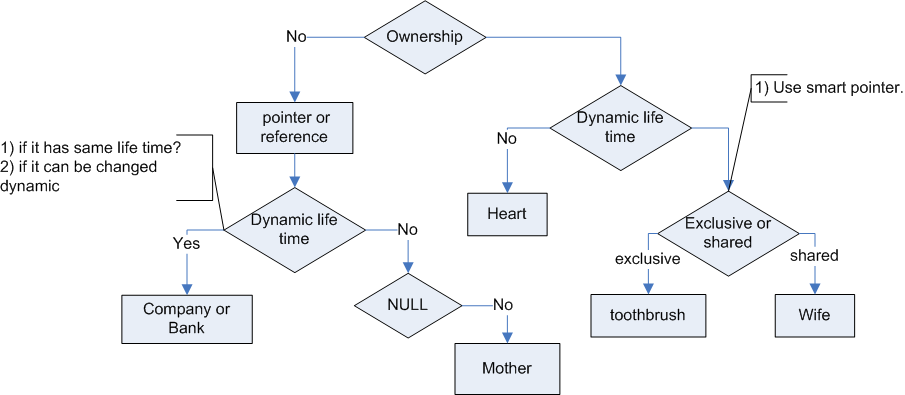
\includegraphics[width=0.92\linewidth]{pics/owner.png}
\end{center}


\begin{description}
	\item[Company or Bank] No ownership. Company is a member, It's important for you to have a work and it used by many member functions. so it's a member. For Bank,you just use it when you want to get Money, so use it in the function as parameter. Company is associate relationship and Bank is dependency relationship.
	
	\item[Monther] No ownership. It can not be null, and can not be changed.  so we use reference. 
	
	\item[Heart] Ownership, same life time, (No dynamic life)
	
	\item [Toothbrush] Ownership, dynamic life, and exclusive ownership, so we use unique\_ptr
	
	\item [Wife] Ownership, dynamic life, and shared ownership, so we use shared\_ptr
\end{description}


\end{itemize}

\subsection{Examples}
\begin{itemize}
	\item OOP example 1: If it's a car-engine (Composition) relationship, and it's compiler-given(not dynamic), just use \textbf{member obj.}   Pay attention, If engine has no default constructor, you have to use initialization list in car ctor.  initialization list can be used to call base ctor.
\begin{lstlisting}[frame=single, language=c++]
class Car{
	Engine eng; // member obj, not use pointer here.
	Car(int carArg, int engArg): eng(engArg){}
}
	\end{lstlisting}
	
	
	\item OOP example 2:  If it's an peole-brush (Association) relationship, If has same life time and exclusive ownership, use \texttt{uniqu\_ptr}. If you want to change, use \texttt{uniqu\_ptr} reset function or move semantic from another \texttt{uniqu\_ptr}.
\begin{lstlisting}[frame=single, language=c++]
class Person{
	unique_ptr<Brush> unpbrush;
	
	buyNewBrush(string &name){
		unpbrush.reset(new Brush());
	}
};
\end{lstlisting}
\begin{description}
	\item[Line 5:] you can't use \texttt{unpbrush= new Brush()}, unpbrush assignment only support( unique\_ptr< T > \&\&); use reset, it will make original deleted automatically. don't need destructor any more.
\end{description}
	
	\item OOP example 3: If it's wife-husband(Association) relationship, If you want to express \textbf{Strong Not Nullity}, use reference, such as Mother-Son association, You need to use initialization list to initialize mother. If Nullity, such as wife, just use raw pointer, weak\_ptr or shared\_ptr. \textbf{Because no ownership involved, don't use uniqu\_ptr at all. }
	
	\item OOP example 3-1: What's different with raw pointer, weak\_ptr or shared\_ptr?
	\begin{lstlisting}[]
class Man{
	Woman*  wife; //Can be set to nullptr. maybe change or live longer than you.
	Woman& mother;  //Must initilize mother in initial list
}
\end{lstlisting}

	
	\item OOP example 4: If it's dependency,  such as friend relationship,  Most of time, we just use pointer or reference as function parameter.
\begin{lstlisting}[numbers=none]
class Man{
	lendMoney(const Friend* mike);
    lendMoney(const unique_ptr<Friend>& mike);
    lendMoney(const shared_ptr<Friend>& mike);
}
\end{lstlisting}
\begin{description}
	\item[Line 2-4:] Just use it in function, not a member of class. Use const if don't want to change it.
\end{description}
	
	\item OOP example 5: Suppose Man and Computer(Associate from structure semantic) is has-a relationship and same life time. Don't use pointer or reference, just copy from a common computer, and maybe later you can customize your computer, and it will not effect common one.  We can copy from \texttt{commonComputer} and initialize all Worker object.  And this time use initialization list can improve efficiency.
\begin{lstlisting}[numbers=none]
class Worker{
	Computer m_desktop;
	Worker (Computer u): m_desktop(u){}
}
	
Computer commonComputer;
Worker Yan(commonComputer);
Worker Han(commonComputer);
\end{lstlisting}
	
	
	\item OOP example 6:  Change a semantic,  school may have a Bus, but \textbf{owner policy} tell us that bus can be shared by different schools. and \textbf{life time policy} tell us that bus and school has separate life time. so here, we should use \texttt{shared\_ptr}.
\begin{lstlisting}[numbers=none]
class Unit{
	shared_ptr<Bus> shr_p_bus;
}
\end{lstlisting}
	
	\item OOP example 7: One class provides a container to hold multiple objects of another type. A value container is a composition that stores copies of the objects it is holding. A reference container is an aggregation that stores pointers or references to objects that live outside the container.
	
\end{itemize}


\section{design pattern}


\subsection{Three big principles}
\begin{itemize}
	\item There are three basic rules.
\begin{enumerate}
	\item Liskov Substitution Principle----Clients (Functions and Class) that use pointers or references to base classes must be able to use objects of derived classes without knowing it.  So all overrides of virtual member functions must \textbf{require less and provide more}. So you can make substitution successfully.
	
	\item Dependence Inversion Principle. client doesn't depend on implementation. \textbf{Both clients and implementation depend on interface.}
	\begin{figure}[h]
		\centering
		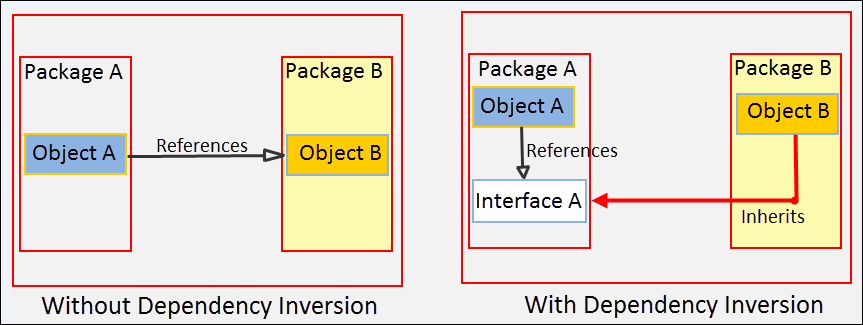
\includegraphics[width=0.7\linewidth]{pics/DIP.png}
		\label{fig:dip}
	\end{figure}
	
	\item Interface segregation principle. \textbf{Make Inferface simple and small.}
\end{enumerate}

\item Example code below.  1)LSP: \texttt{Car} can use  \texttt{GasPower} or \texttt{ElePower} without know it. 2)DIP: \texttt{Car} only is depends on \texttt{Power*} interface 3)ISP: Interface should be small and separately. An example can be seen in MI section below.

\begin{lstlisting}
class Car{
	....................
	Power* pow //Pointer or reference to the base class (Power* pow)
};

Car::start(){
	...........
	pow->ignite(); //Virtual function support dynamic-binding
}

class Power{
	virtual ignite();
};

class GasPower : public Power
class ElePower : public Power

Car car(gas);
car.start();
\end{lstlisting}

\end{itemize}


\subsection{non-leaf classes abstract and NVI}

\begin{itemize}

\item Inheritance three usage: 1) I want to inherit a interface. (pure virtual, you have to rewrite ) 2) I want to inherit a implement,but I want to change it. (virtual, you may or may not rewrite) 3) I want to inherit a implementation, but I don't want to change it. (Non-virtual, you can't rewrite it at all)
\begin{lstlisting}[numbers=none]
class shape{
	public:
	virtual draw() = 0 // you have to re-implement.
	virtual error(); // there is default implement, but you may change it.
	int objectID(); // you don't need to rewrite it.
}	
\end{lstlisting}

	\item A problem with inheriting from a concrete type is that it creates some ambiguity as to whether code which specifies a certain type really wants an object of the specific concrete type, or wants an object of a type which behaves in the fashion that the concrete type behaves. This distinction is vital in C++, since there are many cases where operations which will work correctly on objects of a certain type will fail badly on objects of derived types. The problem can be illustrated by the assignment of pointer to base class. The problem has been introduced in "More effective C++ item 33"
	

	\item "non-leaf classes abstract" rule can be found in More effective 33 "making non-leaf classes abstract" and C++ coding standards 36 "Prefer providing abstract interfaces." They all said that you should only inherit from an abstract interfaces. It also follow DIP.

	\item \textbf{When you found abstract conception appear in more than one context, you need build abstract interface for it. }


	\item NVI is making virtual functions nonpublic, and public function nonvirtual. This is similar with Template Method design pattern.  

\begin{enumerate}
	\item Prefer to make interfaces nonvirtual, using Template Method.
	
	\item Prefer to make virtual functions private.
	
	\item Only if derived classes need to invoke the base implementation of a virtual function, make the virtual function protected. For the special case of the destructor only:
	
	\item A base class destructor should be either public and virtual, or protected and nonvirtual.
\end{enumerate}

    \item About NVI, more detail can be found in "C++ coding standards Item 39" and "Virtuality herb sutter"

    \item A good example can be found below. \textbf{That is very good example, it illustrates "Non leaf abstract", "DIP", "NVI" and template method. You should learn this example and do you best to understand all ideas behinds it. }

	\centering
	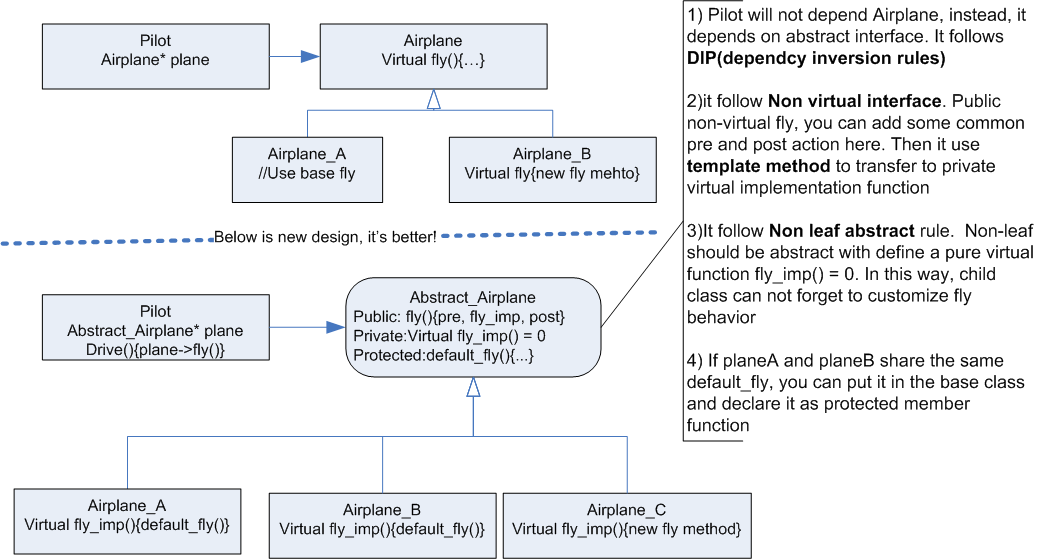
\includegraphics[width=0.93\linewidth]{pics/NVI.png}


\end{itemize}

\subsection{template method, strategy and factory template}
\begin{itemize}
	\item Comparison between these three patterns. The common points is push the change down into the child class. In factory method, we push the generating algorithm down to the child class. In strategy, we push the whole algorithm. In template method, we push the part of algorithm down to the child class.

\begin{center}
	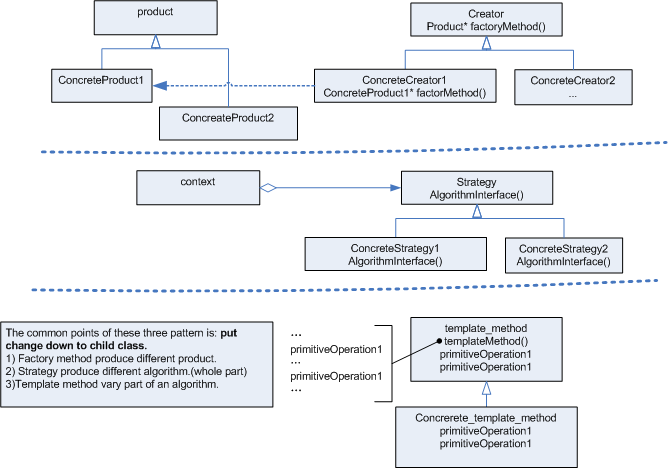
\includegraphics[width=0.93\linewidth]{pics/template_method.png}
\end{center}
	 
\end{itemize}

\subsection{MI or bridge}
\begin{itemize}
    
	\item If two superclasses of a class have a common base class,Multiple Inheritance will trigger diamond problem. It cause one grandson has two copy of grandfathers. A solution is use virtual key word: When you use this method, you need to follow New Constructor Rules, Detail can be seen in C++ primer P815.  Just look back when you really need MI.

\begin{lstlisting}[numbers=none]
Father 1: virtual public grandfather
Father2: virtual public grandfather
son : public Father1, public Father 2
\end{lstlisting}
	
	\item Suppose you have land vehicles, water vehicles, air vehicles, and space vehicles. (Forget the whole concept of amphibious vehicles for this example; pretend they don't exist for this illustration.) Suppose we also have different power sources: gas powered, wind powered, nuclear powered, pedal powered, etc. We could use multiple inheritance to tie everything together, but before we do, we should ask a few tough questions:
	
	\begin{enumerate}
		\item Will the users of LandVehicle need to have a Vehicle\& that refers to a LandVehicle object? In particular, will the users call methods on a Vehicle-reference and expect the actual implementation of those methods to be specific to LandVehicles?
		
		\item Ditto for GasPoweredVehicles: will the users want a Vehicle reference that refers to a GasPoweredVehicle object, and in particular will they want to call methods on that Vehicle reference and expect the implementations to get overridden by GasPoweredVehicle?
	\end{enumerate}
	If both answers are "yes," multiple inheritance is probably the best way to go.
	
	\item There are at least three choices for the overall design: the bridge pattern, nested generalization, and multiple inheritance. Each has its pros/cons:
\begin{center}
	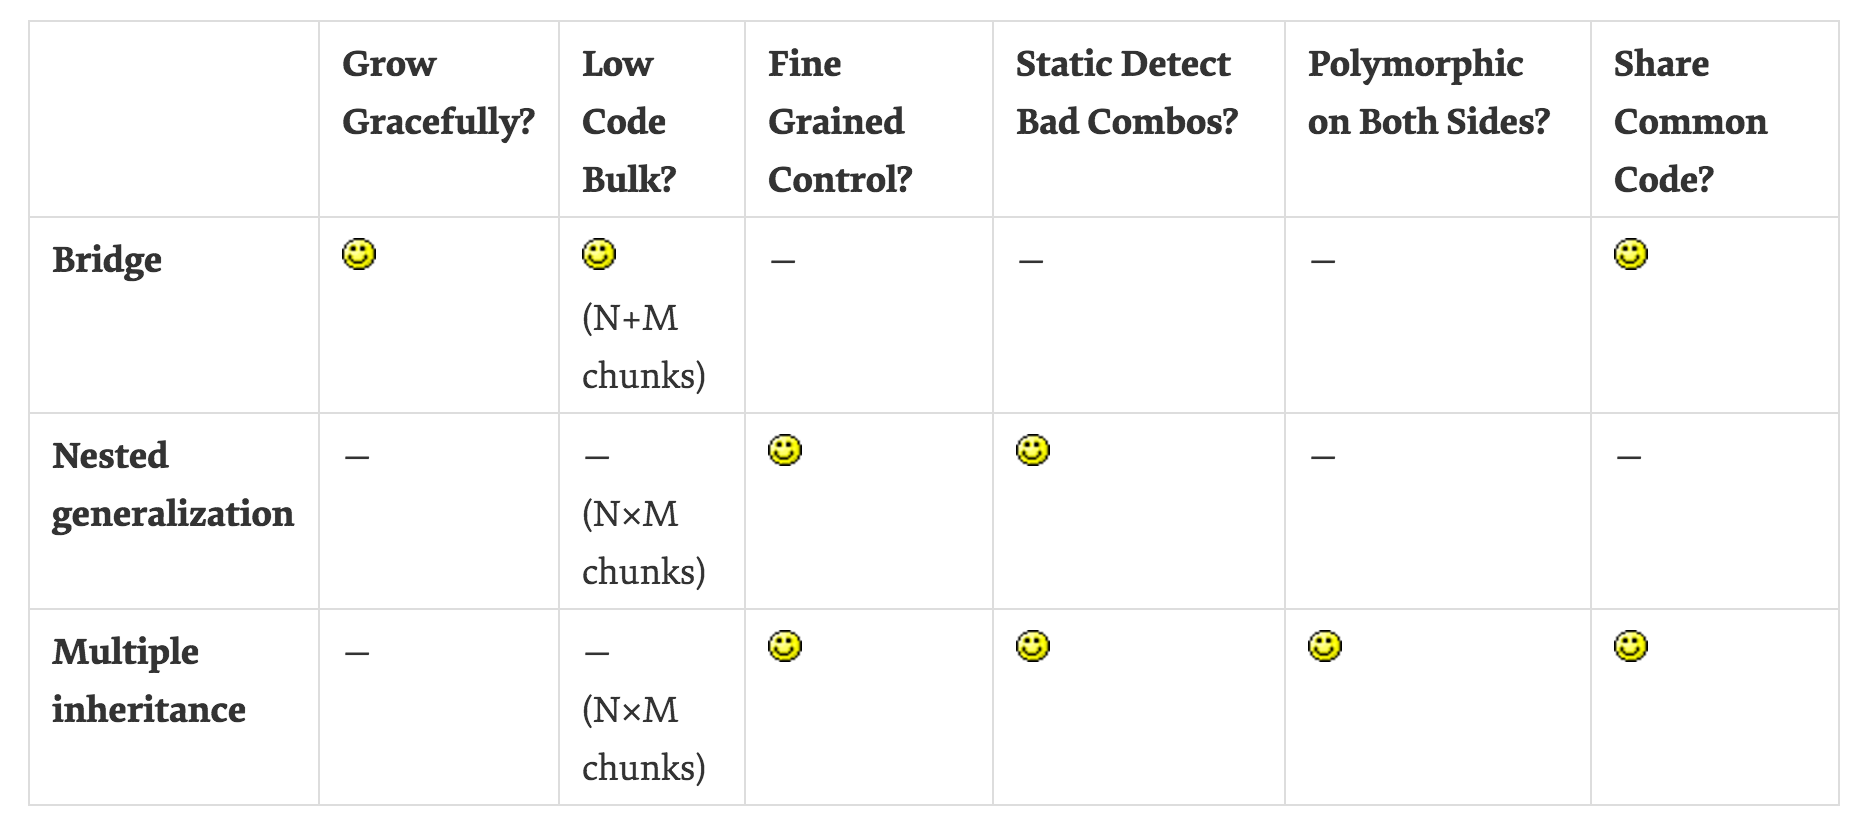
\includegraphics[scale=0.4]{pics/MI.png}
\end{center}
	
	
	\item Try especially hard to use ABCs when you use MI. In particular, most classes above the join class (and often the join class itself) should be ABCs. In this context, "ABC" doesn't simply mean "a class with at least one pure virtual function;" it actually means a pure ABC, meaning a class with as little data as possible (often none), and with most (often all) its methods being pure virtual.
	
    \item A design discussion can be seen in "C++ FAQ Inheritance-- Multiple and Virtual Inheritance"
	
\end{itemize}

\subsubsection{Comparsion between factory, bridge and visitor}

\begin{itemize}
	\item These three design pattern share the same UML structure, so I introduce them together. \textbf{Design patter is based on semantic and concrete application, not based on UML relationship and structure.}
	
	\item This is an example with bicycle and car.  We use abstract factory, bridge and visit three pattern. visit pattern also support double dispatch, how to understand it? From semantic point of view, vehicle type and refillor type (two types) decide Refill method . From source code point of view, \texttt{Vehicle} first decide a \texttt{Refillor} (\texttt{Electric} or \texttt{Oil}), once it decide one(for example \texttt{Electric}), then pass \texttt{this} pointer to decide \texttt{Refill(Car*)} or \texttt{Refill(Bicyle*)} inside of ElectricRefill class. That is \textbf{double dispatch, you give me base class pointer, I give you this.} 

		\centering
		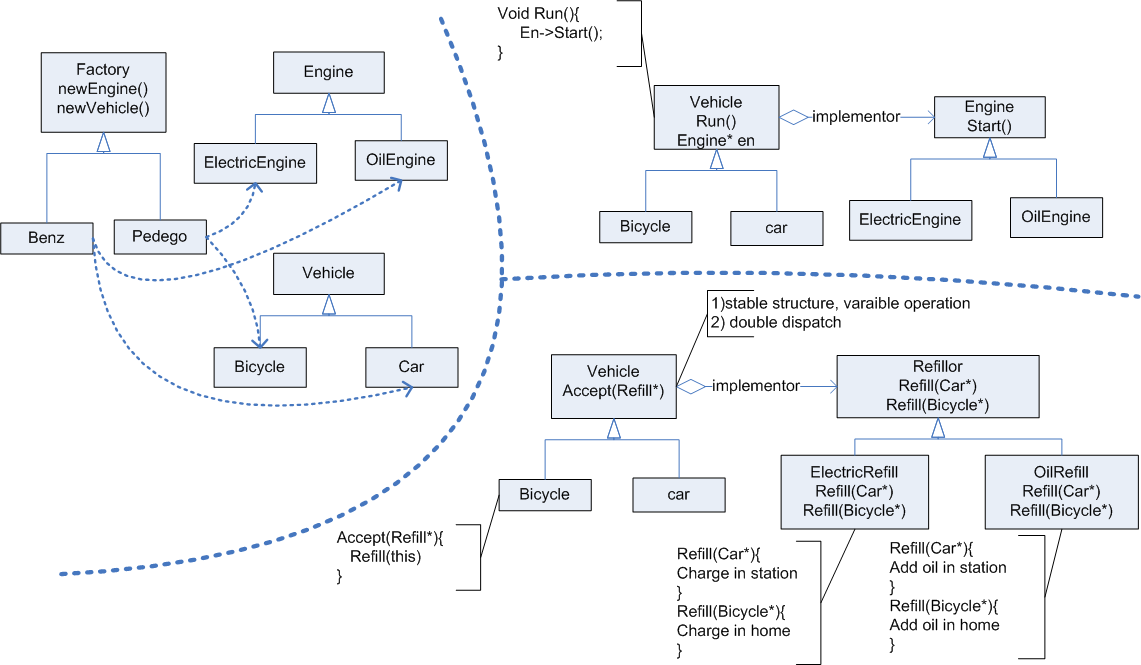
\includegraphics[width=0.93\linewidth]{pics/visitor.png}
	    
\end{itemize}

     
\chapter{Generic programming}
     
\section{Template Basic}
\begin{itemize}
    \item A simple way to simulate template is \verb=typedef int Item=; But when you change the data type, you need to modify the header file too, and you can't have \texttt{int} and \texttt{double} to template class at the same program. so C++ introduces a better method: \texttt{template<typename T>}.

    \item You should use templates if you need functions or container class(act likes) that apply the same algorithm to a variety of types. Templates are frequently used for container classes because the idea of type parameters matches well with the need to apply a common storage plan to a variety of types. A good style in template is: Use typename, not class. At the same time. simple names, such as T.
\begin{lstlisting}[numbers=none]
template<typename T> //good style
//template<class COMPLEX_T> //bad style
swap(T& a, T&b){
	.........
}
\end{lstlisting}
    \item You can have several kinds of template parameters.
\begin{enumerate}
    \item  Type Parameters: 1)Types, 2) Templates (only classes and alias templates, no functions or variable templates. Because neither function nor variable templates are type.)
	

	\item Non-type Parameters: 1)Pointers, 2)References, 3)Integral constant expressions. (That is why \texttt{constexpr} is so important.)

\end{enumerate}

\end{itemize}

\section{Type deduction}
\subsection{template type deduction}
\begin{itemize}

	\item Given below code, we will introduce the basic type deduction rules.
\begin{lstlisting}[numbers=none]
template<typename T>
void f(ParamType param);

f(expr); // deduce T and ParamType from expr
\end{lstlisting}

\begin{enumerate}
	
	\item ParamType is a Reference or Pointer, but not a Universal Reference. If expr's type is a reference, \textbf{ignore the reference part}, then pattern-match expr's type against ParamType to determine T.
\begin{lstlisting}[frame=single, language=c++]
template<typename T>
void f(T& param); // param is a reference
	
int x = 27; // x is an int
const int cx = x; //cx is a const int
const int& rx = x; //rx is a reference to x as a const int
	
f(x);    //T is int param's type is int&
f(cx);   //T is const int, param's type is const int&
f(rx);   //T is const int, param's type is const int&
\end{lstlisting}
	
	\item ParamType is a Universal Reference
	
	\begin{enumerate}
		\item If expr is an lvalue, both T and ParamType are deduced to be lvalue references.
		\textbf{although ParamType is declared using the syntax for an rvalue reference, its deduced type is an lvalue reference.}
		
		\item If expr is an rvalue, the "normal" (i.e., Case 1) rules apply.
		
		\item \textbf{Only universal reference deduction distinguishs lvalue and rvalue}
	\end{enumerate}
	
\begin{lstlisting}[frame=single, language=c++]
template<typename T>
void f(T&& param); // param is now a universal reference
int x = 27; // as before
const int cx = x; // as before
const int& rx = x; // as before
	
f(x);   //x is lvalue, so T is int& param's type is also int&.
f(cx);  //cx is lvalue, so T  and param's type are const int&.
f(rx);  //rx is lvalue, so T  and param's type are const int&.
f(27);  //27 is rvalue, so T is int, param's is therefore int&&.
\end{lstlisting}

	
	\item ParamType is Neither a Pointer nor a Reference. As before, if expr's type is a reference, \textbf{ignore the reference part}. If, after ignoring expr's reference-ness, expr is const, \textbf{ignore const too}. If it's volatile, also ignore that.
\begin{lstlisting}[frame=single, language=c++]
template<typename T>
void f(T param); // param is now passed by value
	
int x = 27; // as before
const int cx = x; // as before
const int& rx = x; // as before
f(x);   //T and param are both int
f(cx); //T and param are both int
f(rx); //T and param are both int
\end{lstlisting}

	
	\item We only drop const and volatile qualifiers for by-value parameters. For parameters that are references-to-const pointer or pointers-to-const pointer, we don't skip const. 
\begin{lstlisting}
const int ci = 2;
int& ncr = ci; //compile error
const int& cr = ci; //compile ok
int v = ci; //compile OK, v is int, not const int
\end{lstlisting}
	
	\item We only skip top const. 
\begin{lstlisting}[frame=single, language=c++]
template<typename T>
void f(T param); // param is now passed by value
	
const int* const p1 = &x;
f(p1)   //Param is const int*, top const has been skipped. 
	
const int*& rp = p1;
f(rp)  //Param is const int*, top const is default for reference. 
\end{lstlisting}
	\end{enumerate}
	
	\item \textbf{Conclusion:  Take four steps to decide:}
	\begin{enumerate}
		\item Array or function decay to pointer, if they are not used to reference ParamType
		\item Universal reference for lvalue, T is lvalue reference. (keep const)
		\item Reference is ignored
		\item For value-type ParamType, const and volatile are ignored.
	\end{enumerate}
	
	\item If you are not satisfied with automatic type deduction, you can manually specify the type.  
\begin{lstlisting}[frame=single, language=c++]
template<typename T>
void f(T param); 
	
int &x = a;
f(x)  //T is int
f<int&>(x) //T is int&
\end{lstlisting}

\end{itemize}
	
\subsection{auto type deduction in expression}
\begin{itemize}
	\item Just like a template type, auto follow the same deduction rule. Template type deduction happens when you call a function or build a customize type. \textbf{auto deduction happen when you initialize using assignment. Here just think the auto is T in the template deduction.}
	
\begin{lstlisting}[frame=single, language=c++]
auto x = 27; // x is neither ptr nor reference
const auto& rx = x; //  rx is a non-universal ref.
auto && ax = 27; // ax is universal(forwarding) ref
\end{lstlisting}

    \item \texttt{auto\&\&} is a kind of forwarding reference.
\begin{lstlisting}[frame=single, language=c++]
auto&& uref1 = x;  //x is int and lvalue, so uref1's type is int&
auto&& uref2 = cx; //cx is const int and lvalue, so uref2's type is const int&
auto&& uref3 = 27; //27 is int and rvalue, so uref3's type is int&&
\end{lstlisting}

	\item \textbf{When combine auto and brace initialization in assignment, it means \texttt{std::initializer\_list<T>}}
	
\begin{lstlisting}[frame=single, language=c++]
auto x = { 11, 23, 9 };  //x's type is std::initializer_list<int>

template<typename T>  
void f(T x);
f({ 11, 23, 9 });  //error! can't deduce type for T
	
void f(std::initializer_list<T> initList);//OK
\end{lstlisting}

	\item When use with auto, you need to be careful. The only situation where = is preferred over \verb={}= is when using auto keyword to get the type determined by the initializer.
\begin{lstlisting}[frame=single, language=c++]
auto x1 = { 1, 2 }; // decltype(x1) is std::initializer_list<int>
auto x2 = { 1, 2.0 }; // error: cannot deduce element type
auto x3{ 1, 2 }; // error: not a single element
auto x4 = { 3 }; // decltype(x4) is std::initializer_list<int>
auto x5{ 3 }; // decltype(x5) is int, not a std::initializer_list
\end{lstlisting}

	\item auto in a function return type or a lambda parameter implies template type deduction, not auto type deduction.
\begin{lstlisting}[frame=single, language=c++]
auto createInitList(){
	return { 1, 2, 3 }; //error! can't deduce type for { 1, 2, 3 }
}
	
std::vector<int> v;
auto resetV =
[&v](const auto& newValue) { v = newValue; }; // C++14
	
resetV({ 1, 2, 3 });  //error! can't deduce type for { 1, 2, 3 }
\end{lstlisting}

	\begin{center}
        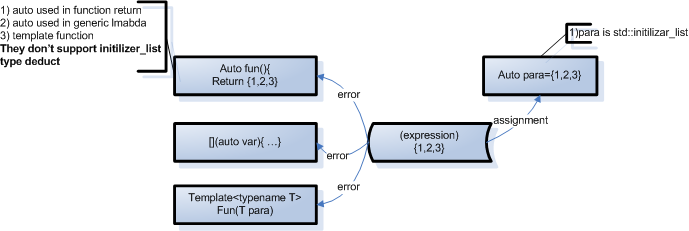
\includegraphics[scale=0.6]{pics/autotype.png}
    \end{center}

	


\end{itemize}

\subsection{auto type deduction in function}

\subsubsection{parameter type deduction}
\begin{itemize}
	\item \texttt{auto} can be used in function parameter, it is just another kind of template function.

\begin{lstlisting}[numbers=none]
void fun1(auto i){
    cout<<i<<endl;
}
		
fun1(23);  //produce two overload fun1 function.
fun1("abc");
\end{lstlisting}
    \item generic lambda( just like template lambda). auto can directly hold closures(lambda), and in C++14, It can be used as lambda parameter.
\begin{lstlisting}[frame=single, language=c++]
auto adder  = [](auto op1, auto op2){ return op1 + op2; };
\end{lstlisting}
	
	\item With help of auto, we can simplify code. 
\begin{lstlisting}[frame=single, language=c++]
auto derefUPLess =               
[](const std::unique_ptr<Widget>& p1,  const std::unique_ptr<Widget>& p2){
	return *p1 < *p2; 
};  //comparison func. for Widgets pointed to by std::unique_ptrs               

//C++14 version, values pointed to by anything pointer-like
auto derefLess = 
[](const auto& p1,  const auto& p2){
	return *p1 < *p2; 
}; 
\end{lstlisting}
	

	\item \texttt{auto \&\&}is forward reference. A good example \texttt{auto\&\&} comes(forward reference) from generic lambda. It can reserve rvalue.
\begin{lstlisting}[frame=single, language=c++]
struct Functor{
    void operator ()() const &  { std::cout << "lvalue functor\n"; }
    void operator ()() const && { std::cout << "rvalue functor\n"; }
};

int main(){
    auto perfectLambda = [](auto&& func, auto&&... params) {
        std::forward<decltype(func)>(func)(
        std::forward<decltype(params)>(params)...
        );
    };
    auto lambda = [](auto func, auto&&... params) {
        func(std::forward<decltype(params)>(params)...);
    };
    
    Functor fun;
    lambda(fun);
    lambda(Functor{});
    perfectLambda(fun);
    perfectLambda(Functor{});
}
\end{lstlisting}

\begin{lstlisting}[frame=single, language=c++]
lvalue functor
lvalue functor
lvalue functor
rvalue functor
\end{lstlisting}
	

\end{itemize}

\subsubsection{return type deduction}
\begin{itemize}
	\item C++11 permitted automatically deducing the return type of a lambda function whose body consisted of only a single return statement, so we don't need specify its return type.
\begin{lstlisting}[numbers=none]
[=]() -> some_type { return foo() * 42; } // ok
[=]  { return foo() * 42; } //ok,deduces "-> some_type"
\end{lstlisting}
	
	\item In C++14, this has been expanded in two ways. First, it now works even with more complex function bodies containing more than one return statement, as long as all return statements return the same type:
\begin{lstlisting}
// C++14
[=] {               // ok, deduces "-> some_type"
	while( something() ) {
		if( expr ) {
			return foo() * 42; // with arbitrary control flow
		}
	}
	return bar.baz(84); 
}                       
\end{lstlisting}
	
	\item In C++14, it now works with all functions, not just lambdas. Of course, this requires the function body to be visible.
\begin{lstlisting}[numbers=none]
auto fun1(){
    return 12;
}
\end{lstlisting}
	
	\item Below will produce compile error, because it has ambiguity.
\begin{lstlisting}[numbers=none]
auto f(int i){  // It will cause compile error.
    if ( i < 0 )
    	return -1;
    else
    	return 2.0
}
\end{lstlisting}

	\item For template function return type, we can use three different ways.
	
	\begin{enumerate}
		\item C++ 11, use auto + trailing type.
\begin{lstlisting}[numbers=none]
template <class T>
auto addFooAndBar(T const& t) -> decltype(t.foo() + t.bar()) {
    return t.foo() + t.bar();
}
\end{lstlisting}

\item C++ 14, directly use auto.
\begin{lstlisting}[numbers=none]
template <class T>
auto addFooAndBar(T const& t) {
    return t.foo() + t.bar();
}
\end{lstlisting}

		\item Usage of \texttt{decltype(auto)}, I will introduce this topic in decltype. More detail can be found in Effective Modern C++ item 3.
	\end{enumerate}
	
	\item \textbf{prefer to use function return type deduction wherever applicable, avoid trailing return type unless you really need them.} they make your code harder to read
	
	\item There are three ways to view deducted type:
\begin{enumerate}
	\item Use IDE.
	\item Use Compiler.
\begin{lstlisting}[frame=single, language=c++]
template<typename T> // declaration only for TD;
class TD; // TD == "Type Displayer"

TD<decltype(x)> xType; 
TD<decltype(y)> yType; 
//elicit errors containing x's and y's types
\end{lstlisting}
	
	\item Use \texttt{typeid} and \texttt{std::type\_info::name}
	
\begin{lstlisting}[frame=single, language=c++]
std::cout << typeid(x).name() << '\n'; 
\end{lstlisting}
	
\end{enumerate}

\end{itemize}



\subsection{decltype deduction}
\subsubsection{basic rule}
\begin{itemize}
	\item decltype has two different deducting rules when facing different kinds of expression.
	
	\begin{enumerate}
		\item Expression whose type is to be determined is \textbf{a plain variable} or \textbf{function parameter}, like x, or a class member access, like \texttt{p->m\_x.} In that case, decltype lives up to its name: it determines the type of the expression to be the declared type.  Pay attention to the difference between \texttt{decltype} and \texttt{auto}.
\begin{lstlisting}[frame=single, language=c++]
vector<int> v; // decltype(v) is vector<int>
struct S {
	int m_x;
};

int x;
const int cx = 42;
const int& crx = x;
const S* p = new S();

decltype(x) a;  // a is int, as auto a =x

decltype(cx) b; // b is const int
auto b = cx;  //auto ignore const, b is int

decltype(crx) c;  // c is const int&.
auto c = crx; //ignore reference and const, c is int

decltype(p->m_x) d; // d is int although p points to const S
auto d = p->m_x; //auto ignore const, d is int
\end{lstlisting}
		
		\item If expr is not case 1, then it's case 2. There are three different rules for case 2:
		\begin{enumerate}
			\item If expr is an lvalue, then \texttt{decltype(expr)} is \texttt{T\&}. 
			\item If expr is an xvalue, then \texttt{decltype(expr)} is \texttt{T\&\&}. 
			\item Otherwise, expr is a prvalue, and \texttt{decltype(expr)} is \texttt{T}.
		\end{enumerate}
	\end{enumerate}


\item For case 2, some complex expression examples:
\begin{lstlisting}[frame=single, language=c++]
const S foo();
const int& foobar();
std::vector<int> vect = {42, 43};

typedef decltype(foo()) foo_type;   //const
typedef decltype(foobar()) foobar_type; //const int&
decltype(vect[0]) first_element = vect[0]; //const int&
double d1, d2;
typedef decltype(d1 < d2 ? d1 : d2) cond_type; //double&
int x = 0;
typedef decltype(x < d2 ? x : d2) cond_type_mixed;  //double
\end{lstlisting}

	\begin{description}
		\item[Line 5:] \texttt{foo()} is declared as returning \texttt{const S}. The type of \texttt{foo()}
is \texttt{const S}. Since \texttt{foo()} is a prvalue, decltype does not add a reference. Therefore, \texttt{foo\_type} is \texttt{const S}.
		
		\item[Line 6:] The type of \texttt{foobar()} is \texttt{const int\&}, and it is an lvalue. Therefore, decltype adds a reference. By the C++11 reference collapsing rules, that makes no difference. Therefore, \texttt{foobar\_type} is \texttt{const int\&}
		
		\item[Line 7:] \texttt{std::vector<int>}'s operator[] is declared to have return type \texttt{int\&}. Therefore, the type of the expression \texttt{vect[0]} is \texttt{int\&}. Since \texttt{vect[0]} is an lvalue, decltype adds a reference. By the C++11 reference collapsing rules, that makes no difference. Therefore, \texttt{first\_element} has type \texttt{int\&}.  
		
		\item[Line 9:]  The type of the expression is double, and the expression is an lvalue. Therefore, a reference is added, and \texttt{cond\_type} is \texttt{double\&}
		
		\item[Line 11:] The type of the expression is double. The expressionis a prvalue, because in order to accomodate the promotion of x to a double, a temporary has to be created. Therefore, no reference is added, and \texttt{cond\_type\_mixed} is \texttt{double}.  For a conditional expression (?:) to be an lvalue (again, in broad and simple terms), the second and third operands must be lvalues of the same type. This is because the type and value category of a conditional expression is determined at compile time and must be appropriate whether or not the condition is true. If one of the operands must be converted to a different type to match the other then the conditional expression cannot be an lvalue as the result of this conversion would not be an lvalue.
	\end{description}

\end{itemize}

\subsubsection{decltype usage}
\begin{itemize}
	\item decltype case 2 rule mainly used in deducting template function return value.
\begin{lstlisting}[frame=single, language=c++, mathescape=true]
template<typename T, typename U>
auto eff(T t U u) -> decltype(T*U){
....
}
\end{lstlisting}

	\item When the function return a lvalue reference, auto will not work here(skip reference), only decltype can keep reference properly.
\begin{lstlisting}
template<typename Container, typename Index>  //C++11 syntax
auto authAndAccess(Container& c, Index i) -> decltype(c[i]){
	authenticateUser();
	return c[i];
}

template<typename Container, typename Index> // C++14 syntax
decltype(auto) authAndAccess(Container& c, Index i) { 
	authenticateUser();                               
	return c[i];
}
\end{lstlisting}
\begin{description}
	\item[Line 8:] \textbf{Pay attention to decltype(auto), it deducts reference type.}
\end{description}
	
	\item Below is example about using decltype on xvalue. The whole code need extra explanation here:
	\begin{enumerate}
		\item Need \texttt{Container\&\& c} to accept both lvalue and rvalue.
		\item Inside function, \texttt{c} need to be forward. that is common rule for forward reference.
		\item Forward return xvalue, then when we return this value, we also need keep it as xvalue.
		\item That is why decltype rule come from: "If expr is an xvalue, then \texttt{decltype(expr)} is \texttt{T\&\&}".
		\item Outside of function, return is xvalue, so we can move it efficiently. that is the whole story for the below code. 
	\end{enumerate}
\begin{lstlisting}[frame=single, language=c++, mathescape=true]
template<typename Container, typename Index> // final c++11
auto authAndAccess(Container&& c,Index i)
         ->decltype(std::forward<Container>(c)[i]){
	authenticateUser();
	return std::forward<Container>(c)[i];
}

template<typename Container, typename Index> // final c++14
decltype(auto) authAndAccess(Container&& c, Index i) {
	authenticateUser();
	return std::forward<Container>(c)[i];
}

auto s = authAndAccess(queue,5);
auto s = authAndAccess(std::move(queue),5); 
\end{lstlisting}
\begin{description}
	\item[Line 11:] If \texttt{Container} is xvalue, then \texttt{Container[]} is also xvalue. 
	
	\item[Line 14 and 15:] Both lvalue and rvalue work here, because \texttt{authAndAccess} uses forward reference. 
\end{description}

	
	\item The use of \texttt{decltype(auto)} is not limited to function return types. It can also be convenient for declaring variables when you want to apply the decltype type deduction rules to the initializing expression.
\begin{lstlisting}[frame=single, language=c++, mathescape=true]
Widget w;
const Widget& cw = w;

auto myWidget1 = cw;  //auto type deduction: myWidget1's type is Widget.
decltype(auto) myWidget2 = cw; myWidget2's type is  const Widget&
\end{lstlisting}
	
	\item An important property of decltype is that its operand never gets evaluated. For example, you can use an out-of-bounds element access to a vector as the operand of decltype with impunity:
	
\begin{lstlisting}[frame=single, language=c++, mathescape=true]
std::vector<int> vect;
assert(vect.empty());
typedef decltype(vect[0]) integer; 
\end{lstlisting}

\begin{description}
	\item[Line 3:] Although vect is empty now, we still can use \texttt{vect[0]} in decltype.
\end{description}
	
	\item Another property of decltype is that when decltype(expr) is the name of a plain user defined type (not a reference or pointer, not a basic or function type), then decltype(expr) is also a class name. This means that you can access nested types directly:
\begin{lstlisting}[frame=single, language=c++, mathescape=true]
template<typename R>
class SomeFunctor {
public:
	typedef R result_type;
	result_type operator()() {
		return R();
	}
SomeFunctor(){}
};

SomeFunctor<int> func;
typedef decltype(func)::result_type integer;  //You can access nested type
\end{lstlisting}
	
	\item  \textbf{If you're declaring variables inside a class.} Instead of typing out the full name of the type of the iterator, you can use decltype:, you can't use auto.  This works because decltype doesn't actually execute the expression given as its argument-- it is only used by the type checker to determine a type.
\begin{lstlisting}[frame=single, language=c++, mathescape=true]
class A {
	std::vector<std::pair<int, std::string>> array;
	decltype(array.begin()) iter; 
};
\end{lstlisting}
\begin{description}
	\item[Line 3:] You don't need initialization expression here. you can't use auto here, because auto need initialization expression
\end{description}
	
	\item We could have also done the above example with \texttt{declval}. It allows you to use decltype without constructing the object. The type doesn't even need a default constructor, and in fact, it can be used with an incomplete type. The above example could be rewritten as:
	
\begin{lstlisting}[frame=single, language=c++, mathescape=true]
template <typename C>
decltype(std::declval<const C>().begin())
foo(const C& c){
	return one iterator of c
}
\end{lstlisting}
	
	\item \texttt{declval} is commonly used in templates where acceptable template parameters may have no constructor in common, but have the same member function whose return type is needed.
	
\begin{lstlisting}[frame=single, language=c++]
struct Default {
	int foo() const { return 1; } 
};

struct NonDefault{
NonDefault(const NonDefault&) { }
int foo() const { return 1; }
};
	
decltype(Default().foo()) n1 = 1;    //type of n1 is int
//decltype(NonDefault().foo()) n2 = n1;  
decltype(std::declval<NonDefault>().foo()) n2 = n1; //It's OK now, n2 is int
\end{lstlisting}
\begin{description}
	\item[Line 11:]  error: no default constructor, In order to resolve this problem, we have to use \texttt{declval}
\end{description}
	
\item Why decltype has so complex definition about type deduction?
\begin{enumerate}
	\item the final specification of decltype represents a compromise between two different possible points of view. One point of view is that decltype should be a way to retrieve and reuse the type of a variable as declared in the source code: I declared a variable x of type T at some point in my code. Now I want to use that type for some other purpose, like making a typedef, or specify the return type of a function. I don't want to repeat myself, so give me a way to recover the declared type of my variable, exactly the way I originally wrote it. If that declared type has a reference and/or a const or volatile qualifier on it that I don't want, I'll remove that myself, thank you very much. This is what Case 1 of the specification of decltype does.
	
	\item  The second point of view that originates in the needs of library writers. They often find themselves in a situation where the return type of a function needs to be the type of some expression, typically something that depends on template parameters. They want to be able to write below source code:
\begin{lstlisting}
auto foo([...]) -> decltype(expr) {
template <typename T>
auto array_access(T& array, size_t pos) -> decltype(array[pos]) {
return array[pos];
}

std::vector<int> vect = {42, 43, 44};
int* p = &vect[0];

array_access(p, 2) = 46;
}
\end{lstlisting}
\begin{description}
	\item[Line 10:] Where the pointer p is used to access the element, could not be made to work without having decltype add a reference: the type of p[2] is int, any way you turn it. There is no reference in sight here. But p[2] is an lvalue, and by letting decltype add references to lvalues, we can get the desired effect. 
	
	\item[Source code:] \textbf{Most of expression is rvalue, but array[pos] is lvalue.} This is the key to understand decltype deduct rule for expression.
\end{description}

\item However, the reference that decltype adds is not always what you want. It happens frequently that you need to remove it with \texttt{remove\_reference}. 
\begin{lstlisting}
template<typename T, typename S>
auto fpmin(T x, S y) -> decltype(x < y ? x : y) {
	return x < y ? x : y;
}  //Error implementation 

template<typename T, typename S>
auto fpmin(T x, S y) ->
typename std::remove_reference<decltype(x<y?x:y)>::type
{
	return x < y ? x : y;
} //Correct implementation.
\end{lstlisting}
\begin{description}
	\item[Line 1 to 4:] If x and y are the same type, it will return reference. Return reference of local object is always HORRIBLE!.
\end{description}

	\item In summary: decltype rule 1 is for declaring variable, decltype rule 2 is for \textbf{deducting type for return value from function.} That is very important to know this for you to understand decltype rule 2.  When the return expression is \texttt{a[]}, because it's lvalue, so we need to return lvalue reference. When the return expression is \texttt{std::move()}, because it's xvalue, so we need to return \texttt{T\&\&}. The left 99\% are all expression, such as 1+2, they return prvalue, so we just return the type for the prvalue, for 1+2, we return \texttt{int}, that is all!
	
\end{enumerate} 
\begin{center}
	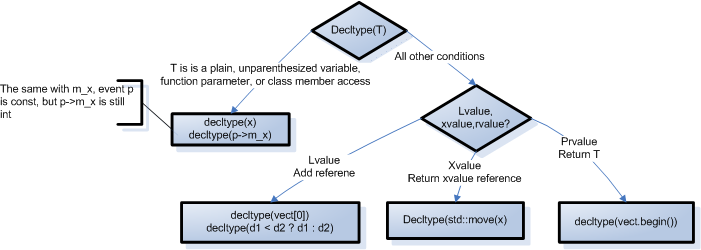
\includegraphics[scale=0.65]{pics/decltype.png}
\end{center}


\item Basic knowledge of decltype detail can be found "How decltype Deduces the Type of an Expression: Case 1"

\end{itemize}

\subsection{summary}
\begin{itemize}
	\item \texttt{auto}, template T and decltype are three kinds of type deduction contexts. \texttt{auto} and template T are almost same, beside when we meet \texttt{initilizaer\_list}.  

	\begin{center}
		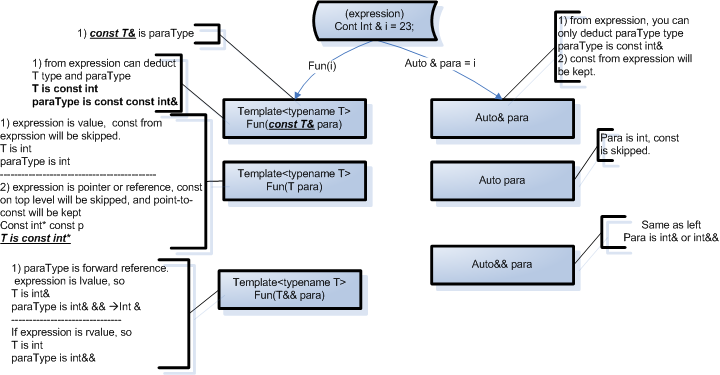
\includegraphics[scale=0.6]{pics/type_deduct.png}
	\end{center}
	
	\item decltype are quite different with the other \texttt{auto} and template T. When you use decltype(auto), \textbf{auto tell compiler to automatically type deduction, but please use decltype rules.} They are most used when we deal with some expression which return back lvalue, such as \texttt{a[0]}, in this way, if you use auto, it will ignore reference. but decltype will keep it. 
	
	\item decltype can be used in a wider variety of contexts, such as typedefs, function return types, and even in places where a class name is expected. There are two different ways in which decltype(expr) can work, depending on the value of category of expression.
	

\end{itemize}

\section{template specialization}
\subsection{class template specialization}
\begin{itemize}
	\item Class templates can be partially specialized, and the resulting class is still a template. Partial specialization allows template code to be partially customized for specific types in situations, such as:

	\begin{enumerate}
		\item A template has multiple types and only some of them need to be specialized. The result is a template parameterized on the remaining types.

		\item A template has only one type, but a specialization is needed for pointer, reference, pointer to member, or function pointer types. The specialization itself is still a template on the type pointed to or referenced.
		
		\item Three kind of partial specialization:
		\begin{enumerate}
			\item specialize one or more of types.
\begin{lstlisting}[frame=single, language=c++]
template<class T1, class T2>
class A{
}

template<class T1>
class A<T1, int>{  // must have <> after class name
}		
\end{lstlisting}				
			
			\item specialize to point or reference type.
\begin{lstlisting}[frame=single, language=c++]
template<class T>
class A{
}

template<class T>
class A<T*>{  // must have <> after class name
}		
\end{lstlisting}	
			\item specialize to another template.
\begin{lstlisting}[frame=single, language=c++]
template<class T>
class A{
}

template<class T>
class A<vector<T> >{  // must have <> after class name
}			
\end{lstlisting}	

		\end{enumerate}
	
		\item Another example of class template specification. You can see that there is three levels, It become narrower and narrower: 1) base template, 2)partial specialization 3) explict(full) specialization of member.
\begin{lstlisting}[frame=single, language=c++]
template <class T>
class Storage{
	T m_value;
public:
	Storage(T value){
	m_value = value;
}

template <class T>
class Storage<T*>{
	T* m_value;
public:
Storage(T* value){
	m_value = new T(*value);  //To make deep copy
}

template <>  //See an empty <> for fulll specialization.
Storage<char*>::Storage(char* value){
	// Figure out how long the string in value is
	int length = 0;
	while (value[length] != '\0')
		++length;
}
\end{lstlisting}
\begin{description}
	\item[Source code:] Line 1 is base template, line 9 is partial specialization and line 17 is Full specialization of constructor for type \texttt{char*} 
\end{description}

\end{enumerate}

    \item Keep the design of a template in mind and not use it blindly. When you input pointer as typename, you should be on high alert. If common template can't deal with pointer type very well, you can define a partial specializations. Pay attention the specialization of declaration. it should be after the basic template.

\begin{lstlisting}[frame=single, language=c++]
template <typename T>
class Foo //general one

template <typename T>
class Foo<T*> //partial specializations.
\end{lstlisting}

\end{itemize}

\subsection{Function template specification}
\subsubsection{Basic knowledge about function template specification}
\begin{itemize}

    \item For template function, there is overload and full specialization, for template class, there is full and partial specialization. \textbf{Template function doesn't support partial specialization}, because it can use overload to reach the same result. In another word, If you want to have custom implementation of function with same name, use overload function, if you need  custom implementation of class with same name, use partial specialization.

    \begin{enumerate}
	\item You can explicit(full) specialization of template class. 
	\item You also can explicit(full) specialization of template function. 
	\item You can explicit(full) specialization of member in template class. 
\begin{lstlisting}
template<> int f(int) //full specialization must have a empty template<>
template<>   //same as above
class S<void>
\end{lstlisting}
	\end{enumerate}


    \item Explicit Specialization: Because for \texttt{char *}, you can't use > , but use \texttt{strcmp}.  So you need to build explicit specialization Version. The prototype and definition of an explicit specialization should be preceded by template<> and should mention the specialized type by name.
	
\begin{lstlisting}[numbers=none]
Template<typename T>
      void sortedArrary(T) {...};

template<> void sortedArray<const char *>(){...}
\end{lstlisting}
\begin{description}
	\item[Source code:] There is empty<> after template, there is non-empty<> after funciton name. For the class, we follow the same the syntax.
\end{description}

\item Some explicit specification syntax.
\begin{lstlisting}[frame=single, language=c++]
template<typename T>
void foo(T param);

void foo(int param); //regular funciton, not a specialization. it is an overload

void foo<int>(int param); //ill-formed, not recommend, no template keyword at all

template <> void foo<int>(int param){...} //normal explicit specialization
template <> void foo(int param); {...} //save as above

template void foo(int param);  //explicit instantiation.
template void foo<int>(int param); //explicit instantiation.
template void foo<>(int param); //explicit instantiation.
\end{lstlisting}

\item There seems to be (a lot) of confusion regarding explicit instantiation and specialization. The code I posted above deals with explicit instantiation. The syntax for specialization is different. Here is syntax for specialization: Note that angle brackets after template!

\begin{lstlisting}
template <typename T> void func(T param) {} // definition

template void func<int>(int param);  //explicit instantiation.

template <> void func<int>(int param) {}  //explicit specialization
\end{lstlisting}
\begin{description}
	\item[Source code:]\textbf{For specialization,there is empty <> after template keyword, for instantiation, there is not empty <> after template keyword.}
\end{description}

\end{itemize}

\subsubsection{overload or full specification of function template}

\begin{itemize}
	\item  If you want to customize a function base template and want that customization to participate in overload resolution (or, to always be used in the case of exact match), make it a plain old function, not a specialization. And, if you do provide overloads, avoid also providing specializations. Detail you can google" Why Not Specialize Function Templates?" \textbf{prefer to use overload than template function specification.}

	\item For function template, we pick up which function will be used in this order: 
	\begin{enumerate}
		\item From overload function template pick one,
		\item specialization version of function template which is picked in the first step.
	\end{enumerate}

\begin{lstlisting}[frame=single, language=c++]
template<typename T>
f(T t);  //#1

template< >f<int*>(int* t) #2

template<typename T>
f(T* t); //#3

template<> f<int> f( int* t) //#4

int * p;
f(p) // #4>#3>#2>#1
\end{lstlisting}
\begin{description}
	\item[Source code:] The First step, we picked f(T* t) function template \#3, then select a specialization of this funciton template \#4. The \#1 and \#2 are not considered at all.
\end{description}

\item For above example, If you omit type inside <> after function name f, It will depends on location.
\begin{lstlisting}[frame=single, language=c++]
template<typename T>
f(T t);  //#1

template< >f<>(int* t) //#2 is specialization of #1

template<typename T>
f(T* t); //#3

template< >f<>(int* t) //#4 here is specialization of #3

int *p; 
f( p ); 
\end{lstlisting}
\begin{description}
	
	\item[Line 12:] If put specialization at line 4, it will call \#3. Although we have a very match specification, it's not be picked up and it's not what we want.  Why this happen? because specification didn't join the overload processing. The first, we only see two overload template functions: \texttt{f(T t)} and \texttt{f(T* t)}. In this way, \texttt{f(T* t)} is picked up. If we put specification in line 4, then it is specification of \#1, that is why it's omitted. If put specialization at line 9, it will call \#4.
	
	\item[Source code:] You need to know two points to understand above code: 1)specification doesn't join the overload processing. 2) Which base to pick up depends on specification location.
\end{description}

	\item Why we need a overload template function? Because not all type support the same operation. For example, in your template function, you use = operator as assignment, but when you use array for this template function type, array doesn't support assignment with operator =.
\begin{lstlisting}[numbers=none]
template <typename T>
void swap(T a[], T b[], int n)

template <typename T>
void swap(T &a, T &b )
\end{lstlisting}

	\item Overload is different with Specializations, Overload means that you have different function signatures. Specialization have the same function signature.

	\item Explicit specializations usually need define all the implementation in it. If there is a lot of repetition. There are two helpful options: 
\begin{enumerate}
	\item Add a special function which is just suitable for certain type. 
\begin{lstlisting}[numbers=none]
template <typename T>
class A{
public:
void onlyForInts(T t){
	static_assert(std::is_same<T, int>::value, "Only ints!");
}

protected:
	std::vector<T> myVector;
};

A<int> i;
i.onlyForInts(1); // works !

A<float> f;
//f.onlyForInts(3.14f); // does not compile !
\end{lstlisting}

\item Use type trait and overload, select at the compile time. See enable\_if example below.

\end{enumerate}

    \item pointer sometimes need to be deal with differently, at that time we need partial specialization of template class. A very good article is:\\ https://www.learncpp.com/cpp-tutorial/13-8-partial-template-specialization-for-pointers/. 

    \item A very good article about specialization is chapter 12 in "C++ template: The complete guide". Remember, you should read each sentence in this chapter.
    
    \item Some good articles:\newline
    "Why Not Specialize Function Templates?" .
    \newline
    "Why Argument Dependent Lookup doesn't work with function template dynamic\_pointer\_cast". 
    \newline
    "C++ template function taking template class as parameter".
\end{itemize}


\section{Template instantiation}

\subsection{Difference between instantiation and specification}
\begin{itemize}
    \item There are two confusing words in template domain, let's make them clear. What is \textbf{instantiation and specification?}
\begin{enumerate}
	\item C++ uses implicit or explicit instantiation to generate a specialized class or function definition from template. For implicit, you have to declare an variable, but for explicit, you don't need to declare an obj; \textbf{declare an variable or use template keyword}. These two instantiations are all based on existing template implementation.
	
\begin{lstlisting}[frame=single, language=c++]
template<typename T, int n>
class ArrayTP...
	
ArrayTP<int, 100> stuff //define a variable, implicit
	
template ArrayTP<string, 100>; //use template keyword and< >, explicit
\end{lstlisting}

	\item Explicit specialization is defining a different template implementation for certain type. For example, For bool type, we can use optimize array storage method.
\begin{lstlisting}[frame=single, language=c++]
template<typename T, int n>
class ArrayTP{...common implementation}
	
template<>
ArrayTP<bool, 100>{...specific implementation}
\end{lstlisting}
\begin{description}
	\item[Line 4 and 5:] There is empty<> after template. At the same time, you should give your own implementation.
\end{description}
	
	\item Implicit, explicit instantiation and explicit specialization are all \textbf{specialization}. Because it produces a real function definition that uses specific types, The last result is not template at all 
	
	\item Partial specialization is different with explicit(full)specialization. Partial specialization makes generic template a little narrow, but the result is still template. 
	 
	\item For class template, specialization includes explicit(full) specialization and partial specialization.
\begin{lstlisting}[frame=single, language=c++]
template<> class Pair<int,int>{...}; // full specialization 
template<typename T1> class Pair<T1, int>{...}; //partial specialization 
\end{lstlisting}
	
	\item Non type argument and default type argument only define one template body(only one recipe). But specialization need to define a generic template body(one recipe), For another type, It need to define a different template body(another recipe), because the code will be different with generic one.
	 
	 \textbf{Instantiation is different with specialization.  For instantiation, it will use template function to produce function body, but for specialization, you have to redefine you own function body }
	 
\begin{lstlisting}[frame=single, language=c++]
Template<typename T>
void sortedArrary (T t) {...};

template void sortedArray<Person>(Person);

template<> void sortedArray<Person>(Person t){  //it is full specialization.
.... //give you own definition of template fun body.
};
.
\end{lstlisting}

	\item For function template, there is no partial specialization, So explicit specialization is complete specialization.
\end{enumerate}


	\item Instantiation happen in compiling time, not running time. When you declare a variable, It will instantiation. (It will make compiling time longer). So all the template definition must be put in head file. 
	
\end{itemize}

\subsection{overload resolution rule}
\subsubsection{Name look up}
\begin{itemize}
    \item A name is a qualified name if the scope to which it belongs is explicitly denoted using a scope-resolution operator (::) or a member access operator (. or ->). For example, \texttt{this->count} is a qualified name.

    \item  A name is a dependent name if it depends in some way on a template parameter.  For example, \texttt{std::vector<T>::iterator} is usually a dependent name if \texttt{T} is a template parameter, but it is a nondependent name if \texttt{T} is a known type alias (such as the \texttt{T} from \texttt{using T = int}).

	\item Qualified names are looked up in the scope implied by the qualifying construct. If that scope is a class, then base classes may also be searched. However, enclosing scopes are not considered when looking up qualified names. 

	\item In contrast, unqualified names are typically looked up in successively more enclosing scopes (al-though in member function definitions, the scope of the class and its base classes is searched before any other enclosing scopes). This is called ordinary lookup. A more recent twist to the lookup of unqualified names is that—in addition to ordinary lookup—they may sometimes undergo argument-dependent lookup (ADL).
            
    \item \textbf{compiler will parse the template definition before it instantiation.} Why? It's a compiler, not a macro processor. Errors in the template itself won't be detected as long as it is only instantiated with 'friendly' types that don't trigger the errors: for example, if the template assumes that the type always has such-and-such a method.

    \item C++ Coding standards 65 states customization of point. In order to understand it. You need to understand two basic conceptions: \textbf{"two phases lookup"} and \textbf{"dependent name"}.  Two phases lookup can see "Dependent name lookup for C++ templates" and "Two-Phase or Not Two-Phase: The Story of Dependent Names in Templates". Just google them.
\end{itemize}


\subsubsection{resolution rule}
\begin{itemize}
	\item Given a function name, you can have regular, template and explicit specialization template. When pick a function, regular> specialization> template. function picking ranking from best to worst is:
	\begin{enumerate}
		\item Exact math, regular function.
		\item Template if you have define the same template function name.
		\item Conversion by promotion.
		\item Conversion by standard conversion.
		\item user-defined conversion.
	\end{enumerate}

\item What is exact match. There are table below:

\begin{center}
	\begin{tabular}{|c|c|}
	\tophline
	Actual argument & Formal argument \\
	\tophline
	type-name & type-name \& \\
	\tophline
	type-name \& & type-name \\ \tophline
	type-name [ ] &  type-name* \\ \tophline
	type-name ( argument-list ) & ( *type-name ) ( argument-list ) \\ \tophline
	type-name  & const type-name \\ \tophline
	type-name  &  volatile  type-name \\ \tophline
	type-name*  & const type-name*  \\ \tophline
	type-name*  & volatile  type-name*  \bottomhline
	\end{tabular}
\end{center}

	\item About exact match, there are three results:
	\begin{enumerate}
		\item If there are two exact matches, compiler can't distinguish them, then it will report error.
		
		\item If reference and pointer, even there are two exact match, It will pick up first according to const.
\begin{lstlisting}[frame=single, language=c++]
int i = 2;

f(const int& j); //#1
f(int& j);  //#2, #2 will be selected, because i isn't const.
\end{lstlisting}

		\item If there are exact match, it will pick up before template, even template has EXACT specification.
\end{enumerate}

	\item You can tell compiler that you prefer template function over overload one.

\begin{lstlisting}[frame=single, language=c++]
template<typename T>
void f(T t);  //#1
void f(int t) //#2

f<>(2); 
\end{lstlisting}
\begin{description}
	\item[Line 5] Tell compiler to use \#1, not \#2. Pay attention, there is <> after function name f.
\end{description}

    \item \textbf{Overload resolution steps are introduced here.} More explanation of below figure can be found below from code p1 to code p6:

\begin{figure}[ht]
	\centering 
	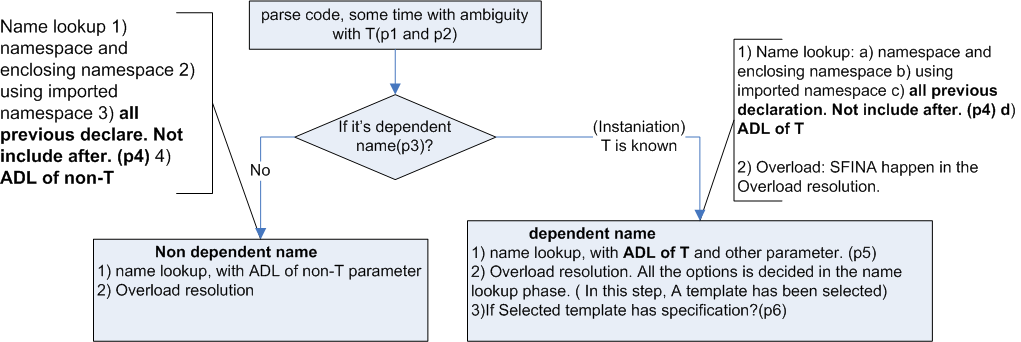
\includegraphics[width=0.8\linewidth]{pics/template.png}
	\caption{Template name look up}
	\label{fig:command}
\end{figure}

\begin{enumerate}

\item Below are p1 and p2 source code: \textbf{In these two examples, because both are dependent name, so we have to add extra typename and template keyword to help parser to resolve the ambiguity.}

\begin{lstlisting}[frame=single, language=c++]
template <typename T> struct Base {
	typedef int MyType;
};

template <typename T> struct Derived : Base<T> {
	void g() {
		// MyType k = 2;  //error: 'MyType' was not declared in this scope
		// Base<T>::MyType k = 2;
		
		typename Base<T>::MyType k = 2;
	}
};
\end{lstlisting}
\begin{description}
	
	\item[Line 8:] error: need 'typename' before '\texttt{Base<T>::MyType}' because '\texttt{Base<T>}' is a dependent scope.
	
	\item[Line 10:] Work! By now, we are still parse the template code, no any real instantiation visible. So I should tell the compiler that \texttt{::MyType} is type name not varabile name or any other thing, the we can use this to declare a variable \texttt{k}.
\end{description}

\begin{lstlisting}[frame=single, language=c++]
struct Foo {
	template<typename U>
	static void foo_method(){
	}
};

template<typename T> void func(T* p) {
	// T::foo_method<T>(); // error: expected primary-expression before '>' token
	
	T::template foo_method<T>(); //work!. That is "template qualifier".
}
\end{lstlisting}

\item p3, change variable into the a dependent name. 
\begin{lstlisting}[]
template <typename T> struct Base {
   void f() {...}
};

template <typename T> struct Derived : Base<T> {
   void g() {
       //f(); error happen here. 
       this->f() will resolve problem.
   }
};
\end{lstlisting}
\begin{description}
	\item[Line 7:] \texttt{f()} is not dependent name, so we begin to look for this name now, but the base class doesn't exit it.(no instantiation yet), so report error.
	
	\item[Line 8:] Work, make it become dependent name so we delay the name lookup after instantiation.
\end{description}


\item p4, name look up has two stages. 

\begin{lstlisting}[]
namespace framework { // library 1
	template <typename T>
	void f(T) { puts("master");}
 
	template <typename T>
	void process(T v) { f(v); }
}
 
namespace boost {     // library 2
	template <typename T>
	struct optional {};
}
 
namespace framework {//both f and specialization are in frame work namespace
	template <typename T>
	void f(boost::optional<T>) { puts("optional<T>"); }
    
	inline void f(boost::optional<bool>) 
	                { puts("optional<bool>"); }
}
 
int main(){
	int i = 0;
	boost::optional<int>  oi;
	boost::optional<bool> ob;
  
	framework::process(i); //output three "master"
	framework::process(oi);
	framework::process(ob);
}
\end{lstlisting}

\begin{description}
	\item[Line 6:] From process function, it looks for \texttt{f} function. It looks for 1)Current namespace. 2)Using namespace. 3)All previous declaration.
	 At these time only f(T) is visible, Then add it into overload options set.  
	 
	 \item[Line 27:] Because in the f(v) at line 6, v is dependent name. When T is knowing \\ (\texttt{optional<int>}), It will search the name \texttt{f} in the boost namespace again.  \textbf{At this time, it will not search framework namespace again}
\end{description}


\item p5, In instantiation, with help of ADL, boost namespace is searched and two other functions are added into overload options.
\begin{enumerate}
	\item In line 6, we see the \texttt{f(v)}, then we just use \texttt{non-concrete-type} lookup. At this time only a \texttt{f} definition in line 3 is visible.
	
	\item In line 28, When you see \texttt{ob}, we can use \texttt{concrete-type} lookup, at this time, first, we extract concrete-type(\texttt{optional} type), then we look for boost namespace which optional type resides in. In this namespace, we found two other functions options(line 15 and line 18). Add them to overload options. 
	
	\item In line 29, Once we finish overload resolution, If we select template function, then we use concrete-type specialization look up, looks all the options before line 29. That is why we select specialization in line 18.
\end{enumerate}	

\begin{lstlisting}[]
namespace framework{  // library 1
  template <typename T>
  void f(T) { puts("master"); }
 
  template <typename T>
  void process(T v) { f(v); } 
}
 
namespace boost{      // library 2
  template <typename T>
  struct optional {};
}
 
namespace boost {      // some glue between 1 and 2
  template <typename T>
  void f(optional<T>) { puts("optional<T>"); }
    
  inline
  void f(optional<bool>) { puts("optional<bool>"); }
}
 
int main(){
  int i = 0;
  boost::optional<int>  oi;
  boost::optional<bool> ob;
  
  framework::process(i);
  framework::process(oi); //output "optional<T>"
  framework::process(ob); //output "optional<bool>"
}
\end{lstlisting}



\item p6, template specification happen in the end and after overload. 
\begin{lstlisting}[]
namespace framework{  // library 1
  template <typename T>
  void f(T) { puts("master"); }
 
  template <typename T>
  void process(T v) { f(v); } 
}
 
namespace boost{      // library 2
  template <typename T>
  struct optional {};
}
 
namespace framework{  // some glue between 1 and 2
  template <>
  void f<boost::optional<bool>>(boost::optional<bool>)
  { puts("optional<bool>"); }
}
 
int main() {
  int i = 0;
  boost::optional<bool> ob;
  
  framework::process(i);
  framework::process(ob);
}
\end{lstlisting}

			
		\item Pay attention, you can't put the specialization after calling points, otherwise it will report error. 
\begin{lstlisting}
template <typename T>
void f(T) { cout<<"master"<<endl; }

int main(){
int i = 2;
f(i);
}

template<> void f<int>(int i){ //error
cout<<"specilization"<<endl;
}
\end{lstlisting}
\begin{description}
	\item[Source code:] In line 6, compiler will generate \texttt{f(int)}, when it processes to line 9 and see another \texttt{f(int)}, it reports a kind of "duplicate" error
\end{description}

	\item Summary: 1) non-concrete-type lookup 2) concrete-type ADL look up 3) At this time overload finish, then concrete-type specialization look up.


\item Another interesting example helps you to understand previous all the examples. You can copy this code and run it, to try different combination and see the output.Please refer the previous figure and all the source examples form p1 to p6. 
\begin{lstlisting}[frame=single, language=c++, numbers=left,
stepnumber=1,]
template<typename T>
void f(T i){
	cout<<"template "<<i<<endl;
}

//template<> void f<short>(short s);
void g(void){
	//int s = 5; //output template
	short s = 5; 
	//uncomment above specification, call specification version.

	//"Specification after initialzation.
	f(s);
}

template<> void f<short>(short s){
	cout<<"specification" <<s <<endl;
}
void f(short s){
	cout<<"short " <<s<<endl;
}

int main(){
	g();
}
\end{lstlisting}

\begin{enumerate}
	\item put line 19 and line 16 two functions before function g, it will call regular exact match function \texttt{void f(short)}. 
	
	\item put \texttt{void f(short)} after function g, it will can full specification version
	
	\item comment line 6 (specification declaration). report error:\\
	error: specialization of 'void f(T) [with T = short int]' after instantiation.
	Because it has instantiation f(short) version from generic template, you can't specialize it any more.
	 
	\item \textbf{Although exact match and specification have higher order, but you you mush make it visible by declaring them before the caller.}
\end{enumerate}

\end{enumerate}

    \item A good article is "Overload resolution" in Andrzej's C++ blog. \textbf{It taught you 1) name lookup and 2)overload and 3)instanition three conception very well.}
\end{itemize}


\section{Common used template technologies}

\subsection{template parameter}

\begin{itemize}
        \item You can use more than one type parameter, or default type template parameters.
\begin{lstlisting}[numbers=none]
template <typename T1,  typename T2>
class Pair{ }
Pair<double, int> pair1;

template <typename T1,  typename T2=int>
class Pair{ }
Pair<double> pair2;
\end{lstlisting}

    \item You can use Non-Type Argument in a template. But it will cause code bloat problem. 
\begin{lstlisting}[numbers=none]
template <typename T, int n>
	class ArrayTP{
	T ar[n];
	......
}
\end{lstlisting}

    \item Type parameter can be another template class.  It's different with "template template parameter" which is introduced below.
\begin{lstlisting}[]
template<typename T> // T is int here
class A

template<typename T> //T is A<int> here
class B

B< A<int> > obj;

vector< vector<int> > matrix // 2D matrix
\end{lstlisting}

    \item What is template template parameter? An article is "Correct usage of C++ template template parameters". Another good one is "C++ Common Knowledge: Template Template Parameters". It gives a stack example. Below is bad way to declare stack template.
\begin{lstlisting}[frame=single, language=c++]
template <typename T, typename Cont>
class Stack {
public:
	~Stack();
	void push( const T & );
	//...
private:
	Cont s_;
};

Stack<int, List<int> > aStack1; // OK
Stack<double, List<int> > aStack2; // legal, not OK           
Stack<std::string, Deque<char *> > aStack3; // error!   
\end{lstlisting}
    \item We use template template parameter. 

\begin{lstlisting}[frame=single, language=c++]
template <typename T,  template <typename ELEM, 
		typename = std::allocator<ELEM> > 
		class Cont = std::deque>
class Stack {
//...
private:
	Cont<T> s_;
};
//...
Stack<int> aStack1; // use default: Cont is Deque
Stack<std::string,std::list> aStack2; // Cont is List
\end{lstlisting}
\begin{description}
	\item[Line 1:] \textbf{There is another template keyword inside of the out template arrow brackets.} 
	
	\item[Line 2:] Why you need \texttt{std::allocator} here? because \texttt{std::deque} is template calss with two template parameter.
	
	\item[Line 3:] \texttt{std::deque} is default template parameter.
	
	\item[Line 7:] You don't need to specify inside template parameter, because \texttt{Cont<T>} will help to deduct it.
	
\end{description}

\end{itemize}



\subsection{member function templates}

\begin{itemize}
	\item Use member function templates to accept
	"all compatible types." detail can be found in effective c++ item 45. An example can be found below, we define a template copy constructor member function, for a generalized copy ctor.
	
\begin{lstlisting}[frame=single, language=c++]
template<typename T>
class SmartPtr {
public:
	template<typename U> // member template
	SmartPtr(const SmartPtr<U>& other); 
...
}
\end{lstlisting}
	
	\item First give an interesting example about template class. Given a container c, accumulate all the elements in it.
\begin{lstlisting}
template<typename T> //function 1
typename T::value_type Sum(T& c){
	typename T::value_type result{};
	for(auto x : c){
		result +=x;
	}
	return result;
}

template<typename T> //function 2
T Sum(vector<T> & c){
	T result{};
	for(auto x :c){
		result += x;
	}
	return result;
}

vector<int> vi = {1, 3, 5, 7};
list<int> li = {1, 3, 4, 5};
cout<< Sum(vi)<<endl;
cout<< Sum(li)<<endl;
\end{lstlisting}
\begin{description}
	\item[Source code:] Function 1 is more generic than Function 2, because it also support list. Here there are two \texttt{Sum} funciton, because we can overload template function. You also need to know, The second template function sum has ZERO relationship with vector template.
\end{description}

	\item Next, based on previous example, we give another example.
\begin{lstlisting}
template<T>
Rational<T> operator*(const Rational<T>& lsh, const Rational<T>& rhs){
	....
}

template<typename T>
class Rational {
public:
	Rational(const T& numerator = 0, const T& denominator = 1)
	...
} 

Rational<int> oneHalf(1,2);
Rational<int> result = oneHalf*2; //Compile error
\end{lstlisting}
\begin{description}
	\item[Source code:] We can't instantiate template operator * by expression \texttt{oneHalf*2}. Why? If we implicit convert 2 to Rational<int>, then we can deduct correct and instantiate template operator *. But, why we implicit convert?, we have a function to match. Right now, we don't have any function, \textbf{Pay attention here, template function is still not real function}. So we never do implicit convert without any real function which need to be matched.  The whole story is just like chicken and egg. That's why oneHalf*2 fail here. 
\end{description}

	\item Continue the previous example, If we have a function declaration exist, then implicit convert will happen. So let's see the next source code:
\begin{lstlisting}
template<T>
Rational<T> operator*(const Rational<T>& lsh, const Rational<T>& rhs){
	....
}

template<typename T>
class Rational {
public:
	Rational(const T& numerator = 0, const T& denominator = 1){...}
	friend Rational<T> operator*(const Rational<T>& lsh,  const Rational<T>& rhs)
} 

Rational<int> oneHalf(1,2);
Rational<int> result = oneHalf*2; //Compile OK, Link error
\end{lstlisting}
\begin{description}
	\item[Line 10:] Here, you can omit <T> after Rational. Inside class template, class\_name is just class\_name<T>.
	
	\item[Line 15:] By now, Compile OK. Because when we define Rational<int>, it declare a friend function in line 10, so we can implicit convert 2 to Rational<int> to match this the function in line 10.
	
	\item[Source code:] \textbf{The Line 10 and the function which defined in Line 1 has no relationship.}. Most of people will think that they are declaration and definition relationship. it's totally wrong. In fact, the template function is still not a real function.  We need to instantiate this template to a real funciton by either implicit or explicit instantiation.
	
	\item[Source code:] The code still has link error, Why link error? because we still fail to instantiate template operator * in Line 1. That's to say, we don't have any real funciton of operator *. We have introduced why in the the previous example.
\end{description}

	\item Last, How to resolve this problem, You can give the definition inside the class directly and delete template operator* in the outside. 
\begin{lstlisting}[frame=single, language=c++]
template<typename T>
class Rational {
public:
...
	friend const Rational operator*(const Rational& lhs, const Rational& rhs){
		return Rational(lhs.numerator() * rhs.numerator(), 
			lhs.denominator() * rhs.denominator());  
	} 
};
\end{lstlisting}

	\item Perfect! Template syntax is always tricky and complex, but you can always go around it. So don't worry.

\end{itemize}

\subsection{template feature used in STL}
\begin{itemize}
	\item variable template
\begin{lstlisting}[]
template<class T>
constexpr T pi = T(3.1415926535897932385L);  // variable template	

template< class T >
inline constexpr bool is_integral_v = is_integral<T>::value;
\end{lstlisting}

	\item Alias template
\begin{lstlisting}[]
template< bool B, class T = void >
using enable_if_t = typename enable_if<B,T>::type;
\end{lstlisting}
	
	\item Specialization template will have default template argument automatically.
\begin{lstlisting}[numbers=none]
template<bool B, class T = void>
struct enable_if {};

template<class T>
struct enable_if<true, T> { typedef T type; }; //T default is void
\end{lstlisting}

\item An example of usage of \texttt{enable\_if}.
\begin{lstlisting}
template<typename T>
class MyClass{
public:
void f(T const&  x){}
    
template<typename T_ = T, typename = std::enable_if_t<!std::is_reference_v<T_>>>
void f(T&& x){}
};
\end{lstlisting}
\begin{description}
    \item[Line 6:] Pay more attention to three points here:
        \begin{enumerate}
            \item unname template parameter.
            \item \texttt{enable\_if\_t} is alias template.
            \item \texttt{is\_reference\_v} is variable template.
        \end{enumerate}
\end{description}

    \item \texttt{void\_t}. This metafunction is used in template metaprogramming to detect ill-formed types in SFINAE context.
\begin{lstlisting}
template< class... >
using void_t = void;

// primary template handles types that have no nested ::type member:
template< class, class = void >
struct has_type_member : std::false_type { };
 
// specialization recognizes types that do have a nested ::type member:
template< class T >
struct has_type_member<T, std::void_t<typename T::type>> : std::true_type { };

// default template:
template< class , class = void >
struct has_toString : false_type { };

// specialized as has_member< T , void > or sfinae
template< class T>
struct has_toString<T , void_t<decltype(&T::toString)> > 
                        : std::is_same<std::string, decltype(declval<T>().toString())>
{ };
\end{lstlisting}

\begin{enumerate}
	\item In order to understand previous code, you need to know "the default argument applies to the specialization". If you only give one type in \texttt{test<int>}, implicitly, it changes into \texttt{test<int, void>}. 
\begin{lstlisting}
template <class T, typename U = void>
class test {
public:
	test() {
		std::cout << "base" << std::endl;
	}
};
template <class T>
class test<T, float> { 
public:
	test() {
		std::cout << "sp" << std::endl;
	}
	
};
int main() {
	test<int> t; // actually, you call test<int, void> t, output base
	test<int, float>; //call specialization
	test<int, int>; //call base.
}
\end{lstlisting}
	\item If you specify \texttt{void} in specialization, then a type that's specified explicitly is preferred over one that's specified implicitly, so your specialization (which specified \texttt{void} explicitly) is preferred over the base template (which specified \texttt{void} implicitly).
\begin{lstlisting}
template <class T, typename U = void>
class test {
public:
	test() {
		std::cout << "base" << std::endl;
	}
};
template <class T>
class test<T, void> { 
public:
	test() {
		std::cout << "sp" << std::endl;
	}
	
};
int main() {
	test<int> t; //call specialization
}
\end{lstlisting}
	\item Why do we need void in the primary template? The default parameters are propagated in the specialization. So when we use \texttt{has\_toString<OurType>::value}, the default parameter comes into play and we are actually looking for \texttt{has\_toString<OurType, void>::value} both on the primary template and the specialization. In the meantime, the substitution and the evaluation of decltype are processed and our specialization has the signature has\_toString<OurType, std::string> if OurType has a serialize method that returns a std::string, otherwise the substitution fails. 
	
	\item The specialization has therefore the precedence in the good cases. \textbf{In another word, need both match primary and specialization, so even when match fail, we can return false\_type}

\end{enumerate}



\item a partial specialisation can indeed have more template parameters than the primary template. A typical example of this use is std::function: 
\begin{lstlisting}
template <class T>
struct function;

template <class R, class... A>
struct function<R (A...)>{  //R(A...) is specification and it's ONE template parameter.
  // std::function as we know it
};
\end{lstlisting}	

\end{itemize}

\section{type traits}

\begin{itemize}
	\item A type trait is a way for you to get information about the types which are passed in as template arguments at compile time, so you can make static dynamic. A type trait can return any information or customization about a type. A simple example is \texttt{is\_integer}, it just return bool type value information. A complex example is \texttt{char\_trait}. it can return a few functions. In this way, you also can think that \texttt{char\_trait} is a policy. 
	
\end{itemize}

\subsection{Class partial specialization implement trait}
\begin{itemize}
	
	\item \textbf{The most common way of implementation is template class specialization.} They are very useful for system defined type. Most of time, make default template return false, then make template specialization returns true. 
\begin{lstlisting}[frame=single, language=c++]
template <typename T>
struct is_swapable {
	static const bool value = false;
};

template <>
struct is_swapable<short> {
	static const bool value = true;
};

template <>
struct is_swapable<int> {
	static const bool value = true;
};
\end{lstlisting}

\item Another way is to build new trait based on existing trait.
\begin{lstlisting}[numbers=none]
template <typename T>
struct is_swapable {
	static const bool value = 
	std::is_integral< T >::value && sizeof(T)>=2;
};
\end{lstlisting}

	\item After C+11, we introduced \texttt{std::true\_type} and \texttt{std::false\_type}.
\begin{lstlisting}[frame=single, language=c++]
template<class T, T v>
struct integral_constant {
	static constexpr T value = v;
	using value_type = T;
	using type = integral_constant; // using injected-class-name
	constexpr operator value_type() const noexcept { return value; }
	constexpr value_type operator()() const noexcept { return value; } //since c++14
};
	
typedef integral_constant<bool,true> true_type;
\end{lstlisting}


\item \texttt{std::true\_type} use \texttt{integral\_constant}(type generator)to define a new type. \newline 
\texttt{is\_arithmetic} derived form \texttt{true\_type} or \texttt{false\_type}.
\begin{lstlisting}[numbers=none]
std::integral_constant<bool, true>

template< class T >
struct is_arithmetic : std::integral_constant<bool, std::is_integral<T>::value ||
							std::is_floating_point<T>::value> { };
\end{lstlisting}

	\item Rules need to be follow when you build type trait.
	
	\begin{enumerate}
		\item most common usage of trait is member constants ::value, such as \texttt{is\_integer<T>::value}
		
		\item You use a template structure, usually named with the type trait you are after. Eg) \texttt{is\_integer, is\_pointer, is\_void}. The structure contains a static const bool named value which defaults to a sensible state. You use a type trait by querying its value, like: \texttt{my\_type\_trait<T>::value}. A good article is "A simple introduction to type traits"
	\end{enumerate}

	\item Another kind of implementation is to use predefined type. An example can be found in iterator and container.

\begin{lstlisting}[frame=single, language=c++]
struct random_access_iterator_tag: public bidirectional_iterator_tag {};

template < ... > // template params elided
class \texttt{deque} {
	class iterator {
		public:
		typedef random_access_iterator_tag iterator_category;
	};		
\end{lstlisting}
\begin{description}
	\item[Line 7:] Insider deque, we define iterator class. We define \texttt{iterator\_category} inside iterator class. 
\end{description}

	\item Then we can use \texttt{iterator\_traits} to get \texttt{iterator\_category} defined inside deque.
\begin{lstlisting}[frame=single, language=c++]
template<typename IterT>
struct iterator_traits {
	typedef typename IterT::iterator_category iterator_category;
};
\end{lstlisting}

	\item Why don't we use \texttt{iterator\_category} inside of \texttt{deque} directly. With help of trait, we can build partial specification version for pointer, In this way, \texttt{iterator\_traits} also can deal with pointer. (array in C++)
\begin{lstlisting}[frame=single, language=c++]
template<typename T> // partial template specialization
struct iterator_traits<T*>{ // for built-in pointer types
	typedef random_access_iterator_tag iterator_category;
};
\end{lstlisting}

\subsection{SFINAE(Type deduct) to build trait}
\subsubsection{Before C++ 11}

	\item You also can understand it SFINAE. "Substitution Failure Is Not An Error". Compiler will try type deduct when it instantiate the template function or template class. when it can't deduct properly, compiler will search for another option instead of report error. 
	
	\item Use \texttt{sizeof} and \texttt{static\_cast}, these two can be executed at compile time. For example, we want to test if a class derived from another class.
\begin{lstlisting}[frame=single, language=c++]
template<typename D, typename B>
class IsDerivedFromHelper{
	class No { };
	class Yes { No no[3]; };
	
	static Yes Test( B* );
	static No Test( ... );
	public:
	enum {Is = sizeof(Test(static_cast<D*>(0))) == sizeof(Yes) };
};
	
template <class C, class P> 
bool IsDerivedFrom() {
	return IsDerivedFromHelper<C, P>::Is;
}
\end{lstlisting}

\subsubsection{If T has a certain name member function?}
	
	\item After C++11, you can use constexpr instead of sizeof, and \textbf{decltype and declval also get type in the compiling time.}. 
	
	
	\item We test if the type has "serialize" member function by using \texttt{decltype} and \texttt{declval}.
	
\begin{lstlisting}[frame=single, language=c++]
template <class T> 
struct hasSerialize{
	template <typename C>
	static constexpr 
	decltype(std::declval<C>().serialize(), bool())
	test(int /* unused */){
		return true;
	}

	template <typename C>
	static constexpr bool test(...){
		return false;
	}
	
	// int is used to give the precedence!
	static constexpr bool value = test<T>(int());
};	
\end{lstlisting}
	
	\begin{enumerate}
		\item template class \texttt{hasSerialize} accepts \texttt{T}, we usually use \texttt{hasSerialize<Foo>:value}.
		
		\item Two overload template test functions. One return true, default return false. \textbf{Why do we still need different template member function test?} That is because SFINAE only happens in template type deduction phrase, we build two template member function with typename C
		
		\item In the funciton which return true, use decltype and declval to simulate call some functions you want to judge. make these type used in function parameter or return. 
		
		\item Pay attention to the usage of \texttt{static constexpr bool}. Use test function to initialized \textbf{constexpr value} 
	\end{enumerate}

	\item Or we can use \texttt{true\_type} directly, it will make source code look simple.

\begin{lstlisting}[frame=single, language=c++]
// Primary template, inherit from std::false_type.
template <typename T, typename = std::string>
struct hasSerialize : std::false_type { };

// Partial template specialisation, inherit from std::true_type.
template <typename T>
struct hasSerialize<T, decltype(std::declval<T>().serialize())> : std::true_type { };
\end{lstlisting}

	\item Use \texttt{void\_t} to judge if has \texttt{reserve()} member function in type \texttt{T}.
\begin{lstlisting}[frame=single, language=c++]
template <typename T,
typename = void_t<>>
struct has_reserve : false_type {};

template <typename T>
struct has_reserve<T, void_t<decltype(declval<T&>().reserve(1U))>>: true_type {};
\end{lstlisting}
		
	\item use \texttt{is\_valid}
\begin{lstlisting}[frame=single, language=c++]
#include <boost/hana.hpp>
#include <type_traits>

namespace hana = boost::hana;

static auto has_length = hana::is_valid([](auto&& t)
-> decltype(t.Length()) { });

template <typename T>
auto foo(T const& t)
-> std::enable_if_t<decltype(has_length(t)){}, void>
// ^-- notice the return type 
// is a boolean integral constant
{ }
\end{lstlisting}

\subsubsection{ If T is function type? }

\item This is example to test if T is function.
\begin{lstlisting}[frame=single, language=c++]
template <class T>
struct IsFunction{
	// int (*p)[1]  pointer to array(int [1])
	// int *p[1], that is array of pointer .
	template <typename C> 
	static constexpr bool test(C (*)[1] ){
		return false;
	}
	
	template <typename C> 
	static constexpr bool test(...){
		return true;
	}
	//use 0 as pretend pointer.
	static constexpr bool value = test<T>(0);
};

int f();
IsFunction<decltype(f)>::value; //value is true 
\end{lstlisting}
\begin{description}
	\item[Line 6:] Why we need declare a pointer to array? it will make line 14 easier, we can just use 0 as pretend pointer.
	\item[Source code:] There is three types you can't use to declare array, 1) void, 2) reference and 3) function type.  About function type, I will introduce below. 
\end{description}

\begin{enumerate}
	\item what is function type?
\begin{lstlisting}
typedef int FT(); //FT is type

int f();  //f is variable
FT* fp= f;  //Usage of FT : fp is variable and type is function pointer

FT fv; 
void fv(){...} 
\end{lstlisting}
	\begin{description}

		\item[Line 6:] just like \texttt{int fv();} declare a function. How to define this variable make it linkable? Just like common function definition.
	\end{description}
	
	\item You can not define function type array.
\begin{lstlisting}
typedef int FT(); //FT is type
FT fa[3]; //compile error, error: declaration of 'fa' as array of functions
\end{lstlisting}

\end{enumerate}
\end{itemize}

\subsubsection{If T is member function type}
\begin{itemize}
	\item How to deal with member function pointer? Given an example code below, if you want to have member function pointer, its type should be: \texttt{int (A::*)() const \&} 
\begin{lstlisting}[frame=single, language=c++]
struct A {
	int fun() const&;
};
typedef int FunSignature() const&;
FunSignature A::*p = &A::fun;
\end{lstlisting}
\item When we want to use template class to deduct it, it can be used in \textbf{\texttt{U T::*}}.
\begin{lstlisting}[frame=single, language=c++]
struct A {
	int fun() const&;
};

template<class T, class U>
struct PM_traits<U T::*> {
	using member_type = U;
};

int main() {
	using T = PM_traits<decltype(&A::fun)>::member_type; 
	// T is int() const&
}
\end{lstlisting}

\item Based on previous knowledge, we can implement 
\begin{lstlisting}[frame=single, language=c++]
template< class T >
struct is_member_function_pointer_helper : std::false_type {};

template< class T, class U>
struct is_member_function_pointer_helper<T U::*> :std::is_function<T> {};

template< class T >
struct is_member_function_pointer : is_member_function_pointer_helper<
                        std::remove_cv_t<T>  {};

class A {
	public:
	void member() { }
};
// output 0 if A::member is a data member and not a function
cout<<std::is_member_function_pointer<decltype(&A::member)>::value
\end{lstlisting}
\end{itemize}

\subsection{is\_valid}

\begin{itemize}
	\item C++14 brings a small change to the lambdas but with a big impact! Lambdas accept auto parameters: the parameter type is deduced according the argument. Lambdas are implemented as an object having an newly created unnamed type, also called closure type. If a lambda has some auto parameters, its "Functor operator" operator() will be simply templated. Let's take a look:
	
\begin{lstlisting}[numbers=none]
auto l5 = [](auto& t) -> decltype(t.serialize()) { return t.serialize(); };
struct l5UnamedType{
	template <typename T> auto operator()(T& t) const -> decltype(t.serialize())} 
	// This signature is nice for a SFINAE, because it's template, 
		return t.serialize();
	}
};	
\end{lstlisting}
	
	\item We can use generic lambda to build \texttt{is\_valid} template
	
\begin{lstlisting}[numbers=none]
template <typename UnnamedType> struct container{
	// Let's put the test in private.
	private:
	// We use std::declval to 'recreate' an object of 'UnnamedType'.
	// We use std::declval to also 'recreate' an object of type 'Param'.
	// We can use both of these recreated objects to test the validity!
	template <typename Param> constexpr auto testValidity(int /* unused */)
	-> decltype(std::declval<UnnamedType>()(std::declval<Param>()), std::true_type()){
		// If substitution didn't fail, we can return a true_type.
		return std::true_type();
	}
	
	template <typename Param> constexpr std::false_type testValidity(...){
		// Our sink-hole returns a false_type.
		return std::false_type();
	}
	
	public:
	// A public operator() that accept the argument we wish to test onto the UnnamedType.
	// Notice that the return type is automatic!
	template <typename Param> constexpr auto operator()(const Param& p){
		// The argument is forwarded to one of the two overloads.
		// The SFINAE on the 'true_type' will come into play to dispatch.
		// Once again, we use the int for the precedence.
		return testValidity<Param>(int());
	}
};

template <typename UnnamedType> constexpr auto is_valid(const UnnamedType& t) {
	// We used auto for the return type: it will be deduced here.
	return container<UnnamedType>();
}

// Check if a type has a serialize method.
auto hasSerialize = is_valid([](auto&& x) -> decltype(x.serialize()) { });
Foo foo;
hasSerialize(foo);
\end{lstlisting}

\begin{center}
	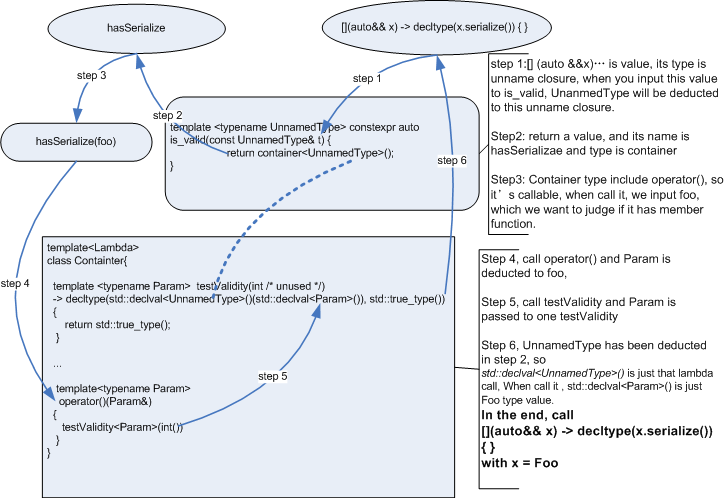
\includegraphics[scale=0.59]{pics/is_valid.png}
\end{center}

\end{itemize}



\subsection{Summary}
\begin{itemize}
	\item Common type traits implementation methods which are introduced in previous sections. 
	\begin{enumerate}
		\item template specification: \texttt{is\_integer}
		\item use basic trait: \texttt{is\_swap}
		\item use template parameter deduciton : \texttt{std::is\_function} and
		\texttt{is\_member\_function}, \texttt{is\_array}, \texttt{is\_class(T::*)}
		\item define trait in existing class : \texttt{iterator\_trait}.
		\item overload template function, deduct return or function parameter based on template parameter T's expression:  \texttt{has\_serialize}, \texttt{IsFunction}
	\end{enumerate}

	\item There are two articles which are good.
"An introduction to C++'s SFINAE concept: compile-time introspection of a class member" and "checking expression validity in-place with C++17"
\end{itemize}

\section{Usage of type trait}

\subsection{tag dispatch}
\begin{itemize}
	\item A famous usage of tag dispatch is iterator 
	\begin{enumerate}
		\item Pay attention to \texttt{iterator\_traits}. Why do we use it here? It's a template. With specialization, it can support common pointer type.
		
		\item Client side may or may not be template. For advance, it should be template, because it need template parameter Inputiterator.
		
		\item There is some tag type which need to be defined. And you should use these tags in the functions which you want to dispatched by overload resolve in compiling time. 
	\end{enumerate}
\begin{lstlisting}[numbers=none]
struct input_iterator_tag { };
struct random_access_iterator_tag { };

namespace detail {
	template <class InputIterator, class Distance>
	void advance_dispatch(InputIterator& i, 
	Distance n, input_iterator_tag) {
		while (n--) ++i;
	}
	
	template <class RandomAccessIterator, class Distance>
	void advance_dispatch(RandomAccessIterator& i,
	Distance n, random_access_iterator_tag) {
		i += n;
	}
}

template <class InputIterator, class Distance>
void advance(InputIterator& i, Distance n) {
	typename iterator_traits<InputIterator>
	::iterator_category category;
	
	detail::advance_dispatch(i, n, category);
}	
\end{lstlisting}	

    \item use \texttt{true\_type} or \texttt{flase\_type} in tag dispatch.
\begin{lstlisting}[numbers=none]
template <typename T>
int foo_impl(T value, std::true_type) {
	// Implementation for arithmetic values
}

template <typename T>
double foo_impl(T value, std::false_type) {
	// Implementation for non-arithmetic values
}

template <typename T>
auto foo(T value) {
	// Calls the correct implementation function, 
	return foo_impl(value, std::is_arithmetic<T>{});
}
\end{lstlisting}
\begin{description}
	\item[Source code] Overload function can return different types. foo's return type is \texttt{int} if it calls the \texttt{std::true\_type} overload and \texttt{double} if it calls the \texttt{std::false\_type} overload. So here we use \texttt{auto} as function return type.
\end{description}

\item Another example to use tag dispatch method.
	
\begin{lstlisting}[numbers=none]
template <typename T>
auto get_value(T t, std::true_type) {
	return *t;
}

template <typename T>
auto get_value(T t, std::false_type) {
	return t;
}

template <typename T>
auto get_value(T t) {
	return get_value(t, std::is_pointer<T>{}); 
}
\end{lstlisting}	
\end{itemize}

\subsection{enable\_if}
\begin{itemize}
	
	\item For false, \texttt{enable\_if} is empty define.
\begin{lstlisting}[numbers=none]
template <bool, typename T = void>
struct enable_if
{};

template <typename T>
struct enable_if<true, T> {
	typedef T type;
};	
\end{lstlisting}	

\item When we make the call do(25), the compiler selects the first overload: since the condition \texttt{std::is\_integral<int>} is true, the specialization of struct \texttt{enable\_if} for true is used, and its internal type is set to int. The second overload is omitted because without the true specialization (\texttt{std::is\_integral<int>} is false) the general form of struct \texttt{enable\_if} is selected, and it doesn't have a type, so the type of the argument results in a substitution failure.

\begin{lstlisting}[numbers=none]
template <typename T>
void do(typename enable_if<
std::is_integral<T>::value, T>::type &t){
	// an implementation for integral types 
}

template <typename T>
void do(typename enable_if<
std::is_class<T>::value, T>::type &t) {
	// an implementation for class types
}		
\end{lstlisting}	
	
	\item Another example which use \texttt{enalbe\_if}. \texttt{has\_serialize} trait has been introduced in the type trait section, you can see the detail there. 
	
\begin{lstlisting}[numbers=none]
template <class T>
enable_if<has_serialize<T>::value, std::string>::type
serialize(const T& obj){
	return obj.serialize();
}

// Contra-SFINAE to avoid ambiguity
template <class T>
enable_if<!has_serialize<T>::value, std::string>::type 
serialize(const T& obj){
	return to_string(obj);
}	
\end{lstlisting}	
	
	\item This technology has been used widely inside of vector.
\begin{lstlisting}[frame=single, language=c++]
template <typename T>
class vector {
	vector(size_type n, const T val);
	
	template <class InputIterator>
	vector(InputIterator first, InputIterator last);
	...
}

template <class _InputIterator>
vector(_InputIterator __first,
typename enable_if<__is_input_iterator<_InputIterator>::value &&
!__is_forward_iterator<_InputIterator>::value &&
... more conditions ...
_InputIterator>::type __last);
\end{lstlisting}	

\item In C++17, we can also use constexpr if, that make our code looks clean and simple. But the basic idea is the same. 

\begin{lstlisting}[numbers=none]
template <typename T>
auto get_value(T t){
	if constexpr (std::is_pointer_v<T>) {
		return *t;
	} else {
		return t;
	}
}
\end{lstlisting}

		\item We can also use \texttt{enable\_if} to "delete" a function for certain type. There are three points you can learn from below source code:
		\begin{enumerate}
			\item \texttt{enable\_if} can be used in template parameter deduction. Neither function paramer nor function return.
			\item pay attention \texttt{\_t} and \texttt{\_v}.
			\item Default template parameter \texttt{T\_= T} and unnamed template parameter: \texttt{typename = ...}
		\end{enumerate}
\begin{lstlisting}[numbers=none]
template<typename T>
class MyClass
{
	public:
	void f(T const&  x){}
	
	template<typename T_ = T, typename = std::enable_if_t<!std::is_reference_v<T_>>>
	void f(T&& x){}
};
\end{lstlisting}		
		
	
	\item A good article is "SFINAE and enable\_if"
\end{itemize}

\subsection{A practical example}
\begin{itemize}
    \item If we want to add some items to a kind of "container". We need to check if a container has reserve method(for example, vector). If we have this method, use it to reserve space before we use push back. Otherwise, we use push back directly.
    \item Below code build a type trait, it uses void\_t and true\_type. We have introduced before. 
\begin{lstlisting}
template <typename T, typename = void_t<>>
struct has_reserve : false_type {};
   
template <typename T>
struct has_reserve<T, void_t<decltype(declval<T&>().reserve(1U))>> : true_type {};   
\end{lstlisting}

    \item use tag dispatch to get static dynamic.
\begin{lstlisting}
template <typename C, typename T>
void _append(C& container, T* ptr, size_t size, true_type)  
{
    container.reserve(container.size() + size);
    for (size_t i = 0; i < size; ++i) {
        container.push_back(ptr[i]);
    }
}

template <typename C, typename T>
void _append(C& container, T* ptr, size_t size, false_type)
{
    for (size_t i = 0; i < size; ++i) {
        container.push_back(ptr[i]);
    }
}

template <typename C, typename T>
void append(C& container, T* ptr, size_t size) 
{ 
    _append(container, ptr, size, has_reserve<C>{}); 
}
\end{lstlisting}

    \item You can use \texttt{enable\_if} too. The syntax is little "bloat" compared with \texttt{true\_type} dispatch. But one advantage of \texttt{enable\_if} is that you can use it not only in dispatch to two different implementations, but also filter a valid type to generate valid code, for invalid type, if you don't provide \texttt{!has\_reserve<C>} match, it will generate compiling error directly.
\begin{lstlisting}
template <typename C, typename T>
enable_if_t<has_reserve<C>::value>
append(C& container, T* ptr, size_t size){
    container.reserve(container.size() + size);
    for (size_t i = 0; i < size; ++i) {
    	container.push_back(ptr[i]);
    }
}

template <typename C, typename T>
enable_if_t<!has_reserve<C>::value>
append(C& container, T* ptr, size_t size){
	for (size_t i = 0; i < size;  ++i) {
        container.push_back(ptr[i]); 
    }
}
\end{lstlisting}

	\item If you don't want to "dispatch", just want to use one function if it match.  When the input type is not valid, you hope to have compile error. Under such context, you can use decltype and declval directly.

\begin{lstlisting}[numbers=none]
template <typename C, typename T>
auto append(C& container, T* ptr, size_t size)-> 
              =decltype( declval<C&>().reserve(1U), void()){
	container.reserve( container.size() + size);
	for (size_t i = 0; i < size; ++i) {
		container.push_back(ptr[i]);
	}
}
\end{lstlisting}

\item use \texttt{if constexpr}
\begin{lstlisting}
template <typename C, typename T>
void append(C& container, T* ptr, size_t size){
    if constexpr (has_reserve<C>::value) {
        container.reserve(container.size() + size);
    }
    for (size_t i = 0; i < size; ++i) {
        container.push_back(ptr[i]);
    }
}   
\end{lstlisting}
\item In C++ 20, we can use concept directly.
\begin{lstlisting}
template<typename T>
concept HasReserve = requires(T a){
    a.reserve();
};

template <HasReserve C, typename T>
void append(C& container, T* ptr, size_t size){
    container.reserve(container.size() + size);
    for (size_t i = 0; i < size; ++i) {
        container.push_back(ptr[i]);
    }
} 
\end{lstlisting}
\begin{description}
    \item[line 6:] You can see that we use \texttt{HasReserve} here directly. The whole code is very clear, That is why we call concetp as "future of generic programming" 
\end{description}



\end{itemize}

\subsection{Summary}
\begin{itemize}
	\item \textbf{use a few ways to implement type trait, then use enable\_if or other static dynamic to use type trait to get generic programming(static polymorphism); That is generic programming basic idea.}
	
	\item The static dynamic idea is illustrated below:

\begin{center}
	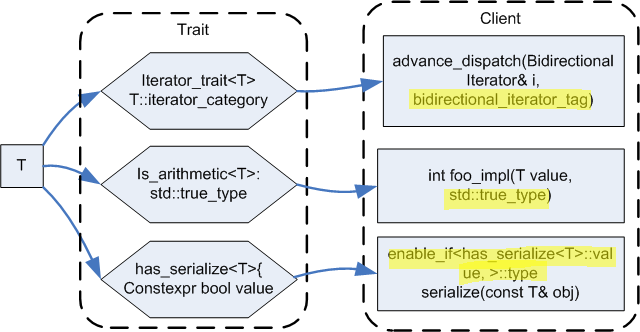
\includegraphics[scale=0.9]{pics/tag_dispatch.png}
\end{center}

	\item For type\_trait side, we introduced two main methods. In "SFINAE(Type deduct) to build trait" section, we use these two methods to implement \texttt{hasSerialize}. After C++ 14, we recommend to use \texttt{void\_t} method. But after C++ 20, we strongly recommend to use \textbf{concept}. On the other side, as a client, we mainly use \texttt{enable\_if} and tag dispatch. But after C++17, we strongly recommend use \texttt{if constexpr}.
	
\end{itemize}

\section{class template}
\subsection{template class and inheritance}
\begin{itemize}

	\item Non-Template class Derived from Template Base class specification
\begin{lstlisting}[numbers=none]
class u8toU16 : public 
		std::codecvt<wchar_t, char, std::mbstate_t>{
	...
};
\end{lstlisting}

	\item Template class Deriving from the non-template class.
\begin{lstlisting}[numbers=none]
class Base
	
template<typename T>
class Derived: public Base
\end{lstlisting}	
	
	\item template class can be used as base class and used as a component class. So we can inherit from a template class.
    \begin{enumerate}
        \item A basic example
\begin{lstlisting}[numbers=none]
template< typename Type>
class SpecialStack: public Stack<Type>{
	Array<Type> array;
}
\end{lstlisting}	
	
        \item If an enum is used by several member functions of the \texttt{std::codecvt} template class, and does not relate to the template parameters. Hence it can exist in a separate base class.
	
\begin{lstlisting}[numbers=none]
template<typename T>
class codecvt_base{
public:
	enum result {ok, partial, error, noconv};
};
\end{lstlisting}
	
	\item You also can extend the derived class by adding another template parameter.
\begin{lstlisting}[numbers=none]
template< typename T>
class Base
	
template<typename T, typename U>
class Derived: public Base<T>
\end{lstlisting}
	
	
	\item Factor parameter-independent code out of templates. Detail can be found in effective item 44. That is to avoid code bloating.
\begin{lstlisting}[frame=single, language=c++]
template<typename T> // size-independent base class for
class SquareMatrixBase { // square matrices
protected:
	...
	void invert(std::size_t matrixSize); //invert matrix of the given size.
	...
};
	
template<typename T, std::size_t n>
class SquareMatrix: private SquareMatrixBase<T> {
private:
	using SquareMatrixBase<T>::invert; 
public:
	...
	void invert() { invert(n); }  //make inline call to base class
	}; // version of invert
\end{lstlisting}
\begin{description}
	\item[Line 12:] make base class version of invert visible in this class; see Items 33 and 43
\end{description}

	
	\item We can derive from a specializing the base class.
\begin{lstlisting}[numbers=none]
template< typename T>
class Base
	
template<typename T>
class Derived: public Base<int>
\end{lstlisting}
\end{enumerate}

\item Parameterized inheritance.
	\begin{enumerate}
	\item Basic example 
\begin{lstlisting}[numbers=none]
template<typename T>
class Derived: public T
\end{lstlisting}
	
	\item \textbf{Two famous idioms are Mixin and Policy, can be found below sections. In this chapter, we only focus syntactic level, not semantic level.}

	\end{enumerate}

\item It can be used as private inheritance. An example can be found in policy section. 

\item Public inheritance. A good introduction can be found in "modern c++ design" first chapter, about creator template class.\textbf{public inheritance means the derived class want to expose the public interface in base class}

\item Public inheritance will expose interface to outside, just like Create() function. private inheritance just implement it. 

\begin{lstlisting}[numbers=none]
template <class T>
struct OpNewCreator{
	static T* Create(){
		return new T;
	}
};
template <class T>
struct MallocCreator{
	static T* Create(){
		void* buf = std::malloc(sizeof(T));
		if (!buf) return 0;
		return new(buf) T;
	}
}; 
// Library code
template <class CreationPolicy>
class WidgetManager : public CreationPolicy{
...
}; 
// Application code
typedef WidgetManager< OpNewCreator<Widget> > MyWidgetMgr; 
\end{lstlisting}

    \item Private inheritance is not the first choice, but the last choice For above example, you don't need private inheritance, you can use previous section "Templates Parameterized by independent class". It's much clear. If policy class has protect member function which we want to use, at this time. private inheritance is our last choice. 

\end{itemize}

\subsection{template and friend}
\begin{itemize}
	\item You can have: 1) friend class, 2) friend function, 3) friend template. At the same time, they can be bound or non-bound. If it's bound, you can find host class parameter T in the friend declaration. 
	
	\item  There are three different kinds for a template class:1) Non-template friend, 2) Bound-template, 3) Unbound-template.


\begin{lstlisting}
template<typename T>
class HasFriend{
	friend void counts();
}
\end{lstlisting}
\begin{description}
	\item[Line 3:] Non-template friend function \texttt{counts()}, The counts is not invoked by an HasFriend obj and has not object parameters.  If counts want to access a HasFriend object, It can access a global one, and use a global pointer to access non-global object.
\end{description}
	
	\item Bound-template friend function. You need to define explicit specialization for the friends you plan to use. Why, because \textbf{1)reports is not template function. 2) reports is not function defintion, 3) report is just function declaration.}
	
\begin{lstlisting}[frame=single, language=c++]
template<typename T>
class HasFriend{
	friend void reports(HasFriend<T> &);
}
	
void reports(HasFriend<int> &hf){
	cout <<hf.item<<endl;
}
void reports(HasFriend<short> &hf){..}
\end{lstlisting}
\begin{description}
	\item[Line 6 to 9:] explicit specialization for the type you plan to use.
\end{description}
	
	\item A better bound-template, reports has <> after it.  and you don't need redefine reports many time like previous codes.\textbf{reports is a template function here. You can think that is a implicit instantiations. }
\begin{lstlisting}[frame=single, language=c++]
template<typename T>
void reports(T &hf){
	cout <<hf.item<<endl;
}

template<typename TT>
class HasFriend{
	friend void reports<>(HasFriend<TT> &);
}
\end{lstlisting}
\begin{description}
	\item[Line 8:] It has <> after reports function name. that is a implicit instantiations.
\end{description}

	\item Non-bound friend template.
\begin{lstlisting}[frame=single, language=c++]
template<typename T>
class ManyFriend{
private:
	item;
	
	template<typename C, typename D>
	friend void show2(C& , D&);
};
	
template <typename C, typename D> void show2(c& c, D& d){
	cout<<c.item<<d.item<<endl;
}
	
ManyFriend<int> mi;
ManyFriend<double>md;
show2(mi,md);
\end{lstlisting}
	
	\item Difference between bound and non-bound:
	
	\begin{enumerate}
		\item bound friend is specialization of template function, so It has <> after the function name.
		
		\item non-bound template use different typename, such as C and D in previous example, and it also use template keyword
		
		\item bound template will produce more function implementation , but non-bound template will only produce ONE function implementation.
	\end{enumerate}
\end{itemize}

\section{template common idiom}

\subsection{policy, mixin and CRTP}
These three patterns are associated, so I put them together. 

\subsubsection{policy}
\begin{itemize}
	
	\item The Policy class can be thought as an optional of multi-inheritance. 
	
\begin{lstlisting}[numbers=none]
template <typename OutputPolicy, typename LanguagePolicy>
class HelloWorld : private 
          OutputPolicy, private LanguagePolicy{
public:
	void run() const{
		// Two policy methods
		print(message());
	}
};
	
class OutputPolicyWriteToCout{
protected:
	template<typename MessageType>
	void print(MessageType const &message) const{
		std::cout << message << std::endl;
	}
};
	
class LanguagePolicyEnglish{
protected:
	std::string message() const{
		return "Hello, World!";
	}
};
	
class LanguagePolicyGerman{
protected:
	std::string message() const{
		return "Hallo Welt!";
	}
};
\end{lstlisting}
\begin{description}
    \item[Source code] Why do we use private inheritance here? Because we don't want to expose \texttt{print} and \texttt{message} methods. We just want to use it. So we use private inheritance here.
\end{description}
\item Client code is below:
\begin{lstlisting}[numbers=none]
int main(){
	/* Example 1 */
	typedef HelloWorld<OutputPolicyWriteToCout, 
	     LanguagePolicyEnglish> HelloWorldEnglish;
	
	HelloWorldEnglish hello_world;
	hello_world.run(); // prints "Hello, World!"
	
	/* uses another language policy */
	typedef HelloWorld<OutputPolicyWriteToCout, 
	     LanguagePolicyGerman> HelloWorldGerman;
	
	HelloWorldGerman hello_world2;
	hello_world2.run(); // prints "Hallo Welt!"
}
\end{lstlisting}
	

		\item If this polymorphism can be known at compile time, we can use "static polymorphism". Use template parameter inject a class with static method. They can be inline and without any runtime overhead. 
\begin{lstlisting}[frame=single, language=c++]
// char_traits::eq
#include <iostream>   // std::cout
#include <string>     // std::char_traits
#include <cctype>     // std::tolower
#include <cstddef>    // std::size_t
	
// traits with case-insensitive eq:
struct custom_traits: std::char_traits<char> {
	static bool eq (char c, char d) { 
	return std::tolower(c)==std::tolower(d); 
}
	
static const char* find (const char* s, std::size_t n, char c)
	{ while( n-- && (!eq(*s,c)) ) ++s; return s; }
};
	
std::basic_string<char,custom_traits> str ("Test");
std::cout<< "found at position" <<str.find('t') ;
\end{lstlisting}
\begin{description}
	\item[Line 13:] some (non-conforming) implementations of \texttt{basic\_string::find} call this instead of eq:
\end{description}

	
	\item This kind of examples can be found a lot in the STL, most of time by a kind of functor. Basic idea is the same.
	
	\item All above technologies are part of generic programming. A good and more example about generic programming examples can be found in "Modern C++ design" a book. The first chapter introduce policy pattern. The second chapter introduce a lot of ways to manage Type information at compile time. 
	
\end{itemize}

\subsubsection{Mixin}
\begin{itemize}
	
	\item \textbf{Mixin refers to the following idiom - a template class that is parameterized on its base class.} Here Mixin classes are template classes that define a generic behaviour, and are designed to inherit from the type you wish to plug their functionality onto.
	
	\item For example, \texttt{RepeatPrint} is Mixin class, T is the type you wish to plug their functionality onto.
\begin{lstlisting}[numbers=none]
template<typename T>
class RepeatPrint : T{
	explicit RepeatPrint(T const& printable) : T(printable) {}
	void repeat(unsigned int n) const{
		while (n-- > 0){
			this->print(); 
			//Make sure printable has print method
		}
	}
};
\end{lstlisting}
	
	\item Supposing that we have an existing type which has print method.
\begin{lstlisting}[numbers=none]
class Name{
public:
	Name(std::string firstName, std::string lastName)
	: firstName_(std::move(firstName))
	, lastName_(std::move(lastName)) {}
	
	void print() const{
		std::cout << lastName_ << ", " << firstName_ << '\n';
	}
	
private:
	std::string firstName_, lastname;
};
\end{lstlisting}
	
	\item We can use it two ways:
\begin{lstlisting}[numbers=none]
//method 1, we use object generator pattern
template<typename T>
RepeatPrint<T> rpGen(T const& printable){
	return RepeatPrint<T>(printable);
}
Name ned("Eddard", "Stark");    
rpGen(ned).repeat(10);

\\method 2, we need to specify type explicitly
RepeatPrint<Name> rp(ned);
rp.repeat(10)
\end{lstlisting}

\end{itemize}


\subsubsection{CRTP}
\begin{itemize}
	\item The basic syntax is Templates Parameterised by a Derived Class.
	
\begin{lstlisting}[numbers=none]
template <class T> 
struct Base{
	void interface(){
		// ...
		static_cast<T*>(this)->implementation();
		// ...
	}
	
	static void static_func(){
		// ...
		T::static_sub_func();
		// ...
	}
};
	
struct Derived : Base<Derived>{
	void implementation();
	static void static_sub_func();
};
\end{lstlisting}
	
	\item A easy way of "call back" is function pointer, but it can't be used inline. so There is efficiency problem. 
	
	\item You can use inheritance, It's runtime polymorphism, and has some runtime overhead. 
	
	\item There are two common usages from CRTP:
	\begin{enumerate}
		\item Static polymorphism. It avoids runtime polymorphism cost. 
\begin{lstlisting}[numbers=none]
template <typename T>
class Amount{
	public:
	double getValue() const {
		return static_cast<T const&>(*this).getValue();
	}
};

class Constant42 : public Amount<Constant42>{
public:
	double getValue() const {return 42;}
};

template<typename T>
void print(Amount<T> const& amount){
	//use base class reference
	std::cout << amount.getValue() << '\n';
}

Constant42 c42;
print(c42);
\end{lstlisting}

\item Adding Functionality.

\begin{lstlisting}[numbers=none]
template <typename T>
struct counter{
	static int objects_created;
	counter(){ ++objects_created;}
};

template <typename T> 
int counter<T>::objects_created{0};

class X : counter<X>{
	// ...
};

X x;
cout<<X::objects_created<<endl;
\end{lstlisting}
\begin{description}
	\item[Line 8:] That is initializing statement. make objects\_created equal 0. 
\end{description}
	\end{enumerate}

\item Below is example template class with CRTP. In the below source code, yan\_vect is the template class. Compared with \texttt{class Constant42} in the previous source code, previous one is non-template class. 
\begin{lstlisting}
template<typename T>
class Base{
public:
	int DoubleSum(){
		return static_cast <T &>(*this).sum()*2;
	}    
};

template<typename T>
struct yan_vect :public Base<yan_vect<T> >{
	yan_vect(int num, T v){ 
		for (int i = 0 ;i<num; i++)
			a[i] = v;
		num_ = num;
	}
	T sum(){
		T result{};
		for (int i = 0 ;i<num_; i++)
			result += a[i];
		return result;
	}
T a[10];
int num_;
};

template<typename T>
void fun(Base<T>& bt){
	cout<<bt.DoubleSum()<<endl;
}

int main(){
	yan_vect<int> vi = {5,2};
	yan_vect<float> vf = {5,1.2};
	fun(vi);
	fun(vf);
}
\end{lstlisting}

\item CRTP patten with template template class, you can see the \texttt{class Base} has template template argument. The below is syntax demo. This pattern doesn't use very widely, I just found on practical usage. please google "An Implementation Helper For The Curiously Recurring Template Pattern"

\begin{lstlisting}
template<typename T, template< typename > class child>
class Base{
	public:
	int DoubleSum(){
		return static_cast <child<T> &>(*this).sum()*2;
	}    
};

template<typename T>
struct yan_vect :public Base<T, yan_vect>{
	yan_vect(int num, T v){ 
		for (int i = 0 ;i<num; i++)
		a[i] = v;
		num_ = num;
	}
	T sum(){
		T result{};
		for (int i = 0 ;i<num_; i++)
		result += a[i];
		return result;
	}
	T a[10];
	int num_;
};

template<typename T >
void fun(Base<T, yan_vect >& bt){
	cout<<bt.DoubleSum()<<endl;
}

int main(){
	yan_vect<int> vi = {5,2};
	yan_vect<float> vf = {5,1.2};
	fun(vi);
	fun(vf);
}
\end{lstlisting}
\item For CTRP: 1) impacts the definition of the existing class, because it has to inherit from the CRTP;2) client code uses the original class directly and benefits from its augmented functionalities.

\item For Mixin class, 1) leaves the original class unchanged. 2) client code doesn’t use the original class directly, it needs to wrap it into the mixin to use the augmented functionality. 3) inherits from a the original class even if it doesn’t have a virtual destructor. This is ok unless the mixin class is deleted polymorphically through a pointer to the original class.

\end{itemize}

\subsubsection{A practical example}
\begin{itemize}
	\item  Consider that there is a Task Manager framework. It is expected that there will be some common bits of functionality that should be reused across task implementations. I have selected task execution timing and logging of start and completion messages to serve as examples. We use six different ways to implement it.
	
	\item method 1, use Mixin
	\begin{enumerate}
		
		\item The function name (Execute) can be different. Here, we use the same name because we can recursive use it. such as: \texttt{LoggingTask< TimingTask< MyTask > > Task;}
		
		\item A detail can be found "C++ Mixins - Reuse through inheritance is good... when done the right way" and "Mixin Classes: The Yang of the CRTP"
		
\begin{lstlisting}[numbers=none]
class MyTask{
public:
void Execute(){
	std::cout << "task is executed" << std::endl;
	}
};
		
template< class T >
class LoggingTask : public T{
public:
	explicit LoggingTask(T const& t) : T(t) {}
			
	void Execute(){
		std::cout << "LOG: The task is starting - " ;
		T::Execute(); 
		std::cout << "LOG: The task has completed - " ;
	}
};
		
LoggingTask<  MyTask  > t;
t.Execute();
\end{lstlisting}
		
		\item if you have a MyTask value, you can build a helper function to build Mixin class 
\begin{lstlisting}[numbers=none]
template<typename Task>
LogTask<Task> getLogTask(Task const& task){
	//Call the below explicit constructor in LogTask class
	return LogTask<Task>(task);
}
		
getLogTask(task).Execute //with log funcitons
\end{lstlisting}
		
	\end{enumerate}
	
	\item method 2, use CRTP
	\begin{enumerate}
		\item Use base class extend and reuse function(Execute\_imp)
		\item Expose Execute interface to client by base class 
		\item Client can directly use MyTask.
	\end{enumerate}
\begin{lstlisting}[numbers=none]
template< class Task >
class LoggingTask {
public:
	void Execute(){
		std::cout << "LOG: The task is starting - " ;
		static_cast<Task const&>(*this).Execute_imp();
		std::cout << "LOG: The task has completed - " ;
	}
};
	
class MyTask:public LoggingTask<MyTask> {
public:
	void Execute_imp(){
		std::cout << ".task is executed..." ;
	}
};
	
MyTask t;
t.Execute();
\end{lstlisting}
	
	\item method 3, template Method
	\begin{enumerate}
		\item No template, just use run time polymorphism
		\item Base class define a basic flow of action, some part of action is override in the Child class, That is Template Method pattern in design pattern.
	\end{enumerate}
\begin{lstlisting}[numbers=none]
class BaseLoggingTask{
public:
	void Execute(){
		std::cout << "LOG: The task is starting - " ;
		OnExecute();
		std::cout << "LOG: The task has completed - ";
	}
	virtual void OnExecute() = 0;
};
	
// Concrete Task implementation that 
//reuses the logging code of the BaseLoggingTask
class MyTask : public BaseLoggingTask{
public:
	virtual void OnExecute(){
		std::cout << "task is executed..." << std::endl;
	}
};
	\end{lstlisting}
	
	\item method 4, command pattern
	\begin{enumerate}
		\item That is command pattern.
		\item For Logging Task, you can see the class \textbf{includes and derived from ITask at the same time}. 
		\item Command pattern is illustrated by below figure:
		\newline
		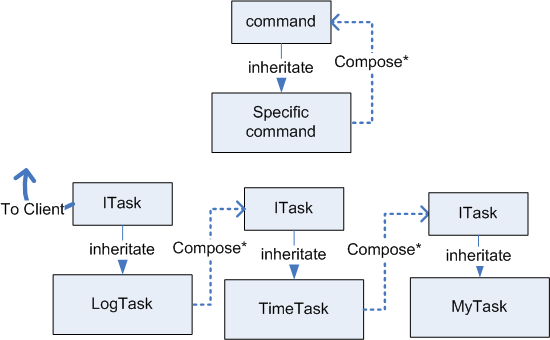
\includegraphics[scale=1.1]{pics/command.png}
	\end{enumerate}
\begin{lstlisting}[numbers=none]
class LoggingTask : public ITask{
	ITask* task_;
public:
	LoggingTask( ITask* task ) : task_( task ){ }
	
	~LoggingTask(){
	delete task_;
}
	
	virtual void Execute(){
		std::cout << "LOG: The task is starting - " 
		          << GetName().c_str() << std::endl;
		if( task_ ) task_->Execute();
		std::cout << "LOG: The task has completed - " 
		         << GetName().c_str() << std::endl;
	}
};
	
class MyTask : public ITask{
public:
	virtual void Execute(){
		std::cout << ".task is executed..." ;
	}
};
	
ITask* t = new LoggingTask(new MyTask()) ;
t->Execute();
\end{lstlisting}
	
	
	\item method 5, mixin many mixin

\begin{lstlisting}[numbers=none]
template< class T >
class LoggingTask : public T{
	public:
	void Execute(){
		std::cout << "LOG: The task is starting - " 
		         << GetName().c_str() << std::endl;
		T::Execute();
		std::cout << "LOG: The task has completed - " 
		         << GetName().c_str() << std::endl;
	}
};
	
template< class T >
class TimingTask : public T{
	Timer timer_;
public:
	void Execute(){
		timer_.Reset();
		T::Execute();
		double t = timer_.GetElapsedTimeSecs();
		std::cout << "Task Duration: " << t <<;
	}
};
	
class MyTask{
	public:
	void Execute(){
		std::cout << "task is executed..." ;
	}
};
	
tyedef LoggingTask< TimingTask< MyTask > > Task;
Task t4;
t4.Execute();
\end{lstlisting}

		\item method 6, policy base
\begin{lstlisting}[numbers=none]
class coutLog{
	void beginLog(){
		cout<< "LOG: The task is starting - " <<endl
	}
	
	void endLog(){
		cout << "LOG: The task has completed - "
	}
}
	
template<typename LogPolicy, typename TimePolicy>
class Task: private LogPolicy, TimePolicy{
	void Execute(){
		beginLog();
		beginTime();
		std::cout << "This is where the task is executed";
		endTime();
		endLog();}
\end{lstlisting}
	
	\item summary:
	\begin{enumerate}
		\item Policy can be used when you log and time funciton change a lot
		\item Mixin and command can be compose the multi-actions
		\item template is more efficient than inheritance. 
		\item Command pattern can also be thought as composite pattern.
		\item Mixin will not change current class, but CRTP change the current class interface.
	\end{enumerate}
	
\end{itemize}

\subsubsection{summary}
\begin{itemize}
	\item Basic idea is illustrated below: This figure is very important and worth digging in and understand more. Fox example, for \texttt{Class Foo: T}, we can call it as policy idiom if we focus Foo. We can also call it as Mixin idiom if we focus on T. In Mixin idiom, Foo just want to add some functionality into T. CRTP has the same distinguishing idea. If we focus on parent class, we want to use static dynamic. If we focus on child class, we just want to add some functionality to child class. A typical usage for this idea is \texttt{std::enable\_shared\_from\_this}. 

		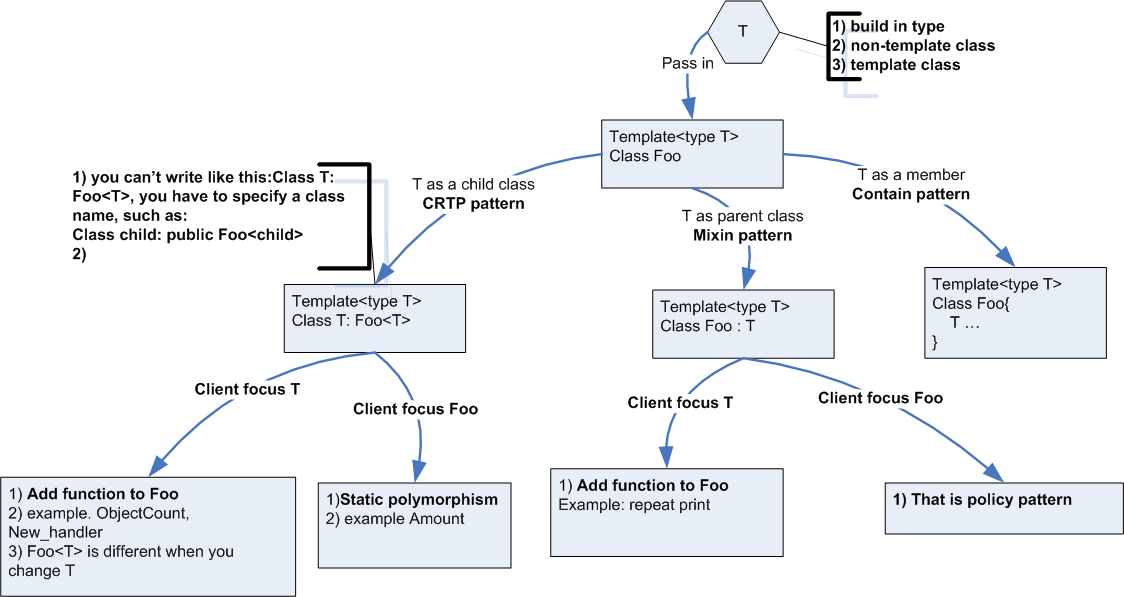
\includegraphics[width=0.9\linewidth]{pics/mixin.png}
		
	\item For Contain pattern, we can use template template parameter.
	
		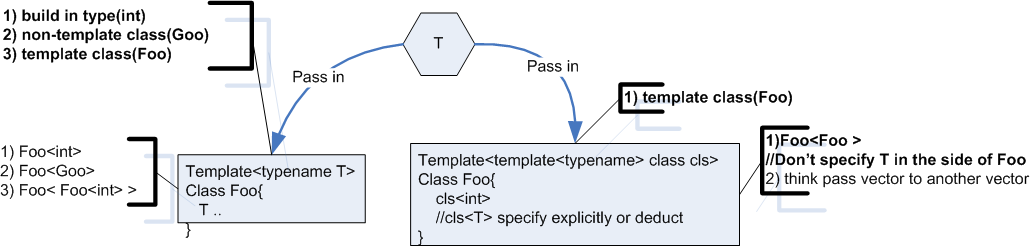
\includegraphics[width=0.9\linewidth]{pics/mixin_tt.png}
		
	\item For CRTP pattern, we can use template template parameter.
	
		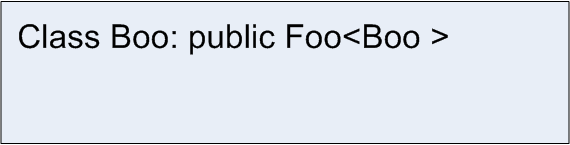
\includegraphics[width=0.9\linewidth]{pics/crtp_tt.png}

\end{itemize}


\subsection{type erasure and concept}

\subsubsection{type erasure}
\begin{itemize}
\item When you implement type erasure, it always starts with making a list of the things you want to be able to do with your type-erased object - call it, destroy it, copy it, and so on. For example, \textbf{A std::function affords copying and calling}. A \texttt{std::any} affords copying, but not calling. A \texttt{unique\_function} affords calling and moving, but not copying.

\item Each accordance in your requirement list turns into a virtual member function of\texttt{ AbstractWhatever}, which will be overridden by \texttt{WrappingWhatever<T>} appropriately for T. Finally, the top-level Whatever will store a\texttt{ unique\_ptr<AbstractWhatever> ptr\_} (and/or an SBO buffer), and provide a clean non-virtual interface implemented completely in terms of calling virtual member functions on \texttt{*ptr\_}. An implementation design is illustrated by below code and picture:



\item An implementation source code is below:
\begin{lstlisting}[frame=single, language=c++]
struct Plus1 {
	int call(int x) const { return x+1; }
};

struct AbstractCallback {
	virtual int call(int) const = 0;
	virtual ~AbstractCallback() = default;
};

template<class T>
struct WrappingCallback : AbstractCallback {
	T cb_;
	explicit WrappingCallback(T &&cb) 
	                : cb_(std::move(cb)) {}
	                
	int call(int x) const override 
	          { return cb_(x); }
};

struct Callback {
std::unique_ptr<AbstractCallback> ptr_;

template<class T>
Callback(T t) {
	ptr_ = std::make_unique<WrappingCallback<T>>
	                            (std::move(t));
}
int operator()(int x) const {
	return ptr_->call(x);
}
};

int run_twice(const Callback& callback) {
	return callback(1) + callback(1);
}

int y = run_twice([](int x) { return x+1; });
assert(y == 4);
\end{lstlisting}
\begin{center}
	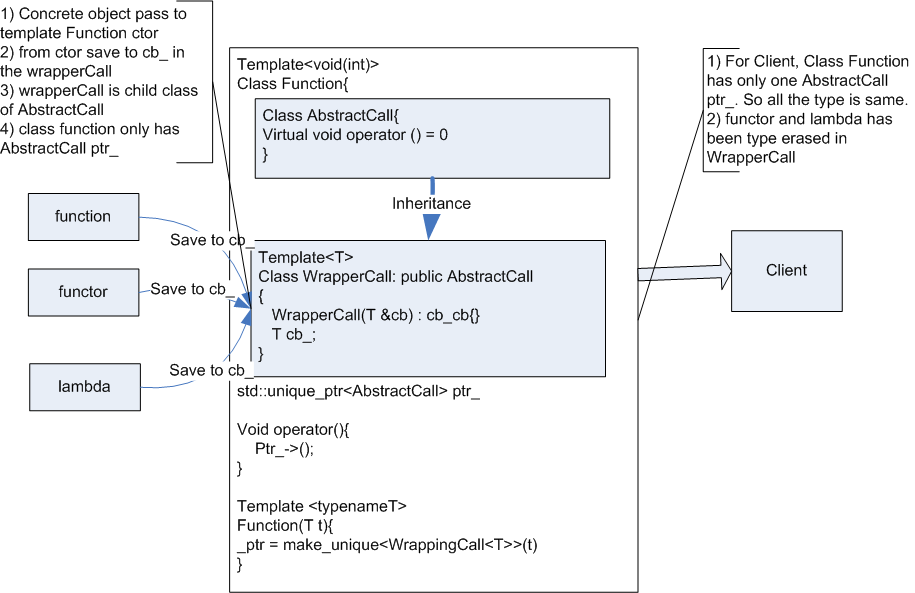
\includegraphics[scale=0.9]{pics/function1.png}
\end{center}

\item A good article is "What is Type Erasure" A detail implementation can be found in:\\ \verb|http://blog.bitfoc.us/p/525|
\end{itemize}

\chapter{STL}
\section{Basic}
\subsection{Four components in STL}
\begin{itemize}
\item When you use STL library, \textbf{always include the proper headers.} You should include corresponding header files when you use container and algorithms.
\begin{enumerate}

\item All the algorithms are declared in <algorithm>. \texttt{inner\_product}, \texttt{adjacent\_difference}, \texttt{partial\_sum} and \texttt{accumulate} are in the <numeric>.

\item Special kinds of iterators , including \texttt{istream\_iterators} are in the <iterator>

\item Standard functors, eg \texttt{less<T>} and functor adapter \texttt{not1}, \texttt{bind2nd} are declared in <functional>. They are not recommended to use in C++11. Because C++ 11 introduces \textbf{function} and \textbf{bind} template.

\end{enumerate}

\item There are \textbf{Containers, iterators, functions objects, and algorithms} in STL. \textbf{Use functor customize algorithms, then apply algorithm on Containers by iterators.} Such as algorithms: \texttt{std::find}, you can input two Iterators into it.  \texttt{std::find} doesn't care what container which he will look for a value in it.  \texttt{std::find} in fact is a template function, it doesn't use inheritance to make generic programming, but use template.  

\begin{lstlisting}[frame=single, language=c++]
struct Sum{
    Sum(): sum{0} { }
    void operator()(int n) { sum += n; }
    int sum;
};

std::vector<int> nums{3, 4, 2, 8, 15, 267};
std::for_each(nums.begin(), nums.end(), [](int &n){ n++; }) //lambda syntax
Sum s = std::for_each(nums.begin(), nums.end(), Sum());  //return Sum struct
cout<<s.sum<<endl;
\end{lstlisting}

\end{itemize}

\subsection{common used design idioms in std}
\begin{itemize}
	\item Some common used idioms in std:
	\begin{enumerate}
		\item concept
		\item traits
		\item tag dispatching
		\item adapters
		\item type generators
		\item object generators
		\item policy classes
	\end{enumerate}
	
	\item A \textbf{concept} is a set of requirements consisting of valid expressions, associated types, invariant, and complexity guarantees. A type that satisfies the requirements is said to \textbf{model} the concept. A concept can extend the requirements of another concept, which is called \textbf{refinement}.

\begin{description}
	\item[Valid Expressions] are C++ expressions which must compile successfully for the objects involved in the expression to be considered models of the concept. For example, an \texttt{Iterator x} is expected to support the expressions \texttt{++x} and \texttt{*x}.
	
	\item[Associated Types] are types that are related to the modeling type in that they participate in one or more of the valid expressions. Typically associated types can be accessed either through typedefs nested within a class definition for the modeling type, or they are accessed through a traits class. For example, an iterator's value type is associated with the iterator through \texttt{std::iterator\_traits}
	
	\item[Invariants] are run-time characteristics of the objects that must always be true, that is, the functions involving the objects must preserve these characteristics. The invariants often take the form of pre-conditions and post-conditions. For example, Forard iterator is copied, the copy and original must comare equal.
	
	\item[Complexity Guarantees] are maximum limits on how long the execution of one of the valid expressions will take, or how much of various resources its computation will use.
\end{description}

\item An adaptor is a class template which builds on another type or types to provide a new interface or behavioral variant. Examples of standard adaptors are \texttt{std::reverse\_iterator}, which adapts an iterator type by reversing its motion upon increment/decrement, and \texttt{std::stack} , which adapts a container to provide a simple stack interface.
	
\item An object generator is a function template whose only purpose is to construct a new object out of its arguments. Think of it as a kind of \textbf{generic constructor}. An object generator may be more useful than a plain constructor when the exact type to be generated is difficult or impossible to express and the result of the generator can be passed directly to a function rather than stored in a variable. Most Boost object generators are named with the prefix "make\_", after \texttt{std::make\_pair(const T\&, const U\&)}.
	
\end{itemize}


\section{Container}

\subsection{Basic knowledge}
\begin{itemize}

\item For all container, \textbf{Copy in, Copy out}. In C++11, you can use \texttt{emplace\_back} to build object directly on the \texttt{vector} to avoid copy.
\begin{lstlisting}[numbers=none]
int j = 10;
vector<int> vc;
vc.push_back(j); // not j, but copy of j to vc

int i = vc.pop_back(); 
i = -99 // when you modify i, not effect on vc
\end{lstlisting}

\item Even copy in, copy out. \texttt{vector} is more flexible than array in C language. Because it use heap memory, if you want to use stack memory, you can use \texttt{std::array}.
\begin{lstlisting}[numbers=none]
Foo farray[50]; //default constructor has been called 50 times.
Foo *parray = new Foo[50]; 
//Same, constructor will be called 50 times.

vector<Foo> fvc; // no default constructor has been called.
fvc.reserve(50);
\end{lstlisting}

\item \textbf{Anytime you want to write new [..] just for allocate dynamic array, using a \texttt{vector} or string instead, and using reserve() to allocate enough space.}


\item Copy in and copy out can cause efficient problem. Furthermore, when you inserting a derived class object into a container of base class objects is always error (slicing error). In order to fight this problem, you can use container of pointer. But it will cause resource leaking problem if you forget or an exception is thrown. So a better choice is to use smart pointer. But don't use \texttt{auto\_ptr} in any container, It's prohibited in c++, and produce a compiler error, see effective stl item 8.

\item All container is not thread-safe. It's your duty to make it thread-safe, and thread-safe is OS dependent. Detail can be seen effective STL item 12.
\begin{lstlisting}[numbers=none]
getMutexFor(v);
// do something on v.
releaseMutexFor(v);
\end{lstlisting}

\item There are three kinds of for-loop container syntax; \textbf{for\_each is a tool for raising the level of abstraction of a range-based for loop}. A good article can google " Why You Should Use \texttt{std::for\_each} over Range-based For Loops"
\begin{lstlisting}
for(auto it = con.begin(), itend = con.end();
         it !=itend ; ++it){
   foo(*it);
}

for_each(con.begin(), con.end(), [](Element& e){.})
for_each(begin(c),end(c), fun1); //good style, but it also adds begin and end
range::for_each(c,fun1);  //best style, support in C++20

for(auto & e : con){
   foo(e);
}
\end{lstlisting}
\begin{description}
\item[Line 6:] showing the inside of the lambda within the call to \texttt{for\_each} is not good style.
\end{description}


	\item With help of allocator, container can use this to do some optimization. For example, for POD, you don't need to all constructor. For small object, you can put them in the memory pool etc.  More detail can be found "source code of STL". In fact, allocator can be customized, two examples can be found in "effective STL". 
	
	\item In one word, we don't need to replace default allocator. allocator is not good design from beginning. It will cause \texttt{vector<int, allocA>} and \texttt{vector<int, allocB>} two different types. 
\end{itemize}


\subsection{Basic classifications}
\subsubsection{structure classification}
\begin{itemize}

\item STL container: sequence container, associative container and container adapter:
\begin{enumerate}
\item sequence: \texttt{vector, list, forward\_list, string,  deque}
\item associative: \texttt{map , multiset , set, multimap, unordered\_map unordered\_set}
\item adapter: \texttt{stack, queue and priority\_queue}.
\end{enumerate}

\begin{figure}[ht]
	\centering
	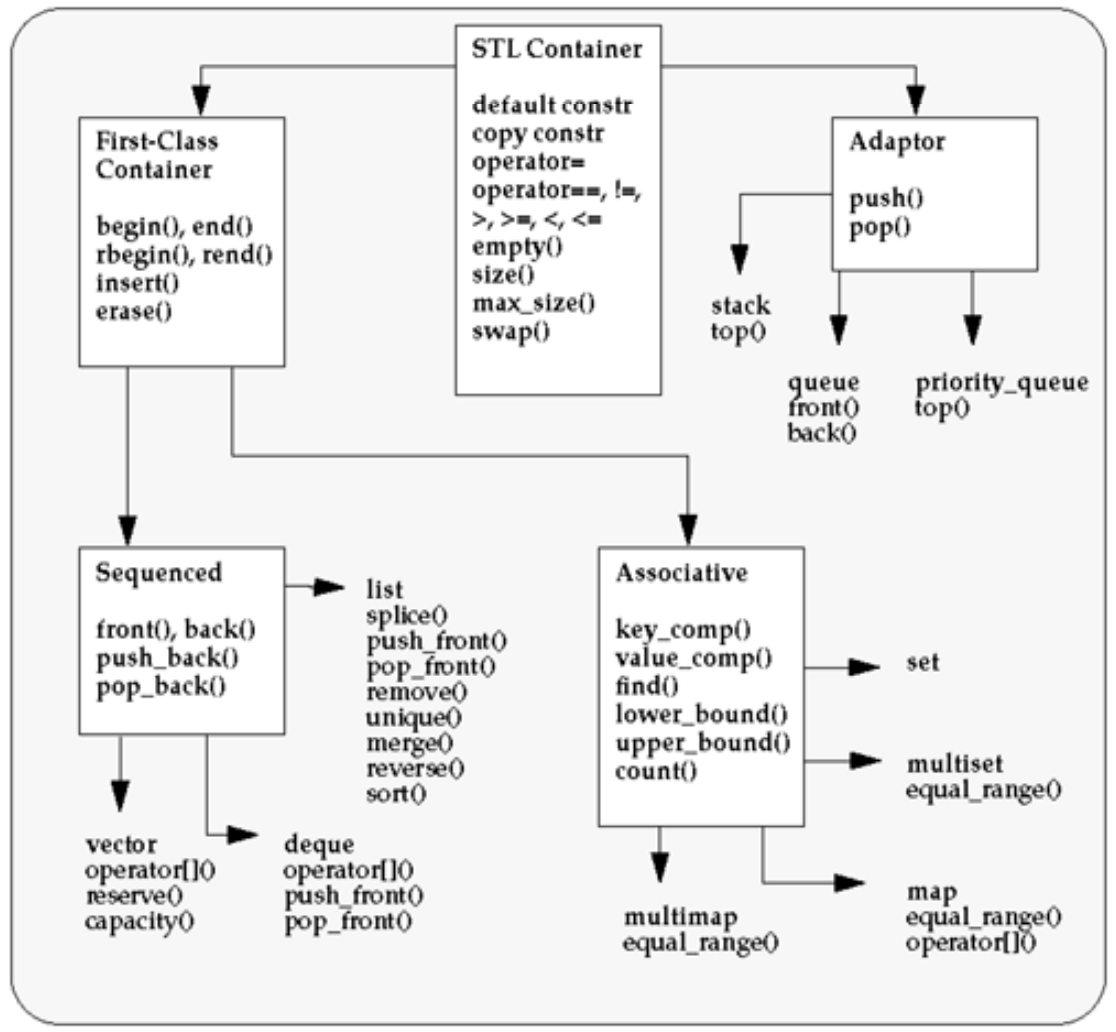
\includegraphics[width=0.7\linewidth]{pics/container.png}
	\label{fig:constexpr}
\end{figure}

\item Dig deeper into STL container.

\begin{enumerate}
	\item \texttt{operator >, >=, ==...} is non member function. 
\begin{lstlisting}
std::vector<int> alice{1, 2, 3};
std::vector<int> bob{7, 8, 9, 10};

bool result = alice > bob;
bool result = alice < bob;
\end{lstlisting}	

\item all container support \texttt{empty()}, \texttt{size()}, \texttt{max\_size()}, and \texttt{swap()}. \texttt{max\_size() }is just theoretical value. (4  functions)

\item First class container includes \texttt{begin()}, \texttt{end()}, \texttt{rbegin()}, \texttt{rend()}. \texttt{insert()} and \texttt{erase()}. (6 functions) \textbf{There are no six functions in adaptor and insert and erase are in very high level.}

\item sequence container support \texttt{pop\_back()}, \texttt{push\_back()},\texttt{front()} and \texttt{back()} (4 functions)
 while associative don't.
 
\item \texttt{vector} supports \texttt{operator[]}, \texttt{list} support \texttt{push\_front} and \texttt{pop\_front}. and \texttt{deque} support both. (3 function.)  By now \texttt{deque} support (4+6+4+3 = 17 functons)\textbf{container(4)--> first container(6)-->sequence container(4)-->deque(3)}

\item \textbf{Associate container doesn't support \texttt{push\_back} and \texttt{pop\_back}, we can only use \texttt{insert} and \texttt{erase} to add or delete element.} Although we can't \texttt{push\_back}, but we can use \texttt{begin} and \texttt{end} on assocaite container to get iterator.

\item \texttt{vector} supports \texttt{reserve()}, \texttt{list} has \texttt{reverse()}(\textbf{not reserve}) and \texttt{splice()}.  \texttt{deque} supports nothing.

\item \texttt{list} support it's own  version \texttt{sort()}, \texttt{remove()}, \texttt{merge()},\texttt{unique()}. For other container, you can use the generic algorithm, Why \texttt{list} has its own? For \texttt{sort()}, \texttt{list} doesn't support random access iterator. For \texttt{merge(), remove()} and \texttt{unique()}. generic algorithm just use copy method, but \texttt{list} has high efficient pointer implementation, So \texttt{list} offer its own version \texttt{merge()}, \texttt{remove()},\texttt{sort()}, \texttt{unique()}.

\item All first class container support \texttt{begin()} and \texttt{end()}. Only sequence containers support \texttt{push\_front()} or \texttt{push\_back()}. \textbf{begin is not equal front, begin can be used for all first class container, but front only be used for sequence container.}

\begin{enumerate}
\item \texttt{begin()} and \texttt{end()} return iterator, and all first container support them, beside adaptor.

\item \texttt{front()} and \texttt{back()} return reference, and all sequenced container support them, \textbf{not associative container.}

\item \texttt{push\_front()} and \texttt{push\_back()} add element, and \texttt{vector} only support \texttt{push\_back()}. \texttt{deque} and \texttt{list} support both.
\end{enumerate}

\item  If you can find same name member functions in container, prefer to use member function than generic algorithm. Such as \texttt{sort, merge, remove, reverse, unique} in \texttt{list}, and \texttt{find, count, low\_bound} in \texttt{set} and \texttt{map}. 

\item Associative containers support their own \texttt{find()}, \texttt{count()},  \texttt{lower\_bound()}, \texttt{upper\_bound()} , \texttt{equal\_range()}. They share the same name with generic algorithm, Don't confuse them. When you deal with associative container, just use container member function, don't use generic algorithm. \textbf{Associative offer log-time lower\_bound, upper\_bound and equal\_range, but generic algorithm just linear time.}


\item \texttt{deque} is the data structure of choice when most insertions and deletions take place at the beginning or at the end of the sequence. It doesn't not guarantee continuity within memory, and higher constant factor cost than vector. One of memory layout is shown in Fig. 9.2.  Although both offer random access to elements and linear-time insertion and removal from middle of a sequence, the \texttt{vector} is faster.  

\begin{figure}[ht]
	\centering
	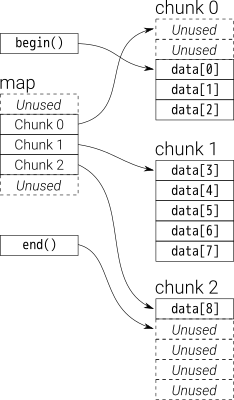
\includegraphics[width=0.2\linewidth]{pics/queue.png}
	\caption{Implementation of deque}
	\label{fig:queue}
\end{figure}


\item Difference between \texttt{vector} and deque:
\begin{enumerate}
\item \texttt{vector} has relocation problem, if \texttt{vector} has 1000, It probably need log(1000) = 10 times relocation. that is a little costly. On the contrary, \texttt{deque} just allocate a new place then insert pointer of new place to pointer map. It's relatively cheap.


\item Elements in a \texttt{deque} are not contiguous in memory; \texttt{vector} elements are guaranteed to be. So if you need to interact with a plain C library that needs contiguous arrays, or if you care (a lot) about spatial locality, then you might prefer vector.

\item For stack and queue default use \texttt{deque} as container inside. Why, because for a large amount of element, \texttt{vector} has relocation problem,
\end{enumerate}


\item All the container adapter support \texttt{push()}, \texttt{pop()}. \texttt{stack} and \texttt{priority\_queue} support \texttt{top()}. queue has \texttt{front and back}. They don't have any iterators.

\item If you want strongly error-safe code, such as transnational semantics for inserting and erasing, or need to minimize iterator invalidation, prefer a node-based container.

\item Using a \texttt{vector} for small \texttt{list} is almost always superior to using \texttt{list}. Even though insertion in the middle of the sequence is a linear-time operation for \texttt{vector} and a constant-time operation for list. \texttt{vector} usually outperforms \texttt{list} because of its better constant factor. \textbf{list's Big-Oh advantage doesn't kick in until data sizes get larger}


\end{enumerate}

\end{itemize}


\subsubsection{memory classification}

\begin{itemize}
\item Another classification of container : \textbf{contiguous-base and node-base.}

\begin{enumerate}
\item \texttt{vector}, \texttt{string}, and \texttt{deque} are contiguous-base.
\item \texttt{list} and \texttt{slist}(linked list), \texttt{set} and \texttt{map}(balanced trees) are node-base.
\end{enumerate}

\item Why we have such classification? 
\begin{enumerate}
\item \textbf{Because all the contiguous-base container has invalidation of iterator(pointer, reference) problem. }

\item \textbf{All the node-base containers only support bidirectional iterators. }

\item \textbf{All the node-base containers don't have reserve() function and need NOT to worry reallocation problem. \texttt{deque} doesn't have \texttt{reserve()} function either }
\end{enumerate}

\item About the iterator invalidation problem,  First, you need to know the invalidation rules below: 
\begin{description}
\item[push and pop]
\texttt{push\_back()} and \texttt{push\_front()} are defined in terms of \texttt{insert()}. Similarly, pop\_back() and pop\_front() are defined in terms of \texttt{erase()}.

\item[Insertion]
\begin{itemize}
\item Sequence containers
		\begin{description}
		\item [vector:] All iterators and references before the point of insertion are unaffected, unless the new container size is greater than the previous capacity (in which case all iterators and references are invalidated)
		
		\item [deque:] All iterators and references are invalidated, unless the inserted member is at an end (front or back) of the \texttt{deque} (in which case all iterators are invalidated, but references to elements are unaffected)
		
		\item [list:] all iterators and references unaffected
		\end{description}

\item Associative containers: \texttt{[multi]\{set,map\}} all iterators and references unaffected

\item Container adapters:  \texttt{stack}, \texttt{queue} and \texttt{priority\_queue}: inherited from underlying container.(Usually, we don't use iterator in \texttt{stack}, \texttt{queue} and \texttt{priority\_queue}. Maybe you don't need to worry about it. )
\end{itemize}

\begin{lstlisting}[frame=single, language=c++, mathescape=true]	
vecArr.insert ( it + 2, 1 , 200 );
it = vecArr.begin(); //Reinitialize the invalidated iterator to the beginning.
\end{lstlisting}

\item[Erasure]
	\begin{itemize}
			\item Sequence containers
					\begin{description}
					\item [vector:] every iterator and reference after the point of erase is invalidated
					
					\item [deque:] all iterators and references are invalidated, unless the erased members are at an end (front or back) of the \texttt{deque} (in which case only iterators and references to the erased members are invalidated). You can see here it is different with inserting in the front. Because deque maybe has a array of pointer as a index table, insert in the front maybe need add a new pointer in the beginning of array of pointer, so it will invalid all the iterator. 
					
					\item [list:] only the iterators and references to the erased element is invalidated
					\end{description}
			
			\item Associative containers: \texttt{[multi]\{set,map\}}: only iterators and references to the erased elements are invalidated
			
			\item Container adaptors: stack, queue and priority\_queue: inherited from underlying container
	\end{itemize}

\begin{lstlisting}[]
auto it = std::find(vecArr.begin(), vecArr.end(), 5);
if(it != vecArr.end())
	vecArr.erase(it);
    //it = vecArr.erase(it);

for(; it != vecArr.end(); it++)//Unpredicted Behavior
 std::cout<<(*it)<<"  "; //Unpredicted Behavior
\end{lstlisting}
\begin{description}
	\item[Line 4:] We can use method illustrated by line 4 to resolve this problem.
	
	\item[Line 6 and 7:]  Now iterator \texttt{it} is invalidated because it still points to old location, which has been deleted.
\end{description}

\item[swap]
no \texttt{swap()} function invalidates any references, pointers, or iterators referring to the elements of the containers being swapped.

\item[Resizing]
\texttt{vector}, \texttt{deque} and \texttt{list} as per insert/erase
\end{description}

\end{itemize}

\subsection{Container Practical Usage}

\subsubsection{Sizes and Capacity}
\begin{itemize}
	\item For container, Call \texttt{empty()} instead of of checking \texttt{size()} against zero. it's very easy to understand it.
	
	\item for vector, \texttt{size()}, \texttt{capacity()} and \texttt{max\_size()} can be seen below: capacity is equal or bigger than size. So if you want to avoid allocate the unnecessary space.  LLVM give a \texttt{SmallVecotr<type, N>} example, you can use \texttt{N} to specify a smaller \texttt{vector} to avoid waste.
\begin{lstlisting}[frame=single, language=c++]
std::vector<int> myvector;
for (int i=0; i<100; i++) myvector.push_back(i);

std::cout << (int) myvector.size() << '\n'; // 100
std::cout  << (int) myvector.capacity() << '\n';//128
std::cout << (int) myvector.max_size() << '\n';//1073741823
\end{lstlisting}	
	
	
	\item Four confused conceptions:
\begin{lstlisting}[frame=single, language=c++]
capacity() //how many CAN hold
size()   //how many are in NOW
resize(n) //initial or fill with default constructor.
reserve(n) //cause the container's capacity() to at lease n.
\end{lstlisting}	
	\begin{description}
		\item[Line 3:] \texttt{resize()} forces the container to change to n, if n is less than \texttt{size()},  object in the end will be lost. if n is greater than \texttt{size()},  default constructor of element will be called. after \texttt{resize(n)}, size will return n. but \texttt{resize} don't change capacity. Pay attention to here.\texttt{ resize} will call default constructor, so maybe there is performance issue here. 
	\end{description}
	
	\item You want to avoid allocation, 1), if you know the number, then use \texttt{reserve}, 2) if you don't know the number, you can reserve maximum space, then you can trim off any excess capacity.  you can use \texttt{shrink\_to\_fit()} function too. 
\begin{lstlisting}[frame=single, language=c++]
vector<class> v1;
v1.reserve(1000); v1.size(); // only 5

vector<class>(v1).swap(v1);

string(s).swap(s) // the same idea behind.
\end{lstlisting}
	\begin{description}
		\item[Line 4:] \texttt{vector<class>(v1)} copy constructor create a temp vector. temp just copy real object, so it's capacity (maybe 8)is small. temp.swap(v1) then temp has 1000 space,  v1 capacity is 8 now. in the end of statement, temp is destroyed.
	\end{description}
	
	\item \texttt{clear} only change size to 0, but will not change capacity

	\item \texttt{resize} and \texttt{reserve} difference.
\begin{lstlisting}[frame=single, language=c++]
	vector<Foo> vcFoo;
	vcFoo.reserve(10); //just allocate space, don't build object.
	vcFoo.resize(10);  // beside alloate space, also build object.
	vcFoo[2] = foo; 
\end{lstlisting}	
	\begin{description}
		\item[Line 3:] will call Foo constructor 10 times.
		\item[Line 4:] will call Foo constructor and assignment 1 times. if we don't call \texttt{resize()} before, \texttt{vcFoo[2] = foo} will fail.
	\end{description}
	
\end{itemize}


\subsubsection{Search in Container}
\begin{itemize}
\item Distinguish among \texttt{count}, \texttt{find}, \texttt{binary\_search}, \texttt{lower\_bound}, \texttt{upper\_bound}, and \texttt{equal\_range}.

\begin{center}
	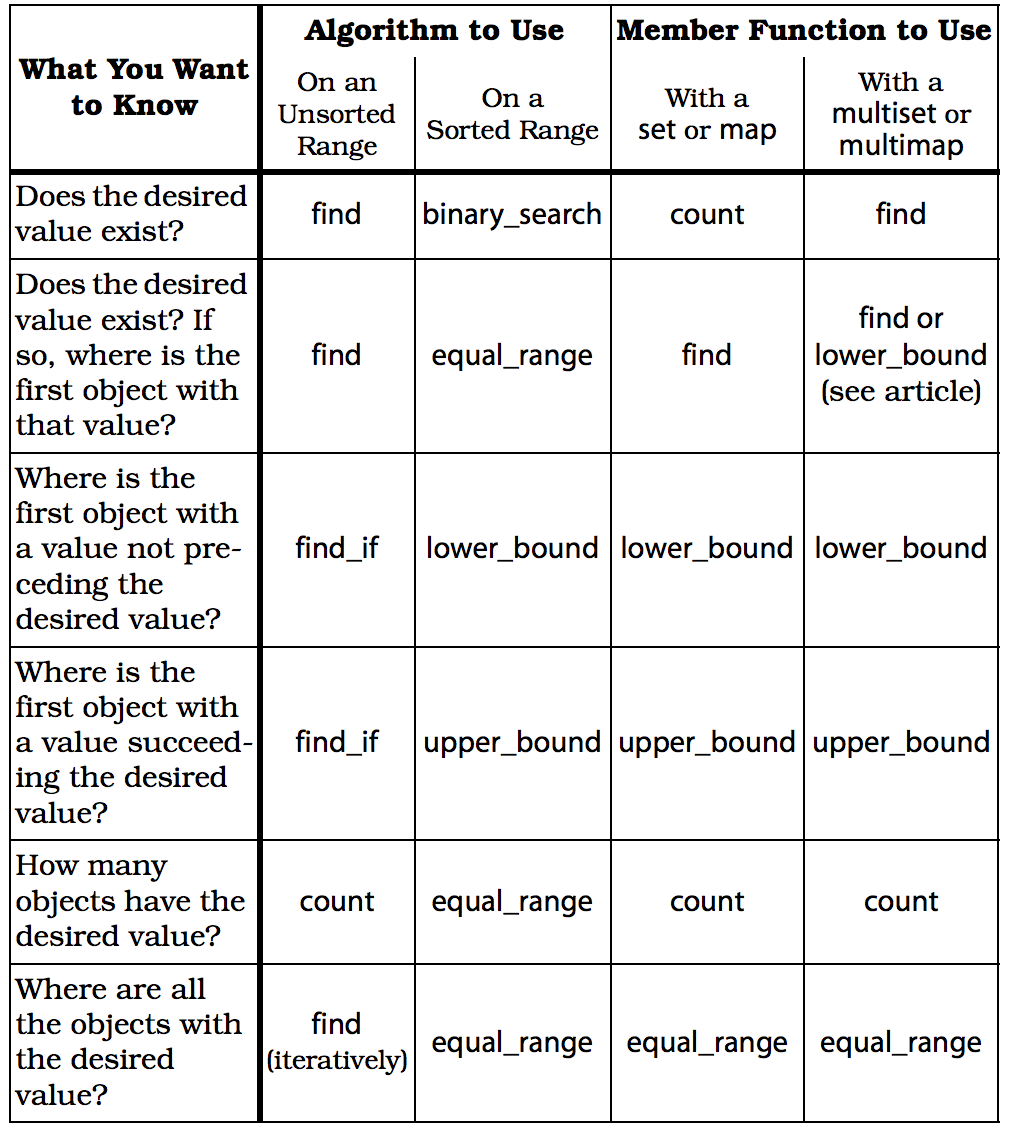
\includegraphics[scale=0.6]{pics/distinguish.png}
\end{center}

\begin{enumerate}
\item \textbf{For unsorted range, just generic find() or find\_if() algorithm or count. return end() iterator if no find element.}

\item \textbf{For sorted range, Only four algorithms: binary\_search, lower\_bound, upper\_bound, and equal\_range. are used on a sorted range.}

\item \textbf{For set or map, It has own version, \texttt{find()}, \texttt{count()} and \texttt{lower\_bound}, \texttt{upper\_bound}, and \texttt{equal\_range}}

\item Don't use generic \texttt{find()} algorithm on a sorted range,  use \texttt{binary\_search()}. binary\_search just return bool, not position.

\item  \texttt{find()} will return match iterator, if no match, it will return end()(for map or set). or last iterator(for generic algorithm). but \texttt{Lower\_bound}  will return a position anyway, match position or insert position(no match).

\item Lower bound: first element that is greater-or-equal. Upper bound: first element that is strictly greater. equal\_range return a pair of (\texttt{lower\_bound}, \texttt{upper\_bound}).

\begin{center}
	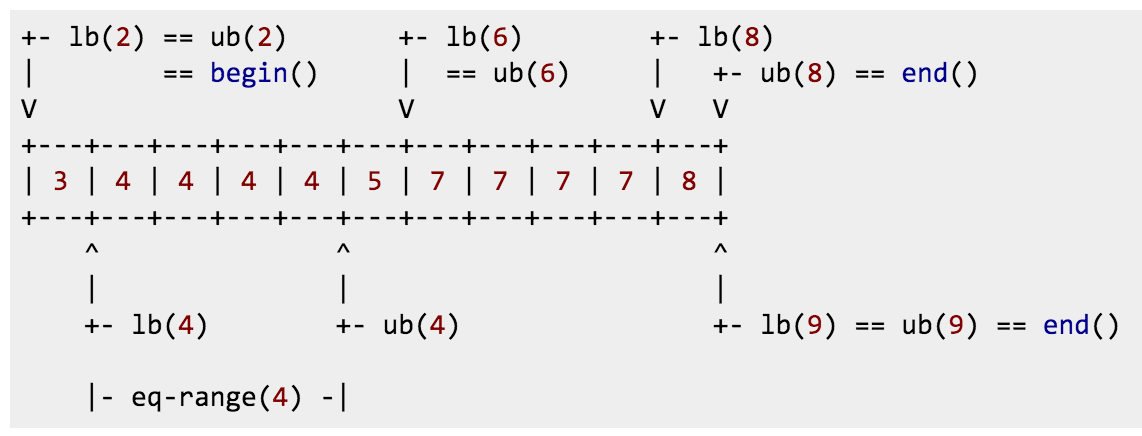
\includegraphics[scale=0.5]{pics/lowerupper.png}
\end{center}


\item \texttt{equal\_range} if two iterators equal, (no found,). if two iterators distance >=1, (find one or more match, can replace \texttt{find()} or \texttt{count()} function.) .
\begin{lstlisting}[frame=single, language=c++]
  std::sort (v.begin(), v.end());
  // 10 10 10 20 20 20 30 30
 auto p =std::equal_range (v.begin(), v.end(), 20);
 for ( auto i = p.first; i != p.second; ++i )
        std::cout << i->name << ' ';

  //or code below:
  if(distance(p.first, p.second)  >=1){
       cout<<" found match"<<endl;
  }
\end{lstlisting}

\end{enumerate}
\end{itemize}


\subsubsection{Range}

\begin{itemize}

\item Copy algorithm usage: 1) copy v2 to v1.  2) it use loop inside.  \textbf{Almost all uses of copy where the destination range is specified using an insert iterator should be replaced with calls to range member function.}

\begin{lstlisting}[frame=single, language=c++]
v1.clear();
copy(v2.begin(), v2.end(), back_inserter(v1) );

v1.insert(v1.end(), v2.begin(),v2.end() );  //better than copy
v1.assign(v2.begin(), v2.end() )
vector<int> v1( v2.begin(), v2.end() );  //build from scratch. (build range)
v1.erase( v1.begin(), v1.begin()+5);   //erase range.
\end{lstlisting}
\begin{description}
	\item[Line 4 and 5:] prefer to use below three range member function, if want to replace all value in v1. (copy range)
\end{description}

	\item A good example to explain why use range member function is below: When you use insert, inside of insert,  STL will get distance(n elements) of \texttt{v2.begin()} and \texttt{v2.end()}. Then , It will reserve and move the all element in \texttt{v1} just once according to the distance.  If you use copy, it use loop insert one by one, It will move all element in \texttt{v1} n times. if no space, it will reallocate and copy old element, just like common \texttt{vector} do. So use range member function, can save you a lot of time in this example.

\begin{lstlisting}[frame=single, language=c++]
copy(v2,begin() , v2.end(), inserter(v, v.begin() ) );

// a better method is here.
v1.insert(v1.begin(),  v2,begin() , v2.end());
\end{lstlisting}
\begin{description}
	\item[Line 1:] don't use \texttt{front\_inserter()} here, because \texttt{vector} don't support \texttt{push\_front()}
\end{description}

\item effective STL Item 5: Prefer range member functions to their single-element counterparts.

\begin{lstlisting}[numbers=none]
container::container(inputIterator1, inputIterator2); //Range construction
container::insert(insertPosition, inputIt1, inputIt2); //Range insertion
container::erase(inputIterator1, inputIterator2); //Range erasure
container::assign(inputIterator1, inputIterator2); //Range assignment
\end{lstlisting}


\item The main reason for using assign is to copy data from one type of container to another.
\begin{enumerate}
\item For example, if you want to migrate the contents of an \texttt{std::set<int>} to an \texttt{std::vector<int>}, you can't use the assignment operator \texttt{vector = map}, but you can use \texttt{vector.assign(set.begin(), set.end())}.

\item Another example would be copying the contents of two containers holding different types that are convertible to one or the other; If you try to assign\texttt{ std::vector<Derived*>} to an \texttt{std::vector<Base*>}, the assignment operator is insufficient.

\end{enumerate}

\end{itemize}

\subsubsection{Insert and Erasure}
\begin{itemize}
\item Both associate and sequence container support \texttt{insert} and \texttt{erase}. They are very common interface for STL container. For sequence container, they are not important API because we usually use push and pop. But for associate container, they are very import API to modify associate container. 

\item For a associate container, \textbf{before insert, you don't need use find.} insert has three versions:
\begin{lstlisting}[numbers=none]
std::pair<iterator, bool> insert( P& value ); 
iterator insert( iterator hint, const value_type& value );
void insert( InputIt first, InputIt last );  //insert range.
\end{lstlisting}
\begin{description}
	\item[Line 1:] insert value directly, it will return a pair, the second is bool to denote if we inserted.
	
	\item[Line 2:] insert value with hint iterator, return succeed one or existed one iterator. does not return a boolean in order to be signature-compatible with positional insert on sequential containers, such as \texttt{std::vector::insert}. This makes it possible to create generic inserters such as \texttt{std::inserter}. One way to check success of a hinted insert is to compare size() before and after. 
\end{description}

\item Because we want to use \texttt{std::inserter}, so all insert member function in all sequence container and associate conatainer has the same API format. Adaptor container doesn't support insert at all. 
\begin{lstlisting}[numbers=none]
std::multiset<int> s {1, 2, 3};
std::fill_n(std::inserter(s, s.end()), 5, 2);	

std::vector<int> d {100, 200, 300};
std::vector<int> v {1, 2, 3, 4, 5};
std::copy(d.begin(), d.end(), std::inserter(v, std::next(v.begin())));
//output 1 100 200 300 2 3 4 5
\end{lstlisting}

\item About insert point:
\begin{enumerate}
	\item \texttt{lower\_bound} always return a iterator, which point to the element which equal or greater than the value? why, because you can use this iterator with insert function directly.
	
	\item \texttt{insert()} member function in a container inserts a value before the iterator. 
	
	\item For \texttt{std::forward\_list()}, insert member funciton will be low efficiency, that is why it provides \texttt{insert\_after()} function.
\end{enumerate}


\item For a associate container, \textbf{before erase, you don't need use find.} erase has three versions:
\begin{lstlisting}[numbers=none]
size_t erase( P& value );   //return number of you have deleted.
iterator erase ( iterator pos );
void erase( InputIt first, InputIt last ); //erase range.
\end{lstlisting}
\begin{description}
	\item[Line 2:] return the next iterator. Why? because it supports using erase in a loop, demonstrated below.
\end{description}

	\item Generally speaking, you should not delete the items from the \texttt{list} while iterating through it, because the deletion may invalidate the iterator (and the program will possibly crash). If you are however completely sure that the items which you delete are not the values referenced by any of the iterators which you use at the moment of deletion, you may delete.

	\item Beware that for the other STL containers (e.g. \texttt{vectors}) the constraint is even more strict: deleting from the container invalidates not only iterators pointing to the deleted item, but possibly other iterators, too! So deleting from that containers while iterating through them is even more problematic.

	\item To do something inside the loop (in addition to erasing objects);  You can't use \texttt{remove}, just write a loop,
\begin{lstlisting}[numbers=none]
bool badValue(int x);
for(vect<int>::iterator i = vect.begin();i!=vect.end(); ){
	if(badVaue(*i)) {
		i = vect.erase(i);
		...do something else
	}
	else  ++i;
}	
\end{lstlisting}

\	item Choose carefully among erasing options:  To eliminate all objects in a container that have a particular value.
\begin{description}
\item [For a vector,string or deque:] string or deque, use erase-remove. \textbf{Don't use for loop, it will invalid the iterator.}

\item [For a list:] use it's own remove or \texttt{remove\_if}.

\item [For an associative container:] use its erase member function.
\end{description}

\begin{lstlisting}[numbers=none]
vect.erase(remove(vect.begin(), vect.end(),1963), vect.end());
list.remove(1963);
map.erase(1963);
\end{lstlisting}

\item  To eliminate all objects in a container that satisfy a particular predicate.
\begin{description}
	\item [For a vector, string or deque:] use erase-remove, \textbf{Don't use for loop, it will invalid the iterator.}
	
	\item [For a list:] use \texttt{remove\_if}.
	
	\item [For an associative container:] write loop, make sure to post increment your iterator. detail can be seen in effective STL item 9.
\end{description} 
\begin{lstlisting}[numbers=none]
bool badValue(int x);
vc.erase(
	remove(vc.begin(), vc.end(), badValue), vc.end());

lsit.remove_if(badValue);
for(auto i = map.begin();i!=map.end(); /* no ++i here*/) {
	if(badVaue(*i)) map.erase(i++); //post increment here!
	// or i = map.erase(i);
	else  ++i;
}
\end{lstlisting}


\end{itemize}

\subsubsection{type definition in container}
\begin{itemize}
\item \texttt{value\_type} in container.
\begin{lstlisting}[numbers=none]
vector<uint> vecs;
cout << sizeof(vecs.value_type)  //error usage
cout<<sizeof(vector<uint>::value_type);
\end{lstlisting}
\begin{description}
	\item[Line 3:] Pay attention to \texttt{::} because it's static class member.
\end{description}

\item Having the commonly-used types available as a type on the container is useful when the container's type itself is unknown. For example, someone may want to write library code that works equally well with \texttt{std::map} and \texttt{std::unordered\_map}:
\begin{lstlisting}[numbers=none]
template<typename TMap>
void insert_default_pair(TMap& map){
    map.emplace(typename TMap::key_type(),
                       typename TMap::mapped_type());
}
\end{lstlisting}

\item Inside template code, put keyword \texttt{typename} in front of \texttt{value\_type}. We have introduced this before in generic programming chapter. It depending on whether some identifier designates a type or a variable, e.g.\texttt{T * p} may be a multiplication or a pointer declaration. Not explicitly marked as type by prefixing it with typename is considered a variable.

\begin{lstlisting}[numbers=none]
template <typename T>
class TSContainer {
private:
        T container;
public:
        void push(typename T::value_type& item){
                container.push_back(item);
        }
\end{lstlisting}


\item summary of type in container
\begin{enumerate}
\item Complex type, save typing.
\item Maintainable for future change.
\item Use inside of a template function.
\item More generic, Previous two example, unknown container in template class or support two containers at the same time, to reach generic purpose.
\end{enumerate}
\begin{lstlisting}
 typedef vector< pair<int, string> > ComVec;
ComVec::value_type aaa;

typedef std::vector< std::pair<int,std::string> > Record_t;
//typedef std::vector< std::pair<float,std::string> > Record_t;
//typedef is your good friend, reuse it below
Record_t k1;

int find_it(std::string value, Record_t const& stuff){
  auto fit = std::find_if(stuff.begin(), stuff.end(),
            [value](Record_t::value_type const& vt) -> bool
                 { return vt.second == value; });
\end{lstlisting}
\begin{description}
\item[Line 2:] it will save a lot of typing.

\item[Line 4-5:] change \texttt{int} to \texttt{float}, but below code don't need change at all.
\end{description}

\end{itemize}

\subsubsection{Other Usage Tips}
\begin{itemize}
	
	
\item \texttt{multiset} and \texttt{multimap} are defined in set and map head files.

\item Store only values and smart pointers(\texttt{unique\_ptr} or \texttt{shared\_ptr}) in container.

\begin{enumerate}
	\item To contain objects even though they are not copyable or otherwise not value-like (e.g., DatabaseLocks and
	TcpConnections), prefer containing them indirectly via smart pointers. Such as
	\texttt{container<shared\_ptr<DatabaseLock > >} and \\
	\texttt{container<shared\_ptr<TcpConnection> >}.
	
	\item Optional values. When you want a\texttt{ map<Thing, Widget>}, but some Things have no associated Widget, prefer \texttt{map<Thing, shared\_ptr<Widget> >}.
	
	\item Index containers. To have a main container hold the objects and access them using different sort orders without resorting the main container, you can set up secondary containers that "point into" the main one and sort the secondary containers in different ways using dereferenced compare predicates. But prefer a container of MainContainer::iterators (which are value-like) instead of a container of pointers.
	
	\item To have a container store and own objects of different but related types, such as types derived from a common Base class, prefer \texttt{container< shared\_ptr<Base> >}. An alternative is to store proxy objects whose nonvirtual functions pass through to corresponding virtual functions of the actual object.
\end{enumerate}



\item \textbf{When you use STL Container, you should realize that typedef are your best friends.}
\begin{lstlisting}[numbers=none]
typedef vector<Foo, SpecialAllocator<Foo> > FooContainer;
typedef FooContainer::iterator FooIt;

FooContainer fc1; // make you programming more clearly,
FooContainer fc2;  // you should use typedef more
FooIt it1;
\end{lstlisting}

\item Never try to expect all the container has the same interface. Even a generic erase(), for sequence, It return next iterator,(because it will invalid the iterator).   But for associative, it return void(c++ 98) and return next iterator(C++ 11). If you just want to change a container in the future, you should put a container into a class: CustomCollection. then hide it from the class client. The detail can be seen in Effective STL item 2.

\item The standard associative container are implemented as balanced binary search trees.  It's optimized for a mixed combination of insertions, erasures and lookup.  But if that is dictionary, It can be fall into three distinct phases. setup, lookup, modify. and modify is not happen very often. lookup is very often. At this time, associative container is not best option. sorted \texttt{vector} also support log search time.  1) It use less space. 2) more space cause page fault in memory, then the same log search complex, but sorted \texttt{vector} is faster than associate container.\textbf{ For dictionary, please use sorted vector.}


\item Avoid using \texttt{vector<bool>}, use \texttt{deque<bool>} or \texttt{bitset}


\item item 22 Avoid in-place key modification in set and multiset
\begin{enumerate}
   \item you can't change key in map because it's const default.
\begin{lstlisting}[numbers=none]
map.begin()->first = 10 //compile error
\end{lstlisting}

   \item For set or map, you can modify non-key part.
\begin{lstlisting}[frame=single, language=c++]
iterator i = set.find(employee);
if( i != set.end())
   i->setTitle("manager")  // it's also ok or
   const_cast<Employee &> (*i).setTitle("manager")
\end{lstlisting}
\begin{description}
	\item[Line 4:]  You must change it to a reference, then you can modify it. if you just use \texttt{const\_cast<Employee >}. this is not right. it will create a temporary obj and then modify a temporary obj.
\end{description}

\item If you want to modify the key part in set or map.
\begin{lstlisting}[frame=single, language=c++]
iterator i = se.find(employee); 
if(i ! = se.end())   // 1) find the one
	Employee e(*i);    //2) create temp one.
	e.setKey("new key") //3) modify
	se.erase(i++);  //4) delete the old one and keep ;
	se.insert(i,e); //5) insert new one
\end{lstlisting}
 \end{enumerate}

\item Item19 effective STL, Understand the difference between equality and equivalence in associative Containers.
  \begin{enumerate}
  \item \textbf{equality} is based on operator \texttt{==}. \textbf{equivalence} is based on \texttt{operator <}. Because associate container, set, map, they must sort their elements, so they must use \texttt{operator <}. Then it use \texttt{!if(a<b)\&\&!if(b<a)} to define equivalence, and associate container use equivalence to decide if a object exist in container.
  
  \item if you don't have custom compare function, most of time equivalence is equal to equality, but if you define your specific comparison function, you need to know below:
  
  \item It will cause \texttt{container.find} and generic algorithm \texttt{find} has different result
\begin{lstlisting}[frame=single, language=c++]
 set<string,  case_insensitive_compare> ss;
 //ss has "AA";
 ss.find("aa"); //return true;
 find(ss.begin(),ss.end(),"aa") //return false
 //find algorithm use operator == .
\end{lstlisting}

  \item It will lead to item 21 in effective STL. Always have comparison functions return false for equal values. (strict weak ordering )
  
  \item It will lead to item 20 in effective STL. For associative container of pointers, You need to specify comparison types, You want to order by pointers or want to order by objects pointed by pointer.(Most of time, the second option is what we want)
\begin{lstlisting}[frame=single, language=c++]
struct stringLess: binary_fucntion<const string* ,const string * , bool>{
   bool operator()(const string* s1 , const string * s2){
        return *s1<*s2;
	}
}
 set<*string,  stringLess> ss;
\end{lstlisting}

  \end{enumerate}



\end{itemize}


\subsection{string}
\begin{itemize}
	\item \texttt{String::npos} is the maximum possible length of the string. Equal the maximum value of an unsigned int.
	
	\item String is template specialization \texttt{basic\_string<char>} , from this point of view, you will know how to construct a \texttt{w\_char} string.
	
	\item There are a lot of ways that can be used construct a string object, you can see the reference , such as:
\begin{lstlisting}[numbers=none]
string(const char* s);
string(const char*, size_type n);
string(const string& str, size_type pos, size_type n = npos)
......
\end{lstlisting}
	
	\item The standard containers define \texttt{size\_type} as a typedef to \texttt{Allocator::size\_type} (Allocator is a template parameter), which for \texttt{std::allocator} is defined to be \texttt{size\_t}. So for the standard case, they are the same. However, if you use a custom allocator a different underlying type could be used. So \texttt{container::size\_type} is preferable for maximum portability.
	
	\item In C++, we encourage you to use string more, to replace \texttt{char[]} and \texttt{char *p = new}.  It offers you more functions, such as\texttt{ compare, find,erase, replace,insert}.
	
	\item About real size of string, string usually manage it's memory by itself, but you can use two functions \texttt{string::capacity()} and \texttt{string::reserve()} to do some simple work. If the size of string is not enough, string will allocates a new block twice the size and copy the old content. You can use capacity to know the real block size. And use reserve to tell string at least you need minimum size of bloc. For example, \texttt{str.reserve(50)},  str.capacity will return 63. 63 = 64-1; string need the last char to store \verb='\n'= and end of symbol.
	
	\item When you use string with some legacy c function, use \texttt{string.c\_str()} function for read only function, \texttt{string.c\_str()} return a \texttt{const char *}. so You can't modify it. If you Legacy C function want to fill in a string. you need do below:
	
\begin{lstlisting}[frame=single, language=c++]
Old_c(const char* p); 
Old_c(str.c_str());  // legacy C function read a string
	
// legacy C write
size_t Old_c(char *pArray, size_t arraySize);
	
vector<char> vc(maxNumChars);
size_t charsWritten = Old_c(&vc[0], vc.size());
string s(vc.begin(), vc.begin()+charsWritten);
\end{lstlisting}
\begin{description}
	\item[Line 7:] create a \texttt{vector} whose size is maxNumChars
	\item[Line 8:] use legacy C function
	\item[Line 9:] copy data from vc to s via range constructor
\end{description}
	
	\item string method lists:
	
	\begin{tabular}{| p{0.2\textwidth} |p{0.7\textwidth}|}
		\tophline
		capacity(), reserve() & Returns the largest number of elements that could be stored in a string without increasing the memory allocation of the string.\\
		\tophline
		empty(),  size()& \\
		\tophline
		max\_size() & maximum number of characters \\
		resize() & Specifies a new size for a string, appending or erasing elements as required.\\
		\tophline
		length() & Returns the current number of elements in a string.\bottomhline
		
	\end{tabular}
	
	\begin{tabular}{| p{0.2\textwidth} |p{0.7\textwidth}|}
		\tophline
		find(), rfind() & Search a string in a forward/backward direction for the first occurrence of a substring that matches a specified sequence of characters.\\
		\tophline
		substr() & Copies a substring of at most some number of characters from a string beginning from a specified position. \\
		
		\tophline
		find\_first\_not\_of() & Search through a string for the first character that is not any element of a specified string.\\
		\tophline
		find\_first\_of() & \\
		\tophline
		find\_last\_not\_of() & \\
		\tophline
		find\_last\_of() & .\bottomhline
	\end{tabular}
	
	\item \texttt{find} function in the string return position. \texttt{vector} doesn't have \texttt{find} member function, you can use \texttt{find} function in  algorithm category.
	
\begin{lstlisting}[frame=single, language=c++]
size_t found;
found=("haystack");
// or found=str.find('.');
if (found!=std::string::npos)
std::cout << "'haystack' also found at: " << found << '\n';
	
vector<int> myints = { 10, 20, 30, 40 };
auto  it = std::find (myints.begin(), myints.end(), 30);
if(it!=myints.end())
cout<< "find 30"<<endl;
\end{lstlisting}
	
	
	\begin{tabular}{| p{0.2\textwidth} |p{0.7\textwidth}|}
		\tophline
		begin(),end() & Returns an iterator addressing the first element in the string.\\
		\tophline
		rbegin(), rend() & \bottomhline
		
	\end{tabular}
	
	\begin{tabular}{| p{0.2\textwidth} |p{0.7\textwidth}|}
		\tophline
		clear()& Erases all elements of a string.\\
		\tophline
		insert(), erase() & Inserts an element or a number of elements or a range of elements into the string at a specified position.\\
		\tophline
		append(), push\_back() & Adds characters to the end of a string.\\
		\tophline
		assign() &Assigns new character values to the contents of a string.\\
		\tophline
		replace() & \bottomhline
	\end{tabular}
	
	\begin{tabular}{| p{0.2\textwidth} |p{0.7\textwidth}|}
		
		\tophline
		at() & a reference to the element at a specified location \\
		\tophline
		c\_str(), data() & \\
		\tophline
		compare()& \\
		\tophline
		copy() & Copies at most a specified number of characters from an indexed position in a source string to a target character array.The function does not append a null character at the end of the copied content.
		\\
		\tophline
		get\_allocator() & Returns a copy of the allocator object used to construct the string.\\
		
		\tophline
		swap() & Exchange the contents of two strings. \bottomhline
	\end{tabular}
	
	\item \texttt{clear} will delete all the characters, and \texttt{erase} will remove character in certain position.
	
	\item position returned by \texttt{find} method can be used in loop. You should remember this useful string pattern.
\begin{lstlisting}[numbers=none]
std::string str ("Please, replace the vowels with asterisks.");
std::size_t found = str.find_first_of("aeiou");
while (found!=std::string::npos){
	str[found]='*';
	found=str.find_first_of("aeiou",found+1);
}
\end{lstlisting}

\begin{lstlisting}[numbers=none]
std::string trimLeft(const std::string &s) {
	auto temp = s;
	temp.erase(std::begin(temp), 
	std::find_if(std::begin(temp), std::end(temp), 
	[](char c){return !std::isspace(c, std::locale()); 
	}));
	return temp;
}
\end{lstlisting}
	
\end{itemize}

\section{Iterator}
\subsection{Normal iterator}
\begin{itemize}
\item There are 5 classification iterators 1)input, 2)output, 3)forward, 4)bi-direction, 5)random.
You need to know these five are not real class, they are just conception, not real implementation.

\item As mentioned earlier, each container class defines a class scope typedef name called iterator. So the \texttt{vector<int>} class has iterators of type \texttt{vector<int>::iterator}.  The document will tell you \texttt{vector} iterators is random access iterators.

 \item In practical point of view: There are four points you need to know:
\begin{enumerate}
\item Five classification and associated supported operation.
\item Common container's iterator classification.
\item Common algorithm can accept what kind of iterator. (See next chapter)
\item Use typedef simply define container iterator.(typedef is your good friend when you use STL more and more);
\end{enumerate}

\item Now, five classification iterators play important role here: From this figure, you can know what operation each iterator supports.  \newline
\begin{center}
	  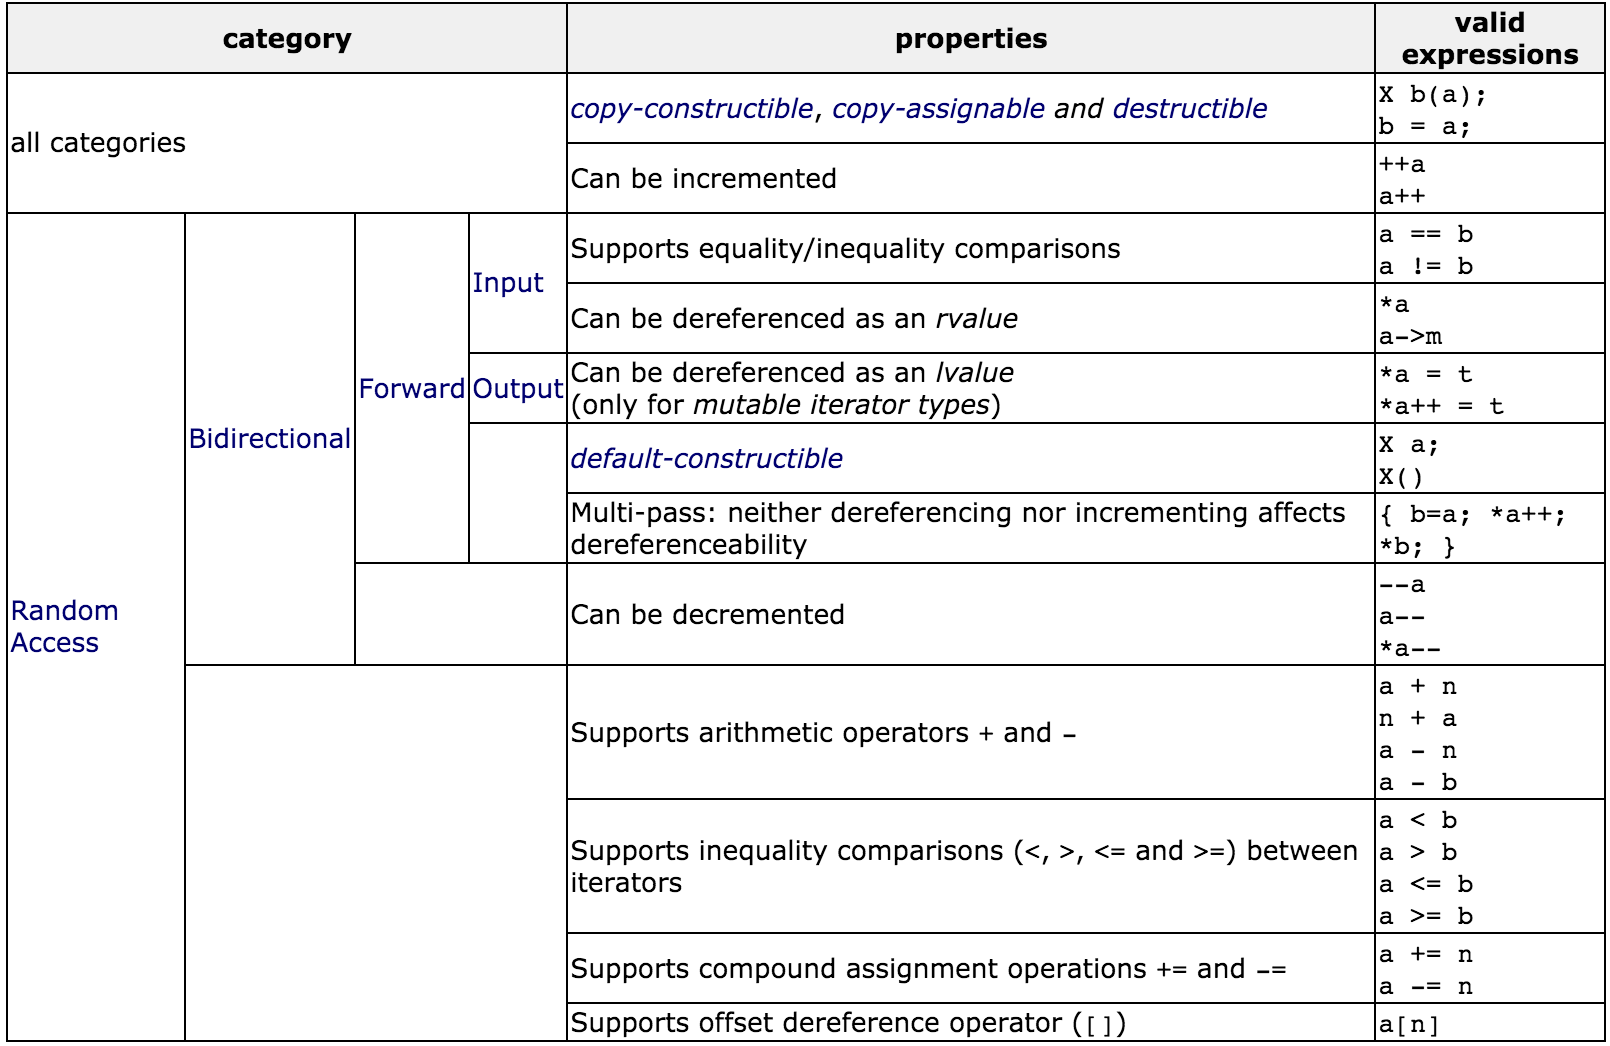
\includegraphics[scale=0.48]{pics/iterator.png}
\end{center}


\item What kind of iterator can be used in specific container and algorithm?
\begin{center}
	  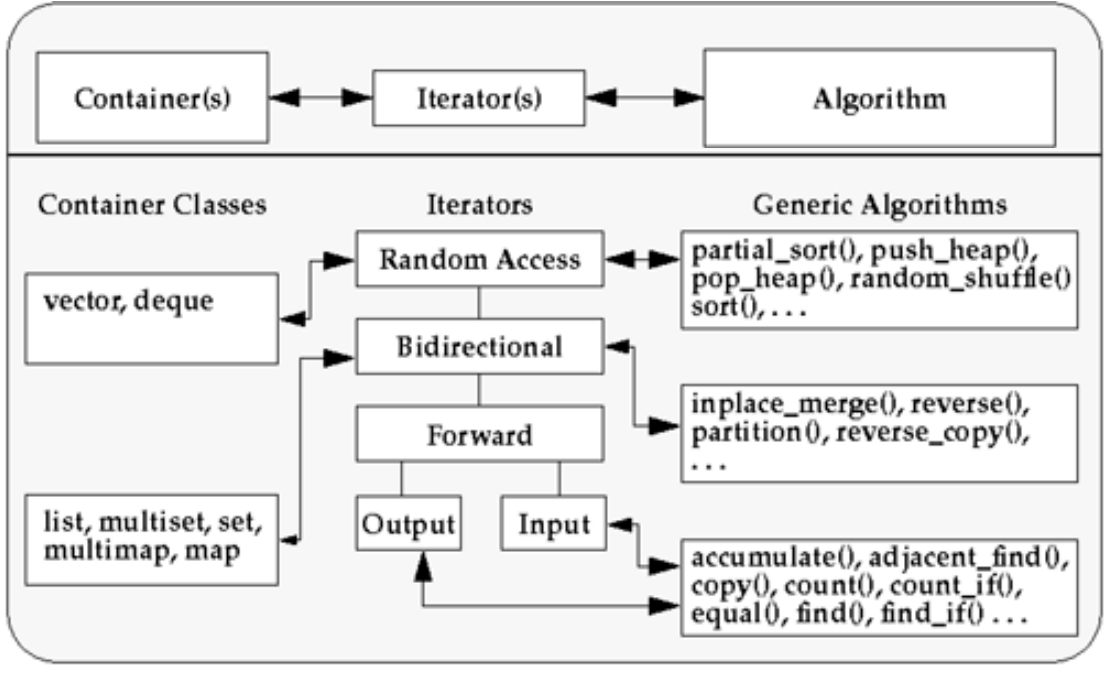
\includegraphics[scale=0.56]{pics/container_it.png}
\end{center}

\item In each container, iterator of container is implemented by itself. In fact, In vector, Maybe iterator is defined by:
\begin{lstlisting}[frame=single, language=c++]
template<type T>
vector{
	....
	typedef T* iterator;
};

vector<int>::iterator ip; //use it outside.
// ++ and -- is done by pointer automatically.
\end{lstlisting}

and All the member function of \texttt{vector} know the iterator very well, inside, it will use T* directly, You can see there is no iterator when you implement container implementation.
\begin{lstlisting}[frame=single, language=c++]
push_back(T x){
*end++ = x;
}  
\end{lstlisting}

	\item When you see the algorithm,  you will see the algorithm is based on template, not inheritance. (You don't need to make type can be cast or not. ). \textbf{Algorithm don't care what iterator really is, It just make sure each iterator can support what operation. }
\begin{lstlisting}[frame=single, language=c++]
template <class InputIterator, class OutputIterator>
  OutputIterator copy (InputIterator first, InputIterator last,
            OutputIterator result);
\end{lstlisting}


\item Common four iterator errors.
\begin{description}



	\item [Valid values:] Is the iterator dereferenceable? For example, writing "\texttt{*e.end()}" is always a programming error, because \texttt{e.end()} is nullptr.

	\item [Valid lifetimes:] Is the iterator still valid when it's being used? Or has it been invalidated by some operation since we obtained it?

	\item [Valid ranges:] Is a pair of iterators a valid range? Is first really before (or equal to) last? Do both really point into the same container?

	\item [Illegal builtin manipulation:] For example, is the code trying to modify a temporary of builtin type, as in "\texttt{--e.end()}" above? (Fortunately, the compiler can often catch this kind of mistake for you, and for iterators of class type, the library author will often choose to allow this sort of thing for syntactic convenience.)

\end{description}


	\item You can inherit your own iterator from \texttt{std::iterator}: yes, that's what it's for.If you mean anything else: no, because none of the STL iterators have virtual destructors. They're not meant for inheritance and a class inheriting from them might not clean up properly. A Good example can be seen link: \\ http://www.cplusplus.com/reference/iterator/iterator/

	\item Two common iterator operation:  \texttt{advance()} and \texttt{distance()}.
\begin{lstlisting}[frame=single, language=c++]
std::list<int>::iterator first = mylist.begin();
std::list<int>::iterator last = mylist.end();

std::advance(first, 3) //
std::cout  << std::distance(first,last)
\end{lstlisting}


	\item That is an example about istream and ostream iterator. \textbf{In this way, you can just think about iostream as a container}.
\begin{lstlisting}[frame=single, language=c++]
vector<Date> e;
copy( istream_iterator<Date>( cin ), 
	istream_iterator<Date>(), back_inserter( e ));

vector<Date>::iterator first = 
	find( e.begin(), e.end(), "01/01/95" );

vector<Date>::iterator last = 
	find( e.begin(), e.end(), "12/31/95" );
*last = "12/30/95";
copy( first, last, ostream_iterator<Date>( cout, "\n" ) );
e.insert( --e.end(), TodaysDate() );
\end{lstlisting}


	\item Another example about \texttt{istreambuf\_iterator}. It supports character-by-character input. Detail can be found in effective STL item 29.
\begin{lstlisting}[frame=single, language=c++, basicstyle=\scriptsize]
std::ostream_iterator<int> out_it (std::cout,", ");
std::copy ( myvector.begin(), myvector.end(), out_it );

ifstream inputFile("aa.txt");
string fileData((istreambuf_iterator<char>(inputFile)), istreambuf_iterator<char>());

ifstream inputFile("aa.dat");
list<int> data((istreambuf_iterator<char>(inputFile)), istreambuf_iterator<char>());
\end{lstlisting}
\begin{description}
	\item[Line 5:] It will just read all the character.(including white character) I don't need format data,
	\item[Line 8:] It wil  read format data, and use white space as delimiter.
\end{description}

	\item IOstreams use streambufs to as their source/target of input/output. Effectively, the streambuf-family does all the work regarding IO and the IOstream-family is only used for formatting and to-string/from-string transformation. Now, \texttt{istream\_iterator} takes a template argument that says what the unformatted string-sequence from the streambuf should be formatted as, like \texttt{istream\_iterator<int>} will interpret (whitespace-delimited) all incoming text as ints. On the other hand, \texttt{istreambuf\_iterator} only cares about the raw characters and iterates directly over the associated streambuf of the istream that it gets passed. Generally, if you're only interested in the raw characters, use an \texttt{istreambuf\_iterator}. If you're interested in the formatted input, use an \texttt{istream\_iterator}.

\end{itemize}

\subsection{Insert iterator}
\begin{itemize}
\item Three common iterator generator: \texttt{inserter(), back\_inserter(), front\_inserter()};  They will produces three insert\_iterator:
\begin{enumerate}
	\item \texttt{insert\_iterator}
	\item \texttt{back\_insert\_iterator}
	\item \texttt{front\_insert\_iterator}
\end{enumerate}

	\item When you use \texttt{insert\_iterator} in an assignment, \texttt{insert\_iterator} will call \texttt{insert()} function.  \newline 
\texttt{back\_insert\_iterator} will call \texttt{push\_back()} and \texttt{front\_insert\_iterator} will call \texttt{push\_front()}. \texttt{insert\_iterator++} has no any operator inside.

	\item  \texttt{std::inserter} is commonly used with sets.

	\item Why do we need these insert iterator? In some algorithm, such as copy and generator, if you read sth from a container, you can use regular iterator, but when you want to write into a container.  You must keep regular iterator is valid. so a method is to use reserve before you write to a container.


	\item Another way is to use \texttt{back\_insert\_iterator}.
\begin{lstlisting}[frame=single, language=c++]
std::vector<int> foo;
for (int i=1; i<=5; i++){ 
	foo.push_back(i); bar.push_back(i*10); 
}
std::copy (bar.begin(),bar.end(),back_inserter(foo));

std::deque<int> foo;
for (int i=1; i<=5; i++){ 
	foo.push_back(i); bar.push_back(i*10); 
}
std::copy (bar.begin(),bar.end(),front_inserter(foo));
\end{lstlisting}

\item Of course, you can use the random access iterators (or any output iterator) in algorithms like \texttt{std::copy}, as third argument, but that assumes the iterator is referencing to existing range — \texttt{*it} and \texttt{++it} are well-defined for the value you passed. You pass them to overwrite the existing elements of the range, whereas \texttt{std::back\_insert\_iterator} adds new elements to the container.

\item For copy algorithm, pass vect.end() is not meaningful, because It's not a valid iterator to support \texttt{*it = new\_obj}.

\end{itemize}


\subsection{Reverse iterator}
\begin{itemize}
\item You need a front-to-back traversal or a back-to-front traversal. The reason for reverse iterators is that the standard algorithms do not know how to iterate over a collection backwards. For example:
\begin{lstlisting}[frame=single, language=c++]
std::find(foo.begin(), foo.end(), L'a');

std::find(foo.rbegin(), foo.rend(), L'a').base()-1;

std::find(foo.end(), foo.begin(), L'a'); //WRONG!! (Buffer overrun)
\end{lstlisting}
\begin{description}
	\item[Line 1:] Returns an iterator pointing to the first 'a'.
	\item[Line 3:] Returns an iterator pointing to the last 'a'.
\end{description}
\item \texttt{reverse\_iterator} can use \texttt{base()} to change a normal iterator, because all the contain member function just receive normal iterator. such as insert and erase.
why \texttt{ri.base()} and ri will have step 1 advance. detail can be seen effective stl item 28.
\begin{lstlisting}[frame=single, language=c++]
reverse_iterator ri =
    find(foo.rbegin(), foo.rend(), L'a');
foo.insert(ri.base()); 
                          
foo.erase((++ri).base()); 
      ri
1 2 3 4 5
        i = ri.base()
\end{lstlisting}
\begin{description}
	\item[Line 3:] you can use \texttt{ri.base()} directly. when you want to insert.
	\item[Line 5:] you can't use \texttt{ri.base()} directly. when you erase what you want. Why? insert happen before the iterator, erase happens on the current iterator. 
\end{description}

\begin{figure}
	\centering
	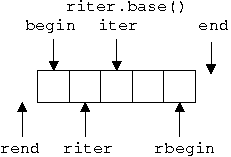
\includegraphics[width=0.3\linewidth]{pics/ri.png}
	\caption{reverse\_iterator }
	\label{fig:ri}
\end{figure}


\end{itemize}

\section{Algorithms}

\subsection{Basic}

\begin{itemize}

\item Effective STL item 43, \textbf{Prefer algorithm calls to hand-written loops}.
\begin{enumerate}
\item  Handing writing is prone to bug.

\begin{lstlisting}
int data[3] ={1,2, 3}
int max = 3;
vector<int> d;
auto current = d.begin();
for( size_t i = 0; i < max; ++i )
	d.insert( current++, data[i] + 41 ); 
\end{lstlisting}
\begin{description}
	\item[Line 6:] Do you see the bug? That is error, because insert will invalid the iterator.
\end{description}

\item You can fix it but with careful design.
\begin{lstlisting}
for( size_t i = 0; i < max; ++i ) {
	current = d.insert( current, data[i] + 41 ); 
	++current;    
}
\end{lstlisting}
\begin{description}
	\item[Line 2 and 3:] Be careful to keep current valid, then increment it when it's safe
\end{description}

\item But a better way is below:
\begin{lstlisting}[numbers=none]
transform( data, data + max, inserter(d, d.begin()) )
\end{lstlisting}
\begin{description}
	\item[Source code:] copy elements from \texttt{data} to the front of \texttt{d}.
\end{description}

\item With a complex algorithm, just use STL algorithm+lambda. 
\begin{lstlisting}[numbers=none]
for( vector<int>::iterator i = v.begin(); i != v.end(); ++i )
if( *i > x && *i < y ) break;

// This is better version now.
vector<int>::iterator i = find_if( v.begin(), v.end(),
                              [x, y](int &i){i>x && i<y} );
\end{lstlisting}

\end{enumerate}
	\item If you need a loop that does something fairly simpler, but would require a confusing tangle of binders and adapters, just use loop.
\begin{lstlisting}[numbers=none]
list<Widget> lw;
type list<Widget>::iterator WI;
for_each(lw.begin(),lw.end(),
                mem_fun_ref(&Widget::redraw) );

transform(data, data+10, inserter(deque, deque.begin()),
        bind2nd(plus<double>(), 41));
\end{lstlisting}

	\item There are four groups: non modifying sequence , mutating sequence, sorting, generalized numeric operations. Detail can be see c++ primer p1286.

	\item Note which algorithm expect sorted ranges:
\begin{lstlisting}[numbers=none]
binary_search, lower_bound, upper_bound, equal_range
set_union, set_intersection, set_difference,
merge, inplace_merge, includes,
unique, unique_copy
\end{lstlisting}



	\item Make sure destination ranges are big enough, see effective STL item 30.
\begin{lstlisting}[frame=single, language=c++]
vector<int> values, result;
int doSth(int x); // function
// make destination range big enough
result.reserve(result.size()+values.size() );

transform(values.begin(), values,end(), result.end(),doSth );

transform(values.begin(), values,end(), back_inserter(result), doSth)  

transform(values.rbegin(), values,rend(), front_insert(result), doSth)
\end{lstlisting}
\begin{description}
	\item[Line 6:] It's error. transform writes its result by making assignment. \texttt{result.end()} has no object at all.
	\item[Line 10:]  result must be a list, use rbegin make insert in front right order
\end{description}

\item Know you sorting options: It makes no sense to sort elements in standard associative containers, because such containers use their comparison functions to remain sorted all the time.

\item For other sequence container, sorting options is below: (1-3) need random iterator. 4 only need bidirection iterator.(list)
  \begin{enumerate}
  \item full sort on vector, string, deque, or array.  use sort or \texttt{stable\_sort}
  \item put only the top n elements in order, \texttt{partial\_sort}
  \item Identify the elements at position n , you need \texttt{nth\_element}
  \item separate the elements of a standard sequence container, do satisfy some criterion, you use partition or \texttt{stable\_partition.}
  \item for list, you should use \texttt{list.sort()} in place of common sort.
  \end{enumerate}
\begin{lstlisting}[numbers=none]
vector<Foo> vf;
bool compare(const Foo& f1, constFoo& f2);
partial_sort(vf.begin(),vf.begin()+20, vf.end(),  compare);
sort(vf.begin(),vf.end(), compare);
nth_element(vf.begin(),vf.begin()+20,vf.end(), compare);

bool good(const Foo &f1)
partition(vf.begin(), vf.end(), good);
\end{lstlisting}

\item Be wary of remove-like algorithm on container of pointers. Delete pointer and free memory which pointer ponits are two different things. That is why we should use \texttt{qunique\_ptr}.
\begin{lstlisting}[numbers=none]
void delAndNULL(Foo*& pf){ // use pointer reference here.
if(!pf->isCertified(){ delete pf; pf = nullptr}
}
for_each(v.begin(),v.end(), delAndNULL);
v.erase(remove(v.begin(),v.end(),
                 static_cast<Foo *>(0) ), v.end());
\end{lstlisting}

\item \textbf{For a algorithms, you need to know three points:}
\begin{enumerate}
	\item What's function  for?
	\item What iterator does it accept? 
	\item What does functor it accept?
	\item What does functor return?
\end{enumerate}
	
\end{itemize}


\subsection{basic notation}

Iterator:  \\
\begin{tabular}{| p{0.2\textwidth} |p{0.75\textwidth}|}
\tophline b, f &	a bidirectional, forward iterator \\
\tophline i,o,a 	&an input, output, random iterator  \\
\tophline(?, ?)	&a pair of iterators as a return value, as in (f,f) \bottomhline
\end{tabular}

functor:  \\
\begin{tabular}{| p{0.2\textwidth} |p{0.75\textwidth}|}
\tophline upred, bpred	& a unary or binary predicate (boolean function or function object)
(generally used to test a single value from a container) \\

\tophline ufunc, bfunc	&  a unary or binary  (value-returning) function or functor \\
\tophline pfunc	& a "parameterless" (value-returning) function (or function object)
(often used to "generate" a value of some kind) \\
\tophline uproc, bproc	& a unary or binary  procedure (void function or function object) \\
\tophline pproc	&  a "parameterless" procedure (void function or functor) \bottomhline
\end{tabular}

Parameter:  \\
\begin{tabular}{| p{0.2\textwidth} |p{0.75\textwidth}|}
\tophline n, v, \&  & 	a quantity (or size). A value. reference to a value \bottomhline
\end{tabular}

\subsection{Nonmutating algorithms}
There are five big group inside this Nonmutating group, you can remember as CCMFS (cc make friends) They are \textbf{count, compare, max, find and search}.


\subsubsection{count}
\begin{tabular}{| p{0.25\textwidth} |p{0.4\textwidth}|p{0.2\textwidth}|}
\tophline n count(i,i,\& ) & Count the items in a range that match a value and return that count.& \multirow{2}{*}{ \parbox{0.2\textwidth}{count will not stop when it find match. } }    \\
\ifdefined\pdfbook  \cline{1-2} \fi n count\_if(i,i,upred)  & Count the items in a range that satisfy a predicate and return that count. & \bottomhline
\end{tabular}

\subsubsection{find}

\textbf{2: linear time Searching} \\
\begin{tabular}{| p{0.3\textwidth} |p{0.65\textwidth}|}
\tophline \specialcell[t]{f adjacent\_find(f,f) \\
f adjacent\_find(f,f, bpred)
   }&  the first pair of equal adjacent values in a range and return an iterator pointing to the first value of the pair.  \\

\tophline i find(i,i,\&)  &
return an iterator pointing to the value or end  \\

\tophline i find\_if(i,i,upred)  &
satisfies a predicate and return an iterator pointing to the first such value, or to the end  \bottomhline
\end{tabular}


\textbf{3: Search for a single element from a range} \\
\begin{tabular}{| p{0.4\textwidth} |p{0.55\textwidth}|}

\tophline \specialcell[t]{ f1 find\_first\_of(f1,f1,f2,f2) \\
f1 find\_first\_of(f1,f1,f2,f2,bpred) } & std::find\_first\_of searches for a single element from a range within another range.
\bottomhline
\end{tabular}


\subsubsection{Searching}

\textbf{1:Sorted range Searching}  \\
\begin{tabular}{| p{0.35\textwidth} |p{0.6\textwidth}|}

\tophline bool binary\_search(f,f,\&)&  sorted range of values and return bool.
\bottomhline
\end{tabular}


\textbf{4: Below 3 algorithms search for a whole range of elements within another range }\\
\begin{tabular}{| p{0.35\textwidth} |p{0.6\textwidth}|}
\tophline \specialcell[t]{f1 search(f1,f1,f2,f2) \\
f1 search(f1,f1,f2,f2) } &
first occurrence of a second range of values within a first range . return an iterator pointing to the first value of that first match. or end of the first range  \\

\tophline \specialcell[t]{ f1 find\_end(f1,f1,f2,f2) \\
f1 find\_end(f1,f1,f2,f2,bpred) } &
the last occurrence of a second range of values in a first range of values and return an iterator pointing to the first value of that last match within the first range, or pointing to the end of the first range(not find) \\

\tophline  \specialcell[t]{f search\_n(f,f,n,\&) \\
f search\_n(f,f,n,\&,bpred) }  &
For a contiguous sequence of n values each equal to \&, return iterator to the first of those values, or  the end of the range \bottomhline
\end{tabular}


\subsubsection{Comparing}
\begin{tabular}{| p{0.55\textwidth} |p{0.4\textwidth}|}
\tophline \specialcell[t]{bool equal(i1,i1last, i2) \\
bool equal(i1,i1last,i2,bpred) } &  Check if the values in two ranges match. \\

\tophline
\specialcell[t]{bool lexicographical\_compare (i1,i1last,i2,i2last) \\
bool lexicographical\_compare (i1,i1last,i2,i2last,bpred) }  & Compare two ranges lexicographically, and return true if the first range is less than the second; otherwise return false. \\

\tophline
 \specialcell[t]{ (i1,i2) mismatch(i1,i1last,i2) \\ (i1,i2) mismatch(i1,i1last,i2, bpred) }
 & Search two ranges for the first two items in corresponding positions that don't match, and return a pair of iterators pointing to those two items.
 
\bottomhline
\end{tabular}
\begin{itemize}
\item An example to use \texttt{equal}:
\begin{lstlisting}[numbers=none]
bool is_palindrome(const std::string& s){
    return std::equal(s.begin(), s.begin() + s.size()/2, s.rbegin());
}
\end{lstlisting}
\end{itemize}

\subsubsection{Max and Min}
\textbf{Min/Max} \\
\begin{tabular}{| p{0.3\textwidth} |p{0.6\textwidth}|}
\tophline \specialcell[t]{\& min(\&,\&)  \\
\& min(\&,\&,bpred)   }&  Find the minimum of two values and return a reference to that value.
\\

\tophline  \specialcell[t]{
\& max(\&,\&) \\
\& max(\&,\&,bpred)     } & Find the maximum of two values and return a reference to that value.    \\

\tophline \specialcell[t]{
f min\_element(f,f)  \\
f min\_element(f,f,bpred)  } & Find the minimum value in a range and return an iterator pointing to that value.   \\

\tophline  \specialcell[t]{
f max\_element(f,f)  \\
f max\_element(f,f,bpred)   } & Find the maximum value in a range and return an iterator pointing to that value.   \bottomhline
\end{tabular}

\subsection{Mutating algorithms}
\begin{itemize}
	\item In this group, remember RRRPPCFSM(RRRPP copy friends many time). They are \textbf{replace, remove, random, partition, permuting, copy, filling, swapping and math}. 
\end{itemize}

\subsubsection{for\_each}
\begin{tabular}{| p{0.3\textwidth} |p{0.43\textwidth}|p{0.18\textwidth}|}
	\tophline ufunc for\_each(i,i,ufunc) &Apply a function to every item in a range and return the function. &  ufunc may not return value. 
	\bottomhline
\end{tabular}
\newline 

\begin{lstlisting}[numbers=none]
void fun(int n){
	cout<<" "<<n;
} //all function definition end no semicolon

struct Sum{
	Sum(): sumEven{0} { }  //no semicolon here
	void operator()(int n) {if(n%2 ==0) ; sumEven += n;}
		int sumEven;
	}; // type definition need semicolon
	
	vector<int> nums{3, 4, 2, 8, 15, 267};
	for_each(nums.begin(), nums.end(), fun);
	Sum s = for_each(nums.begin(), nums.end(), Sum());
	for_each(nums.begin(), nums.end(), [sumEven](int n){
		if(n%2==0) sumEven+=n;
	});
\end{lstlisting}
	
	\begin{itemize}
		\item \texttt{for\_each} need a functor, So when to use \texttt{for\_each} equals another question, when use functor.
		\begin{enumerate}
			\item For fun example, a better way is \texttt{for(auto e: nums)\{cout<<e<<" ";\}}. Here just demonstrate that  you can input fun.
			
			\item For struct Sum just use once, lambda function is better, because it is cleaner.
			
			\item If functor need to be 1)customized state and 2)reuse many time, then functor is better.
\begin{lstlisting}[numbers=none]
struct GreatThanX{
	GreatThanX(int x): cutoff{x} { } 
	bool operator()(int n) { if(n>x) ; 
		return true; return false; }
	int cutoff;
};

vector<int> nums{3, 4, 2, 8, 15, 267};
find_if(nums.begin(), nums.end(),GreatThanX(3));
copy_if(nums.begin(), nums.end(),GreatThanX(7));
..........
\end{lstlisting}
			\item \textbf{Only functor can be use a argument input to map or set container set}. See below examples.
			
\begin{lstlisting}[numbers=none]
struct lex_compare {
	bool operator() (const int64_t& lhs, const int64_t& rhs) const{
		stringstream s1,s2;        s1 << lhs;  s2 << rhs;
		return s1.str() < s2.str();
	}
};
set<int64_t, lex_compare> s;
\end{lstlisting}
			
			\item Lambdas aren't useful for more complex scenarios because they weren't made for them. They provide a short and concise way of creating simple function objects for correspondingly simple situations.
			
			\item You also can use bind on a name lambda. if lambda is easy, just rewrite it. 
\begin{lstlisting}[numbers=none]
auto f = [](int x, int y){if(y>x) return true; return false;} ;
auto f1 = bind(f, 3, placeholders::_1) // GreatThanX(3);
if(f1(8)) cout<<"8>3"<<endl;
\end{lstlisting}			
		\end{enumerate}
		
	\end{itemize}

	\textbf{Transforming}  \\
	\begin{tabular}{| p{0.35\textwidth} |p{0.3\textwidth}|p{0.25\textwidth}|}
		\tophline \specialcell[t]{ o transform(i1,i1end,o,ufunc) \\o transform(i1,i1end,i2, o, bfunc) }
		&Transform one range of values into another.
		& Ret of ufunc or bfunc writed to o. 
		
		\bottomhline
	\end{tabular}
	
	\begin{itemize}
		\item If output is associate container, you need use \texttt{inserter( )} function to get inserter iterator.
		\begin{lstlisting}[frame=single, language=c++, mathescape=true]
			std::transform(a.begin(), a.end(),
			std::inserter(set, set.begin()), modify);
			
			std::transform(a.begin(), a.end(), b.begin(),
			a.begin(), plus<int>() );
		\end{lstlisting}
		\begin{description}
			\item[Source code:] 1) you can make in place modification. 2) plus minus, multiplies, divides, modulus, negate, equal\_to are often used in transform algorithms.
		\end{description}
		
	\end{itemize}


\subsubsection{swapping}
\begin{tabular}{| p{0.35\textwidth} |p{0.6\textwidth}|}
\tophline iter\_swap(f,f) &
Swap the values pointed to by the two iterators.  \\
\tophline swap(\&,\&) &
Swap the two values.  \\
\tophline f2 swap\_ranges(f1,f1end,f2) &
Swap two ranges of values and return an iterator pointing to the end of the second range.  \bottomhline
\end{tabular}



\subsubsection{copy}

\begin{tabular}{| p{0.35\textwidth} |p{0.6\textwidth}|}
\tophline o copy(i,i,o) & Copy a range of items to a destination and return an iterator pointing to the end of the copied range.   \\
\tophline b2 copy\_backward(b1,b1last, b2)  & Copy a range of items backwards to a destination and return an iterator pointing to the end of the copied range.    \bottomhline
\end{tabular}



\begin{lstlisting}[frame=single, language=c++]
for (int i=1; i<=5; i++)
    myvector.push_back(i*10);

copy(myvector.begin(), myvector.end(),
	 myvector.begin()+3)

myvector.resize(myvector.size()+3)
copy_backward(myvector.begin(), myvector.begin()+5, 
	myvector.end())
\end{lstlisting}
\begin{description}
	\item[Line 4:] error, when source and targe is overlap, you have to use backward copy
	\item[Line 7:]pay attention, \texttt{copy\_backward}, *(--last) = if you want copy to position 3, you need to input position 4. or you can input \texttt{vector.end()} as target, but for copy, you can't input \texttt{vector.end()}. First, resize, then use\texttt{ myvector.end()} as the last parameter.

\end{description} 

\subsubsection{Filling and Generating}
\textbf{Filling} \\
\begin{tabular}{| p{0.3\textwidth} |p{0.6\textwidth}|}
\tophline fill(f,f,\& ) & Set every item in a range to a particular value.  \\
\tophline fill\_n(o,n,\& )  & Set n items to a particular value.   \bottomhline
\end{tabular} \\


\textbf{Generating} \\

\begin{tabular}{| p{0.3\textwidth} |p{0.6\textwidth}|}
\tophline generate(f,f,pfunc)  & Fill a range with generated values.   \\
\tophline generate\_n(o,n,pfunc)  & Generate a specified number of values.   \bottomhline
\end{tabular}

\begin{lstlisting}[numbers=none]
std::vector<int> v(5);
std::generate(v.begin(), v.end(), std::rand); // Using the C function rand()

int n = {0};
std::generate(v.begin(), v.end(), [&n]{ return n++; });
\end{lstlisting}

\subsubsection{Math}
\begin{tabular}{| p{0.45\textwidth} |p{0.5\textwidth}|}
\tophline \specialcell[t]{v accumulate(i,i,v) \\
v accumulate(i,i,v,bfunc)  }&  Add an initial value and the values in a range, return sum.
\\

\tophline \specialcell[t]{
o adjacent\_difference (i,i,o) \\
o adjacent\_difference \\ (i,i, o, bfunc)   } & Calculate the difference between adjacent pairs of values, write the differences to an o, and return the end of that output range.    \\

\tophline
\specialcell[t]{ v inner\_product (i1,i1last,i2,vInitial) \\
v inner\_product (i1,i1last,i2,v,bfunc1,bfunc2)}  & Calculate the inner product of two ranges and return that value plus vInitial.  \\

\tophline  \specialcell[t]{
o partial\_sum(i,i,o)  \\
o partial\_sum(i,i,o, bfunc)   } & Fill a range with running totals and return an iterator pointing to.   \bottomhline
\end{tabular} \\
\begin{itemize}

\item An example about \texttt{partial\_sum}.

\begin{lstlisting}[numbers=none]
std::vector<int>v(10, 2); // new initialize method
std::partial_sum(v.begin(), v.end(),
          std::ostream_iterator<int>(std::cout, " "));
    //2 4 6 8 10 12

std::partial_sum(v.begin(), v.end(), v.begin(),
                            std::multiplies<int>());
std::cout << "The first 10 powers of 2 are: ";
 for (auto n : v) {
      //2 4 8 16 32
    }
\end{lstlisting}
\item An example about \texttt{accumulate}.

\begin{lstlisting}[numbers=none]
std::vector<int> v{1, 2, 3, 4, 5, 6, 7, 8, 9, 10};
int sum = std::accumulate(v.begin(), v.end(), 0);
int product = std::accumulate(v.begin(), v.end(), 1, multiplies<int>());

string s=accumulate(v.begin(), v.end(),std::string{},
    [](const std::string& a, int b) {
    	return a.empty() ? to_string(b): a + '-' + to_string(b); 
    });
\end{lstlisting}

\item An example about \texttt{adjacency\_difference}. produces fibonacci.
\begin{lstlisting}[numbers=none]
v = {1, 1, 1, 1, 1, 1, 1, 1, 1, 1};
std::adjacent_difference(v.begin(), v.end() - 1, v.begin() + 1, std::plus<int>());
\end{lstlisting}

\item Difference some algorithms
\begin{enumerate}
\item For \texttt{accumulate}, input a init, -->calculate(init, element)-->return it to init.
\item For \texttt{adjacent\_difference}:   first -> dfirst,  f(first+1, first)-->dfirst+1; Pay attention, for first element, assign it directly.
\item For \texttt{partial\_sum} function, you can think it as accumulate, \textbf{accumulate just return one value, but \texttt{partial\_sum} return many value, and write them back to target iterators one by one.  }
\item \texttt{accumulate} and \texttt{inner\_product} return one value, \texttt{partial\_sum} and \texttt{adjacent\_difference} return a list of value.
\end{enumerate}

\end{itemize}



\subsubsection{Partitioning}
\begin{tabular}{| p{0.35\textwidth} |p{0.6\textwidth}|}
\tophline \specialcell[t]{nth\_element(r,r,r) \\
nth\_element(r,r,r,bpred)   }&  Partition a range of values so that the value pointed to by the middle r in the parameter list is in its correct sorted position, and no element to its left is greater than any element to its right. \\

\tophline  \specialcell[t]{
b partition(b,b,upred)    } & Partition a range of values using a predicate, and return an iterator pointing to the first value for which upred returns false.   \\

\tophline  \specialcell[t]{
b stable\_partition(b,b,upred)     } & Partition a range using a predicate without altering the relative order of the values, and return an iterator pointing to the first value for which upred returns false.  \bottomhline
\end{tabular}


\begin{itemize}
\item  An example of \texttt{partition}:
\begin{lstlisting}[numbers=none]
std::vector<int> v = {0,1,2,3,4,5,6,7,8,9};
auto it = std::partition(v.begin(), v.end(), [](int i){return i % 2 == 0;});
                     
std::copy(std::begin(v), it, std::ostream_iterator<int>(std::cout, " "));
         
std::copy(it, std::end(v), std::ostream_iterator<int>(std::cout, " "));
\\output: 0 8 2 6 4   5 3 7 1 9
\end{lstlisting}

\item \textbf{Partition return: Iterator to the first element of the second group.}

\item Gather all eligible element around iterator p
\begin{lstlisting}[numbers=none]
template <typename BiIt, typename UnPred> 
auto gather(BiIt f, BiIt l, BiIt p, UnPred s) -> std::pair <BiIt, BiIt>{
	return { stable_partition(f, p, not1(s)), 
		stable_partition(p, l, s) };
}	
\end{lstlisting}


\item All of the elements before this new nth element are less than or equal to the elements after the new nth element. Who are my top 20 salespeople?" For example, nth\_element( s.begin(),
s.begin()+19, s.end(), SalesRating ); puts the 20 best elements at
the front.
\item If you use nth\_element on most of the range, It may be slower than a full sort.
\end{itemize}




\subsubsection{Permuting}

\begin{tabular}{| p{0.35\textwidth} |p{0.6\textwidth}|}
\tophline \specialcell[t]{bool next\_permutation(b,b) \\
bool next\_permutation\\ (b,b,bpred)    }&  Change a range of values to the next lexicographic permutation of those values, and return true, or false if no next permutation exists.
 \\

\tophline  \specialcell[t]{
bool prev\_permutation (b,b)  \\
bool prev\_permutation \\ (b,b, bpred)     } & Change a range of values to the previous lexicographic permutation of those values, and return true, or return false if no previous permutation exists.  \bottomhline
\end{tabular}

\begin{lstlisting}[numbers=none]
int a[] = {1,2,3};
do {
    cout << a[0] << ' ' << a[1] << ' ' << a[2] << '\n';
} while ( std::next_permutation(a,a+3) );
1 2 3 // 1 3 2 //2 1 3
2 3 1 //3 1 2  //3 2 1
\end{lstlisting}


\begin{tabular}{| p{0.35\textwidth} |p{0.6\textwidth}|}
\tophline rotate(f,f,f)  & Rotate a range of values by n positions.  \\
\tophline rotate\_copy(f,f,f,o) &   Copy and rotating it by n position.  
\bottomhline
\end{tabular}


\begin{itemize}

\item Rotates the order of the elements in the range [first,last), in such a way that the element pointed by middle becomes the new first element.


\begin{lstlisting}[numbers=none]
for (int i=1; i<10; ++i) myvector.push_back(i);
// 1 2 3 4 5 6 7 8 9
rotate(myvector.begin(), myvector.begin()+3,myvector.end());
// 4 5 6 7 8 9 1 2 3
\end{lstlisting}

\item you can use rotate in insert sort method. also use in slide. Detail can be found in "Top 5 Beautiful C++ std Algorithms Examples"

\begin{lstlisting}[breaklines, basicstyle=\scriptsize]
for (auto i = start; i != end; ++i)
std::rotate(std::upper_bound(start, i, *i), i, std::next(i));

template <typename It> 
auto slide(It f, It l, randIter p) -> std::pair<It, It>{
	if (p < f) return { p, std::rotate(p, f, l) };
	if (l < p) return { std::rotate(f, l, p), p };
	return { f, l };
}	
\end{lstlisting}
\begin{description}
	\item[line 2:] rotate(a, b, c) is [a,b) and [b,c) scope. they are all left close, right open scope. In this way, you can understand why we need \texttt{std::next(i)} here.
	\item[line 6-7:] when p <f, p is the first element position, when p>l, p is the last element position. That will help you to understand slide algorithm. 
\end{description}

\end{itemize}

\begin{tabular}{| p{0.3\textwidth} |p{0.6\textwidth}|}
\tophline reverse(b,b) &  Reverse the order of all values in a range of values. \\
\tophline reverse\_copy(b,b,o) &  Reverse and copy  \\ \tophline
\end{tabular}



\subsubsection{Random/shuffing}
\begin{tabular}{| p{0.35\textwidth} |p{0.6\textwidth}|}
\tophline \specialcell[t]{random\_shuffle(r,r)  \\
random\_shuffle(r,r,ranGen)    }&  Randomize a range of values, and use the random generator function ranGen, if supplied, rather than an internal random generator. \bottomhline
\end{tabular}


\subsubsection{Removing}
\begin{tabular}{| p{0.35\textwidth} |p{0.6\textwidth}|}
\tophline \specialcell[t]{remove(f,f,\&)  \\
remove\_if(f,f,upred)    } &  Remove from a range of values all values that match a give value or satisfy a predicate \\

\tophline \specialcell[t]{ remove\_copy(i,i,o,\&) \\
remove\_copy\_if(i,i,o,upred)}  & Copy a range of values, removing all values that match a given value. \bottomhline

\end{tabular}

\begin{itemize}
\item These algorithms cannot be used with associative containers such as std::set and std::map because ForwardIt does not dereference to a MoveAssignable type (the keys in these containers are not modifiable)
\item \texttt{list} has its own \texttt{remove}.
\item Then, remove only can be used in erase remove idiom in \texttt{vector} and string.
\end{itemize}

\textbf{Filtering , should used on sorted container} \\
\begin{tabular}{| p{0.35\textwidth} |p{0.6\textwidth}|}
\tophline \specialcell[t]{f unique(f,f) \\
f unique(f,f,bpred) }&  Collapse each group of consecutive duplicate values to a single value, and return an iterator pointing to the end of the modified range.
\\

\tophline \specialcell[t]{
o unique\_copy(i,i,o)  \\
o unique\_copy(i,i,o,bpred)  } & Copy a range of values, performing the same action as unique above, and return an iterator pointing to the end of the new range.   \bottomhline

\end{tabular}
\begin{itemize}
	\item unique need to be sort first. 
	\item Just like remove, unique need erase unique idiom.
	\item You can think unique has three steps. sort, unique, erase.
\end{itemize}

\begin{lstlisting}[numbers=none]
std::sort(v.begin(), v.end()); // {1 1 2 3 4 4 5}
last = std::unique(v.begin(), v.end());
v.erase(last, v.end());  // Above shows three steps, 
\end{lstlisting}

\begin{lstlisting}[numbers=none]
int myints[] = {10,20,20,20,30,30,20,20,10};
std::vector<int> myvector (myints,myints+9);

std::vector<int>::iterator it;
it = std::unique (myvector.begin(), myvector.end());
// 10 20 30 20 10 ?  ?  ?  ?
\end{lstlisting}


\subsubsection{Replacing}
\begin{tabular}{| p{0.35\textwidth} |p{0.6\textwidth}|}
\tophline \specialcell[t]{  replace(f,f,\&,\&) \\
 replace\_if(f,f,upred,\&) } &
Replace, within a range of values, one specified value(satisfies a predicate) with another value.  \\

\tophline \specialcell[t]{ replace\_copy(i,i,o,\&,\&)  \\
 replace\_copy\_if(i,i,o,upred,\&)} &
Copy  replacing one specified value with another specified value.  \\
\tophline
\end{tabular}

\subsection{sorting}

\subsubsection{binary search}

\begin{tabular}{| p{0.3\textwidth} |p{0.45\textwidth}|p{0.2\textwidth}|}
\tophline \specialcell[t]{(f,f) equal\_range(f,f,\&) \\
(f,f) equal\_range(f,f,\&,bpred) }& Find the lower bound and upper bound of a value within a range and return a pair of iterators  .
& \multirow{3}{*}{ \parbox{0.2\textwidth}{1)container should be sorted firstly,  2) order by default < or bpred. 3) Sorted by bpred, find by bpred. } } \\

\ifdefined\pdfbook \cline{1-2} \fi  \specialcell[t]{f lower\_bound(f,f,\&) \\
f lower\_bound(f,f,\&,bpred)} & Find the lower bound of a value within a range and return an iterator pointing to it.
 &  \\

\ifdefined\pdfbook  \cline{1-2} \fi \specialcell[t]{f upper\_bound(f,f,\&) \\ f upper\_bound(f,f,\&,bpred) }
& Find the upper bound of a value within a range and return an iterator pointing to it.
&  \bottomhline
\end{tabular}


\subsubsection{set}.
\begin{tabular}{| p{0.45\textwidth} |p{0.5\textwidth}|}
\tophline \specialcell[t]{ bool includes(i1,i1,i2,i2) \\
bool includes(i1,i1,i2,i2,bpred) }  &
Search for \textbf{all values from the second range in the first range} and return true if found, or false  \\
\tophline \specialcell[t]{o set\_difference(i1,i1,i2,i2,o) \\
o set\_difference(i1,i1,i2,i2,o,bpred) } &
in the first range but not in the second range and return the end of that output range. \\

\tophline \specialcell[t]{o set\_intersection(i1,i1,i2,i2,o)  \\
o set\_intersection(i1,i1,i2,i2,o,bpred) } &
 in the first range and also in the second range and return the end of that output range. \\

\tophline \specialcell[t]{o set\_union(i1,i1,i2,i2,o) \\
o set\_union(i1,i1,i2,i2,o,bpred) } &
either in the first range or in the second range and return the end of that output range. \\

\tophline \specialcell[t]{o set\_symmetric\_difference(i1,i1,i2,i2,o)  \\
o set\_symmetric\_difference(i1,i1,i2,i2,o,bpred) } &
 not common to both ranges and return the end of that output range.  \bottomhline

\end{tabular}
\begin{itemize}
\item All algorithm need two ranges should be sorted.

\begin{center}
	\includegraphics[width=0.25\linewidth]{pics/set_diff.png}
	\includegraphics[width=0.25\linewidth]{pics/set_sys_diff.png}
\end{center}

\end{itemize}



\subsubsection{sort}
\begin{tabular}{| p{0.33\textwidth} |p{0.6\textwidth}|}
\tophline \specialcell[t]{partial\_sort(r,r,r) \\
partial\_sort(r,r,r,bpred) } &
Sort all values till first part of range is in sorted order. \\

\tophline \specialcell[t]{r partial\_sort\_copy(i,i,r,r) \\
r partial\_sort\_copy \\ (i,i,r,r,bpred) } &
Partially sort a range of values (as above) and copy \textbf{as many values as will fit into an output range.}\\

\tophline \specialcell[t]{sort(r,r) \\
sort(r,r,bpred) } &
Sort a range of values.\\

\tophline \specialcell[t]{ stable\_sort(r,r) \\
stable\_sort(r,r,bpred) } &
Sort and maintaining the same relative order of duplicate values.\bottomhline
\end{tabular}


\begin{lstlisting}[numbers=none]
sort(begin(vs),end(vs), [](const string& str1, const string& str2){
     return lexicographical_compare(begin(str1), end(str1), begin(str2), end(str2),[](auto ch1, auto ch2){
            return tolower(ch1)<tolower(ch2);
        });
    } );
    
copy(begin(vs),end(vs), ostream_iterator<string>(cout, " "));
    
string str1 = "Abc";
string str2 = "abc";
cout<<equal(begin(str1),end(str1), begin(str2),end(str2), [](auto a, auto b){return tolower(a) ==tolower(b); });
\end{lstlisting}

\subsubsection{Merging}
\begin{tabular}{| p{0.35\textwidth} |p{0.6\textwidth}|}
\tophline \specialcell[t]{inplace\_merge(b,b,b) \\
inplace\_merge(b,b,b,bpred)   }&  Merge two sorted ranges, in place, into a single sorted range.
\\

\tophline  \specialcell[t]{
o merge(i1,i1,i2,i2,o)  \\
o merge(i1,i1,i2,i2,o,bpred)    } & Merge two sorted ranges into a single sorted range.   \\
\tophline
\end{tabular}

\subsubsection{heap}
\textbf{Heap} \\
\begin{tabular}{| p{0.28\textwidth} |p{0.4\textwidth}|p{0.2\textwidth}|}
\tophline \specialcell[t]{make\_heap(r,r)  \\
make\_heap(r,r,bpred) }&  Make a range of values into a heap.
& \multirow{4}{*}{ \parbox{0.2\textwidth}{It nees random iterator. priority\_queue use them inside. You don't use them directly } } \\

\ifdefined\pdfbook  \cline{1-2} \fi  \specialcell[t]{
o pop\_heap(r,r) \\
o pop\_heap(r,r,bpred)   } & Delete the first value from a heap.  &  \\

\ifdefined\pdfbook  \cline{1-2} \fi  \specialcell[t]{
push\_heap(r,r) \\
push\_heap(r,r,bpred)  } & Insert the last value of a range into a heap. &  \\

\ifdefined\pdfbook  \cline{1-2} \fi \specialcell[t]{
sort\_heap(r,r) \\
sort\_heap(r,r,bpred)   } & Sort a heap.  &  \\
\tophline
\end{tabular}

\begin{lstlisting}[frame=single, language=c++, mathescape=true]
vector<int> vi = {2, 4, 1, 3, 5,6,7};
make_heap(begin(vi),end(vi)); // inpace modify

//after you pop_heap, you need to use v.pop_back()
//to make begin(vi), end(vi) is still heap. 
v.pop_heap(begin(vi),end(vi));
v.pop_back();  //pop_back and pop_heap must appear together.

//if you want to use push_heap, you have to call push_back first. 
v.push_back(10);  //push_back and push_heap must appear together
v.push_heap(v.begin(vi) ,end(vi));

sort_heap(v.begin(vi) ,end(vi)); //still inpace modify
\end{lstlisting}



\subsection{Summary}
\subsubsection{Nonmutating Algorithms}
\begin{itemize}
	\item Nonmutating Algorithms(Observer semantic)
	\begin{center}
		\includegraphics[width=1.0\linewidth]{pics/stl1.png}
	\end{center}
	
\end{itemize}

\subsubsection{Mutating Algorithms}
\begin{itemize}
	\item \texttt{remove} just keep good one, \texttt{partition} put good one in front, bad one in back. \texttt{nth\_element} is strong version of partition.
	
	\item \texttt{accumulate} has fold semantic. I introduce a lot in functional chapter. There are more good examples about how to use \texttt{accumulate} there. 
	
	\item \texttt{transform} has map semantic. It is important component in functional programming.
	
	\item Another important semantic in functional programming is \textbf{filter}, you can use \texttt{copy\_if} or \texttt{remove\_if} to implement it.
	
	\begin{center}
		\includegraphics[width=1.0\linewidth]{pics/stl2.png}
	\end{center}
	
	\item All these functions begins with letter R. \texttt{unique} can be thought as a kind of \texttt{remove}.\textbf{ All algorithms don't change container's size, just change it contents.}
	
	\item \texttt{rotate} is also important algorithm. For example, you can use it to implement insert sort easily. 
	
	\begin{center}
	\includegraphics[width=1.0\linewidth]{pics/std3.png}
	\end{center}
	
\end{itemize}
	
\subsubsection{Sorting and search in sorted container}
\begin{itemize}
	\item All search methods in the below figure must applied into sorted container.
	\item \texttt{make\_heap} needs random access iterator.
	
	\begin{center}
	\includegraphics[width=1.0\linewidth]{pics/std4.png}
	\end{center}

\end{itemize}

\section{Function object}
\subsection{Basic knowledge of callable object}

\begin{itemize}
	
	\item  In C language, we use function pointer.
\begin{lstlisting}[numbers=none]
int(*pf)(int, int); //declare a pointer function
int fun1(int i,int j);
pf = fun1  // or pf=&fun1; we usually skip &.
(*pf)(1,2) //or pf(1,2);
\end{lstlisting}

	\item In C++, generic algorithms can also accept function by template argument.
\begin{lstlisting}[]
void fun(int i) {
	//do stuff
}

for_each(a.begin(), a.end(), fun);
\end{lstlisting}
\begin{description}
	\item[Line 5:] \texttt{for\_each} is template function, so we need input variable. Here just input fun name, it's function pointer usage. function pointer is variable, not a type.
\end{description}

\item But passing function pointer has shortcomings:
\begin{enumerate}
	\item Can't be inline.
	\item Sometimes it can't be compile due to different compiler implementation.
	\item You can't adapt or custom it.
\end{enumerate}
So STL invented a functor(function object). It is class or structure objects for which the \texttt{operator ()} is overload.

\begin{lstlisting}
class functor { // also call function objects
public:
  void operator()(int i);
};

for_each(a.begin(), a.end(), functor()); //need value, not type
\end{lstlisting}
\begin{description}
	\item[Line 1:] here, use functor, (class object); overload operator();
	\item[Line 6:] function accept variable, not type. You must use functor() to produce a temporary functor obj.
\end{description}

	\item  You can use struct or class. If you want to have a private customized value, you have to use class to build a functor.  Such as cutoff value in below code.
\begin{lstlisting}[frame=single, language=c++]
struct less_than_7 : std::unary_function<int, bool>{
    bool operator()(int i) const { return i < 7; }
};

class less_than_value : std::unary_function<int, bool>{
    less_than_value(int x) :value(x) {};
    bool operator()(int i) const { return i < value; }
private:
    int value;
};

count_if(v.begin(),v.end(), std::not1(less_than_7()));
count_if(v.begin(),v.end(),std::not1(less_than_value(7)));
\end{lstlisting}
\begin{description}
	\item[Line 1:] you can use class instead struct, but you need to make operator() public, in struct, default is public, so struct is better! Why do we need to inherit from \texttt{unary\_funciton}, in this way, we can use \texttt{std::not1} to adapt it. \textbf{This is old style and not recommend to use in modern C++.}
\end{description}


   \item In previous example, you can see advantage of usage \texttt{less\_than\_value}.
   \begin{enumerate}
   \item You can inherit from  template \texttt{unary\_function} when you declare a functor, then you functor is adaptable by \texttt{std::not1}.

   \item you can change value when you build a \texttt{less\_than\_value} functor.

   \item set or map are template class. So it only accept type, not function, If you want to give set or map a customized compare function,  you have to use functor to define a type.
\begin{lstlisting}[frame=single, language=c++]
class yanCompare{
    bool operator()(string &s1, string &s2){....;}
};

set<string, yanCompare> setDic;
remove_if(...yanComare() );
\end{lstlisting}
\begin{description}
	\item[Line 5:] template container need type. so we have to input type, so we input \texttt{yanCompare,} It's a class type. Just \texttt{yanCompare}, no() follow it. pass into a type, not obj.
	\item[Line 6:] template function is a function, we have to input value, so we pass variable or expression. in previous example,\texttt{ yanCompare()} produce a obj variable. \texttt{yanCompare()} to produce a temporary variable, then to pass it to \texttt{remove\_if}.
\end{description}
 
\end{enumerate}

\item Based on previous example, I would like to say something about \textbf{type, variable, expression, value}.
\begin{enumerate}
	\item type is build-in type, custom type(class, struct), and pointer, reference type.
	\item variable has a name, value and type.
	\item expression has no name but has value and type.
	\item value can be divided by three categories.
	\item Given a variable or expression, we need to know its type, we can use auto, T in template and decltype. detail can be seen "type inference" section.
	
	\item Given a container, we can get \texttt{value\_type} by predefined type information in container.
	
	\item given a type, we need to define an variable, we can use typedef or using alias to replace complex type in C++(such as: \texttt{vect<pair<string, int> >}). In template,

\end{enumerate}

	\item Sometimes, you don't want to reuse this functor which will cause you write clutter code, so C++14 introduce lambda.  Detail can be seen in C++ 11 New features.
\begin{lstlisting}[frame=single, language=c++]
 []->bool(int){return x<7}; // you can omit ->bool (return type);

std::count_if(v.begin(), v.end(), [](int x){return x<7;} );
\end{lstlisting}

\end{itemize}

\subsection{std::function template}

\begin{itemize}
	\item function template support \textbf{copyable and callable.}
\begin{lstlisting}[numbers=none]
double add(double a, double b){
	return a + b;
}
	
struct Sub{
	double operator()(double a, double b){
		return a - b;
	}
};
	
double multThree(double a, double b, double c){
	return a * b * c;
}
	
using namespace std::placeholders;
map<const char,std::function<double(double, double){
	{'+', add },                                         
	{'-', Sub() },                                      
	{'*', std::bind(multThree, 1, _1, _2) },             
	{'/',[](double a, double b){ return a / b; }}};      
	
cout<<dispTable['+'](3.5, 4.5) <<dispTable['-'](3.5, 4.5) 
<< dispTable['*'](3.5, 4.5) << dispTable['/'](3.5, 4.5);
\end{lstlisting}
	\begin{description}
		\item[Source code:] It supports all kinds of callable: funciton, functor, lambda. You can also find that it support "copyable", You can copy the function value into the map. 
	\end{description}
	
	\item If you want to check if a variable of type \texttt{std::function} is currently holding a valid function, you can always treat it like a boolean:
\begin{lstlisting}[numbers=none]
std::function<int ()> func;
	.......
if ( func ) { // if we did have a function, call it
	func();
}
\end{lstlisting}
	
	\item function can be used \textbf{CALL BACK} as a function argument. 
	
\begin{lstlisting}[numbers=none]
void run_within_for_each(std::function<void (int)> func){
	vector<int> numbers{ 1, 2, 3, 4, 5, 10, 15, 20, 25 };
	for_each(numbers.begin(), numbers.end(), func);
}
	
void fun(int x){   //1) function pointer
	cout<<x<<endl;
};
	
auto lambda1 = [](int y){  //4) lamba
	cout << y <<endl;
};
	
run_within_for_each(fun);
run_within_for_each(lambda1);
\end{lstlisting}
	
	\item One big advantage of \texttt{std::function} over templates is that if you write a template, you need to put the whole function in the header file, whereas \texttt{std::function} does not. This can really help if you're working on code that will change a lot and is included by many source files.
	
	\item A good article: Google "Should I use \texttt{std::function} or a function pointer in C++?" another is "How is std::function implemented?" We use type-erased wrapper for any whatever callbacks, counters, output streams, input generators.
	
\end{itemize}

\subsection{Adaptable}


\subsubsection{std::mem\_fn }
\begin{itemize}
	\item Why we need \texttt{std::mem\_fn}? Because it makes member function can work with STL generic algorithm better. For example, if you called \texttt{for\_each()} with \texttt{\&Item::Foo}, the code try to call \texttt{(\&Item::Foo)(x)}, which is ill-formed since for pointers to members you have to write \texttt{(x.*\&Item::Foo)()}. It's that syntactical difference that \texttt{mem\_fn} is meant to solve: \texttt{mem\_fn} deals with the invocation syntax of pointers to members so that you can use all the algorithms with pointers to members as well as functions and function objects. You cannot have \texttt{for\_each(v.begin(), v.end(), \&Item::Foo)} but you can have \texttt{for\_each(v.begin(), v.end(), mem\_fn(\&Item::Foo))}.
\begin{lstlisting}
template<class InputIt, class UnaryFunction>
UnaryFunction for_each(InputIt first, InputIt last, UnaryFunction f){
	for (; first != last; ++first) {
		f(*first); // <== N.B. f(*first)
	}
}
\end{lstlisting}

\begin{lstlisting}
struct A{
	public:
	A(int i, int j):i_(i), j_(j){}
	void show(){
		cout<<"i, j = "<<i_, j_ <<endl;
	}
	int i_, j_;
};

int main(){
	vector<A> va  = {{1,1},{2,2}, {3,3}};
	auto mm = mem_fn(&A::show);
	for_each(va.begin(), va.end(), mm);
}
\end{lstlisting}

\item \texttt{mem\_fn} can be use to access member data too.
\begin{lstlisting}
struct Foo {
	int data = 7;
};

Foo f;   //use & here to get address
auto access_data = std::mem_fn(&Foo::data);
std::cout << "data: " << access_data(f) << '\n';
\end{lstlisting}
\begin{description}
	\item[Line 6:] You can use \texttt{mem\_fn} to get member data.
\end{description}


\item Besides \texttt{mem\_fn}, you also can use \texttt{bind} to call member function. Only syntax difference lies in between \texttt{bind} and \texttt{mem\_fn}.

\begin{lstlisting}
struct A { 
	int x;
	int add(int y) { return x+y; }
};

A a;
auto add1 = std::mem_fn(&A::add); //mem_fn is clear
auto add2 = std::bind(&A::add, _1, _2);
auto add3 = std::bind(&A::add, &a, -1);

add1(a, 5); // yields 7
add2(a, 5); // same
add3(5);    // same
\end{lstlisting}
\begin{description}

	\item[Line 8:] When you use bind, you have to use placeholder \_1, it's more verbose.
	\item[Line 8 and 9:] \textbf{When you use bind with member function, The first function parameter has to be the object pointer.}
\end{description}

\item For access member function, you can also use \texttt{std::function}.

\begin{lstlisting}[numbers=none]
struct Foo {
	Foo(int num) : num_(num) {}
	void print_add(int i) const{
		std::cout << num_+i << '\n'; }
	int num_;
};

std::function<void(const Foo&, int)> 
f_add_display = &Foo::print_add;

const Foo foo(3);
f_add_display(foo, 1); 	
\end{lstlisting}		

	\item You can't really compare \texttt{std::function} with \texttt{std::mem\_fn}. The former is a class template whose type you specify, and the latter is a function template with unspecified return type. There really isn't a situation in which you'd actually consider one versus the other.

	\item For call member function \textbf{Prefer \texttt{mem\_fn} than \texttt{bind} because it's verbose, Perfer \texttt{bind}  than \texttt{std::function}, because it lightweight.}

\begin{enumerate}
	\item \texttt{mem\_fn} is faster than \texttt{std::bind}.  so prefer \texttt{mem\_fn} first.
	
	\item You also need to pick between\texttt{ std::mem\_fun} and \texttt{std::mem\_fun\_ref} depending on whether you want to deal with pointers or references for the class object (respectively). \texttt{std::mem\_fn} alone can deal with either, and even provides support for smart pointers.
\end{enumerate}



\subsubsection{std::bind}

	\item Understand placeholder by an example
\begin{lstlisting}
void fun(int a, int b, int c){
	cout<<"a="<<a<<endl;
	cout<<"b="<<b<<endl;
	cout<<"c="<<c<<endl;
}

int main(){
	using namespace std::placeholders;
	auto bind_fun = bind(fun, _2, 10, _1);
	bind_fun(15,5);
}
\end{lstlisting}
\begin{description}
	\item[Line 8:] If you want to use \_2, you have to introduce \texttt{std::placeholders} namespace first.
	\item[Line 9:] You should use \_2, not -2, otherwise it will output real number -2.
\end{description}
	

\subsubsection{Use lambda as adaptable}
	\item use lambda as wrapper function:
\begin{lstlisting}[numbers=none]
typedef std::function<void(int)> fp;

void test(fp my_func){
my_func(5);
}

Foo foo;
test([&foo](int i){ foo.print_add(i); });
\end{lstlisting}
	
	\item \textbf{Perfer to use lambda than bind, detail can be found in effective modern c++ item 34.}

\begin{lstlisting}
struct A{
	public:
	void output(int i, int j){
		cout<<"i, j = "<<i,j<<endl;
	}
};

int main(){
	vector<int> vi  = {1,2,3};
	A a;
	using namespace std::placeholders;
	auto bind_mem_fn = bind(&A::output, &a, 5, _1);
	bind_mem_fn(10);
	for_each(vi.begin(), vi.end(), bind_mem_fn );
}
\end{lstlisting}

	\item Use lambda to achieve the same result as previous example. The whole source code is clean and clear. 
\begin{lstlisting}
struct A{
public:
	void output(int i, int j){
		cout<<"i, j = "<<i,j<<endl;
	}
};

int main(){
	vector<int> vi  = {1,2,3};
	A a;
	for_each(vi.begin(), vi.end(), 
		[&a](auto item){a.output(5, item);} );
}
\end{lstlisting}

\end{itemize}


\subsection{functor tips}
\subsubsection{Basic rules}

\begin{itemize}

	\item For template functor, You can get value type from \texttt{iterator\_traits}
\begin{lstlisting}[frame=single, language=c++]
template<typename T> //functor can be template 
struct Average{
	T operator()(T t1, T t2){t1+t2/2;}
};

transform(b1, e1, b1, Average<typename iterator_traits<beg1>::value_type>());
\end{lstlisting}
\begin{description}
	\item[Source code:] I also can extract \texttt{value\_type} information from container.This information can be used in template function object. \textbf{This source code is very interesting, it combines container, algorithm and template function together. and almost support "Generic type"}
\end{description}

\item Make predicates pure function, see effective STL item 39. That means that there is no side effect in side the function. 1) no I/O, 2) no change any state.
\begin{lstlisting}[numbers=none]
class Predicate: public unary_function<Foo, bool>{
public:
	bool operator()(const Foo& f) const{ // two const
		cutoff++; // this statement will not compile.
}
private:
	int cutoff;
\end{lstlisting}

\item More effective STL item 42. Make sure \texttt{less<T>} means \texttt{operator<} . Don't specialization of \texttt{std::less}. If you need to another compare, just define your own compare function.
\end{itemize}

\subsubsection{Callback interface design}
\begin{itemize}
	\item As we have demonstrated before, we have three callback ways: 
	\begin{enumerate}
		\item function pointer
		\item \texttt{std::function}
		\item template
	\end{enumerate}
I will introduce and compare them in this section.
	
\begin{lstlisting} 
host(fp*){fp();}  //funciton pointer
host(std::function fo){fo();} //std::function
template<typename T>  //template
host(T v){v();}
\end{lstlisting}
	
	\item If you are facing a design situation that gives you a choice, use templates. the choice of templates is just an instance of a wider principle: \textbf{try to specify as many constraints as possible at compile-time.} There are three advantage:
	\begin{enumerate}
		\item The rationale is simple: if you can catch an error, or a type mismatch, even before your program is generated, you won't ship a buggy program to your customer.
		
		\item calls to template functions are resolved statically (i.e. at compile time), so the compiler has all the necessary information to optimize and possibly inline the code (which would not be possible if the call were performed through a vtable).
		
		\item A template parameter, which can then be any callable object, i.e. a function pointer, a functor, a lambda, a \texttt{std::function}, ...  On the other hand you get the advantage that the call to the callback can be inlined, as the client code of your (outer) function "sees" the call to the callback will the exact type information being available.
	\end{enumerate}

	\item Drawback here is that your (outer) function becomes a template and hence needs to be implemented in the header.
	
	\item When use \texttt{std::function}? One such use case arises when you need to resolve a call at run-time by invoking a callable object that adheres to a specific signature, but whose concrete type is unknown at compile-time. This is typically the case when you have a collection of callbacks of potentially different types, but which you need to invoke uniformly; the type and number of the registered callbacks is determined at run-time based on the state of your program and the application logic. Some of those callbacks could be functors, some could be plain functions, some could be the result of binding other functions to certain arguments.
	
	\item \texttt{std::function} (since C++11) is primarily to store a function (passing it around doesn't require it to be stored). Hence if you want to store the callback for example in a member variable, it's probably your best choice. But also if you don't store it, it's a good "first choice" although it has the disadvantage of introducing some (very small) overhead when being called (so in a very performance-critical situation it might be a problem but in most it should not). It is very "universal": if you care a lot about consistent and readable code as well as don't want to think about every choice you make (i.e. want to keep it simple), use \texttt{std::function} for every function you pass around.
	
	\item Last, let's say function pointer, Function pointers have the disadvantage of not being able to capture some context. You won't be able to pass a lambda function to function pointer. 
	
	
 	\begin{tabular}{| p{0.35\textwidth}| c | c| c |}
		\hline
		 & function pointer  & std::function  & template param  \\
		\hline
		can capture context variable & no  & yes  & yes  \\
		\hline
		no call overhead & yes & no  & yes \\
		\hline
		can be inline& no &  no & yes \\
		\hline
		can store in class& yes & yes & no \\
		\hline
		can be implemented outside header& yes  & yes & no \\
		\hline
		supported without C++11& yes & no  & yes \\
		\hline
		readable & no(ugly) & yes  & yes  \\
		\hline
	\end{tabular}
	
	%\begin{center}
	%	\includegraphics[scale=0.9]{pics/function.png} 
	%\end{center}
	
	\item There are two articles "Should I use \texttt{std::function} or a function pointer in C++?" and "std::function vs template", You can search them in the stackoverflow.
	
\end{itemize}
\subsection{Summary}
\begin{itemize}
	\item \texttt{std::bind} and \texttt{std::mem\_fn} are both adapters. They change the existing signature or invoking syntax. \textbf{But we recommend to use lambda to replace them if it's possible.}
	
	\item Lambda is also Functor, but it's unnamed type.
	
	\item \texttt{std::function} is a kind of callable container. it also support invoke.
	
	\item The whole idea can be illustrated by the below figure. In the middle of figure, Funciton, Functor, Lambda and member function are four kinds of real concrete callable object. The above is callback interface. The below are some adapter. Both template and \texttt{std::function} can accept all the callable object. \texttt{std::function} has overhead. \texttt{std::bind} is a little obsolete, most of time you can use lambda to achieve the same effect, but more clear and readable. \texttt{mem\_fn} isn't used very often, because you can use lambda to invoke a member function in a object too.  
	
\end{itemize}
\begin{center}
	\includegraphics[width=0.95\linewidth]{pics/callable.png}
\end{center}
	


\section{Code examples}
\subsubsection{container}
\begin{itemize}
\item A good example about \texttt{emplace\_back}
\begin{lstlisting}
struct A{
	std::string name;
	int age;
};

vector<A> va;
A a("aa",1);
va.push_back(a); //constructor, copy ctor

va.push_back(A("aa",1)); //constructor, move ctor
va.emplace_back("aa",1); //constructor 
\end{lstlisting}
\begin{description}
\item[Line 11: ] You can see with \texttt{emplace\_back}, we only apply constructor once. It's the most efficient.
\end{description}

\item Another example is \texttt{try\_emplace} in map in C++ 17.

\begin{lstlisting}
auto m = std::map<int, A> {};
 
// (1) Ctor. Copy constructor. Move ctor. Dtor. Dtor. Dtor.
m.insert({1, {"Ann", 63}});
 
// (2) Ctor. Move constructor. Move ctor. Dtor. Dtor. Dtor.
m.insert(std::make_pair(1, A("Ann", 63)));
 
// (3) Ctor. Move constructor. Move ctor. Dtor. Dtor. Dtor.
m.insert({1, A("Ann", 63)});
 
// (4) Ctor. Move constructor. Move ctor. Dtor. Dtor. Dtor.
m.emplace(std::make_pair(1, A("Ann", 63))):
 
// (5) Ctor. Move constructor. Dtor. Dtor.
m.emplace(1, A("Ann", 63)):
 
// (6) Doesn't compile. That is why try_emplace of C++17 is of interest
// m.emplace(1, "Ann", 63);
m.try_emplace(1, "Ann", 63); //Work, only constructor, Dtor
\end{lstlisting}

\item From \texttt{vector} to map.

\begin{lstlisting}
std::vector<std::pair<std::string, int> > values {   
	{"Jerry", 1},
	{ "Jim", 2},
	{ "Bill", 3} };

std::map<std::string, int> mapped_values;

std::copy(values.begin(), values.end(), 
std::inserter(mapped_values, mapped_values.begin()));

//or, you could initialize the map from the vector:
std::map<std::string, int> m2((values.begin()), values.end());
\end{lstlisting}
\end{itemize}

\subsubsection{algorithm}
\begin{itemize}
\item \texttt{reserve} will not change size of vector. 
\begin{lstlisting}
vector<int> vi;
vi.reserve(10);
vi[0] = 100
cout<<vi.size() //output 0
for(auto a :vi){
cout<< a; //output nothing.
}
\end{lstlisting}

\item For accumulate, how to change sum type?
\begin{lstlisting}
 vector<int> vi(10,1);
long long sum = 0;
accumulate(begin(vi),end(vi),sum);
\end{lstlisting}
\begin{description}
\item[Line 2:] Us long long here, make the fold function use long long type to accumulate to avoid overflow on int.
\end{description}

\item some algorithm with \_if  Why we need these \_if version? beside normal version with value, we also need \_if version to input UnaryPredicate functor. 
\begin{lstlisting}
find_if and find
count_if and count
copy_if and copy
replace_if and replace
remove_if and remove
\end{lstlisting}

\item some algorithm \_copy. They can be divided into three groups. They are all in-place modification, if you don't want to modify inplace, you can copy it to another range.
\begin{lstlisting}
partial_sort and partial_sort_copy
partition and partition_copy
//----------------------------
remove and remove_copy
replace and replace_copy
unique and unique_copy
//----------------------
reverse and reverse_copy
rotate and rotate_copy
\end{lstlisting}

\item simulate zip in python with transform.
\begin{lstlisting}
vector<int> vi(10,1);
vector<int> vi1(10,2);
vector<pair<int, int> > result;

transform(begin(vi),end(vi),begin(vi1), back_inserter(result),
        [](auto &a, auto &b){return make_pair(a,b); } );
      
for(auto & a: result){
       cout<< a.first<<" "<<a.second<<endl;
   }
\end{lstlisting}

\item Produce the number serial
\begin{lstlisting}
vector<int> vi(10,2);
partial_sum(begin(vi),end(vi), begin(vi));
//2 4 6 8 10...
partial_sum(begin(vi),end(vi), begin(vi),multiplies<int>());
//2 4 8 16 32..
adjacent_difference(begin(vi),end(vi), begin(vi),divides<int>());
//2 2 2 2 2...

vector<int> vi(10,1);
adjacnet_difference(begin(vi), prev( end(vi) ), next(begin(vi), plus<int>()))
//1 1 2 3 5 8 13 21...
\end{lstlisting}
\begin{description}
\item[Line 6:] \texttt{adjacent\_difference} can revert the \texttt{partial\_sum}
\item[Line 10:] Fibonacci number, pay attention to the prev and next
\end{description}

\item  Example of \texttt{inner\_product}. \textbf{Just like accumulate, \texttt{inner\_product} is "fold" algorithm.}

\begin{lstlisting}
std::vector<int> a{0, 1, 2, 3, 4};
std::vector<int> b{5, 4, 2, 3, 1};
int r1 = std::inner_product(a.begin(), a.end(), b.begin(), 0);
std::cout << "Inner product of a and b: " << r1 << '\n';
//output 21

int r2 = std::inner_product(a.begin(), a.end(), b.begin(), 0,
       std::plus<>(), std::equal_to<>());
std::cout << "Number of pairwise matches between a and b: " <<  r2;
//output 2
\end{lstlisting}

\item get rid of duplicate space in a string.
\begin{lstlisting}
string str{"abc    de    f"};
str.erase(unique(begin(str), end(str)), end(str));
cout<<str<<endl;
\end{lstlisting}

\end{itemize}


\chapter{Exception and error}
\section{Terminate application}
\subsection{Different methods to terminate}
\begin{itemize}
	\item In C language, You can call \texttt{abort()}, \texttt{exit()}, \texttt{quick\_exit()} and  \texttt{\_exit()} to end you problem at anytime. they are both declared in \texttt{<cstdlib>} head file.
	
	\item \texttt{exit( status )} terminates the process normally. A status value of 0 or EXIT\_SUCCESS indicates success, and any other value or the constant EXIT\_FAILURE is used to indicate an error. \texttt{exit()} performs following operations: 1) Flushes unwritten buffered data. 2) Closes all open files. 3) Removes temporary files.
	
	\item \texttt{atexit()} registers the function pointed to by func to be called on normal program termination (via \texttt{std::exit()} or returning from the main function)
\begin{lstlisting}[]
void myProgramIsTerminating1(void){
	cout<<"exit main function"<<endl;
}
	
int main(int argc, char**argv){
	atexit (myProgramIsTerminating1);
	//abort(); 
}
\end{lstlisting}
\begin{description}
	\item[Line 7:] If you uncomment it, myProgramIsTerm will not be called.
\end{description}
	

	\item C++11 introduce \texttt{quick\_exit}. It was added to specifically deal with the difficulty of ending a program cleanly when you use threads. \texttt{std::quick\_exit()} is similar to \texttt{\_exit()} but with still the option to execute some code, whatever was registered with \texttt{at\_quick\_exit}.
	
	\item \texttt{\_exit()} is called without performing any of the regular cleanup tasks for terminating processes
	
	\item \texttt{abort()} is called without destroying any object and without calling any of the functions passed to \texttt{atexit} or \texttt{at\_quick\_exit}. But It will dump core, if the user has core dumps enabled. Using abort to debug by analyzing a core dump. Next, I will introduce how to generate and use core dump. When your program has some invalid memeory operation, when you run the programme, you can get below:
\begin{lstlisting}[]
*** stack smashing detected ***: terminated
Aborted (core dumped)
\end{lstlisting}

If you want to your application generate core dump, you need to run below commands:(In Ubuntu sytem)
\begin{lstlisting}[]
ulimit -c unlimited //configure once core file size limited,
sudo service apport start //run once to start apport.
./a.out //this will cause core dump
cat /var/log/apport.log // to see if core dump has been generated. 
gdb a.out /var/lib/apport/coredump/core.youname  // how to use core dump file
bt // give bt command in gdb enviroment, then you will know where 
   // your programme perform invalid memory operation.
\end{lstlisting}
	
	\item \textbf{When you use gdb, abort can list stack frame information for you.} It's very helpful for you to debug.  Exit just end the application. When you use gdb, it show nothing.
	
	\item When \texttt{assert} fail, it just calls \texttt{abort}. 
\begin{lstlisting}[numbers=none]
assert(! "You should not reach here");
\end{lstlisting}
	
	\item \texttt{std::terminate} will be automatically called in a C++ program when there is an unhandled C++ exception. \textbf{This is essentially the C++ equivalent to abort.} This calls a handler that is set by the \texttt{std::set\_terminate} function, which by default simply calls \texttt{abort}.
	
	\item Don't use \texttt{exit} in main, It will not destroy local object in main function. Catch the exceptions you can't handle in main() and simply return from there. This means that you are guaranteed that stack unwinding happens correctly and all destructor are called.
\begin{lstlisting}[numbers=none]
int main() {
	try {
		// your stuff
	}
	catch( ... ) { // catch all exceptions.
		return EXIT_FAILURE;
	}
}
\end{lstlisting}
	
	\item According to previous introduction, if you want to end application in the other fun, you need to throw a exception, then leave it un-handle or re-throw it until it reaches \texttt{main}. In this way, stack unwinding will make sure all the destructor will be called. \textbf{Don't use exit, it's C-style function and will not perform any stack unwinding}
\begin{lstlisting}[frame=single, language=c++]
try{
	fun(){
		throw end_exception();
	}
}
catch(end_exception& ex){
	//do something here
	throw;
}
\end{lstlisting}
\begin{description}
	\item[Source code:] Just skip the whole catch, \texttt{end\_exception} will reach \texttt{main} function all clean all the local object, when it return from \texttt{main}, it will do the same flush work as \texttt{exit()} does.
\end{description}

    \item In summary, don't use \texttt{exit} in C++, use try and catch(...) and then return EXIT\_FAILURE to make sure stack has been unwinding successfuly.     

	\item Issuing a return statement from the \texttt{main} function is equivalent to calling the \texttt{exit} function with the return value as its argument. However, there are still some subtle differences. When you call return in \texttt{main()}, destructors will be called for my locally scoped objects. If I call \texttt{exit()}, no destructor will be called for my locally scoped objects! Note that static objects will be cleaned up even if you call \texttt{exit()}. 
	
    \item When you call exit or execute a return statement from main, static objects are destroyed in the reverse order of their initialization.
	
	\item The difference between \texttt{exit} and \texttt{abort} is that exit allows the C++ run-time termination processing to take place (global object destructors get called), but \texttt{abort} terminates the program immediately. The \texttt{abort} function bypasses the normal destruction process for initialized global static objects. It also bypasses any special processing that was specified using the \texttt{atexit} function. That is to say, if you use \texttt{abort()}, no objects will be destroyed. That is, no global objects, no static objects and no local objects will have their destructors called.
	
\end{itemize}


\section{Bug and assert}
\subsection{Use assert}

\begin{itemize}
	\item \textbf{Bugs should be found as early as possible}. There are two basic methods to find bugs early: \texttt{assert} and unit test.
	
	\item Idea of \texttt{assert} is to make "an abnormal case" can be spotted immediately; otherwise, this "an abnormal case" will cause error in other place, then it's a little difficult to trace back to the source position.
\begin{lstlisting}[frame=single, language=c++]
fun(char* p){
	assert(p!=nullptr);
	...... // a lot of codes here
	strcpy(p) 
	fun1(p); It will cause error in other place.
}
\end{lstlisting}
\begin{description}
	\item[Line 4 and 5:] error happen here, but You don't know that the source position is the beginning of fun.
\end{description}
	
	\item Although when to use assert depends on context, \textbf{Use \texttt{assert} to its fullest}. \textbf{precondition assertion} to test the validity of the arguments passed to a method. and use \textbf{postcondition assertion} to test the validity of the results produced by the method.  In my whirl2llvm project, I have used them extensively. It really gave me a lot of benefits.

\begin{lstlisting}[frame=single, language=c++]
#include <cassert>
assert(I<5 && "I is more than 5");
\end{lstlisting}
\begin{description}
	\item[Line 2:] string literal is always true; when I<5 is false, the whole condition will be printed out.
\end{description}
	
	\item Assert is just \texttt{if()}+\texttt{abort()}: Difference of assert and return error(throw exception)  lies in two sides: 
	\begin{enumerate}
		\item It will abort you application, and you can use GDB to trace back source easily.
		\item \textbf{Do you think that is a bug or  exceptions(error) ?} Detail can be seen in the conclusion section.
	\end{enumerate}
	
	\item A practical example is dead battery in cell phone, It's an exception. But if you have a diarrhea, it's an abnormal and is not exception. For example, opening file failure is exception, You should (throw exception), but \texttt{age<0} is an abnormal, which shouts out: "I am a bug, fix me now!". 
\begin{lstlisting}[numbers=none]
FILE *f = fopen("hr.dat".....);
if(f==nullptr){  
	return -1;
	throw runtime_error();
}
	
assert(age>=0); //Here use assert.
fprintf(f, %d, age);
\end{lstlisting}
\begin{description}
	\item[Line 2:] It's an exception, so don't use assert here.
\end{description}
	
\end{itemize}

\subsection{Trace}
\begin{itemize}
	\item You can implement trace by you self.
\begin{lstlisting}[numbers=none]
#if defined NDEBUG
	#define TRACE( format, ... )
#else
	#define TRACE( format, ... )   printf( "%s::%s(%d)"
	format, __FILE__, __FUNCTION__,  __LINE__, __VA_ARGS__ )
#endif
	\end{lstlisting}
	
\end{itemize}

\section{Handling exceptions}

\subsection{errno in C}
\begin{itemize}
	
	\item There are three common error handling methods: 1) global error code(C) or error state(C++). 2) return value. 3) Exception.
\begin{lstlisting}[frame=single, language=c++]
//C language
errno(), strerror()
//C++ language
cin.fail()
\end{lstlisting}


	\item Besides above, you can use some custom function pointer to do some customized error handling behavior, such as \texttt{set\_new\_handler} function for new operator
	
	\item \texttt{errno()} and \texttt{strerror()} is a typical C language style.
	
	\begin{enumerate}
		\item In general, you should detect errors by checking return values, and use \texttt{errno} or \texttt{perror()} only to distinguish among the various causes of an error, such as "File not found" or "Permission denied."
		
\begin{lstlisting}[numbers=none]
FILE * pFile = fopen ("unexist.ent","rb");
if (pFile==NULL)
	perror ("The following error occurred");
\end{lstlisting}
		
		\item It's only necessary to detect errors with \texttt{errno} when a function does not have a unique, unambiguous, out-of-band error return (that is, because all of its possible return values are valid; one example is \texttt{atoi()}). In these cases (and in these cases only; check the documentation to be sure whether a function allows this),
\begin{lstlisting}[numbers=none]
#include <cerrno>
errno = 0
// set it zero before call any math library function.
double not_a_number = std::log(-1.0);
if (errno == EDOM) {
		std::cout << "log(-1) failed: " <<
		std::strerror(errno) << '\n';
\end{lstlisting}
		\item You can detect errors by setting \texttt{errno} to 0, calling the function, and then testing \texttt{errno}. (Setting \texttt{errno} to 0 first is important, as no library function ever does that for you.)
	\end{enumerate}
	
\item C11 provide \texttt{fenv.h} file to expand errno
\begin{lstlisting}[frame=single, language=c++]
#include <math.h>       /* math_errhandling */
#include <errno.h>      /* errno, EDOM */
#include <fenv.h>
/* feclearexcept, fetestexcept, FE_ALL_EXCEPT, FE_INVALID */
	
#pragma STDC FENV_ACCESS on
errno = 0;
if (math_errhandling & MATH_ERREXCEPT)
feclearexcept(FE_ALL_EXCEPT);
	
sqrt (-1);
if (math_errhandling & MATH_ERRNO) {
	if (errno==EDOM) 
		printf("errno set to EDOM\n");
}
	
if (math_errhandling  &MATH_ERREXCEPT) {
	if (fetestexcept(FE_INVALID)) 
		printf("FE_INVALID raised\n");
}
\end{lstlisting}
	
\end{itemize}


\subsection{Exceptions in C++}
\begin{itemize}
	\item If you don't know if you should use exception, then you should use it in your project. In other word, if you don't have any solid reason to against it, just use it.
	
	\item Exception mainly deal with runtime error. they are potentially recoverable error.  Such as open an unavailable file or request more memory than is available, they can be exceptions.
	
	
	\begin{enumerate}
		\item A file write operation failed or file access operation failed because this file doesn't exist.
		
		\item No enough memory
		
		\item invalid value, which come from user input, not come from you error code logic.
		
		\item System communication software invalid protocol, format, or no response.
	\end{enumerate}
	
	\item unwinding the stack has cost problems, it make program 10\% larger and slower. So you can use \texttt{-fno-exceptions} to stop it.
	
	\item Exception specification is add \texttt{throw} keyword in the end of function, no throw means that it will throw any exceptions, and \texttt{throw()} means it will not throw any exceptions. Throw( e1, e1) means that it will throw two kinds of exceptions. In C++, this feature has been unsupported and only one left is use throw() to indicates that it will not throw any exceptions.  At the same time, exception specification doesn't use very well with template.
	
	\item A simple exception can be a char string, then using \texttt{const char* c} to catch it. A more complicate example is exception class, and you can define the exception class, and throw \texttt{exception\_class}, than use \texttt{exception\_class \& }ec to catch it.  You don't need explicit define \texttt{exception\_class} object and throw this object; throw \texttt{exception\_class()}; will call constructor and throw this unnamed object, it is ok.
	
	\item You can build exception class inside the C++ standard exception system. It need to derive you class from exception, and redefine function what();  if you exception class has very tight relationship with you real class, it can be declared as nested class.
	
\begin{lstlisting}[numbers=none]
Class my_ex :public std::exception{
	const char* what(){return "my_ex reason is here"}
}
\end{lstlisting}
	
	
	\item Standard exception includes \textbf{logic\_error, domain\_error,  runtime\_error.  Invalid\_argument, out\_of\_bounds, range\_error, overflow\_error.}
	
	\begin{center}
			\includegraphics[scale=0.8]{pics/exception.jpg}
	\end{center}

	\item \textbf{Arranging the catch blocks in inverse order of derivation. Catch by using reference:}
	\begin{enumerate}
		\item It will support polymorphic exception, and catch exception from specific to generic.
		\item It will avoid extra coping.
	\end{enumerate}
	
\item Empty throw means that you throw present exception again.
\begin{lstlisting}[frame=single, language=c++]
catch(my_base_ex &me){
	......
	throw;
}
\end{lstlisting}
\begin{description}
	\item[Line 3:] Don't use throw me, because maybe me is child class of \texttt{my\_base\_ex};
\end{description}

\item Common pattern of try catch block:
\begin{enumerate}
	 \item handle an exception and continue executing, place the code in separate try-catch blocks. 

\begin{lstlisting}[frame=single, language=c++]
try{ 
	// code that throws an exception	
}
catch (Exception1& ex){
	// handle
}

try{ 
	// this code will execute unless the previous catch block 
	// throws an exception (re-throw or new exception) 
}
catch (Exception2 ex){
	// handle
}		
\end{lstlisting}

	\item When exception happen, we have to deal with immediately and don't want to continue to run, can use one try and multi catch blocks. 
\begin{lstlisting}[frame=single, language=c++]
try{ 
	// code that throws an exception	
	// this line won't be executed. 
}
catch (Exception1& ex){
	// handle
}
catch (Exception2 ex){
	// handle
}			
\end{lstlisting}	
	
	
	\item Properly order your catch-clauses.
\begin{lstlisting}[frame=single, language=c++]
void f(){
	// ...
	try {
		// ...
	}
	catch (Base& b) { /* ... */ }  //The order is WRONG here!
	catch (Derived& d) { /* ... */ }
	catch (...) { /* ... */ }
	catch (std::exception& e) { /* ... */ }
}
\end{lstlisting}	
\begin{description}
	\item[Line 8 - 10] \texttt{Base} will shadow the \texttt{Derive}, And \texttt{...} shadow the \texttt{std::exception}. That is error, we need order them from specific to general. 
\end{description}

	\item Use all throw and catch to replace return-code. For a simple function, if just return one error code and user will not forget to test return code, return-code method is more efficient than try catch. 
\end{enumerate}
	
	\item Compared with return error code, exception has advantage:
	\begin{enumerate}
		\item  Can catch deeper called function exceptions. If you want to use return value, deeper called function is hard to deal with.
		
		\item Difficult to return value: 
		\begin{enumerate}
			\item No return value, such as class constructor.
			\item All return value is normal value, such as \texttt{atoi()}.
		\end{enumerate}
		
		\item Make correct path and error-handle path separately and clearly.
		
		\item You can't omit exception, Any unhandled exception will can terminate in the end.
	\end{enumerate}

\item Confusing logical error with runtime error. \textbf{For logical error, you need to rewrite code to fix it. For runtime error, you need to throw it and catch it to responds. } logical error should use assert  or unit test to find it ASAP. For example, in \texttt{f(Foo* p)}, p is nullptr. There are two possibilities:
\begin{enumerate}
	\item they are passing \texttt{nullptr} because they got bad data from an external user (for example, the user forgot to fill in a field and database connection fail) you should throw an exception since it is a runtime situation \textbf{(i.e., something you can't detect by a careful code-review; it is not a bug)}.
	
	\item \texttt{nullptr} is caused by a mistake in their own code. you should definitely fix the bug in the caller's code. but you must not merely change the code within \texttt{f(Foo* p);} you must, Must, MUST fix the code in the caller(s) of \texttt{f(Foo* p)}.
\end{enumerate}

\item \textbf{ In previous example, You can use assert first, after you code-review, found that It's not bug, but cause by an exception, such as net disconnect. so you can change assert to throw. THAT IS  A GOOD STRATEGY!}

\begin{lstlisting}[frame=single, language=c++]
fun(int* pi, int j){
	assert(j< 10);
	if (pi == nullptr)
	
	if(file.open())
	throw runtime_error();
}	
\end{lstlisting}
\begin{description}
	\item[Line 2 and 3:] don't throw it, It's logical error. you need to check  caller of fun why pass a \texttt{nullptr} into fun.
	\item[Line 5:] file maybe deleted. It's not your logic error but runtime error.
\end{description}
	
\end{itemize}


\subsection{Exception in constructor and destructor}
\begin{itemize}
	\item \textbf{Never throw any exception in destructor.} In another word, Destructors and deallocation must never fail. In you destructor, don't throw any exception, or catch all the exception inside of it. Otherwise it will call \texttt{std::terminate} to stop the application. see more effective C++ exception chapter.
	
	\item However, throwing an exception in constructor is the best way to signal an error during object construction. (Since there's no return value, there's no other way, other than constructing a headless object, which is bad style in C++.)
	
	\item Indeed. In C++ the lifetime of an object is said to begin when the constructor runs to completion. And it ends right when the destructor is called. If the constructor throws, then the dtor is not called. (But dtors of any member variable objects, whose ctors already ran to completion before this ctor ran, are called.)
	
	\item construct, destruct and assignment will become \texttt{noexcept} if the funcitons they are calling are noexcept. 
	
\end{itemize}

\section{Usage suggestions}
\begin{itemize}
	\item Exception handling is highly dependent on your application context. So it should be designed into a program rather than just added on. Consciously specify, and conscientiously apply, what so many projects leave to adhoc (mis)judgment: Develop a practical, consistent, and rational error handling policy early in design, and then stick to it. Ensure that it includes:
	
	\begin{enumerate}
		\item Identification: What conditions are errors.
		\item Severity: How important or urgent each error is.
		\item Detection: Which code is responsible for detecting the error.
		\item Propagation: What mechanisms are used to report and propagate error
		notifications in each module.
		\item Handling: What code is responsible for doing something about the error.
		\item Reporting: How the error will be logged or users notified.
	\end{enumerate}
	
	
	\item For different runtime errors, you can take various actions. And it's depends on you context of application.
	
	\begin{enumerate}
		\item Error is just warning, log or show it to user, then continue;
		\item Error can be resolved inside a function, the whole application can be continue after you resolve or retry, such as input error.
		\item Error is serious, application can't continue, stop (call exit).  please debug me (call abort)
		\item Set global error code or return error code or throw exception. then caller decide what to do (return a error code or use exception)
	\end{enumerate}
	
	
	\item When to use assert ?
	\begin{enumerate}
		\item your problem comes from your own bad code, it's better to use ASSERTs.  Including you coding error or addition overflow.
		\item bugs in your program are not something the user can handle, User can do nothing when he face "age should be not negative" unless age is inputted by himself(at this time, you should use return error code)
		\item you have to stop your application. If you write negative age back to database, It may cause futuristic error for other user later, and It's very difficult to trace back.
	\end{enumerate}
	
	\item When to throw a exception( or return error code)? Exception and return a error code has the same philosophy. \textbf{let caller decide what to do next}.

	\begin{enumerate}
		\item As a general rule of thumb, throw an exception when your program can identify an \textbf{external problem} that prevents execution.
		\item Identify problems that program cannot handle and tell them about the user, because user can handle them.
		\item For example, no memory space, no file exit, no net connection , no object construct and get invalid data from sever etc.
	\end{enumerate}
	
	\item When to use try... catch block? \textbf{Catch an exception where you can do something useful with it.}

	\begin{enumerate}
		\item You can actually handle the exception. your catch clause deals with the error and continues execution without throwing any additional exceptions. My caller never knows that the exception occurred.
		
		\item So I can have a catch clause that does blah blah blah, after which I will rethrow the exception. In this case, consider changing the try block into an object whose destructor does blah blah blah. For instance, if you have a try block whose catch clause closes a file then rethrows the exception, consider replacing the whole thing with a File object whose destructor closes the file. This is commonly called RAII
		
		\item Show some message or log exception, or give user a list options to select.  then rethrow.
	\end{enumerate}
		
	
	\item Exception in C++ is a tool; use it properly and it will help you; \textbf{but don't blame the tool if you use it improperly.} "Wrong exception-handling mindsets" in c++ FAQ website section 17 is good topic. You need to read it carefully.
	
\end{itemize}


\chapter{I/O}

\section{I/O basic}

\subsection{Stream}

\begin{itemize}
	\item Neither C++ nor C has built input and output in the language. They use functions(C) or other I/O objects(C++) in language library.
	
	\item C++ I/O class and head file illustration: 
	\begin{center}
			\includegraphics[scale=0.5]{pics/io.png}
	\end{center}

	\begin{enumerate}
		
		\item \textbf{iofs} stand for three head files <iostream> <fstream> and <sstream>. <iostream> includes <ios> automatically. They are three main header file you should includes in your C++ application.
		
		\item three classes: \texttt{iostream(streambuf)}, \texttt{fstream(filebuf)}, \texttt{stringstream(stringbuf)} and four pre-defined object: \texttt{cin, cout, clog and cerr} 
		
		\item \texttt{clog} is just like \texttt{cerr}, but it buffer it output.
		
		\item C++ normally flushes the input buffer when you press enter. For output to the display, C++ program normally flushes the output buffer when you transmit a newline character, or reaches an input statement.
		
		\item \verb=>>= and \verb=<<= don't need to format string,  C++ will automatically,  convert it, it's better than \texttt{printf} and \texttt{scanf} in C language.
		
		\item through inheritance, \texttt{fstream} and \texttt{cin(cout)} has the same interface. \textbf{All the knowledge of \texttt{cin} can be used directly for \texttt{fstream}.} I like it the most.
	\end{enumerate}
	
\end{itemize}

\subsection{Manipulate stream}

\begin{itemize}
	\item \textbf{peek} return the next character from input without extracting from the input stream. For example, you want to read input up to the first newline or period. In this way, I will not read '.' or newline symbol into the \texttt{input}.
\begin{lstlisting}[numbers=none]
char input[80];
int i = 0;
while( (ch=cin.peek()) != '.' && ch != '\n')
	cin.get(input[i++];)
input[i] = '\0';
\end{lstlisting}
	
	\item \texttt{gcount()} method returns the number of characters read by the last unformatted extraction method. That means character read by the a \texttt{get()}, \texttt{getline()}, \texttt{ignore()}, or \texttt{read()}, but not extraction operator.
	
	\item \texttt{putback()} function inserts a character back in the input buffer.
\end{itemize}



\section{Input}

\subsection{Input basic knowledge}

\begin{itemize}
	\item For Input, you need to master \textbf{One basic idea, Two languages, Three data type.}
	\item \textbf{One basic idea:} In order to make continuously input, you need to use \texttt{while(inputMethod)}, When two things happens:
	\begin{enumerate}
		\item User want to end input(ctrl+D) or read the end of File;
		\item Read fail (for example,  \verb|cin>> int|, but input letter 'a'),
	\end{enumerate}
	
	InputMethod will return false.  Then you need use some flag or status to tell the difference between EOF or error inside of while loop if you want to distinguish them. You also can skip and input while loop directly.
	
	\item \textbf{Two languages:} For c and c++, they use the different inputMethods. 
	
	\item \textbf{three data types:} They are: number and word(no space in middle), character(white space), and string(include space in middle)
	
	\begin{tabular}{|p{0.08\textwidth}|p{0.25\textwidth}|p{0.25\textwidth}|p{0.25\textwidth}|}
		\tophline
		& Number and non-white  character word & Character (including white-character) & string(line)\\
		\tophline
		C &\texttt{scanf("\%d \%f \%c \%s",\&i, \&f,\&c);}  & \texttt{int a = getchar();} & \texttt{fgets(stdin, char*p, n )} \\
		\tophline
		C++ & \verb|cin>>i>>f>>c>>w;| & \texttt{cin.get(char \& c);} \newline  \texttt{Ch = cin.get();} & \texttt{cin.get( char *p, n);} \newline \texttt{cin.getline(char *p, n)}; \newline \texttt{getline(cin, string)};
		\bottomhline
	\end{tabular}
	
	
	\item In \texttt{scanf}, You need to specify exact data type when you read.
	\begin{enumerate}
		\item h:  \texttt{short int} or \texttt{short unsigned}. Example: \texttt{\%hd} or \texttt{\%hu}.
		
		\item l:  a \texttt{long int} or \texttt{long unsigned}, or double (for \%f conversions.) Example: \texttt{\%ld, \%lu,} or \texttt{\%lf}.
		
		\item L: The value to be parsed is a \texttt{long long} for integer types or \texttt{long double} for float types. Example: \texttt{\%Ld, \%Lu,} or \texttt{\%Lf}.
		
		\item *: Tells scanf() do to the conversion specified, but not store it anywhere. This is what you use if you want \texttt{scanf()} to eat some data but you don't want to store it anywhere; you don't give scanf() an argument for this conversion. Example: \texttt{\%*d}.
	\end{enumerate}
	
	
	\item \texttt{scanf("\%c" \&c)} will read any character, including whitespace character. If you want to scanf skip any whitespace, you can use space before \texttt{\%c}.
	
\begin{lstlisting}[frame=single, language=c++, mathescape=true]
while(true){
	scanf("%c",&c);
	//scanf(" %c",&c);
	printf("you input: %d" c);
}
//When you input a(enter), output will be like:
//you input: 97(a value)
//you input: 10(enter value)
\end{lstlisting}

	\item \verb=cin>>c= will not read(just skip) white character(tab, space , newline), If you want to read them from input buffer, You should use getchar() or cin.get(); 
\begin{lstlisting}
while(true){
	cin>>c;
	cout<<"you input:"<<c<<endl;
}
	\end{lstlisting}
	\begin{description}
		\item[Output:] When you input  "    a(enter)"
		output will be like:you input:  a. then cursor wait for here.
	\end{description}
	
	\item If you want the user to input his or her name, using \verb=cin>>= or \texttt{scanf} will terminate the string after it reads the first space. The best way to handle this situation is to use the function to read a line;
	
	\item Read word and line:
\begin{lstlisting}[frame=single, language=c++]
scanf(%s,char_array) //c
cin>>char_array or ; //c++
cin>> str;
	
//line	
gets(char_array)  //c
fgets(char_array, n , FILE *) 
	
cin.getline(char * ,int n) 
cin.get(char * ,int n) 
std::getline(istream&  is, string& str)
	\end{lstlisting}
\begin{description}
	\item[Line 1:] read a word until reach white character. not read newline
	\item[Line 7:] recommend to use this for safety.
	\item[Line 9:] c++ read and discard newline
\end{description}
	
	\item \texttt{cin.read} function has the same interface with \texttt{cin.get}, but it doesn't append a null character to input, It's not intend for keyboard input, but for binary format of file
	
	\item \textbf{For C++, three get, two getline, other use} \verb|>>|;
	
	\item Difference between \texttt{cin.get(char)} and \texttt{int = cin.get()}
\begin{lstlisting}[frame=single, language=c++]
while(cin.get(c))
// use cin.get(char) in reading loop

cin.get() != '\n'
//use cin.get() return character to test sth.
	
cin.get()!= EOF
\end{lstlisting}
\begin{description}
	\item[Line 7:] When used in EOF, you have to use int. because EOF may not be expressed by char type
\end{description}
	
	\item Three confused functions: \texttt{cin.get} and \texttt{cin.getline} are almost the same thing.
\begin{lstlisting}[numbers=none]
cin.get ( char* s, streamsize n, char delim );
cin.getline (char* s, streamsize n, char delim );
istream& getline (istream&  is, string& str);
\end{lstlisting}
	
	\begin{enumerate}
		
		\item For each line, if you don't know the max length, juse use \texttt{getline(cin, string)}. You don't need to input any length.(you can reserve lengh of string if you want to avoid allocation of memory)
		
		\item \texttt{cin.get()} doesn't discard delim from input stream. However, \texttt{cin.getline()} will read and discard newline.  (It's easy for you to remember, because, \textbf{line} is defined by newline character)
		
		\item In \texttt{cin.getline(char* s, int n)}, The failbit flag is set if the function extracts no characters(newline is a character), Or if the delimiting character is not found once (n-1) characters have already been written to s. Note that if the character that follows those (n-1) characters in the input sequence is precisely the delimiting character, it is also extracted and the failbit flag is not set.
		
		\item In \texttt{cin.get(char* s ,  int n)}. The failbit flag is set only if the function extracts no characters.
		
		\item If you are talking about the newline character from a console input,it makes perfectly sense to discard it, So use \texttt{cin.getline()}. Or you don't want to customized flexible reading method, just read a line from a file. please use \texttt{cin.getline()}.
		
		\item \texttt{cin.get(char* s, n)} is more flexible than \texttt{cin.getline}. Because when it read to the array is full, It doesn't set failbit. At this time you can use \texttt{gcount()} or \texttt{peek()} to see if next character is new line. It's more customized than  \texttt{cin.getline()};

        \item \textbf{If you want to read into string, don't use cin.getline, because it only reads into char array. Use getline(cin,string) directly when you want to read into string.}
	\end{enumerate}
	
\end{itemize}

\subsection{Input error}

\begin{itemize}
	\item \textbf{For the error of input: Just remember C language return EOF and NULL, and C++ all return false. }
	
	\begin{tabular}{|c|c|c|c|}
		\tophline
		& Number, non-white & character, white  & string \\
		\tophline
		C & scanf return EOF & getchar return EOF & fgets return NULL \\
		\tophline
		c++ & cin return false & cin return false & cin.getline return false \bottomhline
	\end{tabular}
	
	\item When you can't continue to read from input stream, you need to know if it's end of file or fail. In C language, you can use \texttt{feof} and \texttt{ferror} function, in C++, you can use \texttt{cin.eof()}, \texttt{cin.fail()} or \texttt{cin.bad()} three functions. \texttt{cin.bad()} means serious system error happens, and input buffer can't be consistent and can't recovery anymore.  When failbit or badbit are set, \texttt{cin.fail()} return false, so you need to judge it by bad() again if this information is important for you.  Usually, bad() is not use very often.
	
	\item eofbit is interesting topic. when you reach(not read) the "logical end-of-file", it will not be set, \textbf{It's set by a read function, not by position}   Instead,  You can use \texttt{std::ifstream::peek()} to check for the "logical end-of-file". In another word, \textbf{eof is set by last read EOF position}. When you read EOF position, failbit is set and eof is set too. So If EOF is set, failbit must set too.  If only failbit is set, it means that input error happen.  Under these two conditions, istream will return false by operator bool.
	
	\item In http://en.cppreference.com/w/cpp/io/basic\_ios/operator\_bool . You can see eofbit are true and failbit are false, operator bool return true. I don't' know when it will happen. \textbf{ eof() function returns "true" after the program attempts to read past the end of the file.}  But when read action set eofbit, it will set failbit at the sametime, so bool operator will return false because failbit are set.
	
	\item How do you know if you read an incorrect input word, or if you are at the end of the file? This is when you use cin.eof() or feof() in C language.
	
	
	\item you can use \texttt{clear()} and \texttt{setstate()} to set the states, Why? It's just depends on what the program is trying to accomplish.  It provides a means for you to change the state. \texttt{setstate()} is different with \texttt{clear()}, \texttt{clear()} clears all the status bit. but setstate just set specific bit. For end user, we don't use it very often. We just use clear() more.

	\item You can use exceptions() method to control if exceptions will throw, when the eofbit, failbit and badbit is set.
	
	\item for \texttt{rdstate()} it will return all the bit value, then you can use \& to certain bit( such as failbit) to check if the bit has been set. But here, you can use fail() directly, so we don't use this function very often.
\begin{lstlisting}[frame=single, language=c++]
std::ifstream is;
is.open ("test.txt");
if ( (is.rdstate() & std::ifstream::failbit ) != 0 )
std::cerr << "Error opening 'test.txt'\n";
\end{lstlisting}
	
	
	\item \textbf{clear() function is very important, when cin.fail() return true, you have to use clear(), otherwise all he below cin operation will not work.} See below example. Pay attention to below programme, \texttt{cin.getline} only read 5-1 characters, so in line 2, getline read "1234", then set failbit true.
	
\begin{lstlisting}[]
char ch, str[20];
cin.getline(str, 5);
cout<<"flag1:"<<cin.good()<<endl;    // check good bit
cin.clear();   //without, cin>>ch below will not work at all
cout<<"flag1:"<<cin.good()<<endl;    // check good bit again
cin>>ch;
cout<<"str:"<<str<< " ch:" <<ch<<endl;
\end{lstlisting}

\begin{verbatim}
input:
12345[Enter]
output:
flag1:0 // good()return false
flag2:1 // good()return true after clear().
str:1234 ch:5
\end{verbatim}
	
\end{itemize}

\subsection{Input Pattern}

\begin{itemize}
	\item \textbf{It is bad idea to test the stream on the outside and then read/write to it inside the body of the conditional/loop statement. This is because the act of reading may make the stream bad. It is usually better to do the read as part of the test.}
	
\begin{lstlisting}[numbers=none]
while(!cin.fail()){  // that is bad programming style
	cin>>i;  //here may make stream fail().
	.....      //then i is not valid value
}
\end{lstlisting}
	
	\item If you just want to input, You don't want to know eof or deal with failbit. You can use below pattern.
	
\begin{lstlisting}[numbers=none]
while(scanf("%d",&i) != 1)
while((int c = getchar())!=EOF)
while( fgets(line, sizeof(line), fp) != NULL )
//in c language, use these to exit loop!
	
while(cin>>input)
while(cin.get(p, 20) )
while(getline(ifstream, string)) {
	//in C++ language, use bool operator to exit loop.
	//do some useful things.  //input is right.
}
\end{lstlisting}
	
	\item If you want to know eof or deal with error. You can use below code. When you press enter, the read will end. When you input letter, it will get rid of these letter until you input number. 
\begin{lstlisting}[frame=single, language=c++]
While(true)  {
    cin>>x;
    // or getline(ifstream, string);

	if(cin.eof()){   //If it's EOF
		cout<<"EOF encountered"<<endl
		break;
	}
	
	if(cin.fail())    //deal with Invalide input
	{
		cin.clear(); //Important. clear state and buffer
		while(cin.get()!='\n')  //get rid rest of line,
			continue ;
		cout<<"please input a number"<<endl;
		continue;
	}
	...  // input is right. Do some useful things.
}
\end{lstlisting}
	
	\item In the previous example, Why do we need to distinguish eof and fail? When fail happen, maybe there are invalid character in buffer. After clean the buffer, I can continue to read input from input buffer. Three methods to clean invalid character in the buffer
\begin{lstlisting}[numbers=none]
cin.clear();    //Important. clear state and buffer
while(cin.get()!='\n')
	continue ;      // method 1
	
while(!issapce(cin.get()))
	continue;  //method 2
	
basic_istream& ignore(streamsize _Count = 1, \
int_type _Delim = traits_type::eof());  //method 3
cin.ignore(5, 'a');
cin.ignore(numeric_limits<streamsize>::max(), '\n');
\end{lstlisting}
	
	\item You can use \texttt{istream\_iterator,} It can save you some trouble to judge EOF.
	
\begin{lstlisting}[frame=single, language=c++]
class A{
private:
	int x,y;
	friend istream& operator>>(istream& in, A&);
	friend ostream& operator<<(ostream& in, const A&);
};
	
istream& operator>>(istream& in, A& a){
	in>>a.x>>a.y;
	return in;
}
	
ostream& operator<<(ostream& out, const A& a){
	out<<a.x<< " " <<a.y;
	return out;
}
	
vector<A> v;
copy(istream_iterator<A>(cin), istream_iterator<A>(),
back_inserter(v));
copy(v.begin(), v.end(),ostream_iterator<A>(cout, "\n"));
\end{lstlisting}
	
	
	\item \textbf{In summary, It's better just use judgment to exit end loop.  If you need to different specific action to take to deal with EOF or error. Use while(true), then use eof() of feof() fail() or clear() functions in c++ and c to deal with and break the loop; }
	
	\item how to read csv file. you need to use locale object. 
\begin{lstlisting}[frame=single, language=c++]	
struct Trade {
	long long time;
	string name;
	int quantity;
	int price;
	friend fstream& operator >> (fstream& in, Trade& t);
};

fstream& operator >> (fstream& in, Trade& t) {
	in >> t.time;
	in >> t.name;
	in >> t.quantity;
	in >> t.price;
	return in;
}

struct csv_whitespace : std::ctype<char> {
	static const mask* make_table() {
		// make a copy of the "C" locale table
		static std::vector<mask> v(classic_table(), classic_table() + table_size);
		v[','] |= space;  // comma will be classified as whitespace
		return &v[0];
	}
	csv_whitespace(std::size_t refs = 0) : ctype(make_table(), false, refs) {}
};

int main() {    
	
	fstream fin("C://C++//input.csv", ios_base::in);
	fin.imbue(locale(cin.getloc(), new csv_whitespace));
	Trade t;
	while (fin >> t) {
		cout << t.name << endl;
		cout << t.time << endl;
	}	
}
\end{lstlisting}	

\end{itemize}

\section{output}

\begin{itemize}
	\item For cout, It can recognize type automatically, and it is extensible, you can redefine \verb=<<= operator so that cout can recognize you data type.
\begin{lstlisting}[frame=single, language=c++]
class Foo{
	friend ostream & operator<<(ostream& s,const Foo &r);
}
	
ostream & operator<<(ostream& s, const Foo &r){
	s<<Foo.a<<Foo.b<<endl;
    return s;
}
\end{lstlisting}
	
	\item  How to print pointer address in C and C++?
\begin{lstlisting}[numbers=none]
char* amount = "dozen";
cout<< amount  ; //print "dozen" string
	
cout<<(void*) amount;//prints the address of pointer
printf("%p", (void*) p);
\end{lstlisting}
	
	\item Format is key point for Output. you need to know the common manipulator to control the output format.  Number base manipulators:  hex, oct  and dec; Field widths: Width,  fill, precision Setf()
\begin{lstlisting}[]
ios state(nullptr);
cout << "The answer in decimal is: " << 42 << endl;
state.copyfmt(cout); // save current formatting
cout << "In hex: 0x" // now load up a bunch of formatting modifiers
    << hex
    << uppercase
    << setw(8)
    << setfill('0')
    << 42            // the actual value we wanted to print out
    << endl;
cout.copyfmt(state); // restore previous formatting
\end{lstlisting}

	\item You don't need to know the details, just name of them. When you want to use them go to reference website to look. A detail format manipulators can be seen on C++ primer P1090. You need to include \texttt{<iomanip>}. Another reason that I don't introduct more detail here is that there is a better solution in C++ 20, that is \texttt{std::format.}  I introduce this in the last chapter--Modern C++
	
	\item \verb=<<= is a bitwise left-shift operator in C language, but in C++, we overloaded it in ostream class, cout is a object of ostream.  You can use \verb=cout<<flush= to force flushing the output buffer

	\item cout.write can be used to output a string, It will output certain length string, even reach the end of string.
\end{itemize}

\section{other stream}

\subsection{file}
\begin{itemize}
	\item When you studied cin and cout very well, you will find that file operation is so easy. just change cin or cout to your ifstream , ofstream or fstream object.
	
\begin{lstlisting}[numbers=none]
std::fstream ifs;
ifs.open ("test.txt", ios_base::in| ios_base::binary);
if(!ifs.is_open())
	exit(1);
char c = ifs.get();
// use all previous input methods
ifs.close(); //Due to RAII, you can skip this statement.
\end{lstlisting}
	\item Only read ifsteam;  Only write ofsteam; write and read fstream.  For \texttt{ios\_base::binary} mode, use write() and read() funciton. For writing, pay attention to the difference between \texttt{ios\_base::trunc} and \texttt{ios\_base::app}
	
	\item Random access is used mostly on binary file. Because the position can be pinpointed exactly. For \texttt{seekg()} for input, and \texttt{seekp()} for output.(p is put, g is get) It move the pointer. \texttt{tellp()} and \texttt{tellg()} function.  It tell the position of pointer.
	
\end{itemize}

\subsection{stringstream}

\begin{itemize}
	
	\item stringstream is a convenient way to manipulate strings like an independent I/O device. Sometimes it is very convenient to use stringstream to convert between strings and other numerical types. The usage of stringstream are much the same with iostream, so it is not a burden to learn.  Stringstream class is used for insertion and extraction of data to/from the string objects. It acts as a stream for the string object. The stringstream class is similar to cin and cout streams except that it doesn’t have an input-output channel.
	
	
	\item \textbf{You need to build a stringstream from a string, or convert a stringstream back to a string.}
	
\begin{lstlisting}[frame=single, language=c++]
stringstream outstr;
outstr<<"salary value"<<123333.00<<endl;
string str = outstr.str() //change to string
	
istringstream Instr(str); //str is "123 456 789"
while(instr>>number)
	cout<<number<<endl
	
char sentence []="Yan is 41 years old";
char str [20];
int i;
sscanf (sentence,"%s %*s %d", str, &i);
sprintf(.....);
\end{lstlisting}
\begin{description}
	\item[Line 1 to 3:] change number to a text.
	\item[Line 5 to 7:] change text to a number.
	\item[Line 9 to end:] C language method. In line 12, you can see "*s", it means input will be ignored. So str = Yan, i = 41.
\end{description}

\item Counting The Number Of Words In A String.
\begin{lstlisting}[frame=single, language=c++]
string str = "Simple Questions To Check Your Software Testing Basic Knowledge"; 
stringstream s(str);  
string word; int count = 0;
while (s >> word)// here s is just like cin 
	count++;
\end{lstlisting}

\item \textbf{We usually use stringstring to finish token task.}
\begin{lstlisting}[]
string P, K;
getline(cin, P); //input "yan.x.zhao"
stringstream N(P); //build a stringstream,
while (getline(N, K, '.')) { //geline support input delim
    cout << K << endl; //output yan x zhao
}
\end{lstlisting}
\end{itemize}


\chapter{Style and Guideline}


\section{Style}
\subsection{principle, naming and comment}
Below is some basic principles we should follow:
\begin{itemize}
	\item \textbf{Keep consistent with your style!} Don't change it often.
	
	\item \textbf{Don't sweat on the small stuff.} Such as how many spaces to indent? space or tab? Or must have comment etc. In any interview, style is not an important question.
	
	\item \textbf{Use descriptive function and variable name. Even it's a little longer.} Most code is read a lot more than type. With good function and variable name, comment is unnecessary.
	
	\item \textbf{Don't use abbreviation name unless it's very common, such as CPU and TCP/IP.}
	
	\item \textbf{Don't need to use type indicator for all variable.} Hungarian notation offer no benefit for object-oriented language, especially it's impossible to use in generic programming. But for some generic concept, such as reference, pointer and STL container, you can use it such as: \texttt{ptr\_map\_dic}. Modern IDE(such as Visual Studio and Understand) support pop up message when you hover your mouse over a variable.
\end{itemize}


Some naming rules, naming is important because code is read more often then written. 
\begin{itemize}
	
	\item For global scope, use \texttt{g\_} prefix.
	
	\item For member variable in class, use tailing underscore. Why? 
	\begin{enumerate}
		\item Prefix underscore uses for reserved word mostly.
		\item When you use trailing underscore, you can use auto completion better. For example for variable name \texttt{test\_}, When you type t, the name will appear, but for \texttt{\_test}, you have to type \_t two characters, and options are much more than \texttt{test\_}.
	\end{enumerate}
	
	\item For member variable in struct, just like an ordinary variable name. 
	
	\item For constant name, use \texttt{k\_} prefix and upperCamelCase;
	
	\item Using upper-case and underscores for pre-processor Macro;
	
	\item \textbf{Using upperCamelCase for Classes, Structures, Enumerations, Typedef and  Constants;}
	
	\item \textbf{Using lowerCamelCase and verb for function. Such as \texttt{getSth} and \texttt{doSth}}
	
	\item \textbf{Using lowercase and underscore  and noun for variable and parameter name. Because for long variable name, It's easier to read. Such as \texttt{sth\_for\_dinner}}
	
	\item Using \texttt{other} or \texttt{rhs} as name for copy constructor and assignment operator.
	
	\item The prefix \texttt{is} should be used for boolean variables and methods which return bool. You can see a code example which applies previous rules.
	
\begin{lstlisting}[numbers=none]
#define ARRAY_NUM 10
bool isVisible;

struct Student{
	name;
};
enum BackgroundColor{
	Red,  //constant
	Green
};
class Teacher{
	name_;  // not m_strName;  
};

typedef struct Student StuStruct ;
StuStruct g_global_variable;
const int k_DaysInWeek = 7;
main(){
	string teacher_name;  //meaning variable name
}

printTeacherName(const string& name){...}
\end{lstlisting}
\end{itemize}

Below is suggestions about comment and document:

\begin{itemize}
	\item There are five levels of comment: \\
	\begin{tabular}{|c|c|c|}
		\tophline 
		type & tool & user \\ 
		\tophline 
		good name convention & no & developer  \\ 
		\tophline 
		source code comment & with source code &  developer \\ 
		\tophline 
		API & source code+ doxgen  & developer + user  \\ 
		\tophline 
		developer document & latex &  developer \\ 
		\tophline 
		End user & Word, power point & end users 
		\bottomhline 
	\end{tabular} 
	
	\item Only use comment when it's very necessary. If you give function and variable good name, don't need to comment them at all. 
	
	\item source code comment are most inside of a function. API comments are most before function, class. You can use doxygen to produce a html from it. 
	
	\item Use C++ and doxygen style comment more, use C style comment less.
	
\begin{lstlisting}[numbers=none]
/// \brief fooFun does ...
///
///if \p flag is true, when happen
///\param [out] result will be filled
///\return 0 on success.
bool fooFun(bool flag, int& result);
\end{lstlisting}
	
	\item When you want to comment a large block of code out, use \texttt{\#if 0} ...  \texttt{\#endif}, It's better than using /* ... */. 
	
	\item Don't duplicate the function or class name in comment. Maybe you will change name later, this inconsistency will confuse comment readers in the future.
	
	\item Install Doxygen in linux, then run \linuxcommand{doxygen -g} in the terminal to produce configure file, the name is Doxyfile.  In Doxyfile, modify two items:
\begin{verbatim}[numbers=none]
GENERATE_LATEX = NO
INPUT = ./src
\end{verbatim}
	then run \linuxcommand{doxygen Doxyfile}, A html directory will be built.
	
	\item Install doxygen on Windows, you can run doxywizard application, or you can use GUI to set Doxyfile configuration file.
	
	\item Usually you have a standard tree structure of project, that is to say every .cpp has .h file.  Under this circumstance, you should put comment command in .h file. Because .h file is an interface to customer.
	
	\item If a .cpp file include a .h file,  doxygen will not parse the .cpp file automatically, It only parse all .h file in certain directory and extract all types, such as class and struct information. \textbf{No function and global variable information is extracted.} 
	
	\item For class and struct which are declared inside a .h file, Doxygen will show them under Classes tab in the index.html. Even you don't have any comment on it.
	
	\item If you want global functions, variables, enums, typedefs, and defines to be documented, you should document the file in which these contents are located using a comment block containing a $\backslash$file (or @file) command. Even this global function is inside of .h file. With $\backslash$file in .h file, You'd better to use HIDE\_UNDOC\_MEMBERS to ignore all the other global function members without comment inside this .h file. It will make last result looks clean. 
	
	\item In order to make Doxygen to parse a .cpp file , you need to put Doxygen command\textbf{$\backslash$file} in a separate line in the .cpp file, then Doxygen will parse this .cpp file and produce the corresponding html page.
	
	\item Given a C++ source code section, Doxygen will produce below html page.  \textbf{References} and \textbf{Referenced} can be turn on in the configure files.
	
\begin{lstlisting}[numbers=none]
/// \brief Return the function this instruction belongs to.
///
/// Note: it is undefined behavior to call this on an
/// instruction not currently inserted into a function.
const Function *getFunction() const;
	\end{lstlisting}
	
	\item Doxygen produce html pages looks like this:
	
\begin{center}

	\includegraphics[scale=0.45]{pics/dox1.png}  \medskip
	
	\includegraphics[scale=0.45]{pics/dox2.png} 

\end{center}

\end{itemize}


\subsection{Code Convention}
\begin{itemize}
	
	\item Pointer and reference symbol is near to data type, not near to a variable name.

	\item Declare variables as locally as possible and minimize usage of global variables.
	
	\item Avoid macro, use inline function;  Avoid magic numbers, instead of using \texttt{const} and \texttt{enum}
	
	\item Format lambdas like blocks of code.
\begin{lstlisting}[frame=single, language=c++]
int cutoff = 7;
std::find(foo.begin(),foo.end(),[&](const Foo &a ) ->bool{
		return a.blah<cutoff //use reference to get local var
		});
\end{lstlisting}
	
	
	\item Use \texttt{\_FILE\_} and \texttt{\_LINE\_} to capture the current file name and line number.  \texttt{assert} just uses this kind of macro inside.
	
	\item Use \texttt{const} replace \texttt{\#define} to define global constants. \texttt{static const} can be used to define constant class member. (\texttt{const} means that it will not change, so I don't need keep multi copy in multi objs, so I use static.)
	
	\item Use more \texttt{typedef} or \texttt{alias} to simplify Complicated Type Expressions, It's helpful especially in STL. 
\begin{lstlisting}[frame=single, language=c++]
typedef std::map< int, int > IntMap;
typedef IntMap::const_iterator IntMapConstIter;
for( IntMapConstIter it = layout.begin();
it != layout.end(); ++it ) {

typedef int(*CB)(int, const char*); 
CB callBack;  //decare a functions pointer.
int sort(int, const char*){..}
callBack = sort; // &operator is optional here!
\end{lstlisting}
\begin{description}
	\item[Line 6:] Use typedef when you want to define a function pointer type. It make easier for you to define a funciton pointer variable in line 7.
\end{description}
	
	\item Using alias(C++11) is better than typedef. 
	\begin{enumerate}
		\item First word is \texttt{using}, \textbf{There are no sharp symbol before \texttt{using} .} 
		\item Second is TypeName. 
		\item Third is assignment \texttt{=}.  
	\end{enumerate}
	
\begin{lstlisting}[numbers=none]
using UPtrMapSS =
std::unique_ptr<std::unordered_map<std::string, int>>;

using CB = int(*)(int, const char*);
\end{lstlisting}
	
	\item Create a zero-valued enumerator to indicate an invalid or default state and make it the first item.
	
	\item \textbf{Declare all member variables private, then use getter and setter functions to access them.}
	\begin{enumerate}
		\item Declare all member variables private firstly.
		
		\item If Outside need to access it's member variables, just build a public interface function. There are two advantages: 1) Inside set-function, You can test valid range. 2) Inside get-function, even type of member variable change, you just need to change get-function, and get all customer code unmodified. In this way, It's de-coupling.
		
		\item If child want to access its parent member, declare it as protected.
		
	\end{enumerate}
	
	\item Don't use multi-thread unless you really need it. Simultaneously respond to many events. Just remember, synchronization has some overhead. Below are some typical scenarios.
	\begin{enumerate}
		\item A web server.
		\item Interface and working thread.
		\item Take advantage of with multiple processor.
	\end{enumerate}
	
	\item \textbf{Uses early exits to simplify code.}
	
\begin{lstlisting}[numbers=none]
if(IsValid){   //bad style
	do something;
} else{
	return;
}
	
if(!IsValid) // A better style is
return;
..do something here.
	\end{lstlisting}
	
	\item Turn Predicate Loop into Predicate Function. It makes you code clean and easy to understand.
	
\begin{lstlisting}[frame=single, language=c++]
for(v.begin....){   /bad style
	if(it->IsSth){
		flag = true; break;
	}
}
if(flag){...}
	
if(isHasSth()){...}
\end{lstlisting}
\begin{description}
	\item[Line 8:] Put line 1 to Line 5 into a function \texttt{isHasSth().} That is good style.
\end{description}
	
	\item Use \texttt{static\_assert} to test some compile-time boolean conditions. It supports a message parameter. It doesn't need to build execution application. It stops when you are compiling your code. 
\begin{lstlisting}[numbers=none]
static_assert(sizeof(int) > 4, "int is too small");
\end{lstlisting}
	
	\item Use \texttt{assert} more in your project. You don't need to include file name and line number in the string. assert will output these hint messages.
\begin{lstlisting}[numbers=none]
#include<cassert>
assert(index>=0 && " index is negative");
\end{lstlisting}
\begin{description}
	\item[Line 2:] Assertion failed: expression, file name, line num
\end{description}

	
	\item \textbf{If you don't modify container inside loop}, don't need to evaluate \texttt{end()} every time through for loop. Please remember below code block. \textbf{Just remember auto i,e ++i}

\begin{lstlisting}[numbers=none]
vector<int> con={1,2,3}; //list initializer
for(auto i = con.begin, e = con.end();i!=e; ++i){
	...........
}
\end{lstlisting}
	
	\item The C++11 standard (23.2.1) mandates that end has O(1) complexity, so previous item has no efficiency meaning in C++11.
	
	
	
	\item Always turn on all warning options in your compiler with -Wall. Once you get warning, Eliminate warning before you go further.
	
	\item Sometimes, this warning is what you have to, or if warning comes from a header file you can't change. You can use \texttt{\#pragma} warning compile directive to temporary disable it, then restore it later.
\begin{lstlisting}[numbers=none]
#pragma warning(push)
#pragma warning(disable:4512);
#include<not_change.h>
#pragma warning(pop)
\end{lstlisting}
\begin{description}
	\item[Line 2 and 4:] disable warning on line 2 and restore original warning level on line 4.
\end{description}
	
\end{itemize}

\section{Efficiency}
\begin{itemize}
	\item  lazy evaluation includes:
	\begin{enumerate}
		\item reference counting (to avoid extra copy).
		\item distinguish read from write.
		\item lazy fetching.
		\item lazy expression evaluation.
	\end{enumerate}
	\item Detail can be seen in "More Effective C++". Usually, implementation will be  more complex with lazy evaluation.
\end{itemize}


\section{code snippet}
\subsection{bit}
\begin{itemize}
	\item change the last 1 to zeor. The basic idea is very interesting. 
\begin{lstlisting}[frame=single, language=c++]	
n&(n-1);
//110100-> 110000

//when we n-1: 110100, the right most 1 will become 0, all zeor after 
//right most 1 will become 1. 
110100
110011
   *--
\end{lstlisting}

	\item Based on previous trip, we can tes if a number is power of 2. There is only one 1 in the binary formation.
\begin{lstlisting}[frame=single, language=c++]	
	bool isPowerOfTwo(int n) {
		if (n <= 0) return false;
		return (n & (n - 1)) == 0;
	}
\end{lstlisting}

	\item Hamming weight,  Hamming weight of an integer is defined as the number of set bits in its binary representation. 
\begin{lstlisting}[frame=single, language=c++]	
int hammingWeight(uint32_t n) {
	int res = 0;
	while (n != 0) {
		n = n & (n - 1);
		res++;
	}
	return res;
}
\end{lstlisting}
\begin{description}
	\item[line 4] if you want to change n, you need to assign new value back to n. 
\end{description}

	
	\item Array has a lot of duplicated numbers, but has only one single numbers.  When use exclusive or, the pair number will become zero.
\begin{lstlisting}[frame=single, language=c++]	
//[1, 2, 3, 2, 1], how to find 3 in this array? 
int singleNumber(vector<int>& nums) {
	int res = 0;
	for (int n : nums) {
		res ^= n;
	}
	return res;
}
//a^a = 0;   a^0 = a;
\end{lstlisting}

	\item Change number to bit: 
\begin{lstlisting}[frame=single, language=c++]	
	int temp = i;
	int base = 10;
	while (temp) {
		int b = temp % base;
		temp = temp / base;
		cout << b << endl;
	}
\end{lstlisting}	
\begin{description}
	\item[Line 2] You may use different base, 10 or 2;	A pattern is very easy, temp \% base, then temp/base. That is all. 
\end{description}	
	
	\item Change bit to num.
\begin{lstlisting}[frame=single, language=c++]	
	int i = 1001011;
	string str = to_string(i);
	
	int base = 1;
	int result = accumulate(rbegin(str), rend(str), 0, [&](int result, char a) {
		if (a == '1')
		   result += base;
		base = base << 1;
		return result;
	});
\end{lstlisting}	
\begin{description}
	\item[Line 5] accumulate can be used in "folding" way, not "accumulating" way. The detail has been introduced in "Functional programming" chapter. 
\end{description}	
	
\end{itemize}

\subsection{partition and rotate}
\begin{itemize}
		\item Implementation of \texttt{std::partition}. That is a common method.  In line 14, j must point \textbf{the last element which is smaller than pivot}, so we can swap it with pivot. 
\begin{lstlisting}[frame=single, language=c++]	
int partition(int nums[], int lo, int hi) {
	if (lo == hi) return lo;
	// nums[lo] as default pivot
	int pivot = nums[lo];
	// j = hi + 1, because -- will be run in while first.
	int i = lo, j = hi + 1;
	while (true) {
		//assert nums[lo..i] less than pivot
		while (nums[++i] < pivot) {
			if (i == hi) break;
		}
		//assert nums[j..hi] greater than pivot.
		while (nums[--j] > pivot) {
			if (j == lo) break;
		}
		if (i >= j) break;

		//when we reach here, we must have:nums[i] > pivot && nums[j] < pivot
		//so need swap nums[i] and nums[j], assert nums[lo..i]<pivot< nums[j..hi]
		swap(nums, i, j);
	}
	//put pivot swap to right position
	swap(nums, j, lo);
	//now, nums[lo..j-1] < nums[j] < nums[j+1..hi]
	return j;
}
\end{lstlisting}

		\item We can use \texttt{std::partition} to implement common \texttt{partition}, you can see the code is much easier than the previous one. That is the advantage of using STL algorithms. It also demonstrate "NO Raw for Loop" idea. 
\begin{lstlisting}[frame=single, language=c++]	
auto pivot = *next(first, distance(first, end1) / 2);
cout << pivot << endl;
auto m1 = partition(first, end1, [pivot](const auto& em) { return em < pivot; });
auto m2 = std::partition(m1, end1,
[pivot](const auto& em) { return !(pivot < em); });	
return m2;
\end{lstlisting}


	\item With help of partition, we can use it to implement Kth element. 
\begin{lstlisting}[frame=single, language=c++]	
int findKthLargest(int[] nums, int k) {
	int lo = 0, hi = nums.length - 1;

	//index transition.
	k = nums.length - k;
	while (lo <= hi) {
		// select a pivot from nums[lo..hi] 
		int p = partition(nums, lo, hi);
		if (p < k) {
			// kth element is in nums[p+1..hi].
			lo = p + 1;
		} else if (p > k) {
			// kth element is in nums[lo..p-1]
			hi = p - 1;
		} else {
			// found the kth element.
			return nums[p];
		}
	}
	return -1;
}
\end{lstlisting}	

	\item pay attention to difference between nth\_element, partition and remove. \textbf{we can build quick\_sort from nth\_element and build quick\_select(kth element) from partition.} 


	\item quick sort
\begin{lstlisting}[frame=single, language=c++]	
template<class FwdIt, class Compare = std::less<>>
void quickSort(FwdIt first, FwdIt last, Compare cmp = Compare{}){
	auto const N = std::distance(first, last);
	if (N <= 1) return; 
	auto const pivot = std::next(first, N / 2);
	std::nth_element(first, pivot, last, cmp);
	quickSort(first, pivot, cmp); 
	quickSort(pivot, last, cmp); 
}	
\end{lstlisting}	

	\item Use partition to implement gather
\begin{lstlisting}[frame=single, language=c++]
	template <typename BiIt, typename UnPred> 
	auto gather(BiIt f, BiIt l, BiIt p, UnPred s) -> std::pair <BiIt, BiIt>
	{
		return { stable_partition(f, p, not1(s)), 
			stable_partition(p, l, s) };
	}
\end{lstlisting}
	
	
	\item Next, I will demonstrate a few usage of std::rotate, that is also a very good basic algorithm. we can use it to implement insert sort
\begin{lstlisting}[frame=single, language=c++]	
for (auto i = start; i != end; ++i)
	std::rotate(std::upper_bound(start, i, *i), i, std::next(i) );	
\end{lstlisting}
\begin{description}
	\item[line 2] rotate use left close, right open interval.
\end{description}	

	\item slide. Pay attention here: rotate returns iterator to the new location of the element pointed by first. Equal to first + (last - n\_first)
\begin{lstlisting}[frame=single, language=c++]
template <typename It> 
auto slide(It f, It l, randIter p) -> std::pair<It, It>{
	if (p < f) return { p, std::rotate(p, f, l) };
	if (l < p) return { std::rotate(f, l, p), p };
	return { f, l };
}
\end{lstlisting}

\end{itemize}

\subsection{Other code examples}
\begin{itemize}

\item use \texttt{adjacent\_difference} to generate Pascal triangle. 	
	
\item Move all zero elements to end of a vector.
\begin{lstlisting}[frame=single, language=c++]	
void moveZeroes(vector<int>& nums) {
	auto i = remove(begin(nums),end(nums), 0);
	fill(i, end(nums), 0);
}	
\end{lstlisting}
\begin{description}
	\item[Line 2] remove will move none zero forward. but latter part are not zero
	\item[Line 3] then use fill to "fill" it. This "fill" idea is very useful strategy. For example, Just given a current node, then ask you delete this node. we can fill the current node with next code. then delete next node. \textbf{This strategy is especially useful for some interview questions.} 
	
\end{description}

\item Find the first Unique charater in a string. For example, "abcabef" is string, return position 2, because letter 'c' is the first unique character in the string. Here mainly demonstrate how to use \texttt{hash\_map}.
\begin{lstlisting}[frame=single, language=c++]	
int firstUniqChar(string s) {
	unordered_map<char, pair<int, int> > dic;
	for(int i = 0;i<s.length();++i){
		if(dic.find(s[i]) != dic.end()){
			dic[s[i]].second++;
		}
		else{
			dic[s[i]] = {i, 1};
		}
	}
	
	int pos = INT_MAX;
	for(auto &e :dic){
		if(e.second.second == 1 && e.second.first <pos){
			pos = e.second.first;
		}
	}
	return pos ==INT_MAX? -1: pos;
}
\end{lstlisting}
\begin{description}
	\item[Line 2] Use pair here, remember occurrence and position. It's also very common pattern here.	
\end{description}	


\item usage of \texttt{hash\_map}; the biggest occurrence. \textbf{That is a good example and need to remember and follow in the future.}
\begin{lstlisting}[frame=single, language=c++]	
for(auto e : nums){
	dic[e]++;
}
auto i = max_element(begin(dic),end(dic), [](auto &e, auto &e1){ return e.second< e1.second;});
return i->first;	
\end{lstlisting}
\begin{description}
	\item[Line 2] Don't need \texttt{hash\_map}.find function here. \textbf{If this element is not dic, dic[e] will insert this element automatically.} 
	\item[Line 2] Use \texttt{max\_element} with customized comparison function.	
\end{description}	
	
\item Find a single number. 
\begin{lstlisting}[frame=single, language=c++]	
int first = nums[0];
int result = accumulate(next(begin(nums)), end(nums), first, [](auto e, auto e1){ return e^e1; });
return result;	
\end{lstlisting}

\item Reverse link list,recursive
\begin{lstlisting}[frame=single, language=c++]	
void rev(Node* pre, Node* head, Node* & new_head ){
	if(head == NULL){
		new_head = pre;
		return;
	}
	
	cout<<head->data<<" "<<endl;
	
	Node* next = head->next;
	head->next = pre;
	rev(head, next, new_head);
}	
\end{lstlisting}
\begin{description}
	\item[Line 4] don't forget return.
	\item[Line 1] reference to pointer is OK, pointer to reference is illegal. use here to set new\_head value
\end{description}


\item Fast and slow pointer in linklist.	
\begin{lstlisting}[frame=single, language=c++]	
while (fast_ptr != NULL && fast_ptr->next != NULL) {
	fast_ptr = fast_ptr->next->next;
	
/*We need previous of the slow_ptr for linked lists with odd elements */
	prev_of_slow_ptr = slow_ptr;
	slow_ptr = slow_ptr->next;
}

/* fast_ptr would become NULL when there are even elements in list.And not 
NULL for odd elements. We need to skip the middle node for odd 
case and store it somewhere so that we can restore the original list*/
if (fast_ptr != NULL) {
	midnode = slow_ptr;
	slow_ptr = slow_ptr->next;
}
\end{lstlisting}	


	\item Useful code to print variable. 
\begin{lstlisting}[frame=single, language=c++]
	#define watch(x) cout << (#x) << " is " << (x) << endl
\end{lstlisting}
	
	\item How to generate permutation?
\begin{lstlisting}[frame=single, language=c++]
sort(str.begin(), str.end());

do {
	cout << str << endl;
} while (next_permutation(str.begin(), str.end()));	
\end{lstlisting}	

	\item two methods to trim string.

\begin{lstlisting}[]
const std::string WHITESPACE = " \n\r\t\f\v";
string ltrim(const string& str){
	size_t pos = str.find_first_not_of(WHITESPACE);
	if (pos == string::npos){
		return "";
	}
	else{
		return str.substr(pos);
	}
}

string rtrim(string& str){
	auto pos = find_if(str.rbegin(),str.rend(), [](char c){ 
		return !isspace(c, locale::classic());}
	);
	
	str.erase(pos.base(), str.end());
	return str;
}
\end{lstlisting}
\begin{description}
	\item[Line 3] ltrim uses \texttt{find\_first\_not\_of}, then return a position. The first parameter of substr is beginning position and second parameter of substr is length. 
	
	\item[Line 12] rtrim uses generic stl algorithm \texttt{find\_if}. It return a iterator. \textbf{Using auto type when it will be assigned by iterator.}. Learn how to write lambda function.  Erase function does modification in place. 
\end{description}

\item How to token? In C++, we usually use stringstream+getline can make token much easier.
\begin{lstlisting}[numbers=none]
str1="zhao,yao,c++";
stringstream s1(str1);
unordered_set<string> sv2;

string str_part;
while(getline(s1, str_part, ',')){
	sv2.insert(str_part)
}	
\end{lstlisting}


\item That is usage of \texttt{unique\_ptr} in vector. 

\begin{lstlisting}[numbers=none]
template <typename T>
void vector<T>::push_back(const T& value){
	cout<<"call push_back"<<endl;
	if(index_>=capacity_){
		capacity_ *=2;
		cout<<"new capacity"<<endl;
		unique_ptr<int[]> temp = make_unique<T[]>(capacity_);
		T* ps = data.get();
		copy(ps, ps+capacity_, temp.get());
		data = move(temp);
	}
	data[index_] = value;
	index_++;
}
\end{lstlisting}


\item Some useful function of \texttt{std::string}.
\begin{lstlisting}[numbers=none]
str=to_string(123);
str.erase(0,1) //delete the first letter
str.pop_back() //delete the last letter
\end{lstlisting}

\item random number program
\begin{lstlisting}[numbers=none]
std::mt19937 rng; // default constructed, seeded with fixed seed
std::generate_n(std::ostream_iterator<std::mt19937::result_type>(std::cout, " "),
5, std::ref(rng));
std::cout << '\n';
\end{lstlisting}
\begin{description}
	\item[Line 1:] This is random number generator. 
	\item[Line 2:] Need to know \texttt{generate\_n} and generate difference. generate and fill use a pair of input iterators. generate use functor, fill use value. \texttt{generate\_n} and \texttt{fill\_n} use one outiterator. That is main differences. 
	\item[Line 2:] Why we use ref? because \texttt{rng} is not empty object, so we should avoid copying it. 
	
\end{description}

\item Find all occurrences in a collection
\begin{lstlisting}[numbers=none]
void All(const string& str){
	auto ll = [](char c){
		return isdigit(c);
	};
	
	auto p = find_if(str.begin(), str.end(), ll);
	while(p != str.end()){
		cout<<distance(str.begin(),p)<<endl;
		p = find_if(p+1, str.end(), ll);
	}
}	
\end{lstlisting}
\begin{description}
	\item[line 2] define lambda and give it a name. Because we will reuse it.
	\item[line 6] \textbf{For string, there are two ways to index a position: index(size\_t) and iterator(auto)}. If you use find\_if, then later you have to use \texttt{str.end()}, you can't use \texttt{string::npos}.
	\item[line 8] distance is calculated by the second parameter - the first parameter.
	\item[Source code] First get initialize p, the while(p != end), last p+1. That is very useful source code pattern. 
\end{description}


\item use of generate
\begin{lstlisting}[numbers=none]
srand(time(NULL));
vector<int> v1;

generate_n(back_inserter(v1, begin(v1)) , 5,
[](){return rand()%10;} 
	);	
		
for(auto i: v1){
	cout<<i<<endl;
}		
\end{lstlisting}
	\begin{description}
		\item[line 1] \texttt{\#include} ctime and cstdlib. srand(time(NULL)) is normal routine before you use rand.
		\item[line 4] You can use begin(v1) function, it's better version. please use \texttt{back\_inserter(v1, begin(v1))} here. it will change assignment into \texttt{push\_back}. The similar two options are inserter and \texttt{front\_inserter}. 
		
	\end{description}
	
	
	
\item Two matrix multiply
\begin{lstlisting}[]
int inner_product(int row, int col, int num, const vector<vector<int>> &v1, 
const vector<vector<int>> &v2){
	int sum = 0;
	for (int i =0 ;i<num ;i++){
		sum += v1[row][i]*v2[i][col];
	}
	return sum;
}

int main(){
	vector<vector<int> > m1 = {{1,2,3}, {4, 5, 6}};
	vector<vector<int> >m2 = { {1,2}, {3,4}, {5,6}};
	int m1_row = m1.size();
	int m1_col = m1[0].size();
	int m2_row = m2.size();
	int m2_col = m2[0].size();
	vector<vector<int> > result = {{0,0}, {0,0}};
	
	for(int i = 0;i<m1_row;i++){
		for(int j= 0;j<m2_col;j++){
			int element = inner_product(i, j,3, m1, m2); 
			result[i][j] = element;
		}
	}
	
	for(auto i: result){
		for(auto j: i){
			cout<<j<<endl;
		}
	}
	return 0;
}
\end{lstlisting}
	
	\begin{description}
		\item[line 11-12] matrix support list initialization.
		
		\item[line 1] \textbf{In this questions, inner\_product is key point to resolve this problem.} First, get atomic operation and change it into a function. Then, design this function parameter and in the end, design outside enviroment to call this automic function. This is very an important strategy. 
		
		\item[line 26-27] two for(auto.. ) can be use to print out matrix very easily.
	\end{description}
	
\end{itemize}


\chapter{Functional programming}

\section{Introduction}
\begin{itemize}
	\item  Functional programming introduces algebratic data types, such as \texttt{std::option}, \texttt{std::varaint.}. They are introduced in the later "Modern C++" chapter in this book. Functional programming also goes hand-in-hand with generic programming in C++. They both inspire programmers not to think at the hardware and implementation level, but to move higher level. Technically, don't use mutable state(stack or global variables) and loops statement. Use STL algorithm directly. In another word,  \textbf{no raw for loop} and using STL algorithms instead. An example can be illustrated as below:
	
	
\begin{lstlisting}[frame=single, language=c++]
std::vector<int> count_line_in_files(const vector<string> file_names){
	return file_names|transform(open_file)|transform(count_lines)
}
\end{lstlisting}	

\begin{description}
	\item[Source code:] \texttt{open\_file} and \texttt{count\_lines} are two function. With help of c++ 20 range library, previous code can be compiled after small modifications.  
\end{description}
		
	\item Functions that take other function as arguments or that return new functions are called higher-order functions. They are the most important concept in functional programming. There are four kinds of usual higher order functions: \textbf{fold, map, filter, lift}. 
	\\
\textbf{Fold:}

	
	\item In general, folding doesn't require that the arguments and the result of the binary function passed to it have the same type. A common usage of Fold is \texttt{std::accmulate}.
	
\begin{lstlisting}[frame=single, language=c++]
int f(int previous_count, char c){
   	return c!='\n'? previous_count: previous_count+1;
}
   
int count_lines(const string &s){
   	return accmulate(begin(s), end(s), 0, f);
}
//f: (R, T) -->R R is int, T is char here.
\end{lstlisting} 
	
	\item \textbf{std::reduce support parallel, and fold expression input parameter, not iterator}
	
			\item Three differences between \texttt{std::reduce} and \texttt{std::accumulate}:
	\begin{enumerate}	
			\item Use \texttt{std::reduce} when you want your accumulation to run in parallel
			\item Ensure that the operation you want to use is both associative and commutative
			\item Remember that the default initial value is produced by default construction, and that this may not be correct for your operation
		\end{enumerate}	
	
Execution policies are a C++17 feature which allows programmers to ask for algorithms to be parallelised. There are three execution policies in C++17:
\begin{enumerate}
\item \texttt{std::execution::seq} – do not parallelise
\item \texttt{std::execution::par} – parallelise
\item \texttt{std::execution::par\_unseq} – parallelise and vectorise (requires that the operation can be interleaved, so no acquiring mutexes and such)
\end{enumerate}
	
\begin{lstlisting}
auto sum3 = std::reduce(std::execution::par, begin(vec), end(vec)); //parallel
\end{lstlisting}

\textbf{Filter:}

	\item erase remove idiom and erase+if idiom.
	
\begin{lstlisting}
people.erase(std::remove_if(people.begin(), people.end(), is_not_female), 
                 people.end());

std::string trim_left{std::string s){
		s.erase(s.begin(), std::find_if(s.begin(), s.end(), is_not_space));
		return s;
	}
\end{lstlisting}
\begin{description}
		\item[source code] erase is container function, and \texttt{find\_if} and \texttt{remove\_if} are STL algorithms. 
\end{description}

	\item Usage of \texttt{copy\_if}, you can see that you can copy data to IO.
\begin{lstlisting}
std::copy_if(to_vector.begin(), to_vector.end(),
                 std::ostream_iterator<int>(std::cout, " "),
                 [](int x) { return x % 2 != 0; });
\end{lstlisting}
	
	\item  Both \texttt{std::remove\_if} and \texttt{std::partition} put the "good" elements first. \texttt{std::partition} puts the "bad" elements after that, whereas \texttt{remove\_if} does not specify what comes after it -- it might be the bad elements, but it might also be copies of any (either good or bad) elements.
	
	For example, if you \texttt{std::partition} 1 2 3 4 5 on even, you might get 2 4 5 3 1 (note that each element occurs exactly once), whereas if you \texttt{remove\_if} the odd elements, you might get 2 4 3 4 5 (note the duplicates).
\\	
\textbf{map:}

	\item \texttt{std::transform} return a value for each element in the input container. \texttt{std::for\_each} is just a kind of range for. We don't reccommend to use lambda in \texttt{std::for\_each}  range for looks better.  But if we have a function, then \texttt{std::for\_each} give some syntatic simplicity. 
\begin{lstlisting}
int op_increase (int i) { return ++i; }
std::vector<int> foo;
std::vector<int> bar;

for (int i=1; i<6; i++)
  foo.push_back (i*10);                         // foo: 10 20 30 40 50

bar.resize(foo.size());                         // allocate space
std::transform (foo.begin(), foo.end(), bar.begin(), op_increase);
                                                  // bar: 11 21 31 41 51
// std::plus adds together its two arguments: foo: 21 41 61 81 101
std::transform(foo.begin(),foo.end(),bar.begin(),foo.begin(), std::plus<int>());
\end{lstlisting}

\item How to understand \textbf{"lifting"}, Just like mapping. For a container, we can map a function to each item. In another word, we can lift the function from the item level to container level. So they are the two sides of the same coin. 	
\end{itemize}

\section{lambda}
\subsection{Lambda basic syntax}

\begin{itemize}
		\item lambda basic syntax and an example. Pay attention here, \texttt{divisor} is passed by copy. if you modify \texttt{divisor} inside lambda, it will not affect \texttt{divisor} outside. That is the different with \texttt{sum}

\begin{lstlisting}
[ captures ] (parameters) -> returnTypesDeclaration { ..; }

int sum = 0, divisor = 3; //An example
vector<int> vc { 1, 2, 3, 4, 5, 10, 15, 20, 25, 35, 45 };
for_each(vc.begin(), vc.end(), [divisor, &sum] (int y){
		if (y % divisor == 0){
			cout << y << endl;
			sum += y;
		}
	});
 cout << sum << endl;
\end{lstlisting}

		\item When lambda is used on complex type container. You can use typedef.
\begin{lstlisting}[frame=single, language=c++, mathescape=true]
typedef std::vector< std::pair<int,std::string> > Record_t;
Record_t k1;

int find_it(std::string value, Record_t const& stuff){
  auto fit = std::find_if(stuff.begin(), stuff.end(),
            [value](Record_t::value_type const& vt) -> bool
                 { return vt.second == value; });
  if (fit != stuff.end())
           return fit->first;
}
\end{lstlisting}

\begin{description}
	\item[Line 1:] typedef is your good friend, reuse it on line 4 and line 6.
	\item[Line 6 to 7:] we define a lambda function.
\end{description}

		\item This auto-declaration defines a closure type named factorial that you can call later instead of typing the entire lambda expression (a closure type is in fact a compiler-generated function class):
\begin{lstlisting}[numbers=none]
auto factorial = [](int i, int j) {return i * j;};

int arr{1,2,3,4,5,6,7,8,9,10,11,12};
long res = std::accumulate(arr, arr+12, 1, factorial);
cout<<"12!="<<res<<endl; // 479001600
\end{lstlisting}

		\item Under the final C++11 spec, if you have a lambda with an empty capture specification, an empty [] means empty capture specification, hen it can be treated like a regular function and assigned to a function pointer. Here's an example of using a function pointer with a capture-less lambda:

\begin{lstlisting}[numbers=none]
typedef int (*func)();
func f = [] () -> int { return 2; };
f(); // call this lambada by function pointer
\end{lstlisting}


\item A delegate. When you call a normal function, all you need is the function itself. When you call a method on an object, you need two things: the function and the object itself. It's the difference between func() and obj.method(). Starting with some code that again expects a function as an argument, into which we'll pass a delegate. \textbf{lambda is like a glue to combine for\_each and class MessageSizeStore.}

\begin{lstlisting}[numbers=none]
class MessageSizeStore{
public:
    MessageSizeStore () : _max_size( 0 ) {}
    void checkMaxMessage (const std::string& message ) {...}
    int getSize (){...}
private:
    int _max_size;
};

MessageSizeStore size_store;
for_each(s.begin(),s.end(), [&] (const std::string& message){
	size_store.checkMessage( message );
});
\end{lstlisting}

\item Why functor is better than function pointer? because functor can be inline. Why lambda is better than functor? lambda will produce a unnamed functor class. Not pollute name space.Frequently (not in this example, though) the name of the functor class is much less expressive than its actual code.It can be inline too.It can access all the automatic variable.It's much less verbose.Placing the code closer to where it's called improves code clarity.
\begin{lstlisting}[numbers=none]
int count3 = 0;
std::count_if(v.begin(), v.end(), 
		[&count3](int x){count3 += (x%3 == 0)} 
		   );
\end{lstlisting}

\end{itemize}

\subsection{Generic lambda}
	
\begin{itemize}
		\item generic lambda was introduced in C++ 14. It uses auto as its parameter. Behind the scene, it generate a member operator () template. 
\begin{lstlisting}
auto glambda = [] (auto a) { return a; };

class /* unnamed */ {
public:
    template<typename T>
    T operator () (T a) const { return a; }
};
\end{lstlisting}

		\item With help of generic lambda, you can see the code has become very clear and short compared with C++ 11. Please remember below examples, they are very good.

\begin{lstlisting}
// C++11: have to state the parameter type
for_each( begin(v), end(v), [](decltype(*cbegin(v)) x) { cout << x; } );
sort( begin(w), end(w), [](const shared_ptr<some_type>& a, 
                           const shared_ptr<some_type>& b) { return *a<*b; } );

auto size = [](const unordered_map<wstring, vector<string>>& m) { return m.size(); };

// C++14: just deduce the type
for_each( begin(v), end(v), [](const auto& x) { cout << x; } );
sort( begin(w), end(w), [](const auto& a, const auto& b) { return *a<*b; } );
\end{lstlisting}

		\item Another example.  Note that this new version of \texttt{size} is not limited to any type, it can be invoked with any type that has \texttt{size()} member function. Furthermore, because it also implicitly deduces the return type, the return type will be whatever\texttt{ m.size()} returns, which can be different depends on your input. That is a also good examples.

\begin{lstlisting}
// C++14: new expressive power
auto size = [](const auto& m) { return m.size(); };
\end{lstlisting}

\end{itemize}

\subsection{auto return}

\begin{itemize}
		\item In C++14, we support all the auto return type. 

\begin{lstlisting}
// C++14
auto f() { return foo() * 42; } // ok, deduces "-> some_type"

auto g() {         // ok, deduces "-> some_type"
    while( something() ) {
        if( expr ) {
            return foo() * 42;   // with arbitrary control flow
        }
    }
    return bar.baz(84);        // & multiple returns
}              
\end{lstlisting}

		\item In C++14, we also support auto return type deduction lambda. \textbf{The restriction is: All returned values must be of the same type.}

\begin{lstlisting}
//C++ 11
template <typename A, typename B>
auto do_something(const A& a, const B& b) -> decltype(a.do_something(b)){
  return a.do_something(b);
}

//C++ 14
template <typename A, typename B>
auto do_something(const A& a, const B& b){
  return a.do_something(b);
}// We don't need to follow trailing type.
\end{lstlisting}

		\item \texttt{decltype(auto)} is primarily useful for deducing the return type of forwarding functions and similar wrappers, where you want the type to exactly “track” some expression you’re invoking.
\begin{lstlisting}
string  lookup1();
string& lookup2();

string  look_up_a_string_1() { return lookup1(); }
string& look_up_a_string_2() { return lookup2(); }

//C++ 14, you can write like this way.
decltype(auto) look_up_a_string_1() { return lookup1(); }
decltype(auto) look_up_a_string_2() { return lookup2(); }
\end{lstlisting}

\end{itemize}

\section{range}
\subsection{range concept and sential}
\begin{itemize}
\item In range library: There are a few components:
\begin{enumerate}
		\item concepts: There is core concept, and six range concepts:

\begin{lstlisting}
template <typename R>
concept range = requires(R &r) {
    std::ranges::begin(r);
    std::ranges::end(r);
};
\end{lstlisting}

		\item Range Factories 
\begin{lstlisting}
for (int i : std::ranges::iota_view{1, 10})
    std::cout << i << ' ';
    std::cout << '\n';

for (int i : std::views::iota(1, 10))
    std::cout << i << ' ';
    std::cout << '\n';
 
for (int i : std::views::iota(1) | std::views::take(9))
    std::cout << i << ' ';
    std::cout << '\n';
\end{lstlisting}

\end{enumerate}
\end{itemize}

\subsection{constrained algorithms}
\begin{itemize}
		\item C++20 provides constrained versions of most algorithms in the namespace std::ranges. In these algorithms, a range can be specified as either a iterator-sentinel pair or as a single range argument, and projections and pointer-to-member callables are supported. 
\begin{lstlisting}
std::string s("hello");
namespace ranges = std::ranges;
ranges::transform(s.begin(), s.end(), s.begin(),
                   [](unsigned char c) -> unsigned char { return std::toupper(c); });
 
std::vector<std::size_t> ordinals;
ranges::transform(s, std::back_inserter(ordinals),
                      [](unsigned char c) -> std::size_t { return c; });
 
ranges::transform(ordinals, ordinals, ordinals.begin(), std::plus{});
\end{lstlisting}
\begin{description}
		\item[Source code] It support input container directly. It also support two iterator, but these two iterators are different type, one is sentinel. See next example.
\end{description}

	\item The basic idea of sentinel is below:  Now, you can implement any check you want in the is\_at\_end function, e.g.: 1)stop never (get an infinite range). 2)stop after N increments (to get a counted range)
	3) stop when a '$\backslash$0' is encountered, i.e. *it = '$\backslash$0' (for looping over C-strings). 4)stop when it's 12'o clock (for having lunch), and so on.
	
\begin{lstlisting}
struct my_iterator;    //some iterator
struct my_sentinel{
	bool is_at_end(my_iterator it) const{
		//here implement the logic when the iterator is at the end
	}
};

auto operator==(my_iterator it, my_sentinel s)  
{ //also for (my_sentinel s, my_iterator it)
	return s.is_at_end(it); 
}
\end{lstlisting}

		\item An sentinel example when using char pointer, in this context, we can make zstring\_sentinel empty, because I can judge when to end from interator( char * ) directly. Another thing need to know, you have to use \texttt{std::ranges::copy}, not \texttt{std::copy}.
		
\begin{lstlisting}
// Empty type.
struct zstring_sentinel {};

// Are we done?
bool operator==(const char* str, zstring_sentinel) {
    return *str == '\0';
}

void do_sth(const char* str) {
    std::vector<char> buffer;
    std::ranges::copy(str, zstring_sentinel{}, std::back_inserter(buffer));
    // continue doing something
}
\end{lstlisting}
\item Most algorithms has corresponding constrained one.
\begin{center}
	\includegraphics[width=0.96\linewidth]{pics/ca.png}
\end{center}


\end{itemize}

\subsection{view}
\begin{itemize}
\item The basic idea of range adaptor is inline instance of functor. The functor operator() return the view. 
From syntactic point of view,  \texttt{std::ranges::transform\_view} is class with operator*() defined. \texttt{std::ranges::views::transform} is another class with operator() define, we call it as adaptor, when we call transform(...)), it will return anonymous \texttt{std::ranges::transform\_view} class

\begin{lstlisting}
std::ranges::views::transform // this is adaptor.
std::ranges::transform_view // this is a view.
	
struct transform{
	template <typename Rng>
	auto operator()( Rng&& range ) const{
		return transform_view( std::forward<Rng>( range ) );
	}
	
	template <typename Rng>
	friend auto operator|( Rng&& range, const SquareFn& ){
		return transform_view( std::forward<Rng>( range ) );
	}
};
\end{lstlisting}


\item The view supported by C++ 20. There are three characteristics with view: 1) it will not affect original input data range, 2) it uses "evaluated lazily 3) it can be combined. 
\begin{lstlisting}
std::all_view, std::views::all    // takes all elements
std::ref_view      // takes all elements of another view

std::filter_view, std::views::filter         
// takes the elements which satisfies the predicate

std::transform_view, std::views::transform   // transforms each element

std::take_view, std::views::take             
// takes the first N elements of another view

std::take_while_view, std::views::take_while 
// takes the elements of another view as long as the predicate returns true

std::drop_view, std::views::drop             
// skips the first N elements of another view

std::drop_while_view, std::views::drop_while 
// skips the initial elements of another view until the predicate returns false
std::join_view, std::views::join             
// joins a view of ranges
std::split_view, std::views::split           
// splits a view by using a delimiter
std::common_view, std::views::common         
// converts a view into a std::common_range
std::reverse_view, std::views::reverse       
// iterates in reverse order
std::basic_istream_view, std::istream_view   
// applies operator>> on the view
std::elements_view, std::views::elements     
// creates a view on the N-th element of tuples
std::keys_view, std::views::keys             
// creates a view on the first element of a pair-like values
std::values_view, std::views::values         
// creates a view on the second elements of a pair-like values
\end{lstlisting}


\item An example. g++ a.cpp -std=c++20

\begin{lstlisting}
using namespace std;
int main() {
    std::vector<uint64_t> in{1, 2, 3,4, 5};

    // combine it with other views:
    for (auto && i : in | views::drop(2) | views::transform([]( auto &e ){ e+=2; return e*2;}))
        std::cout << i << ' ';
    std::cout << '\n'; // should print: 6, 8, 10
	for(auto e :in){
			std::cout<<e << ' ';
	} //should print 1,2,5,6,7
}
\end{lstlisting}
\begin{description}
		\item[Source code] \textbf{lambda in transform must return a value. That is different with for\_each.} 
\end{description}

	\item A interesting examples, we can use | to combine a serials of view together. 
\begin{lstlisting}
int main() {
	std::vector<int> v{0,1,2,3,4,5,6,7,8};
	for(int n : v   
	| std::views::take(6)
	| std::views::drop(2)
	| std::views::filter( [](auto e){return e%2 == 0;} )
	| std::views::transform( [](auto e){return e*e;} )
		) {
			std::cout << n << ' ';
		}
		//output 4 and 16, use gcc 11.2 with -std=c++20
}
\end{lstlisting}	

\begin{description}
	\item[source code] view::take is adapter, it input a number, then return a anonymous view.
	\item[source code] | operator has been overload, std::filter(range, lambda) equals range | std::filter(lambda)
\end{description}
	\item C++20 doesn't support action yet. 
	\item another usage is range::algorithm. 

\begin{lstlisting}
std::vector ints{ 6, 5, 2, 8 };
auto even = [](int i) {
	return 0 == i % 2;
};

auto rr = ints  | std::views::filter(even) 
				| std::views::transform([](auto i) {
										return i * i;
									})
				| std::views::reverse;

ints = std::vector(std::ranges::begin(rr), std::ranges::end(rr));
std::ranges::sort(ints); // output 4, 36, 64.
\end{lstlisting}	

	\item There is good paper how to implement view and view adaptor. please google "An Introduction to the Range-v3 Library". It introduces the basic adaptor and view conceptions. | is operator overload behind the scene. 

\end{itemize}

\section{Practical examples}
\begin{itemize}
	
	\item Filter and transform. A container, filter some items and get the name of it.
\begin{lstlisting}
std::string name(const person_t &person) {
    return person.name();
}
bool is_female(const person_t &person) {
    return person.gender() == person_t::female;
}
bool is_not_female(const person_t &person) {
    return !is_female(person);
}
int main(int argc, char *argv[]) {
    std::vector<person_t> people {
        { "David"  , person_t::male   },
        { "Jane"   , person_t::female },
        { "Martha" , person_t::female },
    };
    // Filtering the collection by copying (see section 2.2.5)
    std::vector<person_t> females;
    // The std::copy_if algorithm copies items that satisfy the
    // is_female predicate into the destination collection

    std::copy_if(people.cbegin(), people.cend(),
                 std::back_inserter(females),
                 is_female);

    // Transforming to get the names
    std::vector<std::string> names(females.size());
    std::transform(females.cbegin(), females.cend(),
                   names.begin(),
                   name);

    for (const auto& name: names) {
        std::cout << name << '\n';
    }
    return 0;
}
\end{lstlisting}

\item Count word frequency. 
\begin{lstlisting}
#include <range/v3/view.hpp>
#include <range/v3/action.hpp>
#include <range/v3/istream_range.hpp>
#include <range/v3/to_container.hpp>

using namespace ranges::v3;
using namespace std::placeholders;
std::string string_to_lower(const std::string &s) {
    return s | view::transform(tolower);
}
std::string string_only_alnum(const std::string &s) {
    return s | view::filter(isalnum);
}
int main(int argc, char *argv[]) {
    const int n = argc <= 1 ? 10 : atoi(argv[1]);
    const auto words =
               // Getting a range of words (tokens) from cin
               istream_range<std::string>(std::cin)
               // Converting all words to lower-case
               | view::transform(string_to_lower)
               // Removing non alphanumeric characters from the words
               | view::transform(string_only_alnum)
               // Some words could have only contained non alphanumeric characters
               | view::remove_if(&std::string::empty)
               // For sorting, we need a random-access collection
               | to_vector | action::sort;

    const auto results =
               words
               // Grouping the same words
               | view::group_by(std::equal_to<>())
               // Creating a pair that consists of a word and its
               // frequency
               | view::transform([] (const auto &group) {
                         const auto begin       = std::begin(group);
                         const auto end         = std::end(group);
                         const int  count       = distance(begin, end);
                         const std::string word = *begin;
                         return std::make_pair(count, word);
                     })
               // Sorting the resulting range by word frequencies
               | to_vector | action::sort;
    for (auto value: results | view::reverse // Most frequent words first
                             | view::take(n) // Taking the top `n` results
            ) {
        std::cout << value.first << " " << value.second << std::endl;
    }
    return 0;
}
\end{lstlisting}
\end{itemize}

\chapter{Concurrent}
\section{Thread}

\subsection{Joinable}
\begin{itemize}
	\item If we have only one single processor, we get task switching. In fact, we can just improve responsiveness, but can't reduce the execution time. On the contrary, it will prolong the execution time due to the context switch. For multiple processors or multiple cores within a processor, we call it hardware concurrency. 

	\item Why use concurrency?  Using concurrency for separation of concerns, for example, GUI thread and working thread can give good responsiveness.  Good performance: task and data parallelism. You must have true multiple cores to improve performance.  At the same time,  Don't use concurrent aggressive, use in performance-critical parts of the application where there is the potential for measurable gain. Accuracy is more important than speed. 

	\item Concurrent execution can improve performance in three fundamental ways: it can reduce latency (that is, make a unit of work execute faster); it can hide latency (that is, allow the system to continue doing work during a long-latency operation); or it can increase throughput (that is, make the system able to perform more work). 

	\item You can pass different \textbf{callable object or functor} to thread. 
\begin{lstlisting}[frame=single, language=c++]
class Callable{
	operator()(){
		...
	}
}

auto l1 = [](){cout << "hello c world" << endl; };
thread t(l1);           //lambda
thread t1(Callable{});  //callable object
thread t2(f1);          //funciton
t.join(); t1.join(); t2.join();
\end{lstlisting}

\begin{description}
	\item[Line 9:] Pay attention to the most vexing problem, so we should use bracket parenthesizes here, not parentheses. Don't forget to put three joins in the end.
\end{description}

	\item Once you've started your thread, you need to explicitly decide whether to wait for it to finish (by joining) or leave it to run on its own (by detaching.). \textbf{Usually, Detaching is not good style.} This is the non-intuitive behavior of \texttt{std::thread.} If a \texttt{std::thread} is still joinable, \texttt{std::terminate} is called in its destructor. \textbf{A thread is joinable if neither join() nor detach() was called.}
	
\begin{lstlisting}[frame=single, language=c++]
std::cout << std::boolalpha;
std::jthread thr{[]{ std::cout << "Joinable std::thread" << std::endl; }};
std::cout << "thr.joinable(): " << thr.joinable() << std::endl;	
\end{lstlisting}
	
	\item joinable is false if there is no corresponding execution. After you join or detach, thread is not joinable.

\begin{lstlisting}[frame=single, language=c++]
void foo(){
	std::this_thread::sleep_for(std::chrono::seconds(1));
}

int main(){
	std::thread t;
	std::cout << "before starting, joinable: " << std::boolalpha << t.joinable()
	t = std::thread(foo);
	std::cout << "after starting, joinable: " << t.joinable() //return ture 
	t.join();
	std::cout << "after joining, joinable: " << t.joinable() //return false
}
\end{lstlisting}


\item Even when execution of thread finish, the thread is still joinable.  

\begin{lstlisting}[frame=single, language=c++]
void foo(){
	std::this_thread::sleep_for(std::chrono::seconds(1));
}

int main(){
	t = std::thread(foo);
	std::this_thread::sleep_for(std::chrono::seconds(5));
	std::cout << "after joining, joinable: " << t.joinable() 
}
\end{lstlisting}

\item thread is not exception safe, you have to use catch to make sure to call join.

\begin{lstlisting}[frame=single, language=c++]
void f(){
	try{
		std::thread t(my_f);
	}
	catch(...){
		t.join();
		throw;
	}
	t.join;
}
\end{lstlisting}

\begin{description}
	\item[Source code] You can see the source code is a little ugly, there are two join here. That is why we add jthread in C++ 20.
\end{description}

\item jthread in c++20 is RAII style thread, it can resolve this problem. At the same time, it also support interrupt. You can see the detail about interruption in the following chapters.  \textbf{prefer to use jthread if your compiler support it.} 
\begin{lstlisting}
int main(){
    std::jthread thr{[]{ std::cout << "Joinable std::thread" << std::endl; }};
    std::cout << "thr.joinable(): " << thr.joinable() << std::endl;
	//jthread destructor will call join automatically.
}
\end{lstlisting}
\item Exceptions thrown in one thread cannot be caught in another thread. Let's assume we have a function that can throw an exception. If we execute this function in a seperate thread forked from main and expect to catch any exception from this thread in the main thread, it's not going to work. Here's an example:
\begin{lstlisting}[]
void LaunchRocket() {
  throw std::runtime_error("Catch me in MAIN");
}
int main() {
  try {
    std::thread t1(LaunchRocket);
    t1.join();
  }
  catch (const std::exception &ex) {
    std::cout << "Thread exited with exception: " << ex.what() << "\n";
  }
  return 0;
}
\end{lstlisting}

The solution is to use the C++11 feature std::exception\_ptr to capture exception thrown in a background thread. Here are the steps you need to do:
\begin{lstlisting}[]
static std::exception_ptr globalExceptionPtr = nullptr;
void LaunchRocket() {
  try {
    std::this_thread::sleep_for(std::chrono::milliseconds(100));
    throw std::runtime_error("Catch me in MAIN");
  }
  catch (...) {
    //Set the global exception pointer in case of an exception
    globalExceptionPtr = std::current_exception();
  }
}
int main() {
  std::thread t1(LaunchRocket);
  t1.join();
  if (globalExceptionPtr) {
    try {
      std::rethrow_exception(globalExceptionPtr);
    }
    catch (const std::exception &ex) {
      std::cout << "Thread exited with exception: " << ex.what() << "\n";
    }
  }
  return 0;
}
\end{lstlisting}

\end{itemize}

\subsection{detach}

\begin{itemize}

	\item When to use detach? CCIA(C++ concurrency in Action) give a good word example in 2.1.4. For example, we’ve done the initial part of the calculation and we have enough results to do the report. We might want to do that reporting concurrently with the rest of the calculation, so we “send the email” in a new thread.

\begin{lstlisting}[frame=single, language=c++]
void calculateAndReport() {
	const auto topLevelResult = TopLeve();
	std::thread t(sendEmail, topLevelResult);
	continuteCalculation(topLevelResult);
	//join or detach here;
}
\end{lstlisting}	

\begin{description}
	\item[Soure code]  There’s a good chance this will work fine. The problem is that the sendEmail function can’t be independent of everything, it’s still a part of the application. It must depend on some other object or resource, which have their own lifetimes. If we were to pass the \texttt{topLevelResults} by reference, the main thread might go out of this scope, destructing the \texttt{topLevelResult}, while the new thread is still using it (that’s when sending an email takes longer than the calculation). But even if it’s passed by value, all sorts of things might happen. The main thread (and the whole program) might finish early or sending the email might take longer.
\end{description}

	\item A few comparisons of different strategies:
	\begin{enumerate}
		\item join immediately, not good
\begin{lstlisting}[frame=single, language=c++]
void calculateAndReport(){
	const auto topLevelResult = TopLeve();
	std::thread t(sendEmail, topLevelResult);
	t.join()  //option 1, we don't have concurrent at all. 
	          //because thread will wait here.
	continuteCalculation(topLevelResult);
	
}		
\end{lstlisting}	
		\item detach, you can detach anywhere, but has "a kind of" dangerous if you need some local information. 
\begin{lstlisting}[frame=single, language=c++]
void calculateAndReport(){
	const auto topLevelResult = TopLeve();
	std::thread t(sendEmail, topLevelResult);
	t.detach()  //option 2, concurrent, but not safe 
	continuteCalculation(topLevelResult);
}			
\end{lstlisting}

		\item join in the end.
\begin{lstlisting}[frame=single, language=c++]
void calculateAndReport(){
	const auto topLevelResult = TopLeve();
	std::thread t(sendEmail, topLevelResult);
	continuteCalculation(topLevelResult);
	t.join()  //option 3, safe and concurrent, 
}			
\end{lstlisting}			

		\item use jthread in C++ 20
\begin{lstlisting}[frame=single, language=c++]
void calculateAndReport(){
	const auto topLevelResult = TopLeve();
	std::jthread t(sendEmail, topLevelResult); 
	//a little different option 3, it will call join 
	//before the function finishes.
	continuteCalculation(topLevelResult);
}			
\end{lstlisting}		
	\end{enumerate} 

		\item Detaching is not a no-no. It’s legal, a lot of high-quality production code have it, it just might be dangerous. So, think carefully when choosing between join and detach.
\end{itemize}

	
\subsection{thread constructor}
\subsubsection{reference\_wrapper}
\begin{itemize}
    \item An std::reference\_wrapper is a copyable and assignable object that emulates a reference. Contrary to its name, it does not wrap a reference. It works by encapsulating a pointer (T*) and by implicitly converting to a reference (T\&). It cannot be default constructed or initialized with a temporary; therefore, it cannot be null or invalid:
    \item used in make\_pair and make\_tuple
\begin{lstlisting}
int m=10, n=20;
std::string s{"Hello"};

std::pair<int&, int> p1(m, n);
std::tuple<int&, int, std::string&> t1(m, n, s);
//Vs.
auto p2 = std::make_pair(std::ref(m), n);
auto t2 = std::make_tuple(std::ref(m), n, std::ref(s));
\end{lstlisting}

    \item Unlike a reference, a reference\_wrapper is an object and thus satisfies the STL container element requirements (Erasable, to be precise). Therefore, reference\_wrapper can be used as a \texttt{vector} element type.  A reference\_wrapper<T> could be a safe alternative to a pointer type (T*) for storing in a vector:
\begin{lstlisting}
using namespace std;
vector<reference_wrapper<int>> v;  //OK
int a=10;
v.push_back(std::ref(a));
\end{lstlisting}
    \item An std::reference\_wrapper<T> can be invoked like a function as long as the T is a callable. This feature is particularly useful with STL algorithms if we want to avoid copying a large or stateful function object.  Besides, T can be any callable – a regular function, a lambda, or a function object. For example:
\begin{lstlisting}
struct Large {
 bool operator()(int i) const {
  //Filter and process
  return true;
 }
 //big data
};

const Large large; //Large immutable data and function object
std::vector<int> in1; //input vector
std::vector<int> in2; //input vector

void process() {
 std::vector<int> out;
 //Pass Large by-ref to avoid copy 
 std::copy_if(in1.begin(), in1.end(), std::back_inserter(out), std::ref(large));  
 std::copy_if(in2.begin(), in2.end(), std::back_inserter(out), std::ref(large)); 
 //use the filtered 'out' vector
}
\end{lstlisting}
\end{itemize}

\subsubsection{pass parameter}

\begin{itemize}
	\item \texttt{std::thread} does not provide an easy way to return a value from a thread. We could get the return value of the tasks/functions via references, variable pointers or global variables but these approaches share data between multiple threads and look a bit cumbersome.
	
	\item The arguments are copied into internal storage, where they can be accessed by the newly created thread of execution, and then passed to the callable object or function as rvalues as if they were temporaries. \texttt{std::decay\_copy} used to finish copy. it is used mainly in thread context and isn't used very often in other places in STL.
	
\begin{lstlisting}[frame=single, language=c++]
thread(Function&& f, Arg&& arg) {
	// something happening
	std::invoke(decay_copy(std::forward<Function>(f)),
	                  decay_copy(std::forward<Arg>(arg)));
}
	
template <class T> 
typename decay<T>::type decay_copy(T&& v){
	return std::forward<T>(v); 
}
\end{lstlisting}

	\item  If you study \texttt{decay\_copy} closely, you will find that it returns by value (because its return type is \texttt{std::decay} of something). So the function f is called with rvalue arguments (prvalue arguments, in fact).

\begin{lstlisting}[frame=single, language=c++]
void f(int& a) {  //this will fail
void f(int&& a) {  //this suceed.
	std::cout << ++a << '\n';
}

int main() {
	std::thread t(&f, 1);
	t.join();
	return 0;
}
\end{lstlisting}

		\item When the argument supplied is a pointer to an automatic variable.
\begin{lstlisting}[frame=single, language=c++]
void f(std::string const& s)
	
void oop{
	char buffer[1024];
	sprintf(buffer, "%i", "aaa");
	thread t(f, buffer); //that is not good style
	thread t(f, std::string(buffer)); //that is good
    t.detach();
}
\end{lstlisting}	

\begin{description}
		\item[Source code] if we pass buffer, this is pointer to local value, once oop finish, the buffer will be invalid. That is why we need to change it to string, then copy a string value in thread context. About detail inside thread constructor, you can see the below section. A little hint, \texttt{decay\_copy.}
\end{description}

	\item When pass reference parameter to thread, you need to use \texttt{std::ref.} Detail can be found below:
\begin{lstlisting}[frame=single, language=c++]
void bar(const ComplexObject& co){
	co.doCalculations();
}

ComplexObject object;
std::thread thread{ bar, std::cref(object) }; //'object' is passed as const&

thread.join();
std::cout << object.getResult() << '\n'; //Outputs the result
\end{lstlisting}

\begin{description}
	\item[line 6] The basic idea is just like std::bind. 
\end{description}

    \item use move if the argument is only movable
\begin{lstlisting}[frame=single, language=c++]
void f1(unique_ptr<obj>);
unique_ptr<obj> p(new obj);

thread(f1, move(p));
\end{lstlisting}
\begin{description}
	\item[Source] thread interface use forward reference. 
\end{description}

    \item summary:
\begin{enumerate}
		\item When you can't copy, use move, such as \texttt{unique\_ptr.}
		\item want to change, use \texttt{std::ref}.
		\item other time, they use \texttt{decay\_copy}. Pay more attention to avoid dangling pointer.  
\end{enumerate}

\end{itemize}

\subsubsection{decay\_copy}
\begin{itemize}

    \item The interface looks like this:
\begin{lstlisting}[frame=single, language=c++]
thread(Function&& f, Arg&& arg) {
	// something happening
	std::invoke(decay_copy(std::forward<Function>(f)),
            	decay_copy(std::forward<Arg>(arg)));
}
	
template <class T> 
typename decay<T>::type decay_copy(T&& v){
	return std::forward<T>(v); 
}
\end{lstlisting}

		\item It's long story, so please buckle up.

		\begin{enumerate}
			\item \texttt{arg} is forward reference, for lvalue, T is lvalue reference, arg is also lvalue reference. For rvalue, T is lvalue, arg is rvalue reference. 
\begin{lstlisting}
f(T&& para)
int x = 27;
f(x)  //x is lvalue, so T is int& and para is also int&;
f(move(x)) move(x) is rvalue, so T is int, para is int&&
\end{lstlisting}

		\item Inside thread, arg is always lvalue, forward<Arg> can return lvalue or rvalue according to the outside parameter. 
\begin{lstlisting}
f(T&& para){
  forward<T>(para)
}

int x = 27;
f(x)  //x is lvalue,forward<T>(para) return lvalue reference. 
f(move(x)) // move(x) is rvalue, forward<T>(para) return rvalue refernce. 
\end{lstlisting}

		\item \texttt{decay\_copy} returns a copy. Why do we need copy? because we want to copy a value to seperated thread stack enviroment. 
\begin{lstlisting}
template <class T>
typename decay<T>::type decay_copy(T&& v) {
    return std::forward<T>(v);
}
\end{lstlisting}

		\item Next talk about decay. it delete reference and const, array and function becomes pointers.
\begin{lstlisting}
template< class T >
struct decay {
private:
    typedef typename std::remove_reference<T>::type U;
public:
    typedef typename std::conditional< 
        std::is_array<U>::value,
        typename std::remove_extent<U>::type*,
        typename std::conditional< 
            std::is_function<U>::value,
            typename std::add_pointer<U>::type,
            typename std::remove_cv<U>::type
        >::type
    >::type type;
};
\end{lstlisting}
	
		\item Why do we need decay? a good usage is \texttt{make\_pair.} Below, I will implement similar \texttt{make\_pair} function, in order to avoid conflict with std library, I change it name to \texttt{make\_y}. At the same time, I use C++ insights website to generate template instantiation. First example is don't use decay. 
\begin{lstlisting}
pair<char [10], int> pa; //fail, because char [10] doesn't support default construct

char a[10] = {'a', 'b'};
pair<char [10], int> pa{a, 2} //fail too, doesn't support copy construct.
pair<char*, int> pb{a, 2} //This time, OK. 
//We need a a kind of decay fomr char [10] to char* 
\end{lstlisting}

\begin{lstlisting}
template <class T1, class T2> 
inline pair<T1,T2> make_pair(T1&& x, T2&& y) { 
    return pair<T1, T2>(std::forward<T1>(x), std::forward<T2>(y)); 
}

//the code will fail here for.  
char arr[10]{'a','b'};
std::pair<std::string,int> p = std::make_pair(move(arr), 42);
//for right value, T1 is char [10], that is array lvalue type.
//pair<char [10], int> array can't be build directly, so compile fail.

template<> //C++ insight generate instantiate
inline std::pair<char [10], int> make_y<char [10], int>(char (&&x)[10], int && y) {
  return std::pair<char [10], int>(std::forward<char [10]>(x), std::forward<int>(y));
}
\end{lstlisting}

		\item we need to add decay below:
\begin{lstlisting}
template <class T1, class T2>
inline pair<typename decay<T1>::type ,typename decay<T2>::type> make_y(T1&& x, T2&& y) {
    return pair<typename decay<T1>::type ,typename decay<T2>::type>(std::forward<T1>(x), std::forward<T2>(y));
}

template<>
inline std::pair<char *, int> make_y<char [10], int>(char (&&x)[10], int && y) {
  return std::pair<char *, int>(std::forward<char [10]>(x), std::forward<int>(y));
}
char arr[10]{'a','b'};
std::pair<std::string,int> p = std::make_pair(move(arr), 42); //work now.
// para is rvalue reference for array type. T1 is array type. forward return also return rvalue reference for array type.
// In this way, we can use reference of array to initilizae pointer, above code work.
\end{lstlisting}
		\end{enumerate}
    \item The similarity between \texttt{std::make\_pair} and \texttt{std::thread}.
\begin{center}

    \includegraphics[width=0.85\linewidth]{pics/make_pair.png}
\end{center}

\end{itemize}


\subsection{Management of thread}
\subsubsection{Ownership and identification of a thread}

\begin{itemize}

	\item Below code demonstrates what is thread id and how to get id. Pay attention, return type is \texttt{std::thread::id}.  mutex is to avoid overlapped output contents.
\begin{lstlisting}[frame=single, language=c++]
std::mutex g_display_mutex;
void foo(){
	std::thread::id this_id = std::this_thread::get_id();
	g_display_mutex.lock();
	std::cout << "thread " << this_id << " sleeping...\n";
	g_display_mutex.unlock();
	
	std::this_thread::sleep_for(std::chrono::seconds(1));
}

int main(){
	std::thread t1(foo);
	std::thread t2(foo);
	
	t1.join(); t2.join();
}
\end{lstlisting}		

	
	\item thread IDs could be used as keys into associative containers where specific data needs to be associated with a thread and alternative mechanism.  \texttt{sleep()} causes the thread to definitely stop executing for a given amount of time; if no other thread or process needs to be run, the CPU will be idle (and probably enter a power saving mode). \texttt{yield()} basically means that the thread is not doing anything particularly important and if any other threads or processes need to be run, they should. Otherwise, the current thread will continue to run.
	
	\item just like \texttt{ifstream} and \texttt{unique\_ptr}, thread is movable but not copyable. 
\begin{lstlisting}[frame=single, language=c++]
int main(){
	auto l1 = [](){cout << "hello c world" << endl; };
	thread t(l1);   
	thread t3;
	t3 = std::move(t);
	cout <<boolalpha<< t.joinable();  //false
	t = thread(f1);  //you can assign new value here,
	// you can't do it if don't move it away.
	cout << t.joinable(); //true here.
	t.join();
	t3.join();
}	
\end{lstlisting}	
	
	\item A good example, single thread cost 15 seconds. if you use 16 threads, the time is 2 seconds.
\begin{lstlisting}[frame=single, language=c++]
template<typename Iterator, typename T>
struct accumulate_block {
	void operator()(Iterator first, Iterator last, T& result) {
		result = std::accumulate(first, last, result);
	}
};

template<typename Iterator, typename T>
T parallel_accumulate(Iterator first, Iterator last, T init) {
	unsigned long const length = std::distance(first, last);
	
	if (!length)
	return init;
	
	unsigned long const min_per_thread = 25;
	unsigned long const max_threads =
	(length + min_per_thread - 1) / min_per_thread;
	
	unsigned long const hardware_threads =
	std::thread::hardware_concurrency();
	
	unsigned long const num_threads =
	std::min(hardware_threads != 0 ? hardware_threads : 2, max_threads);
	
	unsigned long const block_size = length / num_threads;
	
	std::vector<T> results(num_threads);
	std::vector<std::thread>  threads(num_threads - 1);
	
	Iterator block_start = first;
	for (unsigned long i = 0; i < (num_threads - 1); ++i) {
		Iterator block_end = block_start;
		std::advance(block_end, block_size);
		threads[i] = std::thread(
		accumulate_block<Iterator, T>(),
		block_start, block_end, std::ref(results[i]));
		block_start = block_end;
	}
	accumulate_block<Iterator, T>()(block_start, last, results[num_threads - 1]);
	
	std::for_each(threads.begin(), threads.end(),
	std::mem_fn(&std::thread::join));
	
	return std::accumulate(results.begin(), results.end(), init);
}

int main(){
	std::vector<int> vi;
	for (int i = 0; i < 1000000; ++i) {
		vi.push_back(10);
	}
	int sum = 0;
	auto start = std::chrono::high_resolution_clock::now();
	
	for (int i = 0; i < 1000; i++) {
		sum = parallel_accumulate(vi.begin(), vi.end(), i);
	}
	/*
	for (int i = 0; i < 1000; i++) {
		sum = std::accumulate(vi.begin(), vi.end(), i);
		
	}*/
	auto finish = std::chrono::high_resolution_clock::now();
	std::chrono::duration<double> elapsed = finish - start;
	std::cout <<"time is "<< elapsed.count() << std::endl;
	std::cout << sum << std::endl;
	
	//std::cout << "sum=" << sum << std::endl;
}	
\end{lstlisting}	
	\begin{description}
		\item[] \textbf{limit thread number!} \texttt{std::thread::hardware\_concurrency} is ceiling. Every thread has overhead price to pay. hardware\_concurrency is true multi thread, so we should make full use of it. 
	\end{description}
	
	\end{itemize}

\subsubsection{cooperative interruption}

\begin{itemize}
	\item A typical question in my C++ seminars is: Can a thread be killed?. Before C++20, my answer is no. With C++20, you can ask a thread politely for its interruption. First of all. Why is it no good idea to kill a thread? The answer is quite easy. You don't know in which state the thread is when you kill it. Here are two possible malicious outcomes.

	\begin{enumerate}
		\item 	The thread is only half-done with its job. Consequently, you don't know the state of that job and, hence, the state of your program. You end with undefined behaviour, and all bets are open.
		
		\item 	The thread may be in a critical section and locks a mutex. Killing a thread while it locks a mutex ends with a high probability in a deadlock.
		
	\end{enumerate}
	
	\item Okay, killing a thread is not a good idea. Maybe, you can ask a thread friendly if it is willing to stop. This is exactly what cooperative interruption in C++20 means. You ask the thread, and the thread can accept or ignore your wish for the interruption.
	
	\item basic usage of stop source and stop token. Usually, \textbf{the thread include while loop. }
\begin{lstlisting}[frame=single, language=c++]	
void data_processors() {
	std::stop_source ssource;
	
	// gets a stop token from the stop source.
	std::thread processor1([stoken=ssource.get_token()]() {
		while(!stoken.stop_requested()) {
			//Process data...
		}     
	});    

	std::thread processor2([stoken=ssource.get_token()]() {
		while(!stoken.stop_requested()) {
			//Process data...
		}     
	});
	
	std::this_thread::sleep_for(5s);
	
	//Request stop. This would stop both data processors.
	ssource.request_stop();
	
	processor1.join();
	processor2.join();
}
\end{lstlisting}

\item Sometimes, threads cannot always actively monitor a stop token. For instance, a thread waiting on a condition variable cannot check a stop condition unless it is signaled. For that reason, a callback mechanism is provided through \texttt{std::stop\_callback}. A \texttt{std::stop\_callback} instance registers a callback function for a given stop token. The callback is invoked when the token receives a stop request.

\begin{lstlisting}[frame=single, language=c++]
std::queue<int> jobs;
std::mutex mut;
std::condition_variable cv;

void worker(std::stop_token stoken) {
	//Register a stop callback  
	std::stop_callback cb(stoken, []() {
		cv.notify_all(); //Wake thread on stop request
	});
	
	while (true) {
		int jobId = -1;
		{ //Aquire a jobId in lock
			std::unique_lock lck(mut);
			cv.wait(lck, [stoken]() {
				return jobs.size() > 0 || stoken.stop_requested();
			});
			
			if (stoken.stop_requested()) { //Stop if requested to stop
				break;
			}
			jobId = jobs.front(); //There is jobId. Grab it.
			jobs.pop();
		} //End of locked block
	} //End of while loop
}

void manager() {
	std::stop_source ssource; //Create a stop source
	
	std::thread worker1(worker, ssource.get_token());
	std::thread worker2(worker, ssource.get_token());
	for (int i = 0; i < 5; i++) {
		{ //Locked block
			std::unique_lock lck(mut);
			jobs.push(i);
			cv.notify_one(); //Wakes up only one worker
		}
		std::this_thread::sleep_for(1s);
	}
	
	//Stop all workers
	ssource.request_stop();
	//Join threads
	worker1.join();
	worker2.join();
}	
\end{lstlisting}


\item In fact, we don't have to use \texttt{std::stop\_callback} explicitly when waiting on a condition variable. C++20 introduced a wait function in \texttt{std::condition\_variable\_any} that takes a \texttt{std::stop\_token} and awakes a waiting thread on stop request. 
\begin{lstlisting}[frame=single, language=c++]	
std::condition_variable_any cv_any;

void worker_cv_any(std::stop_token stoken) {
	while (true) {
		int jobId = -1;
		
		{ //Locked block
			std::unique_lock lck(mut);
			
			//wait() function takes a stop token and predicate
			// and returns 'predicate()' on signal
			if(!cv_any.wait(lck, stoken, []() {
				return jobs.size() > 0; //Condition to wake
			})) {
				/*Predicate returned false.
				Therefore woke up because of a stop request. */
				break; //Leave
			}
			jobId = jobs.front();
			jobs.pop();
		}
	} //End of while loop
}	
\end{lstlisting}

\item jthread has stop state inside already, so you only need to pass the first argument as \texttt{stop\_token} to jthread constructor.  Detail can be found in jthread constructor in cppreference.com.  If initialized with a function that accepts a \texttt{std::stop\_token,} std::jthread gets a stop token from its stop source and passes it to the function.

\begin{lstlisting}[frame=single, language=c++]
int main(){
	// A sleepy worker thread
	std::jthread sleepy_worker([] (std::stop_token stoken) {
		for(int i=0; i < 10; i++) {
			std::this_thread::sleep_for(300ms);
			if(stoken.stop_requested()) {
				std::cout << "Sleepy worker is requested to stop\n";
				return;
			}
			std::cout << "Sleepy worker goes back to sleep\n";
		}
	});
	
	// A waiting worker thread
	// The condition variable will be awoken by the stop request.
	std::jthread waiting_worker([] (std::stop_token stoken) {
		std::mutex mutex;
		std::unique_lock lock(mutex);
		std::condition_variable_any().wait(lock, stoken,
		[&stoken] { return false; });
		if(stoken.stop_requested()) {
			std::cout << "Waiting worker is requested to stop" << "\n";
			return;
		}
	});
	
	// std::jthread::request_stop() can be called explicitly:
	std::cout << "Requesting stop of sleepy worker\n";
	sleepy_worker.request_stop();
	sleepy_worker.join();
	
	// waiting_worker's destructor will call request_stop()
	// and join the thread automatically.
}
\end{lstlisting}
\begin{description}
		\item[Source code] In jthread constructor, new jthread object and associates it with a thread of execution. The new thread of execution starts executing std::invoke(std::move(f\_copy), get\_stop\_token(), std::move(args\_copy)...), if the expression is valid; otherwise, it starts executing std::invoke(std::move(f\_copy), std::move(args\_copy)...)
\end{description}
 
\item A good paper about it is "std::jthread and cooperative cancellation with stop token"
		
\includegraphics[width=0.85\linewidth]{pics/stop_token.jpg}
	
\end{itemize}

\section{Sharing data}

\subsection{invariant}

\begin{itemize}
	\item In the context of computer programming, it can be seen as a set of assumptions a piece of code takes before it is able to perform any computation of importance. And if those assumptions aren’t actually true the result of the computation is meaningless, or more appropriately, it cannot be guaranteed that the result is correct. An invariant (in common sense) means some conditions that must be true at some point in time or even always while your program is executing. e.g. PreConditions and PostConditions can be used to assert some conditions that must be true when a function is called and when it returns. Object invariants can be used to assert that a object must have a valid state throughout the time it exists. This is the design by contract principle.
	
	\item Understand invariant. 1) only one thread can see broken invariant(loc base) 2) design of your data structure and its invariants so that modification are done as a series of indivisible changes, each of which preserves the invariants. For example, For a shared pointer, The invariant it holds is that the underlying object only exists as long as the reference count to it is greater than zero.
	
	\item In languages such as C++, a constructor-destructor pair becomes the best tool for introducing invariants. The proverbial life cycle of an object, begins when the class’ constructor returns and it ends only when the destructor is called.  It is okay if the invariants are destroyed while the method is executing, only that they need to be restored before the method returns. Also, this restriction does not apply to private methods that are inaccessible from outside the class. Externally accessible object fields that take part in the object’s invariants are an absolute no-no.
	
	\item Thread-Safety is just the ability to maintain an object’s invariants in a multi-threaded environment.
	
	\item Argument Checking in Release Build, A lot of people have asked me this question, “Should argument checking and assertions go into release build as well?”. The answer is — it depends.
	
	\begin{enumerate}
		\item Is the argument checking actually input validation from the end user? If yes, definitely keep it in.
		
		\item Is performance critical to your system and have you run profilers on your code? And have those profilers pointed at argument checking to be the bottleneck? If no, keep it in.
		
		\item Is your automated test suite actually good? Code coverage is a factor but not the only one. If no, keep it in.
		\item Do you have balls of steel and weekends to spare for prod issues? If yes, do what you gotta do.
	\end{enumerate}
	
	\item A race condition is a situation, in which the result of an operation depends on the interleaving of certain individual operations. If race condition break the invariant, usually we call it as data race. 
\end{itemize}


\subsection{shared date protection}
\subsubsection{data race}
\begin{itemize}

	\item Even increment is not atomic operation. It will change it to three assemble statements. So If there are two threads, thread 1 just move to reg, then another thread 2 finish ++, next, thread1 change back, The value will be overwrite mem. The result is: op is incremented 1 although two thread call op++.  After two count++, the count in the memory is still 1,(not 2). that is result of date race.
\begin{lstlisting}[frame=single, language=c++]
op++;

move mem reg
// Thread1 change to thread 2 here. 
add reg 1
move reg mem
\end{lstlisting}		
	\item  A good reference page is "Benign data races: what could possibly go wrong?".   A good article is "Invariants in Code Design" and you can google it. data race and race condition, you can see a good reference page: "Race Condition vs. Data Race", you can google it.  Another good paper about data race is "Fun with Concurrency Problems".

    \item Even one thread read, another thread write, It will cause data.  i = 2 is not atomic operation. if i is 64 bits, some CPU will write low 32bit first, and high 32 bits second. If another thread cut in in the middle. then a = i will result a "torn write" result. That is another bad result of data race.
\begin{lstlisting}[]
//one thread 
i = 2;

//another thread
a = i;
\end{lstlisting}

    \item \texttt{share\_ptr} causes the data race. Because it also includes two seperate operations. A detail can be seen below:

\begin{center}
		\includegraphics[width=0.80\linewidth]{pics/shared_ptr_con.png}
\end{center}

    \item \texttt{share\_ptr} is not thread safe. Because it includes ptr and reference count, so you can't read and write the same \texttt{share\_ptr} at the same time. 

\begin{lstlisting}
shared_ptr<int> p(new int(42));
//--- Example 1 ---
// thread A
shared_ptr<int> p2(p); // reads p
// thread B
shared_ptr<int> p3(p); // OK, multiple reads are safe

//--- Example 2 ---
// thread A
p.reset(new int(1912)); // writes p
// thread B
p2.reset(); // OK, writes p2

//--- Example 3 ---
// thread A
p = p3; // reads p3, writes p
// thread B
p3.reset(); // writes p3; undefined, simultaneous read/write

//--- Example 4 ---
// thread A
p3 = p2; // reads p2, writes p3
// thread B
// p2 goes out of scope: undefined, the destructor is considered a "write access"

//--- Example 5 ---
// thread A
p3.reset(new int(1));
// thread B
p3.reset(new int(2)); // undefined, multiple write
\end{lstlisting}

    \item There is a conception of "Benign data race", but right now, all data race is considered bad. because sometimes compiler will change the "Benigh data race" into the "harmful data race". An example can be seen in "How to miscompile programs with “benign” data races". If p->data are all negtive, then count update will never happen. but after compiler optimzation, we have a last statement count = reg.  If at the same time, there is another thread modify count, then modification will "disappear" by the first thread to perform \texttt{count = reg}. That is why a benigh data race is really harmful. So just remember, \textbf{There is no benigh data race in C++ concurrency}.
\begin{lstlisting}[]
for (p = x; p != 0; p = p -> next) {
    if (p -> data < 0) count++;
} 

//previous code will be changed into below code by compiler.
reg = count;
for (p = x; p != 0; p = p -> next) {
    if (p -> data < 0) reg++;
}
count = reg //in the end, it will modify the count
\end{lstlisting}

    \item Another problem in concurrency is "synchronize-with" relationship. I will introduce more in the atomic part. Just give a simple example here. it says that whether a variable is visible for another threa. (because there are cache and cache coherancy here, so maybe the write memeory will not be visibable by another thread, in source code level, just like two statement has been reordered. and this is often happen in "payload and flag" context.) I will give an example here. that is double check singleton.

    \item The first and simple understand implementation. We can use a lock+mutex to make \textbf{1) atomic access m\_Instance; 2) synchronize-with relationship with the other thread} gurantee at the same time. The only problem is that this lock+mutex implementation is not efficient.  Because if we have many threads to run getInstance, only one can get lock, and all the others will be suspended. It cause lock convery problem, Let's consider one possibility, if one thread get lock but the time slice has been taken away by the OS schedular. Then this mutex is in lock status. Then all the others threads can't get lock,  they will be suspened and all the time slice have been reduced by the OS. then context switch will happen more often, it will cause performace penalty.  From this implementation, you can see lock+mutex is the safest way, because it gurantee aotmic and synchronized-with relationship at the same time. But you pay performance bill. If you want to improve it, you have to take care of atomic access and synchronize-with by you self, let's introduce in the next item.

\begin{lstlisting}[]
Singleton* Singleton::m_Instance = nullptr;

 Singleton* Singleton::getInstance () {
	lock_guard<mutex> lock(m_mutex);
	if (m_Instance == nullptr) {
		m_Instance = new Singleton;
	}
	return Singleton;
}   
\end{lstlisting}

    \item In order to resovle performance concern, you can try double check lock patten. there are two problems with this code. The first one is reading \texttt{m\_Instance} is not atomic operation,  The second problem is there is no synchronize with relationship with line 7 and line 4. 
\begin{lstlisting}[]
Singleton* Singleton::m_Instance = nullptr;

Singleton* Singleton::getInstance () {
	if (m_Instance == nullptr) {
		lock_guard<mutex> lock(m_mutex);
		if (m_Instance == nullptr) {
			m_Instance = new Singleton;
		}
	}
	return Singleton;
}
\end{lstlisting}

    \item This problem can NOT be resolved by introducing a temp variable, tmp=new Singleton can be divided by two steps: 
\begin{lstlisting}[]
Singleton* Singleton::getInstance () {
	Singleton * tmp = m_Instance;
	if (m_Instance == nullptr) {
		lock_guard<mutex> lock(m_mutex);
		tmp = m_Instance;
		if (m_Instance == nullptr) {
			tmp = new Singleton;   //oops
			m_Instance = tmp;  
		}
	}
	return Singleton;
}
1) tmp = operator new(sizeof(Singleton));  
2) new(tmp) Singleton;  
3) m_instance = tmp;  
//The compile can reorder 3) in front of 2). 
\end{lstlisting}


    \item Below is workable implementation. The code use atomic variable to make sure atomic read operation. At the same time,use memory fence to make sure synchronize relationship. 

\begin{lstlisting}[]
std::atomic<Singleton*> Singleton::m_instance;
std::mutex Singleton::m_mutex;

Singleton* Singleton::getInstance() {
    Singleton* tmp = m_instance.load(std::memory_order_relaxed);
    std::atomic_thread_fence(std::memory_order_acquire);
    if (tmp == nullptr) {
        std::lock_guard<std::mutex> lock(m_mutex);
        tmp = m_instance.load(std::memory_order_relaxed);
        if (tmp == nullptr) {
            tmp = new Singleton;
            std::atomic_thread_fence(std::memory_order_release);
            m_instance.store(tmp, std::memory_order_relaxed);
        }
    }
    return tmp;
}
\end{lstlisting}
\begin{description}
    \item[line 1] We here use atomic to make sure read(load) and write(store) is atomic operation.

    \item[line 5] Why do we need a tmp here? tmp is not necessary for aotmic and synchronize. because m\_instance is atomic, so it will be easy to load once, if you return m\_instance in the last line, it just like m\_instance.load(seq\_cst), it will insert mem fence and a little expensive. 

    \item [Source code] Think that a group of threads come to the line 7,  only one get lock, the others will be blocked in lock. when the one finish new and release lock, the others get lock and load it again and found it is not nullptr, then returen back again.  You can see the load in line 9 is relaxed. we only need to keep atomic read, synchronize with is gurantee by the mutex. 
    \item [Source code] When the one thread just new singletion in line 11, we need to make sure that m\_instance has been constructed. and be visible by other thread. That is why we need line 13 synchronized-with line 7. 

    \item [Source code] How to understand memory fence? An acquire fence prevents the memory reordering of any read which precedes it in program order with any read or write which follows it in program order. A release fence prevents the memory reordering of any read or write which precedes it in program order with any write which follows it in program order.
\end{description}

    \item another implementation is using release and acquire semantic.
\begin{lstlisting}[]
std::atomic<Singleton*> Singleton::m_instance;
std::mutex Singleton::m_mutex;

Singleton* Singleton::getInstance() {
    Singleton* tmp = m_instance.load(std::memory_order_acquire);
    if (tmp == nullptr) {
        std::lock_guard<std::mutex> lock(m_mutex);
        tmp = m_instance.load(std::memory_order_relaxed);
        if (tmp == nullptr) {
            tmp = new Singleton;
            m_instance.store(tmp, std::memory_order_release);
        }
    }
    return tmp;
}
\end{lstlisting}
\begin{description}
    \item[Source code] The release operation on the left, m\_instance.store(tmp, std::memory\_order\_release), actually places fewer memory ordering constraints on neighboring operations than the release fence on the previous implementation. A release operation only needs to prevent preceding memory operations from being reordered past itself, but a release fence (such as the one on the right) must prevent preceding memory operations from being reordered past all subsequent writes. Because of this difference, a release operation can never take the place of a release fence.
\end{description}

    \item Another implementation is use cst\_seq
\begin{lstlisting}[]
std::atomic<Singleton*> Singleton::m_instance;
std::mutex Singleton::m_mutex;

Singleton* Singleton::getInstance() {
    Singleton* tmp = m_instance.load();
    if (tmp == nullptr) {
        std::lock_guard<std::mutex> lock(m_mutex);
        tmp = m_instance.load();
        if (tmp == nullptr) {
            tmp = new Singleton;
            m_instance.store(tmp);
        }
    }
    return tmp;
}
\end{lstlisting}

    \item Considering the efficiency, release >fence> load with memory\_order\_seq\_cst directly.

    \item summary: what can cause the data race? \textbf{There are multi threads and at lease one thread write the share resource. At the same time,  either read or write is not atomic operation}. in count++ example, write is not atomic, because it read count from memory to register, then add 1, then write it back. In a = i example, maybe we write low 32 bits, then write high 32 bits. in share\_ptr example, we read ptr part, then, read cnt part. All these three example demonstrate non-atomic operation.  
        
\end{itemize}
\subsubsection{spin lock}
\begin{itemize}
    \item Implementation of spin lock is also based the \textbf{atomic and synchronize-with relationship}. 
\begin{lstlisting}[]
struct tas_lock {
  std::atomic<bool> lock_ = {false};
  void lock() { while(lock_.exchange(true, std::memory_order_acquire)); }
  void unlock() { lock_.store(false, std::memory_order_release); }
};
\end{lstlisting}
    \item The problem with the above implementation occurs when there is contention on the lock. In order to keep all CPU caches synchronized a cache coherency protocol is used. There are several different cache coherency protocols (MESI, MOESI, MESIF), but they all have in common that only a single CPU core may write to a cache line but multiple CPU cores may simultaneously read from a cache line. The atomic exchange operation requires write access to the cache line where the lock is stored. If more than one thread is spinning trying to acquire the lock a lot of cache coherency traffic is required to continuously change which core has exclusive write access to the lock.

Since the coherency protocol allows for multiple simultaneous readers we can reduce the coherency traffic by instead spinning on an atomic load operation (spin-wait loop). Instead of continuos futile attempts to acquire the held lock we wait for the lock holder to first release the lock. This eliminates cache coherency traffic during spinning:
\begin{lstlisting}[]
struct ttas_lock {
  ...
  void lock() {
    for (;;) {
      if (!lock_.exchange(true, std::memory_order_acquire)) {
        break;
      }
      while (lock_.load(std::memory_order_relaxed));
    }
  }
  ...
};
\end{lstlisting}
\begin{description}
    \item[Source code] test-and-set (TAS) operation. TAS atomically writes to the memory location and returns its old value in a single indivisible step. Actually, the name test-and-set is a little misleading, because the caller is responsible for testing if the operation has succeeded or not. In C++11 std::atomic\_bool::exchange() can be used to perform a TAS operation on an std::atomic\_bool synchronization variable. 
\end{description}

\end{itemize}
\subsubsection{lock and mutex}

\begin{itemize}
	\item \texttt{std::mutex} is usually not accessed directly: \texttt{std::unique\_lock}, \texttt{std::lock\_guard}, or \\ 
	\texttt{std::scoped\_lock} (since C++17) manage locking in a more exception-safe manner. It's common to group the mutex and the protected data together in a class rather than use global variables. this is a standard application of OO design rule. If one of the member functions return a pointer or reference to the protected data, then it doesn't matter that the member function all logck the mutex, because you open a backdoor, \textbf{Don't do that}.  The difference is that you can lock and unlock a \texttt{std::unique\_lock.} \texttt{std::lock\_guard} will be locked only once on construction and unlocked on destruction. \textbf{That is the RAII semantic in C++}.
\begin{lstlisting}[frame=single, language=c++]	
lock_guard
unique_lock
scoped_lock
shared_lock	
\end{lstlisting}

		\item There are three main kinds of mutex: \texttt{mutex}, \texttt{recursive\_mutex} and \texttt{shared\_mutex.}

	\item You can not omit the need to specify \texttt{std::mutex} here a second time. In C++17, you can use class template argument deduction. That is another reason we recommend \texttt{scoped\_lock}.
	
\begin{lstlisting}[frame=single, language=c++]
std::mutex mx
std::lock_guard<std::mutex> lg(mx);
std::scoped_lock guard(mx);
\end{lstlisting}



	\item The basic usage guideline:
\begin{enumerate}
	\item \texttt{lock\_guard} if you need to lock exactly 1 mutex for an entire scope.
	\item \texttt{scoped\_lock} if you need to lock a number of mutexes that is not exactly 1. It will avoid dead lock problem.
	\item \textbf{unique\_lock if you need to unlock within the scope of the block (which includes use with a condition\_variable) or transfer mutex ownership between scopes.}
\end{enumerate}

    \item The \texttt{scoped\_lock} is a strictly superior version of \texttt{lock\_guard} that locks an arbitrary number of mutexes all at once (using the same deadlock-avoidance algorithm as std::lock). In new code, you should only ever use \texttt{scoped\_lock}.The only reason \texttt{lock\_guard} still exists is for compatibility. It could not just be deleted, because it is used in current code. Moreover, it proved undesirable to change its definition (from unary to variadic), because that is also an observable, and hence breaking, change (but for somewhat technical reasons). The only reason \texttt{lock\_guard} still exists is for compatibility. 

	
	\item The \texttt{scoped\_lock} class template is a variadic template supporting any number of mutexes. The declaration of the \texttt{scoped\_lock} can be simplified thanks to C++17 template argument deduction for constructors:
\begin{lstlisting}[frame=single, language=c++]	
std::mutex mutex1;
std::recursive_mutex mutex2;
// ...
std::scoped_lock<std::mutex, std::recursive_mutex> sl(mutex1, mutex2);
\end{lstlisting}	
	

    \item google "What's the best way to lock multiple std::mutex'es?" in stackoverflow. 

    \item one possible use of \texttt{unique\_lock} is to allow a function to lock a mutex and transfer ownership of that lock to the caller, so the caller can then perform additional actions under the protection of the same lock. 

\begin{lstlisting}[frame=single, language=c++]	
std::unique_lock<std::mutex> get_lock(){
	extern std::mutex some_mutex;
	std::unique_lock<std::mutex> lk(some_mutex);
	...prepare_data();
	return lk
}

void process_data{
	std::unique_lock<std::mutex> lk(get_lock());
	do_something.
}
\end{lstlisting}

    \item Usage of \texttt{std::call\_once} can be found below:

\begin{lstlisting}[frame=single, language=c++]	
std::once_flag flag1, flag2;
void simple_do_once(){
	std::call_once(flag1, [](){ std::cout << "Simple example: called once\n"; });
}
void may_throw_function(bool do_throw) {
	if (do_throw) {
		std::cout << "throw: call_once will retry\n"; // this may appear more than once
		throw std::exception();
	}
	std::cout << "Didn't throw, call_once will not attempt again\n"; // guaranteed once
}

void do_once(bool do_throw) {
	try {
		std::call_once(flag2, may_throw_function, do_throw);
	}
	catch (...) {
	}
}	
\end{lstlisting}
\end{itemize}

\subsubsection{read and write mutex}

\begin{itemize}

    \item In C++, read and write mutex is \texttt{shared\_mutex}. If one thread has acquired the exclusive lock (through lock, try\_lock), no other threads can acquire the lock (including the shared). If one thread has acquired the shared lock (through lock\_shared, try\_lock\_shared), no other thread can acquire the exclusive lock, but can acquire the shared lock.

\begin{lstlisting}[frame=single, language=c++]	
class ThreadSafeCounter {
	public:
	ThreadSafeCounter() = default;
	
	// Multiple threads/readers can read the counter's value at the same time.
	unsigned int get() const {
		std::shared_lock lock(mutex_);
		return value_;
	}
	
	// Only one thread/writer can increment/write the counter's value.
	unsigned int increment() {
		std::unique_lock lock(mutex_);
		return ++value_;
	}
	
	// Only one thread/writer can reset/write the counter's value.
	void reset() {
		std::unique_lock lock(mutex_);
		value_ = 0;
	}
	
	private:
	mutable std::shared_mutex mutex_;
	unsigned int value_ = 0;
};	
\end{lstlisting}

    \item shared\_mutex has some performance concern, another option is common mutex and\texttt{shared\_ptr.}

\begin{lstlisting}[frame=single, language=c++]	
class CustomerData : boost::noncopyable{
public:
	CustomerData() : data_(new Map) { }
	
	int query(const string& customer, const string& stock) const;
	
private:
	typedef std::pair<string, int> Entry;
	typedef std::vector<Entry> EntryList;
	typedef std::map<string, EntryList> Map;
	typedef boost::shared_ptr<Map> MapPtr;
	void update(const string& customer, const EntryList& entries);
	void update(const string& message);
	
	static int findEntry(const EntryList& entries, const string& stock);
	static MapPtr parseData(const string& message);
	
	MapPtr getData() const
	{
		muduo::MutexLockGuard lock(mutex_);
		return data_;
	}
	
	mutable muduo::MutexLock mutex_;
	MapPtr data_;
};

int CustomerData::query(const string& customer, const string& stock) const
{
	MapPtr data = getData();
	
	Map::const_iterator entries = data->find(customer);
	if (entries != data->end())
	return findEntry(entries->second, stock);
	else
	return -1;
}
\end{lstlisting}

\item How to update? The most important points to help you understand is swap exchange not only pointer, but also reference number. 
\begin{lstlisting}
void CustomerData::update(const string& customer, const EntryList& entries){
    MutexLockGuard lock(mutex_);
	if (!data_.unique()){
	    MapPtr newData(new Map(*data_));
		data_.swap(newData);
    }
	assert(data_.unique());
	(*data_)[customer] = entries;
\end{lstlisting}

\begin{center}
		\includegraphics[width=0.65\linewidth]{pics/read_copy.png}
\end{center}


    \item some suggestions about using mutex+lock
\begin{enumerate}
    \item don't use mutex across process, just use TCP socket between processes. 

    \item Only use non-recursive mutex. If you have to use recursive mutex, you'd bettern redesign your framework.

    \item Lock will spin for a while, If still can not get the mutex, then suspend.

\end{enumerate}

\end{itemize}

\subsubsection{dead lock}

\begin{itemize}
	
	\item How to avoid dead lock
	\begin{enumerate}
		\item Avoid nested locks, don't try to acquire a lock when you already hold one
		\item Avoid calling user-supplied code while hodling a lock, maybe this function has hold a lock already.
		\item Acquire locks in a fixed order, use \texttt{scoped\_lock.}
		\item extending these guidelines beyond locks. 
		\item deadlock doesn't only occur whith locks, it can occur with any synchronization construct that can lead to a wait cycle. For example, it's bad idea to wait for a thread while holding a lock, because that thread might need to acquire the lock in order to proceed. 
	\end{enumerate}	
	
	\item In computer science, a lock convoy is a performance problem that can occur when using locks for concurrency control in a multithreaded application.  A lock convoy occurs when multiple threads of equal priority contend repeatedly for the same lock.Unlike deadlock and livelock situations, the threads in a lock convoy do progress; however, each time a thread attempts to acquire the lock and fails, it relinquishes the remainder of its scheduling quantum and forces a context switch. The overhead of repeated context switches and underutilization of scheduling quanta degrade overall performance.
	
	\item Lock convoys often occur when concurrency control primitives such as locks serialize access to a commonly used resource, such as a memory heap or a thread pool. They can sometimes be addressed by using non-locking alternatives such as lock-free algorithms or by altering the relative priorities of the contending threads.
	
	\item compare below three codes, they do the same thing to avoid deadlock. So we should use \texttt{scoped\_lock} more. 
\begin{lstlisting}[frame=single, language=c++]
	std::unique_lock<std::mutex> lk1(mutex1, std::defer_lock);
	std::unique_lock<std::mutex> lk2(mutex2, std::defer_lock);
	std::lock(lk1, lk2);	
	swap(lhs.some_detail, rhs.some_detail);
\end{lstlisting}

\begin{lstlisting}[frame=single, language=c++]
	std::lock(lhs.m, rhs.m);
	std::lock_guard<std::mutex> lock_a(lhs.m, std::adopt_lock);
	std::lock_guard<std::mutex> lock_b(rhs.m, std::adopt_lock);
	swap(lhs.some_detail, rhs.some_detail);
\end{lstlisting}
\begin{description}
	\item[Source code] \texttt{std::lock} use deadlock avoidance algorithm. 
	\item[Source code] Pay attention to the \texttt{std::adopt\_lock.} There are three constant instances. \texttt{std::defer\_lock,} \texttt{std::try\_to\_lock} and \texttt{std::adopt\_lock} are instances of empty struct tag types \texttt{std::defer\_lock\_t,} \texttt{std::try\_to\_lock\_t} and \texttt{std::adopt\_lock\_t} respectively. They are used in overload lock\_guard, scoped\_guard, shared\_guard and unique\_guard
\end{description}


\begin{lstlisting}[frame=single, language=c++]	
	std::unique_lock<std::mutex> lk1(mutex1, std::defer_lock);
	std::unique_lock<std::mutex> lk2(mutex2, std::defer_lock);
	std::lock(lk1, lk2);
\end{lstlisting}


\begin{lstlisting}[frame=single, language=c++]
	std::scoped_lock guard(lhs.m, rhs.m);
	swap(lhs.some_detail, rhs.some_detail);
\end{lstlisting}	
	
\end{itemize}

\subsection{interface design}
\begin{itemize}
	
	\item We can't have top function for stack, because we can't make two interface function atomic at the same time. The solution is use \texttt{shared\_ptr} or use reference. It's worth pointing out that in order to make exception safe, we have two interfaces: top and pop. If we can only use one function, at the same time, want to keep exception safe, we can't return value(because copy value when return maybe thrwo exception. When you return smart pointer, it will not throw any exceptions.
	
\begin{lstlisting}[frame=single, language=c++]
	std::shared_ptr<T> pop(){
		std::lock_guard<std::mutex> lock(m);
		if(data.empty()) throw empty_stack();
		std::shared_ptr<T> const res(std::make_shared<T>(data.top()));
		data.pop();
		return res;
	}
	
	void pop(T& value){
		std::lock_guard<std::mutex> lock(m);
		if(data.empty()) throw empty_stack();
		value=data.top();
		data.pop();
	}	
\end{lstlisting}	
	
\end{itemize}


\section{synchronization}
\subsection{conditional variable}
\begin{itemize}

	\item Basic usage of conditional variable:

\begin{enumerate}
	\item Use with mutex with \texttt{unique\_lock} 
	\item Call wait, pass \texttt{unique\_lock} and lambda with bool check condition.(that is for spurious wakeup)
	\item Other side, use \texttt{lock\_guard} or \texttt{scoped\_guard} to lock the same mutex and load resource(update shared resource)
\end{enumerate}

\item An example of synchronization between main and worker thread. main tell worker resource is ready, and worker tell main that work has finished. They can use the same mutex. You can see that when cv.wait return, the mutex m is still locked. This point is very important to understand conditional variable. 

\begin{lstlisting}[frame=single, language=c++]
std::mutex m;
std::condition_variable cv;
std::string data;
bool ready = false;
bool processed = false;

void worker_thread(){
	// Wait until main() sends data
	std::unique_lock<std::mutex> lk(m);
	cv.wait(lk, []{return ready;});
	
	// after the wait, we own the lock.
	std::cout << "Worker thread is processing data\n";
	data += " after processing";
	
	processed = true; // Send data back to main()
	std::cout << "Worker thread signals data processing completed\n";
	
	// Manual unlocking is done before notifying, to avoid waking up
	// the waiting thread only to block again (see notify_one for details)
	lk.unlock();
	cv.notify_one();
}

int main(){
	std::thread worker(worker_thread);
	
	data = "Example data";
	{ // send data to the worker thread
		std::lock_guard<std::mutex> lk(m);
		ready = true;
		std::cout << "main() signals data ready for processing\n";
	}
	cv.notify_one();
	
	{ // wait for the worker
		std::unique_lock<std::mutex> lk(m);
		cv.wait(lk, []{return processed;});
	}
	std::cout << "Back in main(), data = " << data << '\n';
	worker.join();
}
\end{lstlisting}
\begin{description}
		\item[Source code] \texttt{lock\_guard} must be put inside a pair of curly braces. 
\end{description}


    \item \texttt{notify\_all} will wake up all the waiting thread one by one. broadcast should generally be used to indicate state change rather than resource availability. 
\begin{lstlisting}[frame=single, language=c++]
std::condition_variable cv;
std::mutex cv_m; // This mutex is used for three purposes:
// 1) to synchronize accesses to i
// 2) to synchronize accesses to std::cerr
// 3) for the condition variable cv
int i = 0;

void waits(){
	std::unique_lock<std::mutex> lk(cv_m);
	std::cerr << "Waiting... \n";
	cv.wait(lk, []{return i == 1;});
	std::cerr << "...finished waiting. i == 1\n";
}

void signals(){
	std::this_thread::sleep_for(std::chrono::seconds(1)); {
		std::lock_guard<std::mutex> lk(cv_m);
		std::cerr << "Notifying...\n";
	}
	cv.notify_all();
	
	std::this_thread::sleep_for(std::chrono::seconds(1)); {
		std::lock_guard<std::mutex> lk(cv_m);
		i = 1;
		std::cerr << "Notifying again...\n";
	}
	cv.notify_all();
}

int main(){
	std::thread t1(waits), t2(waits), t3(waits), t4(signals);
	t1.join(); t2.join(); t3.join(); t4.join();
}
\end{lstlisting}

\begin{lstlisting}
Waiting...
Waiting...
Waiting...
Notifying...
Notifying again...
...finished waiting. i == 1
...finished waiting. i == 1
...finished waiting. i == 1
\end{lstlisting}

    \item \texttt{wait\_for} and \texttt{std::cv\_status}. \textbf{Different with wait, wait\_for will return after the certain time. } When we use \texttt{wait\_for}, we usually put it inside if statement. 

\begin{lstlisting}[frame=single, language=c++]
std::condition_variable cv;
std::mutex cv_m;
int i;

void waits(int idx) {
	std::unique_lock<std::mutex> lk(cv_m);
	if(cv.wait_for(lk, idx*100ms, []{return i == 1;})) 
		std::cerr << "Thread " << idx << " finished waiting. i == " << i << '\n';
	else
		std::cerr << "Thread " << idx << " timed out. i == " << i << '\n';
}

void signals() {
	std::this_thread::sleep_for(120ms);
	std::cerr << "Notifying...\n";
	cv.notify_all();
	std::this_thread::sleep_for(100ms); {
		std::lock_guard<std::mutex> lk(cv_m);
		i = 1;
	}
	std::cerr << "Notifying again...\n";
	cv.notify_all();
}

int main() {
	std::thread t1(waits, 1), t2(waits, 2), t3(waits, 3), t4(signals);
	t1.join(); t2.join(); t3.join(); t4.join();
}

\end{lstlisting}

\begin{lstlisting}
Thread 1 timed out. i == 0
Notifying...
Thread 2 timed out. i == 0
Notifying again...
Thread 3 finished waiting. i == 1
\end{lstlisting}

    \item Implementation of conditional variable can be understood in this way: \textbf{You lock a mutex, then check a flag, if flag is set, then quit wait. Please note that mutex is lock when you return from wait.  if flag is not set, then unlock and sleep. When sleep is over, go to beginning to proceed again.} 
\begin{lstlisting}[]
bool flag;
std::mutex m;
void wait_for_flag(){
  std::unique_lock<std::mutex> lk(m);
  while(!flag){
    lk.unlock();
    std::this_thread::sleep_for(std::chrono::milliseconds(100));
    lk.lock();
    }
}
\end{lstlisting}

\end{itemize}

\subsection{future}

\begin{itemize}
	\item \texttt{std::async} and \texttt{std::future}. Behind the future is conditional variable, with help of \texttt{std::async} and \texttt{std::future}, progamming is very easy right now, see below example: We open a new thread to get data from DB, in our current thread, we get data from file. The whole code is very easy to understand and write. That is the advantage of using \texttt{std::async}.
	
\begin{lstlisting}[frame=single, language=c++]
using namespace std::chrono;
int main(){
	// Get Start Time
	system_clock::time_point start = system_clock::now();
	std::future<std::string> resultFromDB = std::async(std::launch::async, fetchDataFromDB, "Data");
	//Fetch Data from File
	std::string fileData = fetchDataFromFile("Data");
	
	// Will block till data is available in future<std::string> object.
	std::string dbData = resultFromDB.get();
	
	// Get End Time
	auto end = system_clock::now();
	auto diff = duration_cast < std::chrono::seconds > (end - start).count();
	std::cout << "Total Time Taken = " << diff << " Seconds" << std::endl;
}
\end{lstlisting}	

    \item realizing that an exception thrown inside an async task is propagated when std::future::get() is invoked.

\begin{lstlisting}[]
int main() {
 std::future<int> myFuture = std::async(std::launch::async, []() {
     throw std::runtime_error("Catch me in MAIN");
     return 8;
 });
 if (myFuture.valid()) {
     try {
         int result = myFuture.get();
     }
     catch (const std::runtime_error& e) {
         std::cout << "Async task threw exception: " << e.what() << std::endl;
     }
 }
 return 0;
}
\end{lstlisting}
\item We can also use \texttt{std::packaged\_task} to generate a \texttt{std::future}. The differences between \texttt{std::async} and \texttt{std::packaged\_task} are below:

\begin{enumerate}
	\item By using \texttt{std::async} you cannot run your task on a specific thread anymore, where \\ \texttt{std::packaged\_task} can be moved to other threads.
	
	\item Also, a \texttt{packaged\_task} needs to be invoked before you call future.get(), otherwise you program will freeze as the future will never become ready:
	
	\item A \texttt{packaged\_task} won't start on it's own, you have to invoke it. On the other hand, std::async with launch::async will try to run the task in a different thread. Use \texttt{std::async} if you want some things done and don't really care when they're done, and \texttt{std::packaged\_task} if you want to wrap up things in order to move them to other threads or call them later.
	
\end{enumerate}

    \item When we execute the program, we will get a full concurrent result because we used std::thread. Also, because packaged\_task returns a future object, we can use it to retrieve the return value of tasks without any issues. The typical usage of a packaged task is:

\begin{enumerate}
	\item creating the packaged task with a function,
	\item retrieving the future from the packaged task,
	\item passing the packaged task elsewhere,
	\item invoking the packaged task.
\end{enumerate}

\begin{lstlisting}[frame=single, language=c++]
int f(int x, int y) { return std::pow(x,y); }
void task_lambda(){
	std::packaged_task<int(int,int)> task([](int a, int b) {
		return std::pow(a, b); 
	});
	std::future<int> result = task.get_future();
	task(2, 9);
	std::cout << "task_lambda:\t" << result.get() << '\n';
}
void task_bind(){
	std::packaged_task<int()> task(std::bind(f, 2, 11));
	std::future<int> result = task.get_future();
	task();
	std::cout << "task_bind:\t" << result.get() << '\n';
}
void task_thread(){
	std::packaged_task<int(int,int)> task(f);
	std::future<int> result = task.get_future();
	std::thread task_td(std::move(task), 2, 10);
    //When we move a packaged_task to thread, it begin to run.
	task_td.join();
	std::cout << "task_thread:\t" << result.get() << '\n';
}
int main(){
	task_lambda();
	task_bind();
	task_thread();
}
\end{lstlisting}

    \item The wait() and join() methods are used to pause the current thread. wait is mainly used for shared resources, A thread notifies other waiting thread when a resource becomes free. On the other hand, join() is used for waiting a thread to finish.

    \item you can use futures (together with promises) with manually created \texttt{std::threads}. Using \texttt{std::async} is a convenient way to fire off a thread for some asynchronous computation and marshal the result back via a future but \texttt{std::async} is rather limited in the current standard. It will become more useful if the suggested extensions to incorporate some of the ideas from Microsoft's PPL are accepted.

    \item Currently, \texttt{std::async} is probably best suited to handling either \textbf{very long running computations or long running IO} for fairly simple programs. It doesn't guarantee low overhead though (and in fact the way it is specified makes it difficult to implement with a thread pool behind the scenes), so it's not well suited for finer grained workloads. For that you either need to roll your own thread pools using std::thread or use something like Microsoft's PPL or Intel's TBB. 

    \item The benefit of the promise over \texttt{std::async} and \texttt{std::packaged\_task} is that the promise can communicate a value to the future at a different time than at the end of a function call. Imagine a car repair shop. A customer would like to buy a car. She would like to be convinced that the engine of the car is OK. The manager of the shop instructs the mechanic to inspect the engine. As soon as it is clear that the engine is OK, the manager can negotiate a contract with the customer.
\begin{lstlisting}[]
check_whole_car(Car& car, std::promise<bool> engine_ok){
 check_engine();
 promose.set_value(..)
 check_others().
 ...
}

main(){
  std::future<bool> answer = promise.get_future();
  std::thread thread(check_whole_car, std::ref(car), std::move(promise));
  thread.detach();
  if(answer.get()){
    begin_negotiates();
  }
 ..... 
\end{lstlisting}

\item promise and future, you can see we can use promise as return value from a thread object.
\begin{lstlisting}[numbers=none]
void product(std::promise<int>&& intPromise, int a, int b){
	intPromise.set_value(a*b);
}

struct Div{	
	void operator() (std::promise<int>&& intPromise, int a, int b) const {
		intPromise.set_value(a/b);
	}
	
};

int main(){	
	int a= 20;
	int b= 10;
	
	std::cout << std::endl;
	// define the promises
	std::promise<int> prodPromise;
	std::promise<int> divPromise;
	
	// get the futures
	std::future<int> prodResult= prodPromise.get_future();
	std::future<int> divResult= divPromise.get_future();
	
	// calculate the result in a separat thread
	std::thread prodThread(product,std::move(prodPromise),a,b);
	Div div;
	std::thread divThread(div,std::move(divPromise),a,b);
	
	// get the result
	std::cout << "20*10= " << prodResult.get() << std::endl;
	std::cout << "20/10= " << divResult.get() << std::endl;
	
	prodThread.join();	
	divThread.join();
	std::cout << std::endl;	
}	
\end{lstlisting}

    \item In summary, \textbf{We know three ways of associating a task with a \texttt{std::future.} They are \texttt{std::async,} \\ \texttt{std::packaged\_task} and \texttt{std::promise.} The benefit of the packaged task over std::async is to decouple the creation of the future with the execution of the task. The benefit of the promise over std::async and std::packaged\_task is that the promise can communicate a value to the future at a different time than at the end of a function call. }
    
    \item \texttt{std::shared\_future} example. future and shared\_future just like unique\_ptr and shared\_ptr. A shared\_future may be used to signal multiple threads simultaneously, similar to \\
\texttt{std::condition\_variable::notify\_all()}.

\begin{lstlisting}[numbers=none]
int main(){   
	std::promise<void> ready_promise, t1_ready_promise, t2_ready_promise;
	std::shared_future<void> ready_future(ready_promise.get_future());
	
	std::chrono::time_point<std::chrono::high_resolution_clock> start;
	
	auto fun1 = [&, ready_future]() -> std::chrono::duration<double, std::milli> {
		t1_ready_promise.set_value();
		ready_future.wait(); // waits for the signal from main()
		return std::chrono::high_resolution_clock::now() - start;
	};
	
	
	auto fun2 = [&, ready_future]() -> std::chrono::duration<double, std::milli> {
		t2_ready_promise.set_value();
		ready_future.wait(); // waits for the signal from main()
		return std::chrono::high_resolution_clock::now() - start;
	};
	
	auto fut1 = t1_ready_promise.get_future();
	auto fut2 = t2_ready_promise.get_future();
	
	auto result1 = std::async(std::launch::async, fun1);
	auto result2 = std::async(std::launch::async, fun2);
	
	// wait for the threads to become ready
	fut1.wait();
	fut2.wait();
	
	// the threads are ready, start the clock
	start = std::chrono::high_resolution_clock::now();
	
	// signal the threads to go
	ready_promise.set_value();
	
	std::cout << "Thread 1 received the signal "
	<< result1.get().count() << " ms after start\n"
	<< "Thread 2 received the signal "
	<< result2.get().count() << " ms after start\n";
}
\end{lstlisting}
\begin{description}
	\item[Source code] ready\_promise is main switch. t1\_ready\_promise is void, just like a conditional variable. The main thread wait all other threads are ready, then trigger a start singal(ready\_promise.set\_value). For lambada, catch means "copying", although they have the same name, please pay attention here. 
\end{description}

\item The benefit of a condition variable to a promise and future is, that you can use condition variables to synchronize threads multiple times. In opposite to that, a promise can send its notification only once. So you have to use more promise and future pairs to get the functionality of a condition variable. But in case you use the condition variable only for one synchronization, the condition variable is a lot more difficult to use in the right way. So a promise and future pair needs no shared variable and therefore no lock, they are not prone to spurious wakeups or lost wakeups. In addition to that, they can handle exceptions. So there are a lot of reasons to prefer tasks to condition variables.

\begin{lstlisting}[numbers=none]
void doTheWork(){
	std::cout << "Processing shared data." << std::endl;
}

void waitingForWork(std::future<void>&& fut){
	std::cout << "Worker: Waiting for work." << std::endl;
	fut.wait();
	doTheWork();
	std::cout << "Work done." << std::endl;
}

void setDataReady(std::promise<void>&& prom){
	std::cout << "Sender: Data is ready."  << std::endl;
	prom.set_value();	
}

int main(){
	std::promise<void> sendReady;
	auto fut= sendReady.get_future();
	
	std::thread t1(waitingForWork,std::move(fut));
	std::thread t2(setDataReady,std::move(sendReady));
	t1.join(); t2.join();
}
https://www.modernescpp.com/index.php/thread-synchronization-with-condition-variables-or-tasks
\end{lstlisting}
\begin{description}
		\item[Source code] Give promise to one thread and give share to another thread.
\end{description}

\end{itemize}


\subsection{time}
\begin{itemize}
	\item There are two sorts of timeouts you may wish to specify: a duration-based timeout and absolute timeout. The variants that handle the duration-based timeouts have a \_for suffix, and those that handle the absolute timeouts have an \_until suffix.
	
	\item There are three contents in this section: 1) clock 2)time point and 3)time duration.

	\item Three different clocks:
	\begin{enumerate}
		\item \texttt{std::chrono::sytem\_clock:} Is the system-wide real-time clock (wall-clock). The clock has the auxiliary functions to\_time\_t and from\_time\_t to convert time points into dates.
		
		\item \texttt{std::chrono::steady\_clock:}  Provides as only a clock the guarantee that you can not adjust it. Therefore, std::chrono::steady\_clock is the preferred clock to wait for a time duration or until a time point.
		
		\item \texttt{std::chrono::high\_resolution\_clock:} Is the clock with the highest accuracy but it can be a synonym for the clocks std::chrono::system\_clock or std::chrono::steady\_clock.
	\end{enumerate}

\begin{lstlisting}[numbers=none]
volatile int sink;
int main()
{
	std::cout << std::fixed << std::setprecision(9) << std::left;
	for (auto size = 1ull; size < 1000'000'000ull; size *= 100) {
		// record start time
		auto start = std::chrono::system_clock::now();
		// do some work
		std::vector<int> v(size, 42);
		sink = std::accumulate(v.begin(), v.end(), 0u); // make sure it's a side effect
		// record end time
		auto end = std::chrono::system_clock::now();
		std::chrono::duration<double> diff = end-start;
		std::cout << "Time to fill and iterate a vector of " << std::setw(9)
		<< size << " ints : " << diff.count() << " s\n";
	}
}
\end{lstlisting}

	\item time point.
\begin{lstlisting}[numbers=none]
int main (){
	using namespace std::chrono;
	
	system_clock::time_point tp_epoch;	// epoch value
	time_point <system_clock,duration<int>> tp_seconds (duration<int>(1));
	system_clock::time_point tp (tp_seconds);
	
	std::cout << "1 second since system_clock epoch = ";
	std::cout << tp.time_since_epoch().count();
	std::cout << " system_clock periods." << std::endl;
	
	// display time_point:
	std::time_t tt = system_clock::to_time_t(tp);
	std::cout << "time_point tp is: " << ctime(&tt);
	
	return 0;
}
\end{lstlisting}
	
	\item \textbf{duration's type is decided by the clock. } That is why the first duration return nanosecond. 
\begin{lstlisting}[numbers=none]
int main(){	
	
	std::cout << std::fixed << std::endl;
	std::cout << "Time since 1.1.1970:\n" << std::endl;
	
	auto timeNow= std::chrono::system_clock::now();
	auto duration= timeNow.time_since_epoch();
	std::cout << duration.count() << " nanoseconds " << std::endl;
	
	typedef std::chrono::duration<long double,std::ratio<1,1000000>> MyMicroSecondTick;
	MyMicroSecondTick micro(duration);
	std::cout << micro.count() << " microseconds" << std::endl;
	
	typedef std::chrono::duration<long double,std::ratio<1,1000>> MyMilliSecondTick;
	MyMilliSecondTick milli(duration);
	std::cout << milli.count() << " milliseconds" << std::endl;
	
	typedef std::chrono::duration<long double> MySecondTick;
	MySecondTick sec(duration);
	std::cout << sec.count() << " seconds " << std::endl;
	
	typedef std::chrono::duration<double, std::ratio<60>> MyMinuteTick;
	MyMinuteTick myMinute(duration);
	std::cout << myMinute.count() << " minutes" << std::endl;
	
	typedef std::chrono::duration<double, std::ratio<60*60>> MyHourTick;
	MyHourTick myHour(duration);
	std::cout << myHour.count() << " hours" << std::endl;
}
\end{lstlisting}

\end{itemize}

\subsection{counting\_semaphore, latch and barrier}
\begin{itemize}

    \item Difference between binary\_semaphore and mutex: Note that with a binary semaphore, it is OK for B to take the semaphore and A to give it. Again, a binary semaphore is NOT protecting a resource from access. The act of Giving and Taking a semaphore are fundamentally decoupled. It typically makes little sense for the same task to so a give and a take on the same binary semaphore. The mutex is similar to the principles of the binary semaphore with one significant difference: the principle of ownership. Ownership is the simple concept that when a task locks (acquires) a mutex only it can unlock (release) it. If a task tries to unlock a mutex it hasn’t locked (thus doesn’t own) then an error condition is encountered and, most importantly, the mutex is not unlocked. If the mutual exclusion object doesn’t have ownership then, irrelevant of what it is called, it is not a mutex. Semaphores are also often used for the semantics of signalling/notifying rather than mutual exclusion, by initializing the semaphore with 0 and thus blocking the receiver(s) that try to acquire(), until the notifier "signals" by invoking release(n). In this respect semaphores can be considered alternatives to std::condition\_variables, often with better performance. About this topic, you can found a good article . "Mutex vs. Semaphores – Part 1: Semaphores" and "Mutex vs Semaphore: What’s the Difference?"
    
    \item A semaphore is like a public lending library with no late fees. They might have 5 copies of C++ Concurrency in Action available to borrow. The first five people that come to the library looking for a copy will get one, but the sixth person will either have to wait, or go away and come back later. The library doesn't care who returns the books, since there are no late fees, but when they do get a copy returned, then it will be given to one of the people waiting for it. If no-one is waiting, the book will go on the shelf until someone does want a copy.

	\item Setting multiple threads to perform a task, and then waiting until all threads have reached a common point.
	
\begin{lstlisting}[numbers=none]
void DoWork(threadpool* pool) {
	latch completion_latch(NTASKS);
	for (int i = 0; i < NTASKS; ++i) {
		pool->add_task([&] {
			// perform work
			...
			completion_latch.count_down();
		}));
	}
	// Block until work is done
	completion_latch.wait(); //Arrive here together.
}
\end{lstlisting}	

	\item Creating multiple threads, which wait for a signal before advancing beyond a common point.
\begin{lstlisting}[numbers=none]
void DoWork() {
	latch start_latch(1);
	vector<thread*> workers;
	for (int i = 0; i < NTHREADS; ++i) {
		workers.push_back(new thread([&] {
			// Initialize data structures. This is CPU bound.
			...
			start_latch.wait();
			// perform work
			...
		}));
	}
	// Load input data. This is I/O bound.
	...
	// Threads can now start processing
	start_latch.count_down(); //Run from here together.
}
\end{lstlisting}

\item A \texttt{std::barrier} is quite similar to a \texttt{std::latch.} The subtle difference is that you can use a  \texttt{std::barrier} more than once because the counter will be reset to its previous value. Immediately, after the counter becomes zero the so-called completion phase starts. This completion phase is in the case of a \texttt{std::barrier} empty. You can see there are two places we use arrive\_and\_wait. 

\begin{lstlisting}[numbers=none]
int main() {
	const auto workers = { "anil", "busara", "carl" };
	
	auto on_completion = []() noexcept { 
		// locking not needed here
		static auto phase = "... done\n" "Cleaning up...\n";
		std::cout << phase;
		phase = "... done\n";
	};
	std::barrier sync_point(std::ssize(workers), on_completion);
	
	auto work = [&](std::string name) {
		std::string product = "  " + name + " worked\n";
		std::cout << product;  // ok, op<< call is atomic
		sync_point.arrive_and_wait();
		
		product = "  " + name + " cleaned\n";
		std::cout << product;
		sync_point.arrive_and_wait();
	};
	
	std::cout << "Starting...\n";
	std::vector<std::thread> threads;
	for (auto const& worker : workers) {
		threads.emplace_back(work, worker);
	}
	for (auto& thread : threads) {
		thread.join();
	}
}
\end{lstlisting}
    \item For simple notifying context, you also can use 1) binary\_semaphore or 2) promose<void> in stead of conditional variable.

\end{itemize}


\section{atomic and memory order}
\subsection{atomic type}
\begin{itemize}

	\item built-in atomic; bool, integral type, floating point, pointers and smart pointers(C++20).  You can call \texttt{is\_lock\_free} to determine whether operations on a given type are done directly with atomic instructions or done by using a lock internal to the compiler. That is important to know in many cases. If the atomic operatons use an internal mutex, then the aotmic performance gains will probably not good. On the contray, will be bad. So \textbf{if you have many atomic together, better not use atomic, use one mutex includes them all}.
	
	\item user-defined atomics(trivially copyable)

	\item Can't use = to initialize atomic variable.\textbf{A single operation on two distinct objects can't be atomic.}

\begin{lstlisting}[numbers=none]
atomic<int> t_int = 0; //error
atomic<int> x_int{0};  //OK
atomic<int> z_int ={0}; //OK
\end{lstlisting}	

	\item atomic is not copy or assignable.
\begin{lstlisting}[numbers=none]
atomic<int> a{1}, b{2};
b = a //doesn't compile
b.store(a.load) //OK, but two atomic operation.

int b = 3;
a= b //OK	
\end{lstlisting}	

	\item basic operation of atomic number. 
\begin{lstlisting}[numbers=none]
atomci<int> a_x{1};
int y = 2;
y = a_x; //y = a_x.load();
a_x = y  //a_x.store(y) 
a_x.exchange(y) 
//The same, but load store can be used with different memory oder.

a_x++ //a_x.fetch_add(1) //Also the same
\end{lstlisting}	

	\item cas common patter. a\_x has been modified by other thread. Most of time, a\_x is atomic pointer type.
\begin{lstlisting}[numbers=none]
atomic<int> a_x{1}
auto oldx = a_x.load();
while(!a_x.compare_exchange_strong(oldx, newx));
\end{lstlisting}
	
		\item cas is mother of all RMW. If shared matches expected, we write desired to shared and return true. if not, it load the shared back into the expected. Despite its name, expected is in/out parameter. 

\begin{center}
	\includegraphics[width=0.50\linewidth]{pics/cas.png}
\end{center}


		\item A common usage is compare-and-swap. Why do we need to read into expected? \textbf{we first read, then compare it with the memory. because at this time,the memory can be modified by another thread. so we need to compare, if they are equal, then, we can update and return the preceding oldValue.} That is the famous cas loop. 

		\item why do we need compare\_exchange\_weak?  So the answer seems to be quite simple to remember: If you would have to introduce a loop only because of spurious failure, don't do it; use strong. If you have a loop anyway, then use weak. In this example, we have to use while to deal with the modification from another thread, so we should use weak from.


\begin{lstlisting}
uint32_t fetch_multiply(std::atomic<uint32_t>& shared, uint32_t multiplier) {
    uint32_t oldValue = shared.load();
    while (!shared.compare_exchange_weak(oldValue, oldValue * multiplier))
    {
    }
    return oldValue;
}
\end{lstlisting}

\begin{center}
	\includegraphics[width=0.85\linewidth]{pics/cas1.png}
\end{center}

\item Another example is spinlock which is implemented by test\_and\_set.
\begin{lstlisting}
class spinlock_mutex{
  std::atomic_flag flag;
public:
  spinlock_mutex():flag(ATOMIC_FLAG_INIT){}
  void lock(){
    while(flag.test_and_set(std::memory_order_acquire));
  }
  void unlock(){
    flag.clear(std::memory_order_released);
  }
};
\end{lstlisting}


\begin{center}
	\includegraphics[width=0.90\linewidth]{pics/atomic_operator.png}
\end{center}

    \item no any atomic. if i is accessed by more than one thread, which includes a write, the behavior is undefined. In the absence of synchronization, the compiler is free to assume no other thread can modify i, and may reorder/optimize access to it. For example, it may load i into a register once and never re-read it from memory, or it may hoist writes out of the loop and only write once at the end.
\begin{lstlisting}[]
int i = 0; 
if(i == 10)  {...}  // may actually be optimized away since `i` is clearly 0 now 
\end{lstlisting}

    \item By default reads and writes to an atomic are done in std::memory\_order\_seq\_cst (sequentially-consistent) memory order. This means that not only are reads/writes to ai atomic, but they are also visible to other threads in a timely manner, including any other variable's reads/writes before/after it. So reading/writing an atomic acts as a memory fence. This however, is much slower since (1) an SMP system must synchronize caches between processors and (2) the compiler has much less freedom in optimizing code around the atomic access.

\begin{lstlisting}[]
std::atomic<int> ai{0}; 
if(ai == 10) {...}  // [2]    
\end{lstlisting}

    \item This mode allows and guarantees atomicity of ai reads/writes only. So the compiler is again free to reorder access to it, and only guarantees that writes are visible to other threads in a reasonable amount of time. It's applicability is very limited, as it makes it very hard to reason about the order of events in a program. For example This mode is potentially (and often) slower than case 1 since the compiler must ensure each read/write actually goes out to cache/RAM, but is faster than case 2, since it's still possible to optimize other variables around it
\begin{lstlisting}[]
std::atomic<int> ai{0}, aj{0}; 
 
// thread 1 
aj.store(1, std::memory_order_relaxed); 
ai.store(10, std::memory_order_relaxed); 
 
// thread 2 
if(ai.load(std::memory_order_relaxed) == 10) { 
  aj.fetch_add(1, std::memory_order_relaxed); 
  // is aj 1 or 2 now??? no way to tell. 
} 
\end{lstlisting}
\end{itemize}

\subsection{memory ordering}
\begin{itemize}
    \item The C++ memory model defines a contract. This contract is established between the programmer and the system. The system consists of the compiler, which compiles the program into assembler instructions, the processor, which performs the assembler instructions and the different caches, which stores the state of the program. The contract requires from the programmer to obey certain rules and gives the system the full power to optimise the program as far as no rules are broken. 

    \item The first of first, why do we need memory reordering? There are two kinds of reordering, cpu reordering and compiler reorderings. There are reorder happen both in compiler and CPU, for example, below examples, the compiler can reorder payload and ready execution because for thread 1, they have the same meaning. That is why we need a memory model and memory order to guaranty the right semantic order. 

\begin{lstlisting}
//thread 1
payload = 2;
ready = true;

//thread 2
while(ready){
   load(payload)
}
\end{lstlisting}

	\item You must remember that cache and store buffer sits between the CPU and memory. When to software writes a value it certainly lands in the cache, but it may never go to main memory at all if the value is written again before the cache copies it to RAM (think loop variables and locals). This whole discussion revolves around the different models for when data is actually placed in RAM or read from RAM. Within a core it doesn't really matter, as they will use that last value written weather it comes from cache or RAM. Let see an examples: Open possible is when write 1 to a, it first write to store buffer, then write b to cache line. Atthe same time, thread 2 read b =1, but this time, a has not been reflect to cache line, so thread 2 read a = 0 from it's own cache. So assert fire. A detail can find in a chinese webpage. I have added it to my bookmark. 

\begin{lstlisting}
//thread 1
int a=b=0;
void foo(void){
  a = 1;
  b = 1;
}

//thread 2
void bar(void){
  while(b == 0) continue;
  assert(a==1); //will fire here
\end{lstlisting}

\item Let A and B represent operations performed by a multithreaded process. If A happens-before B, then the memory effects of A effectively become visible to the thread performing B before B is performed.


\item Happens-Before Does Not Imply Happening Before. One possible is: When A = 1 just write to store buffer, then B =1 will write it to memeory. After that, we write A back to memory, 
Has the happens-before relation been violated? Let’s see. According to the definition, the memory effects of (1) must effectively be visible before (2) is performed. In other words, the store to A must have a chance to influence the store to B. In this case, though, the store to A doesn’t actually influence the store to B. (2) still behaves the same as it would have even if the effects of (1) had been visible, which is effectively the same as (1)’s effects being visible. Therefore, this doesn’t count as a violation of the happens-before rule. I’ll admit, this explanation is a bit dicey, but I’m fairly confident it’s consistent with the meaning of happen-before in all those language specifications.

\begin{lstlisting}
int A = 0;
int B = 0;

void foo(){
    A = B + 1;              // (1)
    B = 1;                  // (2)
}
\end{lstlisting}

		\item Happening Before Does Not Imply Happens-Before.
\begin{lstlisting}
int isReady = 0;
int answer = 0;

void publishMessage(){
    answer = 42;                      // (1)
    isReady = 1;                      // (2)
}

void consumeMessage(){
    if (isReady)        // (3) <-- Let's suppose this line reads 1
        printf("%d\n", answer);       // (4)
}
\end{lstlisting}

Furthermore, let’s suppose that at runtime, the line marked (3) ends up reading 1, the value that was stored at line (2) in the other thread. In this case, we know that (2) must have happened before (3). But that doesn’t mean there is a happens-before relationship between (2) and (3)! The happens-before relationship only exists where the language standards say it exists. And since these are plain loads and stores, the C++11 standard has no rule which introduces a happens-before relation between (2) and (3), even when (3) reads the value written by (2). Furthermore, because there is no happens-before relation between (2) and (3), there is no happens-before relation between (1) and (4), either. Therefore, the memory interactions of (1) and (4) can be reordered, either due to compiler instruction reordering or memory reordering on the processor itself, such that (4) ends up printing “0”, even though (3) reads 1.


		\item An atomic operation A that performs a release operation on an atomic object M synchronizes with an atomic operation B that performs an acquire operation on M and takes its value from any side effect in the release sequence headed by A.

		\item The synchronizes-with relationship is something that you can get only between operations on atomic types. One thing they have in common is that whenever there’s a synchronizes-with relationship between two operations, typically on different threads, there’s a happens-before relationship between those operations as well.

		\item In every synchronizes-with relationship, you should be able to identify two key ingredients, which I like to call the guard variable and the payload. The payload is the set of data being propagated between threads, while the guard variable protects access to the payload. I’ll point out these ingredients as we go. But don’t fall into the trap of thinking that synchronizes-with is a relationship between statements in your source code. It isn’t! It’s a relationship between operations which occur at runtime, based on those statements.


\begin{center}
	\includegraphics[width=0.85\linewidth]{pics/happen_before.png}
\end{center}

\begin{center}
	\includegraphics[width=0.85\linewidth]{pics/happen1.png}
\end{center}

		\item For this example, we can get r1=r2=42. It's has sequence before order, then it will lead to happen before order. But please remember, happy before is logic order, not runtime exexution order. So x and y will not affect each other, for C and D, due to store buffer, maybe it has reorder effect. it doesn't mean D is execuated before C, maybe we first issue r2 = x, but it need go to three level cache, at the same time, maybe x.store invalid cache line. 

\begin{lstlisting}
x = y = 0;
// Thread 1:
r1 = y.load(memory_order_relaxed); // A
x.store(r1, memory_order_relaxed); // B

// Thread 2:
r2 = x.load(memory_order_relaxed); // C
y.store(42, memory_order_relaxed); // D
\end{lstlisting}


\item Default is memory\_order\_seq\_cst order.it means that there is global certain order. in another word, For any thread, they see other threads has the same order.  


\begin{lstlisting}
void write_x(){
    x.store(true, std::memory_order_seq_cst);	// A
}
 
void write_y(){
    y.store(true, std::memory_order_seq_cst);	// B
}
 
void read_x_then_y(){
    while (!x.load(std::memory_order_seq_cst));
    if (y.load(std::memory_order_seq_cst)) {
        ++z;
    }
}
 
void read_y_then_x(){
    while (!y.load(std::memory_order_seq_cst));
    if (x.load(std::memory_order_seq_cst)) {
        ++z;
    }
}
 
std::thread a(write_x);
std::thread b(write_y);
std::thread c(read_x_then_y);
std::thread d(read_y_then_x);
a.join(); b.join(); c.join(); d.join();
assert(z.load() != 0);			// C
\end{lstlisting}

\item If we change it to release and aquire, it can give you same variable synchronize-with relationship, but it will not give you global order guaranty.  

\begin{lstlisting}
 void write_x(){
    x.store(true, std::memory_order_release);	// A
}
 
void write_y(){
    y.store(true, std::memory_order_release);	// B
}
 
void read_x_then_y(){
    while (!x.load(std::memory_order_aquire));
    if (y.load(std::memory_order_aquire)) {
        ++z;
    }
}
 
void read_y_then_x(){
    while (!y.load(std::memory_order_aquire));
    if (x.load(std::memory_order_aquire)) {
        ++z;
    }
}
 
std::thread a(write_x);
std::thread b(write_y);
std::thread c(read_x_then_y);
std::thread d(read_y_then_x);
a.join(); b.join(); c.join(); d.join();
assert(z.load() != 0);			// C
\end{lstlisting}

\item release and acquire can't give you global order consistence, but it used widly in guard and payload pattern.

\begin{lstlisting}
void producer(){
    std::string* p = new std::string("Hello");			// A
    data = 42;							// B
    ptr.store(p, std::memory_order_release);			// C
}
 
void consumer(){
    std::string* p2;
    while (!(p2 = ptr.load(std::memory_order_acquire)))	        // D
        ;
    assert(*p2 == "Hello");					// E
    assert(data == 42);						// F
}
 
std::thread t1(producer);
std::thread t2(consumer);
t1.join(); t2.join();
\end{lstlisting}
\item memory barrier usage: 1) stop reorder, 2) provide synchronize.
\begin{lstlisting}
std::atomic<bool> flag(false);
int a;

void func1(){
    a = 100;
    atomic_thread_fence(std::memory_order_release);
    flag.store(true, std::memory_order_relaxed);
}

void func2() {
    while(!flag.load(std::memory_order_relaxed)) ;

    atomic_thread_fence(std::memory_order_acquire);
    std::cout << a << '\n'; // guaranteed to print 100
}

int main() {
    std::thread t1 (func1);
    std::thread t2 (func2);

    t1.join(); t2.join();
}
\end{lstlisting}
	
		\item A good article is "The Happens-Before Relation".
\end{itemize}



\section{Construct and destruct in concurrency}
\begin{itemize}

	\item For construct in concurrency, \textbf{Don't register any call back or give this pointer to any another thread object, even in the last line of constructor, because maybe it's a child class, after the last line, it will call base class constructor implicitly.}
\begin{lstlisting}
class Foo : public Observer{
public:
  Foo(Observable* s){
    s->register(this) //don't do this, error
  }
}
\end{lstlisting}
if you really need to register this pointer,(such as Observer pattern),  use two phrase methods, construc+ initilize() mehtods.

    \item compared with construt, destruct is difficult, \textbf{we can't put mutex in the destructor}. When we have a object, at the same time, we give the reference or pointer to another thread to use it. At this time, data race will happen when one thread try to use one member function, and another thread try to destruct it. 
\begin{lstlisting}[]
A* a = new A();

thread b(fun, a);

delete a //at this time, How can you make sure a isn't used in thread b? 
\end{lstlisting}

		\item \textbf{For the previous data race happens in destructor, we can use share\_ptr+weak\_pointer to resolve.} For weak pointers, the safety guarantee is hidden in the documentation for \\ \texttt{weak\_ptr::lock:} Effectively returns expired() ? shared\_ptr<T>() : shared\_ptr<T>(*this), executed atomically.  You can use \texttt{weak\_ptr::lock()} to get a shared\_ptr from other threads without further synchronization. (Why we can get this, because access to reference count is atomic.) 
        
    \item compared with construt, destruct is difficult, \textbf{we can't put mutex in the destructor}. When we have a object, at the same time, we give the reference or pointer to another thread to use it. At this time, data race will happen when one thread try to use one member function, and another thread try to destruct it. 
\begin{lstlisting}[]
//thread 1
fun(weak_ptr wptr){
  ...
  if(wptr.lock())
    ..if true, at this time, shared_ptr will increased, line 14 will not delete.
    ..if false, at this time,  shared_ptr has passed line 14, lock can be atomic here. 
}

//thread 2
shared_ptr<A> a = new A();

thread b(fun, a);

//suppose the a has go outside of scope here.
\end{lstlisting}

    \item share pointer is good helper when you write concurrent programme. In the "read and write mutex" section, we have introduced "copy on write", we mainly use shared\_ptr.unique() to decide if other thread is reading. This pattern also can help use to avoid dead lock. An example has been introduced in the chenshuo's book, the 2.1.2 section.

		\item Why share pointer is important, because it can help you to make sure destructor and other operation thread safe. We can't use mutex in object destructor, in order to make sure destructor and other operations can be synchronized properly. The detail can be found in chenshuo 's book. A famous example is observer. 

        \item \textbf{share pointer has two advantages: 1) share pointer+weak pointer can resolve data race happened in destructor, 2) share pointer can help you to manage the memeory.}. below is a very good example.  I will explain in detail:
\begin{enumerate}
    \item line 7 uses weak\_ptr, in this way, we return stock from Factory to different thread, If other thread is destructing a stock,  weak\_ptr will exclusively stop delete or return false, then we will know this object has been deleted, we can reset it again. 
    \item enable\_shared\_from\_this is CRTP, it add shared\_from\_this function to StockFactory class. We need to pass shared\_ptr of StockFactory to stock object. 

    \item both stock and factory keep a weak\_ptr to each other, so it will not affect other life time. In another time. 

    \item shared\_ptr support customized deleter, this deleter will come back to factory delete the weak\_ptr there, in this way, we don't have any memory leak. 
\end{enumerate}

\begin{lstlisting}
class StockFactory : public boost::enable_shared_from_this<StockFactory>, boost::noncopyable{
public:
  boost::shared_ptr<Stock> get(const string& key) {
    boost::shared_ptr<Stock> pStock;
    muduo::MutexLockGuard lock(mutex_);
    boost::weak_ptr<Stock>& wkStock = stocks_[key];
    pStock = wkStock.lock();
    if (!pStock) {
      pStock.reset(new Stock(key),
                   boost::bind(&StockFactory::weakDeleteCallback,
                      boost::weak_ptr<StockFactory>(shared_from_this()), _1));
      wkStock = pStock;
    }
    return pStock;
  }

private:
static void weakDeleteCallback(const boost::weak_ptr<StockFactory>& wkFactory, Stock* stock) {
    printf("weakDeleteStock[%p]\n", stock);
    boost::shared_ptr<StockFactory> factory(wkFactory.lock());
    if (factory) {
      factory->removeStock(stock);
    }
    else {
      printf("factory died.\n");
    }
    delete stock;  // sorry, I lied
  }

  void removeStock(Stock* stock) {
    if (stock) {
      muduo::MutexLockGuard lock(mutex_);
      auto it = stocks_.find(stock->key());
      if (it != stocks_.end() && it->second.expired()) {
        stocks_.erase(stock->key());
      }
    }
  }

 private:
  mutable muduo::MutexLock mutex_;
  std::map<string, boost::weak_ptr<Stock> > stocks_;
};
\end{lstlisting}

		\item test long life and short life Factory.
\begin{lstlisting}
void testLongLifeFactory() {
  boost::shared_ptr<StockFactory> factory(new StockFactory);
  {
    boost::shared_ptr<Stock> stock = factory->get("NYSE:IBM");
    boost::shared_ptr<Stock> stock2 = factory->get("NYSE:IBM");
    assert(stock == stock2);
    // stock destructs here
  }
  // factory destructs here
}

void testShortLifeFactory() {
  boost::shared_ptr<Stock> stock;
  {
    boost::shared_ptr<StockFactory> factory(new StockFactory);
    stock = factory->get("NYSE:IBM");
    boost::shared_ptr<Stock> stock2 = factory->get("NYSE:IBM");
    assert(stock == stock2);
    // factory destructs here
  }
  // stock destructs here
}
\end{lstlisting}
	\begin{center}	
		\includegraphics[width=0.90\linewidth]{pics/weak_ptr.png}
		\end{center}

\end{itemize}

\section{Practical suggestions}
\begin{itemize}
    \item \textbf{keeping critical sections as compact and small as possible},  A common method to make \texttt{std::shared\_ptr} thread safe. when copy it add lock, then use local copy. In this way, we can make our critical section shorter.
\begin{lstlisting}
std::shared_ptr<T> global_ptr;
std::mutex mu;

void ThreadOpSharedPtr() {
    std::shared_ptr<T> local_ptr;
    {
        MutexLockGuard lock(mu);
        local_ptr = global_ptr;
    }
    // use local_ptr do whatever you want, it's thread-safe now
}

void write(){
  shared_ptr<Foo> new Ptr(new Foo);
  {
    MutexLockGuard lock(mutex);
	globalPtr = newPtr;
  }
  doit(newPtr);
}
\end{lstlisting}
    \item Not acquiring multiple locks in the same order

    \item Trying to acquire a std::mutex twice. The fix is to structure your code in such a way that it does not try to acquire a previously locked mutex. A superficial solution might be to just use a std::recursive\_mutex — but this is almost always indicative of a bad design.

    \item Using mutexes when std::atomic types will suffice.
\begin{lstlisting}[]
int counter;
....
mu.lock();
counter++;
mu.unlock();

//better solution.
std::atomic<int> counter;
...
counter++;
\end{lstlisting}

    \item Don't Creating and Destroying a lot of threads directly when using a thread pool is available
    
    \item If you just need some code executed asynchronously i.e. without blocking execution of Main thread, your best bet is to use the std::async functionality to execute the code. The same could be achieved by creating a thread and passing the executable code to the thread via a function pointer or lambda parameter. However, in the later case, you're responsible for managing creation and joining/detaching of them thread , as well as handling any exceptions that might happen in the thread. If you use std::async , you just get rid of all these hassels and also dramatically reduce chances of getting into a deadlock scenario. Another huge advantage of using std::async is the ability to get the result of the task communicated back to the calling thread via a std::future object. For example, assuming we have a function ConjureMagic which returns an int, we can spin an async task that sets a future when it's done and we can extract the result from that future in our calling thread when at an opportune time.

    \item Don't Creating many more "Runnable" threads than available cores

    \item Don't use volatile for synchronization.

    \item Using lock free architecture unless absolutely needed. 
\end{itemize}

\chapter{Internet}
\section{protocal}
\subsection{Level and different protocol}

\begin{itemize}
	\item All the protocols you need to know in each different levels.
	\begin{enumerate}
		\item Application: DHCP, HTTP, FTP, RPC
		\item Transport: UDP, TCP (Segment)
		\item Net: ICMP,  NAT, IP (Packet)
		\item Data link: ARP, VLAN, STP (Frame)
		\item Physics: net cable
	\end{enumerate}

	\item In data link level(level 2), If you know IP address, but don't know mac address, then you need to use ARP protocol(Address resolution Protocol). Broadcast an ARP packet, then the target computer will answer with his mac address. Switch will cache this mac address for next use.
	
	\item TargetMac(6 bytes)+sourceMacMac(6 bytes)+Kind(2 bytes, 0800 is ip, 0806 is ARP) + data(46-1500 bytes)+CRC(4 bytes). That is the data link frame 
	
	\item STP is Spanning tree protocol. STP is a link management protocol designed to support redundant links that stops switching loops in the STP network google "Spanning Tree Protocol STP Tutorial", it is a good example.
	https://www.9tut.com/spanning-tree-protocol-stp-tutorial
	
	\item A VLAN (virtual LAN) is a subnetwork which can group together collections of devices on separate physical local area networks (LANs) VLANs are often set up by larger businesses to re-partition devices for better traffic management.
	
	\begin{center}
	\includegraphics[width=0.65\linewidth]{pics/vlan.png}
	\end{center}
	
	\item Level 2 switch has mac address, level 3 router has ip address. For router, each port has MAC address and IP address. If it's not in the same subnet, just pass it to gateway(a Router). That is the basic idea bewteen swither and router. 
	
	\item run ifconfig or ip addr
\begin{lstlisting}
root@test:~# ip addr
1: lo: <LOOPBACK,UP,LOWER_UP> mtu 65536 qdisc noqueue state UNKNOWN group default
	link/loopback 00:00:00:00:00:00 brd 00:00:00:00:00:00
	inet 127.0.0.1/8 scope host lo
	valid_lft forever preferred_lft forever
	inet6 ::1/128 scope host
	valid_lft forever preferred_lft forever

2: eth0: <BROADCAST,MULTICAST,UP,LOWER_UP> mtu 1500 qdisc pfifo_fast state UP group default qlen 1000
	link/ether fa:16:3e:c7:79:75 brd ff:ff:ff:ff:ff:ff
	inet 10.100.122.2/24 brd 10.100.122.255 scope global eth0
	valid_lft forever preferred_lft forever
	inet6 fe80::f816:3eff:fec7:7975/64 scope link
	valid_lft forever preferred_lft forever
\end{lstlisting}
mtu is maximum transport unit. qdisc is queue discipline.  Pfifo\_fast has three queues. scope global can get data from outside. scope host only get data from local, such as lo(loopback).  mac address used inside subnet. and ip used for navigate.  know the 10.100.122.2/24 format, it is Classless Inter-Domain Routing(CIDR) notation. the most significant bits are the network prefix, which identifies a whole network or subnet, and the least significant set forms the host identifier.

\item  ICMP is internet control Message Protocol. When you run ping, it uses this protocol. 

\item  For IP, you need to know two things: router protocal and NAT.
\begin{enumerate}
	\item OSPF(Open shortest Path First) is based link state routing.  it mainly used in Interior Gateway Protocol, IGP.  BGP is based path-vector protocol. Why do we have IGP and BGP?, because BGP mainly deal with AS(Autonomous system). You can think IGP and BGP as 192.168.0.1/24, one is for net id, and the other is for computer id. 
	
	\item implementation of NAT is based on. use iptables can custimized these hook functions. 
	\begin{center}
		\includegraphics[width=0.85\linewidth]{pics/nat.png}
	\end{center}
\begin{lstlisting}
iptables -t filter -A INPUT -s 0.0.0.0/0.0.0.0 -d X.X.X.X -j DROP
\end{lstlisting}
\end{enumerate}

\item For TCP. Two differences between TCP and UDP. TCP has (The connection is based on socket) and is based on stream(no head, no end). TCP also control the traffic to avoid jam. You need to know blow basic conceptions about TCP
\begin{enumerate}
	\item Three shakes. four waves.
	\item what is RST
	\item advertise windows. 
\end{enumerate}

	\item Five important topics, I summarize it as \textbf{5V} as below: 
	\begin{enumerate}
		\item \textbf{VLAN} (in this level, need to know switch, mac address, ARP)
		\item \textbf{virtual device}(tun/tap, veth, bridge), sometimes, tun/tap and veth can be thought as a net cable. know the basic commands (brctl) to build virtual bridge.
		\begin{lstlisting}
			https://segmentfault.com/a/1190000009251098?utm_source=sf-similar-article
		\end{lstlisting}
		\item \textbf{Virtual machine}. NAT, bridge and host three models. and basic implementation behind it.
		\item \textbf{vpn}, Know the tunnel conception tunnel means use one protocal to wrap another protocal. You can use tun/tap to implement it. 
		\item \textbf{vxlan}, need to know the overlay conception. and vxlan also use tunnle.   The links that connect the overlay nodes are implemented as tunnels through the underlying network. tunnel is not logical link between nodes(A, B) in overlay.  Data between A and B can't transfer in underlay net work, maybe it has been encrpted. so we wrap it another header(IP), with this header, data can be transfer in underlay network.  think in this way, data is car, but underlaynet work is ocean. so we build a tunnel under ocean, so car can go from A to B. That is the correct understanding of tunnel. 
	\end{enumerate}
\end{itemize}

\subsection{websocket}
\begin{itemize}
	\item 
\end{itemize}

\section{socket}


\subsection{address and connection}
\begin{itemize}
	\item There are a few different address type. below is generic address.
	\item basic address struct. We use PF\_ to initialize socket, and use AF\_ to initialize  address. When we use this? we use this generic type in bind function, Any specific address( ip4) need to be casted when you pass it into the bind.  
\begin{lstlisting}
	typedef unsigned short int sa_family_t;
	
	struct sockaddr{
		sa_family_t sa_family; /* address family. 16-bit*/
		char sa_data[14]; /* address 112-bit */
	};
	
	//AF_LOCAL, AF_INET , AF_INET6
\end{lstlisting}

	\item Basic internet ip4 address structure
\begin{lstlisting}
struct sockaddr_in {
	short            sin_family;   // e.g. AF_INET
	unsigned short   sin_port;     // e.g. htons(3490)
	struct in_addr   sin_addr;     // see struct in_addr, below
	char             sin_zero[8];  // zero this if you want to
};

struct in_addr {
	unsigned long s_addr;  // load with inet_aton()
};
\end{lstlisting}	
	
	\item An example. In Server, you should specify port, but when you use in client, you don't need to specify port.
\begin{lstlisting}
void read_data(int sockfd) {
	ssize_t n;
	char buf[1024];
	
	int time = 0;
	for (;;) {
		fprintf(stdout, "block in read\n");
		if ((n = readn(sockfd, buf, 1024)) == 0)
		return;
		
		time++;
		fprintf(stdout, "1K read for %d \n", time);
		usleep(1000);
	}
}

	
int main(){	
	int listenfd, connfd;
	socklen_t clilen;
	struct sockaddr_in cliaddr, servaddr;
	
	listenfd = socket(AF_INET, SOCK_STREAM, 0);
	
	
	bzero(&servaddr, sizeof(servaddr));
	servaddr.sin_family = AF_INET;
	servaddr.sin_addr.s_addr = htonl(INADDR_ANY);
	servaddr.sin_port = htons(12345);
	
	/* bind local and port is 12345 */
	bind(listenfd, (struct sockaddr *) &servaddr, sizeof(servaddr));
	/* listen's backlog is 1024 */
	listen(listenfd, 1024);
	
	/* loop  */
	for (;;) {
		clilen = sizeof(cliaddr);
		connfd = accept(listenfd, (struct sockaddr *) &cliaddr, &clilen);
		read_data(connfd);   /* read data */
		close(connfd);          /* close link socket, not listening socket.*/
	}
}
\end{lstlisting}
\begin{description}
	\item[Source code] accept will return a new socket which can be used for read and write.
	\item use infinite loop to prepare accept new connection all the times. 
\end{description}

\item  client source code.  connect function will use the first two byte to decide the sockaddr* pointer properly which is passed into the function. Why, because when we develop socket, we still don't have void* pointer. so we invent generic address. 
\item  inet\_pton will change 102.168. to binary form. 
\begin{lstlisting}
 int sockfd;
struct sockaddr_in servaddr;

if (argc != 2)
error(1, 0, "usage: tcpclient <IPaddress>");

sockfd = socket(AF_INET, SOCK_STREAM  , 0);

bzero(&servaddr, sizeof(servaddr));
servaddr.sin_family = AF_INET;
servaddr.sin_port = htons(12345);
inet_pton(AF_INET, argv[1], &servaddr.sin_addr);
int connect_rt = connect(sockfd, (struct sockaddr *) &servaddr, sizeof(servaddr));
if (connect_rt < 0) {
	error(1, errno, "connect failed ");
}
fcntl(sockfd, F_SETFL, O_NONBLOCK); 
send_data(sockfd);
exit(0);                           
\end{lstlisting}

\item For server, port is specified, address is any. For client, port is any, address is Server address.
	
		\item server use socket, bind, listen, accept. client use socket, connect to finish the connection. Why client don't need bind, it can use tempoary port to 
	
	\item  there are three possibiblity:
	\begin{enumerate}
		\item client send out SYN, but without andy replay, then return TIMEOUT error, mainly reason is wrong server IP
		
		\item client get RST, at this time, client return CONNECTION REFUSED error.  The main reason is wrong PORT.  When we get RST?
		\begin{enumerate}
			\item SYN arrive, but server is not listening. 
			\item TCP want to cancle a connnection
			\item TCP got a segment which belongs to an non-existing connection.
		\end{enumerate}
		\item syn cause "destination unreachable", main reason is router is not connect between client and server.
	\end{enumerate}
	
	
		\item relationship between socket and state.
	
	\begin{center}
		\includegraphics[width=0.85\linewidth]{pics/tcp1.png}
	\end{center}
	
	
\end{itemize}

\subsection{communication}


\subsubsection{read and write}
\begin{itemize}
		\item data structure inside.
	\begin{center}
		\includegraphics[width=0.85\linewidth]{pics/socket_inside.png}
	\end{center}
	
	
	\item 
\begin{lstlisting}
//check the system default socket buffer
int defRcvBufSize = -1;
socklen_t optlen = sizeof(defRcvBufSize);
if (getsockopt(sockfd, SOL_SOCKET, SO_RCVBUF, &defRcvBufSize, &optlen) < 0)
{
	printf("getsockopt error=%d(%s)!!!\n", errno, strerror(errno));
	goto error;
}
printf("OS default udp socket recv buff size is: %d\n", defRcvBufSize);


set UDP SOCKET recieving buffer
int rcvBufSize = atoi(argv[1]);
if (rcvBufSize <= 0)
{
	printf("rcvBufSize(%d) <= 0, error!!!\n", rcvBufSize);
	goto error;
}
printf("you want to set udp socket recv buff size to %d\n", rcvBufSize);
optlen = sizeof(rcvBufSize);
if (setsockopt(sockfd, SOL_SOCKET, SO_RCVBUF, &rcvBufSize, optlen) < 0)
{
	printf("setsockopt error=%d(%s)!!!\n", errno, strerror(errno));
	goto error;
}
printf("set udp socket(%d) recv buff size to %d OK!!!\n", sockfd, rcvBufSize);


//check current UDP_SOCKET receiving buffer
int curRcvBufSize = -1;
optlen = sizeof(curRcvBufSize);
if (getsockopt(sockfd, SOL_SOCKET, SO_RCVBUF, &curRcvBufSize, &optlen) < 0)
{
	printf("getsockopt error=%d(%s)!!!\n", errno, strerror(errno));
	goto error;
}
printf("OS current udp socket(%d) recv buff size is: %d\n", curRcvBufSize);
\end{lstlisting}
	
	\item three output functions. The  only difference between send() and write(2) is the
	presence of flags.  With a zero flags argument, send() is equivalent to  write(2).   Also,
	the following call
	
\begin{lstlisting}
ssize_t write (int socketfd, const void *buffer, size_t size)
ssize_t send (int socketfd, const void *buffer, size_t size, int flags)
ssize_t sendmsg(int sockfd, const struct msghdr *msg, int flags)	
\end{lstlisting}
	\item Once connect is built, OS will will build a buffer for this socket, When you use write, just copy data from your application to OS's buffer. then OS will use lower level to send out TCP package.
	
	\item In this way, when you write, there three possibles
	\begin{enumerate}
		\item OS's buffer is big enough, write return the size equal the data size.
		\item OS's buffer is not big enough, write will suspend (block)
	\end{enumerate}

	\item when read, just read the most size, read return the actual number of byte.  if return EOF, it means that otherside send FIN,  if return -1, it means that error.
\begin{lstlisting}
ssize_t read (int socketfd, void *buffer, size_t size)	
\end{lstlisting}	

 \item if you want to specify readn, you need to write function like this.
 
 \begin{lstlisting}

 //from socketfd read "size" char
 ssize_t readn(int fd, void *vptr, size_t size)
 {
 	size_t nleft;
 	ssize_t nread;
 	char *ptr;
 	ptr = vptr;
 	nleft = size;
 	while (nleft > 0) {
 		if ( (nread = read(fd, ptr, nleft)) < 0) {
 			if (errno == EINTR)
 			nread = 0; // call read again.
 			else
 			return(-1);
 		} else if (nread == 0)
 		break;  //EOF(End of File) means close socket
 		nleft -= nread;
 		ptr += nread;
 	}
 	return(n - nleft); //return the actual read byte 
 }
 \end{lstlisting}

\item non-block read, when no data, it will return immediate, return  EWOULDBLOCK or EAGAIN

\item non-block write, it also return, but return value indicate how many has been written. In practical, you don't need to distinguish, just use a loop, but when in block, loop just run once.

\begin{lstlisting}[numbers=none]
# define MESSAGE_SIZE 10240000
void send_data(FILE *fp, int sockfd)
{
	char * query;
	query = malloc(MESSAGE_SIZE+1);
	for(int i=0; i< MESSAGE_SIZE; i++){
		query[i] = 'a';
	}
	query[MESSAGE_SIZE] = '\0';
	const char *cp;
	cp = query;
	remaining = strlen(query);
	while (remaining) {
		n_written = send(sockfd, cp, remaining, 0);
		fprintf(stdout, "send into buffer %ld \n", n_written);
		if (n_written <= 0) {
			perror("send");
			return;
		}
		remaining -= n_written;
		cp += n_written;
		}
	return;
}
\end{lstlisting}

\item 
\begin{tabular}{|c|c|c|c|}
	\hline
	& buffer in OS & block  & non-block  \\
	\hline
read	&  has data & return immediate & return immediate, EWOULDBLOCK or EAGAIN  \\
	\hline
read	& no data & wait block &  \\
	\hline
write	& send buffer avail & all data write to buffer than return & write as many as possible, then return  \\
	\hline
write	& send buffer not avail  & wait it avail & return immediate, EWOULDBLOCK or EAGAIN \\
	\hline
\end{tabular}

When recieving buffer has data, read return immediately. When receiving buffer is empty, block will wait, non block will return -1 immediately. and has EWOULDBLOCK or  EAGAIN error


different with read, block write only return when sending buffer get all app data. In non-block, write as much as possible, then return the actual number. 


in block, write will return immediately when oppsite close the socket.  if you write again to such socket, socket will return failue(-1)


\end{itemize}


\begin{itemize}
	\item muduo::InetAddress wrap sockaddr\_in, it just address, and use INADDR\_ANY on server side. then use port which specified by the user. 
	
	\item TcpServer, need a loop and InetAddress.
\begin{lstlisting}[numbers=none]
typedef std::map<std::string, TcpConnectionPtr> ConnectionMap;

EventLoop* loop_;  // the acceptor loop
const std::string name_;
boost::scoped_ptr<Acceptor> acceptor_; // avoid revealing Acceptor
ConnectionCallback connectionCallback_;
MessageCallback messageCallback_;
bool started_;
int nextConnId_;  // always in loop thread
ConnectionMap connections_;
\end{lstlisting}
	
	\item When TcpServer construct in test8.cc, it create a new acceptor. The new acceptor includes 	
\end{itemize}

\subsubsection{exceptions in practical usage}
\begin{itemize}
	\item Heart beat. Default TCP will use 7 hours to know it. So you need keep-alive mechanism in application level. You need to two things in implementation: A timer(You can use IO-multiplexing) and ping-pong message type.
	
	\item scatter/gatter IO. and Nagle and delay ACK mechanism. 
\begin{lstlisting}
struct iovec iov[2];  //This is the important part to understand
char *send_one = "hello,";
iov[0].iov_base = send_one;
iov[0].iov_len = strlen(send_one);
iov[1].iov_base = buf;
while (fgets(buf, sizeof(buf), stdin) != NULL) {
	iov[1].iov_len = strlen(buf);
	int n = htonl(iov[1].iov_len);
	if (writev(socket_fd, iov, 2) < 0)
	
}
\end{lstlisting}

\item TCP is stream, so we need to parse the message. There are two ways: The first one is client and server follow the same format. For example, first 4 byte length, 4 byte type.  

\begin{lstlisting}
struct {
	u_int32_t message_length;
	u_int32_t message_type;
	char buf[128];
} message;

size_t read_message(int fd, char *buffer, size_t length) {
	u_int32_t msg_length;
	u_int32_t msg_type;
	int rc;
	rc = readn(fd, (char *) &msg_length, sizeof(u_int32_t));
	if (rc != sizeof(u_int32_t))
	return rc < 0 ? -1 : 0;
	msg_length = ntohl(msg_length);
	rc = readn(fd, (char *) &msg_type, sizeof(msg_type));
	if (rc != sizeof(u_int32_t))
	return rc < 0 ? -1 : 0;
	if (msg_length > length) { //this part is for safety check. 
		return -1;
	}
	rc = readn(fd, buffer, msg_length);
	if (rc != msg_length)
	return rc < 0 ? -1 : 0;
	return rc;
}
\end{lstlisting}

\item Another parsing method is using a kind of delimiter. The difference is that recv()/send() work only on socket descriptors and let you specify certain options for the actual operation. Those functions are slightly more specialized (for instance, you can set a flag to ignore SIGPIPE, or to send out-of-band messages...).

Functions read()/write() are the universal file descriptor functions working on all descriptors.
http use return as delimiter. That is why we use read\_line to parse message.
\begin{lstlisting}
int read_line(int fd, char *buf, int size) {
	int i = 0;
	char c = '\0';
	int n;
	while ((i < size - 1) && (c != '\n')) {
		n = recv(fd, &c, 1, 0);
		if (n > 0) {
			if (c == '\r') {
				n = recv(fd, &c, 1, MSG_PEEK);
				if ((n > 0) && (c == '\n'))
				recv(fd, &c, 1, 0);
				else
				c = '\n';
			}
			buf[i] = c;
			i++;
		} else
		c = '\n';
	}
	buf[i] = '\0';
	return (i);
}
\end{lstlisting}

\item All exceptions pattern. When you get opposite FIN, only means that opposite will not send any message.  You can still send out messages to oppisite even you get FIN from opposiste. When you write all date, you can close socket from your direction. FIN will be sent out by close(shutdown) or application crash.  It's different with power off. 

\item Only feel the exceptions by read and write. 
	\begin{center}
	\includegraphics[width=0.85\linewidth]{pics/net_ex.png}
\end{center}


\item If no FIN, then use setsockopt to set waiting time.
\begin{lstlisting}
struct timeval tv;
tv.tv_sec = 5;
tv.tv_usec = 0;
setsockopt(connfd, SOL_SOCKET, SO_RCVTIMEO, (const char *) &tv, sizeof tv);
//call setsockopt to set waiting time.
while (1) {
	int nBytes = recv(connfd, buffer, sizeof(buffer), 0);
	if (nBytes == -1) {
		if (errno == EAGAIN || errno == EWOULDBLOCK) {
			printf("read timeout\n");
			onClientTimeout(connfd);
		} else {
			error(1, errno, "error read message");
		}
	} else if (nBytes == 0) {
		error(1, 0, "client closed \n");
	}
	...
}
\end{lstlisting}

\item another method is to use multiplexing IO method.
\begin{lstlisting}
struct timeval tv;
tv.tv_sec = 5;
tv.tv_usec = 0;
FD_ZERO(&allreads);
FD_SET(socket_fd, &allreads);
for (;;) {
	readmask = allreads;
	int rc = select(socket_fd + 1, &readmask, NULL, NULL, &tv);
	if (rc < 0) {
		error(1, errno, "select failed");
	}
	if (rc == 0) {
		printf("read timeout\n");
		onClientTimeout(socket_fd);
	}
	...
}
\end{lstlisting}

\end{itemize}

\subsection{close}
\begin{itemize}
	\item ONly close sender can go into TIME\_WAIT state. It's 60 second default. Why do we need TIME\_WAIT? 
	\begin{enumerate}
		\item When I get FIN, then send out ACK, then wait, if other side didn't get ACK, I will wait 2MSL to get another FIN from other side.
		\item On close sender, if we don't wait, there is another Avatar connection will receive old segment from previous connection.
	\end{enumerate}

	\begin{center}
		\includegraphics[width=0.85\linewidth]{pics/tcp2.png}
	\end{center}

	\item we can use net.ipv4.tcp\_tw\_reuse option, but at the same time, you must net.ipv4.tcp\_time
	stamps=1 (default is 1)
	
	\item close will close two directions data stream.
	\begin{enumerate}
		\item When you call close, In input kernel will make this socket unreadable,  any read will return exception. In output.  kernel will send all data in buffer to opposite, then send out FIN. Then, any write to this socket will return exception.
		\item If opposite doesn't detect you have closed socket and continue send out data, it will received RST. 
	\end{enumerate}

	\item Usually, we just want to one direction, but close will close two directions. That is why we need to use shutdown. use shutdown to close connection. That is gracefully.
\begin{lstlisting}
int shutdown(int sockfd, int howto)
//how to can be : SHUT_RD(0), SHUT_WR(1) and SHUT_RDWR(2)

//client
shutdown(socket_fd, 1) // I can still read, send out FIN to server
for(;;){
	n = read(socket_fd, recv_line, MAXLINE);
}

//server
sleep(5s);
write() // write to client, client use shutdown, 
        // so it still can recieve the data from server. 
for(;;){
	n = read(socket_fd, recv_line, MAXLINE);
	if (n==0) exit; //get FIN from client, 
	                //Send out FIN to client by exit.
}
\end{lstlisting}
	
\end{itemize}

\section{react}
\subsection{basic}
\begin{itemize}
	\item    fcntl(sockfd, F\_SETFL, O\_NONBLOCK); you must use non-block and buffer. detail can be found in mudo
	\item epoll
\begin{center}
	\includegraphics[width=0.85\linewidth]{pics/epoll.png}
\end{center}
\end{itemize}
\subsection{multi threads}
\begin{itemize}
	\item 
\end{itemize}



\chapter{Test}
\section{TDD}
\subsection{Basic}

\begin{itemize}
	\item When doing TDD, you repeat a short cycle of the following:
	
	Socket, for ping, we use ICMP
\begin{lstlisting}
socket(AF_INET, SOCK_RAW, IPPROTO_ICMP)  //icmp
socket(AF_INET, SOCK_STREAM, IPPROTO_TCP) //tcp
socket(AF_INET, SOCK_DGRAM, IPPROTO_UDP) //udp
\end{lstlisting}	
	
	\begin{enumerate}
		\item Write a test(red)
		\item write the test to pass(green)
		\item Optimize the design(refactor)
	\end{enumerate}
	
	\item explanation of three steps. 
	\begin{enumerate}
		\item Write a test(red): describe expected feature. 
		
		\item write the test to pass(green): code is logic right and suitable. because we make it pass the test, and the test is our expected feature, so the code is \textbf{both we want and right}.
		
		\item Optimize the design(refactor): When the basic code is right, we need to improve it on the whole code base.  Why we have confidence to refactor, because when we finish the refactor, we can use tests to approve it. 
	\end{enumerate}

	\item The three rules of TDD:
	\begin{enumerate}
		\item Write production code only to pass a failing unit test
		\item Write no more of a unit test than sufficient to fail.
		\item Write no more production code than necessary to pass the one failing unit test. 
	\end{enumerate}

	\item What's the next test? 
	\begin{enumerate}
		\item What's the next most logically meaningful behavior?
		\item What's the smallest piece of that meaningful behavior you can verify?
		\item demonstrates that the current behavior is insufficient.
	\end{enumerate}

	\item Inside test. follow given-when-then or Arrange-act-assert rule. 
		
	\item When doing TDD, you write the tests first. You strive to keep the granularity of tests small and consistent. You don't seek to write tests that cover a wide swath of functionality. The responsibility for such end-to-end tests lies elsewhere, perhaps in the realm of acceptance tests/ or system tests. 
	
	\item \textbf{test behavior, not methods.} think of your tests as examples that describe, or document, the behavior of your system. 
		
		\item if your code make a test fail and you cann't resolve it within 10mins. maybe you should discard your current effort and start over. Do I need to follow this rule strictly. 
		
		\item When you find defect, also follow test fail, write code to pass and refactor.
		\item For private data,  don't use state-base test, use more behavial test. For private method, if it's compel, move it to a new class. 
		
		\item why TDD?
		\begin{enumerate}
			\item Before you coding, use a test to describe your requirement, \textbf{make sure your requirement is right}
			\item Give test good name, \textbf{Use it as document}
			\item Using your test, \textbf{make sure you implementation is right }
			\item Write only one or small number test, \textbf{make sure we follow small incrementism}
			\item When you coding, \textbf{make sure not too wide, not too deep}
			\item After coding, \textbf{make sure refactoring correct.} Two refactor methods: (avoid duplicate, and SRP and small method, increase expressive, such as introducing an abstaction such as new member function or class. )
			\item when you write next test, you are doing a kind of \textbf{incremental design}.
		\end{enumerate}
	
\end{itemize}

\subsection{Quality tests}
\begin{itemize}
	\item The FIRST mnemonic 
	\begin{enumerate}
		\item F for fast
		\item I for isolated
		\item R for Repeatable
		\item S for Self-verifying
		\item T for timely.
	\end{enumerate}
	\item reduing the build time by mock, or running a subset of test by filter. 
	
	\item If you're doing TDD, each of your tests should always fail at least once. 
	
	\item you want your tests to be isolated-failing for a single reason. Not only should tests be independent from external production system factors. They should also be independent from other tests. Any test that uses static data runs the risk of ailing because of stale data. 
	
	\item Intermittent tests failures are bad news. you maybe use static data or volatility of external service or Concurrency, just avoid these elements and make you test \textbf{repeatable}
	
	\item A unit test must have at least one assertion, it must have failed at least once in the course of its existence. 
	
	\item Don't write a bunch of tests in advance of any code. Instead, you write one test at a time, and even within that one test you write one assertion at a time. 
	
\item One Assert per test or One Assert purpose per test 	\item The most important declaration of intent is the test's name, which should clarify the context and goal. The names of single-purpose tests stand on their own. 

\item Test Abstraction.
\begin{enumerate}
	\item put bloated construction or irrlevant details into the helper function or fixture. 
	\item Assert Null or exception should be put in different test.
	\item Don't or reduing use comment. instead to use good name. 
\end{enumerate}
\end{itemize}

\section{gtest}
\subsection{install}
\begin{itemize}
	\item download gtest from github.
	\item cd source\_dir and mkdir build
	\item cd buil and cmake ..
	\item make 
	\item sudo make install. it will copy .h file and lib files to below directory if you don't specify.
	\begin{lstlisting}
		\usr\local\include and \usr\local\lib
	\end{lstlisting}
\end{itemize}

\subsection{Basic usage}
\begin{itemize}
	\item Build test directory and put cmake there. And put all tests source code parallel with the normal source code.
	
	\item  You disable a test by prepending DISABLED\_ to its name.  Don't check in code with disabled tests unless you have a really good reason.
\begin{lstlisting}
TEST(ATweet, DISABLED_RequireUserNameToStartWithAnAtSign)
\end{lstlisting}

	\item You can omit the main function in your code. That give me a good clue. write TEST case in separate file then use -lgtest\_main to compile it. 
	
\begin{lstlisting}
#include "gtest/gtest.h"
int Add(int i, int j){
	return i+j;
}

TEST(AddTest, Positive){
	EXPECT_EQ(Add(2,3), 4);
}
//Don't need to write main if you don't have specific requirement.
g++ test.cpp -lgtest_main -lgtest -lpthread
\end{lstlisting}

\item You can also add main function here.
\begin{lstlisting}
int main(int argc, char ** argv){
	testing::InitGoogleTest(&argc, argv);
	return RUN_ALL_TESTS();
}

//If you write you onw main use blow to compile. 
g++ test.cpp  -lgtest -lpthread
//Don't put -lpthread in front of -lgtest. because lgtest still use pthread, if put it in front of -lgtest, it will report compiling error.
\end{lstlisting}

\item You can also use matcher, but you have to include gmock.h and use testing namespace.
\begin{lstlisting}
#include "gtest/gtest.h"
#include "gmock/gmock.h"

using namespace testing;

int Add(int i, int j){
	return i+j;
}

TEST(AddTest, Positive){
	EXPECT_THAT(Add(2,3), Ge(8)) <<"2+3 is bigger than 8";
}

// use << to output customized message. 
//g++ test.cpp  -lgtest -lpthread
\end{lstlisting}

\item Three levels. TestSuiteName and TestName and assert. You can use gtest\_filter to filter them.

\begin{lstlisting}
TEST(TestSuiteName, TestName) {
	... test body ...
}
//a.out --gtest_list_tests list all tests.
//a.out --gtest_filter=Test_Case* to filter 
\end{lstlisting}

\item use filter.
\begin{lstlisting}
	./test --gtest_filter=TestSuiteName.*
	./test --gtest_filter=TestSuiteName1.*:TestSuiteName2.*Construct*
\end{lstlisting}


\item  ASSERT and EXPECT are different, ASSERT will end test once it fails. There are few kinds of assertions: 
\begin{enumerate}
	\item EXPECT\_THAT + matcher
	\item Bool, such as EXPECT\_TRUE(FALSE)
	\item Binary Comparsion EXPECT\_EQ(NE, LT, LE, GT)
	\item STring Comparsion
	\item Floating-Point Comarsion.
	\item THROW, ANY\_THROW and NO\_THROW
	\item Predicate Assertions, used for more complex predicates. 
\begin{lstlisting}
template <typename T>
bool IsNegative(T x) {
	return x < 0;
}
...
EXPECT_PRED1(IsNegative<int>, -5);  // Must specify type for IsNegative
\end{lstlisting}
\end{enumerate}

\item test Exception.
\begin{lstlisting}
EXPECT_THROW(statement,exception_type)
ASSERT_THROW(statement,exception_type)
\end{lstlisting}

\item Most of the time, when you feel compelled to test private behavior, instead move the code to another class or to a new class. 

\item Don't summarize a test with a descriptive comment, Fix its name. 

\item More detail can be found in gtest reference Assertions sections.
\end{itemize}


\subsection{test fixture}
\begin{itemize}
	\item The first step, define a fixture, then use TEST\_F. You typically define the fixture at the beginning of your test files.
\begin{lstlisting}
//make fixture name describe the context.
using namespace ::testing //using namespace here

class QueueTest : public Test {
	protected:
	void SetUp() override {
		q1_.Enqueue(1);
	}
	
	// void TearDown() override {}
	
	Queue<int> q1_;
};

//The test case name must match the fixture name.
TEST_F(QueueTest, IsEmptyInitially) {
	EXPECT_EQ(q0_.size(), 0);
}

TEST_F(QueueTest, DequeueWorks) {
	int* n = q0_.Dequeue();
	EXPECT_EQ(n, nullptr);
}
\end{lstlisting}

\item TEST\_F the first name is test fixture name. And each test case are independent. That is to say each test case will run SetUp and call TearDown after finish this test case.

\item When you need to write per-test set-up and tear-down logic, you have the choice between using the test fixture constructor/destructor or SetUp()/TearDown(). The former is usually preferred, as it has the following benefits:
\begin{enumerate}
	\item By initializing a member variable in the constructor, we have the option to make it const, which helps prevent accidental changes to its value and makes the tests more obviously correct.
	
	\item In case we need to subclass the test fixture class, the subclass' constructor is guaranteed to call the base class' constructor first, and the subclass' destructor is guaranteed to call the base class' destructor afterward. With SetUp()/TearDown(), a subclass may make the mistake of forgetting to call the base class' SetUp()/TearDown() or call them at the wrong time.
\end{enumerate}

\end{itemize}

\subsection{matcher}
\begin{itemize}


\item The use of matchers makes EXPECT\_THAT a powerful, extensible assertion.
\begin{lstlisting}
EXPECT_THAT(value1, StartsWith("Hello"));
EXPECT_THAT(value2, MatchesRegex("Line \\d+"));
ASSERT_THAT(value3, AllOf(Gt(5), Lt(10)));
\end{lstlisting}
\item Composite Matchers
\begin{lstlisting}
AllOf
AnyOf
Not
\end{lstlisting}

\item Member matcher
\begin{lstlisting}
std::tuple<int, std::string> my_tuple{7, "hello world"};
EXPECT_THAT(my_tuple, FieldsAre(Ge(0), HasSubstr("hello")));

struct MyStruct {
	int value = 42;
	std::string greeting = "aloha";
};
MyStruct s;
EXPECT_THAT(s, FieldsAre(42, "aloha"));	
\end{lstlisting}

\item matcher can also used in mock. 

\begin{lstlisting}
TEST(TestField, Simple) {
	MockFoo mockFoo;
	Bar bar;
	EXPECT_CALL(mockFoo, get(Field(&Bar::num, Ge(0)))).Times(1);
	mockFoo.get(bar);
}
//get must be called once. when you pass bar, bar.num is greater than 0. 

EXPECT_CALL(foo, DoThat(Not(HasSubstr("blah")), NULL));
//DoThat's first parameter not include "blah" substring.
\end{lstlisting}

\end{itemize}

\subsection{mocker}
\begin{itemize}
	\item Basic usage example. 1) create mock object, (use MOCK\_METHOD) 2) define expectation(use EXPECT\_CALL) 3) give mock to test object 4) use Assert or test it directly.(It's ok not use assert.)
	
\begin{lstlisting}
class HttpStub: public Http {  
	public:
	MOCK_METHOD0(initialize, void());
	MOCK_CONST_METHOD1(get, string(const string&));
};

TEST_F(APlaceDescriptionService, FormatsRetrievedAddressIntoSummaryDescription) {
	HttpStub httpStub;
	NiceMock<HttpStub> httpStub;  //If you want to supress some warning, use NiceMock here.
	EXPECT_CALL(httpStub, get(_))  //Here, we define the get expectation.
	.WillOnce(Return(
	R"({ "address": {
			"road":"Drury Ln",
			"city":"Fountain",
			"state":"CO",
			"country":"US" }})"));
	PlaceDescriptionService service(&httpStub);
	auto description = service.summaryDescription(ValidLatitude, ValidLongitude);
	ASSERT_THAT(description, Eq("Drury Ln, Fountain, CO, US"));


string PlaceDescriptionService::summaryDescription(
const string& latitude, const string& longitude) const {
	string server{"http://open.mapquestapi.com/"};
	string document{"nominatim/v1/reverse"};
	string url = server + document + "?" +
	keyValue("format", "json") + "&" +
	keyValue("lat", latitude) + "&" +
	keyValue("lon", longitude);
	auto response = http_->get(url);   //Here we use get
	
	AddressExtractor extractor;
	auto address = extractor.addressFrom(response);
	return address.summaryDescription();
}
\end{lstlisting}

\item Inject mock object into the test object, you can use template, or constructor or class factory.  previous example, we use constructor method to pass into the mock object, because test object(PlaceDescriptionService) use base Http* and our mock object inherit from it. 
\begin{lstlisting}
class PlaceDescriptionService {
	public:
	PlaceDescriptionService(Http* http);
	...
\end{lstlisting}
	
	
	\item Basic syntax. EXPECT\_CALL is google mock core function. you must remember all the detail information about it.
\begin{lstlisting}
	EXPECT_CALL(mock_object, method(matcher1, matcher2, ...))
	.With(multi_argument_matcher)
	.Times(cardinality)
	.InSequence(sequences)
	.After(expectations)
	.WillOnce(action)
	.WillRepeatedly(action)
	.RetiresOnSaturation();
\end{lstlisting}
	
\item use more expect, match the nearest one.
\begin{lstlisting}
using ::testing::Return;

EXPECT_CALL(turtle, GetX())		// #1
.WillOnce(Return(10))
.RetiresOnSaturation();
EXPECT_CALL(turtle, GetX())		// #2
.WillOnce(Return(20))
.RetiresOnSaturation();

turtle.GetX()					// match #2, return 20, then #2 retire
turtle.GetX()					// match #1, return 10
\end{lstlisting}	

\item 
\begin{lstlisting}
EXPECT_CALL(turtle, GetX())
.Times(5)
.WillOnce(Return(100))
.WillOnce(Return(150))
.WillRepeatedly(Return(200));	
\end{lstlisting}

\item 
\begin{lstlisting}
using ::testing::_;
using ::testing::Ge;
// only match Forward(100)
EXPECT_CALL(turtle, Forward(100));
// match GoTo(x,y) when x>=50
EXPECT_CALL(turtle, GoTo(Ge(50), _));
\end{lstlisting}

\end{itemize}

\subsubsection{Sequences}
\begin{itemize}
	\item When you use dummy, it will follow EXPECT\_CALL sequence
\begin{lstlisting}
	using ::testing::InSequence;
	using ::testing::Return;
	
	int main(int argc, char **argv) {
		::testing::InitGoogleMock(&argc, argv);
		
		InSequence dummy;
		MockFoo mockFoo;
		EXPECT_CALL(mockFoo, getSize()).WillOnce(Return(1));
		EXPECT_CALL(mockFoo, getValue()).WillOnce(Return(string("Hello World")));
		
		cout << "First:\t" << mockFoo.getSize() << endl;
		cout << "Second:\t" << mockFoo.getValue() << endl;
		
		return EXIT_SUCCESS;
	}
\end{lstlisting}

\end{itemize}

\subsubsection{Cardinalities}
\begin{itemize}
	\item below can be used in Times: AnyNumber, AtLeast(n), AtMost(n), Between(m,n)
\end{itemize}

\subsubsection{Action}
\begin{itemize}
	\item Return and other side Effects.
\begin{lstlisting}
virtual int getParamter(std::string* name,  std::string* value) = 0
	
TEST(SimpleTest, F1) {
	std::string* a = new std::string("yes");
	std::string* b = new std::string("hello");
	MockIParameter mockIParameter;
	EXPECT_CALL(mockIParameter, getParamter(testing::_, testing::_)).Times(1).\
	WillOnce(testing::DoAll(testing::Assign(&a, b), testing::Return(1)));
	mockIParameter.getParamter(a, b);
}
\end{lstlisting}
    \item 
\begin{lstlisting}
class MockMutator : public Mutator {
	public:
	MOCK_METHOD(void, Mutate, (bool mutate, int* value), (override));
	...
}
...
MockMutator mutator;
EXPECT_CALL(mutator, Mutate(true, _))
.WillOnce(SetArgPointee<1>(5));
\end{lstlisting}

	
\item 
\begin{lstlisting}
EXPECT_CALL(mockTurtle, getX()).Times(testing::AtLeast(5)).
WillOnce(testing::Return(100)).WillOnce(testing::Return(150)).
WillRepeatedly(testing::Return(200))
\end{lstlisting}

\end{itemize}
	


\section{catch2}
\begin{itemize}
	\item Just like gtest, Catch supports two assert, they are REQUIRE and CHECK.
\begin{lstlisting}
CHECK( str == "string value" );
CHECK( thisReturnsTrue() );
REQUIRE( i == 42 );
CHECK(i > 10);

REQUIRE_FALSE( expression );
CHECK_FALSE( expression );

Approx target = Approx(100).epsilon(0.01); //margin, and scale. 
//see the catch documents.
100.0 == target; // true
200.0 == target; // false
100.5 == target; // true
\end{lstlisting}

	\item catch support BDD, but gtest has mock. gtest is heavier than catch.
\begin{lstlisting}
#define CATCH_CONFIG_MAIN  // This tells Catch to provide a main() - only do this in one cpp file
#include "catch.hpp"
unsigned int Factorial( unsigned int number ) {
	return number <= 1 ? number : Factorial(number-1)*number;
}

TEST_CASE( "Factorials are computed", "[factorial]" ) {   
	REQUIRE( Factorial(0) == 1 );    
	REQUIRE( Factorial(1) == 1 );    
	REQUIRE( Factorial(2) == 2 );    
	REQUIRE( Factorial(3) == 6 );    
	REQUIRE( Factorial(10) == 3628800 );
}
\end{lstlisting}

\item section is just fixture in gtest.
\begin{lstlisting}
TEST_CASE( "vectors can be sized and resized", "[vector]" ) {
	std::vector<int> v( 5 );    
	REQUIRE( v.size() == 5 );    
	REQUIRE( v.capacity() >= 5 );    
	SECTION( "resizing bigger changes size and capacity" ) 
	v.resize( 10 );        
	REQUIRE( v.size() == 10 );        
	REQUIRE( v.capacity() >= 10 );    
}    
SECTION( "resizing smaller changes size not capacity" ){
	v.resize( 0 );        
	REQUIRE( v.size() == 0 );        
	REQUIRE( v.capacity() >= 5 );    
}    
SECTION( "reserving bigger changes capacity not size" ) { 
	v.reserve( 10 );        
	REQUIRE( v.size() == 5 );        
	REQUIRE( v.capacity() >= 10 );    
}    
SECTION( "reserving smaller does not change size" ) {
	v.reserve( 0 );        
	REQUIRE( v.size() == 5 );        
	REQUIRE( v.capacity() >= 5 );    
}
}
\end{lstlisting}

Section can also be nested,
\begin{lstlisting}
SECTION( "reserving bigger changes capacity but not size" ) {
	v.reserve( 10 );
	
	REQUIRE( v.size() == 5 );
	REQUIRE( v.capacity() >= 10 );
	SECTION( "reserving down unused capacity does not change capacity" ) {
		v.reserve( 7 );
		REQUIRE( v.size() == 5 );
		REQUIRE( v.capacity() >= 10 );
	}
}
\end{lstlisting}

\item catch support tag
\begin{lstlisting}
TEST_CASE( "A", "[widget]" ) { /* ... */ }
TEST_CASE( "B", "[widget]" ) { /* ... */ }
TEST_CASE( "C", "[gadget]" ) { /* ... */ }
TEST_CASE( "D", "[widget][gadget]" ) { /* ... */ }
\end{lstlisting}

\item will compile slowly, you can use below tech. use one main file and only include .hpp file. It will only compile once.
\begin{lstlisting}
//catch_main.cpp
#define CATCH_CONFIG_MAIN
#define CATCH_CONFIG_FAST_COMPILE
#include "libraries/Catch/single_include/catch.hpp"

//catch_tests.cpp
TEST_CASE( "Factorials are computed", "[factorial]" )
{
	REQUIRE( Factorial(1) == 1 );
}
\end{lstlisting}

\item BDD, Behind, given and when are all sections. 

\begin{lstlisting}
SCENARIO( "vectors can be sized and resized", "[vector]" ) {
	
	GIVEN( "A vector with some items" ) {
		std::vector<int> v( 5 );
		
		REQUIRE( v.size() == 5 );
		REQUIRE( v.capacity() >= 5 );
		
		WHEN( "the size is increased" ) {
			v.resize( 10 );
			
			THEN( "the size and capacity change" ) {
				REQUIRE( v.size() == 10 );
				REQUIRE( v.capacity() >= 10 );
			}
		}
		WHEN( "the size is reduced" ) {
			v.resize( 0 );
			
			THEN( "the size changes but not capacity" ) {
				REQUIRE( v.size() == 0 );
				REQUIRE( v.capacity() >= 5 );
			}
		}
		WHEN( "more capacity is reserved" ) {
			v.reserve( 10 );
			
			THEN( "the capacity changes but not the size" ) {
				REQUIRE( v.size() == 5 );
				REQUIRE( v.capacity() >= 10 );
			}
		}
		WHEN( "less capacity is reserved" ) {
			v.reserve( 0 );
			
			THEN( "neither size nor capacity are changed" ) {
				REQUIRE( v.size() == 5 );
				REQUIRE( v.capacity() >= 5 );
			}
		}
	}
}
\end{lstlisting}

\end{itemize}
\section{pytest}
\subsection{basic}
\begin{itemize}
	\item Running pytest without mentioning a filename will run all files of format test\_*.py or *\_test.py in the current directory and subdirectories. Pytest automatically identifies those files as test files. We can make pytest run other filenames by explicitly mentioning them.
	
	Pytest requires the test function names to start with test. Function names which are not of format test* are not considered as test functions by pytest. We cannot explicitly make pytest consider any function not starting with test as a test function.
	
	\item Pytest provides two ways to run the subset of the test suite.
	
	Select tests to run based on substring matching of test names.
	Select tests groups to run based on the markers applied.
	
	\item  we have a fixture function named input\_value, which supplies the input to the tests. To access the fixture function, the tests have to mention the fixture name as input parameter.
\begin{lstlisting}
import pytest

@pytest.fixture
def input_value():
input = 39
return input

def test_divisible_by_3(input_value):
assert input_value % 3 == 0

def test_divisible_by_6(input_value):
assert input_value % 6 == 0	

pytest -k divisible -v // -k filter test name.
\end{lstlisting}

\item We can define the fixture functions in this file to make them accessible across multiple test files.
Create a new file conftest.py and add the below code into it.
\begin{lstlisting}
import pytest

@pytest.fixture
def input_value():
input = 39
return input
\end{lstlisting}

\begin{lstlisting}
import pytest

def test_divisible_by_13(input_value):
assert input_value % 13 == 0
\end{lstlisting}

\item In a real scenario, a test suite will have a number of test files and each file will have a bunch of tests. This will lead to a large execution time. To overcome this, pytest provides us with an option to run tests in parallel.

\begin{lstlisting}
pip install pytest-xdist
pytest -n 3
\end{lstlisting}




\end{itemize}

\chapter{Common libs}

\section{Curl}
\subsection{install}
\begin{itemize}
    \item sudo apt-get install libssl-dev
    \item download Curl source from web.
    \item cd source\_dir and mkdir build
    \item cd buil and cmake ..
    \item make 
    \item sudo make install. it will copy .h file and lib files to 
    $backslash$usr$backslash$local$backslash$include and $backslash$usr$backslash$local$backslash$lib
    \item sudo ldconfig, that is to make you exe can find .so file. 
    \item try below code to see if you intall properly.
\begin{lstlisting}[]
#include <iostream>
#include <string>
#include <curl/curl.h>
static size_t WriteCallback(void *contents, size_t size, size_t nmemb, void *userp)
{
    ((std::string*)userp)->append((char*)contents, size * nmemb);
    return size * nmemb;
}

int main(void)
{
  CURL *curl;
  CURLcode res;
  std::string readBuffer;

  curl = curl_easy_init();
  if(curl) {
    curl_easy_setopt(curl, CURLOPT_URL, "http://www.google.com");
    curl_easy_setopt(curl, CURLOPT_WRITEFUNCTION, WriteCallback);
    curl_easy_setopt(curl, CURLOPT_WRITEDATA, &readBuffer);
    res = curl_easy_perform(curl);
    curl_easy_cleanup(curl);

    std::cout << readBuffer << std::endl;
  }
  return 0;
}
//compile and test with below commands.
g++ source -o curlapp -lcurl 
./curlapp
\end{lstlisting}

\end{itemize}
\section{boost}
\subsection{install}
\begin{lstlisting}[]
sudo apt-get install libboost-all-dev
#include <iostream>
#include <boost/array.hpp>

using namespace std;
int main(){
  boost::array<int, 4> arr = {{1,2,3,4}};
    cout << "hi" << arr[0];
      return 0;
      }
g++ -o s b.cpp

\end{lstlisting}
\section{JsonCpp}
\subsection{install}
\begin{itemize}
    \item sudo apt-get install libjsoncpp-dev
\begin{lstlisting}[]
//profile.json
{
    "firstname":"Yan",
    "lastname":"Zhao"
}

//profile.cpp
#include <iostream>
#include <fstream>
#include <jsoncpp/json/json.h>

using namespace std;

int main(){
    ifstream ifs("profile.json");
    Json::Reader reader;
    Json::Value obj;
    reader.parse(ifs,obj);
    cout<<obj["lastname"].asString()<<endl;
    cout<<obj["firstname"].asString()<<endl;
}
//compile and test with below command;
g++ profile.cpp -o profile -ljsoncpp
./profile
\end{lstlisting}
\end{itemize}

\chapter{Modern C++}
\section{C++ 11 and C++14}
\subsection{New int and syntax}
\begin{itemize}

    \item Add three new data types "\texttt{long long}", "\texttt{char16\_t}"  and "\texttt{char32\_t}". standard define: \texttt{int} must be at least 16 bits.  \texttt{long} must be at least 32 bits.  \texttt{long long} must be at least 64 bits.

    \item If you need a specific integer size for a particular application, rather than trusting the compiler to pick the size you want, \#include <stdint.h> (or <cstdint>) so you can use these types:\textbf{All these types have \_t in the end.}
\begin{lstlisting}[numbers=none]
int8_t and uint8_t
int16_t and uint16_t
int32_t and uint32_t
int64_t and uint64_t
\end{lstlisting}

    \item The fixed-width integers have two downsides: First, they may not be supported on architectures where those types can't be represented. They may also be less performant than the built-in types on some architectures.To help address the above downsides, C++11 also defines two alternative sets of integers. They are \texttt{int\_least} and \texttt{int\_fast}. Below are some integer usage suggetions. 

\begin{enumerate}
	\item \texttt{int} should be preferred when the size of the integer doesn't matter (e.g. the number will always fit within the range of a 2 byte signed integer). For example, if you're asking the user to enter their age, or counting from 1 to 10, it doesn't matter whether int is 16 or 32 bits (the numbers will fit either way). This will cover the vast majority of the cases you're likely to run across.
	
	\item If you need a variable guaranteed to be a particular size and want to favor performance, use \texttt{std::int\_fast\_t}.
	
	\item If you need a variable guaranteed to be a particular size and want to favor memory conservation over performance, use \texttt{std::int\_least\_t}. This is used most often when allocating lots of variables.
	
	\item Don't use unsigned types, unless you have a compelling reason.
\end{enumerate}

    \item \texttt{nullptr} is always a pointer type, Don't use NULL any more. NULL is just 0 In C language, but in strong type C++ language, NULL can be ambiguity in \texttt{f(int);} and \texttt{f(foo *);}

    \item Other syntactic improvement of C++ 14: 1) Prefix 0b and are followed by binary digits.  2) To use the single quote character, making the million dollar value render in C++ as: 1'000'000.00.
\begin{lstlisting}[numbers=none]
int val = 0b11110000;
std::cout << 0b1000'0001'1000'0000;
std::cout<<300'000.00;
\end{lstlisting}

    \item Note that the syntax of C++ attribute-tokens might seem a bit unfamiliar. The list of attributes, including [[deprecated]], comes after keywords like class or enum, and before the entity name. A good article can be found if you google "Marking as deprecated in C++14". This feature is useful for a large and long term project. You can't just delete class \texttt{flaky}, because other people maybe is using it in their code. When you use \texttt{flaky}, it will generate compiler warning.

\begin{lstlisting}[frame=single, language=c++]
class [[deprecated]] flaky {
};
[[deprecated("Consider using something other than cranky")]]
int cranky(){
   return 0;
}
\end{lstlisting}

\end{itemize}

\subsection{New container}
\begin{itemize}

    \item New container: \texttt{forward\_list}, \texttt{unordered\_map} and \texttt{unordered\_set}.  The latter two support implementing hash tables. std library provide basic hash function for some basic type, such as \texttt{int} and \texttt{string}. If you have you own class, you can use \texttt{boost::hash\_combine.} 

    \item To support user-defined key types in \texttt{std::unordered\_set<Key>} and \texttt{std::unordered\_map<Key, Value>} one has to provide \texttt{operator==(Key, Key)} and a hash functor
\begin{lstlisting}[numbers=none]
struct X { int id; /* ... */ };
bool operator==(X a, X b) { return a.id == b.id; }
struct MyHash {
size_t operator()(const X& x) const { 
	return std::hash<int>()(x.id); }
};

std::unordered_set<X, MyHash> s;
\end{lstlisting}

    \item You are expressly allowed and encouraged to add specializations to namespace std*. The correct (and basically only) way to add a hash function is this:
\begin{lstlisting}[frame=single, language=c++]
namespace std {
	template <> struct hash<Foo>{
		size_t operator()(const Foo & x) const{
			//your code here
		}
	};
}
std::unordered_set<Foo> s;
\end{lstlisting}

\begin{description}
    \item[Source code] The same idea is also used in swap, you can find detail in the previous OOP chapter.
\end{description}
    \item A good \texttt{std::hash} example can be found in cppreference.com 

    \item \texttt{std::array} is just a class version of the classic C array. \textbf{Its size is fixed at compile time and it will be allocated  on the stack}. \texttt{std::vector} is a small class containing pointers into the heap. (So when you allocate a \texttt{std::vector,} it always calls new.) They are slightly slower to access because those pointers have to be chased to get to the arrayed data... But in exchange for that, they can be resized and they only take a trivial amount of stack space no matter how large they are.

    \item Because it does bounds checking, \texttt{at()} is slower (but safer) than \texttt{operator []}.

    \item array support copy and assignment between the same size.
\begin{lstlisting}[numbers=none]
auto a3 = a2; //Making a new array via copy
auto a4(a2); //same
a5 = a2 // a2 and a5 must have the same size.  
\end{lstlisting}


    \item Fixed C arrays decay into pointers, losing the array length information when you pass it to a function. Like \texttt{std::vector}, \texttt{std::array} doesn't implicitly decay into a raw pointer. If you want to use the underlying \texttt{std::array} pointer, you must use the data() member function.For example, let's assume you are using an API with a C-style buffer interface: For other new function, you can use \texttt{std::array\&} as a function parameter. 

\begin{lstlisting}[numbers=none]
void carr_func(int * arr, size_t size){
    std::cout << "carr_func - arr: " << arr << std::endl;
}

carr_func(a2, a2.size()); //Error:
carr_func(a2.data(), a2.size()); //OK
\end{lstlisting}

    \item \textbf{For most of time, you should use \texttt{std::array} and \texttt{std::forward\_list} firstly if you don't have any strong reason against using them.} 
\begin{lstlisting}[numbers=none]
void printLength(const std::array<double, 5> &myarray){
    myarray.sort();
    std::cout << "length: " << myarray.size();
}

std::array<double, 5> myarray { 9.0, 7.2, 5.4, 3.6, 1.8 };
printLength(myarray);
\end{lstlisting}

\end{itemize}

\subsection{Range base for}
\begin{itemize}
	
	\item A range-based for loop is introduced in C++11. Use \texttt{auto\&} to avoid copying each element. Below are highly recommended when yo use STL container.
	
	\begin{enumerate}
		\item  For observing the elements in generic code, since we can't make assumptions about generic type T being cheap to copy, it's safe to always use for \texttt{(const auto\& elem : container)}.  (This won't trigger potentially expensive useless copies, will work just fine also for cheap-to-copy types like int, and also for containers using proxy-iterators, like \texttt{std::vector<bool>}.)
\begin{lstlisting}[numbers=none]
for (const auto& elem : container)    
// capture by const reference
\end{lstlisting}	
		
		
		\item If the objects are cheap to copy (like ints, doubles, etc.), it's possible to use a slightly simplified form. If there is a need to make a local copy of the element inside the loop body, capturing by value is a good choice.
		
\begin{lstlisting}[numbers=none]
for (const auto elem : container)   
// capture by value
\end{lstlisting}            
		
		\item For modifying the elements in place, use:
\begin{lstlisting}[numbers=none]
for (auto& elem : container)    
// capture by (non-const) reference
\end{lstlisting}
		
		\item If there are pointer inside the container. You don't need star symbol explicitly, but it give more information to the variable, so I recommend using this style.
\begin{lstlisting}[numbers=none]
//make sure Container contain pointer
for(auto *ptr: Container){ ptr->change();}
for(const auto *ptr: Container){ ptr->read();}
\end{lstlisting}
		
	\end{enumerate}
	
	
\item For \texttt{vector<bool>}, below code doesn't work, because \texttt{std::vector} template is specialized for bool, with an implementation that packs the bools to optimize space (each boolean value is stored in one bit, eight "boolean" bits in a byte). Because of that (since it's not possible to return a reference to a single bit), \texttt{vector<bool>} uses a so called "proxy iterator" pattern. A "proxy iterator" is an iterator that, \textbf{when dereferenced, does not yield an ordinary bool \&, but instead returns (by value) a temporary object}, which is a proxy class convertible to bool. \textbf{The proxy class returned is prvalue}, so we can't use \texttt{auto \&} to refer prvalue. You can use const or rvalue reference to refer it.
\begin{lstlisting}[numbers=none]
vector<bool> v = {true, false, false, true};
for (auto& x : v) //Error
    x = !x;

for (auto&& elem : container) //OK
for (const auto& elem : container) //also OK
\end{lstlisting}
	
	
	\item The range-based version is for: You want to do something with every element in the container, \textbf{without mutating the container(insert or erase).} If you want to mutate the container, Follow idea introduced in Container--Erasure section below.
	
	\begin{enumerate}
		\item For any container, you can \textbf{NOT} mutating container by calling insert or erase inside loop.
		
		\item If you really want to change a container, for a sequential container, you can use range-based function to change elements. For any associate container, only visit each element. If you want to change a key, delete it first, then modify, in the end insert new key again. The detail can be seen in STL chapter. 
	\end{enumerate}
	
\end{itemize}

\subsection{alias declaration}

\begin{itemize}
    \item Alias declaration is better than typedef when you declare a function pointer, It's more clear and direct.
\begin{lstlisting}[frame=single, language=c++]
typedef void (*FP)(int, const std::string&); //FP is function pointer type
typedef void (FP)(int, const std::string&); //FP is function type

using FP = void (*)(int, const std::string&);
\end{lstlisting}

\begin{description}
	\item[Line 1:] FP is a synonym for a pointer to a function taking an \texttt{int} and a \texttt{const std::string\&} and returning nothing
	\item[Line 4:] Alias declaration looks clean and simple.
\end{description}

    \item C++98 doesn't support typedef template directly, only can be put inside a struct.
\begin{lstlisting}[frame=single, language=c++]
template<typename T>
struct MyAllocList {
	typedef std::list<T, MyAlloc<T>> type;
};
MyAllocList<Widget>::type lw; // client code

template<typename T>
class Container { 
private:
	typename MyAllocList<T>::type list; 
};
\end{lstlisting}
\begin{description}
	\item[Line 1 to 5:] C++98 style. You have to use ::type to declare a variable.
	\item[Line 10:] \texttt{MyAllocList<T>::type} is thus a dependent type, and one of C++'s many endearing rules is that the names of dependent types must be preceded by typename.
\end{description}


\item In C++14, A better way is to use Alias template.

\begin{lstlisting}[frame=single, language=c++]
template<typename T> 
using MyAllocList = std::list<T, MyAlloc<T>>;

MyAllocList<Widget> lw; // client code

template<typename T>
class Widget {
private:
	MyAllocList<T> list; 
};
\end{lstlisting}


\begin{description}
	\item[Line 1 to 3:] C++14 style. You can use this template alias directly.
	\item[Line 9:] no \texttt{typename} and no \texttt{::type}.
\end{description}

\item Another advantage of alias name is below. The first source code uses typedef inside a struct; The second source code uses "using alias". You can see the code become clear and not compiling error.

\begin{lstlisting}[frame=single, language=c++]
template<typename T>
struct type{ 
	typedef std::vector<T> sometype; 
}

template<typename TT>
void someFunction(typename type<TT>::sometype& myArg);

std::vector<int> a;
someFunction(a); // error, cannot deduce int
someFunction<int>(a); //have to expilict do it 
\end{lstlisting}
\begin{description}
	\item[Line 7:] You need \texttt{typename} here, because sometype is depended \texttt{T}. \newline typename indicates \texttt{type<TT>::sometype} is a type.
\end{description}

\begin{lstlisting}[numbers=none]
template<typename T>
using sometype = std::vector<T>;

template<typename T>
void someFunction(sometype<T> &myArg );

std::vector<int> a;
someFunction(a); //OK, can deduce int
\end{lstlisting}


\item C++14 offers alias templates for all the C++11 type traits transformations.
\begin{lstlisting}[numbers=none]
template <class T>
using remove_const_t = typename remove_const<T>::type;

template <class T>
using remove_reference_t=typename remove_reference<T>::type;

template <class T>
using add_lvalue_reference_t=typename add_lvalue_reference<T>::type;
\end{lstlisting}

\end{itemize}

\subsection{scoped enums}
\begin{itemize}
\item C++98-style enums are now known as unscoped enums.
\begin{lstlisting}[frame=single, language=c++]
enum Color { black, white, red };
auto white = false; // error! 

enum class Color { black, white, red }; //has class after enum
auto white = false; // fine, 

Color c = white; // error!
Color c = Color::white; // fine
auto c = Color::white; //fine

if (c < 14.5) { // this will fail 
if (static_cast<double>(c) < 14.5) { // this will be OK! 
\end{lstlisting}
\begin{description}
	\item[Line 1:] black, white, red are in same scope as Color, That is why when you define the duplicated variable name "white" again in line 2, compiler report error.
	\item[Line 4:]black, white, red are scoped to Color. You have to use scope qualifier here.
    \item[Line 10-11:] Implicit conversion is not legale any more, unless you explicit convert it.
\end{description}

\item Both scoped and unscoped enums support specification of the underlying type.  The default underlying type for scoped enums is int. Unscoped enums have no default underlying type.

\item Scoped enums may always be forward-declared. Unscoped enums may be forward-declared only if their declaration specifies an underlying type.

\end{itemize}

\subsection{noexcept}

\begin{itemize}
    \item Functions that are non-throwing by default:
        \begin{enumerate}
            \item default constructor, copy constructor, move constructor.
            \item copy assignment operator, move assignment operator.
            \item destructors.
        \end{enumerate}

    \item However, if any of the listed functions call (explicitly or implicitly) another function which is potentially throwing, then the listed function will be treated as potentially throwing as well. For example, if a class has a data member with a potentially throwing constructor, then the class’s constructors will be treated as potentially throwing as well. 
    \item The following are potentially throwing:
        \begin{enumerate}
            \item Normal function call. \textbf{Most functions are exception-neutral rather than noexcept.}
            \item an implicit call to a potentially-throwing function (such as an overloaded operator, an allocation function in a new-expression, a constructor for a function argument)
            \item dynamic\_cast and typeid expression.
        \end{enumerate}

    \item There are two good reasons for the use of noexcept: First, an exception specifier documents the behaviour of the function. If a function is specified as noexcept, it can be safely used in a non-throwing function. Second, it is an optimisation opportunity for the compiler. noexcept may not call \texttt{std::unexpected} and may not unwind the stack. The initialisation of a container may cheap move the elements into the container if the move constructor is declared as noexcept. If not declared as noexcept, the elements may be expensive copied into the container.

    \item \texttt{noexcept} is new exception specfication in C++11. When an exception is thrown from an noexcept function, \texttt{std::terminate} gets triggered. compiler will not check it for you.

    \item \texttt{noexcept} is part of a function's interface, and that means that callers may depend on it.  \texttt{noexcept} functions are more optimizable than non-noexcept functions. \texttt{noexcept} is particularly valuable for the move operations, swap, memory deallocation functions, and destructors.

    \item Why vector::operator[] is not noexcept? The standard's policy on noexcept is to only mark functions that cannot or must not fail, Functions that get marked are things like swap (must not fail, because exception safety often relies on that) and numeric\_limits::min (cannot fail, returns a constant of a primitive type). But not those that simply are specified not to throw exceptions. In other words, all functions that have a limited domain (pass the wrong arguments and you get undefined behavior) are not noexcept, even when they are not specified to throw. In another word, operator[] will fail if it out-of-bound. At this time, maybe you want to throw an exception, in this way, make it noexcept is not suitable.


    \item The noexcept operator can be used inside functions. It takes an expression as an argument, and returns true or false if the compiler thinks it will throw an exception or not. The noexcept operator is checked statically at compile-time, and doesn’t actually evaluate the input expression.
\begin{lstlisting}
void foo() {throw -1;}
void boo() {};
void goo() noexcept {};
struct S{};

constexpr bool b1{ noexcept(5 + 3) }; // true; ints are non-throwing
constexpr bool b2{ noexcept(foo()) }; // false; foo() throws an exception
constexpr bool b3{ noexcept(boo()) }; // false; boo() is implicitly noexcept(false)
constexpr bool b4{ noexcept(goo()) }; // true; goo() is explicitly noexcept(true)
constexpr bool b5{ noexcept(S{}) };   // true; a struct's default constructor is noexcept by default
\end{lstlisting}

\end{itemize}

\subsection{Variadic Templates}
\begin{itemize}
    \item There are four main usages of Variadic templates:
        \begin{enumerate}
            \item Variadic data structures: A good example is \texttt{std::tuple}.
            \item Variadic function: For this part, we don't need to write recursive implementation, we can use fold expression in C++17.
            \item Variadic template for catch-all functions. 
            \item Variadic tempalte for forwarding.
        \end{enumerate}

    \item Variadic template for ctach-all functions example. It uses template template parameter. \texttt{vector} template has two template parameters, while map template has four template parameters. So I use \textbf{parameter pack} to deal with this flexibility.

\begin{lstlisting}
template <template <typename, typename...> class ContainerType,
          typename ValueType, typename... Args>
void print_container(const ContainerType<ValueType, Args...>& c) {
    for (const auto& v : c) {
        std::cout << v << ' ';
    }
    std::cout << '\n';
}

print_container(vector<double> vd);
print_container(map<int,string> mi);
\end{lstlisting}

    \item Variadic templates for forwarding. Here we need to pay attetion the syntactic usage. 
\begin{lstlisting}
std::unique_ptr<FooType> f = 
	std::make_unique<FooType>(1, "str", 2.13);

template<typename T, typename... Args>
unique_ptr<T> make_unique(Args&&... args){
	return unique_ptr<T>(new T(std::forward<Args>(args)...));
}
\end{lstlisting}
    \item The ... applies to the thing of its left.
\begin{lstlisting}
function(params...) expands function(param1, param2, ..., paramN).

function(std::forward<Tys>(params)...)
expands to
function(std::forward<Tys1>(param1), std::forward<Tys2>(param2), ..., std::forward<TysN>(paramN))

function(std::forward<Tys>(params...))
expands to
function(std::forward<Tys>(param1, param2, ..., paramN))
//The last line is not correct and will cause compiler error.
\end{lstlisting}

    \item There's a way to write functions that take an arbitrary number of arguments in a type-safe way and have all the argument handling logic resolved at compile-time, rather than run-time. Below are two examples.

\begin{lstlisting}[frame=single, language=c++]
template<typename T> //Basic condition
T adder(T v) {
	return v;
}

template<typename T, typename... Args>
T adder(T first, Args... args) {
	return first + adder(args...);
}
\end{lstlisting}
\begin{description}
	\item[Line 1 to 4:] it is base condition case, you can see there is only one parameter here.
	\item[Source code:] The whole idea is like the recursive function.
\end{description}

    \item Another example to demonstrate how to use cout. In the next section, you will learn how to use \textbf{fold expression} to write these two function easily.
\begin{lstlisting}[frame=single, language=c++]
template<typename T>
show_list(const T& value){cout<<value<<endl;}

template<typename T, typename... Args>
show_list(const T& value, const Args&... args){
	cout<<value<<endl;
	show_list(args...);
}
\end{lstlisting}

    \item Variadic templates make it possible to define data structures that could have an arbitrary number of fields, and have this number configured per use. The prime example of this is a tuple class.
\begin{lstlisting}
template <class... Ts> struct tuple {};

template <class T, class... Ts>
struct tuple<T, Ts...> : tuple<Ts...> {
	tuple(T t, Ts... ts) : tuple<Ts...>(ts...), tail(t) {}
	T tail;
};
\end{lstlisting}

\begin{description}
	\item[Source code:] The same recursive idea is just like previous examples.
\end{description}

\begin{lstlisting}
tuple<double, uint64_t, const char*> t1(12.2, 42, "big");

struct tuple<double, uint64_t, const char*> : 
							tuple<uint64_t, const char*> {
  double tail;
}

struct tuple<uint64_t, const char*> : tuple<const char*> {
  uint64_t tail;
}

struct tuple<const char*> : tuple {
  const char* tail;
}

struct tuple {
}
\end{lstlisting}

    \item Next, I will introduce how to implement get function to access tuple elements. First we build helper type that lets us access the type of the k-th element in a tuple. Just like adding new layer when we build tuple, when we want to access the n-th element, we peel off layer by using recursive implementation.

\begin{lstlisting}
template <size_t, class> struct elem_type_holder;

template <class T, class... Ts>
struct elem_type_holder<0, tuple<T, Ts...>> {
  typedef T type;
};

template <size_t k, class T, class... Ts>
struct elem_type_holder<k, tuple<T, Ts...>> {
  typedef typename elem_type_holder<k - 1, tuple<Ts...>>::type type;
};
\end{lstlisting}
    \item With help of this helper function, we can implement get function in this way. \texttt{get} is template function, that is why you need to use \texttt{get<3>} to initilization it. 
\begin{lstlisting}
template <size_t k, class... Ts>
typename std::enable_if<
    k == 0, typename elem_type_holder<0, tuple<Ts...>>::type&>::type
get(tuple<Ts...>& t) {
  return t.tail;
}

template <size_t k, class T, class... Ts>
typename std::enable_if<
  k != 0, typename elem_type_holder<k, tuple<T, Ts...>>::type&>::type
get(tuple<T, Ts...>& t) {
    tuple<Ts...>& base = t; //we peel off one layer here. 
    return get<k - 1>(base);
}
\end{lstlisting}

    \item Dont' be worry about performance of variadic template implementation. There's no actual recursion involved, all we have is a sequence of function calls pre-generated at compile-time. This sequence is, in practice, fairly short (variadic calls with more than 5-6 arguments are rare). Since modern compilers are aggressively inlining code, it's likely to end up being compiled to machine code that has absolutely no function calls. What you end up with, actually, is just like loop unrolling.

    \item A good article is "Variadic templates in C++."

\end{itemize}


\section{C++17}
\subsection{language feature}
\subsubsection{structured binding}
\begin{itemize}

    \item Structured bindings can be used for structures with public data members, raw C-style arrays, and tuple-like object. A structured binding declaration then performs the binding in one of three possible ways, depending on E:
        \begin{enumerate}
            \item If E is an array type, then the names are bound to the array elements.
            \item If E is a non-union class type and std::tuple\_size<E> is a complete type with a member named value (regardless of the type or accessibility of such member), then the "tuple-like" binding protocol is used.
            \item If E is a non-union class type but std::tuple\_size<E> is not a complete type, then the names are bound to the accessible data members of E.
        \end{enumerate}

    \item \texttt{std::tuple} has define its own \texttt{std::tuple\_size}, so it will use tuple-like binding protocal. If you want your customized class use tuple-like binding protocal, you also need define your own \texttt{std::tuple\_size} implementation. For the customized class, binding structure needs to know two important information, how many element? each element type. That is why we also need to implement \texttt{tuple\_element} and get function.

\begin{lstlisting}
template< class... Types > //This should be partial specification of std::tuple_size
struct tuple_size< std::tuple<Types...> >
    : std::integral_constant<std::size_t, sizeof...(Types)> { };

namespace std{
template<>  //This should be full specification of std::tuple_size
struct std::tuple_size<Customer>{
  static constexpr int value = 3;
}
}
\end{lstlisting}

    \item With structured bindings, we don't need to use \texttt{std::tie}, Please compared with C++14 and C++17 code below. But usage of tie in compare function is still valid.

\begin{lstlisting}
Point p = {1, 2};
int x_coord, y_coord;
tie(x_coord, y_coord) = p(); //C++14, use tie

auto[ x_coord, y_coord ] = p;//C++17, use structure bindings. 

//tie used in compared function is good.
struct S {
    int n; std::string s; float d;
    bool operator<(const S& rhs) const {
        return std::tie(n, s, d) < std::tie(rhs.n, rhs.s, rhs.d);
    }
};
\end{lstlisting}

	\item Structured bindings are especially useful for functions that return structures or arrays, For example, consider a function that returns a structure. For \texttt{std::map}, structured bindings is very useful.
	
\begin{lstlisting}
MyStruct getStruct(){
	return MyStruct{42, "hello"};
}	
auto[id, val] = getStruct();

for(const auto& [key,value] :map){
	cout<<key<<value<<endl;
}
\end{lstlisting}
	
	\item Structured bindings. What happen behind the scene? As if we had initialized a new entity \texttt{e} with \texttt{ms} land let the \texttt{u} and \texttt{v} become alias names for the members of this new object. In other word, when we modify \texttt{u}, will not affect \texttt{ms}.

\begin{lstlisting}
struct MyStruct{
	int i = 0;
	string s;
}
MyStruct ms;
auto [u,v] {ms} //auto[u,v] = ms;	

auto e = ms;
aliasname u = e.i;
aliasname v = e.s;
\end{lstlisting}
	
    \item We can use qualifiers, such as const and references. Again, these qualifiers apply to the anonymous entity \texttt{e} as a whole.

\begin{lstlisting}
for (const auto& [key, val] : map){
	cout<<key<<val<<endl;
}
\end{lstlisting}	

    \item structure binding do not decay even thought auto is used. 

\begin{lstlisting}
struct S{
	 const char x[6];
	 const char y[3];
};

S s1{};
auto [a,b] = s1; //a's type is char[6], doesn't decay to pointer
auto a1 = a; // a1 decay to pointer. 
\end{lstlisting}	

    \item Move semantics are supported.

\begin{lstlisting}
My Struct ms = {42, "jim"};
auto &&[v,n] = std::move(ms)
string s = std::move(n) // n is lvalue here.

auto[v,n] = std::move(ms) //ms is empty now.
\end{lstlisting}	


\item Summary:
\begin{enumerate}
	\item it alias name with anonymous structure, so when you use auto, it will not decay.
	\item it support const, reference, and rvalue reference.
    \item The part of knowledge can be illustrated in this figure.
\end{enumerate}
\begin{center}
    \includegraphics[width=0.85\linewidth]{pics/Variadic.png}
\end{center}
\end{itemize}

\subsubsection{Fold expression}

\begin{itemize}

    \item Fold expressions can make you write variadic template function much easier. You can compare two codes belows:

\begin{lstlisting}
template<typename First>
First sum1(First&& value){
		return value;
}
template<typename First, typename Second, typename... Rest>
First sum1(First&& first, Second&& second, Rest&&... rest){
		return sum1(first+second, forward<Rest>(rest)...);
}

/C++ 17
template<typename First, typename... Rest>
First sum2(First&& first, Rest&&... rest){
		return (first+ ... + rest);
}
\end{lstlisting}
\begin{description}
	\item[Source code] Pay attention to the three ... usages. the first one after \texttt{typename}, The second one after \texttt{T}, and the third one is before the \texttt{+}
\end{description}	

    \item With help of fold expression, we can implement \texttt{std::all} much easier.
\begin{lstlisting}
template<typename... Args>
bool all(Args... args){return(... && args);}
\end{lstlisting}

    \item More explanation about ... syntax.
\begin{lstlisting}
(... op args) expands to ((arg1 op arg2) op arg3) op...
(args op ...) expands to arg1 op(arg2 op ..(argn-1 op argN))
(value op ... op args) expands to(((value op arg1) op arg2) op arg3) op....
(args op ... op value) expands to(arg1 op(arg2 op ...(argN op value)))

template<typename ... T>
auto foldSum(T... s){
  return (0 + ... +s); 
} 
\end{lstlisting}
    \item The first operand might be special, such as:
\begin{lstlisting}
template<typename...T>
void print (const T&... args){
  (std::cout<<...<<args)<<endl;
}
//print("hello", 42, "world") output hello42world.
\end{lstlisting}

    \item If you want to output space, you can use this way.

\begin{lstlisting}
template<typename T>
const T& spaceBefore(const T& arg){
  std::cout<< ' ';
  return arg;
}

template <typename First, typename... Args>
void print(const First& firstarg, const Args&... args){
  std::cout<< firstarg;
  (std::cout<< ... << spaceBefore(args))<<endl;
\end{lstlisting}

\begin{description}
    \item[Source code] 1) There is () around fold expression. 2) \texttt{std::cout} is special operand 3) \textbf{... applies to left, think left is init. then expands to \texttt{std::cout<<}. Then ... applies to right, expands to spaceBefore(arg1), spaceBefore(arg2), spaceBefore(arg3). In the end, we combine them together. \\
    	\texttt{(std::cout<<spaceBefore(arg1))<<spaceBefore(arg2)...} }. Hope that you can understand before explanation, this is complex example, when you understand it, you can understand some simple problems. 
\end{description}
\end{itemize}

\subsubsection{class template argument deduction}
\begin{itemize}

	\item class template Argument deduction is a big improvement in C++ 17. You can omit explicit definition of the template arguments if the constructor is able to deduce all template parameters. 

\begin{lstlisting}
//C++ 11
std::vector<int> vi{1, 2, 3, 4, 5};
std::pair<std::vector<int>, int> pvi{vi, 100};
std::mutex m;
std::lock_guard<std::mutex> lk{m};

// A better solution
auto pi = std::make_pair(vi, 100);

// In C++ 17
std::pair pvi{vi, 100};
std::lock_guard lk{m};
\end{lstlisting}

	\item There is no type conversions used to deduce template parameters if there is ambiguities. 
\begin{lstlisting}
std::complex c{5, 5.1} //ERROR, 
\end{lstlisting}

    \item By using class template argument deduction, we can get rid of several convenience function templates that existed only to allow the deduction of class template parameters from the passed call arguments. 
\begin{lstlisting}
auto p = std::make_pair(v.begin(), v.end());

std::pair p{v.begin(), v.end()}; //use c++ 17 CTAD
\end{lstlisting}

    \item Sometimes, CTAD doesn't work, because it only used in primary class. Sometimes, CTAD doesn't deduct the type what you want. At this time, you can use deduction guides to help compiler.
\begin{lstlisting}
template<typename T> struct wrap_ptr;

template<typename T> struct wrap_ptr<T*> {
  wrap_ptr(T* p) : p_(p) {}
  ~wrap_ptr() { delete p_; }
  int *p_;
};

template<typename T> struct wrap_ptr<shared_ptr<T>> {
  wrap_ptr(shared_ptr<T> p) : p_(p) {}
  shared_ptr<T> p_;
};

wrap_ptr nptr{new int{100}}; //fail

shared_ptr<int> isp{new int {666}}; //fail
wrap_ptr sptr{isp};
\end{lstlisting}

\begin{description}
    \item[source code] CTAD only use primary class constructor to deduct template argument, in our code, primary class is empty, so no primary class constructor to use.
\end{description}

    \item In order to resolve this problem, we can add below deduction guide.

\begin{lstlisting}
template<typename T>
wrap_ptr(T*) -> wrap_ptr<T*>;

template<typename T>
wrap_ptr(shared_ptr<T>) -> wrap_ptr<shared_ptr<T>>;
\end{lstlisting}


        \item When CTAD can not deduct argument properly, we also can use deduction guide to help us. In below example, we want to get \textbf{Force Decay}, but when you use reference, it will not decay, in another word, array will not become pointer. So we add deduct guide to tell compiler take its argument by value, not by reference. If we use value to take argument, then decay will happen.
\begin{lstlisting}
template<typename T>
struct C{
  C(const T&){...}
  ...
}

template<typename T> C(T) --> C<T>; // take its argument by value, not by reference.

C x{"hello"};
//without the deduction guide, T will be char[6],
//with the deduction guide, T is const char*
\end{lstlisting}

    \item Sometimes, constructor can not help us to deduct template argument. In below code, we want to make our \texttt{my\_pair} to accept any type array, then deduct T and U as the array type element type. According to the CTAD, we just use primary class constructor to deduct argument. so we can deduct A type in our \#2 constructor, but we can't deduct type T and type U here. At this time, we can use deduct guide to help us to reach the goal. 

\begin{lstlisting}
template<typename T, typename U>
struct my_pair {
  // #1
  my_pair(T t, U u) : t_(t), u_(u) {}
  
  // #2
  template<typename A>
  my_pair(A a[]) : t_(a[0]), u_(a[1]) {}
};

// Deduction Guide
template<typename A>
my_pair(A[]) -> my_pair<A, A>;

char ca[] = {'a', 'b'};
my_pair mp2{ca};
// my_pair<char, char>
\end{lstlisting}

    \item This code has some things to explain, \#1 is deduction guid, because it's a template, so can be specilized. \#2 just it's specilized. You can see the specification is simple, just to say when we input pointer array, change it to \texttt{string}. The third point is we also use explicit. then the specification deduction rule only used in constructor, not used in copy constructor. \textbf{That is a good example, it has demonstrate some common technologies which used in template deduction guide.}

\begin{lstlisting}
// Deduction Guide
template<typename A>
my_pair(A[]) -> my_pair<A, A>;  // #1

explicit my_pair(const char*[]) -> my_pair<string, string>; // #2

const char* stra[] = {"netflix", "spotify"};
my_pair mp4{stra}; //use #2, deduct my_pair<string, string>

my_pair mp4copy = stra; //use #1, deduct my_pair<const char*, const char*>
\end{lstlisting}

\end{itemize}



\subsubsection{compile-time if}
\begin{itemize}
		\item Example of compile-time if.
\begin{lstlisting}
template <typename T>
std::string asString(T x){
  if constexpr(std::is_same_v<T, std::string>){
    return x;
  }
  else if constexpr(std::is_arithmetic_v<T>){
    return std::to_string(x);
  }
  else{
    return std::string(x);// compile error if no conversion to string
  }
}
\end{lstlisting}

		\item motivation 1: perfect return of a generic value
\begin{lstlisting}
#include <functional>   // for std::forward()
#include <type_traits>  // for std::is_same<> and std::invoke_result<>

template<typename Callable, typename... Args>
decltype(auto) call(Callable op, Args&&... args)
{
  if constexpr(std::is_void_v<std::invoke_result_t<Callable, Args...>>) {
    // return type is void:
    op(std::forward<Args>(args)...);
    //...  // do something before we return
    return;
  }
  else {
    // return type is not void:
    decltype(auto) ret{op(std::forward<Args>(args)...)};
    //...  // do something (with ret) before we return
    return ret;
  }
}
\end{lstlisting}

    \item motivation 2: tag dispatch

\begin{lstlisting}
if constexpr (std::is_convertible_v<cat, std::random_access_iterator_tag>){
   ...
}
else if constexpr( std::is_convertible_v<cat, std::bidirectional_access_iterator_tag){
   ...
}
\end{lstlisting}

    \item Compile-Time if Impacts the Return Type.The return type of below function can be \texttt{int} or \texttt{void}. The code never compiles if the runtime if is used here. because both return statement are taken into account and they are conflict, when we use runtime if in the below code. When we use Compile-Time if, the code can compile, but has caveat. 
\begin{lstlisting}
quto foo(){
  if constexpr(sizeof(int)>4){
    return 42;
  }
}
\end{lstlisting}

\end{itemize}

\subsubsection{lambda extension}
\begin{itemize}
    \item Lambdas is constexpr implicitly. The compiler will help you to decide it. If it's not constexpr lambdas, when you use in constexpr context, then compiler will report error. 
\begin{lstlisting}
auto squared = [](auto val){return val*val;};
std::array<int, squared(5)> a;
//You don't need constexpr when you define squared lambda.
\end{lstlisting}

    \item You can pass copies of this to lambdas.
\begin{lstlisting}
Class C{
  ....
  void foo(){
    auto l1 = [*this] {std::cout<<name <<'\n';};
  }
};
\end{lstlisting}
\end{itemize}

\subsubsection{other features}
\begin{itemize}

    \item Aggregate init,in C++ 17, aggregate initialization can have base class.
\begin{lstlisting}
struct Data{
  std::string name;
  double value;
};
Data x{"text1", 6.77} //don't need =

struct MoreData : Data{
  bool done;
}
MoreData y{{"test1", 6.77}, false}; //support base class
\end{lstlisting}

    \item Mandatory copy elision
\begin{lstlisting}
class MyClass
void foo(MyClass param)...

MyClass bar(){
  return MyClass{};
}

foo(MyClass{}); // pass temporary to init
MyClass x = bar(); // use return temporary to init
foo(bar()); // use returned temporary to init parameter.
//In C++ 17, they are Mandatory, you don't need any 
//copy and move constructor in MyClass.
\end{lstlisting}

\end{itemize}

\subsection{library feature}
\subsubsection{vocabulary type}
\begin{itemize}

    \item A "vocabulary" type is a type that purports to provide a single lingua franca(a common language), for dealing withits domain. Notice that even before C++ existed, the C programming language had already made adecent shot at the vocabulary of some areas, providing standard types or type aliases for integer math (int), floating-point math (double), timepoints expressed in the Unix epoch(time\_t), and byte counts (size\_t).

    \item Beside the "vocabulary type" generic definition, in C++, it includes: (1) algebraic data type, such as (sum type/tagged union/variant) - std::variant, std::optional and (product type/record/tuple) - std::tuple, std::pair.(2) generic type erase type(container). std::function, std::any.(3) generic adaptor, such as smart pointer. (4) std::basic\_string\_view and std::span.


    \item Vocabulary types like \texttt{std::string} and \texttt{std::function} allow us to share a lingua francafor dealing with common programming concepts. In C++17, we have a rich set of vocabulary types for dealing with the algebraic data types: std::pair and std::tuple(product types), std::optional and std::variant (sum types), and std::any (the ultimate in sum types--it can store almost anything). However, don't get carried away and start using std::tuple and std::variant return types from every function! Named classtypes are still the most effective way to keep your code readable. Use std::optional to signal the possible lack of a value, or to signal the "not-yet-ness" of a data member. Use std::get\_if<T>(\&v) to query the type of a variant; use std::any\_cast<T>(\&a)to query the type of an any. Remember that the type you provide must be an exact match; if it's not, you'll get nullptr.

    \item Be aware that std::make\_tuple and std::make\_pair do more than construct tuple and pairobjects; they also decay reference\_wrapper objects into native references. Use std::tie and \\ std::forward\_as\_tuple to create tuples of references. std::tie is particularly useful for multiple assignment and for writing comparison operators.std::forward\_as\_tuple is useful for metaprogramming.

    \item Be aware that std::variant always has the possibility of being in a "valueless by exception" state; but know that you don't have to worry about that case unless you write classes with throwing move-constructors. Separately: don't write classes with throwing move-constructors! 
        
    \item Be aware that the type-erased types std::any and std::function implicitly use the heap. Third-party libraries provide non-standard inplace\_ versions of these types. Be aware that std::any and std::function require copyability of their contained types. Use "capture by shared\_ptr" to deal with this case if it arises.

    \item All below content of vocabulary type includes 1) create 2) change 3) check 4) access 5) when to use.
\end{itemize}

\subsubsection{optional}

\begin{itemize}
    \item It is recommended to use optional<T> in situations where there is exactly one, clear (to all parties) reason for having no value of type T, and where the lack of value is as natural as having any regular value of T

\begin{enumerate}
    \item  If you want to represent a nullable type nicely.
Rather than using unique values (like -1, nullptr, NO\_VALUE or something)
For example, user’s middle name is optional. You could assume that an empty string would work here, but knowing if a user entered something or not might be important. With std::optional<std::string> you get more information.

    \item Return a result of some computation (processing) that fails to produce a value and is not an error.For example finding an element in a dictionary: if there’s no element under a key it’s not an error, but we need to handle the situation.

    \item To perform lazy-loading of resources.
For example, a resource type has no default constructor, and the construction is substantial. So you can define it as std::optional<Resource> (and you can pass it around the system), and then load only if needed later.

    \item To pass optional parameters into functions.
\end{enumerate}

    \item Optional can be a member, an argument or a return value. Below two codes demonstrate return value and argument and data member usage. 

\begin{lstlisting}
// convert string to int if possible:
std::optional<int> asInt(const std::string& s) {
  try {
    return std::stoi(s);
  }
  catch (...) {
    return std::nullopt;
  }
}
\end{lstlisting}

\begin{lstlisting}
class Name {
  private:
    std::string first;
    std::optional<std::string> middle;
    std::string last;
  public:
    Name (std::string f,
          std::optional<std::string> m,
          std::string l)
     : first{std::move(f)}, middle{std::move(m)}, last{std::move(l)} {
    }
    friend std::ostream& operator << (std::ostream& strm, const Name& n) {
      strm << n.first << ' ';
      if (n.middle) {
        strm << *n.middle << ' ';
      }
      return strm << n.last;
    }
};

Name n{"Jim", std::nullopt, "Knopf"}; //learn how to use std::nullopt.
\end{lstlisting}

    \item What is \texttt{std::in\_place}? 
\begin{lstlisting}
class UserName {
public:
    UserName() : mName("Default") { }
private:
    std::string mName;
};

std::optional<UserName> u0; // empty optional
std::optional<UserName> u1{}; // also empty

// optional with default constructed object:
std::optional<UserName> u2{UserName()}; //that will create a temp object
std::optional<UserName> opt{std::in_place}; //that is good styple, no temp object
\end{lstlisting}
    \item Another usage of \texttt{std::in\_place} is Constructors with Many Arguments. 
\begin{lstlisting}
std::optional<std::vector<int>> opt{std::vector<int>{4, 1}};
std::optional<std::complex<double>> opt2{std::complex<double>{0, 1}};

std::optional<std::vector<int>> opt{std::in_place_t, 4, 1}; //good style, no temp object
std::optional<std::complex<double>> opt2{std::in_place_t, 0, 1};

auto opt = std::make_optional<UserName>();
auto opt = std::make_optional<std::vector<int>>(4, 1);
\end{lstlisting}
    \item As summary, You can construct optional in three ways. 1) use temporary obj 2) use in\_place 3) use emplace 4) make\_optional function.

    \item There are several options to access the stored value.
\begin{enumerate}
    \item operator* and operator->- similar to iterators. If there’s no value the behaviour is undefined!
    \item value() - returns the value, or throws std::bad\_optional\_access
        \item value\_or(defaultVal) - returns the value if available, or defaultVal otherwise.
\end{enumerate}
    \item To check if the value is present you can use has\_value() method or just check if (optional) as optional is automatically converted to bool.

\begin{lstlisting}
// by operator*
std::optional<int> oint = 10;
std::cout<< "oint " << *opt1 << '\n';

// by value()
std::optional<std::string> ostr("hello");
try {
    std::cout << "ostr " << ostr.value() << '\n';  
}
catch (const std::bad_optional_access& e) {
    std::cout << e.what() << "\n";
}

// by value_or()
std::optional<double> odouble; // empty
std::cout<< "odouble " << odouble.value_or(10.0) << '\n';
\end{lstlisting}
\end{itemize}

\subsubsection{variant}

\begin{itemize}
    \item When to use variant?
        \begin{enumerate}
            \item All the places where you might get a few types for a single field: so things like parsing command lines, ini files, language parsers, etc, etc.
            \item Expressing efficiently several possible outcomes of a computation: like finding roots of equations
            \item Error handling - for example you can return variant<Object, ErrorCode>. If the value is available, then you return Object otherwise you assign some error code.
            \item State machines
            \item Polymorphism without vtables and inheritance (thanks to visiting pattern)
        \end{enumerate}

    \item How to create and initialize variant? There are three points you need to know, std::monostate, std::in\_place\_index and std::in\_place\_type. By default, a variant object is initialized with the first type.
\begin{lstlisting}
class NotSimple {
public:
    NotSimple(int, float) { }
};

// std::variant<NotSimple, int> cannotInit; // error
std::variant<std::monostate, NotSimple, int> okInit;
std::cout << okInit.index() << "\n";

std::variant<long, float, std::string> longFloatString { std::in_place_index<1>, 7.6 }; // double!
\end{lstlisting}

\item How to access?  You have std::get<Type|Index>(variant) which is a non member function. It returns a reference to the desired type if it’s active (You can pass a Type or Index). If not then you’ll get std::bad\_variant\_access exception. The next option is std::get\_if. This function is also a non-member and won’t throw. It returns a pointer to the active type or nullptr. The most import way to access a value inside a variant is by using visitors.

\item The basic usage is below: 

\begin{lstlisting}
int main() {
  std::variant<int, std::string> var{"hi"};  // initialized with string alternative
  std::cout << var.index() << '\n';          // prints 1
  var = 42;                                  // now holds int alternative
  std::cout << var.index() << '\n';          // prints 0
  try {
    int i = std::get<0>(var);                    // access by index
    std::string s = std::get<std::string>(var);  // access by type (throws exception here)
  }
  catch (const std::bad_variant_access& e) {     // in case a wrong type/index is used
    std::cerr << "EXCEPTION: " << e.what() << '\n';
  }
}
\end{lstlisting}

\item If There is no default constructor defined for the first type, calling the default constructor for the variant is a error. That is why we need std::monostate

\begin{lstlisting}
std::variant<std::monostate, NoDefConstr, int> v2;
std::cout<< "index:" <<v2.index()<< '\n'; //print 0 here.
\end{lstlisting}

\item we can also use get for variant, so it looks like tuple. How variant is implemented? It also use recursive variable template, but all template shared a placement new. That is why we also can use get function. If we have get function, why do we still need std::visit?

\item That is usage of std::visit
\begin{lstlisting}
struct Fluid { };
struct LightItem { };
struct HeavyItem { };
struct FragileItem { };

struct VisitPackage {
    void operator()(Fluid& )       { std::cout << "fluid\n"; }
    void operator()(LightItem& )   { std::cout << "light item\n"; }
    void operator()(HeavyItem& )   { std::cout << "heavy item\n"; }
    void operator()(FragileItem& ) { std::cout << "fragile\n"; }
};

int main() {
    std::variant<Fluid, LightItem, HeavyItem, FragileItem> package { 
        FragileItem()
    };
    
    // match with the current state in "package"
    std::visit(VisitPackage(), package);
}
\end{lstlisting}

\item With \texttt{std::visit}, you can implement static polymorphism

\begin{lstlisting}
// common type of all geometric object types:
using GeoObj = std::variant<Line, Circle, Rectangle>;
  
// create and initialize a collection of geometric objects:
std::vector<GeoObj> createFigure() {
  std::vector<GeoObj> f;
  f.push_back(Line{Coord{1,2},Coord{3,4}});
  f.push_back(Circle{Coord{5,5},2});  
  f.push_back(Rectangle{Coord{3,3},Coord{6,4}});  
  return f;
}

int main() {
  std::vector<GeoObj> figure = createFigure();
  for (const GeoObj& geoobj : figure) {
    std::visit([] (const auto& obj) {
                 obj.draw();  // polymorphic call of draw()
               },
               geoobj);
  }
}
\end{lstlisting}

\item A few usage: 1) Error handling, Roots of an equation, 3) command line and config file parse 4) state machine. 5) polymorphism
    
\begin{lstlisting}
enum class ErrorCode {
    Ok,
    SystemError,
    IoError,
    NetworkError
};
std::variant<std::string, ErrorCode> FetchNameFromNetwork(int i) #1, Error handling

using EquationRoots = std::variant<DoublePair, double, std::monostate>; #2 Roots of an equation
\end{lstlisting}

\item A state machine example. That is not full list code, but include main idea of how to implement a state machine.
\begin{lstlisting}
struct DoorState {
    struct DoorOpened {};
    struct DoorClosed {};
    struct DoorLocked {};
    using State = std::variant<DoorOpened, DoorClosed, DoorLocked>;
    void open() {
        m_state = std::visit(OpenEvent{}, m_state);
    }
    void close() {
        m_state = std::visit(CloseEvent{}, m_state);
    }

    struct OpenEvent {
        State operator()(const DoorOpened&){ return DoorOpened(); }
        State operator()(const DoorClosed&){ return DoorOpened(); }
        // cannot open locked doors
        State operator()(const DoorLocked&){ return DoorLocked(); } 
    };

    struct CloseEvent {
        State operator()(const DoorOpened&){ return DoorClosed(); }
        State operator()(const DoorClosed&){ return DoorClosed(); }
        State operator()(const DoorLocked&){ return DoorLocked(); }
    };
    ....
\end{lstlisting}

\item A good artical is "Everything You Need to Know About std::variant from C++17".

\end{itemize}

\subsubsection{any}
\begin{itemize}
		\item A good article is "std::any why when how", it explains the std::any very well. It's just \newline 
		\texttt{shared\_ptr<void>}, but it has value semantic, support deep copy and type safe. 
		\item An example.
\begin{lstlisting}
std::any a; // a is empty
std::any b = 4.3; // b has value 4.3 of type double
 
a = 42; // a has value 42 of type int
b = std::string{"hi"}; // b has value "hi" of type std::string
 
if (a.type() == typeid(std::string)) 
{
    std::string s = std::any_cast<std::string>(a);
    useString(s);
}
else if (a.type() == typeid(int)) 
{
    useInt(std::any_cast<int>(a));
}
\end{lstlisting}

    \item When to use Any? some typical context also applies to any, You can think that any is more generic varaint. So you can use any in parse config file if you have more wide types in config file. 

\end{itemize}

\subsubsection{string view}
\begin{itemize}
\item An example.Using string view as parameters.
\begin{lstlisting}
// convert string to int if possible:
std::optional<int> asInt(std::string_view sv)
{
  int val;
  // read character sequence into the int:
  auto [ptr, ec] = std::from_chars(sv.data(), sv.data()+sv.size(),
                                   val);
  // if we have an error code, return no value:
  if (ec != std::errc{}) {
    return std::nullopt;
  }
  return val;
}
\end{lstlisting}
\item a few points:
\begin{enumerate}
		\item Do not assign temporary strings to string views
		\item Do not return string views to strings.
		\item Function templates should use return type auto. 
\end{enumerate}

\end{itemize}

\section{C++20}

\subsection{concept}

\subsubsection{define new conception}
\begin{itemize}
    \item There are two ways to define concept:
\begin{lstlisting}
template < template-parameters>
concept _conceptName_ = _conceptExpression_;

template < template-parameters>
concept _conceptName_ = requires(_arguments_) {
   _conceptExpression_;
};
\end{lstlisting}

    \item When you define concept, you use requires expression; When you use concept, you use requires clauses.

	\item Below is a simple example. concept is C++ keyword, mainly used in template.

\begin{lstlisting}
template<typename T> 
concept Any = true;
\end{lstlisting}

    \item We can simply express that we require that a template parameter support a certain operation or operator by wishful writing. If you require that template parameters are addable you can create a concept for that:

\begin{lstlisting}
template <typename T>
concept Addable = requires (T a, T b) {
	a + b; 
};

concept HasPower = requires (T t, int exponent) {
	t.power(exponent);
	t.sqrt();
};
\end{lstlisting}

    \item We can also use a requires-expression for other purposes than declaring a concept:

\begin{lstlisting}
template <typename T>
void clever_swap(T& a, T& b) {
  constexpr bool has_member_swap = requires(T a, T b){ 
    a.swap(b); 
  };
  if constexpr (has_member_swap) {
    a.swap(b);
  }
  else {
    using std::swap;
    swap(a, b);
  }
}
\end{lstlisting}

    \item In order for these expressions to work, function square() doesn’t have to return precisely int. If it returns short it will work for us too. If you want the type to be convertible to int, the syntax for it is:

\begin{lstlisting}
template <typename T>
concept HasSquare = requires (T t) {
	{t.square()} -> std::convertible_to<int>;
}; 
\end{lstlisting}

	\item With concepts, you can require both syntactic and semantic conditions. In terms of syntactic requirements, imagine that you can impose the existence of certain functions in the API of any class. For example, you can create a concept Car that requires the existence of an accelerate function:

    \item Define a new concept from existing concept.
\begin{lstlisting}
#include <concepts>

template <typename T>
concept Number = std::integral<T> || std::floating_point<T>;
\end{lstlisting}

\end{itemize}

\subsubsection{Use conception}
\begin{itemize}
    \item You can use concept as compile-time bool.

\begin{lstlisting}
#include <concepts>

std::cout << "(in C++11) int is the same as long: " << std::is_same_v<int, long> << std::endl;
std::cout << "int is the same as long: " << std::same_as<int, long> << std::endl;
\end{lstlisting}

    \item use new concept: four different ways to use concept.
\begin{lstlisting}
#include <concepts>

template <typename T>
concept Number = std::integral<T> || std::floating_point<T>;

template <typename T>
requires Number<T>
auto addRequiresClause(T a, T b) {
	return a+b;
}

template <typename T>
auto addTrailingRequiresClause(T a, T b) requires Number<T> {
	return a+b;
}

template <Number T>
auto addConstrainedTemplate(T a, T b) {
	return a+b;
}

auto addAbbreviatedFunctionTemplate(Number auto a, Number auto b) {
	return a+b;
} //That is call conception auto variable usage.
\end{lstlisting}


\item class, require clause
\begin{lstlisting}
template <typename T>
requires Number<T>
class WrappedNumber {
	public:
	WrappedNumber(T num) : m_num(num) {}
	private:
	T  m_num;
};
\end{lstlisting}

\item class, require clause
\begin{lstlisting}
template <Number T>  //pay attention here.
class WrappedNumber {
	public:
	WrappedNumber(T num) : m_num(num) {}
	private:
	T  m_num;
};
\end{lstlisting}

\begin{lstlisting}
template <typename T>
requires std::integral<T> || std::floating_point<T>
class WrappedNumber {
	// ...
};
\end{lstlisting}

\end{itemize}

\subsection{module}
\begin{itemize}
	
	\item The problems of old header file: Precompiled headers can be a very effective way of speeding up compile times. Also, removing implementation details from the interface file (e.g. using the PIMPL idiom) reduces the ‘ripple effect’ and prevents unnecessary recompilation when small changes are introduced.
	
	\item Basic knowledge of module.
	\begin{enumerate}
		\item No need to write separate files for the interface (.h) and the implementation (.cpp)
		\item Faster compile / recompile times
		\item No need for include guards	
		\item Modules don’t have ‘side-effects’ so the order in which modules are imported is not important
	\end{enumerate}

	
	\item A module is a set of source code files that are compiled independently of the translation units that import them. Modules eliminate or greatly reduce many of the problems associated with the use of header files, and also potentially reduce compilation times. 
	
	\item We recommend that new projects use modules rather than header files as much as possible. For larger existing projects under active development, we suggest that you experiment with converting legacy headers to modules to see whether you get a meaningful reduction in compilation times.
	
	\item To enable support for modules, compile with //experimental:module and //std:c++20 or later (such as //std:c++latest). In a Visual Studio project, right-click the project node in Solution Explorer and choose Properties. Set the Configuration drop-down to All Configurations, then choose Configuration Properties > C/C++ > Language > Enable C++ Modules (experimental).
    \item The first simple module example
\begin{lstlisting}
// func.cxx
module;
#include <iostream>

export module mod;
export void func() {
    std::cout << "hello, world!\n";
}
\end{lstlisting}
\begin{description}
    \item[Source code] There are three parts: 1) global module fragment, that is where we include things we need. 2) main module, which we can export type and behaviour. 3) A private fragment. Pay attention, func also need be exported. 
    \item[Source code], g++ -c -std=c++20 -fmodules-ts func.cxx will generate func.o and a \\ gcm.cache/mod.gcm. 
\end{description}
\begin{lstlisting}
// main.cpp
import mod;
int main(){
    func();
}
\end{lstlisting}
\begin{description}
    \item[Source code] That is our client code. g++ -c -std=c++20 -fmodules-ts main.cpp, then g++ main.o func.o -o App. You will get App executable application. 
\end{description}

    \item You can seperate module interface and module implementation. 
\begin{lstlisting}
// func.cxx
export module mod;
export void fun();

//func_impl.cxx
module;
#include <iostream>
module mod;
void func() {
    std::cout << "hello, world!\n";
}

 g++ -c -std=c++20 -fmodules-ts func.cxx
 g++ -c -std=c++20 -fmodules-ts func_impl.cxx 
 g++ main.o func.o func_impl.o -o App
\end{lstlisting}

    \item Assuming we have multiple functions, we want to export, the standard allows for several options.

\begin{lstlisting}
export module mod;

export { //use export block
    void func();
    void func(int);
}
\end{lstlisting}

    \item Guideline for a module structure

\begin{lstlisting}
module;                      // global module fragment
#include <headers for libraries not modularized so far>

export module math;          // module declartion 
import <importing of other modules> 
<non-exported declarations>  // names with only visibiliy inside the module

export namespace math {
    <exported declarations>  // exported names 
}
\end{lstlisting}
	
	\item An example
\begin{lstlisting}
// helloworld.cpp
export module helloworld;  // module declaration
import <iostream>;         // import declaration

export void hello() {      // export declaration
	std::cout << "Hello world!\n";
}
\end{lstlisting}	


\begin{lstlisting}
// main.cpp
import helloworld;  // import declaration

int main() {
	hello();
}	
\end{lstlisting}
	
	
\end{itemize}

%\subsection{coroutine}
%\begin{itemize}
	%\item 
%\end{itemize}


\subsection{others}

\begin{itemize}
	\item std::span
\begin{lstlisting}
void printMe(std::span<int> container) {	
	std::cout << "container.size(): " << container.size() << '\n';  // (4)
	for(auto e : container) std::cout << e << ' ';
	std::cout << "\n\n";
}

int main() {
	int arr[]{1, 2, 3, 4};              // (1)
	printMe(arr);
	
	std::vector vec{1, 2, 3, 4, 5};     // (2)
	printMe(vec);
	
	std::array arr2{1, 2, 3, 4, 5, 6}; // (3)
	printMe(arr2);
}
\end{lstlisting}
	
	
	
	\item Three-way comparsion operator.
\begin{lstlisting}
struct MyInt {
    int value;
    explicit MyInt(int val): value{val} { }
    auto operator<=>(const MyInt& rhs) const {     // (1)      
        return value <=> rhs.value;
    }
};
\end{lstlisting}	
    \item Usage of \texttt{std::format}. Basic format syntax can be found in cppreference in \texttt{std::format} page.
\begin{lstlisting}[]
cout<<std::format("Default:\t{} {:g} {:g}\n", 1.5, 1.5, 1e20);
cout<<std::format("Rounding:\t{:f} {:.0f} {:.22f}\n", 1.5, 1.5, 1.3);
cout<<std::format("Padding:\t{:05.2f} {:.2f} {:5.2f}\n", 1.5, 1.5, 1.5);
cout<<std::format("Scientific:\t{:E} {:e}\n", 1.5, 1.5);
cout<<std::format("Hexadecimal:\t{:a} {:A}\n\n", 1.5, 1.3);

//below is output
Default:        1.5 1.5 1e+20
Rounding:       1.500000 2 1.3000000000000000444089
Padding:        01.50 1.50  1.50
Scientific:     1.500000E+00 1.500000e+00
Hexadecimal:    0x1.8p+0 0X1.4CCCCCCCCCCCDP+0
\end{lstlisting}

\end{itemize}

\section{Example of Modern C++}
\begin{itemize}
    
	\item We want to build a function to make an array, the basic idea is just like make\_pair. One implementation looks like below:

\begin{lstlisting}
template<typename VT, typename ... Params>
std::array<VT, sizeof ... (Params)+1> get_data(const VT &v1, const Params& ... params){
	return {v1, params...}
}
\end{lstlisting}	

\begin{description}
	\item[Source code] We mainly use three features in C++11/14: 1) array, 2) list initilization(return ) 3) variadic templates.  
\end{description}

\item With help of modern C++, \texttt{get\_data} can become a little easier. That is not make C++ easier to teach, but it does allow for a high level of efficiency. comparing with previous example, VT disappear is not because fold expression substitude recursive variadic template defenition, It is because that we can deduce the array type from params automatically(C++ 17). Params ... args is valid declaration, if you just want to forward it into some function. An example is make\_unique. 
\begin{lstlisting}
auto get_data(const auto& ...params){
	return std::array{std::forward<decltype(params)>(params)...};
}
\end{lstlisting}
\begin{description}
    \item[Source code] We mainly use: 1) array c++11 2) auto template 3) auto return deduction 4) template parameter deduction 5) forward and rvalue reference 6) fold expression
\end{description}


	\item Print a map. It demonstrates some very useful modern C++ features, Based on these feature, you can find that it make you to write the code much easier. 
\begin{lstlisting}
void print_map(const auto& map, const std::string_view key_desc = "key",
							   const std::string_view value_desc = "value"){
		  for( const auto &[key, value]: map){
		  	puts(std::format("{}: '{}' {}: '{}'", key_desc, key, value_desc, value).c_str());
		  }		   
}
\end{lstlisting}	

\begin{lstlisting}
void print_map(const auto& map, const std::string_view key_desc = "key",
const std::string_view value_desc = "value"){
	const auto print_key_value = [&](const auto &data){
		const auto &[key, value] = data;
		std::puts(std::format("{}: '{}' {}: '{}'", key_desc, key, value_desc, value).c_str());
	}
	
	ranges::for_each(map, print_key_value)		   
}	
//auto is template function, 
\end{lstlisting}	

    \item Summary, in this section, I mainly demonstrate below C++ language features:

\begin{enumerate}
    \item C++ 98: const, template and STL
    \item C++ 11: std::array, list initialization, variadic template, constexpr, auto, lambdas, range-base for loops, rvalue references, default and deleted functions, smart pointers
    \item c++ 14: generic and variadic lambdas, return type deducitons, std::make\_unique.
    \item C++ 17: structured bindings, string\_view, class template argument dedction, Guaranteed copy Elision, Fold Expressions.
    \item C++ 20: format, range, concept. 
\end{enumerate}

\end{itemize}

\section{To be continue...}
In 2020, when I am writing this book,  C++ standard just issue newest C++ standard: \textbf{C++20}. So next edition(Sixth edition) of this book will cover more features in C++20: Concept, Range, Modules, concurrent. At the same time, I will add another two important chapters: test and internet. They are also very important for modern software development. Another improvement will focus more content and detail explanation in Moder C++ chapter.\textbf{Every year, I will publish new edition to cover new content.} 
\newline
"I'll be back"


%\end{CJK*}
\end{document}

